\documentclass{book}
\usepackage[table]{xcolor}
\usepackage{booktabs}
\definecolor{TableBorder}{rgb}{0.0078,0.6824,0.7882}
\def \tablegradient {0.95}
\definecolor{TableEven}{rgb}{\tablegradient,\tablegradient,\tablegradient}
\definecolor{TableOdd}{rgb}{1,1,1}

% \rowcolors{2}{TableOdd}{TableEven}

%% PANDOC SYNTAX HIGHLIGHTING
\usepackage{fixltx2e} % provides \textsubscript
\usepackage[utf8]{inputenc}
\usepackage{amsmath} % bmatrix
% use microtype if available
\IfFileExists{microtype.sty}{\usepackage{microtype}}{}
%\usepackage{color}
\usepackage{fancyvrb}
\DefineShortVerb[commandchars=\\\{\}]{\|}
\DefineVerbatimEnvironment{Highlighting}{Verbatim}{commandchars=\\\{\}}
% Add ',fontsize=\small' for more characters per line
\newenvironment{Shaded}{}{}
%\newcommand{\KeywordTok}[1]{\textbf{{#1}}}
%\newcommand{\DataTypeTok}[1]{\textcolor[rgb]{0.50,0.00,0.00}{{#1}}}
%\newcommand{\DecValTok}[1]{\textcolor[rgb]{0.00,0.00,1.00}{{#1}}}
%\newcommand{\BaseNTok}[1]{\textcolor[rgb]{0.00,0.00,1.00}{{#1}}}
%\newcommand{\FloatTok}[1]{\textcolor[rgb]{0.50,0.00,0.50}{{#1}}}
%\newcommand{\CharTok}[1]{\textcolor[rgb]{1.00,0.00,1.00}{{#1}}}
%\newcommand{\StringTok}[1]{\textcolor[rgb]{0.87,0.00,0.00}{{#1}}}
%\newcommand{\CommentTok}[1]{\textcolor[rgb]{0.50,0.50,0.50}{\textit{{#1}}}}
%\newcommand{\OtherTok}[1]{{#1}}
%\newcommand{\AlertTok}[1]{\textcolor[rgb]{0.00,1.00,0.00}{\textbf{{#1}}}}
%\newcommand{\FunctionTok}[1]{\textcolor[rgb]{0.00,0.00,0.50}{{#1}}}
%\newcommand{\RegionMarkerTok}[1]{{#1}}
%\newcommand{\ErrorTok}[1]{\textcolor[rgb]{1.00,0.00,0.00}{\textbf{{#1}}}}
%\newcommand{\NormalTok}[1]{{#1}}
\newcommand{\tabitem}{~~\llap{\textbullet}~~}
\usepackage{graphicx}

% END PANDOC SYNTAX HIGHLIGHTING

% BEGIN PANDOC IMAGE WIDTH
% We will generate all images so they have a width \maxwidth. This means
% that they will get their normal width if they fit onto the page, but
% are scaled down if they would overflow the margins.
% \makeatletter
% \def\maxwidth{\ifdim\Gin@nat@width>\linewidth\linewidth
% \else\Gin@nat@width\fi}
% \makeatother
% \let\Oldincludegraphics\includegraphics
% \renewcommand{\includegraphics}[1]{ \Oldincludegraphics[width=\maxwidth]{#1} }
% END PANDOC IMAGE WIDTH

\usepackage[hyphens]{url} % this package doesn't make proper clickable links, but
% \usepackage{hyperref} % this package breaks the build.

\usepackage{graphicx}
\usepackage{epstopdf}
\usepackage{microtype}
\usepackage{amssymb}
\usepackage{framed} % for sidebars
\usepackage[includefoot]{geometry} % for margins
\usepackage{tocloft}  % to typeset table of contents
\usepackage{titlesec} % to format chapter title pages
\usepackage{fancyhdr} % to format headers/footers
\pagestyle{fancy}
\usepackage{sectsty}
\usepackage{xspace}
\usepackage{wrapfig}
\usepackage[small]{caption}  % make caption text size smaller
\usepackage{enumitem}  % to manage spacing in and around lists
\usepackage{multicol} % to break the list of reviewers into columns
\usepackage[hang,flushmargin]{footmisc}  % To not indent footnotes

\usepackage[T1]{fontenc}
\usepackage{tgtermes}    % body font
\usepackage{inconsolata} % fixed width font
\usepackage{tgheros}     % sans-serif font

% Make links footnotes instead of hotlinks:
\newcommand{\href}[2]{{#2}\footnote{\code{\url{#1}}}}

\author{Tavish Armstrong}

% define page size and margins etc
\geometry{paperwidth=18.91cm,paperheight=24.589cm,
          vmargin=1.9cm, % top and bottom margins
          inner=1.9cm, % inside margin
          outer=2.29cm, % outside margin
          bindingoffset=0.89cm % gutter
         } 

% define headers (empty) and footers
% fiddle with chaptermark so we can make it not all caps
\renewcommand{\chaptermark}[1]{\markboth{#1}{}}
\renewcommand{\sectionmark}[1]{\markright{#1}{}}

% next get rid of existing header and footer and header rule
\fancyhead{}
\fancyfoot{}
\renewcommand{\headrulewidth}{0pt}

% now make the footer the way we want it:
% page number on right side of footer for odd pages 
\rfoot[]{\small{\textsf{\chapterauthor \hspace{0.25cm} \thepage}}}
\fancyhfoffset[EL]{0cm} % this looks like it doesn't do anything, but
                        % it seems to remind it to line up headers with the
                        % rest of the text

% page number and chapter name on left side of footer for even pages 
\lfoot[\small{\textsf{\thepage \hspace{0.25cm} \leftmark}}]{}

% make plain pages have no headers or footers
\fancypagestyle{plain}{\fancyhf{}}

% set all section headers to be sans serif
\allsectionsfont{\normalfont\sffamily}

% format the table of contents
\renewcommand{\cftchapfont}{\sffamily\small}     % set TOC entries to sserif
\renewcommand{\cftchappagefont}{\sffamily} % set TOC page numbers to sserif

% make all verbatim (code blocks) text smaller, just because it was bugging me
\let\oldverbatim\verbatim
\renewcommand\verbatim{\small\oldverbatim}


% format title of TOC: make sure this matches chapter head format as set below
\renewcommand{\cfttoctitlefont}{\hfill\Huge\sffamily} 

\setcounter{tocdepth}{0} % sets what level of header is shown in the TOC
\setcounter{secnumdepth}{1} % sets what level of subsect. are numbered

% introduce penalty for widows and orphans (can increase to 10 000, although
% not recommended)
% upped the widow/orphan penalty to 600 from 300; seems to have removed
% all widows and orphans -- ARB Mar 30 2012
\widowpenalty=600
\clubpenalty=600

\title{500 Lines or Less}
\date{}

\newcommand{\chapterauthor}{}

\newcommand{\chapterauthortoc}{}

\newenvironment{aosachapter}[3]
{ \renewcommand{\chapterauthor}{#3} \chapter{#1} \label{#2} 
   \addtocontents{toc}{\hspace{1cm}\textit{\textsf{\small by \chapterauthor}}\protect\par} } {  }

\newenvironment{aosachaptertoc}[4]
{ \renewcommand{\chapterauthor}{#3}
  \renewcommand{\chapterauthortoc}{#4}
  \chapter{#1} \label{#2} 
  \addtocontents{toc}{\hspace{1cm}\textit{\textsf{by \chapterauthortoc}}\protect\par} } {  }

\newcommand{\aosasecti}[1]{\section{#1}}
\newcommand{\aosasectii}[1]{\subsection{#1}}
\newcommand{\aosasectiii}[1]{\subsubsection*{#1}}

\newenvironment{aosabox}[1]
{ \begin{figure}[h!]\vspace{-0.7cm}\centering \rule[-.7cm]{13.83cm}{0.75pt} \begin{minipage}[t]{13.83cm}\begin{framed}\centerline{{\textbf{#1}}} }
{ \end{framed}\end{minipage} \rule{13.83cm}{0.75pt} \end{figure} }

\newenvironment{aosadescription}
{\begin{description}[itemsep=-0.1ex,parsep=0.3ex,topsep=0.2ex,leftmargin=10mm]}
{\end{description}}

\newenvironment{aosaenumerate}
{\begin{enumerate}[itemsep=-0.8ex,topsep=0.2ex,leftmargin=10mm]}
{\end{enumerate}}

% new environment for second-level nested enumerated lists
\newenvironment{aosaenumerate2}
{\begin{enumerate}[itemsep=-0.7ex,topsep=-1ex,leftmargin=10mm]}
{\end{enumerate}}

\newenvironment{aosaitemize}
{\begin{itemize}[itemsep=-0.8ex,topsep=0.2ex,leftmargin=8.5mm]}
{\end{itemize}}

% new environment for second-level nested itemized lists
\newenvironment{aosaitemize2}
{\begin{itemize}[itemsep=-0.5ex,topsep=-1ex,leftmargin=9mm]}
{\end{itemize}}

\newcommand{\aosaboxref}[1]{Box~\ref{#1}}
\newcommand{\aosachapref}[1]{Chapter~\ref{#1}}
\newcommand{\aosafigref}[1]{Figure~\ref{#1}}
\newcommand{\aosasecref}[1]{Section~\ref{#1}}
\newcommand{\aosatblref}[1]{Table~\ref{#1}}

\newcommand{\aosafigure}[4][375pt]{\begin{figure}[h!]\centering\includegraphics[width={#1}]{#2}\caption{#3}\label{#4}\end{figure}}
\newcommand{\aosafigureTop}[4][375pt]{\begin{figure}[t]\centering\includegraphics[width={#1}]{#2}\caption{#3}\label{#4}\end{figure}}

%% Make the space above and below captions smaller
\setlength{\abovecaptionskip}{1.2ex}
\setlength{\belowcaptionskip}{-1.5ex}

\newcommand{\aosagraphics}[2][375pt]{\includegraphics[width={#1}]{#2}}
\newcommand{\aosaquestion}[1]{\begin{textbf}{#1}\end{textbf}}
\newcommand{\code}[1]{\texttt{#1}}
\newcommand{\smcode}[1]{\small\texttt{#1}\normalsize}

% GHC commands
\newcommand{\clift}[1]{\lfloor{#1}\rfloor}
\newcommand{\ol}[1]{\overline{#1}}
\newcommand{\tcase}[2]{\mathbf{case}\;{#1}\;\mathbf{of}\;\ol{#2}}
\newcommand{\tlet}[4]{\mathbf{let}\;{#1}{:}{#2} = {#3}\;\mathbf{in}\;{#4}}
\newcommand{\tcast}[2]{{#1}\xspace{\triangleright}\xspace{#2}}

%% Tavish: for highlighting the italicized text
%% (To see if I made mistakes)
% \newcommand{\oldemph}[1]{\emph{#1}}
% \renewcommand\emph[1]{\begin{textbf}{{\Huge#1}}\end{textbf}}


% format chapter title pages
\titleformat{\chapter}
  [display] % shape/type of title
  {\ttfamily} % formatting commands applied to both label and title
  {\vspace{-2cm} \hfill \large [chapter\kern0.15em\thechapter]} 
  {2cm} % separation between number and chapter title
  {\huge\sffamily} % code preceding title. Last cmd can take arg, which is title
  [  % everything inside [] comes after the title
     % \hspace*{1cm} % indent author name 
     \Large % make text that follows large
     \thispagestyle{plain} % suppress page numbers
     \chapterauthor % insert chapter author name 
  ]% end of what comes after title

% Code for creating empty pages
% No headers/footers on empty pages before new chapter, if prev
% chapter ends on right side
\makeatletter
\def\cleardoublepage{\clearpage\if@twoside \ifodd\c@page\else
    \hbox{}
    \thispagestyle{plain}
    \newpage
    \if@twocolumn\hbox{}\newpage\fi\fi\fi}
\makeatother \clearpage{\pagestyle{plain}\cleardoublepage}


% list of hard-to-hyphenate words with correct possible hyphenation-points
\hyphenation{Free-RTOS}


\raggedbottom

\begin{document}

\frontmatter
\newpage

% half title page
\thispagestyle{empty}
\vspace*{8.5cm}
\hspace{-2.3cm}

\includegraphics[width=445pt]{frontmatter-images/title.pdf}

\newpage

% Blank page here
\thispagestyle{empty}
\mbox{}    % need to have *something* in here or Latex "helpfully" removes page

\newpage
% title page

\thispagestyle{empty}
\vspace*{8.5cm}
\hspace{-2.3cm}

\includegraphics[width=445pt]{frontmatter-images/title.pdf}
\\
\vspace{0.5cm}   % 
\hspace{-1.8cm}   % side-to-side?

\includegraphics[width=310pt]{frontmatter-images/subtitle.pdf}
\vfill
\hfill
%%\hspace{7cm}    % up and down

\includegraphics[width=200pt]{frontmatter-images/eds.pdf}

\newpage
% copyright page

\thispagestyle{empty}

\small
\noindent \textbf{500 Lines or Less} \\
Edited by Michael DiBernardo and Amy Brown

\vspace{0.15cm}

\noindent
This work is licensed under the Creative Commons Attribution 3.0
Unported license (CC~BY~3.0).  You are free:

\begin{aosaitemize}
  \item to Share---to copy, distribute and transmit the work
  \item to Remix---to adapt the work
\end{aosaitemize}

\noindent
under the following conditions:

%% the spacing on these lists isn't right because the list environment
%% is defined with the assumption that the font is normalsize, but it's
%% actually small. Not going to fix it now, but good to know. --ARB
\begin{aosaitemize}
  \item Attribution---you must attribute the work in the manner
    specified by the author or licensor (but not in any way that
    suggests that they endorse you or your use of the work).
\end{aosaitemize}

\noindent
with the understanding that:

\begin{aosaitemize}
  \item Waiver---Any of the above conditions can be waived if you get
    permission from the copyright holder.
  \item Public Domain---Where the work or any of its elements is in
    the public domain under applicable law, that status is in no way
    affected by the license.

  \item Other Rights---In no way are any of the following rights
    affected by the license:
    \begin{aosaitemize2}

      \item Your fair dealing or fair use rights, or other applicable
        copyright exceptions and limitations;

      \item The author's moral rights;

      \item Rights other persons may have either in the work itself or
        in how the work is used, such as publicity or privacy rights.

    \end{aosaitemize2}

  \item Notice---For any reuse or distribution, you must make clear to
    others the license terms of this work. The best way to do this is
    with a link to \url{http://creativecommons.org/licenses/by/3.0/}.

\end{aosaitemize}

\noindent To view a copy of this license, visit
\url{http://creativecommons.org/licenses/by/3.0/} or send a letter to Creative
Commons, 444 Castro Street, Suite 900, Mountain View, California,
94041, USA.\\

\vspace{0.15cm}

\noindent
The full text of this book is available online at \url{http://www.aosabook.org/}.\\
All royalties from its sale will be donated to Amnesty International.\\

\vfill

\noindent Product and company names mentioned herein may be the trademarks of
their respective owners.\\

\vspace{0.15cm}

\noindent While every precaution has been taken in the preparation of this
book, the editors and authors assume no responsibility for errors or omissions,
or for damages resulting from the use of the information contained herein.\\

\vspace{0.15cm}

\noindent Front cover photo \copyright Kellar Wilson \\
\noindent Copyediting, cover design, and publishing support by Amy Brown: www.amyrbrown.ca

\vspace{1cm}

\noindent Revision Date: \today \\

\noindent ISBN: 978-1-304-48878-7
\normalsize

\newpage
% Dedication page [Removing this since we have no dedication yet]

%%\thispagestyle{empty}

%%\vspace*{5cm}
%%\begin{center}
%%\hspace{0cm}
%%% TODO This is where the dedication would have been
%%\end{center}

%%\newpage

%%% Blank page here
%%\thispagestyle{empty}
%%\mbox{}    % need to have *something* in here or Latex "helpfully" removes page



\tableofcontents

\begin{aosachapter}{Introduction}{s:intro}{Michael DiBernardo}

It's commonplace to say that
computer hardware is now so fast
that most developers don't have to worry about performance. 
In fact,
Douglas Crockford declined to write a chapter for this book for that reason:

\begin{quote}
If I were to write a chapter, it would be about anti-performance:
most effort spent in pursuit of performance is wasted.
I don't think that is what you are looking for.
\end{quote}

\noindent
Donald Knuth made the same point thirty years ago:

\begin{quote}
We should forget about small efficiencies, say about 97\% of the time:
premature optimization is the root of all evil.
\end{quote}

\noindent
but between mobile devices with limited power and memory,
and data analysis projects that need to process terabytes,
a growing number of developers \emph{do} need to make their code faster,
their data structures smaller,
and their response times shorter.
However,
while hundreds of textbooks explain the basics of operating systems,
networks,
computer graphics,
and databases,
few (if any) explain how to find and fix things
in real applications
that are simply too damn slow.

This collection of case studies is our attempt to fill that gap.
Each chapter is written by real developers
who have had to make an existing system faster
or who had to design something to be fast in the first place.
They cover many different kinds of software and performance goals;
what they have in common is a detailed understanding of what actually happens when,
and how the different parts of large applications fit together.
Our hope is that this book will---like its predecessor \emph{The Architecture of Open Source Applications}---help
you become a better developer
by letting you look over these experts' shoulders.

\hspace{6cm} --- Tavish Armstrong

\section*{Contributors}

\hspace{\parindent} \emph{Michael DiBernardo (editorial)}: TODO.

\hspace{\parindent} \emph{Amy Brown (editorial)}: Amy Brown is a freelance editor based in Toronto. She specializes in science and academic editing, and working with self-publishing authors. She co-edited the \emph{Architecture of Open Source Applications} books with Greg Wilson. When she's not editing, she likes to sing and read.

\emph{Dethe Elza (Blockcode)}: Dethe is a geek dad, aesthetic programmer, mentor, and creator of the Waterbear visual programming tool. He co-hosts the Vancouver Maker Education Salons and wants to fill the world with robotic origami rabbits. 

\emph{Malini Das (CI)}: Malini is a software engineer who is passionate about developing quickly (but safely!), and solving cross-functional problems. She has worked at Mozilla as a tools engineer and is currently honing her skills at Twitch. 

\emph{Dustin J. Mitchell (Cluster)}: Dustin is an open source software developer and release engineer at Mozilla. He has worked on projects as varied as a host configuration system in Puppet, a Flask-based web framework, unit tests for firewall configurations, and a continuous integration framework in Twisted Python. 

\emph{Daniel Rocco (Contingent)}: Daniel loves Python, coffee, craft, stout, object and system design, bourbon, teaching, trees, and Latin guitar. Thrilled that he gets to write Python for a living, he is always on the lookout for opportunities to learn from others in the community, and to contribute by sharing knowledge. He is a frequent speaker at PyAtl on introductory topics, testing, design, and shiny things; he loves seeing the spark of wonder and delight in people's eyes when someone shares a novel, surprising, or beautiful idea. Daniel lives in Atlanta with a microbiologist and four aspiring rocketeers.

\emph{Brandon Rhodes (Contingent)}: Brandon Rhodes started using Python in the late 1990s, and for 17 years has maintained the PyEphem library for amateur astronomers. He works at Dropbox, has taught Python programming courses for corporate clients, consulted on projects like the New England Wildflower Society's ``Go Botany'' Django site, and will be the chair of the PyCon conference in 2016 and 2017. Brandon believes that well-written code is a form of literature, that beautifully formatted code is a work of graphic design, and that correct code is one of the most transparent forms of thought.

\emph{A. Jesse Jiryu Davis (Crawler)}: Jesse is a staff engineer at MongoDB in New York. He wrote Motor, the async MongoDB Python driver, and he is the lead developer of the MongoDB C Driver and a member of the PyMongo team. He contributes to asyncio and Tornado. He writes at \url{emptysqua.re}.

\emph{Guido van Rossum (Crawler)}: Guido is the creator of Python, one of the major programming languages on and off the web. The Python community refers to him as the BDFL (Benevolent Dictator For Life), a title straight from a Monty Python skit.  Guido's home on the web is \url{www.python.org/~guido/}.

\emph{Dann Toliver (Dagoba)}: Dann enjoys building things, like programming languages, databases, distributed systems, communities of smart friendly humans, and pony castles with his two year old.

\emph{Taavi Burns (DBDB)}: As the newest bass (and sometimes tenor) in Countermeasure, Taavi strives to break the mould\ldots sometimes just by ignoring its existence. This is certainly true through the diversity of workplaces in his career: IBM (doing C and Perl), FreshBooks (all the things), Points.com (doing Python), and now at PagerDuty (doing Scala).  Aside from that—when not gliding along on his Brompton folding bike—you might find him playing Minecraft with his son or engaging in parkour (or rock climbing, or other adventures) with his wife. He knits continental.

\emph{Leo Zovic}: TODO

\emph{Dr.\@ Christian Muise (Flow shop)}: Dr.\@ Muise is a Research Fellow with the Model-based Embedded and Robotic Systems group at MIT's Computer Science and Artificial Intelligence Laboratory. He is interested in a variety of topics including AI, data-driven projects, mapping, graph theory, and data visualization, as well as celtic music, carving, soccer, and coffee.

\emph{Yoav Rubin (CircleDB)}: Yoav is a Senior Software Engineer at Microsoft, and prior to that was a Research Staff Member and a Master Inventor at IBM Research. He works now in the domain of data security in the cloud, and in the past his work focused on developing cloud or web based development environments. Yoav holds an M.Sc.\ in Medical Research in the field of Neuroscience and B.Sc in Information Systems Engineering. 

\emph{Cate Huston (Image filters)}: Cate is a developer and entrepreneur focused on mobile. She’s lived and worked in the UK, Australia, Canada, China and the United States, as an engineer at Google, an Extreme Blue intern at IBM, and a ski instructor. Cate speaks internationally on mobile development and her writing has been published on sites as varied as Lifehacker, The Daily Beast, The Eloquent Woman and Model View Culture. She co-curates Technically Speaking, blogs at Accidentally in Code and is \url{@catehstn} on Twitter.

\emph{Allison Kaptur (Interpreter)}: Allison is an engineer at Dropbox, where she helps maintain one of the largest networks of Python clients in the world. Before Dropbox, she was a facilitator at the Recurse Center, a writers retreat for programmers in New York. She's spoken at PyCon North America about Python internals and loves weird bugs.

\emph{Erick Dransch (Modeller)}: Erick is a software developer and 2D and 3D computer graphics enthusiast. He has worked on video games, 3D special effects software, and computer aided design tools. If it involves simulating reality, chances are he'd like to learn more about it. You can find him online at \url{erickdransch.com}.

\emph{Carl Friedrich Bolz (Object model)}: Carl is a researcher at King's College London and is broadly interested in the implementation and optimization of all kinds of dynamic languages. He is one of the core authors of PyPy/RPython and has worked on implementations of Prolog, Racket, Smalltalk, PHP and Ruby. 

\emph{Marina Samuel (OCR)}: TODO

\emph{Dessy Daskalov (Pedometer)}: Dessy is an engineer by trade, an entrepreneur by passion, and a developer at heart. She's currently the CTO and co-founder of Nudge Rewards. When she’s not busy building product with her team, she can be found teaching others to code, attending or hosting a Toronto tech event, and online at \url{dessydaskalov.com} and \url{@dess_e}.

\emph{Eunsuk Kang (Same-origin policy)}: Eunsuk is a PhD candidate and a member of the Software Design Group at MIT. He received his SM (Master of Science) in Computer Science from MIT (2010), and a Bachelor of Software Engineering from the University of Waterloo (2007). His research projects have focused on developing tools and techniques for software modeling and verification, with applications to security and safety-critical systems.

\emph{Santiago Perez (Same-origin policy)}: Santiago is a PhD student in the Software Design Group at MIT. He received his SM in Computer Science from MIT (2015), and an undergraduate degree from ITBA (2011). He used to work at Google, developing frameworks and tools to make engineers more productive (2012). He currently spends most of his time thinking about design and version control.

\emph{Daniel Jackson (Same-origin policy)}: Daniel is a professor in the Department of Electrical Engineering and Computer Science at MIT, and leads the Software Design Group in the Computer Science and Artificial Intelligence Laboratory. He received an MA from Oxford University (1984) in Physics, and his SM (1988) and PhD (1992) in Computer Science from MIT. He was a software engineer for Logica UK Ltd. (1984-1986), Assistant Professor of Computer Science at Carnegie Mellon University (1992-1997), and has been at MIT since 1997. He has broad interests in software engineering, especially in development methods, design and specification, formal methods, and safety critical systems.

\emph{Jessica B. Hamrick (Sampler)}: Jess is a Ph.D. student at UC Berkeley where she studies human cognition by combining probabilistic models from machine learning with behavioral experiments from cognitive science. In her spare time, Jess is a core contributor to IPython and Jupyter. She also holds a B.S. and M.Eng. in Computer Science from MIT.

\emph{Audrey Tang (Spreadsheet)}: A self-educated programmer and translator, Audrey works with Apple as an independent contractor on cloud service localization and natural language technologies. Audrey has previously designed and led the first working Perl 6 implementation, and served in computer language design committees for Haskell, Perl 5, and Perl 6. Currently Audrey is a full-time g0v contributor and leads Taiwan’s first e-Rulemaking project.

\emph{Leah Hanson (Static analysis)}: Leah Hanson is a proud alumni of Hacker School and loves helping people learn about Julia. She blogs at \url{blog.leahhanson.us} and tweets at \url{@astrieanna}.

\emph{Ned Batchelder (Template engine)}: Ned is a software engineer with a long career, currently working at edX to build open source software to educate the world.  He's the maintainer of coverage.py, an organizer of Boston Python, and has spoken at many PyCons.  He blogs at \url{nedbatchelder.com}. He once had dinner at the White House.

\emph{Greg Wilson (Web server)}: Greg is the founder of Software Carpentry, a crash course in computing skills for scientists and engineers.  He has worked for 30 years in both industry and academia, and is the author or editor of several books on computing, including the 2008 Jolt Award winner \emph{Beautiful Code} and the first two volumes of \emph{The Architecture of Open Source Applications}. Greg received a PhD in Computer Science from the University of Edinburgh in 1993.

\section*{Acknowledgments}

This book would not exist without the help of Amy Brown and Greg Wilson,
who asked me to edit the book and convinced me that it was possible.
I'm also grateful to Tony Arkles for his help in the earlier stages of editing,
and to our technical reviewers:
 
\begin{multicols}{3}
\noindent Amber Yust \\
Andrew Gwozdziewycz \\
Andrew Kuchling \\
Andrew Svetlov \\
Andy Shen \\
Anton Beloglazov \\
Ben Trofatter \\
Borys Pierov \\
Carise Fernandez \\
Charles	Stanhope \\
Chris Atlee \\
Chris Seaton \\
Cyryl Płotnicki-Chudyk \\
Dan Langer \\
Dan Shapiro \\
David Pokorny \\
Eric Bouwers \\
Frederic De Groef \\
Graham Lee \\
Gregory Eric Sanderson \\
James O'Beirne \\
Jan de Baat \\
Jana Beck \\
Jessica McKellar \\
Jo Van Eyck \\
Joel Crocker \\
Johan Thelin \\
Johannes Fürmann \\
John Morrissey \\
Joseph Kaptur \\
Josh Crompton \\
Joshua T. Corbin \\
Kevin Huang \\
Maggie Zhou \\
Marc Towler \\
Marcin Milewski \\
Marco Lancini \\
Mark Reid \\
Matthias Bussonnier \\
Max Mautner \\
Meggin Kearney \\
Mike Aquino \\
Natalie	Black \\
Nick Presta \\
Nikhil Almeida \\
Nolan Prescott \\
Paul Martin \\
Piotr Banaszkiewicz \\
Preston Holmes \\
Pulkit Sethi \\
Rail Aliiev \\
Ronin Narkis \\
Rose Ames \\
Sina Jahan \\
Stefan Turalski \\
William Lachance \\
\end{multicols}

\newpage  %% to rescue widowed line "A small army". 

\noindent Special thanks to Chris Seaton, John Morrissey, and Natalie Black for going above and beyond in their technical reviewing. The quantity and depth of their reviews was instrumental in moving the book forward at several sticking points.

Amy Brown, Bruno Kinoshita, and Danielle Pham deserve special thanks
for their help with the book's build process and graphics.


\section*{Contributing}

If you'd like to report errors or translate the content into other languages,
please open an issue at \code{github.com/aosabook/500lines/} or contact us at
\code{aosa@aosabook.org}.

\end{aosachapter}


\mainmatter


\begin{aosachapter}{Contingent: A Fully Dynamic Build System}{s:contingent}{Brandon Rhodes and Daniel Rocco}

\emph{Brandon Rhodes started using Python in the late 1990s, and for 17
years has maintained the PyEphem library for amateur astronomers. He
works at Dropbox, has taught Python programming courses for corporate
clients, consulted on projects like the New England Wildflower Society's
``Go Botany'' Django site, and will be the chair of the PyCon conference
in 2016 and 2017. Brandon believes that well-written code is a form of
literature, that beautifully formatted code is a work of graphic design,
and that correct code is one of the most transparent forms of thought.}

\emph{Daniel Rocco loves Python, coffee, craft, stout, object and system
design, bourbon, teaching, trees, and Latin guitar. Thrilled that he
gets to write Python for a living, he is always on the lookout for
opportunities to learn from others in the community and to contribute
back by sharing knowledge. He is a frequent speaker at PyAtl on
introductory topics, testing, design, and shiny things; he loves seeing
the spark of wonder and delight in people's eyes when someone shares a
novel, surprising, or beautiful idea. Daniel lives in Atlanta with a
microbiologist and four aspiring rocketeers.}

\aosasecti{Introduction}\label{introduction}

Build systems have long been a standard tool within computer
programming.

The standard \texttt{make} build system, for which its author won the
ACM Software System Award, was first developed in~1976. It not only lets
you declare that an output file depends upon one (or more) inputs, but
lets you do this recursively. A~program, for example, might depend upon
an object file which itself depends upon the corresponding source code:

\begin{verbatim}
    prog: main.o
            cc -o prog main.o

    main.o: main.c
            cc -C -o main.o main.c
\end{verbatim}

Should \texttt{make} discover, upon its next invocation, that the
\texttt{main.c} source code file now has a more recent modify time than
\texttt{main.o}, then it will not only rebuild the \texttt{main.o}
object file but will also rebuild \texttt{prog} itself.

Build systems are a common semester project posed for undergraduate
computer science students - not only because build systems are used in
nearly all software projects, but because their construction involves
fundamental data structures and algorithms involving directed graphs
(which this chapter will later discuss in more detail). With decades of
use and practice behind build systems, one might expect them to have
become completely general-purpose and ready for even the most
extravagant demands.

But, in fact, one kind of common interaction between build artifacts ---
the problem of dynamic cross-referencing --- is handled so poorly by
most build systems that in this chapter we are inspired to not only
rehearse the standard solution and data structures used classically to
solve the \texttt{make} problem, but to extend that solution
dramatically to a far more demanding domain.

The problem, again, is cross-referencing. Where do cross-references tend
to emerge? In text documents, documentation, and printed books!

\aosasecti{The Problem: Building Document
Systems}\label{the-problem-building-document-systems}

Systems to rebuild formatted documents from source texts always seem to
do too much work, or too little.

They do too much work when they respond to a minor edit by making you
wait for unrelated chapters to be re-parsed and re-formatted. But they
can also rebuild too little, leaving you with an inconsistent final
product.

Consider \href{http://sphinx-doc.org/}{Sphinx}, the document builder
that is used for both the official Python language documentation and
many other projects in the Python community. A~Sphinx project's
\texttt{index.rst} will usually include a table of contents:

\begin{verbatim}
   Table of Contents
   =================

   .. toctree::

      install.rst
      tutorial.rst
      api.rst
\end{verbatim}

This list of chapter filenames tells Sphinx to include a link to each of
the three named chapters when it builds the \texttt{index.html} output
file. It will also include links to any sections within each chapter.
Stripped of its markup, the text that results from the above title and
\texttt{toctree} command might~be:

\begin{verbatim}
  Table of Contents

  • Installation

  • Newcomers Tutorial
      • Hello, World
      • Adding Logging

  • API Reference
      • Handy Functions
      • Obscure Classes
\end{verbatim}

This table of contents, as you can see, is a mash-up of information from
four different files. While its basic order and structure come from
\texttt{index.rst}, the actual title of each chapter and section is
pulled from the three chapter source files themselves.

If you later reconsider the tutorial's chapter title --- after all, the
word ``newcomer'' sounds so antique, as if your users are settlers who
have just arrived in pioneer Wyoming --- then you would edit the first
line of \texttt{tutorial.rst} and write something better:

\begin{verbatim}
  -Newcomers Tutorial
  +Beginners Tutorial
   ==================

   Welcome to the tutorial!
   This text will take you through the basics of...
\end{verbatim}

When you are ready to rebuild, Sphinx will do exactly the right thing!
It will rebuild both the tutorial chapter itself, and also rebuild the
index. (Piping the output into \texttt{cat} makes Sphinx announce each
rebuilt file on a separate line, instead of using bare carriage returns
to repeatedly overwrite a single line with these progress updates.)

\begin{verbatim}
   $ make html | cat
   writing output... [ 50%] index
   writing output... [100%] tutorial
\end{verbatim}

Because Sphinx chose to rebuild both documents, not only will
\texttt{tutorial.html} now feature its new title up at the top, but the
output \texttt{index.html} will display the updated chapter title in the
table of contents. Sphinx has rebuilt everything so that the output is
consistent.

What if your edit to \texttt{tutorial.rst} is more minor?

\begin{verbatim}
   Beginners Tutorial
   ==================

  -Welcome to the tutorial!
  +Welcome to our project tutorial!
   This text will take you through the basics of...
\end{verbatim}

In this case there is no need to rebuild \texttt{index.html} because
this minor edit to the interior of a paragraph does not change any of
the information in the table of contents. But it turns out that Sphinx
is not quite as clever as it might have at first appeared! It will go
ahead and perform the redundant work of rebuilding \texttt{index.html}
even though the resulting contents will be exactly the same.

\begin{verbatim}
   writing output... [ 50%] index
   writing output... [100%] tutorial
\end{verbatim}

You can run \texttt{diff} on the ``before'' and ``after'' versions of
\texttt{index.html} to confirm that your small edit has had zero effect
on the project front page --- yet Sphinx made you wait while it was
rebuilt anyway.

You might not even notice the extra rebuild effort for small documents
that are easy to compile. But the delay to your workflow can become
significant when you are making frequent tweaks and edits to documents
that are long, complex, or that involve the generation of multimedia
like plots or animations. While Sphinx is at least making an effort not
to rebuild every chapter when you make a single change --- it has not,
for example, rebuilt \texttt{install.html} or \texttt{api.html} in
response to your \texttt{tutorial.rst} edit --- it is doing more than is
necessary.

But it turns out that Sphinx does something even worse: it sometimes
does too little, leaving you with inconsistent output that could be
noticed by users.

To see one of Sphinx's simplest failure modes, first add a cross
reference to the top of your API documentation:

\begin{verbatim}
   API Reference
   =============

  +Before reading this, try reading our :doc:`tutorial`!
  +
   The sections below list every function
   and every single class and method offered...
\end{verbatim}

With its usual caution as regards the table of contents, Sphinx will
dutifully rebuild both this API reference document as well as the
\texttt{index.html} home page of your project:

\begin{verbatim}
   writing output... [ 50%] api
   writing output... [100%] index
\end{verbatim}

In the \texttt{api.html} output file you can confirm that Sphinx has
included the attractive human-readable title of the tutorial chapter
into the cross reference's anchor tag:

\begin{verbatim}
   <p>Before reading this, try reading our
   <a class="reference internal" href="tutorial.html">
     <em>Beginners Tutorial</em>
   </a>!</p>
\end{verbatim}

What if you now make another edit to the title at the top of the
\texttt{tutorial.rst} file? You will have invalidated \emph{three}
output files:

\begin{aosaenumerate}
\def\labelenumi{\arabic{enumi}.}
\item
  The title at the top of \texttt{tutorial.html} is now out of date, so
  the file needs to be rebuilt.
\item
  The table of contents in \texttt{index.html} still has the old title,
  so that document needs to be rebuilt.
\item
  The embedded cross reference in the first paragraph of
  \texttt{api.html} still has the old chapter title, and also needs to
  be rebuilt.
\end{aosaenumerate}

What does Sphinx do?

\begin{verbatim}
   writing output... [ 50%] index
   writing output... [100%] tutorial
\end{verbatim}

Whoops.

Only two files were rebuilt, not three. Sphinx has failed to correctly
rebuild your documentation.

If you now push your HTML to the web, users will see the old title in
the cross reference at the top of \texttt{api.html} but then a different
title --- the new one --- once the link has carried them to
\texttt{tutorial.html} itself. This can happen for many kinds of cross
reference that Sphinx supports: chapter titles, section titles,
paragraphs, classes, methods, and functions.

\aosasecti{Build Systems and
Consistency}\label{build-systems-and-consistency}

The problem outlined above is not specific to Sphinx. Not only does it
haunt other document systems, like LaTeX, but it can even plague
projects that are simply trying to direct compilation steps with the
venerable \texttt{make} utility, if their assets happen to
cross-reference in interesting ways.

As the problem is ancient and universal, its solution is of equally long
lineage:

\begin{verbatim}
   $ rm -r _build/
   $ make html
\end{verbatim}

If you remove all of the output, you are guaranteed a complete rebuild!
Some projects even alias \texttt{rm} \texttt{-r} a target named
\texttt{clean} so that only a quick \texttt{make} \texttt{clean} is
necessary to wipe the slate.

By eliminating every copy of every intermediate or output asset, a hefty
\texttt{rm} \texttt{-r} is able to force the build to start over again
with nothing cached --- with no memory of its earlier state that could
possibly lead to a stale product!

But could we develop a better approach?

What if your build system were a persistent process that noticed every
chapter title, every section title, and every cross referenced phrase as
it passed from the source code of one document into the text of another?
Its decisions about whether to rebuild other documents after a change to
a single source file could be precise, instead of mere guesses, and
correct, instead of leaving the output in an inconsistent state.

The result would be a system like the old static \texttt{make} tool, but
which learned the dependencies between files as they were built --- that
added and removed dependencies dynamically as cross references were
added, updated, and then later deleted.

In the sections that follow we will construct such a tool in Python,
named Contingent, that guarantees correctness in the presence of dynamic
dependencies while performing the fewest possible rebuild steps. While
Contingent can be applied to any problem domain, we will run it against
a small version of the problem outlined above.

\aosasecti{Linking Tasks To Make a
Graph}\label{linking-tasks-to-make-a-graph}

Any build system needs a way to link inputs and outputs. The three
markup texts in our discussion above, for example, each produce a
corresponding HTML output file. The most natural way to express these
relationships is as a collection of boxes and arrows --- or, in
mathematician terminology, \emph{nodes} and \emph{edges} to form a
\emph{graph} (\aosafigref{500l.contingent.graph}.)

\aosafigure[240pt]{contingent-images/figure1.png}{Three files generated by parsing three input texts.}{500l.contingent.graph}

Each language in which a programmer might tackle writing a build system
will offer various data structures with which such a graph of nodes and
edges might be represented.

How could we represent such a graph in Python?

The Python language gives priority to four generic data structures by
giving them direct support in the language syntax. You can create new
instances of these big-four data structures by simply typing their
literal representation into your source code, and their four type
objects are available as built-in symbols that can be used without being
imported.

The \textbf{tuple} is a read-only sequence used to hold heterogeneous
data --- each slot in a tuple typically means something different. Here,
a tuple (e.g.~holds together a hostname and port number, and would lose
its meaning if the elements were re-ordered:

\begin{verbatim}
('dropbox.com', 443)
\end{verbatim}

The \textbf{list} is a mutable sequence used to hold homogenous data ---
each item usually has the same structure and meaning as its peers. Lists
can be used either to preserve data's original input order, or can be
rearranged or sorted to establish a new and more useful order.

\begin{verbatim}
['C', 'Awk', 'TCL', 'Python', 'JavaScript']
\end{verbatim}

The \textbf{set} does not preserve order. Sets remember only whether a
given value has been added, not how many times, and are therefore the
go-to data structure for removing duplicates from a data stream. For
example, the following two sets, once the language has built them, will
each have three elements:

\begin{verbatim}
{3, 4, 5}
{3, 4, 5, 4, 4, 3, 5, 4, 5, 3, 4, 5}
\end{verbatim}

The \textbf{dict} is an associative data structure for storing values
accessible by a key. Dicts let the programmer chose the key by which
each value is indexed, instead of using automatic integer indexing like
the tuple and list. The lookup is backed by a hash table, which means
that dict key lookup runs at the same speed whether the dict has a dozen
or a million keys!

\begin{verbatim}
{'ssh': 22, 'telnet': 23, 'domain': 53, 'http': 80}
\end{verbatim}

A key to Python's flexibility is that these four data structures are
composable. The programmer can arbitrarily nest them inside each other
to produce more complex data stores whose rules and syntax remain the
simple ones of the underlying tuples, lists, sets, and dicts.

Given that each of our graph edges needs to know at least its origin
node and its destination node, the simplest possible representation
would be a tuple. The top edge in Figure~1 might look like:

\begin{verbatim}
    ('tutorial.rst', 'tutorial.html')
\end{verbatim}

How can we store several edges? While our initial impulse might be to
simply throw all of our edge tuples into a list, that would have
disadvantages. A~list is careful to maintain order, but it is not
meaningful to talk about an absolute order for the edges in a graph. And
a list would be perfectly happy to hold several copies of exactly the
same edge, even though we only want it to be possible to draw a single
arrow between \texttt{tutorial.rst} and \texttt{tutorial.html}. The
correct choice is thus the set, which would have us represent
\aosafigref{500l.contingent.graph} as:

\begin{verbatim}
    {('tutorial.rst', 'tutorial.html'),
     ('index.rst', 'index.html'),
     ('api.rst', 'api.html')}
\end{verbatim}

This would allow quick iteration across all of our edges, fast insert
and delete operations for a single edge, and a quick way to check
whether a particular edge was present.

Unfortunately, those are not the only operations we need.

A build system like Contingent needs to understand the relationship
between a given node and all the nodes connected to it. For example,
when \texttt{api.rst} changes, Contingent needs to know which assets are
affected by that change, if any, in order to minimize the work performed
while also ensuring a complete build. To answer this question --- ``what
nodes are downstream from \texttt{api.rst}?'' --- we need to examine the
\emph{outgoing} edges from \texttt{api.rst}. But building the dependency
graph requires that Contingent be concerned with a node's \emph{inputs}
as well. What inputs were used, for example, when the build system
assembled the output document \texttt{tutorial.html}? It is by watching
the input to each node that Contingent can know that \texttt{api.html}
depends on \texttt{api.rst} but that \texttt{tutorial.html} does not. As
sources change and rebuilds occur, Contingent rebuilds the incoming
edges of each changed node to remove potentially stale edges and
re-learn which resources a task uses this time around.

Our set-of-tuples does not make answering either of these questions
easy. If we needed to know the relationship between \texttt{api.html}
and the rest of the graph, we would need to traverse the entire set
looking for edges that start or end at the \texttt{api.html} node.

An associative data structure like Python's dict would make these chores
easier by allowing direct lookup of all the edges from a particular
node:

\begin{verbatim}
    {'tutorial.rst': {('tutorial.rst', 'tutorial.html')},
     'tutorial.html': {('tutorial.rst', 'tutorial.html')},
     'index.rst': {('index.rst', 'index.html')},
     'index.html': {('index.rst', 'index.html')},
     'api.rst': {('api.rst', 'api.html')},
     'api.html': {('api.rst', 'api.html')}}
\end{verbatim}

Looking up the edges of a particular node would now be blazingly fast,
at the cost of having to store every edge twice: once in a set of
incoming edges, and once in a set of outgoing edges. But the edges in
each set would have to be examined manually to see which are incoming
and which are outgoing. It is also slightly redundant to keep naming the
node over and over again in its set of edges.

The solution to both of these objections is to place incoming and
outgoing edges in their own separate data structures, which will also
absolve us of having to mention the node over and over again for every
one of the edges in which it is involved.

\begin{verbatim}
    incoming = {
        'tutorial.html': {'tutorial.rst'},
        'index.html': {'index.rst'},
        'api.html': {'api.rst'},
        }

    outgoing = {
        'tutorial.rst': {'tutorial.html'},
        'index.rst': {'index.html'},
        'api.rst': {'api.html'},
        }
\end{verbatim}

Notice that \texttt{outgoing} represents, directly in Python syntax,
exactly what we drew in \aosafigref{500l.contingent.graph} earlier: the
source documents on the left will be transformed by the build system
into the output documents on the right. For this simple example each
source points to only one output --- all the output sets have only one
element --- but we will see examples shortly where a single input node
has multiple downstream consequences.

Every edge in this dictionary-of-sets data structure does get
represented twice, once as an outgoing edge from one node
(\texttt{tutorial.rst} → \texttt{tutorial.html}) and again as an
incoming edge to the other (\texttt{tutorial.html} ←
\texttt{tutorial.rst}). These two representations capture precisely the
same relationship, just from the opposite perspectives of the two nodes
at either end of the edge. But in return for this redundancy, the data
structure supports the fast lookup that Contingent needs.

\aosasecti{The Proper Use of Classes}\label{the-proper-use-of-classes}

You may have been surprised by the absence of classes in the above
discussion of Python data structures. After all, classes are a frequent
mechanism for structuring applications and a hardly less frequent
subject of heated debate among their adherents and detractors. Classes
were once thought important enough that entire educational curricula
were designed around them, and the majority of popular programming
languanges include dedicated syntax for defining and using them.

But it turns out that classes are often orthogonal to the question of
data structure design. Rather than offering us an entirely alternative
data modeling paradigm, classes simply repeat data structures that we
have already seen:

\begin{aosaitemize}

\item
  A class instance is \emph{implemented} as a dict.
\item
  A class instance is \emph{used} like a mutable tuple.
\end{aosaitemize}

The class offers key lookup into its attribute dictionary through a
prettier syntax, where you get to say \texttt{graph.incoming} instead of
\texttt{graph{[}"incoming"{]}}. But, in practice, class instances are
almost never used as generic key-value stores. Instead, they are used to
organize related but heterogeneous data by attribute name, with
implementation details encapsulated behind a consistent and memorable
interface.

So instead of putting a hostname and a port number together in a tuple
and having to remember later which came first and which came second, you
create an \texttt{Address} class whose instances each have a
\texttt{host} and a \texttt{port} attribute. You can then pass
\texttt{Address} objects around where otherwise you would have had
anonymous tuples. Code becomes easier to read and easier to write. But
using a class instance does not really change any of the questions we
faced above when doing data design: it just provides a prettier and less
anonymous container.

The true value of classes, then, is not that they change the science of
data design. The value of classes is that they let you \emph{hide} your
data design from the rest of a program!

Successful application design hinges upon our ability to exploit the
powerful built-in data structures Python offers us while minimizing the
volume of details we are required to keep in our heads at any one time.
Classes provide the mechanism for resolving this apparent quandary: used
effectively, a class provides a \emph{facade} around some small subset
of the system's overall design. When working within one subset --- a
\texttt{Graph}, for example --- we can forget the implementation details
of other subsets as long as we can remember their interfaces. In this
way, programmers often find themselves navigating among several levels
of abstraction in the course of writing a system, now working with the
specific data model and implementation details for a particular
subsystem, now connecting higher-level concepts through their
interfaces.

For example, from the outside, code can simply ask for a new
\texttt{Graph} instance:

\begin{verbatim}
>>> from contingent import graphlib
>>> g = graphlib.Graph()
\end{verbatim}

without needing to understand the details of how \texttt{Graph} works.
Code that is simply using the graph sees only interface verbs --- the
method calls --- when manipulating a graph, as when an edge is added or
some other operation performed:

\begin{verbatim}
>>> g.add_edge('index.rst', 'index.html')
>>> g.add_edge('tutorial.rst', 'tutorial.html')
>>> g.add_edge('api.rst', 'api.html')
\end{verbatim}

Careful readers will have noticed that we added edges to our graph
without explicitly creating ``node'' and ``edge'' objects, and that the
nodes themselves in these early examples are simply strings. Coming from
other languages and traditions, one might have expected to see
user-defined classes and interfaces for everything in the system:

\begin{verbatim}
    Graph g = new ConcreteGraph();
    Node indexRstNode = new StringNode("index.rst");
    Node indexHtmlNode = new StringNode("index.html");
    Edge indexEdge = new DirectedEdge(indexRstNode, indexHtmlNode);
    g.addEdge(indexEdge);
\end{verbatim}

The Python language and community explicitly and intentionally emphasize
using simple, generic data structures to solve problems, instead of
creating custom classes for every minute detail of the problem we want
to tackle. This is one facet of the notion of ``Pythonic'' solutions
that you may have read about. Pythonic solutions try to minimize
syntactic overhead and leverage Python's powerful built-in tools and
extensive standard library.

With these considerations in mind, let's return to the \texttt{Graph}
class, examining its design and implmentation to see the interplay
between data structures and class interfaces. When a new \texttt{Graph}
instance is constructed, a pair of dictionaries has already been built
to store edges using the logic we outlined in the previous section:

\begin{verbatim}
class Graph:
    """A directed graph of the relationships among build tasks."""

    def __init__(self):
        self._inputs_of = defaultdict(set)
        self._consequences_of = defaultdict(set)
\end{verbatim}

The leading underscore in front of the attribute names
\texttt{\_inputs\_of} and \texttt{\_consequences\_of} is a common
convention in the Python community to signal that an attribute is
private. This convention is one way the community suggests that
programmers pass messages and warnings through space and time to each
other. Recognizing the need to signal differences among public versus
internal object attributes, the community adopted the single leading
underscore as a concise and fairly consistent indicator to other
programmers, including our future selves, that the attribute is best
treated as part of the invisible internal machinery of the class.

Why are we using a ``defaultdict'' instead of a standard dict? A common
problem when composing dicts with other data structures is handling
missing keys. With a normal dict, retrieving a key that does not exist
raises a \texttt{KeyError}:

\begin{verbatim}
>>> consequences_of = {}
>>> consequences_of['index.rst'].add('index.html')
Traceback (most recent call last):
     ...
KeyError: 'index.rst'
\end{verbatim}

Using a normal dict requires special checks throughout the code to
handle this specific case, for example when adding a new edge:

\begin{verbatim}
    # Special case to handle “we have not seen this task yet”:

    if input_task not in self._consequences_of:
        self._consequences_of[input_task] = set()

    self._consequences_of[input_task].add(consequence_task)
\end{verbatim}

This need is so common that Python includes a special utility, the
defaultdict, which lets you provide a function that returns a value for
absent keys. When we ask about an edge that the \texttt{Graph} hasn't
yet seen, we will get back an empty \texttt{set} instead of an
exception:

\begin{verbatim}
>>> from collections import defaultdict
>>> consequences_of = defaultdict(set)
>>> consequences_of['api.rst']
set()
\end{verbatim}

Structuring our implementation this way means that each key's first use
can look identical to second-and-subsequent-times that a particular key
is used:

\begin{verbatim}
>>> consequences_of['index.rst'].add('index.html')
>>> 'index.html' in consequences_of['index.rst']
True
\end{verbatim}

Given these techniques, let's examine the implementation of
\texttt{add\_edge}, which we earlier used to build the graph for
\aosafigref{500l.contingent.graph}.

\begin{verbatim}
    def add_edge(self, input_task, consequence_task):
        """Add an edge: `consequence_task` uses the output of `input_task`."""
        self._consequences_of[input_task].add(consequence_task)
        self._inputs_of[consequence_task].add(input_task)
\end{verbatim}

This method hides the fact that two, not one, storage steps are required
for each new edge so that we know about it in both directions. And
notice how \texttt{add\_edge()} does not know or care whether either
node has been seen before. Because the inputs and consequences data
structures are each a \texttt{defaultdict(set)}, the
\texttt{add\_edge()} method remains blissfully ignorant as to the
novelty of a node --- the \texttt{defaultdict} takes care of the
difference by creating a new \texttt{set} object on the fly. As we saw
above, \texttt{add\_edge()} would be three times longer had we not used
\texttt{defaultdict}. More importantly, it would be more difficult to
understand and reason about the resulting code. This implementation
demonstrates a Pythonic approach to problems: simple, direct, and
concise.

Callers should also be given a simple way to visit every edge without
having to learn how to traverse our data structure:

\begin{verbatim}
    def edges(self):
        """Return all edges as ``(input_task, consequence_task)`` tuples."""
        return [(a, b) for a in self.sorted(self._consequences_of)
                       for b in self.sorted(self._consequences_of[a])]
\end{verbatim}

The \texttt{Graph.sorted()} method, if you want to examine it later,
makes an attempt to sort the nodes in case they have a natural sort
order (such as alphabetical) that can provide a stable output order for
the user.

By using this traversal method we can see that, following our three
``add'' method calls earlier, \texttt{g} now represents the same graph
that we saw in Figure~1.

\begin{verbatim}
>>> from pprint import pprint
>>> pprint(g.edges())
[('api.rst', 'api.html'),
 ('index.rst', 'index.html'),
 ('tutorial.rst', 'tutorial.html')]
\end{verbatim}

Since we now have a real live Python object, and not just a figure, we
can ask it interesting questions! For example, when Contingent is
building a blog from source files, it will need to know things like
``What depends on \texttt{api.rst}?'' when the content of
\texttt{api.rst} changes:

\begin{verbatim}
>>> g.immediate_consequences_of('api.rst')
['api.html']
\end{verbatim}

This \texttt{Graph} is telling Contingent that, when \texttt{api.rst}
changes, \texttt{api.html} is now stale and must be rebuilt. How about
\texttt{index.html}?

\begin{verbatim}
>>> g.immediate_consequences_of('index.html')
[]
\end{verbatim}

An empty list has been returned, signalling that \texttt{index.html} is
at the right edge of the graph and so nothing further needs to be
rebuilt if it changes. This query can be expressed very simply thanks to
the work that has already gone in to laying out our data:

\begin{verbatim}
    def immediate_consequences_of(self, task):
        """Return the tasks that use `task` as an input."""
        return self.sorted(self._consequences_of[task])
\end{verbatim}

\begin{verbatim}
 >>> from contingent.rendering import as_graphviz
 >>> open('figure1.dot', 'w').write(as_graphviz(g)) and None
\end{verbatim}

\aosafigref{500l.contingent.graph} ignored one of the most important
relationships that we discovered in the opening section of our chapter:
the way that document titles appear in the table of contents. Let's fill
in this detail. We will create a node for each title string that needs
to be generated by parsing an input file and then passed to one of our
other routines:

\begin{verbatim}
>>> g.add_edge('api.rst', 'api-title')
>>> g.add_edge('api-title', 'index.html')
>>> g.add_edge('tutorial.rst', 'tutorial-title')
>>> g.add_edge('tutorial-title', 'index.html')
\end{verbatim}

The result is a graph (\aosafigref{500l.contingent.graph2}) that could
properly handle rebuilding the table of contents that we discussed in
the opening of this chapter.

\aosafigure[240pt]{contingent-images/figure2.png}{Being prepared to rebuild `index.html` whenever any title that it mentions gets changed.}{500l.contingent.graph2}

This manual walk-through illustrates what we will eventually have
Contingent do for us: the graph \texttt{g} captures the inputs and
consequences for the various artifacts in our project's documentation.

\aosasecti{Learning Connections}\label{learning-connections}

We now have a way for Contingent to keep track of tasks and the
relationships between them. If we look more closely at Figure 2,
however, we see that it is actually a little hand wavy and vague:
\emph{how} is \texttt{api.html} produced from \texttt{api.rst}? How do
we know that \texttt{index.html} needs the title from the tutorial? And
how is this dependency resolved?

Our intuitive notion of these ideas served when we were constructing
consequences graphs by hand, but unfortunately computers are not
terribly intuitive, so we will need to be more precise about what we
want.

What are the steps required to produce output from sources? How are
these steps defined and executed? And how can Contingent know the
connections between them?

In Contingent, build tasks are modeled as functions plus arguments. The
functions define actions that a particular project understands how to
perform. The arguments provide the specifics: \emph{which} source
document should be read, \emph{which} blog title is needed. As they are
running, these functions may in turn invoke \emph{other} task functions,
passing whatever arguments they need answers for.

To see how this works, we will actually now implement the documentation
builder described at the beginning of the chapter. In order to prevent
ourselves from wallowing around in a bog of details, for this
illustration we will work with simplified input and output document
formats. Our input documents will consist of a title on the first line,
with the remainder of the text forming the body. Cross references will
simply be source file names enclosed in back ticks, which on output are
replaced with the title from the corresponding document in the output.

Here is the content of our example \texttt{index.txt}, \texttt{api.txt},
and \texttt{tutorial.txt}, illustrating titles, document bodies, and
cross-references from our little document format:

\begin{verbatim}
>>> index = """
... Table of Contents
... -----------------
... * `tutorial.txt`
... * `api.txt`
... """

>>> tutorial = """
... Beginners Tutorial
... ------------------
... Welcome to the tutorial!
... We hope you enjoy it.
... """

>>> api = """
... API Reference
... -------------
... You might want to read
... the `tutorial.txt` first.
... """
\end{verbatim}

Now that we have some source material to work with, what functions would
a Contingent-based blog builder need?

In the simplistic examples above, the HTML output files proceed directly
from the source, but in a realistic system, turning source into markup
involves several steps: reading the raw text from disk, parsing the text
to a convenient internal representation, processing any directives the
author may have specified, resolving cross-references or other external
dependencies (such as include files), and applying one or more view
transformations to convert the internal representation to its output
form.

Contingent manages tasks by grouping them into a \texttt{Project}, a
sort of build system busybody that injects itself into the middle of the
build process, noting every time one task talks to another to construct
a graph of the relationships between all the tasks.

\begin{verbatim}
>>> from contingent.projectlib import Project, Task
>>> project = Project()
>>> task = project.task
\end{verbatim}

A build system for the example given at the beginning of the chapter
might involve a few basic tasks.

Our \texttt{read()} task will pretend to read the files from disk. Since
we really defined the source text in variables, all it needs to do is
convert from a filename to the corresponding text.

\begin{verbatim}
  >>> filesystem = {'index.txt': index,
  ...               'tutorial.txt': tutorial,
  ...               'api.txt': api}
  ...
  >>> @task
  ... def read(filename):
  ...     return filesystem[filename]
\end{verbatim}

The \texttt{parse()} task interprets the raw text of the file contents
according to the specification of our document format. Our format is
very simple: the title of the document appears on the first line, and
the rest of the content is considered the document's body.

\begin{verbatim}
  >>> @task
  ... def parse(filename):
  ...     lines = read(filename).strip().splitlines()
  ...     title = lines[0]
  ...     body = '\n'.join(lines[2:])
  ...     return title, body
\end{verbatim}

Because the format is so simple, the parser is a little silly,
admittedly, but it illustrates the interpretive responsibilities that
parsers are required to carry out. Parsing in general is a very
interesting subject and many books have been written either partially or
completely dedicated to it. In a system like Sphinx, the parser must
understand the many markup tokens, directives, and commands defined by
the system, transforming the input text into something the rest of the
system can work with.

Notice the connection point between \texttt{parse()} and \texttt{read()}
--- the first task in parsing is to pass the filename it has been given
to \texttt{read()}, which finds and returns the contents of that file.

The \texttt{title\_of()} task, given a source file name, returns the
document's title:

\begin{verbatim}
  >>> @task
  ... def title_of(filename):
  ...     title, body = parse(filename)
  ...     return title
\end{verbatim}

This task nicely illustrates the separation of responsibilities between
the parts of a document processing system. The \texttt{title\_of()}
function works directly from an in-memory representation of a document
--- in this case, a tuple --- instead of taking it upon itself to
re-parse the entire document again just to find the title. The
\texttt{parse()} function alone produces the in-memory representation,
in accordance with the contract of the system specification, and the
rest of the blog builder processing functions like \texttt{title\_of()}
simply use its output as their authority.

If you are coming from an orthodox object-oriented tradition, this
function-oriented design may look a little weird. In an OO solution,
\texttt{parse()} would return some sort of \texttt{Document} object that
has \texttt{title\_of()} as a method or property. In fact, Sphinx works
exactly this way: its \texttt{Parser} subsystem produces a ``Docutils
document tree'' object for the other parts of the system to use.

Contingent is not opinionated with regard to these differing design
paradigms and supports either approach equally well. For this chapter we
are keeping things simple.

The final task, \texttt{render()}, turns the in-memory representation of
a document into an output form. It is, in effect, the inverse of
\texttt{parse()}. Whereas \texttt{parse()} takes an input document
conforming to a specification and converts it to an in-memory
representation, \texttt{render()} takes an in-memory representation and
produces an output document conforming to some specification.

\begin{verbatim}
  >>> import re
  >>>
  >>> LINK = '<a href="{}">{}</a>'
  >>> PAGE = '<h1>{}</h1>\n<p>\n{}\n<p>'
  >>>
  >>> def make_link(match):
  ...     filename = match.group(1)
  ...     return LINK.format(filename, title_of(filename))
  ...
  >>> @task
  ... def render(filename):
  ...     title, body = parse(filename)
  ...     body = re.sub(r'`([^`]+)`', make_link, body)
  ...     return PAGE.format(title, body)
\end{verbatim}

Here is an example run that will invoke every stage of the above logic
--- rendering \texttt{tutorial.txt} to produce its output:

\begin{verbatim}
>>> print(render('tutorial.txt'))
<h1>Beginners Tutorial</h1>
<p>
Welcome to the tutorial!
We hope you enjoy it.
<p>
\end{verbatim}

\aosafigref{500l.contingent.graph3} illustrates the task graph that
transitively connects all the tasks required to produce the output, from
reading the input file, parsing and transforming the document, and
rendering the result:

\aosafigure[240pt]{contingent-images/figure3.png}{A task graph.}{500l.contingent.graph3}

It turns out that \aosafigref{500l.contingent.graph3} was not hand-drawn
for this chapter, but has been generated directly from Contingent!
Building this graph is possible for the \texttt{Project} object because
it maintains its own call stack, similar to the stack of live execution
frames that Python maintains to remember which function to continue
running when the current one returns.

Every time that a new task is invoked, Contingent can assume that it has
been called --- and that its output will be used --- by the task
currently at the top of the stack. Maintaining the stack will require
that several extra steps surround the invocation of a task~~\emph{T}:

\begin{aosaenumerate}
\def\labelenumi{\arabic{enumi}.}

\item
  Push \emph{T} onto the stack.
\item
  Execute \emph{T}, letting it call any other tasks it needs.
\item
  Pop \emph{T} off the stack.
\item
  Return its result.
\end{aosaenumerate}

To intercept task calls, the \texttt{Project} leverages a key Python
feature: \emph{function decorators}. A~decorator is allowed to process
or transform a function at the moment that it is being defined. The
\texttt{Project.task} decorator uses this opportunity to package every
task inside another function, a \emph{wrapper}, which allows a clean
separation of responsibilities between the wrapper --- which will worry
about graph and stack management on behalf of the Project --- and our
task functions that focus on document processing. Here is what the
\texttt{task} decorator boilerplate looks like:

\begin{verbatim}
        from functools import wraps

        def task(function):
            @wraps(function)
            def wrapper(*args):
                # wrapper body, that will call function()
            return wrapper
\end{verbatim}

This is an entirely typical Python decorator declaration. It can then be
applied to a function by naming it after a \texttt{@} character atop the
\texttt{def} that creates the function:

\begin{verbatim}
    @task
    def title_of(filename):
        title, body = parse(filename)
        return title
\end{verbatim}

When this definition is complete, the name \texttt{title\_of} will refer
to the wrapped version of the function. The wrapper can access the
original version of the function via the name \texttt{function}, calling
it at the appropriate time. The body of the Contingent wrapper runs
something like this:

\begin{verbatim}
    def task(function):
        @wraps(function)
        def wrapper(*args):
            task = Task(wrapper, args)

            if self.task_stack:
                self._graph.add_edge(task, self.task_stack[-1])

            self._graph.clear_inputs_of(task)
            self._task_stack.append(task)
            try:
                value = function(*args)
            finally:
                self._task_stack.pop()

            return value
        return wrapper
\end{verbatim}

This wrapper performs several crucial maintenance steps:

\begin{aosaenumerate}
\def\labelenumi{\arabic{enumi}.}
\item
  Packages the task --- a function plus its arguments --- into a small
  object for convenience. The \texttt{wrapper} here names the wrapped
  version of the task function.
\item
  If this task has been invoked by a current task that is already
  underway, add an edge capturing the fact that this task is an input to
  the already-running task.
\item
  Forget whatever we might have learned last time about the task, since
  it might make new decisions this time --- if the source text of the
  API guide no longer mentions the Tutorial, for example, then its
  \texttt{render()} will no longer ask for the \texttt{title\_of()} the
  Tutorial document.
\item
  Push this task onto the top of the task stack in case it decides, in
  its turn, to invoke further tasks in the course of doing its work.
\item
  Invoke the task inside of a \texttt{try...finally} block that ensures
  we correctly remove the finished task from the stack even if it dies
  by raising an exception.
\item
  Return the task's return value, so that callers of this wrapper will
  not be able to tell that they have not simply invoked the plain task
  function itself.
\end{aosaenumerate}

Steps 4 and 5 maintain the task stack itself, which is then used by step
2 to perform the consequences tracking that is our whole reason for
building a task stack in the first place.

Since each task gets surrounded by its own copy of the wrapper function,
the mere invocation and execution of the normal stack of tasks will
produce a graph of relationships as an invisible side effect. That is
why we were careful to use the wrapper around every one of the
processing steps we defined:

\begin{verbatim}
    @task
    def read(filename):
        # body of read

    @task
    def parse(filename):
        # body of parse

    @task
    def title_of(filename):
        # body of title_of

    @task
    def render(filename):
        # body of render
\end{verbatim}

Thanks to these wrappers, when we called \texttt{parse('tutorial.txt')}
the decorator learned the connection between \texttt{parse} and
\texttt{read}. We can ask about the relationship by building another
\texttt{Task} tuple and asking what the consequences would be if its
output value changed:

\begin{verbatim}
>>> task = Task(read, ('tutorial.txt',))
>>> print(task)
read('tutorial.txt')
>>> project._graph.immediate_consequences_of(task)
[parse('tutorial.txt')]
\end{verbatim}

The consequence of re-reading the \texttt{tutorial.txt} file and finding
its contents have changed is that we need to re-execute the
\texttt{parse()} routine for that document. What happens if we render
the entire set of documents? Will Contingent be able to learn the entire
build process with its interrelationships?

\begin{verbatim}
>>> for filename in 'index.txt', 'tutorial.txt', 'api.txt':
...     print(render(filename))
...     print('=' * 30)
...
<h1>Table of Contents</h1>
<p>
* <a href="tutorial.txt">Beginners Tutorial</a>
* <a href="api.txt">API Reference</a>
<p>
==============================
<h1>Beginners Tutorial</h1>
<p>
Welcome to the tutorial!
We hope you enjoy it.
<p>
==============================
<h1>API Reference</h1>
<p>
You might want to read
the <a href="tutorial.txt">Beginners Tutorial</a> first.
<p>
==============================
\end{verbatim}

It worked! From the output, we can see that our transform substituted
the docuent titles for the directives in our source docuents, indicating
that Contingent was able to discover the connections between the various
tasks needed to build our documents.

\aosafigure[240pt]{contingent-images/figure4.png}{The complete set of relationships
   between our input files and our HTML outputs.}{500l.contingent.graph4}

By watching one task invoke another through the \texttt{task} wrapper
machinery, \texttt{Project} has automatically learned the graph of
inputs and consequences. Since it has a complete consequences graph at
its disposal, Contingent knows all the things to rebuild if the inputs
to any tasks change.

\aosasecti{Chasing Consequences}\label{chasing-consequences}

Once the initial build has run to completion, Contingent needs to
monitor the input files for changes. When the user finishes a new edit
and runs ``Save,'' both the \texttt{read()} method and its consequences
need to be invoked.

This will require us to walk the graph in the opposite order from the
one in which it was created. It was built, you will recall, by calling
\texttt{render()} for the API Reference and having that call
\texttt{parse()} which finally invoked the \texttt{read()} task. Now we
go in the other direction: we know that \texttt{read()} will now return
new content, and we need to figure out what consequences lie downstream.

The process of compiling consequences is a recursive one, as each
consequence can itself have further tasks that depended on it. We could
perform this recursion manually through repeated calls to the graph
(note that we are here taking advantage of the fact that the Python
prompt saves the last value displayed under the name \texttt{\_} for use
in the subsequent expression):

\begin{verbatim}
>>> task = Task(read, ('api.txt',))
>>> project._graph.immediate_consequences_of(task)
[parse('api.txt')]
>>> t1, = _
>>> project._graph.immediate_consequences_of(t1)
[render('api.txt'), title_of('api.txt')]
>>> t2, t3 = _
>>> project._graph.immediate_consequences_of(t2)
[]
>>> project._graph.immediate_consequences_of(t3)
[render('index.txt')]
>>> t4, = _
>>> project._graph.immediate_consequences_of(t4)
[]
\end{verbatim}

This recursive task of looking repeatedly for immediate consequences and
only stopping when we arrive at tasks with no further consequences is a
basic enough graph operation that it is supported directly by a method
on the \texttt{Graph} class:

\begin{verbatim}
>>> # Secretly adjust pprint to a narrower-than-usual width:
>>> _pprint = pprint
>>> pprint = lambda x: _pprint(x, width=40)
>>> pprint(project._graph.recursive_consequences_of([task]))
[parse('api.txt'),
 render('api.txt'),
 title_of('api.txt'),
 render('index.txt')]
\end{verbatim}

In fact, \texttt{recursive\_consequences\_of()} tries to be a bit
clever. If a particular task appears repeatedly as a downstream
consequence of several other tasks, then it is careful to only mention
it once in the output list, and to move it close to the end so that it
appears only after the tasks that are its inputs. This intelligence is
powered by the classic depth-first implementation of a topological sort,
an algorithm which winds up being fairly easy to write in Python through
a hidden a recursive helper function. Check out the \texttt{graphlib.py}
source code for the details.

If upon detecting a change we are careful to re-run every task in the
recursive consequences, then Contingent will be able to avoid rebuilding
too little. Our second challenge, however, was to avoid rebuilding too
much. Refer again to Figure~4. We want to avoid rebuilding all three
documents every time that \texttt{tutorial.txt} is changed, since most
edits will probably not affect its title but only its body. How can this
be accomplished?

The solution is to make graph recomputation dependent on caching. When
stepping forward through the recursive consequences of a change, we will
only invoke tasks whose inputs are different than last time.

This optimization will involve a final data structure. We will give the
\texttt{Project} a \texttt{\_todo} set with which to remember every task
for which at least one input value has changed, and that therefore
requires re-execution. Because only tasks in \texttt{\_todo} are
out-of-date, the build process can skip running any other tasks unless
they appear there.

Again, Python's convenient and unified design makes these features very
easy to code. Because task objects are hashable, \texttt{\_todo} can
simply be a set that remembers task items by identity --- guaranteeing
that a task never appears twice --- and the \texttt{\_cache} of return
values from previous runs can be a dict with tasks as keys.

More precisely, the rebuild step must keep looping as long as
\texttt{\_todo} is non-empty. During each loop, it should:

\begin{aosaitemize}
\item
  Call \texttt{recursive\_consequences\_of()} and pass in every task
  listed in \texttt{\_todo}. The return value will be a list of not only
  the \texttt{\_todo} tasks themselves, but also every task downstream
  of them --- every task, in other words, that could possibly need
  re-execution if the outputs come out different this time.
\item
  For each task in the list, check whether it is listed in
  \texttt{\_todo}. If not, then we can skip running it, because none of
  the tasks that we have re-invoked upstream of it has produced a new
  return value that would require the task's recomputation.
\item
  But for any task that is indeed listed in \texttt{\_todo} by the time
  we reach it, we need to ask it to re-run and re-compute its return
  value. If the task wrapper function detects that this return value
  does not match the old cached value, then its downstream tasks will be
  automatically added to \texttt{\_todo} before we reach them in the
  list of recursive consequences.
\end{aosaitemize}

By the time we reach the end of the list, every task that could possibly
need to be re-run should in fact have been re-run. But just in case, we
will check \texttt{\_todo} and try again if it is not yet empty. Even
for very rapidly changing dependency trees, this should quickly settle
out. Only a cycle --- where, for example, task \emph{A} needs the output
of task \emph{B} which itself needs the output of task \emph{A} ---
could keep the builder in an infinite loop, and only if their return
values never stabilize. Fortunately, real-world build tasks are
typically without cycles.

Let us trace the behavior of this system through an example.

Suppose you edit \texttt{tutorial.txt} and change both the title and the
body content. We can simulate this by modifying the value in our
\texttt{filesystem} dict:

\begin{verbatim}
>>> filesystem['tutorial.txt'] = """
... The Coder Tutorial
... ------------------
... This is a new and improved
... introductory paragraph.
... """
\end{verbatim}

Now that the contents have changed, we can ask the Project to re-run the
\texttt{read()} task by using its \texttt{cache\_off()} context manager
that temporarily disables its willingness to return its old cached
result for a given task and argument:

\begin{verbatim}
>>> with project.cache_off():
...     text = read('tutorial.txt')
\end{verbatim}

The new tutorial text has now been read into the cache. How many
downstream tasks will need to be re-executed?

To help us answer this question, the \texttt{Project} class supports a
simple tracing facility that will tell us which tasks are executed in
the course of a rebuild. Since the above change to \texttt{tutorial.txt}
affects both its body and its title, everything downstream will need to
be re-computed:

\begin{verbatim}
>>> project.start_tracing()
>>> project.rebuild()
>>> print(project.stop_tracing())
calling parse('tutorial.txt')
calling render('tutorial.txt')
calling title_of('tutorial.txt')
calling render('api.txt')
calling render('index.txt')
\end{verbatim}

Looking back at \aosafigref{500l.contingent.graph4}, you can see that,
as expected, this is every task that is an immediate or downstream
consequence of \texttt{read('tutorial.txt')}.

But what if we edit it again, but this time leave the title the same?

\begin{verbatim}
>>> filesystem['tutorial.txt'] = """
... The Coder Tutorial
... ------------------
... Welcome to the coder tutorial!
... It should be read top to bottom.
... """
>>> with project.cache_off():
...     text = read('tutorial.txt')
\end{verbatim}

This small, limited change should have no effect on the other documents.

\begin{verbatim}
>>> project.start_tracing()
>>> project.rebuild()
>>> print(project.stop_tracing())
calling parse('tutorial.txt')
calling render('tutorial.txt')
calling title_of('tutorial.txt')
\end{verbatim}

Success! Only one document got rebuilt. The fact that
\texttt{title\_of()}, given a new input document, nevertheless returned
the same value means that all further downstream tasks were insulated
from the change and did not get re-invoked.

\aosasecti{Conclusion}\label{conclusion}

There exist languages and programming methodologies under which
Contingent would be a suffocating forest of tiny classes giving useless
and verbose names to every concept in the problem domain.

When programming Contingent in Python, however, we skipped the creation
of a dozen classes that could have existed, like \texttt{TaskArgument}
and \texttt{CachedResult} and \texttt{ConsequenceList}. We instead drew
upon Python's strong tradition of solving generic problems with generic
data structures, resulting in code that repeatedly uses a small set of
ideas from the core data structures tuple, list, set, and dict.

But does this not cause a problem?

Generic data structures are also, by their nature, anonymous. Our
\texttt{project.\_cache} is a set. So is every collection of upstream
and downstream nodes inside the \texttt{Graph}. Are we in danger of
seeing generic \texttt{set} error messages and not knowing whether to
look in the project or the graph implementation for the error?

In fact, we are not in danger!

Thanks to the careful discipline of encapsulation --- of only allowing
\texttt{Graph} code to touch the graph's sets, and \texttt{Project} code
to touch the project's set --- there will never be ambiguity if a set
operation returns an error during a later phase of the project. The name
of the innermost executing method at the moment of the error will
necessarily direct us to exactly the class, and set, involved in the
mistake. There is no need to create a subclass of \texttt{set} for every
possible application of the data type, so long as we put that
conventional underscore in front of data structure attributes and then
are careful not to touch them from code outside of the class.

Contingent demonstrates how crucial the Facade pattern, from the epochal
\emph{Design Patterns} book, is for a well-designed Python program. Not
every data structure and fragment of data in a Python program gets to be
its own class. Instead, classes are used sparingly, at conceptual pivots
in the code where a big idea --- like the idea of a dependency graph ---
can be wrapped up into a Facade that hides the details of the simple
generic data structures that lie beneath it.

Code outside of the Facade names the big concepts that it needs and the
operations that it wants to perform. Inside of the Facade, the
programmer manipulates the small and convenient moving parts of the
Python programming language to make the operations happen.

\end{aosachapter}


\begin{aosachapter}{The Same-Origin Policy}{s:same-origin-policy}{Eunsuk Kang, Santiago Perez De Rosso, and Daniel Jackson}

\aosasecti{Introduction}\label{introduction}

The same-origin policy (SOP) is an important part of the security
mechanism of every modern browser. It controls when scripts running in a
browser can communicate with one another (roughly, when they originate
from the same website). First introduced in Netscape Navigator, the SOP
now plays a critical role in the security of web applications; without
it, it would be far easier for a malicious hacker to peruse your private
photos on Facebook, read your email, or empty your bank account.

But the SOP is far from perfect. At times, it is too restrictive; there
are cases (such as mashups) in which scripts from different origins
should be able to share a resource but cannot. At other times it is not
restrictive enough, leaving corner cases that can be exploited using
common attacks such as cross-site request forgery. Furthermore, the
design of the SOP has evolved organically over the years and puzzles
many developers.

The goal of this chapter is to capture the essence of this
important---yet often misunderstood---feature. In particular, we will
attempt to answer the following questions:

\begin{aosaitemize}

\item
  Why is the SOP necessary? What are the types of security violations
  that it prevents?
\item
  How is the behavior of a web application affected by the SOP?
\item
  What are different mechanisms for bypassing the SOP?
\item
  How secure are these mechanisms? What are potential security issues
  that they introduce?
\end{aosaitemize}

Covering the SOP in its entirety is a daunting task, given the
complexity of the parts that are involved---web servers, browsers, HTTP,
HTML documents, client-side scripts, and so on. We would likely get
bogged down by the gritty details of all these parts (and consume our
500 lines before even reaching SOP). But how can we hope to be precise
without representing crucial details?

\aosasecti{Modeling with Alloy}\label{modeling-with-alloy}

This chapter is somewhat different from others in this book. Instead of
building a working implementation, we will construct an executable model
that serves as a simple yet precise description of the SOP. Like an
implementation, the model can be executed to explore dynamic behaviors
of the system, but unlike an implementation, the model omits low-level
details that may get in the way of understanding the essential concepts.

The approach we take might be called ``agile modeling'' because of its
similarities to agile programming. We work incrementally, assembling the
model bit by bit. Our evolving model is at every point something that
can be executed. We formulate and run tests as we go, so that by the end
we have not only the model itself but also a collection of
\emph{properties} that it satisfies.

To construct this model, we use \emph{Alloy}, a language for modeling
and analyzing software design. An Alloy model cannot be executed in the
traditional sense of program execution. Instead, a model can be (1)
\emph{simulated} to produce an \emph{instance}, which represents a valid
scenario or configuration of a system, and (2) \emph{checked} to see
whether the model satisfies a desired property.

Despite the above similarities, agile modeling differs from agile
programming in one key respect: Although we'll be running tests, we
actually won't be writing any. Alloy's analyzer generates test cases
automatically, and all that needs to be provided is the property to be
checked. Needless to say, this saves a lot of trouble (and text). The
analyzer actually executes all possible test cases up to a certain size
(called a \emph{scope}); this typically means generating all starting
states with at most some number of objects, and then choosing operations
and arguments to apply up to some number of steps. Because so many tests
(typically billions) are executed, and because all possible
configurations that a state can take are covered (albeit within the
scope), this analysis tends to expose bugs more effectively than
conventional testing (and is sometimes described not as ``testing'' but
as ``bounded verification'').

\aosasectii{Simplifications}\label{simplifications}

Because the SOP operates in the context of browsers, servers, HTTP, and
so on, a complete description would be overwhelming. So our model (like
all models) abstracts away irrelevant aspects, such as how network
packets are structured and routed. But it also simplifies some relevant
aspects, which means that the model cannot fully account for all
possible security vulnerabilities.

For example, we treat HTTP requests like remote procedure calls,
ignoring the fact that responses to requests might come out of order. We
also assume that DNS (the domain name service) is static, so we cannot
consider attacks in which a DNS binding changes during an interaction.
In principle, though, it would be possible to extend our model to cover
all these aspects, although it's in the very nature of security analysis
that no model (even if it represents the entire codebase) can be
guaranteed complete.

\aosasecti{Roadmap}\label{roadmap}

Here is the order in which we will proceed with our model of the SOP. We
will begin by building models of three key components that we need in
order for us to talk about the SOP: HTTP, the browser, and client-side
scripting. We will build on top of these basic models to define what it
means for a web application to be \emph{secure}, and then introduce the
SOP as a mechanism that attempts to achieve the required security
properties.

We will then see that the SOP can sometimes be too restrictive, getting
in the way of a web application's proper functioning. So we will
introduce four different techniques that are commonly used to bypass the
restrictions that are imposed by the policy.

Feel free to explore the sections in any order you'd like. If you are
new to Alloy, we recommend starting with the first three sections (HTTP,
Browser, and Script), as they introduce some of the basic concepts of
the modeling language. While you are making your way through the
chapter, we also encourage you to play with the models in the Alloy
Analyzer; run them, explore the generated scenarios, and try making
modifications and seeing their effects. The tool is
\href{http://alloy.mit.edu}{freely available for download}.

\aosasecti{Model of the Web}\label{model-of-the-web}

\aosasectii{HTTP}\label{http}

The first step in building an Alloy model is to declare some sets of
objects. Let's start with resources:

\begin{verbatim}
sig Resource {}
\end{verbatim}

The keyword \texttt{sig} identifies this as an Alloy \emph{signature}
declaration. This introduces a set of resource objects; think of these,
just like the objects of a class with no instance variables, as blobs
that have identity but no content. When the analysis runs, this set will
be determined, just as a class in an object-oriented language comes to
denote a set of objects when the program executes.

Resources are named by URLs (\emph{uniform resource locators}):

\begin{verbatim}
sig Url {
  protocol: Protocol,
  host: Domain,
  port: lone Port,
  path: Path
}
sig Protocol, Port, Path {}
sig Domain { subsumes: set Domain }
\end{verbatim}

Here we have five signature declarations, introducing a set of URLs and
four additional sets for each of the basic kinds of objects they
comprise. Within the URL declaration, we have four \emph{fields}. Fields
are like instance variables in a class; if \texttt{u} is a URL, for
example, then \texttt{u.protocol} would represent the protocol of that
URL (just like dot in Java). But in fact, as we'll see later, these
fields are relations. You can think of each one as if it were a
two-column database table. Thus \texttt{protocol} is a table with the
first column containing URLs and the second column containing protocols.
And the innocuous looking dot operator is in fact a rather general kind
of relational join, so that you could also write \texttt{protocol.p} for
all the URLs with a protocol \texttt{p}---but more on that later.

Note that paths, unlike URLs, are treated as if they have no
structure---a simplification. The keyword \texttt{lone} (which can be
read ``less than or equal to one'') says that each URL has at most one
port. The path is the string that follows the host name in the URL, and
which (for a simple static server) corresponds to the file path of the
resource; we're assuming that it's always present, but can be an empty
path.

Let us introduce clients and servers, each of which contains a mapping
from paths to resources:

\begin{verbatim}
abstract sig Endpoint {}
abstract sig Client extends Endpoint {}
abstract sig Server extends Endpoint {
  resources: Path -> lone Resource
}
\end{verbatim}

The \texttt{extends} keyword introduces a subset, so the set
\texttt{Client} of all clients, for example, is a subset of the set
\texttt{Endpoint} of all endpoints. Extensions are disjoint, so no
endpoint is both a client and a server. The \texttt{abstract} keyword
says that all extensions of a signature exhaust it, so its occurrence in
the declaration of \texttt{Endpoint}, for example, says that every
endpoint must belong to one of the subsets (at this point,
\texttt{Client} and \texttt{Server}). For a server \texttt{s}, the
expression \texttt{s.resources} will denote a map from paths to
resources (hence the arrow in the declaration). Recall that each field
is actually a relation that includes the owning signature as a first
column, so this field represents a three-column relation on
\texttt{Server}, \texttt{Path} and \texttt{Resource}.

To map a URL to a server, we introduce a set \texttt{Dns} of domain name
servers, each with a mapping from domains to servers:

\begin{verbatim}
one sig Dns {
  map: Domain -> Server
}
\end{verbatim}

The keyword \texttt{one} in the signature declaration means that (for
simplicity) we're going to assume exactly one domain name server, and
there will be a single DNS mapping, given by the expression
\texttt{Dns.map}. Again, as with the serving resources, this could be
dynamic (and in fact there are known security attacks that rely on
changing DNS bindings during an interaction) but we're simplifying.

In order to model HTTP requests, we also need the concept of
\emph{cookies}, so let's declare them:

\begin{verbatim}
sig Cookie {
  domains: set Domain
}
\end{verbatim}

Each cookie is scoped with a set of domains; this captures the fact that
a cookie can apply to ``*.mit.edu``, which would include all domains
with the suffix''mit.edu``.

Finally, we can put this all together to construct a model of HTTP
requests:

\begin{verbatim}
abstract sig HttpRequest extends Call {
  url: Url,
  sentCookies: set Cookie,
  body: lone Resource,
  receivedCookies: set Cookie,
  response: lone Resource,
}{
  from in Client
  to in Dns.map[url.host]
}
\end{verbatim}

We're modeling an HTTP request and response in a single object; the
\texttt{url}, \texttt{sentCookies} and \texttt{body} are sent by the
client, and the \texttt{receivedCookies} and \texttt{response} are sent
back by the server.

When writing the \texttt{HttpRequest} signature, we found that it
contained generic features of calls, namely that they are from and to
particular things. So we actually wrote a little Alloy module that
declares the \texttt{Call} signature, and to use it here we need to
import it:

\begin{verbatim}
open call[Endpoint]
\end{verbatim}

It's a polymorphic module, so it's instantiated with \texttt{Endpoint},
the set of things calls are from and to. (The module appears in full in
\aosasecref{500l.sop.appendix}.)

Following the field declarations in \texttt{HttpRequest} is a collection
of constraints. Each of these constraints applies to all members of the
set of HTTP requests. The constraints say that (1) each request comes
from a client, and (2) each request is sent to one of the servers
specified by the URL host under the DNS mapping.

One of the prominent features of Alloy is that a model, no matter how
simple or detailed, can be executed at any time to generate sample
system instances. Let's use the \texttt{run} command to ask the Alloy
Analyzer to execute the HTTP model that we have so far:

\begin{verbatim}
run {} for 3    -- generate an instance with up to 3 objects of every signature type
\end{verbatim}

As soon as the analyzer finds a possible instance of the system, it
automatically produces a diagram of the instance, like in
\aosafigref{500l.same-origin-policy.fig-http-1}.

\aosafigure[240pt]{same-origin-policy-images/fig-http-1.png}{A possible instance}{500l.same-origin-policy.fig-http-1}

This instance shows a client (represented by node \texttt{Client})
sending an \texttt{HttpRequest} to \texttt{Server}, which, in response,
returns a resource object and instructs the client to store
\texttt{Cookie} at \texttt{Domain}.

Even though this is a tiny instance with seemingly few details, it
signals a flaw in our model. Note that the resource returned from the
request (\texttt{Resource1}) does not exist in the server. We neglected
to specify an obvious fact about the server; namely, that every response
to a request is a resource that the server stores. We can go back to our
definition of \texttt{HttpRequest} and append the following constraint:

\begin{verbatim}
abstract sig HttpRequest extends Call { ... }{
  ...
  response = to.resources[url.path]
}
\end{verbatim}

Rerunning now produces instances without the flaw.

Instead of generating sample instances, we can ask the analyzer to
\emph{check} whether the model satisfies a property. For example, one
property we might want is that when a client sends the same request
multiple times, it always receives the same response back:

\begin{verbatim}
check { 
    all r1, r2: HttpRequest | r1.url = r2.url implies r1.response = r2.response 
} for 3 
\end{verbatim}

Given this \texttt{check} command, the analyzer explores every possible
behavior of the system (up to the specified bound), and when it finds
one that violates the property, displays that instance as a
\emph{counterexample}, as shown in
\aosafigref{500l.same-origin-policy.fig-http-2a} and
\aosafigref{500l.same-origin-policy.fig-http-2b}.

\aosafigure[180pt]{same-origin-policy-images/fig-http-2a.png}{Counterexample at time 0}{500l.same-origin-policy.fig-http-2a}

\aosafigure[180pt]{same-origin-policy-images/fig-http-2b.png}{Counterexample at time 1}{500l.same-origin-policy.fig-http-2b}

This counterexample again shows an HTTP request being made by a client,
but with two different servers. (In the Alloy visualizer, objects of the
same type are distinguished by appending numeric suffixes to their
names; if there is only one object of a given type, no suffix is added.
Every name that appears in a snapshot diagram is the name of an object.
So---perhaps confusingly at first sight---the names \texttt{Domain},
\texttt{Path}, \texttt{Resource}, \texttt{Url} all refer to individual
objects, not to types.)

Note that while the DNS maps \texttt{Domain} to both \texttt{Server0}
and \texttt{Server1} (in reality, this is a common practice for load
balancing), only \texttt{Server1} maps \texttt{Path} to a resource
object, causing \texttt{HttpRequest1} to result in an empty response:
another error in our model. To fix this, we add an Alloy \emph{fact}
recording the assumption that any two servers to which DNS maps a single
host provide the same set of resources:

\begin{verbatim}
fact ServerAssumption {
  all s1, s2: Server | 
    (some Dns.map.s1 & Dns.map.s2) implies s1.resources = s2.resources
}
\end{verbatim}

When we re-run the \texttt{check} command after adding this fact, the
analyzer no longer reports any counterexamples for the property. This
doesn't mean the property has been proven to be true, since there might
be a counterexample in a larger scope. But it is unlikely that the
property is false, since the analyzer has tested all possible instances
involving 3 objects of each type.

If desired, however, we can re-run the analysis with a larger scope for
increased confidence. For example, running the above check with the
scope of 10 still does not produce any counterexample, suggesting that
the property is likely to be valid. However, keep in mind that given a
larger scope, the analyzer needs to test a greater number of instances,
and so it will likely take longer to complete.

\aosasectii{Browser}\label{browser}

Let's now introduce browsers into our model:

\begin{verbatim}
sig Browser extends Client {
  documents: Document -> Time,
  cookies: Cookie -> Time,
}
\end{verbatim}

This is our first example of a signature with \emph{dynamic fields}.
Alloy has no built-in notions of time or behavior, which means that a
variety of idioms can be used. In this model, we're using a common idiom
in which you introduce a notion of \texttt{Time}, and attach it as a
final column for every time-varying field. For example, the expression
\texttt{b.cookies.t} represents the set of cookies that are stored in
browser \texttt{b} at a particular time \texttt{t}. Likewise, the
\texttt{documents} field associates a set of documents with each browser
at a given time. (For more details about how we model the dynamic
behavior, see \aosasecref{500l.sop.appendix}.)

Documents are created from a response to an HTTP request. They can also
be destroyed if, for example, the user closes a tab or the browser, but
we leave this out of the model. A document has a URL (the one from which
the document was originated), some content (the DOM), and a domain:

\begin{verbatim}
sig Document {
  src: Url,
  content: Resource -> Time,
  domain: Domain -> Time
}
\end{verbatim}

The inclusion of the \texttt{Time} column for the latter two fields
tells us that they can vary over time, and its omission for the first
(\texttt{src}, representing the source URL of the document) indicates
that the source URL is fixed.

To model the effect of an HTTP request on a browser, we introduce a new
signature, since not all HTTP requests will originate at the level of
the browser; the rest will come from scripts.

\begin{verbatim}
sig BrowserHttpRequest extends HttpRequest {
  doc: Document
}{
  -- the request comes from a browser
  from in Browser
  -- the cookies being sent exist in the browser at the time of the request
  sentCookies in from.cookies.start
  -- every cookie sent must be scoped to the url of the request
  all c: sentCookies | url.host in c.domains

  -- a new document is created to display the content of the response
  documents.end = documents.start + from -> doc
  -- the new document has the response as its contents
  content.end = content.start ++ doc -> response
  -- the new document has the host of the url as its domain
  domain.end = domain.start ++ doc -> url.host
  -- the document's source field is the url of the request
  doc.src = url

  -- new cookies are stored by the browser
  cookies.end = cookies.start + from -> sentCookies
}
\end{verbatim}

This kind of request has one new field, \texttt{doc}, representing the
document created in the browser from the resource returned by the
request. As with \texttt{HttpRequest}, the behavior is described as a
collection of constraints. Some of these say when the call can happen:
for example, that the call has to come from a browser. Some constrain
the arguments of the call: for example, that the cookies must be scoped
appropriately. And some constrain the effect, using a common idiom that
relates the value of a relation after the call to its value before.

For example, to understand the constraint
\texttt{documents.end = documents.start + from -\textgreater{} doc}
remember that \texttt{documents} is a 3-column relation on browsers,
documents and times. The fields \texttt{start} and \texttt{end} come
from the declaration of \texttt{Call} (which we haven't seen, but is
included in the listing at the end), and represent the times at the
beginning and end of the call. The expression \texttt{documents.end}
gives the mapping from browsers to documents when the call has ended. So
this constraint says that after the call, the mapping is the same,
except for a new entry in the table mapping \texttt{from} to
\texttt{doc}.

Some constraints use the \texttt{++} relational \emph{override}
operator: \texttt{e1 ++ e2} contains all tuples of \texttt{e2}, and
additionally, any tuples of \texttt{e1} whose first element is not the
first element of a tuple in \texttt{e2}. For example, the constraint
\texttt{content.end = content.start ++ doc -\textgreater{} response}
says that after the call, the \texttt{content} mapping will be updated
to map \texttt{doc} to \texttt{response} (overriding any previous
mapping of \texttt{doc}). If we were to use the union operator
\texttt{+} instead, then the same document might (incorrectly) be mapped
to multiple resources in the after state.

\aosasectii{Script}\label{script}

Next, we will build on the HTTP and browser models to introduce
\emph{client-side scripts}, which represent pieces of code (typically in
JavaScript) executing inside a browser document (\texttt{context}).

\begin{verbatim}
sig Script extends Client { context: Document }
\end{verbatim}

A script is a dynamic entity that can perform two different kinds of
action: (1) it can make HTTP requests (i.e., Ajax requests) and (2) it
can perform browser operations to manipulate the content and properties
of a document. The flexibility of client-side scripts is one of the main
catalysts of the rapid development of Web 2.0, but is also the reason
why the SOP was created in the first place. Without the SOP, scripts
would be able to send arbitrary requests to servers, or freely modify
documents inside the browser---which would be bad news if one or more of
the scripts turned out to be malicious.

A script can communicate to a server by sending an
\texttt{XmlHttpRequest}:

\begin{verbatim}
sig XmlHttpRequest extends HttpRequest {}{
  from in Script
  noBrowserChange[start, end] and noDocumentChange[start, end]
}
\end{verbatim}

An \texttt{XmlHttpRequest} can be used by a script to send/receive
resources to/from a server, but unlike \texttt{BrowserHttpRequest}, it
does not immediately result in the creation of a new page or other
changes to the browser and its documents. To say that a call does not
modify these aspects of the system, we define predicates
\texttt{noBrowserChange} and \texttt{noDocumentChange}:

\begin{verbatim}
pred noBrowserChange[start, end: Time] {
  documents.end = documents.start and cookies.end = cookies.start  
}
pred noDocumentChange[start, end: Time] {
  content.end = content.start and domain.end = domain.start  
}
\end{verbatim}

What kind of operations can a script perform on documents? First, we
introduce a generic notion of \emph{browser operations} to represent a
set of browser API functions that can be invoked by a script:

\begin{verbatim}
abstract sig BrowserOp extends Call { doc: Document }{
  from in Script and to in Browser
  doc + from.context in to.documents.start
  noBrowserChange[start, end]
}
\end{verbatim}

Field \texttt{doc} refers to the document that will be accessed or
manipulated by this call. The second constraint in the signature facts
says that both \texttt{doc} and the document in which the script
executes (\texttt{from.context}) must be documents that currently exist
inside the browser. Finally, a \texttt{BrowserOp} may modify the state
of a document, but not the set of documents or cookies that are stored
in the browser. (Actually, cookies can be associated with a document and
modified using a browser API, but we omit this detail for now.)

A script can read from and write to various parts of a document (usually
called DOM elements). In a typical browser, there are a large number of
API functions for accessing the DOM (e.g.,
\texttt{document.getElementById}), but enumerating all of them is not
important for our purpose. Instead, we will simply group them into two
kinds---\texttt{ReadDom} and \texttt{WriteDom}---and model modifications
as wholesale replacements of the entire document:

\begin{verbatim}
sig ReadDom extends BrowserOp { result: Resource }{
  result = doc.content.start
  noDocumentChange[start, end]
}
sig WriteDom extends BrowserOp { newDom: Resource }{
  content.end = content.start ++ doc -> newDom
  domain.end = domain.start
}
\end{verbatim}

\texttt{ReadDom} returns the content of the target document, but does
not modify it; \texttt{WriteDom}, on the other hand, sets the new
content of the target document to \texttt{newDom}.

In addition, a script can modify various properties of a document, such
as its width, height, domain, and title. For our discussion of the SOP,
we are only interested in the domain property, which we will introduce
in a later section.

\aosasecti{Example Applications}\label{example-applications}

As we've seen earlier, given a \texttt{run} or \texttt{check} command,
the Alloy Analyzer generates a scenario (if it exists) that is
consistent with the description of the system in the model. By default,
the analyzer arbitrarily picks \emph{any} one of the possible system
scenarios (up to the specified bound), and assigns numeric identifiers
to signature instances (\texttt{Server0}, \texttt{Browser1}, etc.) in
the scenario.

Sometimes, we may wish to analyze the behavior of a \emph{particular}
web application, instead of exploring scenarios with a random
configuration of servers and clients. For example, imagine that we wish
to build an email application that runs inside a browser (like Gmail).
In addition to providing basic email features, our application might
display a banner from a third-party advertisement service, which is
controlled by a potentially malicious actor.

In Alloy, the keywords \texttt{one sig} introduce a \emph{singleton}
signature containing exactly one object; we saw an example above with
\texttt{Dns}. This syntax can be used to specify concrete atoms. For
example, to say that there is one inbox page and one ad banner (each of
which is a document) we can write:

\begin{verbatim}
one sig InboxPage, AdBanner extends Document {}
\end{verbatim}

With this declaration, every scenario that Alloy generates will contain
at least these two \texttt{Document} objects.

Likewise, we can specify particular servers, domains and so on, with a
constraint (which we've called \texttt{Configuration}) to specify the
relationships between them:

\begin{verbatim}
one sig EmailServer, EvilServer extends Server {}
one sig EvilScript extends Script {}
one sig EmailDomain, EvilDomain extends Domain {}
fact Configuration {
  EvilScript.context = AdBanner
  InboxPage.domain.first = EmailDomain
  AdBanner.domain.first = EvilDomain  
  Dns.map = EmailDomain -> EmailServer + EvilDomain -> EvilServer
}
\end{verbatim}

For example, the last constraint in the fact specifies how the DNS is
configured to map domain names for the two servers in our system.
Without this constraint, the Alloy Analyzer may generate scenarios where
\texttt{EmailDomain} is mapped to \texttt{EvilServer}, which are not of
interest to us. (In practice, such a mapping may be possible due to an
attack called \emph{DNS spoofing}, but we will rule it out from our
model since it lies outside the class of attacks that the SOP is
designed to prevent.)

Let us introduce two additional applications: an online calendar and a
blog site:

\begin{verbatim}
one sig CalendarServer, BlogServer extends Document {} 
one sig CalendarDomain, BlogDomain extends Domain {}
\end{verbatim}

We should update the constraint about the DNS mapping above to
incorporate the domain names for these two servers:

\begin{verbatim}
fact Configuration {
  ...
  Dns.map = EmailDomain -> EmailServer + EvilDomain -> EvilServer + 
            CalendarDomain -> CalendarServer + BlogDomain -> BlogServer  
}
\end{verbatim}

In addition, let us say that that the email, blog, and calendar
applications are all developed by a single organization, and thus, share
the same base domain name. Conceptually, we can think of
\texttt{EmailServer} and \texttt{CalendarServer} having domain names
\texttt{email.example.com} and \texttt{calendar.example.com}, thus
sharing \texttt{example.com} as the common superdomain. In our model,
this can be represented by introducing a domain name that
\emph{subsumes} others:

\begin{verbatim}
one sig ExampleDomain extends Domain {}{
  subsumes = EmailDomain + EvilDomain + CalendarDomain + this
}   
\end{verbatim}

Note that \texttt{this} is included as a member of \texttt{subsumes},
since every domain name subsumes itself.

There are other details about these applications that we omit here (see
\texttt{example.als} for the full model). But we will revisit these
applications as our running example throughout the remainder of this
chapter.

\aosasecti{Security Properties}\label{security-properties}

Before we get to the SOP itself, there is an important question that we
have not discussed yet: What exactly do we mean when we say our system
is \emph{secure}?

Not surprisingly, this is a tricky question to answer. For our purposes,
we will turn to two well-studied concepts in information
security---\emph{confidentiality} and \emph{integrity}. Both of these
concepts talk about how information should be allowed to pass through
the various parts of the system. Roughly, \emph{confidentiality} means
that a critical piece of data should only be accessible to parts that
are deemed trusted, and \emph{integrity} means that trusted parts only
rely on data that have not been maliciously tampered with.

\aosasectii{Dataflow Properties}\label{dataflow-properties}

In order to specify these security properties more precisely, we first
need to define what it means for a piece of data to \emph{flow} from one
part of the system to another. In our model so far, we have described
interactions between two endpoints as being carried out through
\emph{calls}; e.g., a browser interacts with a server by making HTTP
requests, and a script interacts with the browser by invoking browser
API operations. Intuitively, during each call, a piece of data may flow
from one endpoint to another as an \emph{argument} or \emph{return
value} of the call. To represent this, we introduce a notion of
\texttt{DataflowCall} into the model, and associate each call with a set
of \texttt{args} and \texttt{returns} data fields:

\begin{verbatim}
sig Data in Resource + Cookie {}

sig DataflowCall in Call {
  args, returns: set Data,  --- arguments and return data of this call
}{
 this in HttpRequest implies
    args = this.sentCookies + this.body and
    returns = this.receivedCookies + this.response
 ...
}
\end{verbatim}

For example, during each call of type \texttt{HttpRequest}, the client
transfers two arguments (\texttt{sentCookies} and \texttt{body}) to the
server, and in turn, receives two addition sets of data
(\texttt{receivedCookies} and \texttt{response}) as return values.

More generally, arguments flow from the sender of the call to the
receiver, and return values flow from the receiver to the sender. This
means that the only way for an endpoint to access a new piece of data is
by receiving it as an argument of a call that the endpoint accepts, or a
return value of a call that the endpoint invokes. We introduce a notion
of \texttt{DataflowModule}, and assign field \texttt{accesses} to
represent the set of data elements that the module can access at each
time step:

\begin{verbatim}
sig DataflowModule in Endpoint {
  -- Set of data that this component initially owns
  accesses: Data -> Time
}{
  all d: Data, t: Time - first |
     -- This endpoint can only access a piece of data "d" at time "t" only when
    d -> t in accesses implies
      -- (1) It already had access in the previous time step, or
      d -> t.prev in accesses or
      -- there is some call "c" that ended at "t" such that
      some c: Call & end.t |
        -- (2) the endpoint receives "c" that carries "d" as one of its arguments or
        c.to = this and d in c.args or
        -- (3) the endpoint sends "c" that returns "d" 
        c.from = this and d in c.returns 
}
\end{verbatim}

We also need to restrict data elements that a module can provide as
arguments or return values of a call. Otherwise, we may get weird
scenarios where a module can make a call with an argument that it has no
access to.

\begin{verbatim}
sig DataflowCall in Call { ... } {
  -- (1) Any arguments must be accessible to the sender
  args in from.accesses.start
  -- (2) Any data returned from this call must be accessible to the receiver
  returns in to.accesses.start
}
\end{verbatim}

Now that we have means to describe data flow between different parts of
the system, we are (almost) ready to state security properties that we
care about. But recall that confidentiality and integrity are
\emph{context-dependent} notions; these properties make sense only if we
can talk about some agents within the system as being trusted (or
malicious). Similarly, not all information is equally important: we need
to distinguish between data elements that we consider to be critical or
malicious (or neither):

\begin{verbatim}
sig TrustedModule, MaliciousModule in DataflowModule {}
sig CriticalData, MaliciousData in Data {}
\end{verbatim}

Then, the confidentiality property can be stated as an \emph{assertion}
on the flow of critical data into non-trusted parts of the system:

\begin{verbatim}
// No malicious module should be able to access critical data
assert Confidentiality {
  no m: Module - TrustedModule, t: Time |
    some CriticalData & m.accesses.t 
}
\end{verbatim}

The integrity property is the dual of confidentiality:

\begin{verbatim}
// No malicious data should ever flow into a trusted module
assert Integrity {
  no m: TrustedModule, t: Time | 
    some MaliciousData & m.accesses.t
}
\end{verbatim}

\aosasectii{Threat Model}\label{threat-model}

A threat model describes a set of actions that an attacker may perform
in an attempt to compromise a security property of a system. Building a
threat model is an important step in any secure system design; it allows
us to identify (possibly invalid) assumptions that we have about the
system and its environment, and prioritize different types of risks that
need to be mitigated.

In our model, we consider an attacker that can act as a server, a script
or a client. As a server, the attacker may set up malicious web pages to
solicit visits from unsuspecting users, who, in turn, may inadvertently
send sensitive information to the attacker as part of a HTTP request.
The attacker may create a malicious script that invokes DOM operations
to read data from other pages and relays those data to the attacker's
server. Finally, as a client, the attacker may impersonate a normal user
and send malicious requests to a server in an attempt to access the
user's data. We do not consider attackers that eavesdrop on the
connection between different network endpoints; although it is a
considerable threat in practice, the SOP is not designed to prevent it,
and thus it lies outside the scope of our model.

\aosasectii{Checking Properties}\label{checking-properties}

Now that we have defined the security properties and the attacker's
behavior, let us show how the Alloy Analyzer can be used to
automatically check that those properties hold even in the presence of
the attacker. When prompted with a \texttt{check} command, the analyzer
explores \emph{all} possible dataflow traces in the system and produces
a counterexample (if one exists) that demonstrates how an assertion
might be violated:

\begin{verbatim}
check Confidentiality for 5
\end{verbatim}

For example, when checking the model of our example application against
the confidentiality property, the analyzer generates the scenario seen
in \aosafigref{500l.same-origin-policy.fig-attack-1a} and
\aosafigref{500l.same-origin-policy.fig-attack-1b}, which shows how
\texttt{EvilScript} may access a piece of critical data
(\texttt{MyInboxInfo}).

\aosafigure[180pt]{same-origin-policy-images/fig-attack-1a.png}{Confidentiality counterexample at time 0}{500l.same-origin-policy.fig-attack-1a}
\aosafigure[180pt]{same-origin-policy-images/fig-attack-1b.png}{Confidentiality counterexample at time 1}{500l.same-origin-policy.fig-attack-1b}

This counterexample involves two steps. In the first step
(\aosafigref{500l.same-origin-policy.fig-attack-1a}),
\texttt{EvilScript}, executing inside \texttt{AdBanner} from
\texttt{EvilDomain}, reads the content of \texttt{InboxPage}, which
originates from \texttt{EmailDomain}. In the next step
(\aosafigref{500l.same-origin-policy-fig-attack-1b}),
\texttt{EvilScript} sends the same content (\texttt{MyInboxInfo}) to
\texttt{EvilServer} by making an \texttt{XmlHtttpRequest} call. The core
of the problem here is that a script executing under one domain is able
to read the content of a document from another domain; as we will see in
the next section, this is exactly one of the scenarios that the SOP is
designed to prevent.

There may be multiple counterexamples to a single assertion. Consider
\aosafigref{500l.same-origin-policy.fig-attack-2}, which shows a
different way in which the system may violate the confidentiality
property.

\aosafigure[180pt]{same-origin-policy-images/fig-attack-2.png}{Another confidentiality violation}{500l.same-origin-policy.fig-attack-2}

In this scenario, instead of reading the content of the inbox page,
\texttt{EvilScript} directly makes a \texttt{GetInboxInfo} request to
\texttt{EmailServer}. Note that the request includes a cookie
(\texttt{MyCookie}), which is scoped to the same domain as the
destination server. This is potentially dangerous, because if the cookie
is used to represent the user's identity (e.g., a session cookie),
\texttt{EvilScript} can effectively pretend to be the user and trick the
server into responding with the user's private data
(\texttt{MyInboxInfo}). Here, the problem is again related to the
liberal ways in which a script may be used to access information across
different domains---namely, that a script executing under one domain is
able to make an HTTP request to a server with a different domain.

These two counterexamples tell us that extra measures are needed to
restrict the behavior of scripts, especially since some of those scripts
could be malicious. This is exactly where the SOP comes in.

\aosasecti{Same-Origin Policy}\label{same-origin-policy}

Before we can state the SOP, the first thing we should do is to
introduce the notion of an \emph{origin}, which is composed of a
protocol, host, and optional port:

\begin{verbatim}
sig Origin {
  protocol: Protocol,
  host: Domain,
  port: lone Port
}
\end{verbatim}

For convenience, let us define a function that, given a URL, returns the
corresponding origin:

\begin{verbatim}
fun origin[u: Url] : Origin {
    {o: Origin | o.protocol = u.protocol and o.host = u.host and o.port = u.port }
}
\end{verbatim}

The SOP itself has two parts, restricting the ability of a script to (1)
make DOM API calls and (2) send HTTP requests. The first part of the
policy states that a script can only read from and write to a document
that comes from the same origin as the script:

\begin{verbatim}
fact domSop {
  all o: ReadDom + WriteDom |  let target = o.doc, caller = o.from.context |
    origin[target] = origin[caller] 
}
\end{verbatim}

An instance such as the first script scenario (from the previous
section) is not possible under \texttt{domSop}, since \texttt{Script} is
not allowed to invoke \texttt{ReadDom} on a document from a different
origin.

The second part of the policy says that a script cannot send an HTTP
request to a server unless its context has the same origin as the target
URL---effectively preventing instances such as the second script
scenario.

\begin{verbatim}
fact xmlHttpReqSop { 
  all x: XmlHttpRequest | origin[x.url] = origin[x.from.context.src] 
}
\end{verbatim}

As we can see, the SOP is designed to prevent the two types of
vulnerabilities that could arise from actions of a malicious script;
without it, the web would be a much more dangerous place than it is
today.

It turns out, however, that the SOP can be \emph{too} restrictive. For
example, sometimes you \emph{do} want to allow communication between two
documents of different origins. By the above definition of an origin, a
script from \texttt{foo.example.com} would not be able to read the
content of \texttt{bar.example.com}, or send a HTTP request to
\texttt{www.example.com}, because these are all considered distinct
hosts.

In order to allow some form of cross-origin communication when
necessary, browsers implemented a variety of mechanisms for relaxing the
SOP. Some of these are more well-thought-out than others, and some have
pitfalls that, when badly used, can undermine the security benefits of
the SOP. In the following sections, we will describe the most common of
these mechanisms, and discuss their potential security pitfalls.

\aosasecti{Techniques for Bypassing the
SOP}\label{techniques-for-bypassing-the-sop}

The SOP is a classic example of the tension between functionality and
security; we want to make sure our sites are robust and functional, but
the mechanism for securing it can sometimes get in the way. Indeed, when
the SOP was initially introduced, developers ran into trouble building
sites that made legitimate uses of cross-domain communication (e.g.,
mashups).

In this section, we will discuss four techniques that have been devised
and frequently used by web developers to bypass the restrictions imposed
by the SOP: (1) The ``document.domain'' property relaxation; (2) JSONP;
(3) PostMessage; and (4) CORS. These are valuable tools, but if used
without caution, may render a web application vulnerable to exactly the
kinds of attacks that the SOP was designed to thwart in the first place.

Each of these four techniques is surprisingly complex, and if described
in full detail, would merit its own chapter. So here we just give a
brief impression of how they work, potential security problems that they
introduce, and how to prevent these problems. In particular, we will ask
the Alloy Analyzer to check, for each technique, whether it could be
abused by an attacker to undermine the two security properties that we
defined earlier:

\begin{verbatim}
check Confidentiality for 5
check Integrity for 5
\end{verbatim}

Based on insights from the counterexamples that the analyzer generates,
we will discuss guidelines for safely using these techniques without
falling into security pitfalls.

\aosasectii{Domain Property}\label{domain-property}

As the first technique on our list, we will look at the use of the
``document.domain'' property as a way of bypassing the SOP. The idea
behind this technique is to allow two documents from different origins
to access each other's DOM simply by setting the ``document.domain''
property to the same value. So, for example, a script from
\texttt{email.example.com} could read or write the DOM of a document
from \texttt{calendar.example.com} if the scripts in both documents set
the \texttt{document.domain} property to \texttt{example.com} (assuming
both source URLs have also the same protocol and port).

We model the behavior of setting the \texttt{document.domain} property
as a type of browser operation called \texttt{SetDomain}:

\begin{verbatim}
// Modify the document.domain property
sig SetDomain extends BrowserOp { newDomain: Domain }{
  doc = from.context
  domain.end = domain.start ++ doc -> newDomain
  -- no change to the content of the document
  content.end = content.start
}
\end{verbatim}

The \texttt{newDomain} field represents the value to which the property
should be set. There's a caveat, though: scripts can only set the domain
property to a right-hand, fully qualified fragment of its hostname.
(I.e., \texttt{email.example.com} can set it to \texttt{example.com} but
not to \texttt{google.com}.) We use a fact to capture this rule about
subdomains:

\begin{verbatim}
// Scripts can only set the domain property to only one that is a right-hand,
// fully-qualified fragment of its hostname
fact setDomainRule {
  all d: Document | d.src.host in (d.domain.Time).subsumes
}
\end{verbatim}

If it weren't for this rule, any site could set the
\texttt{document.domain} property to any value, which means that, for
example, a malicious site could set the domain property to your bank
domain, load your bank account in an iframe, and (assuming the bank page
has set its domain property) read the DOM of your bank page.

Let us go back to our original definition of the SOP, and relax its
restriction on DOM access in order to take into account the effect of
the \texttt{document.domain} property. If two scripts set the property
to the same value, and they have the same protocol and port, then these
two scripts can interact with each other (that is, read and write each
other's DOM).

\begin{verbatim}
fact domSop {
  -- For every successful read/write DOM operation,
  all o: ReadDom + WriteDom |  let target = o.doc, caller = o.from.context |
    -- (1) target and caller documents are from the same origin, or
    origin[target] = origin[caller] or
    -- (2) domain properties of both documents have been modified
    (target + caller in (o.prevs <: SetDomain).doc and
      -- ...and they have matching origin values.
      currOrigin[target, o.start] = currOrigin[caller, o.start])
}
\end{verbatim}

Here, \texttt{currOrigin{[}d, t{]}} is a function that returns the
origin of document \texttt{d} with the \texttt{document.domain} property
at time \texttt{t} as its hostname.

It is worth pointing out that the \texttt{document.domain} properties
for \emph{both} documents must be \emph{explictly} set sometime after
they are loaded into the browser. Let us say that document A is loaded
from \texttt{example.com}, and document B from
\texttt{calendar.example.com} has its domain property modified to
\texttt{example.com}. Even though the two documents now have the same
domain property, they will \emph{not} be able to interact with each
other, unless document A also explictly sets its property to
\texttt{example.com}. At first, this seems like a rather strange
behavior. However, without this, various bad things can happen. For
example, a site could be subject to a cross-site scripting attack from
its subdomains: A malicious script in document B might modify its domain
property to \texttt{example.com} and manipulate the DOM of document A,
even though the latter never intended to interact with document B.

\textbf{Analysis:} Now that we have relaxed the SOP to allow
cross-origin communication under certain circumstances, do the security
guarantees of the SOP still hold? Let us ask the Alloy Analyzer to tell
us whether the \texttt{document.domain} property could be abused by an
attacker to access or tamper with a user's sensitive data.

Indeed, given the new, relaxed definition of the SOP, the analyzer
generates a counterexample scenario to the confidentiality property:

\begin{verbatim}
check Confidentiality for 5
\end{verbatim}

This scenario consists of five steps; the first three steps show a
typical use case of the \texttt{document.domain} property, where two
documents from distinct origins, \texttt{CalendarPage} and
\texttt{InboxPage}, communicate by setting their domain properties to a
common value (\texttt{ExampleDomain}). The last two steps introduce
another document, \texttt{BlogPage}, that has been compromised with a
malicious script that attempts to access the content of the other two
documents.

At the beginning of the scenario
(\aosafigref{500l.same-origin-policy.fig-setdomain-1a} and
\aosafigref{500l.same-origin-policy.fig-setdomain-1b}),
\texttt{InboxPage} and \texttt{CalendarPage} have domain properties with
two distinct values (\texttt{EmailDomain} and \texttt{ExampleDomain},
respectively), so the browser will prevent them from accessing each
other's DOM. The scripts running inside the documents
(\texttt{InboxScript} and \texttt{CalendarScript}) each execute the
\texttt{SetDomain} operation to modify their domain properties to
\texttt{ExampleDomain} (which is allowed because \texttt{ExampleDomain}
is a superdomain of the original domain).

\aosafigure[180pt]{same-origin-policy-images/fig-setdomain-1a.png}{Cross-origin counterexample at time 0}{500l.same-origin-policy.fig-setdomain-1a}
\aosafigure[180pt]{same-origin-policy-images/fig-setdomain-1b.png}{Cross-origin counterexample at time 1}{500l.same-origin-policy.fig-setdomain-1b}

Having done this, they can now access each other's DOM by executing
\texttt{ReadDom} or \texttt{WriteDom} operations, as in
\aosafigref{500l.same-origin-policy.fig-setdomain-1c}.

\aosafigure[180pt]{same-origin-policy-images/fig-setdomain-1c.png}{Cross-origin counterexample at time 2}{500l.same-origin-policy.fig-setdomain-1c}

Note that when you set the domain property of both ``email.example.com''
and ``calendar.example.com'' to ``example.com'', you are allowing not
only these two pages to communicate between each other, but also
\emph{any} other page that has ``example.com'' as a superdomain (e.g.,
``blog.example.com''). An attacker also realizes this, and constructs a
special script (\texttt{EvilScript}) that runs inside the attacker's
blog page (\texttt{BlogPage}). In the next step
(\aosafigref{500l.same-origin-policy.fig-setdomain-2a}), the script
executes the \texttt{SetDomain} operation to modify the domain property
of \texttt{BlogPage} to \texttt{ExampleDomain}.

\aosafigure[180pt]{same-origin-policy-images/fig-setdomain-2a.png}{Cross-origin counterexample at time 3}{500l.same-origin-policy.fig-setdomain-2a}

Now that \texttt{BlogPage} has the same domain property as the other two
documents, it can successfully execute the \texttt{ReadDOM} operation to
access their content
(\aosafigref{500l.same-origin-policy.fig-setdomain-2b}.)

\aosafigure[180pt]{same-origin-policy-images/fig-setdomain-2b.png}{Cross-origin counterexample at time 4}{500l.same-origin-policy.fig-setdomain-2b}

This attack points out one crucial weakness of the domain property
method for cross-origin communication: The security of an application
that uses this method is only as strong as the weakest link in all of
the pages that share the same base domain. We will shortly discuss
another method called PostMessage, which can be used for a more general
class of cross-origin communication while also being more secure.

\aosasectii{JSON with Padding (JSONP)}\label{json-with-padding-jsonp}

Before the introduction of CORS (which we will discuss shortly), JSONP
was perhaps the most popular technique for bypassing the SOP restriction
on XMLHttpRequest, and still remains widely used today. JSONP takes
advantage of the fact that script inclusion tags in HTML (i.e.,
\texttt{\textless{}script\textgreater{}}) are exempt from the SOP*; that
is, you can include a script from \emph{any} URL, and the browser
readily executes it in the current document:

(* Without this exemption, it would not be possible to load JavaScript
libraries, such as JQuery, from other domains.)

\begin{verbatim}
<script src="http://www.example.com/myscript.js"></script>
\end{verbatim}

A script tag can be used to obtain code, but how do we use it to receive
arbitrary \emph{data} (e.g., a JSON object) from a different domain? The
problem is that the browser expects the content of \texttt{src} to be a
piece of JavaScript code, and so simply having it point at a data source
(e.g., a JSON or HTML file) results in a syntax error.

One workaround is to wrap the desired data inside a string that the
browser recognizes as valid JavaScript code; this string is sometimes
called \emph{padding} (hence the name ``JSON with padding''). This
padding could be any arbitrary JavaScript code, but conventionally, it
is the name of a callback function (already defined in the current
document) that is to be executed on the response data:

\begin{verbatim}
<script src="http://www.example.com/mydata?jsonp=processData"></script>
\end{verbatim}

The server on \texttt{www.example.com} recognizes it as a JSONP request,
and wraps the requested data inside the \texttt{jsonp} parameter:

\begin{verbatim}
processData(mydata)
\end{verbatim}

which is a valid JavaScript statement (namely, the application of
function ``processData'' on value ``mydata''), and is executed by the
browser in the current document.

In our model, JSONP is modeled as a kind of HTTP request that includes
the identifier of a callback function in the field \texttt{padding}.
After receiving a JSONP request, the server returns a response that has
the requested resource (\texttt{payload}) wrapped inside the callback
function (\texttt{cb}).

\begin{verbatim}
sig CallbackID {}  // identifier of a callback function
// Request sent as a result of <script> tag
sig JsonpRequest in BrowserHttpRequest {
  padding: CallbackID
}{
  response in JsonpResponse
}
sig JsonpResponse in Resource {
  cb: CallbackID,
  payload: Resource
}
\end{verbatim}

When the browser receives the response, it executes the callback
function on the payload:

\begin{verbatim}
sig JsonpCallback extends EventHandler {
  cb: CallbackID,
  payload: Resource
}{
  causedBy in JsonpRequest
  let resp = causedBy.response | 
    cb = resp.@cb and
    -- result of JSONP request is passed on as an argument to the callback
    payload = resp.@payload
}
\end{verbatim}

(\texttt{EventHandler} is a special type of call that must take place
sometime after another call, which is denoted by \texttt{causedBy}; we
will use event handlers to model actions that are performed by scripts
in response to browser events.)

Note that the callback function executed is the same as the one that's
included in the response (\texttt{cb = resp.@cb}), but \emph{not}
necessarily the same as \texttt{padding} in the original JSONP request.
In other words, for the JSONP communication to work, the server is
responsible for properly constructing a response that includes the
original padding as the callback function (i.e., ensure that
\texttt{JsonRequest.padding = JsonpResponse.cb}). In principle, the
server can choose to include any callback function (or any piece of
JavaScript), including one that has nothing to do with \texttt{padding}
in the request. This highlights a potential risk of JSONP: the server
that accepts the JSONP requests must be trustworthy and secure, because
it has the ability to execute any piece of JavaScript code in the client
document.

\textbf{Analysis:} Checking the \texttt{Confidentiality} property with
the Alloy Analyzer returns a counterexample that shows one potential
security risk of JSONP. In this scenario, the calendar application
(\texttt{CalendarServer}) makes its resources available to third-party
sites using a JSONP endpoint (\texttt{GetSchedule}). To restrict access
to the resources, \texttt{CalendarServer} only sends back a response
with the schedule for a user if the request contains a cookie that
correctly identifies that user.

Note that once a server provides an HTTP endpoint as a JSONP service,
anyone can make a JSONP request to it, including malicious sites. In
this scenario, the ad banner page from \texttt{EvilServer} includes a
\emph{script} tag that causes a \texttt{GetSchedule} request, with a
callback function called \texttt{Leak} as \texttt{padding}. Typically,
the developer of \texttt{AdBanner} does not have direct access to the
victim user's session cookie (\texttt{MyCookie}) for
\texttt{CalendarServer}. However, because the JSONP request is being
sent to \texttt{CalendarServer}, the browser automatically includes
\texttt{MyCookie} as part of the request; \texttt{CalendarServer},
having received a JSONP request with \texttt{MyCookie}, will return the
victim's resource (\texttt{MySchedule}) wrapped inside the padding
\texttt{Leak} (\aosafigref{500l.same-origin-policy.fig-jsonp-1}.)

\aosafigure[240pt]{same-origin-policy-images/fig-jsonp-1.png}{JSONP counterexample at time 0}{500l.same-origin-policy.fig-jsonp-1}

In the next step (\aosafigref{500l.same-origin-policy.fig-jsonp-2}), the
browser interprets the JSONP response as a call to
\texttt{Leak(MySchedule)}. The rest of the attack is simple;
\texttt{Leak} can simply be programmed to forward the input argument to
\texttt{EvilServer}, allowing the attacker to access the victim's
sensitive information.

\aosafigure[180pt]{same-origin-policy-images/fig-jsonp-2.png}{JSONP counterexample at time 1}{500l.same-origin-policy.fig-jsonp-2}

This attack, an example of \emph{cross-site request forgery} (CSRF),
shows an inherent weakness of JSOPN; \emph{any} site on the web can make
a JSONP request simply by including a
\texttt{\textless{}script\textgreater{}} tag and access the payload
inside the padding. The risk can be mitigated in two ways: (1) ensure
that a JSONP request never returns sensitive data, or (2) use another
mechanism in place of cookies (e.g., secret tokens) to authorize the
request.

\aosasectii{PostMessage}\label{postmessage}

PostMessage is a new feature in HTML5 that allows scripts from two
documents (of possibly different origins) to communicate with each
other. It offers a more disciplined alternative to the method of setting
the \texttt{domain} property, but brings its own security risks.

\texttt{PostMessage} is a browser API function that takes two arguments:
(1) the data to be sent (\texttt{message}), and (2) the origin of the
document receiving the message (\texttt{targetOrigin}):

\begin{verbatim}
sig PostMessage extends BrowserOp {
  message: Resource,
  targetOrigin: Origin
}
\end{verbatim}

To receive a message from another document, the receiving document
registers an event handler that is invoked by the browser as a
consequence of a \texttt{PostMessage}:

\begin{verbatim}
sig ReceiveMessage extends EventHandler {
  data: Resource,
  srcOrigin: Origin
}{
  causedBy in PostMessage
  -- "ReceiveMessage" event is sent to the script with the correct context
  origin[to.context.src] = causedBy.targetOrigin
  -- messages match
  data = causedBy.@message
  -- the origin of the sender script is provided as "srcOrigin" param 
  srcOrigin = origin[causedBy.@from.context.src]
}
\end{verbatim}

The browser passes two parameters to \texttt{ReceiveMessage}: a resource
(\texttt{data}) that corresponds to the message being sent, and the
origin of the sender document (\texttt{srcOrigin}). The signature fact
contains four constraints to ensure that each \texttt{ReceiveMessage} is
well-formed with respect to its corresponding \texttt{PostMessage}.

\textbf{Analysis:} Again, let us ask the Alloy Analyzer whether
\texttt{PostMessage} is a secure way of performing cross-origin
communication. This time, the analyzer returns a counterexample for the
\texttt{Integrity} property, meaning the attacker is able to exploit a
weakness in \texttt{PostMessage} to introduce malicious data into a
trusted application.

Note that by default, the PostMessage mechanism does not restrict who is
allowed to send PostMessage; in other words, any document can send a
message to another document as long as the latter has registered a
\texttt{ReceiveMessage} handler. For example, in the following instance
generated from Alloy, \texttt{EvilScript}, running inside
\texttt{AdBanner}, sends a malicious \texttt{PostMessage} to a document
with the target origin of \texttt{EmailDomain}
(\aosafigref{500l.same-origin-policy.fig-postmessage-1}.)

\aosafigure[240pt]{same-origin-policy-images/fig-postmessage-1.png}{PostMessage counterexample at time 0}{500l.same-origin-policy.fig-postmessage-1}

The browser then forwards this message to the document(s) with the
corresponding origin (in this case, \texttt{InboxPage}). Unless
\texttt{InboxScript} specifically checks the value of \texttt{srcOrigin}
to filter out messages from unwanted origins, \texttt{InboxPage} will
accept the malicious data, possibly leading to further security attacks.
(For example, it may embed a piece of JavaScript to carry out an XSS
attack.) This is shown in
\aosafigref{500l.same-origin-policy.fig-postmessage-1}.

\aosafigure[240pt]{same-origin-policy-images/fig-postmessage-2.png}{PostMessage counterexample at time 1}{500l.same-origin-policy.fig-postmessage-2}

As this example illustrates, \texttt{PostMessage} is not secure by
default, and it is the responsibility of the receiving document to
\emph{additionally} check the \texttt{srcOrigin} parameter to ensure
that the message is coming from a trustworthy document. Unfortunately,
in practice, many sites omit this check, enabling a malicious document
to inject bad content as part of a \texttt{PostMessage} \footnote{Sooel
  Son and Vitaly Shmatikov. \emph{The Postman Always Rings Twice:
  Attacking and Defending postMessage in HTML5 Websites}. Network and
  Distributed System Security Symposium (NDSS), 2013.}.

However, the omission of the origin check may not simply be the result
of programmer ignorance. Implementing an appropriate check on an
incoming PostMessage can be tricky; in some applications, it is hard to
determine in advance the list of trusted origins from which messages are
expected to be received. (In some apps, this list may even change
dynamically.) This, again, highlights the tension between security and
functionality: PostMessage can be used for secure cross-origin
communication, but only when a whitelist of trusted origins is known.

\aosasectii{Cross-Origin Resource Sharing
(CORS)}\label{cross-origin-resource-sharing-cors}

Cross-Origin Resource Sharing (CORS) is a mechanism designed to allow a
server to share its resources with sites from different origins. In
particular, CORS can be used by a script from one origin to make
requests to a server with a different origin, effectively bypassing the
restriction of the SOP on cross-origin Ajax requests.

Briefly, a typical CORS process involves two steps: (1) a script wanting
to access a resource from a foreign server includes, in its request, an
``Origin'' header that specifies the origin of the script, and (2) the
server includes an ``Access-Control-Allow-Origin'' header as part of its
response, indicating a set of origins that are allowed to access the
server's resource. Normally, without CORS, a browser would prevent the
script from making a cross-origin request in the first place, conforming
to the SOP. However, with CORS enabled, the browser allows the script to
send the request and access its response, but \emph{only if} ``Origin''
is one of the origins specified in ``Access-Control-Allow-Origin''.

(CORS additionally includes a notion of \emph{preflight} requests, not
discussed here, to support complex types of cross-origin requests
besides GETs and POSTs.)

In Alloy, we model a CORS request as a special kind of
\texttt{XmlHttpRequest}, with two extra fields \texttt{origin} and
\texttt{allowedOrigins}:

\begin{verbatim}
sig CorsRequest in XmlHttpRequest {
  -- "origin" header in request from client
  origin: Origin,
  -- "access-control-allow-origin" header in response from server
  allowedOrigins: set Origin
}{
  from in Script
}
\end{verbatim}

We then use an Alloy fact \texttt{corsRule} to describe what constitutes
a valid CORS request:

\begin{verbatim}
fact corsRule {
  all r: CorsRequest |
    -- the origin header of a CORS request matches the script context
    r.origin = origin[r.from.context.src] and
    -- the specified origin is one of the allowed origins
    r.origin in r.allowedOrigins
}
\end{verbatim}

\textbf{Analysis:} Can CORS be misused in a way that would allow the
attacker to compromise the security of a trusted site? When prompted,
the Alloy Analyzer returns a simple counterexample for the
\texttt{Confidentiality} property.

Here, the developer of the calendar application decides to share some of
its resources with other applications by using the CORS mechanism.
Unfortunately, \texttt{CalendarServer} is configured to return
\texttt{Origin} (which represents the set of all origin values) for the
\texttt{access-control-allow-origin} header in CORS responses. As a
result, a script from any origin, including \texttt{EvilDomain}, is
allowed to make a cross-site request to \texttt{CalendarServer} and read
its response (\aosafigref{500l.same-origin-policy.fig-cors}).

\aosafigure[240pt]{same-origin-policy-images/fig-cors.png}{CORS counterexample}{500l.same-origin-policy.fig-cors}

This example highlights one common mistake that developers make with
CORS: Using the wildcard value ``*'' as the value of
``access-control-allow-origin'' header, allowing any site to access a
resource on the server. This access pattern is appropriate if the
resource is considered public and accessible to anyone. However, it
turns out that many sites use ``*'' as the default value even for
private resources, inadvertently allowing malicious scripts to access
them through CORS requests \footnote{Sebastian Lekies, Martin Johns, and
  Walter Tighzert. \emph{The State of the Cross-Domain Nation}. Web 2.0
  Security and Privacy (W2SP), 2011.}.

Why would a developer ever use the wildcard? It turns out that
specifying the allowed origins can be tricky, since it may not be clear
at design time which origins should be granted access at runtime
(similar to the PostMessage issue discusssed above). A service may, for
example, allow third-party applications to subscribe dynamically to its
resources.

\aosasecti{Conclusion}\label{conclusion}

In this chapter, we set out to construct a document that provides a
clear understanding of the SOP and its related mechanisms by building a
\emph{model} of the policy in a language called Alloy. Our model of the
SOP is not an implementation in the traditional sense, and can't be
deployed for use, unlike artifacts shown in other chapters. Instead, we
wanted to demonstrate the key elements behind our approach to ``agile
modeling'': (1) starting out with a small, abstract model of the system
and \emph{incrementally} adding details as necessary, (2) specifying
\emph{properties} that the system is expected to satisfy, and (3)
applying \emph{rigorous analysis} to explore potential flaws in the
design of the system. Of course, this chapter was written long after the
SOP was first introduced, but we believe that this type of modeling
would potentially be even more beneficial if it is done during the early
stage of system design.

Besides the SOP, Alloy has been used to model and reason about a variety
of systems across different domains---ranging from network protocols,
semantic web, bytecode security to electronic voting and medical
systems. For many of these systems, Alloy's analysis led to discovery of
design flaws and bugs that had eluded the developers, in some cases, for
years. We invite our readers to visit the
\href{http://alloy.mit.edu}{Alloy page} and try building a model of
their favorite system!

\aosasecti{Appendix: Reusing Modules in
Alloy}\label{appendix-reusing-modules-in-alloy}

\label{500l.sop.appendix} As mentioned earlier in this chapter, Alloy
makes no assumptions about the behavior of the system being modeled. The
lack of a built-in paradigm allows the user to encode a wide range of
modeling idioms using a small core of the basic language constructs. We
could, for example, specify a system as a state machine, a data model
with complex invariants, a distributed event model with a global clock,
or whatever idiom is most suitable for the problem at hand. Commonly
used idioms can be captured as a generic module and reused across
multiple systems.

In our model of the SOP, we model the system as a set of endpoints that
communicate with each other by making one or more \emph{calls}. Since
\emph{call} is a fairly generic notion, we encapsulate its description
in a separate Alloy module, to be imported from other modules that rely
on it -- similar to standard libraries in programming languages:

\begin{verbatim}
module call[T] 
\end{verbatim}

In this module declaration, \texttt{T} represents a type parameter that
can be instantiated to a concrete type that is provided when the module
is imported. We will soon see how this type parameter is used.

It is often convenient to describe the system execution as taking place
over a global time frame, so that we can talk about calls as occurring
before or after each other (or at the same time). To represent the
notion of time, we introduce a new signature called \texttt{Time}:

\begin{verbatim}
open util/ordering[Time] as ord
sig Time {}
\end{verbatim}

In Alloy, \texttt{util/ordering} is a built-in module that imposes a
total order on the type parameter, and so by importing
\texttt{ordering{[}Time{]}}, we obtain a set of \texttt{Time} objects
that behave like other totally ordered sets (e.g., natural numbers).

Note that there is absolutely nothing special about \texttt{Time}; we
could have named it any other way (for example, \texttt{Step} or
\texttt{State}), and it wouldn't have changed the behavior of the model
at all. All we are doing here is using an additional column in a
relation as a way of representing the content of a field at different
points in a system execution; for example, \texttt{cookies} in the
\texttt{Browser} signature. In this sense, \texttt{Time} objects are
nothing but helper objects used as a kind of index.

Each call occurs between two points in time---its \texttt{start} and
\texttt{end} times, and is associated with a sender (represented by
\texttt{from}) and a receiver (\texttt{to}):

\begin{verbatim}
abstract sig Call { start, end: Time, from, to: T } 
\end{verbatim}

Recall that in our discussion of HTTP requests, we imported the module
\texttt{call} by passing \texttt{Endpoint} as its type parameter. As a
result, the parametric type \texttt{T} is instantiated to
\texttt{Endpoint}, and we obtain a set of \texttt{Call} objects that are
associated with a pair of sender and receiver endpoints. A module can be
imported multiple times; for example, we could declare a signature
called \texttt{UnixProcess}, and instantiate the module \texttt{call} to
obtain a distinct set of \texttt{Call} objects that are sent from one
Unix process to another.

\end{aosachapter}


\begin{aosachapter}{Blockcode: A visual programming toolkit}{s:blockcode}{Dethe Elza}

In block-based programming languages, you write programs by dragging and
connecting blocks that represent parts of the program. Block-based
languages differ from conventional programming languages, in which you
type words and symbols.

Learning a programming language can be difficult because they are
extremely sensitive to even the slightest of typos. Most programming
languages are case-sensitive, have obscure syntax, and will refuse to
run if you get so much as a semicolon in the wrong place --- or worse,
leave one out. Further, most programming languages in use today are
based on English and their syntax cannot be localized.

In contrast, a well-done block language can eliminate syntax errors
completely. You can still create a program which does the wrong thing,
but you cannot create one with the wrong syntax: the blocks just won't
fit that way. Block languages are more discoverable: you can see all the
constructs and libraries of the language right in the list of blocks.
Further, blocks can be localized into any human language without
changing the meaning of the programming language.

\aosafigure[240pt]{blockcode-images/blockcode_ide.png}{The Blockcode IDE in use}{500l.blockcode.ide}

Block-based languages have a long history, with some of the prominent
ones being \href{http://www.lego.com/en-us/mindstorms/}{Lego
Mindstorms}, \href{http://www.alice.org/index.php}{Alice3D},
\href{http://education.mit.edu/projects/starlogo-tng}{StarLogo}, and
especially \href{http://scratch.mit.edu/}{Scratch}. There are several
tools for block-based programming on the web as well:
\href{https://developers.google.com/blockly/}{Blockly},
\href{http://appinventor.mit.edu/explore/}{AppInventor},
\href{http://www.tynker.com/}{Tynker}, and
\href{http://en.wikipedia.org/wiki/Visual_programming_language}{many
more}.

The code in this chapter is loosely based on the open-source project
\href{http://waterbearlang.com/}{Waterbear}, which is not a language but
a tool for wrapping existing languages with a block-based syntax.
Advantages of such a wrapper include the ones noted above: eliminating
syntax errors, visual display of available components, ease of
localization. Additionally, visual code can sometimes be easier to read
and debug, and blocks can be used by pre-typing children. (We could even
go further and put icons on the blocks, either in conjunction with the
text names or instead of them, to allow pre-literate children to write
programs, but we don't go that far in this example.)

The choice of turtle graphics for this language goes back to the Logo
language, which was created specifically to teach programming to
children. Several of the block-based languages above include turtle
graphics, and it is a small enough domain to be able to capture in a
tightly constrained project such as this.

If you would like to get a feel for what a block-based-language is like,
you can experiment with the program that is built in this chapter from
author's \href{https://dethe.github.io/500lines/blockcode/}{GitHub
repository}.

\aosasecti{Goals and Structure}\label{goals-and-structure}

I want to accomplish a couple of things with this code. First and
foremost, I want to implement a block language for turtle graphics, with
which you can write code to create images through simple
dragging-and-dropping of blocks, using as simple a structure of HTML,
CSS, and JavaScript as possible. Second, but still important, I want to
show how the blocks themselves can serve as a framework for other
languages besides our mini turtle language.

To do this, we encapsulate everything that is specific to the turtle
language into one file (\texttt{turtle.js}) that we can easily swap with
another file. Nothing else should be specific to the turtle language;
the rest should just be about handling the blocks (\texttt{block.js} and
\texttt{menu.js}) or be generally useful web utilities
(\texttt{util.js}, \texttt{drag.js}, \texttt{file.js}). That is the
goal, although to maintain the small size of the project, some of those
utilities are less general-purpose and more specific to their use with
the blocks.

One thing that struck me when writing a block language was that the
language is its own IDE. You can't just code up blocks in your favourite
text editor; the IDE has to be designed and developed in parallel with
the block language. This has some pros and cons. On the plus side,
everyone will use a consistent environment and there is no room for
religious wars about what editor to use. On the downside, it can be a
huge distraction from building the block language itself.

\aosasectii{The Nature of Scripts}\label{the-nature-of-scripts}

A Blockcode script, like a script in any language (whether block- or
text-based), is a sequence of operations to be followed. In the case of
Blockcode the script consists of HTML elements which are iterated over,
and which are each associated with a particular JavaScript function
which will be run when that block's turn comes. Some blocks can contain
(and are responsible for running) other blocks, and some blocks can
contain numeric values which are passed to the JavaScript functions as
arguments.

In most (text-based) languages, a script goes through several stages: a
lexer converts the text into recognized tokens, a parser organizes the
tokens into an abstract syntax tree, then depending on the language the
program may be compiled into machine code or fed into an interpreter.
That's a simplification; there can be more steps. For Blockcode, the
layout of the blocks in the script area already represents our abstract
syntax tree, so we don't have to go through the lexing and parsing
stages. We use the Visitor pattern to iterate over those blocks and call
predefined JavaScript functions associated with each block to run the
program.

There is nothing stopping us from adding additional stages to be more
like a traditional language. Instead of simply calling associated
JavaScript functions, we could replace \texttt{turtle.js} with a block
language that emits byte codes for a different virtual machine, or even
C++ code for a compiler. Block languages exist (as part of the Waterbear
project) for generating Java robotics code, for programming Arduino, and
for scripting Minecraft running on Raspberry Pi.

\aosasectii{Web Applications}\label{web-applications}

In order to make the tool available to the widest possible audience, it
is web-native. It's written in HTML, CSS, and JavaScript, so it should
work in most browsers and platforms.

Modern web browsers are powerful platforms, with a rich set of tools for
building great apps. If something about the implementation became too
complex, I took that as a sign that I wasn't doing it ``the web way''
and, where possible, tried to re-think how to better leverage the tools
built into the browser.

An important difference between web applications and traditional desktop
or server applications is the lack of a \texttt{main()} or other entry
point. There is no explicit run loop because that is already built into
the browser and implicit on every web page. All our code will be parsed
and executed on load, at which point we can register for events we are
interested in for interacting with the user. After the first run, all
further interaction with our code will be through callbacks we set up
and register, whether we register those for events (like mouse
movement), timeouts (fired with the periodicity we specify), or frame
handlers (called for each screen redraw, generally 60 frames per
second). The browser does not expose full-featured threads either (only
shared-nothing web workers).

\aosasecti{Stepping Through the Code}\label{stepping-through-the-code}

I've tried to follow some conventions and best practices throughout this
project. Each JavaScript file is wrapped in a function to avoid leaking
variables into the global environment. If it needs to expose variables
to other files it will define a single global per file, based on the
filename, with the exposed functions in it. This will be near the end of
the file, followed by any event handlers set by that file, so you can
always glance at the end of a file to see what events it handles and
what functions it exposes.

The code style is procedural, not object-oriented or functional. We
could do the same things in any of these paradigms, but that would
require more setup code and wrappers to impose on what exists already
for the DOM. Recent work on \href{http://webcomponents.org/}{Custom
Elements} make it easier to work with the DOM in an OO way, and there
has been a lot of great writing on
\href{https://leanpub.com/javascript-allonge/read}{Functional
JavaScript}, but either would require a bit of shoe-horning, so it felt
simpler to keep it procedural.

There are eight source files in this project, but \texttt{index.html}
and \texttt{blocks.css} are basic structure and style for the app and
won't be discussed. Two of the JavaScript files won't be discussed in
any detail either: \texttt{util.js} contains some helpers and serves as
a bridge between different browser implementations --- similar to a
library like jQuery but in less than 50 lines of code. \texttt{file.js}
is a similar utility used for loading and saving files and serializing
scripts.

These are the remaining files:

\begin{aosaitemize}

\item
  \texttt{block.js} is the abstract representation of a block-based
  language.
\item
  \texttt{drag.js} implements the key interaction of the language:
  allowing the user to drag blocks from a list of available blocks (the
  ``menu'') to assemble them into a program (the ``script'').
\item
  \texttt{menu.js} has some helper code and is also responsible for
  actually running the user's program.
\item
  \texttt{turtle.js} defines the specifics of our block language (turtle
  graphics) and initializes its specific blocks. This is the file that
  would be replaced in order to create a different block language.
\end{aosaitemize}

\aosasectii{\texttt{blocks.js}}\label{blocks.js}

Each block consists of a few HTML elements, styled with CSS, with some
JavaScript event handlers for dragging-and-dropping and modifying the
input argument. The \texttt{blocks.js} file helps to create and manage
these groupings of elements as single objects. When a type of block is
added to the block menu, it is associated with a JavaScript function to
implement the language, so each block in the script has to be able to
find its associated function and call it when the script runs.

\aosafigure[180pt]{blockcode-images/block.png}{An example block}{500l.blockcode.block}

Blocks have two optional bits of structure. They can have a single
numeric parameter (with a default value), and they can be a container
for other blocks. These are hard limits to work with, but would be
relaxed in a larger system. In Waterbear there are also expression
blocks which can be passed in as parameters; multiple parameters of a
variety of types are supported. Here in the land of tight constraints
we'll see what we can do with just one type of parameter.

\begin{verbatim}
<!-- The HTML structure of a block -->
<div class="block" draggable="true" data-name="Right">
    Right
    <input type="number" value="5">
    degrees
</div>
\end{verbatim}

It's important to note that there is no real distinction between blocks
in the menu and blocks in the script. Dragging treats them slightly
differently based on where they are being dragged from, and when we run
a script it only looks at the blocks in the script area, but they are
fundamentally the same structures, which means we can simply clone the
blocks when dragging from the menu into the script.

The \texttt{createBlock(name, value, contents)} function returns a block
as a DOM element populated with all internal elements, ready to insert
into the document. This can be used to create blocks for the menu, or
for restoring script blocks saved in files or \texttt{localStorage}.
While it is flexible this way, it is built specifically for the
Blockcode ``language'' and makes assumptions about it, so if there is a
value it assumes the value represents a numeric argument and creates an
input of type ``number''. Since this is a limitation of the Blockcode,
this is fine, but if we were to extend the blocks to support other types
of arguments, or more than one argument, the code would have to change.

\begin{verbatim}
    function createBlock(name, value, contents){
        var item = elem('div',
            {'class': 'block', draggable: true, 'data-name': name},
            [name]
        );
        if (value !== undefined && value !== null){
            item.appendChild(elem('input', {type: 'number', value: value}));
        }
        if (Array.isArray(contents)){
            item.appendChild(
                elem('div', {'class': 'container'}, contents.map(function(block){
                return createBlock.apply(null, block);
            })));
        }else if (typeof contents === 'string'){
            // Add units (degrees, etc.) specifier
            item.appendChild(document.createTextNode(' ' + contents));
        }
        return item;
    }
\end{verbatim}

We have some utilities for handling blocks as DOM elements:

\begin{aosaitemize}

\item
  \texttt{blockContents(block)} retrieves the child blocks of a
  container block. It always returns a list if called on a container
  block, and always returns null on a simple block
\item
  \texttt{blockValue(block)} returns the numerical value of the input on
  a block if the block has an input field of type number, or null if
  there is no input element for the block
\item
  \texttt{blockScript(block)} will return a structure suitable for
  serializing with JSON, to save blocks in a form they can easily be
  restored from
\item
  \texttt{runBlocks(blocks)} is a handler to run an array of blocks by
  sending each block the ``run'' event
\end{aosaitemize}

\begin{verbatim}
    function blockContents(block){
        var container = block.querySelector('.container');
        return container ? [].slice.call(container.children) : null;
    }

    function blockValue(block){
        var input = block.querySelector('input');
        return input ? Number(input.value) : null;
    }

    function blockUnits(block){
        if (block.children.length > 1 &&
            block.lastChild.nodeType === Node.TEXT_NODE &&
            block.lastChild.textContent){
            return block.lastChild.textContent.slice(1);
        }
    }

    function blockScript(block){
        var script = [block.dataset.name];
        var value = blockValue(block);
        if (value !== null){
            script.push(blockValue(block));
        }
        var contents = blockContents(block);
        var units = blockUnits(block);
        if (contents){script.push(contents.map(blockScript));}
        if (units){script.push(units);}
        return script.filter(function(notNull){ return notNull !== null; });
    }

    function runBlocks(blocks){
        blocks.forEach(function(block){ trigger('run', block); });
    }
\end{verbatim}

\aosasectii{\texttt{drag.js}}\label{drag.js}

The purpose of \texttt{drag.js} is to turn static blocks of HTML into a
dynamic programming language by implementing interactions between the
menu section of the view and the script section. The user builds their
program by dragging blocks from the menu into the script, and the system
runs the blocks in the script area.

We're using HTML5 drag-and-drop; the specific JavaScript event handlers
it requires are defined here. (For more information on using HTML5
drag-and-drop, see
\href{http://www.html5rocks.com/en/tutorials/dnd/basics/}{Eric
Bidleman's article}.) While it is nice to have built-in support for
drag-and-drop, it does have some oddities and some pretty major
limitations, like not being implemented in any mobile browser at the
time of this writing.

We define some variables at the top of the file. When we're dragging,
we'll need to reference these from different stages of the dragging
callback dance.

\begin{verbatim}
    var dragTarget = null; // Block we're dragging
    var dragType = null; // Are we dragging from the menu or from the script?
    var scriptBlocks = []; // Blocks in the script, sorted by position
\end{verbatim}

Depending on where the drag starts and ends, \texttt{drop} will have
different effects:

\begin{aosaitemize}

\item
  If dragging from script to menu, delete \texttt{dragTarget} (remove
  block from script).
\item
  If dragging from script to script, move \texttt{dragTarget} (move an
  existing script block).
\item
  If dragging from menu to script, copy \texttt{dragTarget} (insert new
  block in script).
\item
  If dragging from menu to menu, do nothing.
\end{aosaitemize}

During the \texttt{dragStart(evt)} handler we start tracking whether the
block is being copied from the menu or moved from (or within) the
script. We also grab a list of all the blocks in the script which are
not being dragged, to use later. The \texttt{evt.dataTransfer.setData}
call is used for dragging between the browser and other applications (or
the desktop), which we're not using, but have to call anyway to work
around a bug.

\begin{verbatim}
    function dragStart(evt){
        if (!matches(evt.target, '.block')) return;
        if (matches(evt.target, '.menu .block')){
            dragType = 'menu';
        }else{
            dragType = 'script';
        }
        evt.target.classList.add('dragging');
        dragTarget = evt.target;
        scriptBlocks = [].slice.call(
            document.querySelectorAll('.script .block:not(.dragging)'));
        // For dragging to take place in Firefox, we have to set this, even if
        // we don't use it
        evt.dataTransfer.setData('text/html', evt.target.outerHTML);
        if (matches(evt.target, '.menu .block')){
            evt.dataTransfer.effectAllowed = 'copy';
        }else{
            evt.dataTransfer.effectAllowed = 'move';
        }
    }
\end{verbatim}

While we are dragging, the \texttt{dragenter}, \texttt{dragover}, and
\texttt{dragout} events give us opportunities to add visual cues by
highlighting valid drop targets, etc. Of these, we only make use of
\texttt{dragover}.

\begin{verbatim}
    function dragOver(evt){
        if (!matches(evt.target, '.menu, .menu *, .script, .script *, .content')) {
            return;
        }
        // Necessary. Allows us to drop.
        if (evt.preventDefault) { evt.preventDefault(); }
        if (dragType === 'menu'){
            // See the section on the DataTransfer object.
            evt.dataTransfer.dropEffect = 'copy';  
        }else{
            evt.dataTransfer.dropEffect = 'move';
        }
        return false;
    }
\end{verbatim}

When we release the mouse, we get a \texttt{drop} event. This is where
the magic happens. We have to check where we dragged from (set back in
\texttt{dragStart}) and where we have dragged to. Then we either copy
the block, move the block, or delete the block as needed. We fire off
some custom events using \texttt{trigger()} (defined in
\texttt{util.js}) for our own use in the block logic, so we can refresh
the script when it changes.

\begin{verbatim}
    function drop(evt){
        if (!matches(evt.target, '.menu, .menu *, .script, .script *')) return;
        var dropTarget = closest(
            evt.target, '.script .container, .script .block, .menu, .script');
        var dropType = 'script';
        if (matches(dropTarget, '.menu')){ dropType = 'menu'; }
        // stops the browser from redirecting.
        if (evt.stopPropagation) { evt.stopPropagation(); }
        if (dragType === 'script' && dropType === 'menu'){
            trigger('blockRemoved', dragTarget.parentElement, dragTarget);
            dragTarget.parentElement.removeChild(dragTarget);
        }else if (dragType ==='script' && dropType === 'script'){
            if (matches(dropTarget, '.block')){
                dropTarget.parentElement.insertBefore(
                    dragTarget, dropTarget.nextSibling);
            }else{
                dropTarget.insertBefore(dragTarget, dropTarget.firstChildElement);
            }
            trigger('blockMoved', dropTarget, dragTarget);
        }else if (dragType === 'menu' && dropType === 'script'){
            var newNode = dragTarget.cloneNode(true);
            newNode.classList.remove('dragging');
            if (matches(dropTarget, '.block')){
                dropTarget.parentElement.insertBefore(
                    newNode, dropTarget.nextSibling);
            }else{
                dropTarget.insertBefore(newNode, dropTarget.firstChildElement);
            }
            trigger('blockAdded', dropTarget, newNode);
        }
    }
\end{verbatim}

The \texttt{dragEnd(evt)} is called when we mouse up, but after we
handle the \texttt{drop} event. This is where we can clean up, remove
classes from elements, and reset things for the next drag.

\begin{verbatim}
    function _findAndRemoveClass(klass){
        var elem = document.querySelector('.' + klass);
        if (elem){ elem.classList.remove(klass); }
    }

    function dragEnd(evt){
        _findAndRemoveClass('dragging');
        _findAndRemoveClass('over');
        _findAndRemoveClass('next');
    }
\end{verbatim}

\aosasectii{\texttt{menu.js}}\label{menu.js}

The file \texttt{menu.js} is where blocks are associated with the
functions that are called when they run, and contains the code for
actually running the script as the user builds it up. Every time the
script is modified, it is re-run automatically.

``Menu'' in this context is not a drop-down (or pop-up) menu, like in
most applications, but is the list of blocks you can choose for your
script. This file sets that up, and starts the menu off with a looping
block that is generally useful (and thus not part of the turtle language
itself). This is kind of an odds-and-ends file, for things that may not
fit anywhere else.

Having a single file to gather random functions in is useful, especially
when an architecture is under development. My theory of keeping a clean
house is to have designated places for clutter, and that applies to
building a program architecture too. One file or module becomes the
catch-all for things that don't have a clear place to fit in yet. As
this file grows it is important to watch for emerging patterns: several
related functions can be spun off into a separate module (or joined
together into a more general function). You don't want the catch-all to
grow indefinitely, but only to be a temporary holding place until you
figure out the right way to organize the code.

We keep around references to \texttt{menu} and \texttt{script} because
we use them a lot; no point hunting through the DOM for them over and
over. We'll also use \texttt{scriptRegistry}, where we store the scripts
of blocks in the menu. We use a very simple name-to-script mapping which
does not support either multiple menu blocks with the same name or
renaming blocks. A more complex scripting environment would need
something more robust.

We use \texttt{scriptDirty} to keep track of whether the script has been
modified since the last time it was run, so we don't keep trying to run
it constantly.

\begin{verbatim}
    var menu = document.querySelector('.menu');
    var script = document.querySelector('.script');
    var scriptRegistry = {};
    var scriptDirty = false;
\end{verbatim}

When we want to notify the system to run the script during the next
frame handler, we call \texttt{runSoon()} which sets the
\texttt{scriptDirty} flag to \texttt{true}. The system calls
\texttt{run()} on every frame, but returns immediately unless
\texttt{scriptDirty} is set. When \texttt{scriptDirty} is set, it runs
all the script blocks, and also triggers events to let the specific
language handle any tasks it needs before and after the script is run.
This decouples the blocks-as-toolkit from the turtle language to make
the blocks re-usable (or the language pluggable, depending how you look
at it).

As part of running the script, we iterate over each block, calling
\texttt{runEach(evt)} on it, which sets a class on the block, then finds
and executes its associated function. If we slow things down, you should
be able to watch the code execute as each block highlights to show when
it is running.

The \texttt{requestAnimationFrame} method below is provided by the
browser for animation. It takes a function which will be called for the
next frame to be rendered by the browser (at 60 frames per second) after
the call is made. How many frames we actually get depends on how fast we
can get work done in that call.

\begin{verbatim}
    function runSoon(){ scriptDirty = true; }

    function run(){
        if (scriptDirty){
            scriptDirty = false;
            Block.trigger('beforeRun', script);
            var blocks = [].slice.call(
                document.querySelectorAll('.script > .block'));
            Block.run(blocks);
            Block.trigger('afterRun', script);
        }else{
            Block.trigger('everyFrame', script);
        }
        requestAnimationFrame(run);
    }
    requestAnimationFrame(run);

    function runEach(evt){
        var elem = evt.target;
        if (!matches(elem, '.script .block')) return;
        if (elem.dataset.name === 'Define block') return;
        elem.classList.add('running');
        scriptRegistry[elem.dataset.name](elem);
        elem.classList.remove('running');
    }
\end{verbatim}

We add blocks to the menu using
\texttt{menuItem(name, fn, value, contents)} which takes a normal block,
associates it with a function, and puts in the menu column.

\begin{verbatim}
    function menuItem(name, fn, value, units){
        var item = Block.create(name, value, units);
        scriptRegistry[name] = fn;
        menu.appendChild(item);
        return item;
    }
\end{verbatim}

We define \texttt{repeat(block)} here, outside of the turtle language,
because it is generally useful in different languages. If we had blocks
for conditionals and reading and writing variables they could also go
here, or into a separate trans-language module, but right now we only
have one of these general-purpose blocks defined.

\begin{verbatim}
    function repeat(block){
        var count = Block.value(block);
        var children = Block.contents(block);
        for (var i = 0; i < count; i++){
            Block.run(children);
        }
    }
    menuItem('Repeat', repeat, 10, []);
\end{verbatim}

\aosasectii{\texttt{turtle.js}}\label{turtle.js}

\texttt{turtle.js} is the implementation of the turtle block language.
It exposes no functions to the rest of the code, so nothing else can
depend on it. This way we can swap out the one file to create a new
block language and know nothing in the core will break.

\aosafigure[240pt]{blockcode-images/turtle_example.png}{Example of Turtle code running}{500l.blockcode.turtle}

Turtle programming is a style of graphics programming, first popularized
by Logo, where you have an imaginary turtle carrying a pen walking on
the screen. You can tell the turtle to pick up the pen (stop drawing,
but still move), put the pen down (leaving a line everywhere it goes),
move forward a number of steps, or turn a number of degrees. Just those
commands, combined with looping, can create amazingly intricate images.

In this version of turtle graphics we have a few extra blocks.
Technically we don't need both \texttt{turn right} and
\texttt{turn left} because you can have one and get the other with
negative numbers. Likewise \texttt{move back} can be done with
\texttt{move forward} and negative numbers. In this case it felt more
balanced to have both.

The image above was formed by putting two loops inside another loop and
adding a \texttt{move forward} and \texttt{turn right} to each loop,
then playing with the parameters interactively until I liked the image
that resulted.

\begin{verbatim}
    var PIXEL_RATIO = window.devicePixelRatio || 1;
    var canvasPlaceholder = document.querySelector('.canvas-placeholder');
    var canvas = document.querySelector('.canvas');
    var script = document.querySelector('.script');
    var ctx = canvas.getContext('2d');
    var cos = Math.cos, sin = Math.sin, sqrt = Math.sqrt, PI = Math.PI;
    var DEGREE = PI / 180;
    var WIDTH, HEIGHT, position, direction, visible, pen, color;
\end{verbatim}

The \texttt{reset()} function clears all the state variables to their
defaults. If we were to support multiple turtles, these variables would
be encapsulated in an object. We also have a utility,
\texttt{deg2rad(deg)}, because we work in degrees in the UI, but we draw
in radians. Finally, \texttt{drawTurtle()} draws the turtle itself. The
default turtle is simply a triangle, but you could override this to get
a more ``turtle-looking'' turtle.

Note that \texttt{drawTurtle} uses the same primitive operations that we
define to implement the turtle drawing. Sometimes you don't want to
reuse code at different abstraction layers, but when the meaning is
clear it can be a big win for code size and performance.

\begin{verbatim}
    function reset(){
        recenter();
        direction = deg2rad(90); // facing "up"
        visible = true;
        pen = true; // when pen is true we draw, otherwise we move without drawing
        color = 'black';
    }

    function deg2rad(degrees){ return DEGREE * degrees; }

    function drawTurtle(){
        var userPen = pen; // save pen state
        if (visible){
            penUp(); _moveForward(5); penDown();
            _turn(-150); _moveForward(12);
            _turn(-120); _moveForward(12);
            _turn(-120); _moveForward(12);
            _turn(30);
            penUp(); _moveForward(-5);
            if (userPen){
                penDown(); // restore pen state
            }
        }
    }
\end{verbatim}

We have a special block to draw a circle with a given radius at the
current mouse position. We special-case \texttt{drawCircle} because,
while you can certainly draw a circle by repeating
\texttt{MOVE 1 RIGHT 1} 360 times, controlling the size of the circle is
very difficult that way.

\begin{verbatim}
    function drawCircle(radius){
        // Math for this is from http://www.mathopenref.com/polygonradius.html
        var userPen = pen; // save pen state
        if (visible){
            penUp(); _moveForward(-radius); penDown();
            _turn(-90);
            var steps = Math.min(Math.max(6, Math.floor(radius / 2)), 360);
            var theta = 360 / steps;
            var side = radius * 2 * Math.sin(Math.PI / steps);
            _moveForward(side / 2);
            for (var i = 1; i < steps; i++){
                _turn(theta); _moveForward(side);
            }
            _turn(theta); _moveForward(side / 2);
            _turn(90);
            penUp(); _moveForward(radius); penDown();
            if (userPen){
                penDown(); // restore pen state
            }
        }
    }
\end{verbatim}

Our main primitive is \texttt{moveForward}, which has to handle some
elementary trigonometry and check whether the pen is up or down.

\begin{verbatim}
    function _moveForward(distance){
        var start = position;
        position = {
            x: cos(direction) * distance * PIXEL_RATIO + start.x,
            y: -sin(direction) * distance * PIXEL_RATIO + start.y
        };
        if (pen){
            ctx.lineStyle = color;
            ctx.beginPath();
            ctx.moveTo(start.x, start.y);
            ctx.lineTo(position.x, position.y);
            ctx.stroke();
        }
    }
\end{verbatim}

Most of the rest of the turtle commands can be easily defined in terms
of what we've built above.

\begin{verbatim}
    function penUp(){ pen = false; }
    function penDown(){ pen = true; }
    function hideTurtle(){ visible = false; }
    function showTurtle(){ visible = true; }
    function forward(block){ _moveForward(Block.value(block)); }
    function back(block){ _moveForward(-Block.value(block)); }
    function circle(block){ drawCircle(Block.value(block)); }
    function _turn(degrees){ direction += deg2rad(degrees); }
    function left(block){ _turn(Block.value(block)); }
    function right(block){ _turn(-Block.value(block)); }
    function recenter(){ position = {x: WIDTH/2, y: HEIGHT/2}; }
\end{verbatim}

When we want a fresh slate, the \texttt{clear} function restores
everything back to where we started.

\begin{verbatim}
    function clear(){
        ctx.save();
        ctx.fillStyle = 'white';
        ctx.fillRect(0,0,WIDTH,HEIGHT);
        ctx.restore();
        reset();
        ctx.moveTo(position.x, position.y);
    }
\end{verbatim}

When this script first loads and runs, we use our \texttt{reset} and
\texttt{clear} to initialize everything and draw the turtle.

\begin{verbatim}
    onResize();
    clear();
    drawTurtle();
\end{verbatim}

Now we can use the functions above, with the \texttt{Menu.item} function
from \texttt{menu.js}, to make blocks for the user to build scripts
from. These will be what get dragged into place to make the user's
programs.

\begin{verbatim}
    Menu.item('Left', left, 5, 'degrees');
    Menu.item('Right', right, 5, 'degrees');
    Menu.item('Forward', forward, 10, 'steps');
    Menu.item('Back', back, 10, 'steps');
    Menu.item('Circle', circle, 20, 'radius');
    Menu.item('Pen up', penUp);
    Menu.item('Pen down', penDown);
    Menu.item('Back to center', recenter);
    Menu.item('Hide turtle', hideTurtle);
    Menu.item('Show turtle', showTurtle);
\end{verbatim}

\aosasecti{Lessons Learned}\label{lessons-learned}

\aosasectii{Why Not Use MVC?}\label{why-not-use-mvc}

Model-View-Controller (MVC) was a good design choice for Smalltalk
programs in the '80s and it can work in some variation or other for web
apps, but it isn't the right tool for every problem. All the state (the
``model'' in MVC) is captured by the block elements in a block language
anyway, so replicating it into Javascript has little benefit unless
there is some other need for the model (if we were editing shared,
distributed code, for instance).

An early version of Waterbear went to great lengths to keep the model in
JavaScript and sync it with the DOM, until I noticed that more than half
the code and 90\% of the bugs were due to keeping the model in sync with
the DOM. Eliminating the duplication allowed the code to be simpler and
more robust, and with all the state on the DOM elements, many bugs could
be found simply by looking at the DOM in the developer tools. So in this
case there is little benefit to building further separation of MVC than
we already have in HTML/CSS/JavaScript.

\aosasectii{Toy Changes Can Lead to Real
Changes}\label{toy-changes-can-lead-to-real-changes}

Building a small, tightly scoped version of the larger system I work on
has been an interesting exercise. Sometimes in a large system there are
things you want to change, even experimentally, but the changes would
affect too many different parts so you don't get around to it. In a
tiny, toy version you can experiment freely and learn things which you
can then take back to the larger system. For me, the larger system is
Waterbear and this project has had a huge impact on the way Waterbear is
structured.

\aosasectiii{Small Experiments Make Failure
OK}\label{small-experiments-make-failure-ok}

Some of the experiments I was able to do with this stripped-down block
language were:

\begin{aosaitemize}

\item
  using HTML5 drag-and-drop,
\item
  running blocks directly by iterating through the DOM calling
  associated functions,
\item
  separating the code that runs cleanly from the HTML DOM,
\item
  simplified hit testing while dragging,
\item
  building our own tiny vector and sprite libraries (for the game
  blocks), and
\item
  ``live coding'' where the results are shown whenever you change the
  block script.
\end{aosaitemize}

The thing about experiments is that they do not have to succeed. We tend
to gloss over failures and dead ends in our work, where failures are
punished instead of treated as important vehicles for learning), but
failures are essential if you are going to push forward. While I did get
the HTML5 drag-and-drop working, the fact that it isn't supported at all
on any mobile browser means it is a non-starter for Waterbear.
Separating the code out and running code by iterating through the blocks
worked so well that I've already begun bringing those ideas to
Waterbear, with excellent improvements in testing and debugging. The
simplified hit testing, with some modifications, is also coming back to
Waterbear, as are the tiny vector and sprite libraries. Live coding
hasn't made it to Waterbear yet, but once the current round of changes
stabilizes I may introduce it.

\aosasectiii{What Are We Trying to Build,
Really?}\label{what-are-we-trying-to-build-really}

Building a small version of a bigger system puts a sharp focus on what
the important parts really are. Are there bits left in for historical
reasons that serve no purpose (or worse, distract from the purpose)? Are
there features no-one uses but you have to pay to maintain? Could the
user interface be streamlined? All these are great questions to ask
while making a tiny version. Drastic changes, like re-organizing the
layout, can be made without worrying about the ramifications cascading
through a more complex system, and can even guide refactoring the
complex system.

\aosasectiii{A Program is a Process, Not a
Thing}\label{a-program-is-a-process-not-a-thing}

There are things I wasn't able to experiment with in the scope of this
project that I may use the blockcode codebase to test out in the future.
It would be interesting to create ``function'' blocks which create new
blocks out of existing blocks. Implementing undo/redo would be simpler
in a constrained environment. Making blocks accept multiple arguments
without radically expanding the complexity would be useful. And finding
various ways to share block scripts online would bring the webbiness of
the tool full circle.

\end{aosachapter}


\begin{aosachapter}{A Python Interpreter Written in Python}{s:interpreter}{Allison Kaptur}

\aosasecti{Introduction}\label{introduction}

Byterun is a Python interpreter implemented in Python. Through my work
on Byterun, I was surprised and delighted to discover that the
fundamental structure of the Python interpreter fits easily into the
500-line size restriction. This chapter will walk through the structure
of the interpreter and give you enough context to explore it further.
The goal is not to explain everything there is to know about
interpreters---like so many interesting areas of programming and
computer science, you could devote years to developing a deep
understanding of the topic.

Byterun was written by Ned Batchelder and myself, building on the work
of Paul Swartz. Its structure is similar to the primary implementation
of Python, CPython, so understanding Byterun will help you understand
interpreters in general and the CPython interpreter in particular. (If
you don't know which Python you're using, it's probably CPython.)
Despite its short length, Byterun is capable of running most simple
Python programs.

\aosasectii{A Python Interpreter}\label{a-python-interpreter}

Before we begin, let's narrow down what we mean by ``a Python
interpreter''. The word ``interpreter'' can be used in a variety of
different ways when discussing Python. Sometimes interpreter refers to
the Python REPL, the interactive prompt you get by typing
\texttt{python} at the command line. Sometimes people use ``the Python
interpreter'' more or less interchangeably with ``Python'' to talk about
executing Python code from start to finish. In this chapter,
``interpreter'' has a more narrow meaning: it's the last step in the
process of executing a Python program.

Before the interpreter takes over, Python performs three other steps:
lexing, parsing, and compiling. Together, these steps transform the
programmer's source code from lines of text into structured \emph{code
objects} containing instructions that the interpreter can understand.
The interpreter's job is to take these code objects and follow the
instructions.

You may be surprised to hear that compiling is a step in executing
Python code at all. Python is often called an ``interpreted'' language
like Ruby or Perl, as opposed to a ``compiled'' language like C or Rust.
However, this terminology isn't as precise as it may seem. Most
interpreted languages, including Python, do involve a compilation step.
The reason Python is called ``interpreted'' is that the compilation step
does relatively less work (and the interpreter does relatively more)
than in a compiled language. As we'll see later in the chapter, the
Python compiler has much less information about the behavior of a
program than a C compiler does.

\aosasectii{A Python Python
Interpreter}\label{a-python-python-interpreter}

Byterun is a Python interpreter written in Python. This may strike you
as odd, but it's no more odd than writing a C compiler in C. (Indeed,
the widely used C compiler gcc is written in C.) You could write a
Python interpreter in almost any language.

Writing a Python interpreter in Python has both advantages and
disadvantages. The biggest disadvantage is speed: executing code via
Byterun is much slower than executing it in CPython, where the
interpreter is written in C and carefully optimized. However, Byterun
was designed originally as a learning exercise, so speed is not
important to us. The biggest advantage to using Python is that we can
more easily implement \emph{just} the interpreter, and not the rest of
the Python run-time, particularly the object system. For example,
Byterun can fall back to ``real'' Python when it needs to create a
class. Another advantage is that Byterun is easy to understand, partly
because it's written in a high-level language (Python!) that many people
find easy to read. (We also exclude interpreter optimizations in
Byterun---once again favoring clarity and simplicity over speed.)

\aosasecti{Building an Interpreter}\label{building-an-interpreter}

Before we start to look at the code of Byterun, we need some
higher-level context on the structure of the interpreter. How does the
Python interpreter work?

The Python interpreter is a \emph{virtual machine}, meaning that it is
software that emulates a physical computer. This particular virtual
machine is a stack machine: it manipulates several stacks to perform its
operations (as contrasted with a register machine, which writes to and
reads from particular memory locations).

The Python interpreter is a \emph{bytecode interpreter}: its input is
instruction sets called \emph{bytecode}. When you write Python, the
lexer, parser, and compiler generate code objects for the interpreter to
operate on. Each code object contains a set of instructions to be
executed---that's the bytecode---plus other information that the
interpreter will need. Bytecode is an \emph{intermediate representation}
of Python code: it expresses the source code that you wrote in a way the
interpreter can understand. It's analogous to the way that assembly
language serves as an intermediate representation between C code and a
piece of hardware.

\aosasectii{A Tiny Interpreter}\label{a-tiny-interpreter}

To make this concrete, let's start with a very minimal interpreter. This
interpreter can only add numbers, and it understands just three
instructions. All code it can execute consists of these three
instructions in different combinations. The three instructions are
these:

\begin{aosaitemize}

\item
  \texttt{LOAD\_VALUE}
\item
  \texttt{ADD\_TWO\_VALUES}
\item
  \texttt{PRINT\_ANSWER}
\end{aosaitemize}

Since we're not concerned with the lexer, parser, and compiler in this
chapter, it doesn't matter how the instruction sets are produced. You
can imagine writing \texttt{7 + 5} and having a compiler emit a
combination of these three instructions. Or, if you have the right
compiler, you can write Lisp syntax that's turned into the same
combination of instructions. The interpreter doesn't care. All that
matters is that our interpreter is given a well-formed arrangement of
the instructions.

Suppose that

\begin{verbatim}
7 + 5
\end{verbatim}

produces this instruction set:

\begin{verbatim}
what_to_execute = {
    "instructions": [("LOAD_VALUE", 0),  # the first number
                     ("LOAD_VALUE", 1),  # the second number
                     ("ADD_TWO_VALUES", None),
                     ("PRINT_ANSWER", None)],
    "numbers": [7, 5] }
\end{verbatim}

The Python interpreter is a \emph{stack machine}, so it must manipulate
stacks to add two numbers (\aosafigref{500l.interpreter.stackmachine}.)
The interpreter will begin by executing the first instruction,
\texttt{LOAD\_VALUE}, and pushing the first number onto the stack. Next
it will push the second number onto the stack. For the third
instruction, \texttt{ADD\_TWO\_VALUES}, it will pop both numbers off,
add them together, and push the result onto the stack. Finally, it will
pop the answer back off the stack and print it.

\aosafigure[240pt]{interpreter-images/interpreter-stack.png}{A stack machine}{500l.interpreter.stackmachine}

The \texttt{LOAD\_VALUE} instruction tells the interpreter to push a
number on to the stack, but the instruction alone doesn't specify which
number. Each instruction needs an extra piece of information, telling
the interpreter where to find the number to load. So our instruction set
has two pieces: the instructions themselves, plus a list of constants
the instructions will need. (In Python, what we're calling
``instructions'' is the bytecode, and the entire ``what to execute''
object below is the \emph{code object}.)

Why not just put the numbers directly in the instructions? Imagine if we
were adding strings together instead of numbers. We wouldn't want to
have the strings stuffed in with the instructions, since they could be
arbitrarily large. This design also means we can have just one copy of
each object that we need, so for example to add \texttt{7 + 7},
\texttt{"numbers"} could be just \texttt{{[}7{]}}.

You may be wondering why instructions other than
\texttt{ADD\_TWO\_VALUES} were needed at all. Indeed, for the simple
case of adding two numbers, the example is a little contrived. However,
this instruction is a building block for more complex programs. For
example, with just the instructions we've defined so far, we can already
add together three values---or any number of values---given the right
set of these instructions. The stack provides a clean way to keep track
of the state of the interpreter, and it will support more complexity as
we go along.

Now let's start to write the interpreter itself. The interpreter object
has a stack, which we'll represent with a list. The object also has a
method describing how to execute each instruction. For example, for
\texttt{LOAD\_VALUE}, the interpreter will push the value onto the
stack.

\begin{verbatim}
class Interpreter:
    def __init__(self):
        self.stack = []

    def LOAD_VALUE(self, number):
        self.stack.append(number)

    def PRINT_ANSWER(self):
        answer = self.stack.pop()
        print(answer)

    def ADD_TWO_VALUES(self):
        first_num = self.stack.pop()
        second_num = self.stack.pop()
        total = first_num + second_num
        self.stack.append(total)
\end{verbatim}

These three functions implement the three instructions our interpreter
understands. The interpreter needs one more piece: a way to tie
everything together and actually execute it. This method,
\texttt{run\_code}, takes the \texttt{what\_to\_execute} dictionary
defined above as an argument. It loops over each instruction, processes
the arguments to that instruction if there are any, and then calls the
corresponding method on the interpreter object.

\begin{verbatim}
    def run_code(self, what_to_execute):
        instructions = what_to_execute["instructions"]
        numbers = what_to_execute["numbers"]
        for each_step in instructions:
            instruction, argument = each_step
            if instruction == "LOAD_VALUE":
                number = numbers[argument]
                self.LOAD_VALUE(number)
            elif instruction == "ADD_TWO_VALUES":
                self.ADD_TWO_VALUES()
            elif instruction == "PRINT_ANSWER":
                self.PRINT_ANSWER()
\end{verbatim}

To test it out, we can create an instance of the object and then call
the \texttt{run\_code} method with the instruction set for adding 7 + 5
defined above.

\begin{verbatim}
    interpreter = Interpreter()
    interpreter.run_code(what_to_execute)
\end{verbatim}

Sure enough, it prints the answer: 12.

Although this interpreter is quite limited, this process is almost
exactly how the real Python interpreter adds numbers. There are a couple
of things to note even in this small example.

First of all, some instructions need arguments. In real Python bytecode,
about half of instructions have arguments. The arguments are packed in
with the instructions, much like in our example. Notice that the
arguments to the \emph{instructions} are different than the arguments to
the methods that are called.

Second, notice that the instruction for \texttt{ADD\_TWO\_VALUES} did
not require any arguments. Instead, the values to be added together were
popped off the interpreter's stack. This is the defining feature of a
stack-based interpreter.

Remember that given valid instruction sets, without any changes to our
interpreter, we can add more than two numbers at a time. Consider the
instruction set below. What do you expect to happen? If you had a
friendly compiler, what code could you write to generate this
instruction set?

\begin{verbatim}
    what_to_execute = {
        "instructions": [("LOAD_VALUE", 0),
                         ("LOAD_VALUE", 1),
                         ("ADD_TWO_VALUES", None),
                         ("LOAD_VALUE", 2),
                         ("ADD_TWO_VALUES", None),
                         ("PRINT_ANSWER", None)],
        "numbers": [7, 5, 8] }
\end{verbatim}

At this point, we can begin to see how this structure is extensible: we
can add methods on the interpreter object that describe many more
operations (as long as we have a compiler to hand us well-formed
instruction sets).

\aosasectiii{Variables}\label{variables}

Next let's add variables to our interpreter. Variables require an
instruction for storing the value of a variable, \texttt{STORE\_NAME};
an instruction for retrieving it, \texttt{LOAD\_NAME}; and a mapping
from variable names to values. For now, we'll ignore namespaces and
scoping, so we can store the variable mapping on the interpreter object
itself. Finally, we'll have to make sure that \texttt{what\_to\_execute}
has a list of the variable names, in addition to its list of constants.

\begin{verbatim}
>>> def s():
...     a = 1
...     b = 2
...     print(a + b)
# a friendly compiler transforms `s` into:
    what_to_execute = {
        "instructions": [("LOAD_VALUE", 0),
                         ("STORE_NAME", 0),
                         ("LOAD_VALUE", 1),
                         ("STORE_NAME", 1),
                         ("LOAD_NAME", 0),
                         ("LOAD_NAME", 1),
                         ("ADD_TWO_VALUES", None),
                         ("PRINT_ANSWER", None)],
        "numbers": [1, 2],
        "names":   ["a", "b"] }
\end{verbatim}

Our new implementation is below. To keep track of what names are bound
to what values, we'll add an \texttt{environment} dictionary to the
\texttt{\_\_init\_\_} method. We'll also add \texttt{STORE\_NAME} and
\texttt{LOAD\_NAME}. These methods first look up the variable name in
question and then use the dictionary to store or retrieve its value.

The arguments to an instruction can now mean two different things: They
can either be an index into the ``numbers'' list, or they can be an
index into the ``names'' list. The interpreter knows which it should be
by checking what instruction it's executing. We'll break out this
logic---and the mapping of instructions to what their arguments
mean---into a separate method.

\begin{verbatim}
class Interpreter:
    def __init__(self):
        self.stack = []
        self.environment = {}

    def STORE_NAME(self, name):
        val = self.stack.pop()
        self.environment[name] = val

    def LOAD_NAME(self, name):
        val = self.environment[name]
        self.stack.append(val)

    def parse_argument(self, instruction, argument, what_to_execute):
        """ Understand what the argument to each instruction means."""
        numbers = ["LOAD_VALUE"]
        names = ["LOAD_NAME", "STORE_NAME"]

        if instruction in numbers:
            argument = what_to_execute["numbers"][argument]
        elif instruction in names:
            argument = what_to_execute["names"][argument]

        return argument

    def run_code(self, what_to_execute):
        instructions = what_to_execute["instructions"]
        for each_step in instructions:
            instruction, argument = each_step
            argument = self.parse_argument(instruction, argument, what_to_execute)

            if instruction == "LOAD_VALUE":
                self.LOAD_VALUE(argument)
            elif instruction == "ADD_TWO_VALUES":
                self.ADD_TWO_VALUES()
            elif instruction == "PRINT_ANSWER":
                self.PRINT_ANSWER()
            elif instruction == "STORE_NAME":
                self.STORE_NAME(argument)
            elif instruction == "LOAD_NAME":
                self.LOAD_NAME(argument)
\end{verbatim}

Even with just five instructions, the \texttt{run\_code} method is
starting to get tedious. If we kept this structure, we'd need one branch
of the \texttt{if} statement for each instruction. Here, we can make use
of Python's dynamic method lookup. We'll always define a method called
\texttt{FOO} to execute the instruction called \texttt{FOO}, so we can
use Python's \texttt{getattr} function to look up the method on the fly
instead of using the big \texttt{if} statement. The \texttt{run\_code}
method then looks like this:

\begin{verbatim}
    def execute(self, what_to_execute):
        instructions = what_to_execute["instructions"]
        for each_step in instructions:
            instruction, argument = each_step
            argument = self.parse_argument(instruction, argument, what_to_execute)
            bytecode_method = getattr(self, instruction)
            if argument is None:
                bytecode_method()
            else:
                bytecode_method(argument)
\end{verbatim}

\aosasecti{Real Python Bytecode}\label{real-python-bytecode}

At this point, we'll abandon our toy instruction sets and switch to real
Python bytecode. The structure of bytecode is similar to our toy
interpreter's verbose instruction sets, except that it uses one byte
instead of a long name to identify each instruction. To understand this
structure, we'll walk through the bytecode of a short function. Consider
the example below:

\begin{verbatim}
>>> def cond():
...     x = 3
...     if x < 5:
...         return 'yes'
...     else:
...         return 'no'
...
\end{verbatim}

Python exposes a boatload of its internals at run time, and we can
access them right from the REPL. For the function object \texttt{cond},
\texttt{cond.\_\_code\_\_} is the code object associated it, and
\texttt{cond.\_\_code\_\_.co\_code} is the bytecode. There's almost
never a good reason to use these attributes directly when you're writing
Python code, but they do allow us to get up to all sorts of
mischief---and to look at the internals in order to understand them.

\begin{verbatim}
>>> cond.__code__.co_code  # the bytecode as raw bytes
b'd\x01\x00}\x00\x00|\x00\x00d\x02\x00k\x00\x00r\x16\x00d\x03\x00Sd\x04\x00Sd\x00
   \x00S'
>>> list(cond.__code__.co_code)  # the bytecode as numbers
[100, 1, 0, 125, 0, 0, 124, 0, 0, 100, 2, 0, 107, 0, 0, 114, 22, 0, 100, 3, 0, 83, 
 100, 4, 0, 83, 100, 0, 0, 83]
\end{verbatim}

When we just print the bytecode, it looks unintelligible---all we can
tell is that it's a series of bytes. Luckily, there's a powerful tool we
can use to understand it: the \texttt{dis} module in the Python standard
library.

\texttt{dis} is a bytecode disassembler. A disassembler takes low-level
code that is written for machines, like assembly code or bytecode, and
prints it in a human-readable way. When we run \texttt{dis.dis}, it
outputs an explanation of the bytecode it has passed.

\begin{verbatim}
>>> dis.dis(cond)
  2           0 LOAD_CONST               1 (3)
              3 STORE_FAST               0 (x)

  3           6 LOAD_FAST                0 (x)
              9 LOAD_CONST               2 (5)
             12 COMPARE_OP               0 (<)
             15 POP_JUMP_IF_FALSE       22

  4          18 LOAD_CONST               3 ('yes')
             21 RETURN_VALUE

  6     >>   22 LOAD_CONST               4 ('no')
             25 RETURN_VALUE
             26 LOAD_CONST               0 (None)
             29 RETURN_VALUE
\end{verbatim}

What does all this mean? Let's look at the first instruction
\texttt{LOAD\_CONST} as an example. The number in the first column
(\texttt{2}) shows the line number in our Python source code. The second
column is an index into the bytecode, telling us that the
\texttt{LOAD\_CONST} instruction appears at position zero. The third
column is the instruction itself, mapped to its human-readable name. The
fourth column, when present, is the argument to that instruction. The
fifth column, when present, is a hint about what the argument means.

Consider the first few bytes of this bytecode: {[}100, 1, 0, 125, 0,
0{]}. These six bytes represent two instructions with their arguments.
We can use \texttt{dis.opname}, a mapping from bytes to intelligible
strings, to find out what instructions 100 and 125 map to:

\begin{verbatim}
>>> dis.opname[100]
'LOAD_CONST'
>>> dis.opname[125]
'STORE_FAST'
\end{verbatim}

The second and third bytes---1, 0---are arguments to
\texttt{LOAD\_CONST}, while the fifth and sixth bytes---0, 0---are
arguments to \texttt{STORE\_FAST}. Just like in our toy example,
\texttt{LOAD\_CONST} needs to know where to find its constant to load,
and \texttt{STORE\_FAST} needs to find the name to store. (Python's
\texttt{LOAD\_CONST} is the same as our toy interpreter's
\texttt{LOAD\_VALUE}, and \texttt{LOAD\_FAST} is the same as
\texttt{LOAD\_NAME}.) So these six bytes represent the first line of
code, \texttt{x = 3}. (Why use two bytes for each argument? If Python
used just one byte to locate constants and names instead of two, you
could only have 256 names/constants associated with a single code
object. Using two bytes, you can have up to 256 squared, or 65,536.)

\aosasectii{Conditionals and Loops}\label{conditionals-and-loops}

So far, the interpreter has executed code simply by stepping through the
instructions one by one. This is a problem; often, we want to execute
certain instructions many times, or skip them under certain conditions.
To allow us to write loops and if statements in our code, the
interpreter must be able to jump around in the instruction set. In a
sense, Python handles loops and conditionals with \texttt{GOTO}
statements in the bytecode! Look at the disassembly of the function
\texttt{cond} again:

\begin{verbatim}
>>> dis.dis(cond)
  2           0 LOAD_CONST               1 (3)
              3 STORE_FAST               0 (x)

  3           6 LOAD_FAST                0 (x)
              9 LOAD_CONST               2 (5)
             12 COMPARE_OP               0 (<)
             15 POP_JUMP_IF_FALSE       22

  4          18 LOAD_CONST               3 ('yes')
             21 RETURN_VALUE

  6     >>   22 LOAD_CONST               4 ('no')
             25 RETURN_VALUE
             26 LOAD_CONST               0 (None)
             29 RETURN_VALUE
\end{verbatim}

The conditional \texttt{if x \textless{} 5} on line 3 of the code is
compiled into four instructions: \texttt{LOAD\_FAST},
\texttt{LOAD\_CONST}, \texttt{COMPARE\_OP}, and
\texttt{POP\_JUMP\_IF\_FALSE}. \texttt{x \textless{} 5} generates code
to load \texttt{x}, load 5, and compare the two values. The instruction
\texttt{POP\_JUMP\_IF\_FALSE} is responsible for implementing the
\texttt{if}. This instruction will pop the top value off the
interpreter's stack. If the value is true, then nothing happens. (The
value can be ``truthy''---it doesn't have to be the literal
\texttt{True} object.) If the value is false, then the interpreter will
jump to another instruction.

The instruction to land on is called the jump target, and it's provided
as the argument to the \texttt{POP\_JUMP} instruction. Here, the jump
target is 22. The instruction at index 22 is \texttt{LOAD\_CONST} on
line 6. (\texttt{dis} marks jump targets with
\texttt{\textgreater{}\textgreater{}}.) If the result of
\texttt{x \textless{} 5} is False, then the interpreter will jump
straight to line 6 (\texttt{return "no"}), skipping line 4
(\texttt{return "yes"}). Thus, the interpreter uses jump instructions to
selectively skip over parts of the instruction set.

Python loops also rely on jumping. In the bytecode below, notice that
the line \texttt{while x \textless{} 5} generates almost identical
bytecode to \texttt{if x \textless{} 10}. In both cases, the comparison
is calculated and then \texttt{POP\_JUMP\_IF\_FALSE} controls which
instruction is executed next. At the end of line 4---the end of the
loop's body---the instruction \texttt{JUMP\_ABSOLUTE} always sends the
interpreter back to instruction 9 at the top of the loop. When x
\textless{} 5 becomes false, then \texttt{POP\_JUMP\_IF\_FALSE} jumps
the interpreter past the end of the loop, to instruction 34.

\begin{verbatim}
>>> def loop():
...      x = 1
...      while x < 5:
...          x = x + 1
...      return x
...
>>> dis.dis(loop)
  2           0 LOAD_CONST               1 (1)
              3 STORE_FAST               0 (x)

  3           6 SETUP_LOOP              26 (to 35)
        >>    9 LOAD_FAST                0 (x)
             12 LOAD_CONST               2 (5)
             15 COMPARE_OP               0 (<)
             18 POP_JUMP_IF_FALSE       34

  4          21 LOAD_FAST                0 (x)
             24 LOAD_CONST               1 (1)
             27 BINARY_ADD
             28 STORE_FAST               0 (x)
             31 JUMP_ABSOLUTE            9
        >>   34 POP_BLOCK

  5     >>   35 LOAD_FAST                0 (x)
             38 RETURN_VALUE
\end{verbatim}

\aosasectii{Explore Bytecode}\label{explore-bytecode}

I encourage you to try running \texttt{dis.dis} on functions you write.
Some interesting questions to explore are:

\begin{aosaitemize}

\item
  What's the difference between a for loop and a while loop to the
  Python interpreter?
\item
  How can you write different functions that generate identical
  bytecode?
\item
  How does \texttt{elif} work? What about list comprehensions?
\end{aosaitemize}

\aosasecti{Frames}\label{frames}

So far, we've learned that the Python virtual machine is a stack
machine. It steps and jumps through instructions, pushing and popping
values on and off a stack. There are still some gaps in our mental
model, though. In the examples above, the last instruction is
\texttt{RETURN\_VALUE}, which corresponds to the \texttt{return}
statement in the code. But where does the instruction return to?

To answer this question, we must add one additional layer of complexity:
the frame. A frame is a collection of information and context for a
chunk of code. Frames are created and destroyed on the fly as your
Python code executes. There's one frame corresponding to each
\emph{call} of a function---so while each frame has one code object
associated with it, a code object can have many frames. If you had a
function that called itself recursively ten times, you'd have eleven
frames---one for each level of recursion and one for the module you
started from. In general, there's a frame for each scope in a Python
program. For example, each module, each function call, and each class
definition has a frame.

Frames live on the \emph{call stack}, a completely different stack from
the one we've been discussing so far. (The call stack is the stack
you're most familiar with already---you've seen it printed out in the
tracebacks of exceptions. Each line in a traceback starting with ``File
`program.py', line 10'' corresponds to one frame on the call stack.) The
stack we've been examining---the one the interpreter is manipulating
while it executes bytecode---we'll call the \emph{data stack}. There's
also a third stack, called the \emph{block stack}. Blocks are used for
certain kinds of control flow, particularly looping and exception
handling. Each frame on the call stack has its own data stack and block
stack.

Let's make this concrete with an example. Suppose the Python interpreter
is currently executing the line marked 3 below. The interpreter is in
the middle of a call to \texttt{foo}, which is in turn calling
\texttt{bar}. The diagram shows a schematic of the call stack of frames,
the block stacks, and the data stacks. (This code is written like a REPL
session, so we've first defined the needed functions.) At the moment
we're interested in, the interpreter is executing \texttt{foo()}, at the
bottom, which then reaches in to the body of \texttt{foo} and then up
into \texttt{bar}.

\begin{verbatim}
>>> def bar(y):
...     z = y + 3     # <--- (3) ... and the interpreter is here.
...     return z
...
>>> def foo():
...     a = 1
...     b = 2
...     return a + bar(b) # <--- (2) ... which is returning a call to bar ...
...
>>> foo()             # <--- (1) We're in the middle of a call to foo ...
3
\end{verbatim}

\aosafigure[240pt]{interpreter-images/interpreter-callstack.png}{The call stack}{500l.interpreter.callstack}

At this point, the interpreter is in the middle of the function call to
\texttt{bar}. There are three frames on the call stack: one for the
module level, one for the function \texttt{foo}, and one for
\texttt{bar} (\aosafigref{500l.interpreter.callstack}.) Once
\texttt{bar} returns, the frame associated with it is popped off the
call stack and discarded.

The bytecode instruction \texttt{RETURN\_VALUE} tells the interpreter to
pass a value between frames. First it will pop the top value off the
data stack of the top frame on the call stack. Then it pops the entire
frame off the call stack and throws it away. Finally, the value is
pushed onto the data stack on the next frame down.

When Ned Batchelder and I were working on Byterun, for a long time we
had a significant error in our implementation. Instead of having one
data stack on each frame, we had just one data stack on the entire
virtual machine. We had dozens of tests made up of little snippets of
Python code which we ran through Byterun and through the real Python
interpreter to make sure the same thing happened in both interpreters.
Nearly all of these tests were passing. The only thing we couldn't get
working was generators. Finally, reading the CPython code more
carefully, we realized the mistake\footnote{My thanks to Michael
  Arntzenius for his insight on this bug.}. Moving a data stack onto
each frame fixed the problem.

Looking back on this bug, I was amazed at how little of Python relied on
each frame having a different data stack. Nearly all operations in the
Python interpreter carefully clean up the data stack, so the fact that
the frames were sharing the same stack didn't matter. In the example
above, when \texttt{bar} finishes executing, it'll leave its data stack
empty. Even if \texttt{foo} shared the same stack, the values would be
lower down. However, with generators, a key feature is the ability to
pause a frame, return to some other frame, and then return to the
generator frame later and have it be in exactly the same state that you
left it.

\aosasecti{Byterun}\label{byterun}

We now have enough context about the Python interpreter to begin
examining Byterun.

There are four kinds of objects in Byterun:

\begin{aosaitemize}

\item
  A \texttt{VirtualMachine} class, which manages the highest-level
  structure, particularly the call stack of frames, and contains a
  mapping of instructions to operations. This is a more complex version
  of the \texttt{Intepreter} object above.
\item
  A \texttt{Frame} class. Every \texttt{Frame} instance has one code
  object and manages a few other necessary bits of state, particularly
  the global and local namespaces, a reference to the calling frame, and
  the last bytecode instruction executed.
\item
  A \texttt{Function} class, which will be used in place of real Python
  functions. Recall that calling a function creates a new frame in the
  interpreter. We implement Function so that we control the creation of
  new Frames.
\item
  A \texttt{Block} class, which just wraps the three attributes of
  blocks. (The details of blocks aren't central to the Python
  interpreter, so we won't spend much time on them, but they're included
  here so that Byterun can run real Python code.)
\end{aosaitemize}

\aosasectii{The \texttt{VirtualMachine}
Class}\label{the-virtualmachine-class}

Only one instance of \texttt{VirtualMachine} will be created each time
the program is run, because we only have one Python interpreter.
\texttt{VirtualMachine} stores the call stack, the exception state, and
return values while they're being passed between frames. The entry point
for executing code is the method \texttt{run\_code}, which takes a
compiled code object as an argument. It starts by setting up and running
a frame. This frame may create other frames; the call stack will grow
and shrink as the program executes. When the first frame eventually
returns, execution is finished.

\begin{verbatim}
class VirtualMachineError(Exception):
    pass

class VirtualMachine(object):
    def __init__(self):
        self.frames = []   # The call stack of frames.
        self.frame = None  # The current frame.
        self.return_value = None
        self.last_exception = None

    def run_code(self, code, global_names=None, local_names=None):
        """ An entry point to execute code using the virtual machine."""
        frame = self.make_frame(code, global_names=global_names, 
                                local_names=local_names)
        self.run_frame(frame)
\end{verbatim}

\aosasectii{The \texttt{Frame} Class}\label{the-frame-class}

Next we'll write the \texttt{Frame} object. The frame is a collection of
attributes with no methods. As mentioned above, the attributes include
the code object created by the compiler; the local, global, and builtin
namespaces; a reference to the previous frame; a data stack; a block
stack; and the last instruction executed. (We have to do a little extra
work to get to the builtin namespace because Python treats this
namespace differently in different modules; this detail is not important
to the virtual machine.)

\begin{verbatim}
class Frame(object):
    def __init__(self, code_obj, global_names, local_names, prev_frame):
        self.code_obj = code_obj
        self.global_names = global_names
        self.local_names = local_names
        self.prev_frame = prev_frame
        self.stack = []
        if prev_frame:
            self.builtin_names = prev_frame.builtin_names
        else:
            self.builtin_names = local_names['__builtins__']
            if hasattr(self.builtin_names, '__dict__'):
                self.builtin_names = self.builtin_names.__dict__

        self.last_instruction = 0
        self.block_stack = []
\end{verbatim}

Next, we'll add frame manipulation to the virtual machine. There are
three helper functions for frames: one to create new frames (which is
responsible for sorting out the namespaces for the new frame) and one
each to push and pop frames on and off the frame stack. A fourth
function, \texttt{run\_frame}, does the main work of executing a frame.
We'll come back to this soon.

\begin{verbatim}
class VirtualMachine(object):
    [... snip ...]

    # Frame manipulation
    def make_frame(self, code, callargs={}, global_names=None, local_names=None):
        if global_names is not None and local_names is not None:
            local_names = global_names
        elif self.frames:
            global_names = self.frame.global_names
            local_names = {}
        else:
            global_names = local_names = {
                '__builtins__': __builtins__,
                '__name__': '__main__',
                '__doc__': None,
                '__package__': None,
            }
        local_names.update(callargs)
        frame = Frame(code, global_names, local_names, self.frame)
        return frame

    def push_frame(self, frame):
        self.frames.append(frame)
        self.frame = frame

    def pop_frame(self):
        self.frames.pop()
        if self.frames:
            self.frame = self.frames[-1]
        else:
            self.frame = None

    def run_frame(self):
        pass
        # we'll come back to this shortly
\end{verbatim}

\aosasectii{The \texttt{Function} Class}\label{the-function-class}

The implementation of the \texttt{Function} object is somewhat twisty,
and most of the details aren't critical to understanding the
interpreter. The important thing to notice is that calling a
function---invoking the \texttt{\_\_call\_\_} method---creates a new
\texttt{Frame} object and starts running it.

\begin{verbatim}
class Function(object):
    """
    Create a realistic function object, defining the things the interpreter expects.
    """
    __slots__ = [
        'func_code', 'func_name', 'func_defaults', 'func_globals',
        'func_locals', 'func_dict', 'func_closure',
        '__name__', '__dict__', '__doc__',
        '_vm', '_func',
    ]

    def __init__(self, name, code, globs, defaults, closure, vm):
        """You don't need to follow this closely to understand the interpreter."""
        self._vm = vm
        self.func_code = code
        self.func_name = self.__name__ = name or code.co_name
        self.func_defaults = tuple(defaults)
        self.func_globals = globs
        self.func_locals = self._vm.frame.f_locals
        self.__dict__ = {}
        self.func_closure = closure
        self.__doc__ = code.co_consts[0] if code.co_consts else None

        # Sometimes, we need a real Python function.  This is for that.
        kw = {
            'argdefs': self.func_defaults,
        }
        if closure:
            kw['closure'] = tuple(make_cell(0) for _ in closure)
        self._func = types.FunctionType(code, globs, **kw)

    def __call__(self, *args, **kwargs):
        """When calling a Function, make a new frame and run it."""
        callargs = inspect.getcallargs(self._func, *args, **kwargs)
        # Use callargs to provide a mapping of arguments: values to pass into the new 
        # frame.
        frame = self._vm.make_frame(
            self.func_code, callargs, self.func_globals, {}
        )
        return self._vm.run_frame(frame)

def make_cell(value):
    """Create a real Python closure and grab a cell."""
    # Thanks to Alex Gaynor for help with this bit of twistiness.
    fn = (lambda x: lambda: x)(value)
    return fn.__closure__[0]
\end{verbatim}

Next, back on the \texttt{VirtualMachine} object, we'll add some helper
methods for data stack manipulation. The bytecodes that manipulate the
stack always operate on the current frame's data stack. This will make
our implementations of \texttt{POP\_TOP}, \texttt{LOAD\_FAST}, and all
the other instructions that touch the stack more readable.

\begin{verbatim}
class VirtualMachine(object):
    [... snip ...]

    # Data stack manipulation
    def top(self):
        return self.frame.stack[-1]

    def pop(self):
        return self.frame.stack.pop()

    def push(self, *vals):
        self.frame.stack.extend(vals)

    def popn(self, n):
        """Pop a number of values from the value stack.
        A list of `n` values is returned, the deepest value first.
        """
        if n:
            ret = self.frame.stack[-n:]
            self.frame.stack[-n:] = []
            return ret
        else:
            return []
\end{verbatim}

Before we get to running a frame, we need two more methods.

The first, \texttt{parse\_byte\_and\_args}, takes a bytecode, checks if
it has arguments, and parses the arguments if so. This method also
updates the frame's attribute \texttt{last\_instruction}, a reference to
the last instruction executed. A single instruction is one byte long if
it doesn't have an argument, and three bytes if it does have an
argument; the last two bytes are the argument. The meaning of the
argument to each instruction depends on which instruction it is. For
example, as mentioned above, for \texttt{POP\_JUMP\_IF\_FALSE}, the
argument to the instruction is the jump target. For
\texttt{BUILD\_LIST}, the argument is the number of elements in the
list. For \texttt{LOAD\_CONST}, it's an index into the list of
constants.

Some instructions use simple numbers as their arguments. For others, the
virtual machine has to do a little work to discover what the arguments
mean. The \texttt{dis} module in the standard library exposes a
cheatsheet explaining what arguments have what meaning, which makes our
code more compact. For example, the list \texttt{dis.hasname} tells us
that the arguments to \texttt{LOAD\_NAME}, \texttt{IMPORT\_NAME},
\texttt{LOAD\_GLOBAL}, and nine other instructions have the same
meaning: for these instructions, the argument represents an index into
the list of names on the code object.

\begin{verbatim}
class VirtualMachine(object):
    [... snip ...]

    def parse_byte_and_args(self):
        f = self.frame
        opoffset = f.last_instruction
        byteCode = f.code_obj.co_code[opoffset]
        f.last_instruction += 1
        byte_name = dis.opname[byteCode]
        if byteCode >= dis.HAVE_ARGUMENT:
            # index into the bytecode
            arg = f.code_obj.co_code[f.last_instruction:f.last_instruction+2]  
            f.last_instruction += 2   # advance the instruction pointer
            arg_val = arg[0] + (arg[1] * 256)
            if byteCode in dis.hasconst:   # Look up a constant
                arg = f.code_obj.co_consts[arg_val]
            elif byteCode in dis.hasname:  # Look up a name
                arg = f.code_obj.co_names[arg_val]
            elif byteCode in dis.haslocal: # Look up a local name
                arg = f.code_obj.co_varnames[arg_val]
            elif byteCode in dis.hasjrel:  # Calculate a relative jump
                arg = f.last_instruction + arg_val
            else:
                arg = arg_val
            argument = [arg]
        else:
            argument = []

        return byte_name, argument
\end{verbatim}

The next method is \texttt{dispatch}, which looks up the operations for
a given instruction and executes them. In the CPython interpreter, this
dispatch is done with a giant switch statement that spans 1,500 lines!
Luckily, since we're writing Python, we can be more compact. We'll
define a method for each byte name and then use \texttt{getattr} to look
it up. Like in the toy interpreter above, if our instruction is named
\texttt{FOO\_BAR}, the corresponding method would be named
\texttt{byte\_FOO\_BAR}. For the moment, we'll leave the content of
these methods as a black box. Each bytecode method will return either
\texttt{None} or a string, called \texttt{why}, which is an extra piece
of state the interpreter needs in some cases. These return values of the
individual instruction methods are used only as internal indicators of
interpreter state---don't confuse these with return values from
executing frames.

\begin{verbatim}
class VirtualMachine(object):
    [... snip ...]

    def dispatch(self, byte_name, argument):
        """ Dispatch by bytename to the corresponding methods.
        Exceptions are caught and set on the virtual machine."""

        # When later unwinding the block stack,
        # we need to keep track of why we are doing it.
        why = None
        try:
            bytecode_fn = getattr(self, 'byte_%s' % byte_name, None)
            if bytecode_fn is None:
                if byte_name.startswith('UNARY_'):
                    self.unaryOperator(byte_name[6:])
                elif byte_name.startswith('BINARY_'):
                    self.binaryOperator(byte_name[7:])
                else:
                    raise VirtualMachineError(
                        "unsupported bytecode type: %s" % byte_name
                    )
            else:
                why = bytecode_fn(*argument)
        except:
            # deal with exceptions encountered while executing the op.
            self.last_exception = sys.exc_info()[:2] + (None,)
            why = 'exception'

        return why

    def run_frame(self, frame):
        """Run a frame until it returns (somehow).
        Exceptions are raised, the return value is returned.
        """
        self.push_frame(frame)
        while True:
            byte_name, arguments = self.parse_byte_and_args()

            why = self.dispatch(byte_name, arguments)

            # Deal with any block management we need to do
            while why and frame.block_stack:
                why = self.manage_block_stack(why)

            if why:
                break

        self.pop_frame()

        if why == 'exception':
            exc, val, tb = self.last_exception
            e = exc(val)
            e.__traceback__ = tb
            raise e

        return self.return_value
\end{verbatim}

\aosasectii{The \texttt{Block} Class}\label{the-block-class}

Before we implement the methods for each bytecode instruction, we'll
briefly discuss blocks. A block is used for certain kinds of flow
control, specifically exception handling and looping. The block is
reponsible for making sure that the data stack is in the appropriate
state when the operation is finished. For example, in a loop, a special
iterator object remains on the stack while the loop is running, but is
popped off when it is finished. The interpreter must keep track of
whether the loop is continuing or is finished.

To keep track of this extra piece of information, the interpreter sets a
flag to indicate its state. We implement this flag as a variable called
\texttt{why}, which can be \texttt{None} or one of the strings
\texttt{"continue"}, \texttt{"break"}, \texttt{"exception"}, or
\texttt{"return"}. This indicates what kind of manipulation of the block
stack and data stack should happen. To return to the iterator example,
if the top of the block stack is a \texttt{loop} block and the
\texttt{why} code is \texttt{continue}, the iterator object should
remain on the data stack, but if the \texttt{why} code is
\texttt{break}, it should be popped off.

The precise details of block manipulation are rather fiddly, and we
won't spend more time on this, but interested readers are encouraged to
take a careful look.

\begin{verbatim}
Block = collections.namedtuple("Block", "type, handler, stack_height")

class VirtualMachine(object):
    [... snip ...]

    # Block stack manipulation
    def push_block(self, b_type, handler=None):
        stack_height = len(self.frame.stack)
        self.frame.block_stack.append(Block(b_type, handler, stack_height))

    def pop_block(self):
        return self.frame.block_stack.pop()

    def unwind_block(self, block):
        """Unwind the values on the data stack corresponding to a given block."""
        if block.type == 'except-handler':
            # The exception itself is on the stack as type, value, and traceback.
            offset = 3  
        else:
            offset = 0

        while len(self.frame.stack) > block.level + offset:
            self.pop()

        if block.type == 'except-handler':
            traceback, value, exctype = self.popn(3)
            self.last_exception = exctype, value, traceback

    def manage_block_stack(self, why):
        """ """
        frame = self.frame
        block = frame.block_stack[-1]
        if block.type == 'loop' and why == 'continue':
            self.jump(self.return_value)
            why = None
            return why

        self.pop_block()
        self.unwind_block(block)

        if block.type == 'loop' and why == 'break':
            why = None
            self.jump(block.handler)
            return why

        if (block.type in ['setup-except', 'finally'] and why == 'exception'):
            self.push_block('except-handler')
            exctype, value, tb = self.last_exception
            self.push(tb, value, exctype)
            self.push(tb, value, exctype) # yes, twice
            why = None
            self.jump(block.handler)
            return why

        elif block.type == 'finally':
            if why in ('return', 'continue'):
                self.push(self.return_value)

            self.push(why)

            why = None
            self.jump(block.handler)
            return why
        return why
\end{verbatim}

\aosasecti{The Instructions}\label{the-instructions}

All that's left is to implement the dozens of methods for instructions:
\texttt{byte\_LOAD\_FAST}, \texttt{byte\_BINARY\_MODULO}, and so on. The
actual instructions are the least interesting part of the interpreter,
so we show only a handful here, but the full implementation is available
at https://github.com/nedbat/byterun. (Enough instructions are included
here to execute all the code samples that we disassembled above.)

\begin{verbatim}
class VirtualMachine(object):
    [... snip ...]

    ## Stack manipulation

    def byte_LOAD_CONST(self, const):
        self.push(const)

    def byte_POP_TOP(self):
        self.pop()

    ## Names
    def byte_LOAD_NAME(self, name):
        frame = self.frame
        if name in frame.f_locals:
            val = frame.f_locals[name]
        elif name in frame.f_globals:
            val = frame.f_globals[name]
        elif name in frame.f_builtins:
            val = frame.f_builtins[name]
        else:
            raise NameError("name '%s' is not defined" % name)
        self.push(val)

    def byte_STORE_NAME(self, name):
        self.frame.f_locals[name] = self.pop()

    def byte_LOAD_FAST(self, name):
        if name in self.frame.f_locals:
            val = self.frame.f_locals[name]
        else:
            raise UnboundLocalError(
                "local variable '%s' referenced before assignment" % name
            )
        self.push(val)

    def byte_STORE_FAST(self, name):
        self.frame.f_locals[name] = self.pop()

    def byte_LOAD_GLOBAL(self, name):
        f = self.frame
        if name in f.f_globals:
            val = f.f_globals[name]
        elif name in f.f_builtins:
            val = f.f_builtins[name]
        else:
            raise NameError("global name '%s' is not defined" % name)
        self.push(val)

    ## Operators

    BINARY_OPERATORS = {
        'POWER':    pow,
        'MULTIPLY': operator.mul,
        'FLOOR_DIVIDE': operator.floordiv,
        'TRUE_DIVIDE':  operator.truediv,
        'MODULO':   operator.mod,
        'ADD':      operator.add,
        'SUBTRACT': operator.sub,
        'SUBSCR':   operator.getitem,
        'LSHIFT':   operator.lshift,
        'RSHIFT':   operator.rshift,
        'AND':      operator.and_,
        'XOR':      operator.xor,
        'OR':       operator.or_,
    }

    def binaryOperator(self, op):
        x, y = self.popn(2)
        self.push(self.BINARY_OPERATORS[op](x, y))

    COMPARE_OPERATORS = [
        operator.lt,
        operator.le,
        operator.eq,
        operator.ne,
        operator.gt,
        operator.ge,
        lambda x, y: x in y,
        lambda x, y: x not in y,
        lambda x, y: x is y,
        lambda x, y: x is not y,
        lambda x, y: issubclass(x, Exception) and issubclass(x, y),
    ]

    def byte_COMPARE_OP(self, opnum):
        x, y = self.popn(2)
        self.push(self.COMPARE_OPERATORS[opnum](x, y))

    ## Attributes and indexing

    def byte_LOAD_ATTR(self, attr):
        obj = self.pop()
        val = getattr(obj, attr)
        self.push(val)

    def byte_STORE_ATTR(self, name):
        val, obj = self.popn(2)
        setattr(obj, name, val)

    ## Building

    def byte_BUILD_LIST(self, count):
        elts = self.popn(count)
        self.push(elts)

    def byte_BUILD_MAP(self, size):
        self.push({})

    def byte_STORE_MAP(self):
        the_map, val, key = self.popn(3)
        the_map[key] = val
        self.push(the_map)

    def byte_LIST_APPEND(self, count):
        val = self.pop()
        the_list = self.frame.stack[-count] # peek
        the_list.append(val)

    ## Jumps

    def byte_JUMP_FORWARD(self, jump):
        self.jump(jump)

    def byte_JUMP_ABSOLUTE(self, jump):
        self.jump(jump)

    def byte_POP_JUMP_IF_TRUE(self, jump):
        val = self.pop()
        if val:
            self.jump(jump)

    def byte_POP_JUMP_IF_FALSE(self, jump):
        val = self.pop()
        if not val:
            self.jump(jump)

    ## Blocks

    def byte_SETUP_LOOP(self, dest):
        self.push_block('loop', dest)

    def byte_GET_ITER(self):
        self.push(iter(self.pop()))

    def byte_FOR_ITER(self, jump):
        iterobj = self.top()
        try:
            v = next(iterobj)
            self.push(v)
        except StopIteration:
            self.pop()
            self.jump(jump)

    def byte_BREAK_LOOP(self):
        return 'break'

    def byte_POP_BLOCK(self):
        self.pop_block()

    ## Functions

    def byte_MAKE_FUNCTION(self, argc):
        name = self.pop()
        code = self.pop()
        defaults = self.popn(argc)
        globs = self.frame.f_globals
        fn = Function(name, code, globs, defaults, None, self)
        self.push(fn)

    def byte_CALL_FUNCTION(self, arg):
        lenKw, lenPos = divmod(arg, 256) # KWargs not supported here
        posargs = self.popn(lenPos)

        func = self.pop()
        frame = self.frame
        retval = func(*posargs)
        self.push(retval)

    def byte_RETURN_VALUE(self):
        self.return_value = self.pop()
        return "return"
\end{verbatim}

\aosasecti{Dynamic Typing: What the Compiler Doesn't
Know}\label{dynamic-typing-what-the-compiler-doesnt-know}

One thing you've probably heard is that Python is a ``dynamic''
language---particularly that it's ``dynamically typed''. The context
we've just built up on the interpreter sheds some light on this
description.

One of the things ``dynamic'' means in this context is that a lot of
work is done at run time. We saw earlier that the Python compiler
doesn't have much information about what the code actually does. For
example, consider the short function \texttt{mod} below. \texttt{mod}
takes two arguments and returns the first modulo the second. In the
bytecode, we see that the variables \texttt{a} and \texttt{b} are
loaded, then the bytecode \texttt{BINARY\_MODULO} performs the modulo
operation itself.

\begin{verbatim}
>>> def mod(a, b):
...    return a % b
>>> dis.dis(mod)
  2           0 LOAD_FAST                0 (a)
              3 LOAD_FAST                1 (b)
              6 BINARY_MODULO
              7 RETURN_VALUE
>>> mod(19, 5)
4
\end{verbatim}

Calculating 19 \texttt{\%} 5 yields 4---no surprise there. What happens
if we call it with different kinds of arguments?

\begin{verbatim}
>>> mod("by%sde", "teco")
'bytecode'
\end{verbatim}

What just happened? You've probably seen this syntax before, but in a
different context: string formatting.

\begin{verbatim}
>>> print("by%sde" % "teco")
bytecode
\end{verbatim}

Using the symbol \texttt{\%} to format a string for printing means
invoking the instruction \texttt{BINARY\_MODULO}. This instruction mods
together the top two values on the stack when the instruction
executes---regardless of whether they're strings, integers, or instances
of a class you defined yourself. The bytecode was generated when the
function was compiled (effectively, when it was defined) and the same
bytecode is used with different types of arguments.

The Python compiler knows relatively little about the effect the
bytecode will have. It's up to the interpreter to determine the type of
the object that \texttt{BINARY\_MODULO} is operating on and do the right
thing for that type. This is why Python is described as
\emph{dynamically typed}: you don't know the types of the arguments to
this function until you actually run it. By contrast, in a language
that's statically typed, the programmer tells the compiler up front what
type the arguments will be (or the compiler figures them out for
itself).

The compiler's ignorance is one of the challenges to optimizing Python
or analyzing it statically---just looking at the bytecode, without
actually running the code, you don't know what each instruction will do!
In fact, you could define a class that implements the
\texttt{\_\_mod\_\_} method, and Python would invoke that method if you
use \texttt{\%} on your objects. So \texttt{BINARY\_MODULO} could
actually run any code at all!

Just looking at the following code, the first calculation of
\texttt{a \% b} seems wasteful.

\begin{verbatim}
def mod(a,b):
    a % b
    return a %b
\end{verbatim}

Unfortunately, a static analysis of this code---the kind of you can do
without running it---can't be certain that the first \texttt{a \% b}
really does nothing. Calling \texttt{\_\_mod\_\_} with \texttt{\%} might
write to a file, or interact with another part of your program, or do
literally anything else that's possible in Python. It's hard to optimize
a function when you don't know what it does! In Russell Power and Alex
Rubinsteyn's great paper ``How fast can we make interpreted Python?'',
they note, ``In the general absence of type information, each
instruction must be treated as \texttt{INVOKE\_ARBITRARY\_METHOD}.''

\aosasecti{Conclusion}\label{conclusion}

Byterun is a compact Python interpreter that's easier to understand than
CPython. Byterun replicates CPython's primary structural details: a
stack-based interpreter operating on instruction sets called bytecode.
It steps or jumps through these instructions, pushing to and popping
from a stack of data. The interpreter creates, destroys, and jumps
between frames as it calls into and returns from functions and
generators. Byterun shares the real interpreter's limitations, too:
because Python uses dynamic typing, the interpreter must work hard at
run time to determine the correct behavior for any series of
instructions.

I encourage you to disassemble your own programs and to run them using
Byterun. You'll quickly run into instructions that this shorter version
of Byterun doesn't implement. The full implementation can be found at
https://github.com/nedbat/byterun---or, by carefully reading the real
CPython interpreter's \texttt{ceval.c}, you can implement it yourself!

\aosasecti{Acknowledgements}\label{acknowledgements}

Thanks to Ned Batchelder for originating this project and guiding my
contributions, Michael Arntzenius for his help debugging the code and
editing the prose, Leta Montopoli for her edits, and the entire Recurse
Center community for their support and interest. Any errors are my own.

\end{aosachapter}


\begin{aosachapter}{A Simple Web Server}{s:web-server}{Greg Wilson}

\emph{\href{https://twitter.com/gvwilson}{Greg Wilson} is the founder of
Software Carpentry, a crash course in computing skills for scientists
and engineers. He has worked for 30 years in both industry and academia,
and is the author or editor of several books on computing, including the
2008 Jolt Award winner \emph{Beautiful Code} and the first two volumes
of \emph{The Architecture of Open Source Applications}. Greg received a
PhD in Computer Science from the University of Edinburgh in 1993.}

\aosasecti{Introduction}\label{introduction}

The web has changed society in countless ways over the last two decades,
but its core has changed very little. Most systems still follow the
rules that Tim Berners-Lee laid out a quarter of a century ago. In
particular, most web servers still handle the same kinds of messages
they did then, in the same way.

This chapter will explore how they do that. At the same time, it will
explore how developers can create software systems that don't need to be
rewritten in order to add new features.

\aosasecti{Background}\label{background}

Pretty much every program on the web runs on a family of communication
standards called Internet Protocol (IP). The member of that family which
concerns us is the Transmission Control Protocol (TCP/IP), which makes
communication between computers look like reading and writing files.

Programs using IP communicate through sockets. Each socket is one end of
a point-to-point communication channel, just like a phone is one end of
a phone call. A socket consists of an IP address that identifies a
particular machine and a port number on that machine. The IP address
consists of four 8-bit numbers, such as \texttt{174.136.14.108}; the
Domain Name System (DNS) matches these numbers to symbolic names like
\texttt{aosabook.org} that are easier for human beings to remember.

A port number is a number in the range 0-65535 that uniquely identifies
the socket on the host machine. (If an IP address is like a company's
phone number, then a port number is like an extension.) Ports 0-1023 are
reserved for the operating system's use; anyone else can use the
remaining ports.

The Hypertext Transfer Protocol (HTTP) describes one way that programs
can exchange data over IP. HTTP is deliberately simple: the client sends
a request specifying what it wants over a socket connection, and the
server sends some data in response (\aosafigref{500l.web-server.cycle}.)
The data may be copied from a file on disk, generated dynamically by a
program, or some mix of the two.

\aosafigure{web-server-images/http-cycle.png}{The HTTP Cycle}{500l.web-server.cycle}

The most important thing about an HTTP request is that it's just text:
any program that wants to can create one or parse one. In order to be
understood, though, that text must have the parts shown in
\aosafigref{500l.web-server.request}.

\aosafigure{web-server-images/http-request.png}{An HTTP Request}{500l.web-server.request}

The HTTP method is almost always either ``GET'' (to fetch information)
or ``POST'' (to submit form data or upload files). The URL specifies
what the client wants; it is often a path to a file on disk, such as
\texttt{/research/experiments.html}, but (and this is the crucial part)
it's completely up to the server to decide what to do with it. The HTTP
version is usually ``HTTP/1.0'' or ``HTTP/1.1''; the differences between
the two don't matter to us.

HTTP headers are key/value pairs like the three shown below:

\begin{verbatim}
Accept: text/html
Accept-Language: en, fr
If-Modified-Since: 16-May-2005
\end{verbatim}

Unlike the keys in hash tables, keys may appear any number of times in
HTTP headers. This allows a request to do things like specify that it's
willing to accept several types of content.

Finally, the body of the request is any extra data associated with the
request. This is used when submitting data via web forms, when uploading
files, and so on. There must be a blank line between the last header and
the start of the body to signal the end of the headers; forgetting it is
a common mistake.

One header, called \texttt{Content-Length}, tells the server how many
bytes to expect to read in the body of the request.

HTTP responses are formatted like HTTP requests
(\aosafigref{500l.web-server.response}):

\aosafigure{web-server-images/http-response.png}{An HTTP Response}{500l.web-server.response}

The version, headers, and body have the same form and meaning. The
status code is a number indicating what happened when the request was
processed: 200 means ``everything worked'', 404 means ``not found'', and
other codes have other meanings. The status phrase repeats that
information in a human-readable phrase like ``OK'' or ``not found''.

For the purposes of this chapter there are only two other things we need
to know about HTTP.

The first is that it is \emph{stateless}: each request is handled on its
own, and the server doesn't remember anything between one request and
the next. If an application wants to keep track of something like a
user's identity, it must do so itself.

The usual way to do this is with a cookie, which is a short character
string that the server sends to the client, and the client later returns
to the server. When a user performs some function that requires state to
be saved across several requests, the server creates a new cookie,
stores it in a database, and sends it to her browser. Each time her
browser sends the cookie back, the server uses it to look up information
about what the user is doing.

The second thing we need to know about HTTP is that a URL can be
supplemented with parameters to provide even more information. For
example, if we're using a search engine, we have to specify what our
search terms are. We could add these to the path in the URL, but what we
should do is add parameters to the URL. We do this by adding `?' to the
URL followed by `key=value' pairs separated by `\&'. For example, the
URL \texttt{http://www.google.ca?q=Python} asks Google to search for
pages related to Python: the key is the letter `q', and the value is
`Python'. The longer query
\texttt{http://www.google.ca/search?q=Python\&amp;client=Firefox} tells
Google that we're using Firefox, and so on. We can pass whatever
parameters we want, but again, it's up to the application running on the
web site to decide which ones to pay attention to, and how to interpret
them.

Of course, if `?' and `\&' are special characters, there must be a way
to escape them, just as there must be a way to put a double quote
character inside a character string delimited by double quotes. The URL
encoding standard represents special characters using `\%' followed by a
2-digit code, and replaces spaces with the `+' character. Thus, to
search Google for ``grade~=~A+'' (with the spaces), we would use the URL
\texttt{http://www.google.ca/search?q=grade+\%3D+A\%2B}.

Opening sockets, constructing HTTP requests, and parsing responses is
tedious, so most people use libraries to do most of the work. Python
comes with such a library called \texttt{urllib2} (because it's a
replacement for an earlier library called \texttt{urllib}), but it
exposes a lot of plumbing that most people never want to care about. The
\href{https://pypi.python.org/pypi/requests}{Requests} library is an
easier-to-use alternative to \texttt{urllib2}. Here's an example that
uses it to download a page from the AOSA book site:

\begin{verbatim}
import requests
response = requests.get('http://aosabook.org/en/500L/web-server/testpage.html')
print 'status code:', response.status_code
print 'content length:', response.headers['content-length']
print response.text
\end{verbatim}

\begin{verbatim}
status code: 200
content length: 61
<html>
  <body>
    <p>Test page.</p>
  </body>
</html>
\end{verbatim}

\texttt{request.get} sends an HTTP GET request to a server and returns
an object containing the response. That object's \texttt{status\_code}
member is the response's status code; its \texttt{content\_length}
member is the number of bytes in the response data, and \texttt{text} is
the actual data (in this case, an HTML page).

\aosasecti{Hello, Web}\label{hello-web}

We're now ready to write our first simple web server. The basic idea is
simple:

\begin{aosaenumerate}
\def\labelenumi{\arabic{enumi}.}

\item
  Wait for someone to connect to our server and send an HTTP request;
\item
  parse that request;
\item
  figure out what it's asking for;
\item
  fetch that data (or generate it dynamically);
\item
  format the data as HTML; and
\item
  send it back.
\end{aosaenumerate}

Steps 1, 2, and 6 are the same from one application to another, so the
Python standard library has a module called \texttt{BaseHTTPServer} that
does those for us. We just have to take care of steps 3-5, which we do
in the little program below:

\begin{verbatim}
import BaseHTTPServer

class RequestHandler(BaseHTTPServer.BaseHTTPRequestHandler):
    '''Handle HTTP requests by returning a fixed 'page'.'''

    # Page to send back.
    Page = '''\
<html>
<body>
<p>Hello, web!</p>
</body>
</html>
'''

    # Handle a GET request.
    def do_GET(self):
        self.send_response(200)
        self.send_header("Content-Type", "text/html")
        self.send_header("Content-Length", str(len(self.Page)))
        self.end_headers()
        self.wfile.write(self.Page)

#----------------------------------------------------------------------

if __name__ == '__main__':
    serverAddress = ('', 8080)
    server = BaseHTTPServer.HTTPServer(serverAddress, RequestHandler)
    server.serve_forever()
\end{verbatim}

The library's \texttt{BaseHTTPRequestHandler} class takes care of
parsing the incoming HTTP request and deciding what method it contains.
If the method is GET, the class calls a method named \texttt{do\_GET}.
Our class \texttt{RequestHandler} overrides this method to dynamically
generate a simple page: the text is stored in the class-level variable
\texttt{Page}, which we send back to the client after sending a 200
response code, a \texttt{Content-Type} header telling the client to
interpret our data as HTML, and the page's length. (The
\texttt{end\_headers} method call inserts the blank line that separates
our headers from the page itself.)

But \texttt{RequestHandler} isn't the whole story: we still need the
last three lines to actually start a server running. The first of these
lines defines the server's address as a tuple: the empty string means
``run on the current machine'', and 8080 is the port. We then create an
instance of \texttt{BaseHTTPServer.HTTPServer} with that address and the
name of our request handler class as parameters, then ask it to run
forever (which in practice means until we kill it with Control-C).

If we run this program from the command line, it doesn't display
anything:

\begin{verbatim}
$ python server.py
\end{verbatim}

If we then go to \texttt{http://localhost:8080} with our browser,
though, we get this in our browser:

\begin{verbatim}
Hello, web!
\end{verbatim}

and this in our shell:

\begin{verbatim}
127.0.0.1 - - [24/Feb/2014 10:26:28] "GET / HTTP/1.1" 200 -
127.0.0.1 - - [24/Feb/2014 10:26:28] "GET /favicon.ico HTTP/1.1" 200 -
\end{verbatim}

The first line is straightforward: since we didn't ask for a particular
file, our browser has asked for `/' (the root directory of whatever the
server is serving). The second line appears because our browser
automatically sends a second request for an image file called
\texttt{/favicon.ico}, which it will display as an icon in the address
bar if it exists.

\aosasecti{Displaying Values}\label{displaying-values}

Let's modify our web server to display some of the values included in
the HTTP request. (We'll do this pretty frequently when debugging, so we
might as well get some practice.) To keep our code clean, we'll separate
creating the page from sending it:

\begin{verbatim}
class RequestHandler(BaseHTTPServer.BaseHTTPRequestHandler):

    # ...page template...

    def do_GET(self):
        page = self.create_page()
        self.send_page(page)

    def create_page(self):
        # ...fill in...

    def send_page(self, page):
        # ...fill in...
\end{verbatim}

\texttt{send\_page} is pretty much what we had before:

\begin{verbatim}
    def send_page(self, page):
        self.send_response(200)
        self.send_header("Content-type", "text/html")
        self.send_header("Content-Length", str(len(page)))
        self.end_headers()
        self.wfile.write(page)
\end{verbatim}

The template for the page we want to display is just a string containing
an HTML table with some formatting placeholders:

\begin{verbatim}
    Page = '''\
<html>
<body>
<table>
<tr>  <td>Header</td>         <td>Value</td>          </tr>
<tr>  <td>Date and time</td>  <td>{date_time}</td>    </tr>
<tr>  <td>Client host</td>    <td>{client_host}</td>  </tr>
<tr>  <td>Client port</td>    <td>{client_port}s</td> </tr>
<tr>  <td>Command</td>        <td>{command}</td>      </tr>
<tr>  <td>Path</td>           <td>{path}</td>         </tr>
</table>
</body>
</html>
'''
\end{verbatim}

and the method that fills this in is:

\begin{verbatim}
    def create_page(self):
        values = {
            'date_time'   : self.date_time_string(),
            'client_host' : self.client_address[0],
            'client_port' : self.client_address[1],
            'command'     : self.command,
            'path'        : self.path
        }
        page = self.Page.format(**values)
        return page
\end{verbatim}

The main body of the program is unchanged: as before, it creates an
instance of the \texttt{HTTPServer} class with an address and this
request handler as parameters, then serves requests forever. If we run
it and send a request from a browser for
\texttt{http://localhost:8080/something.html}, we get:

\begin{verbatim}
  Date and time  Mon, 24 Feb 2014 17:17:12 GMT
  Client host    127.0.0.1
  Client port    54548
  Command        GET
  Path           /something.html
\end{verbatim}

Notice that we do \emph{not} get a 404 error, even though the page
\texttt{something.html} doesn't exist as a file on disk. That's because
a web server is just a program, and can do whatever it wants when it
gets a request: send back the file named in the previous request, serve
up a Wikipedia page chosen at random, or whatever else we program it to.

\aosasecti{Serving Static Pages}\label{serving-static-pages}

The obvious next step is to start serving pages from the disk instead of
generating them on the fly. We'll start by rewriting \texttt{do\_GET}:

\begin{verbatim}
    def do_GET(self):
        try:

            # Figure out what exactly is being requested.
            full_path = os.getcwd() + self.path

            # It doesn't exist...
            if not os.path.exists(full_path):
                raise ServerException("'{0}' not found".format(self.path))

            # ...it's a file...
            elif os.path.isfile(full_path):
                self.handle_file(full_path)

            # ...it's something we don't handle.
            else:
                raise ServerException("Unknown object '{0}'".format(self.path))

        # Handle errors.
        except Exception as msg:
            self.handle_error(msg)
\end{verbatim}

This method assumes that it's allowed to serve any files in or below the
directory that the web server is running in (which it gets using
\texttt{os.getcwd}). It combines this with the path provided in the URL
(which the library automatically puts in \texttt{self.path}, and which
always starts with a leading `/') to get the path to the file the user
wants.

If that doesn't exist, or if it isn't a file, the method reports an
error by raising and catching an exception. If the path matches a file,
on the other hand, it calls a helper method named \texttt{handle\_file}
to read and return the contents. This method just reads the file and
uses our existing \texttt{send\_content} to send it back to the client:

\begin{verbatim}
    def handle_file(self, full_path):
        try:
            with open(full_path, 'rb') as reader:
                content = reader.read()
            self.send_content(content)
        except IOError as msg:
            msg = "'{0}' cannot be read: {1}".format(self.path, msg)
            self.handle_error(msg)
\end{verbatim}

Note that we open the file in binary mode --- the `b' in `rb' --- so
that Python won't try to ``help'' us by altering byte sequences that
look like a Windows line ending. Note also that reading the whole file
into memory when serving it is a bad idea in real life, where the file
might be several gigabytes of video data. Handling that situation is
outside the scope of this chapter.

To finish off this class, we need to write the error handling method and
the template for the error reporting page:

\begin{verbatim}
    Error_Page = """\
        <html>
        <body>
        <h1>Error accessing {path}</h1>
        <p>{msg}</p>
        </body>
        </html>
        """

    def handle_error(self, msg):
        content = self.Error_Page.format(path=self.path, msg=msg)
        self.send_content(content)
\end{verbatim}

This program works, but only if we don't look too closely. The problem
is that it always returns a status code of 200, even when the page being
requested doesn't exist. Yes, the page sent back in that case contains
an error message, but since our browser can't read English, it doesn't
know that the request actually failed. In order to make that clear, we
need to modify \texttt{handle\_error} and \texttt{send\_content} as
follows:

\begin{verbatim}
    # Handle unknown objects.
    def handle_error(self, msg):
        content = self.Error_Page.format(path=self.path, msg=msg)
        self.send_content(content, 404)

    # Send actual content.
    def send_content(self, content, status=200):
        self.send_response(status)
        self.send_header("Content-type", "text/html")
        self.send_header("Content-Length", str(len(content)))
        self.end_headers()
        self.wfile.write(content)
\end{verbatim}

Note that we don't raise \texttt{ServerException} when a file can't be
found, but generate an error page instead. A \texttt{ServerException} is
meant to signal an internal error in the server code, i.e., something
that \emph{we} got wrong. The error page created by
\texttt{handle\_error}, on the other hand, appears when the \emph{user}
got something wrong, i.e., sent us the URL of a file that doesn't exist.
\footnote{We're going to use \texttt{handle\_error} several times
  throughout this chapter, including several cases where the status code
  \texttt{404} isn't appropriate. As you read on, try to think of how
  you would extend this program so that the status response code can be
  supplied easily in each case.}

\aosasecti{Listing Directories}\label{listing-directories}

As our next step, we could teach the web server to display a listing of
a directory's contents when the path in the URL is a directory rather
than a file. We could even go one step further and have it look in that
directory for an \texttt{index.html} file to display, and only show a
listing of the directory's contents if that file is not present.

But building these rules into \texttt{do\_GET} would be a mistake, since
the resulting method would be a long tangle of \texttt{if} statements
controlling special behaviors. The right solution is to step back and
solve the general problem, which is figuring out what to do with a URL.
Here's a rewrite of the \texttt{do\_GET} method:

\begin{verbatim}
    def do_GET(self):
        try:

            # Figure out what exactly is being requested.
            self.full_path = os.getcwd() + self.path

            # Figure out how to handle it.
            for case in self.Cases:
                handler = case()
                if handler.test(self):
                    handler.act(self)
                    break

        # Handle errors.
        except Exception as msg:
            self.handle_error(msg)
\end{verbatim}

The first step is the same: figure out the full path to the thing being
requested. After that, though, the code looks quite different. Instead
of a bunch of inline tests, this version loops over a set of cases
stored in a list. Each case is an object with two methods:
\texttt{test}, which tells us whether it's able to handle the request,
and \texttt{act}, which actually takes some action. As soon as we find
the right case, we let it handle the request and break out of the loop.

These three case classes reproduce the behavior of our previous server:

\begin{verbatim}
class case_no_file(object):
    '''File or directory does not exist.'''

    def test(self, handler):
        return not os.path.exists(handler.full_path)

    def act(self, handler):
        raise ServerException("'{0}' not found".format(handler.path))


class case_existing_file(object):
    '''File exists.'''

    def test(self, handler):
        return os.path.isfile(handler.full_path)

    def act(self, handler):
        handler.handle_file(handler.full_path)


class case_always_fail(object):
    '''Base case if nothing else worked.'''

    def test(self, handler):
        return True

    def act(self, handler):
        raise ServerException("Unknown object '{0}'".format(handler.path))
\end{verbatim}

and here's how we construct the list of case handlers at the top of the
\texttt{RequestHandler} class:

\begin{verbatim}
class RequestHandler(BaseHTTPServer.BaseHTTPRequestHandler):
    '''
    If the requested path maps to a file, that file is served.
    If anything goes wrong, an error page is constructed.
    '''

    Cases = [case_no_file(),
             case_existing_file(),
             case_always_fail()]

    ...everything else as before...
\end{verbatim}

Now, on the surface this has made our server more complicated, not less:
the file has grown from 74 lines to 99, and there's an extra level of
indirection without any new functionality. The benefit comes when we go
back to the task that started this chapter and try to teach our server
to serve up the \texttt{index.html} page for a directory if there is
one, and a listing of the directory if there isn't. The handler for the
former is:

\begin{verbatim}
class case_directory_index_file(object):
    '''Serve index.html page for a directory.'''

    def index_path(self, handler):
        return os.path.join(handler.full_path, 'index.html')

    def test(self, handler):
        return os.path.isdir(handler.full_path) and \
               os.path.isfile(self.index_path(handler))

    def act(self, handler):
        handler.handle_file(self.index_path(handler))
\end{verbatim}

Here, the helper method \texttt{index\_path} constructs the path to the
\texttt{index.html} file; putting it in the case handler prevents
clutter in the main \texttt{RequestHandler}. \texttt{test} checks
whether the path is a directory containing an \texttt{index.html} page,
and \texttt{act} just asks the main request handler to serve that page.

The only change needed to \texttt{RequestHandler} to include this logic
is to add a \texttt{case\_directory\_index\_file} object to our
\texttt{Cases} list:

\begin{verbatim}
    Cases = [case_no_file(),
             case_existing_file(),
             case_directory_index_file(),
             case_always_fail()]
\end{verbatim}

What about directories that don't contain \texttt{index.html} pages? The
test is the same as the one above with a \texttt{not} strategically
inserted, but what about the \texttt{act} method? What should it do?

\begin{verbatim}
class case_directory_no_index_file(object):
    '''Serve listing for a directory without an index.html page.'''

    def index_path(self, handler):
        return os.path.join(handler.full_path, 'index.html')

    def test(self, handler):
        return os.path.isdir(handler.full_path) and \
               not os.path.isfile(self.index_path(handler))

    def act(self, handler):
        ???
\end{verbatim}

It seems we've backed ourselves into a corner. Logically, the
\texttt{act} method should create and return the directory listing, but
our existing code doesn't allow for that:
\texttt{RequestHandler.do\_GET} calls \texttt{act}, but doesn't expect
or handle a return value from it. For now, let's add a method to
\texttt{RequestHandler} to generate a directory listing, and call that
from the case handler's \texttt{act}:

\begin{verbatim}
class case_directory_no_index_file(object):
    '''Serve listing for a directory without an index.html page.'''

    # ...index_path and test as above...

    def act(self, handler):
        handler.list_dir(handler.full_path)


class RequestHandler(BaseHTTPServer.BaseHTTPRequestHandler):

    # ...all the other code...

    # How to display a directory listing.
    Listing_Page = '''\
        <html>
        <body>
        <ul>
        {0}
        </ul>
        </body>
        </html>
        '''

    def list_dir(self, full_path):
        try:
            entries = os.listdir(full_path)
            bullets = ['<li>{0}</li>'.format(e) for e in entries if not e.startswith('.')]
            page = self.Listing_Page.format('\n'.join(bullets))
            self.send_content(page)
        except OSError as msg:
            msg = "'{0}' cannot be listed: {1}".format(self.path, msg)
            self.handle_error(msg)
\end{verbatim}

\aosasecti{The CGI Protocol}\label{the-cgi-protocol}

Of course, most people won't want to edit the source of their web server
in order to add new functionality. To save them from having to do so,
servers have always supported a mechanism called the Common Gateway
Interface (CGI), which provides a standard way for a web server to run
an external program in order to satisfy a request.

For example, suppose we want the server to be able to display the local
time in an HTML page. We can do this in a standalone program with just a
few lines of code:

\begin{verbatim}
from datetime import datetime
print '''\
<html>
<body>
<p>Generated {0}</p>
</body>
</html>'''.format(datetime.now())
\end{verbatim}

In order to get the web server to run this program for us, we add this
case handler:

\begin{verbatim}
class case_cgi_file(object):
    '''Something runnable.'''

    def test(self, handler):
        return os.path.isfile(handler.full_path) and \
               handler.full_path.endswith('.py')

    def act(self, handler):
        handler.run_cgi(handler.full_path)
\end{verbatim}

The test is simple: does the file path end with \texttt{.py}? The action
is equally simple: tell \texttt{RequestHandler} to run this program.

\begin{verbatim}
    def run_cgi(self, full_path):
        cmd = "python " + full_path
        child_stdin, child_stdout = os.popen2(cmd)
        child_stdin.close()
        data = child_stdout.read()
        child_stdout.close()
        self.send_content(data)
\end{verbatim}

This is horribly insecure: if someone knows the path to a Python file on
our server, we're just letting them run it without worrying about what
data it has access to, whether it might contain an infinite loop, or
anything else.\footnote{Our code also uses the \texttt{popen2} library
  function, which has been deprecated in favor of the
  \texttt{subprocess} module. However, \texttt{popen2} was the less
  distracting tool to use in this example.}

Sweeping that aside, the core idea is simple:

\begin{aosaenumerate}
\def\labelenumi{\arabic{enumi}.}

\item
  Run the program in a subprocess.
\item
  Capture whatever that subprocess sends to standard output.
\item
  Send that back to the client that made the request.
\end{aosaenumerate}

The full CGI protocol is much richer than this---in particular, it
allows for parameters in the URL, which the server passes into the
program being run---but those details don't affect the overall
architecture of the system\ldots{}

\ldots{}which is once again becoming rather tangled.
\texttt{RequestHandler} initially had one method, \texttt{handle\_file},
for dealing with content. We have now added two special cases in the
form of \texttt{list\_dir} and \texttt{run\_cgi}. These three methods
don't really belong where they are, since they're primarily used by
others.

The fix is straightforward: create a parent class for all our case
handlers, and move other methods to that class if (and only if) they are
shared by two or more handlers. When we're done, the
\texttt{RequestHandler} class looks like this:

\begin{verbatim}
class RequestHandler(BaseHTTPServer.BaseHTTPRequestHandler):

    Cases = [case_no_file(),
             case_cgi_file(),
             case_existing_file(),
             case_directory_index_file(),
             case_directory_no_index_file(),
             case_always_fail()]

    # How to display an error.
    Error_Page = """\
        <html>
        <body>
        <h1>Error accessing {path}</h1>
        <p>{msg}</p>
        </body>
        </html>
        """

    # Classify and handle request.
    def do_GET(self):
        try:

            # Figure out what exactly is being requested.
            self.full_path = os.getcwd() + self.path

            # Figure out how to handle it.
            for case in self.Cases:
                if case.test(self):
                    case.act(self)
                    break

        # Handle errors.
        except Exception as msg:
            self.handle_error(msg)

    # Handle unknown objects.
    def handle_error(self, msg):
        content = self.Error_Page.format(path=self.path, msg=msg)
        self.send_content(content, 404)

    # Send actual content.
    def send_content(self, content, status=200):
        self.send_response(status)
        self.send_header("Content-type", "text/html")
        self.send_header("Content-Length", str(len(content)))
        self.end_headers()
        self.wfile.write(content)
\end{verbatim}

while the parent class for our case handlers is:

\begin{verbatim}
class base_case(object):
    '''Parent for case handlers.'''

    def handle_file(self, handler, full_path):
        try:
            with open(full_path, 'rb') as reader:
                content = reader.read()
            handler.send_content(content)
        except IOError as msg:
            msg = "'{0}' cannot be read: {1}".format(full_path, msg)
            handler.handle_error(msg)

    def index_path(self, handler):
        return os.path.join(handler.full_path, 'index.html')

    def test(self, handler):
        assert False, 'Not implemented.'

    def act(self, handler):
        assert False, 'Not implemented.'
\end{verbatim}

and the handler for an existing file (just to pick an example at random)
is:

\begin{verbatim}
class case_existing_file(base_case):
    '''File exists.'''

    def test(self, handler):
        return os.path.isfile(handler.full_path)

    def act(self, handler):
        self.handle_file(handler, handler.full_path)
\end{verbatim}

\aosasecti{Discussion}\label{discussion}

The differences between our original code and the refactored version
reflect two important ideas. The first is to think of a class as a
collection of related services. \texttt{RequestHandler} and
\texttt{base\_case} don't make decisions or take actions; they provide
tools that other classes can use to do those things.

The second is extensibility: people can add new functionality to our web
server either by writing an external CGI program, or by adding a case
handler class. The latter does require a one-line change to
\texttt{RequestHandler} (to insert the case handler in the
\texttt{Cases} list), but we could get rid of that by having the web
server read a configuration file and load handler classes from that. In
both cases, they can ignore most lower-level details, just as the
authors of the \texttt{BaseHTTPRequestHandler} class have allowed us to
ignore the details of handling socket connections and parsing HTTP
requests.

These ideas are generally useful; see if you can find the opportunity to
use them in your own projects.

\end{aosachapter}


\begin{aosachapter}{Static Analysis}{s:static-analysis}{Leah Hanson}

\emph{Leah Hanson is a proud alumni of Hacker School and loves helping
people learn about Julia. She blogs at \url{http://blog.leahhanson.us/}
and tweets at \href{https://twitter.com/astrieanna}{@astrieanna}.}

\aosasecti{Introduction}\label{introduction}

You may be familiar with a fancy IDE that draws red underlines under
parts of your code that don't compile. You may have run a linter on your
code to check for formatting or style problems. You might run your
compiler in super-picky mode with all the warnings turned on. All of
these tools are applications of static analysis.

Static analysis is a way to check for problems in your code without
running it. ``Static'' means at compile time rather than at run time,
and ``analysis'' means we're analyzing the code. When you've used the
tools I mentioned above, it may have felt like magic. But those tools
are just programs --- they are made of source code that was written by a
person, a programmer like you. In this chapter, we're going to talk
about how to implement a couple of static analysis checks. In order to
do this, we need to know what we want the check to do and how we want to
do it.

We can get more specific about what you need to know by describing the
process as having three stages:

\aosasectiii{1. Deciding what you want to check
for.}\label{deciding-what-you-want-to-check-for.}

You should be able to explain the general problem you'd like to solve,
in terms that a user of the programming language would recognize.
Examples include:

\begin{aosaitemize}

\item
  Finding misspelled variable names
\item
  Finding race conditions in parallel code
\item
  Finding calls to unimplemented functions
\end{aosaitemize}

\aosasectiii{2. Deciding how exactly to check for
it.}\label{deciding-how-exactly-to-check-for-it.}

While we could ask a friend to do one of the tasks listed above, they
aren't specific enough to explain to a computer. To tackle ``misspelled
variable names'', for example, we'd need to decide what misspelled means
here. One option would be to claim variable names should be composed of
English words from the dictionary; another option is to look for
variables that are only used once (the one time you mistyped it).

If we know we're looking for variables that are only used once, we can
talk about kinds of variable usages (having their value assigned versus
read) and what code would or would not trigger a warning.

\aosasectiii{3. Implementation
details.}\label{implementation-details.}

This covers the actual act of writing the code, the time spent reading
the documentation for libraries you use, and figuring out how to get at
the information you need to write the analysis. This could involve
reading in a file of code, parsing it to understand the structure, and
then making your specific check on that structure.

We're going to work through these steps for each of the individual
checks implemented in this chapter. Step 1 requires enough understanding
of the language we're analyzing to empathize with the problems its users
face. All the code in this chapter is Julia code, written to analyze
Julia code.

\aosasecti{A Very Brief Introduction to
Julia}\label{a-very-brief-introduction-to-julia}

Julia is a young language aimed at technical computing. It was released
at version 0.1 in the spring of 2012; as of the start of 2015, it has
reached version 0.3. In general, Julia looks a lot like Python, but with
some optional type annotations and without any object-oriented stuff.
The feature that most programmers will find novel in Julia is multiple
dispatch, which has a pervasive impact on both API design and on other
design choices in the language.

Here is a snippet of Julia code:

\begin{verbatim}
# A comment about increment
function increment(x::Int64)
  return x + 1
end

increment(5)
\end{verbatim}

This code defines a method of the function \texttt{increment} that takes
one argument, named \texttt{x}, of type \texttt{Int64}. The method
returns the value of \texttt{x + 1}. Then, this freshly defined method
is called with the value \texttt{5}; the function call, as you may have
guessed, will evaluate to \texttt{6}.

\texttt{Int64} is a type whose values are signed integers represented in
memory by 64 bits; they are the integers that your hardware understands
if your computer has a 64-bit processor. Types in Julia define the
representation of data in memory, in addition to influencing method
dispatch.

The name \texttt{increment} refers to a generic function, which may have
many methods. We have just defined one method of it. In many languages,
the terms ``function'' and ``method'' are used interchangeably; in
Julia, they have distinct meanings. This chapter will make more sense if
you are careful to understand ``function'' as a named collection of
methods, where a ``method'' is a specific implementation for a specific
type signature.

Let's define another method of the \texttt{increment} function:

\begin{verbatim}
# Increment x by y
function increment(x::Int64, y::Number)
  return x + y
end

increment(5) # => 6
increment(5,4) # => 9
\end{verbatim}

Now the function \texttt{increment} has two methods. Julia decides which
method to run for a given call based on the number and types of the
arguments; this is called \emph{dynamic multiple dispatch}:

\begin{aosaitemize}

\item
  \textbf{Dynamic} because it's based on the types of the values used at
  runtime.
\item
  \textbf{Multiple} because it looks at the types and order of all the
  arguments.
\item
  \textbf{Dispatch} because this is a way of matching function calls to
  method definitions.
\end{aosaitemize}

To put this in the context of languages you may already know,
object-oriented languages use single dispatch because they only consider
the first argument. (In \texttt{x.foo(y)}, the first argument is
\texttt{x}.)

Both single and multiple dispatch are based on the types of the
arguments. The \texttt{x::Int64} above is a type annotation purely for
dispatch. In Julia's dynamic type system, you could assign a value of
any type to \texttt{x} during the function without an error.

We haven't really seen the ``multiple'' part yet, but if you're curious
about Julia, you'll have to look that up on your own. We need to move on
to our first check.

\aosasecti{Checking the Types of Variables in
Loops}\label{checking-the-types-of-variables-in-loops}

As in most programming languages, writing very fast code in Julia
involves an understanding of how the computer works and how Julia works.
An important part of helping the compiler create fast code for you is
writing type-stable code; this is important in Julia and JavaScript, and
is also helpful in other JIT'd languages. When the compiler can see that
a variable in a section of code will always contain the same specific
type, the compiler can do more optimizations than if it believes
(correctly or not) that there are multiple possible types for that
variable. You can read more about why type stability (also called
``monomorphism'') is important for JavaScript
\href{http://mrale.ph/blog/2015/01/11/whats-up-with-monomorphism.html}{online}.

\aosasectii{Why This Is Important}\label{why-this-is-important}

Let's write a function that takes an \texttt{Int64} and increases it by
some amount. If the number is small (less than 10), let's increase it by
a big number (50), but if it's big, let's only increase it by a little
(0.5).

\begin{verbatim}
function increment(x::Int64)
  if x < 10
    x = x + 50
  else
    x = x + 0.5
  end
  return x
end
\end{verbatim}

This function looks pretty straightforward, but the type of \texttt{x}
is unstable. I selected two numbers: 50, an \texttt{Int64}, and 0.5, a
\texttt{Float64}. Depending on the value of \texttt{x}, it might be
added to either one of them. If you add an \texttt{Int64} like 22, to a
\texttt{Float64} like 0.5, you'll get a \texttt{Float64} (22.5). Because
the type of variable in the function (\texttt{x}) could change depending
on the value of the arguments to the function (\texttt{x}), this method
of \texttt{increment} and specifically the variable \texttt{x} are
type-unstable.

\texttt{Float64} is a type that represents floating-point values stored
in 64 bits; in C, it is called a \texttt{double}. This is one of the
floating-point types that 64-bit processors understand.

As with most efficiency problems, this issue is more pronounced when it
happens during loops. Code inside for loops and while loops is run many,
many times, so making it fast is more important than speeding up code
that is only run once or twice. Therefore, our first check is to look
for variables that have unstable types inside loops.

First, let's look at an example of what we want to catch. We'll be
looking at two functions. Each of them sums the numbers 1 to 100, but
instead of summing the whole numbers, they divide each one by 2 before
summing it. Both functions will get the same answer (2525.0); both will
return the same type (\texttt{Float64}). However, the first function,
\texttt{unstable}, suffers from type-instability, while the second one,
\texttt{stable}, does not.

\begin{verbatim}
function unstable()
  sum = 0
  for i=1:100
    sum += i/2
  end
  return sum
end
\end{verbatim}

\begin{verbatim}
function stable()
  sum = 0.0
  for i=1:100
    sum += i/2
  end
  return sum
end
\end{verbatim}

The only textual difference between the two functions is in the
initialization of \texttt{sum}: \texttt{sum = 0} versus
\texttt{sum = 0.0}. In Julia, \texttt{0} is an \texttt{Int64} literal
and \texttt{0.0} is a \texttt{Float64} literal. How big of a difference
could this tiny change make?

Because Julia is Just-In-Time (JIT) compiled, the first run of a
function will take longer than subsequent runs. (The first run includes
the time it takes to compile the function for these argument types.)
When we benchmark functions, we have to be sure to run them once (or
precompile them) before timing them.

\begin{verbatim}
julia> unstable()
2525.0

julia> stable()
2525.0

julia> @time unstable()
elapsed time: 9.517e-6 seconds (3248 bytes allocated)
2525.0

julia> @time stable()
elapsed time: 2.285e-6 seconds (64 bytes allocated)
2525.0
\end{verbatim}

The \texttt{@time} macro prints out how long the function took to run
and how many bytes were allocated while it was running. The number of
bytes allocated increases every time new memory is needed; it does not
decrease when the garbage collector vacuums up memory that's no longer
being used. This means that the bytes allocated is related to the amount
of time we spend allocating and managing memory, but does not imply that
we had all of that memory in use at the same time.

If we wanted to get solid numbers for \texttt{stable} versus
\texttt{unstable} we would need to make the loop much longer or run the
functions many times. However, it looks like \texttt{unstable} is
probably slower. More interestingly, we can see a large gap in the
number of bytes allocated; \texttt{unstable} has allocated around 3 KB
of memory, where \texttt{stable} is using 64 bytes.

Since we can see how simple \texttt{unstable} is, we might guess that
this allocation is happening in the loop. To test this, we can make the
loop longer and see if the allocations increase accordingly. Let's make
the loop go from 1 to 10000, which is 100 times more iterations; we'll
look for the number of bytes allocated to also increase about 100 times,
to around 300 KB.

\begin{verbatim}
function unstable()
  sum = 0
  for i=1:10000
    sum += i/2
  end
  return sum
end
\end{verbatim}

Since we redefined the function, we'll need to run it so it gets
compiled before we measure it. We expect to get a different, larger
answer from the new function definition, since it's summing more numbers
now.

\begin{verbatim}
julia> unstable()
2.50025e7

julia>@time unstable()
elapsed time: 0.000667613 seconds (320048 bytes allocated)
2.50025e7
\end{verbatim}

The new \texttt{unstable} allocated about 320 KB, which is what we would
expect if the allocations are happening in the loop. To explain what's
going on here, we're going to look at how Julia works under the hood.

This difference between \texttt{unstable} and \texttt{stable} occurs
because \texttt{sum} in \texttt{unstable} must be boxed while
\texttt{sum} in \texttt{stable} can be unboxed. Boxed values consist of
a type tag and the actual bits that represent the value; unboxed values
only have their actual bits. But the type tag is small, so that's not
why boxing values allocates a lot more memory.

The difference comes from what optimizations the compiler can make. When
a variable has a concrete, immutable type, the compiler can unbox it
inside the function. If that's not the case, then the variable must be
allocated on the heap, and participate in the garbage collector.
Immutable types are a concept specific to Julia. When you make a value
of a type that's immutable, the value can't be changed.

Immutable types are usually types that represent values, rather than
collections of values. For example, most numeric types, including
\texttt{Int64} and \texttt{Float64}, are immutable. (Numeric types in
Julia are normal types, not special primitive types; you could define a
new \texttt{MyInt64} that's the same as the provided one.) Because
immutable types cannot be modified, you must make a new copy every time
you want change one. For example \texttt{4 + 6} must make a new
\texttt{Int64} to hold the result. In contrast, the members of a mutable
type can be updated in-place; this means you don't have to make a copy
of the whole thing to make a change.

The idea of \texttt{x = x + 2} allocating memory probably sounds pretty
weird; why would you make such a basic operation slow by making
\texttt{Int64} values immutable? This is where those compiler
optimizations come in: using immutable types doesn't (usually) slow this
down. If \texttt{x} has a stable, concrete type (such as
\texttt{Int64}), then the compiler is free to allocate \texttt{x} on the
stack and mutate \texttt{x} in place. The problem is only when
\texttt{x} has an unstable type (so the compiler doesn't know how big or
what type it will be); once \texttt{x} is boxed and on the heap, the
compiler isn't completely sure that some other piece of code isn't using
the value, and thus can't edit it.

Because \texttt{sum} in \texttt{stable} has a concrete type
(\texttt{Float64}), the compiler knows that it can store it unboxed
locally in the function and mutate its value; \texttt{sum} will not be
allocated on the heap and new copies don't have to be made every time we
add \texttt{i/2}.

Because \texttt{sum} in \texttt{unstable} does not have a concrete type,
the compiler allocates it on the heap. Every time we modify sum, we
allocated a new value on the heap. All this time spent allocating values
on the heap (and retrieving them every time we want to read the value of
\texttt{sum}) is expensive.

Using \texttt{0} versus \texttt{0.0} is an easy mistake to make,
especially when you're new to Julia. Automatically checking that
variables used in loops are type-stable helps programmers get more
insight into what the types of their variables are in
performance-critical sections of their code.

\aosasectii{Implementation Details}\label{implementation-details}

We'll need to find out which variables are used inside loops and we'll
need to find the types of those variables. After we have those results,
we'll need to decide how to print them in a human-readable format.

\begin{aosaitemize}

\item
  How do we find loops?
\item
  How do we find variables in loops?
\item
  How do we find the types of a variable?
\item
  How do we print the results?
\item
  How do we tell if the type is unstable?
\end{aosaitemize}

I'm going to tackle the last question first, since this whole endeavour
hinges on it. We've looked at an unstable function and seen, as
programmers, how to identify an unstable variable, but we need our
program to find them. This sounds like it would require simulating the
function to look for variables whose values might change --- which
sounds like it would take some work. Luckily for us, Julia's type
inference already traces through the function's execution to determine
the types.

The type of \texttt{sum} in \texttt{unstable} is
\texttt{Union(Float64,Int64)}. This is a \texttt{UnionType}, a special
kind of type that indicates that the variable may hold any of a set of
types of values. A variable of type \texttt{Union(Float64,Int64)} can
hold values of type \texttt{Int64} or \texttt{Float64}; a value can only
have one of those types. A \texttt{UnionType} joins any number of types
(e.g., \texttt{UnionType(Float64, Int64, Int32)} joins three types). The
specific thing that we're going to look for is \texttt{UnionType}d
variables inside loops.

Parsing code into a representative structure is a complicated business,
and gets more complicated as the language grows. In this chapter, we'll
be depending on internal data structures used by the compiler. This
means that we don't have to worry about reading files or parsing them,
but it does mean we have to work with data structures that are not in
our control and that sometimes feel clumsy or ugly.

Besides all the work we'll save by not having to parse the code by
ourselves, working with the same data structures that the compiler uses
means that our checks will be based on an accurate assessment of the
compilers understanding --- which means our check will be consistent
with how the code actually runs.

This process of examining Julia code from Julia code is called
introspection. When you or I introspect, we're thinking about how and
why we think and feel. When code introspects, it examines the
representation or execution properties of code in the same language
(possibly its own code). When code's introspection extends to modifying
the examined code, it's called metaprogramming (programs that write or
modify programs).

\aosasectiii{Introspection in Julia}\label{introspection-in-julia}

Julia makes it easy to introspect. There are four functions built in to
let us see what the compiler is thinking: \texttt{code\_lowered},
\texttt{code\_typed}, \texttt{code\_llvm}, and \texttt{code\_native}.
Those are listed in order of what step in the compilation process their
output is from; the first one is closest to the code we'd type in and
the last one is the closest to what the CPU runs. For this chapter,
we'll focus on \texttt{code\_typed}, which gives us the optimized,
type-inferred abstract syntax tree (AST).

\texttt{code\_typed} takes two arguments: the function of interest, and
a tuple of argument types. For example, if we wanted to see the AST for
a function \texttt{foo} when called with two \texttt{Int64}s, then we
would call \texttt{code\_typed(foo, (Int64,Int64))}.

\begin{verbatim}
function foo(x,y)
  z = x + y
  return 2 * z
end

code_typed(foo,(Int64,Int64))
\end{verbatim}

This is the structure that \texttt{code\_typed} would return:

\begin{verbatim}
1-element Array{Any,1}:
:($(Expr(:lambda, {:x,:y}, {{:z},{{:x,Int64,0},{:y,Int64,0},{:z,Int64,18}},{}},
 :(begin  # none, line 2:
        z = (top(box))(Int64,(top(add_int))(x::Int64,y::Int64))::Int64 # line 3:
        return (top(box))(Int64,(top(mul_int))(2,z::Int64))::Int64
    end::Int64))))
\end{verbatim}

This is an \texttt{Array}; this allows \texttt{code\_typed} to return
multiple matching methods. Some combinations of functions and argument
types may not completely determine which method should be called. For
example, you could pass in a type like \texttt{Any} (instead of
\texttt{Int64}). \texttt{Any} is the type at the top of the type
hierarchy; all types are subtypes of \texttt{Any} (including
\texttt{Any}). If we included \texttt{Any} in our tuple of argument
types, and had multiple matching methods, then the \texttt{Array} from
\texttt{code\_typed} would have more than one element in it; it would
have one element per matching method.

Let's pull our example \texttt{Expr} out to make it easier to talk
about.

\begin{verbatim}
julia> e = code_typed(foo,(Int64,Int64))[1]
:($(Expr(:lambda, {:x,:y}, {{:z},{{:x,Int64,0},{:y,Int64,0},{:z,Int64,18}},{}},
 :(begin  # none, line 2:
        z = (top(box))(Int64,(top(add_int))(x::Int64,y::Int64))::Int64 # line 3:
        return (top(box))(Int64,(top(mul_int))(2,z::Int64))::Int64
    end::Int64))))
\end{verbatim}

The structure we're interested in is inside the \texttt{Array}: it is an
\texttt{Expr}. Julia uses \texttt{Expr} (short for expression) to
represent its AST. (An abstract syntax tree is how the compiler thinks
about the meaning of your code; it's kind of like when you had to
diagram sentences in grade school.) The \texttt{Expr} we get back
represents one method. It has some metadata (about the variables that
appear in the method) and the expressions that make up the body of the
method.

Now we can ask some questions about \texttt{e}.

We can ask what properties an \texttt{Expr} has by using the
\texttt{names} function. The \texttt{names} function, which works on any
Julia value or type, returns an \texttt{Array} of names defined by that
type (or the type of the value).

\begin{verbatim}
julia> names(e)
3-element Array{Symbol,1}:
 :head
 :args
 :typ 
\end{verbatim}

We just asked \texttt{e} what names it has, and now we can ask what
value each name corresponds to. An \texttt{Expr} has three properties:
\texttt{head}, \texttt{typ} and \texttt{args}.

\begin{verbatim}
julia> e.head
:lambda

julia> e.typ
Any

julia> e.args
3-element Array{Any,1}:
 {:x,:y}                                                                                                                                                                                     
 {{:z},{{:x,Int64,0},{:y,Int64,0},{:z,Int64,18}},{}}                                                                                                                                         
 :(begin  # none, line 2:
        z = (top(box))(Int64,(top(add_int))(x::Int64,y::Int64))::Int64 # line 3:
        return (top(box))(Int64,(top(mul_int))(2,z::Int64))::Int64
    end::Int64)
\end{verbatim}

We just saw some values printed out, but that doesn't tell us much about
what they mean or how they're used.

\begin{aosaitemize}

\item
  \texttt{head} tells us what kind of expression this is; normally,
  you'd use separate types for this in Julia, but \texttt{Expr} is a
  type that models the structure used in the parser. The parser is
  written in a dialect of Scheme, which structures everything as nested
  lists. \texttt{head} tells us how the rest of the \texttt{Expr} is
  organized and what kind of expression it represents.
\item
  \texttt{typ} is the inferred return type of the expression; when you
  evaluate any expression, it results in some value. \texttt{typ} is the
  type of the value that the expression will evaluate to. For nearly all
  \texttt{Expr}s, this value will be \texttt{Any} (which is always
  correct, since every possible type is a subtype of \texttt{Any}). Only
  the \texttt{body} of type-inferred methods and most expressions inside
  them will have their \texttt{typ} set to something more specific.
  (Because \texttt{type} is a keyword, this field can't use that word as
  its name.)
\item
  \texttt{args} is the most complicated part of \texttt{Expr}; its
  structure varies based on the value of \texttt{head}. It's always an
  \texttt{Array\{Any\}} (an untyped array), but beyond that the
  structure changes.
\end{aosaitemize}

In an \texttt{Expr} representing a method, there will be three elements
in \texttt{e.args}:

\begin{verbatim}
julia> e.args[1] # names of arguments as symbols
2-element Array{Any,1}:
 :x
 :y
\end{verbatim}

Symbols are a special type for representing the names of variables,
constants, functions, and modules. They are a different type from
strings because they specifically represent the name of a program
construct.

\begin{verbatim}
julia> e.args[2] # three lists of variable metadata
3-element Array{Any,1}:
 {:z}                                     
 {{:x,Int64,0},{:y,Int64,0},{:z,Int64,18}}
 {}                                       
\end{verbatim}

The first list above contains the names of all local variables; we only
have one (\texttt{z}) here. The second list contains a tuple for each
variable in and argument to the method; each tuple has the variable
name, the variable's inferred type, and a number. The number conveys
information about how the variable is used, in a machine- (rather than
human-) friendly way. The last list is of captured variable names; it's
empty in this example.

\begin{verbatim}
julia> e.args[3] # the body of the method
:(begin  # none, line 2:
        z = (top(box))(Int64,(top(add_int))(x::Int64,y::Int64))::Int64 # line 3:
        return (top(box))(Int64,(top(mul_int))(2,z::Int64))::Int64
    end::Int64)
\end{verbatim}

The first two \texttt{args} elements are metadata about the third. While
the metadata is very interesting, it isn't necessary right now. The
important part is the body of the method, which is the third element.
This is another \texttt{Expr}.

\begin{verbatim}
julia> body = e.args[3]
:(begin  # none, line 2:
        z = (top(box))(Int64,(top(add_int))(x::Int64,y::Int64))::Int64 # line 3:
        return (top(box))(Int64,(top(mul_int))(2,z::Int64))::Int64
    end::Int64)

julia> body.head
:body
\end{verbatim}

This \texttt{Expr} has head \texttt{:body} because it's the body of the
method.

\begin{verbatim}
julia> body.typ
Int64
\end{verbatim}

The \texttt{typ} is the inferred return type of the method.

\begin{verbatim}
julia> body.args
4-element Array{Any,1}:
 :( # none, line 2:)                                              
 :(z = (top(box))(Int64,(top(add_int))(x::Int64,y::Int64))::Int64)
 :( # line 3:)                                                    
 :(return (top(box))(Int64,(top(mul_int))(2,z::Int64))::Int64)    
\end{verbatim}

\texttt{args} holds a list of expressions: the list of expressions in
the method's body. There are a couple of annotations of line numbers
(i.e., \texttt{:( \# line 3:)}), but most of the body is setting the
value of \texttt{z} (\texttt{z = x + y}) and returning \texttt{2 * z}.
Notice that these operations have been replaced by
\texttt{Int64}-specific intrinsic functions. The
\texttt{top(function-name)} indicates an intrinsic function; something
that is implemented in Julia's code generation, rather than in Julia.

We haven't seen what a loop looks like yet, so let's try that.

\begin{verbatim}
julia> function lloop(x)
         for x = 1:100
           x *= 2
         end
       end
lloop (generic function with 1 method)

julia> code_typed(lloop, (Int,))[1].args[3]
:(begin  # none, line 2:
        #s120 = $(Expr(:new, UnitRange{Int64}, 1, :(((top(getfield))(Intrinsics,
         :select_value))((top(sle_int))(1,100)::Bool,100,(top(box))(Int64,(top(
         sub_int))(1,1))::Int64)::Int64)))::UnitRange{Int64}
        #s119 = (top(getfield))(#s120::UnitRange{Int64},:start)::Int64        unless 
         (top(box))(Bool,(top(not_int))(#s119::Int64 === (top(box))(Int64,(top(
         add_int))((top(getfield))
         (#s120::UnitRange{Int64},:stop)::Int64,1))::Int64::Bool))::Bool goto 1
        2: 
        _var0 = #s119::Int64
        _var1 = (top(box))(Int64,(top(add_int))(#s119::Int64,1))::Int64
        x = _var0::Int64
        #s119 = _var1::Int64 # line 3:
        x = (top(box))(Int64,(top(mul_int))(x::Int64,2))::Int64
        3: 
        unless (top(box))(Bool,(top(not_int))((top(box))(Bool,(top(not_int))
         (#s119::Int64 === (top(box))(Int64,(top(add_int))((top(getfield))(
         #s120::UnitRange{Int64},:stop)::Int64,1))::Int64::Bool))::Bool))::Bool
         goto 2
        1:         0: 
        return
    end::Nothing)
\end{verbatim}

You'll notice there's no for or while loop in the body. As the compiler
transforms the code from what we wrote to the binary instructions the
CPU understands, features that are useful to humans but that are not
understood by the CPU (like loops) are removed. The loop has been
rewritten as \texttt{label} and \texttt{goto} expressions. The
\texttt{goto} has a number in it; each \texttt{label} also has a number.
The \texttt{goto} jumps to the the \texttt{label} with the same number.

\aosasectiii{Detecting and Extracting
Loops}\label{detecting-and-extracting-loops}

We're going to find loops by looking for \texttt{goto} expressions that
jump backwards.

We'll need to find the labels and gotos, and figure out which ones
match. I'm going to give you the full implementation first. After the
wall of code, we'll take it apart and examine the smaller pieces.

\begin{verbatim}
# This is a function for trying to detect loops in the body of a Method
# Returns lines that are inside one or more loops
function loopcontents(e::Expr)
  b = body(e)
  loops = Int[]
  nesting = 0
  lines = {}
  for i in 1:length(b)
    if typeof(b[i]) == LabelNode
      l = b[i].label
      jumpback = findnext(x-> (typeof(x) == GotoNode && x.label == l) 
                              || (Base.is_expr(x,:gotoifnot) && x.args[end] == l),
                          b, i)
      if jumpback != 0
        push!(loops,jumpback)
        nesting += 1
      end
    end
    if nesting > 0
      push!(lines,(i,b[i]))
    end

    if typeof(b[i]) == GotoNode && in(i,loops)
      splice!(loops,findfirst(loops,i))
      nesting -= 1
    end
  end
  lines
end
\end{verbatim}

And now to explain in pieces:

\begin{verbatim}
b = body(e)
\end{verbatim}

We start by getting all the expressions in the body of method, as an
\texttt{Array}. \texttt{body} is a function that I've already
implemented:

\begin{verbatim}
  # Return the body of a Method.
  # Takes an Expr representing a Method,
  # returns Vector{Expr}.
  function body(e::Expr)
    return e.args[3].args
  end
\end{verbatim}

And then:

\begin{verbatim}
  loops = Int[]
  nesting = 0
  lines = {}
\end{verbatim}

\texttt{loops} is an \texttt{Array} of label line numbers where gotos
that are loops occur. \texttt{nesting} indicates the number of loops we
are currently inside. \texttt{lines} is an \texttt{Array} of (index,
\texttt{Expr}) tuples.

\begin{verbatim}
  for i in 1:length(b)
    if typeof(b[i]) == LabelNode
      l = b[i].label
      jumpback = findnext(
        x-> (typeof(x) == GotoNode && x.label == l) 
            || (Base.is_expr(x,:gotoifnot) && x.args[end] == l),
        b, i)
      if jumpback != 0
        push!(loops,jumpback)
        nesting += 1
      end
    end
\end{verbatim}

We look at each expression in the body of \texttt{e}. If it is a label,
we check to see if there is a goto that jumps to this label (and occurs
after the current index). If the result of \texttt{findnext} is greater
than zero, then such a goto node exists, so we'll add that to
\texttt{loops} (the \texttt{Array} of loops we are currently in) and
increment our \texttt{nesting} level.

\begin{verbatim}
    if nesting > 0
      push!(lines,(i,b[i]))
    end
\end{verbatim}

If we're currently inside a loop, we push the current line to our array
of lines to return.

\begin{verbatim}
    if typeof(b[i]) == GotoNode && in(i,loops)
      splice!(loops,findfirst(loops,i))
      nesting -= 1
    end
  end
  lines
end
\end{verbatim}

If we're at a \texttt{GotoNode}, then we check to see if it's the end of
a loop. If so, we remove the entry from \texttt{loops} and reduce our
nesting level.

The result of this function is the \texttt{lines} array, an array of
(index, value) tuples. This means that each value in the array has an
index into the method-body-\texttt{Expr}'s body and the value at that
index. Each element of \texttt{lines} is an expression that occurred
inside a loop.

\aosasectiii{Finding and Typing
Variables}\label{finding-and-typing-variables}

We just finished the function \texttt{loopcontents} which returns the
\texttt{Expr}s that are inside loops. Our next function will be
\texttt{loosetypes}, which takes a list of \texttt{Expr}s and returns a
list of variables that are loosely typed. Later, we'll pass the output
of \texttt{loopcontents} into \texttt{loosetypes}.

In each expression that occurred inside a loop, \texttt{loosetypes}
searches for occurrences of symbols and their associated types. Variable
usages show up as \texttt{SymbolNode}s in the AST; \texttt{SymbolNode}s
hold the name and inferred type of the variable.

We can't just check each expression that \texttt{loopcontents} collected
to see if it's a \texttt{SymbolNode}. The problem is that each
\texttt{Expr} may contain one or more \texttt{Expr}; each \texttt{Expr}
may contain one or more \texttt{SymbolNode}s. This means we need to pull
out any nested \texttt{Expr}s, so that we can look in each of them for
\texttt{SymbolNode}s.

\begin{verbatim}
# given `lr`, a Vector of expressions (Expr + literals, etc)
# try to find all occurrences of a variables in `lr`
# and determine their types
function loosetypes(lr::Vector)
  symbols = SymbolNode[]
  for (i,e) in lr
    if typeof(e) == Expr
      es = copy(e.args)
      while !isempty(es)
        e1 = pop!(es)
        if typeof(e1) == Expr
          append!(es,e1.args)
        elseif typeof(e1) == SymbolNode
          push!(symbols,e1)
        end
      end
    end
  end
  loose_types = SymbolNode[]
  for symnode in symbols
    if !isleaftype(symnode.typ) && typeof(symnode.typ) == UnionType
      push!(loose_types, symnode)
    end
  end
  return loose_types
end
\end{verbatim}

\begin{verbatim}
  symbols = SymbolNode[]
  for (i,e) in lr
    if typeof(e) == Expr
      es = copy(e.args)
      while !isempty(es)
        e1 = pop!(es)
        if typeof(e1) == Expr
          append!(es,e1.args)
        elseif typeof(e1) == SymbolNode
          push!(symbols,e1)
        end
      end
    end
  end
\end{verbatim}

The while loop goes through the guts of all the \texttt{Expr}s,
recursively, until it's seen all the \texttt{Expr}s (and hopefully all
the \texttt{SymbolNode}s). Every time the loop finds a
\texttt{SymbolNode}, it adds it to the vector \texttt{symbols}.

\begin{verbatim}
  loose_types = SymbolNode[]
  for symnode in symbols
    if !isleaftype(symnode.typ) && typeof(symnode.typ) == UnionType
      push!(loose_types, symnode)
    end
  end
  return loose_types
end
\end{verbatim}

Now we have a list of variables and their types, so it's easy to check
if a type is loose. \texttt{loosetypes} does that by looking for a
specific kind of non-concrete type, a \texttt{UnionType}. We get a lot
more ``failing'' results when we consider all non-concrete types to be
``failing''. This is because we're evaluating each method with its
annotated argument types, which are likely to be abstract.

\aosasectii{Making This Usable}\label{making-this-usable}

Now that we can do the check on an expression, we should make it easier
to call on a user's code. We'll create two ways to call
\texttt{checklooptypes}:

\begin{aosaenumerate}
\def\labelenumi{\arabic{enumi}.}
\item
  On a whole function; this will check each method of the given
  function.
\item
  On a specific expression; this will work if the user extracts the
  results of \texttt{code\_typed} themselves.
\end{aosaenumerate}

\begin{verbatim}
## for a given Function, run checklooptypes on each Method
function checklooptypes(f::Callable;kwargs...)
  lrs = LoopResult[]
  for e in code_typed(f)
    lr = checklooptypes(e)
    if length(lr.lines) > 0 push!(lrs,lr) end
  end
  LoopResults(f.env.name,lrs)
end

# for an Expr representing a Method,
# check that the type of each variable used in a loop
# has a concrete type
checklooptypes(e::Expr;kwargs...) = 
 LoopResult(MethodSignature(e),loosetypes(loopcontents(e)))
\end{verbatim}

We can see both options work about the same for a function with one
method:

\begin{verbatim}
julia> using TypeCheck

julia> function foo(x::Int)
         s = 0
         for i = 1:x
           s += i/2
         end
         return s
       end
foo (generic function with 1 method)

julia> checklooptypes(foo)
foo(Int64)::Union(Int64,Float64)
    s::Union(Int64,Float64)
    s::Union(Int64,Float64)


julia> checklooptypes(code_typed(foo,(Int,))[1])
(Int64)::Union(Int64,Float64)
    s::Union(Int64,Float64)
    s::Union(Int64,Float64)
\end{verbatim}

\aosasectiii{Pretty Printing}\label{pretty-printing}

I've skipped an implementation detail here: how did we get the results
to print out to the REPL like that?

First, I made some new types. \texttt{LoopResults} is the result of
checking a whole function; it has the function name and the results for
each method. \texttt{LoopResult} is the result of checking one method;
it has the argument types and the loosely typed variables.

The \texttt{checklooptypes} function returns a \texttt{LoopResults}.
This type has a function called \texttt{show} defined for it. The REPL
calls \texttt{display} on values it wants to display; \texttt{display}
will then call our \texttt{show} implementation.

This code is important for making this static analysis usable, but it is
not doing static analysis. You should use the preferred method for
pretty-printing types and output in your implementation language; this
is just how it's done in Julia.

\begin{verbatim}
type LoopResult
  msig::MethodSignature
  lines::Vector{SymbolNode}
  LoopResult(ms::MethodSignature,ls::Vector{SymbolNode}) = new(ms,unique(ls))
end

function Base.show(io::IO, x::LoopResult)
  display(x.msig)
  for snode in x.lines
    println(io,"\t",string(snode.name),"::",string(snode.typ))
  end
end

type LoopResults
  name::Symbol
  methods::Vector{LoopResult}
end

function Base.show(io::IO, x::LoopResults)
  for lr in x.methods
    print(io,string(x.name))
    display(lr)
  end
end
\end{verbatim}

\aosasecti{Looking For Unused
Variables}\label{looking-for-unused-variables}

Sometimes, as you're typing in your program, you mistype a variable
name. The program can't tell that you meant for this to be the same
variable that you spelled correctly before; it sees a variable used only
one time, where you might see a variable name misspelled. Languages that
require variable declarations naturally catch these misspellings, but
many dynamic languages don't require declarations and thus need an extra
layer of analysis to catch them.

We can find misspelled variable names (and other unused variables) by
looking for variables that are only used once --- or only used one way.

Here is an example of a little bit of code with one misspelled name.

\begin{verbatim}
function foo(variable_name::Int)
  sum = 0
  for i=1:variable_name
    sum += variable_name
  end
  variable_nme = sum
  return variable_name
end
\end{verbatim}

This kind of mistake can cause problems in your code that are only
discovered when it's run. Let's assume you misspell each variable name
only once. We can separate variable usages into writes and reads. If the
misspelling is a write (i.e., \texttt{worng = 5}), then no error will be
thrown; you'll just be silently putting the value in the wrong variable
--- and it could be frustrating to find the bug. If the misspelling is a
read (i.e., \texttt{right = worng + 2}), then you'll get a runtime error
when the code is run; we'd like to have a static warning for this, so
that you can find this error sooner, but you will still have to wait
until you run the code to see the problem.

As code becomes longer and more complicated, it becomes harder to spot
the mistake --- unless you have the help of static analysis.

\aosasectii{Left-Hand Side and Right-Hand
Side}\label{left-hand-side-and-right-hand-side}

Another way to talk about ``read'' and ``write'' usages is to call them
``right-hand side'' (RHS) and ``left-hand side'' (LHS) usages. This
refers to where the variable is relative to the \texttt{=} sign.

Here are some usages of \texttt{x}:

\begin{aosaitemize}

\item
  Left-hand side:

  \begin{aosaitemize}
  
  \item
    \texttt{x = 2}
  \item
    \texttt{x = y + 22}
  \item
    \texttt{x = x + y + 2}
  \item
    \texttt{x += 2} (which de-sugars to \texttt{x = x + 2})
  \end{aosaitemize}
\item
  Right-hand side:

  \begin{aosaitemize}
  
  \item
    \texttt{y = x + 22}
  \item
    \texttt{x = x + y + 2}
  \item
    \texttt{x += 2} (which de-sugars to \texttt{x = x + 2})
  \item
    \texttt{2 * x}
  \item
    \texttt{x}
  \end{aosaitemize}
\end{aosaitemize}

Notice that expressions like \texttt{x = x + y + 2} and \texttt{x += 2}
appear in both sections, since \texttt{x} appears on both sides of the
\texttt{=} sign.

\aosasectii{Looking for Single-Use
Variables}\label{looking-for-single-use-variables}

There are two cases we need to look for:

\begin{aosaenumerate}
\def\labelenumi{\arabic{enumi}.}

\item
  Variables used once.
\item
  Variables used only on the LHS or only on the RHS.
\end{aosaenumerate}

We'll look for all variable usages, but we'll look for LHS and RHS
usages separately, to cover both cases.

\aosasectiii{Finding LHS Usages}\label{finding-lhs-usages}

To be on the LHS, a variable needs to have an \texttt{=} sign to be to
the left of. This means we can look for \texttt{=} signs in the AST, and
then look to the left of them to find the relevant variable.

In the AST, an \texttt{=} is an \texttt{Expr} with the head
\texttt{:(=)}. (The parentheses are there to make it clear that this is
the symbol for \texttt{=} and not another operator, \texttt{:=}.) The
first value in \texttt{args} will be the variable name on its LHS.
Because we're looking at an AST that the compiler has already cleaned
up, there will (nearly) always be just a single symbol to the left of
our \texttt{=} sign.

Let's see what that means in code:

\begin{verbatim}
julia> :(x = 5)
:(x = 5)

julia> :(x = 5).head
:(=)

julia> :(x = 5).args
2-element Array{Any,1}:
  :x
 5  

julia> :(x = 5).args[1]
:x
\end{verbatim}

Below is the full implementation, followed by an explanation.

\begin{verbatim}
# Return a list of all variables used on the left-hand-side of assignment (=)
#
# Arguments:
#   e: an Expr representing a Method, as from code_typed
#
# Returns:
#   a Set{Symbol}, where each element appears on the LHS of an assignment in e.
#
function find_lhs_variables(e::Expr)
  output = Set{Symbol}()
  for ex in body(e)
    if Base.is_expr(ex,:(=))
      push!(output,ex.args[1])
    end
  end
  return output
end
\end{verbatim}

\begin{verbatim}
  output = Set{Symbol}()
\end{verbatim}

We have a set of Symbols; those are variables names we've found on the
LHS.

\begin{verbatim}
  for ex in body(e)
    if Base.is_expr(ex,:(=))
      push!(output,ex.args[1])
    end
  end
\end{verbatim}

We aren't digging deeper into the expressions, because the
\texttt{code\_typed} AST is pretty flat; loops and ifs have been
converted to flat statements with gotos for control flow. There won't be
any assignments hiding inside function calls' arguments. This code will
fail if anything more than a symbol is on the left of the equal sign.
This misses two specific edge cases: array accesses (like
\texttt{a{[}5{]}}, which will be represented as a \texttt{:ref}
expression) and properties (like \texttt{a.head}, which will be
represented as a \texttt{:.} expression). These will still always have
the relevant symbol as the first value in their \texttt{args}, it might
just be buried a bit (as in
\texttt{a.property.name.head.other\_property}). This code doesn't handle
those cases, but a couple lines of code inside the \texttt{if} statement
could fix that.

\begin{verbatim}
      push!(output,ex.args[1])
\end{verbatim}

When we find a LHS variable usage, we \texttt{push!} the variable name
into the \texttt{Set}. The \texttt{Set} will make sure that we only have
one copy of each name.

\aosasectiii{Finding RHS usages}\label{finding-rhs-usages}

To find all the other variable usages, we also need to look at each
\texttt{Expr}. This is a bit more involved, because we care about
basically all the \texttt{Expr}s, not just the \texttt{:(=)} ones and
because we have to dig into nested \texttt{Expr}s (to handle nested
function calls).

Here is the full implementation, with explanation following.

\begin{verbatim}
# Given an Expression, finds variables used in it (on right-hand-side)
#
# Arguments: e: an Expr
#
# Returns: a Set{Symbol}, where each e is used in a rhs expression in e
#
function find_rhs_variables(e::Expr)
  output = Set{Symbol}()

  if e.head == :lambda
    for ex in body(e)
      union!(output,find_rhs_variables(ex))
    end
  elseif e.head == :(=)
    for ex in e.args[2:end]  # skip lhs
      union!(output,find_rhs_variables(ex))
    end
  elseif e.head == :return
    output = find_rhs_variables(e.args[1])
  elseif e.head == :call
    start = 2  # skip function name
    e.args[1] == TopNode(:box) && (start = 3)  # skip type name
    for ex in e.args[start:end]
      union!(output,find_rhs_variables(ex))
    end
  elseif e.head == :if
   for ex in e.args # want to check condition, too
     union!(output,find_rhs_variables(ex))
   end
  elseif e.head == :(::)
    output = find_rhs_variables(e.args[1])
  end

  return output
end
\end{verbatim}

The main structure of this function is a large if-else statement, where
each case handles a different head-symbol.

\begin{verbatim}
  output = Set{Symbol}()
\end{verbatim}

\texttt{output} is the set of variable names, which we will return at
the end of the function. Since we only care about the fact that each of
these variables has be read at least once, using a \texttt{Set} frees us
from worrying about the uniqueness of each name.

\begin{verbatim}
  if e.head == :lambda
    for ex in body(e)
      union!(output,find_rhs_variables(ex))
    end
\end{verbatim}

This is the first condition in the if-else statement. A \texttt{:lambda}
represents the body of a function. We recurse on the body of the
definition, which should get all the RHS variable usages in the
definition.

\begin{verbatim}
  elseif e.head == :(=)
    for ex in e.args[2:end]  # skip lhs
      union!(output,find_rhs_variables(ex))
    end
\end{verbatim}

If the head is \texttt{:(=)}, then the expression is an assignment. We
skip the first element of \texttt{args} because that's the variable
being assigned to. For each of the remaining expressions, we recursively
find the RHS variables and add them to our set.

\begin{verbatim}
  elseif e.head == :return
    output = find_rhs_variables(e.args[1])
\end{verbatim}

If this is a return statement, then the first element of \texttt{args}
is the expression whose value is returned; we'll add any variables in
there into our set.

\begin{verbatim}
  elseif e.head == :call
    # skip function name
    for ex in e.args[2:end]
      union!(output,find_rhs_variables(ex))
    end
\end{verbatim}

For function calls, we want to get all variables used in all the
arguments to the call. We skip the function name, which is the first
element of \texttt{args}.

\begin{verbatim}
  elseif e.head == :if
   for ex in e.args # want to check condition, too
     union!(output,find_rhs_variables(ex))
   end
\end{verbatim}

An \texttt{Expr} representing an if statement has the \texttt{head}
value \texttt{:if}. We want to get variable usages from all the
expressions in the body of the if statement, so we recurse on each
element of \texttt{args}.

\begin{verbatim}
  elseif e.head == :(::)
    output = find_rhs_variables(e.args[1])
  end
\end{verbatim}

The \texttt{:(::)} operator is used to add type annotations. The first
argument is the expression or variable being annotated; we check for
variable usages in the annotated expression.

\begin{verbatim}
  return output
\end{verbatim}

At the end of the function, we return the set of RHS variable usages.

There's a little more code that simplifies the method above. Because the
version above only handles \texttt{Expr}s, but some of the values that
get passed recursively may not be \texttt{Expr}s, we need a few more
methods to handle the other possible types appropriately.

\begin{verbatim}
# Recursive Base Cases, to simplify control flow in the Expr version
find_rhs_variables(a) = Set{Symbol}()  # unhandled, should be immediate val e.g. Int
find_rhs_variables(s::Symbol) = Set{Symbol}([s])
find_rhs_variables(s::SymbolNode) = Set{Symbol}([s.name])
\end{verbatim}

\aosasectiii{Putting It Together}\label{putting-it-together}

Now that we have the two functions defined above, we can use them
together to find variables that are either only read from or only
written to. The function that finds them will be called
\texttt{unused\_locals}.

\begin{verbatim}
function unused_locals(e::Expr)
  lhs = find_lhs_variables(e)
  rhs = find_rhs_variables(e)
  setdiff(lhs,rhs)
end
\end{verbatim}

\texttt{unused\_locals} will return a set of variable names. It's easy
to write a function that determines whether the output of
\texttt{unused\_locals} counts as a ``pass'' or not. If the set is
empty, the method passes. If all the methods of a function pass, then
the function passes. The function \texttt{check\_locals} below
implements this logic.

\begin{verbatim}
check_locals(f::Callable) = all([check_locals(e) for e in code_typed(f)])
check_locals(e::Expr) = isempty(unused_locals(e))
\end{verbatim}

\aosasecti{Conclusion}\label{conclusion}

We've done two static analyses of Julia code --- one based on types and
one based on variable usages.

Statically-typed languages already do the kind of work our type-based
analysis did; additional type-based static analysis is mostly useful in
dynamically typed languages. There have been (mostly research) projects
to build static type inference systems for languages including Python,
Ruby, and Lisp. These systems are usually built around optional type
annotations; you can have static types when you want them, and fall back
to dynamic typing when you don't. This is especially helpful for
integrating some static typing into existing code bases.

Non-typed-based checks, like our variable-usage one, are applicable to
both dynamically and statically typed languages. However, many
statically typed languages, like C++ and Java, require you to declare
variables, and already give basic warnings like the ones we created.
There are still custom checks that can be written; for example, checks
that are specific to your project's style guide or extra safety
precautions based on security policies.

While Julia does have great tools for enabling static analysis, it's not
alone. Lisp, of course, is famous for having the code be a data
structure of nested lists, so it tends to be easy to get at the AST.
Java also exposes its AST, although the AST is much more complicated
than Lisp's. Some languages or language tool-chains are not designed to
allow mere users to poke around at internal representations. For
open-source tool chains (especially well-commented ones), one option is
to add hooks to the enviroment that let you access the AST.

In cases where that won't work, the final fallback is writing a parser
yourself; this is to be avoided when possible. It's a lot of work to
cover the full grammar of most programming languages, and you'll have to
update it yourself as new features are added to the language (rather
than getting the updates automatically from upstream). Depending on the
checks you want to do, you may be able to get away with parsing only
some lines or a subset of language features, which would greatly
decrease the cost of writing your own parser.

Hopefully, your new understanding of how static analysis tools are
written will help you understand the tools you use on your code, and
maybe inspire you to write one of your own.

\end{aosachapter}


\begin{aosachapter}{An Archaeology-Inspired Database}{s:functionalDB}{Yoav Rubin}

Software development is often viewed as a rigorous process, where the
inputs are requirements and the output is the working product. However,
software developers are people, with their own perspectives and biases
which color the outcome of their work.

In this chapter, we will explore how a change in a common perspective
affects the design and implementation of a well-studied type of
software: a database.

\aosasecti{Introduction}\label{introduction}

Database systems are designed to store and query data. This is something
that all information workers do; however, the systems themselves were
designed by computer scientists. As a result, modern database systems
are highly influenced by computer scientists' definition of what data
is, and what can be done with it.

For example, most modern databases implement updates by overwriting old
data in-place instead of appending the new data and keeping the old.
This mechanism, nicknamed ``place-oriented programming'' by
\href{http://www.infoq.com/presentations/Value-Values}{Rich Hickey},
saves storage space but makes it impossible to retrieve the entire
history of a particular record. This design decision reflects the
computer scientist's perspective that ``history'' is less important than
the price of its storage.

If you were to instead ask an archaeologist where the old data can be
found, the answer would be ``hopefully, it's just buried underneath''.

(Disclaimer: My understanding of the views of a typical archaeologist is
based on visiting a few museums, reading several Wikipedia articles, and
watching the entire Indiana Jones series.)

\aosasectii{Designing a Database Like an
Archaeologist}\label{designing-a-database-like-an-archaeologist}

If we were to ask our friendly archaeologist to design a database, we
might expect the requirements to reflect what would be found at an
excavation site:

\begin{aosaitemize}

\item
  All data is found and catalogued at the site.
\item
  Digging deeper will expose the state of things in times past.
\item
  Artifacts found at the same layer are from the same period.
\item
  Each artifact will consist of state that it accumulated in different
  periods.
\end{aosaitemize}

For example, a wall may have Roman symbols on it on one layer, and in a
lower layer there may be Greek symbols. Both these observations are
recorded as part of the wall's state.

This analogy is visualized in \aosafigref{500l.functionaldb.exc}:

\begin{aosaitemize}

\item
  The entire circle is the excavation site.
\item
  Each ring is a \emph{layer} (here numbered from 0 to 4).
\item
  Each slice is a labeled artifact (`A' through `E').
\item
  Each artifact has a `symbol' attribute (where a blank means that no
  update was made).
\item
  Solid arrows denote a change in symbol between layers
\item
  Dotted arrows are arbitrary relationships of interest between
  artifacts (e.g., from `E' to `A').
\end{aosaitemize}

\aosafigure[240pt]{functionalDB-images/image_0.png}{The Excavation Site}{500l.functionaldb.exc}

If we translate the archaeologist's language into terms a database
designer would use:

\begin{aosaitemize}

\item
  The excavation site is a \emph{database}.
\item
  Each artifact is an \emph{entity} with a corresponding \emph{ID}.
\item
  Each entity has a set of \emph{attributes}, which may change over
  time.
\item
  Each attribute has a specific \emph{value} at a specific time.
\end{aosaitemize}

This may look very different from the kinds of databases you are used to
working with. This design is sometimes referred to as ``functional
database'', since it uses ideas from the domain of functional
programming. The rest of the chapter describes how to implement such a
database.

Since we are building a functional database, we will be using a
functional programming language called Clojure.

Clojure has several qualities that make it a good implementation
language for a functional database, such as out-of-the-box immutability,
higher order functions, and metaprogramming facilities. But ultimately,
the reason Clojure was chosen was its emphasis on clean, rigorous
design, which few programming languages possess.

\aosasecti{Laying the Foundation}\label{laying-the-foundation}

Let's start by declaring the core constructs that make up our database.

\begin{verbatim}
(defrecord Database [layers top-id curr-time])
\end{verbatim}

A database consists of:

\begin{aosaenumerate}
\def\labelenumi{\arabic{enumi}.}

\item
  Layers of entities, each with its own unique timestamp (the rings in
  Figure 1).
\item
  A top-id value which is the next available unique ID.
\item
  The time at which the database was last updated.
\end{aosaenumerate}

\begin{verbatim}
(defrecord Layer [storage VAET AVET VEAT EAVT])
\end{verbatim}

Each layer consists of:

\begin{aosaenumerate}
\def\labelenumi{\arabic{enumi}.}

\item
  A data store for entities.
\item
  Indexes that are used to speed up queries to the database. (These
  indexes and the meaning of their names will be explained later.)
\end{aosaenumerate}

In our design, a single conceptual `database' may consist of many
\texttt{Database} instances, each of which represents a snapshot of the
database at \texttt{curr-time}. A \texttt{Layer} may share the exact
same entity with another \texttt{Layer} if the entity's state hasn't
changed between the times that they represent.

\aosasectii{Entities}\label{entities}

Our database wouldn't be of any use without entities to store, so we
define those next. As discussed before, an entity has an ID and a list
of attributes; we create them using the \texttt{make-entity} function.

\begin{verbatim}
(defrecord Entity [id attrs])

(defn make-entity
   ([] (make-entity :db/no-id-yet))
   ([id] (Entity.  id {})))
\end{verbatim}

Note that if no ID is given, the entity's ID is set to be
\texttt{:db/no-id-yet}, which means that something else is responsible
for giving it an ID. We'll see how that works later.

\aosasectiii{Attributes}\label{attributes}

Each attribute consists of its name, value, and the timestamps of its
most recent update as well as the one before that. Each attribute also
has two fields that describe its \texttt{type} and \texttt{cardinality}.

In the case that an attribute is used to represent a relationship to
another entity, its \texttt{type} will be \texttt{:db/ref} and its value
will be the ID of the related entity. This simple type system also acts
as an extension point. Users are free to define their own types and
leverage them to provide additional semantics for their data.

An attribute's \texttt{cardinality} specifies whether the attribute
represents a single value or a set of values. We use this field to
determine the set of operations that are permitted on this attribute.

Creating an attribute is done using the \texttt{make-attr} function.

\begin{verbatim}
(defrecord Attr [name value ts prev-ts])

(defn make-attr
   ([name value type ; these ones are required
       & {:keys [cardinality] :or {cardinality :db/single}} ]
     {:pre [(contains? #{:db/single :db/multiple} cardinality)]}
    (with-meta (Attr. name value -1 -1) {:type type :cardinality cardinality})))
\end{verbatim}

There are a couple of interesting patterns used in this constructor
function:

\begin{aosaitemize}

\item
  We use Clojure's \emph{Design by Contract} pattern to validate that
  the cardinality parameter is a permissible value.
\item
  We use Clojure's destructuring mechanism to provide a default value of
  \texttt{:db/single} if one is not given.
\item
  We use Clojure's metadata capabilities to distinguish between an
  attribute's data (name, value and timestamps) and its metadata (type
  and cardinality). In Clojure, metadata handling is done using the
  functions \texttt{with-meta} (to set) and \texttt{meta} (to read).
\end{aosaitemize}

Attributes only have meaning if they are part of an entity. We make this
connection with the \texttt{add-attr} function, which adds a given
attribute to an entity's attribute map (called \texttt{:attrs}).

Note that instead of using the attribute's name directly, we first
convert it into a keyword to adhere to Clojure's idiomatic usage of
maps.

\begin{verbatim}
(defn add-attr [ent attr]
   (let [attr-id (keyword (:name attr))]
      (assoc-in ent [:attrs attr-id] attr)))
\end{verbatim}

\aosasectii{Storage}\label{storage}

So far we have talked a lot about \emph{what} we are going to store,
without thinking about \emph{where} we are going to store it. In this
chapter, we resort to the simplest storage mechanism: storing the data
in memory. This is certainly not reliable, but it simplifies development
and debugging and allows us to focus on more interesting parts of the
program.

We will access the storage via a simple \emph{protocol}, which will make
it possible to define additional storage providers for a database owner
to select from.

\begin{verbatim}
(defprotocol Storage
   (get-entity [storage e-id] )
   (write-entity [storage entity])
   (drop-entity [storage entity]))
\end{verbatim}

And here's our in-memory implementation of the protocol, which uses a
map as the backing store:

\begin{verbatim}
(defrecord InMemory [] Storage
   (get-entity [storage e-id] (e-id storage))
   (write-entity [storage entity] (assoc storage (:id entity) entity))
   (drop-entity [storage entity] (dissoc storage (:id entity))))
\end{verbatim}

\aosasectii{Indexing the Data}\label{indexing-the-data}

Now that we've defined the basic elements of our database, we can start
thinking about how we're going to query it. By virtue of how we've
structured our data, any query is necessarily going to be interested in
at least one of an entity's ID, and the name and value of some of its
attributes. This triplet of
\texttt{(entity-id, attribute-name, attribute-value)} is important
enough to our query process that we give it an explicit name: a
\emph{datom}.

The reason that datoms are so important is that they represent facts,
and our database accumulates facts.

If you've used a database system before, you are probably already
familiar with the concept of an \emph{index}, which is a supporting data
structure that consumes extra space in order to decrease the average
query time. In our database, an index is a three-leveled structure which
stores the components of a datom in a specific order. Each index derives
its name from the order it stores the datom's components in.

For example, let's look at at the index sketched in
\aosafigref{500l.functionaldb.eavt}:

\begin{aosaitemize}

\item
  The first level stores entity-IDs
\item
  The second level stores the related attribute-names
\item
  The third level stores the related value
\end{aosaitemize}

This index is named EAVT, as the top level map holds Entity IDs, the
second level holds Attribute names, and the leaves hold Values. The
``T'' comes from the fact that each layer in the database has its own
indexes, hence the index itself is relevant for a specific Time.

\aosafigure[240pt]{functionalDB-images/image_1.png}{EAVT}{500l.functionaldb.eavt}

\aosafigref{500l.functionaldb.avet} shows an index that would be called
AVET since:

\begin{aosaitemize}

\item
  The first level map holds attribute-name.
\item
  The second level map holds the values (of the attributes).
\item
  The third level set holds the entity-IDs (of the entities whose
  attribute is at the first level).
\end{aosaitemize}

\aosafigure[240pt]{functionalDB-images/image_2.png}{AVET}{500l.functionaldb.avet}

Our indexes are implemented as a map of maps, where the keys of the root
map act as the first level, each such key points to a map whose keys act
as the index's second-level and the values are the index's third level.
Each element in the third level is a set, holding the leaves of the
index.

Each index stores the components of a datom as some permutation of its
canonical `EAV' ordering (entity\_id, attribute-name, attribute-value).
However, when we are working with datoms \emph{outside} of the index, we
expect them to be in canonical format. We thus provide each index with
functions \texttt{from-eav} and \texttt{to-eav} to convert to and from
these orderings.

In most database systems, indexes are an optional component; for
example, in an RDBMS (Relational Database Management System) like
PostgreSQL or MySQL, you will choose to add indexes only to certain
columns in a table. We provide each index with a \texttt{usage-pred}
function that determines for an attribute whether it should be included
in this index or not.

\begin{verbatim}
(defn make-index [from-eav to-eav usage-pred]
    (with-meta {} {:from-eav from-eav :to-eav to-eav :usage-pred usage-pred}))
 
 (defn from-eav [index] (:from-eav (meta index)))
 (defn to-eav [index] (:to-eav (meta index)))
 (defn usage-pred [index] (:usage-pred (meta index)))
\end{verbatim}

In our database there are four indexes: EAVT (see
\aosafigref{500l.functionaldb.eavt}), AVET (see
\aosafigref{500l.functionaldb.avet}), VEAT and VAET. We can access these
as a vector of values returned from the \texttt{indexes} function.

\begin{verbatim}
(defn indexes[] [:VAET :AVET :VEAT :EAVT])
\end{verbatim}

To demonstrate how all of this comes together, the result of indexing
the following five entities is visualized in the table below:

\begin{aosaenumerate}
\def\labelenumi{\arabic{enumi}.}

\item
  Julius Caesar (also known as JC) lives in Rome
\item
  Brutus (also known as B) lives in Rome
\item
  Cleopatra (also known as Cleo) lives in Egypt
\item
  Rome's river is the Tiber
\item
  Egypt's river is the Nile
\end{aosaenumerate}

\begin{table}
\centering
{\footnotesize
\rowcolors{2}{TableOdd}{TableEven}
\begin{tabular}{ll}
\hline
\textbf{EAVT index}
& \textbf{AVET index}
\\
\hline
JC $\Rightarrow$ \{lives-in $\Rightarrow$ \{Rome\}\} & lives-in $\Rightarrow$ \{Rome $\Rightarrow$ \{JC, B\}\}, \{Egypt $\Rightarrow$ \{Cleo\}\} \\
B $\Rightarrow$ \{lives-in $\Rightarrow$ \{Rome\}\}  & river $\Rightarrow$ \{Rome $\Rightarrow$ \{Tiber\}\}, \{Egypt $\Rightarrow$ \{Nile\}\} \\
Cleo $\Rightarrow$ \{lives-in $\Rightarrow$ \{Egypt\}\} & \\ 
Rome $\Rightarrow$ \{river $\Rightarrow$ \{Tiber\}\}  & \\ 
Egypt $\Rightarrow$ \{river $\Rightarrow$ \{Nile\}\}  & \\
\hline
\textbf{VEAT index}
& \textbf{VAET index}
\\
\hline
Rome $\Rightarrow$ \{JC $\Rightarrow$ \{lives-in\}\}, \{B $\Rightarrow$ \{lives-in\}\} & Rome $\Rightarrow$ \{lives-in $\Rightarrow$ \{JC, B\}\} \\
Egypt $\Rightarrow$ \{Cleo $\Rightarrow$ \{lives-in\}\}                                & Egypt $\Rightarrow$ \{lives-in $\Rightarrow$ \{Cleo\}\} \\ 
Tiber $\Rightarrow$ \{Rome $\Rightarrow$ \{river\}\}                                   & Tiber $\Rightarrow$ \{river $\Rightarrow$ \{Rome\}\} \\
Nile $\Rightarrow$ \{Egypt $\Rightarrow$ \{river\}\}                                   & Nile $\Rightarrow$ \{river $\Rightarrow$ \{Egypt\}\} \\
\hline
\end{tabular}
}
\caption{Indexes}
\label{500l.functionaldb.indextable}
\end{table}

\aosasectii{Database}\label{database}

We now have all the components we need to construct our database.
Initializing our database means:

\begin{aosaitemize}

\item
  creating an initial empty layer with no data
\item
  creating a set of empty indexes
\item
  setting its \texttt{top-id} and \texttt{curr-time} to be 0
\end{aosaitemize}

\begin{verbatim}
(defn ref? [attr] (= :db/ref (:type (meta attr))))

(defn always[& more] true)

(defn make-db []
   (atom 
       (Database. [(Layer.
                   (fdb.storage.InMemory.) ; storage
                   (make-index #(vector %3 %2 %1) #(vector %3 %2 %1) #(ref? %)); VAET                     
                   (make-index #(vector %2 %3 %1) #(vector %3 %1 %2) always); AVET                        
                   (make-index #(vector %3 %1 %2) #(vector %2 %3 %1) always); VEAT                       
                   (make-index #(vector %1 %2 %3) #(vector %1 %2 %3) always); EAVT
                  )] 0 0)))
\end{verbatim}

There is one snag, though: all collections in Clojure are immutable.
Since write operations are pretty critical in a database, we define our
structure to be an \emph{Atom}, which is a Clojure reference type that
provides the capability of atomic writes.

You may be wondering why we use the \texttt{always} function for the
AVET, VEAT and EAVT indexes, and the \texttt{ref?} predicate for the
VAET index. This is because these indexes are used in different
scenarios, which we'll see later when we explore queries in depth.

\aosasectii{Basic Accessors}\label{basic-accessors}

Before we can build complex querying facilities for our database, we
need to provide a lower-level API that different parts of the system can
use to retrieve the components we've built by their associated
identifiers from any point in time. Consumers of the database can also
use this API; however, it is more likely that they will be using the
more fully-featured components built on top of it.

This lower-level API is composed of the following four accessor
functions:

\begin{verbatim}
(defn entity-at
   ([db ent-id] (entity-at db (:curr-time db) ent-id))
   ([db ts ent-id] (stored-entity (get-in db [:layers ts :storage]) ent-id)))

(defn attr-at
   ([db ent-id attr-name] (attr-at db ent-id attr-name (:curr-time db)))
   ([db ent-id attr-name ts] (get-in (entity-at db ts ent-id) [:attrs attr-name])))

(defn value-of-at
   ([db ent-id attr-name]  (:value (attr-at db ent-id attr-name)))
   ([db ent-id attr-name ts] (:value (attr-at db ent-id attr-name ts))))

(defn indx-at
   ([db kind] (indx-at db kind (:curr-time db)))
   ([db kind ts] (kind ((:layers db) ts))))
\end{verbatim}

Since we treat our database just like any other value, each of these
functions take a database as an argument. Each element is retrieved by
its associated identifier, and optionally the timestamp of interest.
This timestamp is used to find the corresponding layer that our lookup
should be applied to.

\aosasectiii{Evolution}\label{evolution}

A first usage of the basic accessors is to provide a
``read-into-the-past'' API. This is possible as, in our database, an
update operation is done by appending a new layer (as opposed to
overwriting). Therefore we can use the \texttt{prev-ts} property to look
at the attribute at that layer, and continue looking deeper into history
to observe how the attribute's value evolved throughout time.

The function \texttt{evolution-of} does exactly that. It returns a
sequence of pairs, each consisting of the timestamp and value of an
attribute's update.

\begin{verbatim}
(defn evolution-of [db ent-id attr-name]
   (loop [res [] ts (:curr-time db)]
     (if (= -1 ts) (reverse res)
         (let [attr (attr-at db ent-id attr-name ts)]
           (recur (conj res {(:ts attr) (:value attr)})  (:prev-ts attr))))))
\end{verbatim}

\aosasecti{Data Behavior and Life
Cycle}\label{data-behavior-and-life-cycle}

So far, our discussion has focused on the structure of our data: what
the core components are and how they are aggregated together. It's time
to explore the dynamics of our system: how data is changed over time
through the add--update--remove \emph{data lifecycle}.

As we've already discussed, data in an archaeologist's world never
actually changes. Once it is created, it exists forever and can only be
hidden from the world by data in a newer layer. The term ``hidden'' is
crucial here. Older data does not ``disappear'' --- it is buried, and
can be revealed again by exposing an older layer. Conversely, updating
data means obscuring the old by adding a new layer on top of it with
something else. We can thus ``delete'' data by adding a layer of
``nothing'' on top of it.

This means that when we talk about data lifecycle, we are really talking
about adding layers to our data over time.

\aosasectii{The Bare Necessities}\label{the-bare-necessities}

The data lifecycle consists of three basic operations:

\begin{aosaitemize}

\item
  adding an entity with the \texttt{add-entity} function
\item
  removing an entity with the \texttt{remove-entity} function
\item
  updating an entity with the \texttt{update-entity} function
\end{aosaitemize}

Remember that, even though these functions provide the illusion of
mutability, all that we are really doing in each case is adding another
layer to the data. Also, since we are using Clojure's persistent data
structures, from the caller's perspective we pay the same price for
these operations as for an ``in-place'' change (i.e., negligible
performance overhead), while maintaining immutability for all other
users of the data structure.

\aosasectiii{Adding an Entity}\label{adding-an-entity}

Adding an entity requires us to do three things:

\begin{aosaitemize}

\item
  prepare the entity for addition (by giving it an ID and a timestamp)
\item
  place the entity in storage
\item
  update indexes as necessary
\end{aosaitemize}

These steps are performed in the \texttt{add-entity} function.

\begin{verbatim}
(defn add-entity [db ent]
   (let [[fixed-ent next-top-id] (fix-new-entity db ent)
         layer-with-updated-storage (update-in 
                            (last (:layers db)) [:storage] write-entity fixed-ent)
         add-fn (partial add-entity-to-index fixed-ent)
         new-layer (reduce add-fn layer-with-updated-storage (indexes))]
    (assoc db :layers (conj (:layers db) new-layer) :top-id next-top-id)))
\end{verbatim}

Preparing an entity is done by calling the \texttt{fix-new-entity}
function and its auxiliary functions \texttt{next-id}, \texttt{next-ts}
and \texttt{update-creation-ts}. These latter two helper functions are
responsible for finding the next timestamp of the database (done by
\texttt{next-ts}), and updating the creation timestamp of the given
entity (done by \texttt{update-creation-ts}). Updating the creation
timestamp of an entity means going over the attributes of the entity and
updating their \texttt{:ts} fields.

\begin{verbatim}
(defn- next-ts [db] (inc (:curr-time db)))

(defn- update-creation-ts [ent ts-val]
   (reduce #(assoc-in %1 [:attrs %2 :ts ] ts-val) ent (keys (:attrs ent))))

(defn- next-id [db ent]
   (let [top-id (:top-id db)
         ent-id (:id ent)
         increased-id (inc top-id)]
         (if (= ent-id :db/no-id-yet)
             [(keyword (str increased-id)) increased-id]
             [ent-id top-id])))

(defn- fix-new-entity [db ent]
   (let [[ent-id next-top-id] (next-id db ent)
         new-ts               (next-ts db)]
       [(update-creation-ts (assoc ent :id ent-id) new-ts) next-top-id]))
\end{verbatim}

To add the entity to storage, we locate the most recent layer in the
database and update the storage in that layer with a new layer. The
results of this operation are assigned to the
\texttt{layer-with-updated-storage} local variable.

Finally, we must update the indexes. This means:

\begin{aosaitemize}

\item
  For each of the indexes (done by the combination of \texttt{reduce}
  and the \texttt{partial}-ed \texttt{add-entity-to-index} at the
  \texttt{add-entity} function)

  \begin{aosaitemize}
  
  \item
    Find the attributes that should be indexed (see the combination of
    \texttt{filter} with the index's \texttt{usage-pred} that operates
    on the attributes in \texttt{add-entity-to-index})
  \item
    Build an index-path from the the entity's ID (see the combination of
    the \texttt{partial}-ed \texttt{update-entry-in-index} with
    \texttt{from-eav} at the \texttt{update-attr-in-index} function)
  \item
    Add that path to the index (see the \texttt{update-entry-in-index}
    function)
  \end{aosaitemize}
\end{aosaitemize}

\begin{verbatim}
(defn- add-entity-to-index [ent layer ind-name]
   (let [ent-id (:id ent)
         index (ind-name layer)
         all-attrs  (vals (:attrs ent))
         relevant-attrs (filter #((usage-pred index) %) all-attrs)
         add-in-index-fn (fn [ind attr] 
                                 (update-attr-in-index ind ent-id (:name attr) (:value attr) :db/add))]
        (assoc layer ind-name  (reduce add-in-index-fn index relevant-attrs))))

(defn- update-attr-in-index [index ent-id attr-name target-val operation]
   (let [colled-target-val (collify target-val)
         update-entry-fn (fn [indx vl] 
                                 (update-entry-in-index indx ((from-eav index) ent-id attr-name vl) operation))]
     (reduce update-entry-fn index colled-target-val)))
     
(defn- update-entry-in-index [index path operation]
   (let [update-path (butlast path)
         update-value (last path)
         to-be-updated-set (get-in index update-path #{})]
     (assoc-in index update-path (conj to-be-updated-set update-value))))
\end{verbatim}

All of these components are added as a new layer to the given database.
All that's left is to update the database's timestamp and
\texttt{top-id} fields. That last step occurs on the last line of
\texttt{add-entity}, which also returns the updated database.

We also provide an \texttt{add-entities} convenience function that adds
multiple entities to the database in one call by iteratively applying
\texttt{add-entity}.

\begin{verbatim}
(defn add-entities [db ents-seq] (reduce add-entity db ents-seq))
\end{verbatim}

\aosasectiii{Removing an Entity}\label{removing-an-entity}

Removing an entity from our database means adding a layer in which it
does not exist. To do this, we need to:

\begin{aosaitemize}

\item
  Remove the entity itself
\item
  Update any attributes of other entities that reference it
\item
  Clear the entity from our indexes
\end{aosaitemize}

This ``construct-without'' process is executed by the
\texttt{remove-entity} function, which looks very similar to
\texttt{add-entity}:

\begin{verbatim}
(defn remove-entity [db ent-id]
   (let [ent (entity-at db ent-id)
         layer (remove-back-refs db ent-id (last (:layers db)))
         no-ref-layer (update-in layer [:VAET] dissoc ent-id)
         no-ent-layer (assoc no-ref-layer :storage 
                                   (drop-entity  
                                          (:storage no-ref-layer) ent))
         new-layer (reduce (partial remove-entity-from-index ent) 
                                 no-ent-layer (indexes))]
     (assoc db :layers (conj  (:layers db) new-layer))))
\end{verbatim}

Reference removal is done by the \texttt{remove-back-refs} function:

\begin{verbatim}
(defn- remove-back-refs [db e-id layer]
   (let [reffing-datoms (reffing-to e-id layer)
         remove-fn (fn[d [e a]] (update-entity db e a e-id :db/remove))
         clean-db (reduce remove-fn db reffing-datoms)]
     (last (:layers clean-db))))
\end{verbatim}

We begin by using \texttt{reffing-datoms-to} to find all entities that
reference ours in the given layer; it returns a sequence of triplets
that contain the ID of the referencing entity, as well as the attribute
name and the ID of the removed entity.

\begin{verbatim}
(defn- reffing-to [e-id layer]
   (let [vaet (:VAET layer)]
         (for [[attr-name reffing-set] (e-id vaet)
               reffing reffing-set]
              [reffing attr-name])))
\end{verbatim}

We then apply \texttt{update-entity} to each triplet to update the
attributes that reference our removed entity. (We'll explore how
\texttt{update-entity} works in the next section.)

The last step of \texttt{remove-back-refs} is to clear the reference
itself from our indexes, and more specifically from the VAET index,
since it is the only index that stores reference information.

\aosasectiii{Updating an Entity}\label{updating-an-entity}

At its essence, an update is the modification of an entity's attribute's
value. The modification process itself depends on the cardinality of the
attribute: an attribute with cardinality \texttt{:db/multiple} holds a
set of values, so we must allow items to be added to or removed from
this set, or the set to be replaced entirely. An attribute with
cardinality \texttt{:db/single} holds a single value, and thus only
allows replacement.

Since we also have indexes that provide lookups directly on attributes
and their values, these will also have to be updated.

As with \texttt{add-entity} and \texttt{remove-entity}, we won't
actually be modifying our entity in place, but will instead add a new
layer which contains the updated entity.

\begin{verbatim}
(defn update-entity
   ([db ent-id attr-name new-val]
    (update-entity db ent-id attr-name new-val :db/reset-to ))
   ([db ent-id attr-name new-val operation]
      (let [update-ts (next-ts db)
            layer (last (:layers db))
            attr (attr-at db ent-id attr-name)
            updated-attr (update-attr attr new-val update-ts operation)
            fully-updated-layer (update-layer layer ent-id attr 
                                                          updated-attr new-val operation)]
        (update-in db [:layers] conj fully-updated-layer))))
\end{verbatim}

To update an attribute, we locate it with \texttt{attr-at} and then use
\texttt{update-attr} to perform the actual update.

\begin{verbatim}
(defn- update-attr [attr new-val new-ts operation]
    {:pre  [(if (single? attr)
            (contains? #{:db/reset-to :db/remove} operation)
            (contains? #{:db/reset-to :db/add :db/remove} operation))]}
    (-> attr
       (update-attr-modification-time new-ts)
       (update-attr-value new-val operation)))
\end{verbatim}

We use two helper functions to perform the update.
\texttt{update-attr-modification-time} updates timestamps to reflect the
creation of the black arrows in Figure 1:

\begin{verbatim}
(defn- update-attr-modification-time  
  [attr new-ts]
       (assoc attr :ts new-ts :prev-ts (:ts attr)))
\end{verbatim}

\texttt{update-attr-value} actually updates the value:

\begin{verbatim}
(defn- update-attr-value [attr value operation]
   (cond
      (single? attr)    (assoc attr :value #{value})
      ; now we're talking about an attribute of multiple values
      (= :db/reset-to operation)  (assoc attr :value value)
      (= :db/add operation) (assoc attr :value (CS/union (:value attr) value))
      (= :db/remove operation) (assoc attr :value (CS/difference (:value attr) value))))
\end{verbatim}

All that remains is to remove the old value from the indexes and add the
new one to them, and then construct the new layer with all of our
updated components. Luckily, we can leverage the code we wrote for
adding and removing entities to do this.

\aosasectii{Transactions}\label{transactions}

Each of the operations in our low-level API acts on a single entity.
However, nearly all databases have a mechanism for allowing users to
perform multiple operations as a single \emph{transaction}. This means:

\begin{aosaitemize}

\item
  The batch of operations is viewed as a single atomic operation, so all
  of the operations either succeed together or fail together.
\item
  The database is in a valid state before and after the transaction.
\item
  The batch update appears to be \emph{isolated}; other queries should
  never see a database state in which only some of the operations have
  been applied.
\end{aosaitemize}

We can fulfill these requirements through an interface that consumes a
database and a set of operations to be performed, and produces a
database whose state reflects the given changes. All of the changes
submitted in the batch should be applied through the addition of a
\emph{single} layer. However, we have a problem: All of the functions we
wrote in our low-level API add a new layer to the database. If we were
to perform a batch with \emph{n} operations, we would thus see \emph{n}
new layers added, when what we would really like is to have exactly one
new layer.

The key here is that the layer we want is the \emph{top} layer that
would be produced by performing those updates in sequence. Therefore,
the solution is to execute the user's operations one after another, each
creating a new layer. When the last layer is created, we take only that
top layer and place it on the initial database (leaving all the
intermediate layers to pine for the fjords). Only after we've done all
this will we update the database's timestamp.

All this is done in the \texttt{transact-on-db} function, which receives
the initial value of the database and the batch of operations to
perform, and returns its updated value.

\begin{verbatim}
(defn transact-on-db [initial-db ops]
    (loop [[op & rst-ops] ops transacted initial-db]
      (if op
          (recur rst-ops (apply (first op) transacted (rest op)))
          (let [initial-layer  (:layers initial-db)
                new-layer (last (:layers transacted))]
            (assoc initial-db :layers (conj  initial-layer new-layer) :curr-time (next-ts initial-db) :top-id (:top-id transacted))))))
\end{verbatim}

Note here that we used the term \emph{value}, meaning that only the
caller to this function is exposed to the updated state; all other users
of the database are unaware of this change (as a database is a value,
and therefore cannot change). In order to have a system where users can
be exposed to state changes performed by others, users do not interact
directly with the database, but rather refer to it using another level
of indirection. This additional level is implemented using Clojure's
\texttt{Atom}, a reference type. Here we leverage the main three key
features of an \texttt{Atom}, which are:

\begin{aosaenumerate}
\def\labelenumi{\arabic{enumi}.}

\item
  It references a value.
\item
  It is possible to update the referencing of the \texttt{Atom} to
  another value by executing a transaction (using Clojure's Software
  Transaction Memory capabilities). The transaction accepts an
  \texttt{Atom} and a function. That function operates on the value of
  the \texttt{Atom} and returns a new value. After the execution of the
  transaction, the \texttt{Atom} references the value that was returned
  from the function.
\item
  Getting to the value that is referenced by the \texttt{Atom} is done
  by dereferencing it, which returns the state of that \texttt{Atom} at
  that time.
\end{aosaenumerate}

In between Clojure's \texttt{Atom} and the work done in
\texttt{transact-on-db}, there's still a gap to be bridged; namely, to
invoke the transaction with the right inputs.

To have the simplest and clearest APIs, we would like users to just
provide the \texttt{Atom} and the list of operations, and have the
database transform the user input into a proper transaction.

That transformation occurs in the following transaction call chain:

\begin{verbatim}
transact →  _transact → swap! → transact-on-db
\end{verbatim}

\begin{aosaitemize}
\item
  Users call \texttt{transact} with the \texttt{Atom} (i.e., the
  database connection) and the operations to perform, which relays its
  input to \texttt{\_transact}, adding to it the name of the function
  that updates the \texttt{Atom} (\texttt{swap!}).

\begin{verbatim}
(defmacro transact [db-conn & txs]  `(_transact ~db-conn swap! ~@txs))
\end{verbatim}
\item
  \texttt{\_transact} prepares the call to \texttt{swap!}. It does so by
  creating a list that begins with \texttt{swap!}, followed by the
  db-connection (the \texttt{Atom}), then the \texttt{transact-on-db}
  symbol and the batch of operations.

\begin{verbatim}
(defmacro  _transact [db op & txs]
   (when txs
     (loop [[frst-tx# & rst-tx#] txs  res#  [op db `transact-on-db]  accum-txs# []]
       (if frst-tx#
           (recur rst-tx# res#  (conj  accum-txs#  (vec frst-tx#)))
           (list* (conj res#  accum-txs#))))))
\end{verbatim}
\item
  \texttt{swap!} invokes \texttt{transact-on-db} within a transaction
  (with the previously prepared arguments).
\item
  \texttt{transact-on-db} creates the new state of the database and
  returns it.
\end{aosaitemize}

At this point we can see that with few minor tweaks, we can also provide
a way to ask ``what if'' questions. This can be done by replacing
\texttt{swap!} with a function that would not make any change to the
system. This scenario is implemented with the \texttt{what-if} call
chain:

what-if → \emph{transact → }what-if → transact-on-db

\begin{aosaitemize}
\item
  The user calls \texttt{what-if} with the database value and the
  operations to perform. It then relays these inputs to
  \texttt{\_transact}, adding to them a function that mimics
  \texttt{swap!}'s APIs, without its effect (callled
  \texttt{\_what-if}).

\begin{verbatim}
(defmacro what-if [db & ops]  `(_transact ~db _what-if  ~@ops))
\end{verbatim}
\item
  \texttt{\_transact} prepares the call to \texttt{\_what-if}. It does
  so by creating a list that begins with \texttt{\_what-if}, followed by
  the database, then the \texttt{transact-on-db} symbol and the batch of
  operations.
\item
  \texttt{\_what-if} invokes \texttt{transact-on-db}, just like
  \texttt{swap!} does in the transaction scenario, but does not inflict
  any change on the system.
\end{aosaitemize}

\begin{verbatim}
(defn- _what-if [db f txs]  (f db txs))
\end{verbatim}

Note that we are not using functions, but macros. The reason for using
macros here is that arguments to macros do not get evaluated as the call
happens; this allows us to offer a cleaner API design where the user
provides the operations structured in the same way that any function
call is structured in Clojure.

The above process can be seen in the following examples.

For Transaction, the user call:

\begin{verbatim}
(transact db-conn  (add-entity e1) (update-entity e2 atr2 val2 :db/add))  
\end{verbatim}

changes into:

\begin{verbatim}
(_transact db-conn swap! (add-entity e1) (update-entity e2 atr2 val2 :db/add))
\end{verbatim}

which becomes:

\begin{verbatim}
(swap! db-conn transact-on-db [[add-entity e1][update-entity e2 atr2 val2 :db/add]])
\end{verbatim}

For what-if, the user call:

\begin{verbatim}
(what-if my-db (add-entity e3) (remove-entity e4))
\end{verbatim}

changes into:

\begin{verbatim}
(_transact my-db _what-if (add-entity e3) (remove-entity e4))
\end{verbatim}

then:

\begin{verbatim}
(_what-if my-db transact-on-db [[add-entity e3] [remove-entity e4]])
\end{verbatim}

and eventually:

\begin{verbatim}
(transact-on-db my-db  [[add-entity e3] [remove-entity e4]])
\end{verbatim}

\aosasecti{Insight Extraction as
Libraries}\label{insight-extraction-as-libraries}

At this point we have the core functionality of the database in place,
and it is time to add its \emph{raison d'être}: insights extraction. The
architecture approach we used here is to allow adding these capabilities
as libraries, as different usages of the database would need different
such mechanisms.

\aosasectii{Graph Traversal}\label{graph-traversal}

A reference connection between entities is created when an entity's
attribute's type is \texttt{:db/ref}, which means that the value of that
attribute is an ID of another entity. When a referring entity is added
to the database, the reference is indexed at the VAET index.\\The
information found in the VAET index can be leveraged to extract all the
incoming links to an entity. This is done in the \texttt{incoming-refs}
function, which collects all the leaves that are reachable from the
entity at that index:

\begin{verbatim}
(defn incoming-refs [db ts ent-id & ref-names]
   (let [vaet (indx-at db :VAET ts)
         all-attr-map (vaet ent-id)
         filtered-map (if ref-names (select-keys ref-names all-attr-map) all-attr-map)]
      (reduce into #{} (vals filtered-map))))
\end{verbatim}

We can also go through all of a given entity's attributes and collect
all the values of attributes of type \texttt{:db/ref}, and by that
extract all the outgoing references from that entity. This is done by
the \texttt{outgoing-refs} function.

\begin{verbatim}
(defn outgoing-refs [db ts ent-id & ref-names]
   (let [val-filter-fn (if ref-names #(vals (select-keys ref-names %)) vals)]
   (if-not ent-id []
     (->> (entity-at db ts ent-id)
          (:attrs) (val-filter-fn) (filter ref?) (mapcat :value)))))
\end{verbatim}

These two functions act as the basic building blocks for any graph
traversal operation, as they are the ones that raise the level of
abstraction from entities and attributes to nodes and links in a graph.
Once we have the ability to look at our database as a graph, we can
provide various graph traversing and querying APIs. We leave this as a
solved exercise to the reader; one solution can be found in the
chapter's source code (see \texttt{graph.clj}).

\aosasecti{Querying the Database}\label{querying-the-database}

The second library we present provides querying capabilities, which is
the main concern of this section. A database is not very useful to its
users without a powerful query mechanism. This feature is usually
exposed to users through a \emph{query language} that is used to
declaratively specify the set of data of interest.

Our data model is based on accumulation of facts (i.e., datoms) over
time. For this model, a natural place to look for the right query
language is \emph{logic programming}. A commonly used query language
influenced by logic programming is \emph{Datalog} which, in addition to
being well-suited for our data model, has a very elegant adaptation to
Clojure's syntax. Our query engine will implement a subset of the
Datalog language from the
\href{http://docs.datomic.com/query.html}{Datomic database}.

\aosasectii{Query Language}\label{query-language}

Let's look at an example query in our proposed language. This query
asks: ``What are the names and birthday of entities who like pizza,
speak English, and who have a birthday this month?''

\begin{verbatim}
{  :find [?nm ?bd ]
   :where [
      [?e  :likes "pizza"]
      [?e  :name  ?nm] 
      [?e  :speak "English"]
      [?e  :birthday (birthday-this-month? ?bd)]]}
\end{verbatim}

\aosasectiii{Syntax}\label{syntax}

We use the syntax of Clojure's data literals directly to provide the
basic syntax for our queries. This allows us to avoid having to write a
specialized parser, while still providing a form that is familiar and
easily readable to programmers familiar with Clojure.

A query is a map with two items:

\begin{aosaitemize}

\item
  An item with \texttt{:where} as a key, and with a \emph{rule} as a
  value. A rule is a vector of \emph{clauses}, and a clause is a vector
  composed of three \emph{predicates}, each of which operates on a
  different component of a datom. In the example above,
  \texttt{{[}?e  :likes "pizza"{]}} is a clause. This \texttt{:where}
  item defines a rule that acts as a filter on datoms in our database
  (like the `WHERE' clause in a SQL query).
\item
  An item with \texttt{:find} as a key, and with a vector as a value.
  The vector defines which components of the selected datom should be
  projected into the results (like the `SELECT' clause in a SQL query).
\end{aosaitemize}

The description above omits a crucial requirement: how to make different
clauses sync on a value (i.e., make a join operation between them), and
how to structure the found values in the output (specified by the
\texttt{:find} part).

We fulfill both of these requirements using \emph{variables}, which are
denoted with a leading \texttt{?}. The only exception to this definition
is the ``don't care'' variable ``\_" (underscore).

A clause in a query is composed of three predicates. The following table
defines what can act as a predicate in our query language:

\begin{table}
\centering
{\footnotesize
\rowcolors{2}{TableOdd}{TableEven}
\begin{tabular}{lll}
\hline
\textbf{Name} & \textbf{Meaning} & \textbf{Example} \\
\hline
Constant & Is the value of the item in the datom equal to the constant? & :likes \\
Variable & Bind the value of the item in the datom to the variable and return true. & ?e \\
Don’t-care & Always returns true. & '\_' \\
Unary operator & \begin{tabular}{@{}l@{}} Unary operation that takes a variable as its operand. \\ Bind the datom's item's value to the variable (unless it's an '\_'). \\  Replace the variable with the value of the item in the datom. \\ Return the application of the operation. \end{tabular} & (birthday-this-month? \_) \\
Binary operator & \begin{tabular}{@{}l@{}} A binary operation that must have a variable as one of its operands. \\ Bind the datom's item's value to the variable (unless it's an '\_'). \\ Replace the variable with the value of the item in the datom. \\ Return the result of the operation. \end{tabular} & (\&gt; ?age 20) \\
\hline
\end{tabular}
}
\caption{Predicates}
\label{500l.functionaldb.predicates}
\end{table}

\aosasectiii{Limitations of our Query
Language}\label{limitations-of-our-query-language}

Engineering is all about managing tradeoffs, and designing our query
engine is no different. In our case, the first tradeoff we must make is
feature-richness versus complexity. Resolving this tradeoff requires us
to look at common use-cases of the system, and from there deciding what
limitations would be acceptable.

In our database, we decided to build a query engine with the following
limitations:

\begin{aosaitemize}

\item
  Users cannot define logical operations between the clauses; they are
  always `ANDed' together. (This can be worked around by using unary or
  binary predicates.)
\item
  If there is more than one clause in a query, there must be one
  variable that is found in all of the clauses of that query. This
  variable acts as a joining variable. This limitation simplifies the
  query optimizer.
\item
  A query is only executed on a single database.
\end{aosaitemize}

While these design decisions result in a query language that is less
rich than Datalog, we are still able to support many types of simple but
useful queries.

\aosasectii{Query Engine Design}\label{query-engine-design}

While our query language allows the user to specify \emph{what} they
want to access, it hides the details of \emph{how} this will be
accomplished. The \texttt{query engine} is the database component
responsible for yielding the data for a given query.

This involves four steps:

\begin{aosaenumerate}
\def\labelenumi{\arabic{enumi}.}

\item
  Transformation to internal representation: Transform the query from
  its textual form into a data structure that is consumed by the query
  planner.
\item
  Building a query plan: Determine an efficient \emph{plan} for yielding
  the results of the given query. In our case, a query plan is a
  function to be invoked.
\item
  Executing the plan: Execute the plan and send its results to the next
  phase.
\item
  Unification and reporting: Extract only the results that need to be
  reported and format them as specified.
\end{aosaenumerate}

\aosasectiii{Phase 1: Transformation}\label{phase-1-transformation}

In this phase, we transform the given query from a representation that
is easy for the user to understand into a representation that can be
consumed efficiently by the query planner.

The \texttt{:find} part of the query is transformed into a set of the
given variable names:

\begin{verbatim}
(defmacro symbol-col-to-set [coll] (set (map str coll)))
\end{verbatim}

The \texttt{:where} part of the query retains its nested vector
structure. However, each of the terms in each of the clauses is replaced
with a predicate according to Table 3.

\begin{verbatim}
(defmacro clause-term-expr [clause-term]
   (cond
    (variable? (str clause-term)) #(= % %) ; variable
    (not (coll? clause-term)) `#(= % ~clause-term) ; constant
    (= 2 (count clause-term)) `#(~(first clause-term) %) ; unary operator
    (variable? (str (second clause-term))) `#(~(first clause-term) % ~(last clause-term)) ; binary operator, first operand is a variable
    (variable? (str (last clause-term))) `#(~(first clause-term) ~(second clause-term) %))) ; binary operator, second operand is variable
\end{verbatim}

Also, for each clause, a vector with the names of the variables used in
that clause is set as its metadata.

\begin{verbatim}
(defmacro clause-term-meta [clause-term]
   (cond
   (coll? clause-term)  (first (filter #(variable? % false) (map str clause-term))) 
   (variable? (str clause-term) false) (str clause-term) 
   :no-variable-in-clause nil))
\end{verbatim}

We use \texttt{pred-clause} to iterate over the terms in each clause:

\begin{verbatim}
(defmacro pred-clause [clause]
   (loop [[trm# & rst-trm#] clause exprs# [] metas# []]
     (if  trm#
          (recur rst-trm# (conj exprs# `(clause-term-expr ~ trm#)) 
                       (conj metas#`(clause-term-meta ~ trm#)))
          (with-meta exprs# {:db/variable metas#}))))
\end{verbatim}

Iterating over the clauses themselves happens in
\texttt{q-clauses-to-pred-clauses}:

\begin{verbatim}
(defmacro  q-clauses-to-pred-clauses [clauses]
     (loop [[frst# & rst#] clauses preds-vecs# []]
       (if-not frst#  preds-vecs#
         (recur rst# `(conj ~preds-vecs# (pred-clause ~frst#))))))
\end{verbatim}

We are once again relying on the fact that macros do not eagerly
evaluate their arguments. This allows us to define a simpler API where
users provide variable names as symbols (e.g., \texttt{?name}) instead
of asking the user to understand the internals of the engine by
providing variable names as strings ( e.g., \texttt{"?name"}), or even
worse, quoting the variable name (e.g., \texttt{'?name}).

At the end of this phase, our example yields the following set for the
\texttt{:find} part:

\begin{verbatim}
#{"?nm" "?bd"} 
\end{verbatim}

and the following structure for the \texttt{:where} part. (Each cell in
the \emph{Predicate Clause} column holds the metadata found in its
neighbor at the \emph{Meta Clause} column.)

Query Clause

Predicate Clause

Meta Clause

{[}?e~~:likes ``pizza''{]}

{[}\#(= \% \%) \#(= \% :likes) \#(= \% ``pizza''){]}

{[}``?e'' nil nil{]}

{[}?e~~:name~~?nm{]}

{[}\#(= \% \%) \#(= \% :name) \#(= \% \%){]}

{[}``?e'' nil ``?nm''{]}

{[}?e~~:speak ``English''{]}

{[}\#(= \% \%) \#(= \% :speak) \#(= \% ``English''){]}

{[}``?e'' nil nil{]}

{[}?e~~:birthday (birthday-this-month? ?bd){]}

{[}\#(= \% \%) \#(= \% :birthday) \#(birthday-this-month? \%){]}

{[}``?e'' nil ``?bd''{]}

This structure acts as the query that is executed in a later phase, once
the engine decides on the right plan of execution.

\aosasectiii{Phase 2: Making a Plan}\label{phase-2-making-a-plan}

In this phase, we inspect the query in order to construct a good plan to
produce the result it describes.

In general, this will involve choosing the appropriate index and
constructing a plan in the form of a function. We choose the index based
on the \emph{single} joining variable (that can operate on only a single
kind of element).

Joining variable operates on

Index to use

Entity IDs

AVET

Attribute names

VEAT

Attribute values

EAVT

The reasoning behind this mapping will become clearer in the next
section, when we actually execute the plan produced. For now, just note
that the key here is to select an index whose leaves hold the elements
that the joining variable operates on.

Locating the index of the joining variable is done by
\texttt{index-of-joining-variable}:

\begin{verbatim}
(defn index-of-joining-variable [query-clauses]
   (let [metas-seq  (map #(:db/variable (meta %)) query-clauses) 
         collapsing-fn (fn [accV v] (map #(when (= %1 %2) %1)  accV v))
         collapsed (reduce collapsing-fn metas-seq)] 
     (first (keep-indexed #(when (variable? %2 false) %1)  collapsed)))) 
\end{verbatim}

We begin by extracting the metadata of each clause in the query. This
extracted metadata is a 3-element vector; each element in the vector is
either a variable name or nil. (Note that there is no more than one
variable name in that vector.) Once the vector is extracted, we produce
from it (by reducing it) a single value, which is either a variable name
or nil. If a variable name is produced, then it appeared in all of the
metadata vectors at the same index; i.e., this is the joining variable.
We can thus choose to use the index relevant for this joining variable
based on the mapping described above.

Once the index is chosen, we construct our plan, which is a function
that closes over the query and the index name and executes the
operations necessary to return the query results.

\begin{verbatim}
(defn build-query-plan [query]
   (let [term-ind (index-of-joining-variable query)
         ind-to-use (case term-ind 0 :AVET 1 :VEAT 2 :EAVT)]
      (partial single-index-query-plan query ind-to-use)))
\end{verbatim}

In our example the chosen index is the \texttt{AVET} index, as the
joining variable acts on the entity IDs.

\aosasectiii{Phase 3: Execution of the
Plan}\label{phase-3-execution-of-the-plan}

We saw in the previous phase that the query plan we construct ends by
calling \texttt{single-index-query-plan}. This function will:

\begin{aosaenumerate}
\def\labelenumi{\arabic{enumi}.}

\item
  Apply each predicate clause on an index (each predicate on its
  appropriate index level).
\item
  Perform an AND operation across the results.
\item
  Merge the results into a simpler data structure.
\end{aosaenumerate}

\begin{verbatim}
(defn single-index-query-plan [query indx db]
   (let [q-res (query-index (indx-at db indx) query)]
     (bind-variables-to-query q-res (indx-at db indx))))
\end{verbatim}

To better explain this process we'll demonstrate it using our exemplary
query, assuming that our database holds these entities:

Entity ID

Attribute Name

Attribute Value

1

:name :likes :speak :birthday

USA Pizza English July 4, 1776

2

:name :likes :speak :birthday

France Red wine French July 14, 1789

3

:name :likes :speak :birthday

Canada Snow English July 1, 1867

Now it is time to go deeper into the rabbit hole and take a look at the
\texttt{query-index} function, where our query finally begins to yield
some results:

\begin{verbatim}
(defn query-index [index pred-clauses]
   (let [result-clauses (filter-index index pred-clauses)
         relevant-items (items-that-answer-all-conditions (map last result-clauses) 
                                                          (count pred-clauses))
         cleaned-result-clauses (map (partial mask-path-leaf-with-items relevant-items)
                                     result-clauses)] 
     (filter #(not-empty (last %)) cleaned-result-clauses)))
\end{verbatim}

This function starts by applying the predicate clauses on the previously
chosen index. Each application of a predicate clause on an index returns
a \emph{result clause}.

The main characteristics of a result are:

\begin{aosaenumerate}
\def\labelenumi{\arabic{enumi}.}

\item
  It is built of three items, each from a different level of the index,
  and each passed its respective predicate.
\item
  The order of items matches the index's levels structure. (Predicate
  clauses are always in EAV order.) The re-ordering is done when
  applying the index's \texttt{from-eav} on the predicate clause.
\item
  The metadata of the predicate clause is attached to it.
\end{aosaenumerate}

All of this is done in the function \texttt{filter-index}.

\begin{verbatim}
(defn filter-index [index predicate-clauses]
   (for [pred-clause predicate-clauses
         :let [[lvl1-prd lvl2-prd lvl3-prd] (apply (from-eav index) pred-clause)] 
         [k1 l2map] index  ; keys and values of the first level
         :when (try (lvl1-prd k1) (catch Exception e false))  
         [k2  l3-set] l2map  ; keys and values of the second level
         :when (try (lvl2-prd k2) (catch Exception e false))
         :let [res (set (filter lvl3-prd l3-set))] ]
     (with-meta [k1 k2 res] (meta pred-clause))))
\end{verbatim}

Assuming the query was executed on July 4th, the results of executing it
on the above data are:

Result Clause

Result Meta

{[}:likes Pizza \#\{1\}{]}

{[}``?e'' nil nil{]}

{[}:name USA \#\{1\}{]}

{[}``?e'' nil ``?nm''{]}

{[}:speak ``English'' \#\{1, 3\}{]}

{[}``?e'' nil nil{]}

{[}:birthday ``July 4, 1776'' \#\{1\}{]}

{[}``?e'' nil ``?bd''{]}

{[}:name France \#\{2\}{]}

{[}``?e'' nil ``?nm''{]}

{[}:birthday ``July 14, 1789'' \#\{2\}{]}

{[}``?e'' nil ``?bd''{]}

{[}:name Canada \#\{3\}{]}

{[}``?e'' nil ``?nm''{]}

{[}:birthday ``July 1, 1867'' \{3\}{]}

{[}``?e'' nil ``?bd''{]}

Once we have produced all of the result clauses, we need to perform an
\texttt{AND} operation between them. This is done by finding all of the
elements that passed all the predicate clauses:

\begin{verbatim}
(defn items-that-answer-all-conditions [items-seq num-of-conditions]
   (->> items-seq ; take the items-seq
         (map vec) ; make each collection (actually a set) into a vector
         (reduce into []) ;reduce all the vectors into one vector
         (frequencies) ; count for each item in how many collections (sets) it was in
         (filter #(<= num-of-conditions (last %))) ;items that answered all conditions
         (map first) ; take from the duos the items themselves
         (set))) ; return it as set
\end{verbatim}

In our example, the result of this step is a set that holds the value
\emph{1} (which is the entity ID of USA).

We now have to remove the items that didn't pass all of the conditions:

\begin{verbatim}
(defn mask-path-leaf-with-items [relevant-items path]
     (update-in path [2] CS/intersection relevant-items))
\end{verbatim}

Finally, we remove all of the result clauses that are ``empty'' (i.e.,
their last item is empty). We do this in the last line of the
\texttt{query-index} function. Our example leaves us with the following
items:

Result Clause

Result Meta

{[}:likes Pizza \#\{1\}{]}

{[}``?e'' nil nil{]}

{[}:name USA \#\{1\}{]}

{[}``?e'' nil ``?nm''{]}

{[}:birthday ``July 4, 1776'' \#\{1\}{]}

{[}``?e'' nil ``?bd''{]}

{[}:speak ``English'' \#\{1\}{]}

{[}``?e'' nil nil{]}

We are now ready to report the results. The result clause structure is
unwieldy for this purpose, so we will convert it into an an index-like
structure (map of maps) --- with a significant twist.

To understand the twist, we must first introduce the idea of a
\emph{binding pair}, which is a pair that matches a variable name to its
value. The variable name is the one used at the predicate clauses, and
the value is the value found in the result clauses.

The twist to the index structure is that now we hold a binding pair of
the entity-id / attr-name / value in the location where we held an
entity-id / attr-name / value in an index:

\begin{verbatim}
(defn bind-variables-to-query [q-res index]
   (let [seq-res-path (mapcat (partial combine-path-and-meta (from-eav index)) q-res)         
         res-path (map #(->> %1 (partition 2)(apply (to-eav index))) seq-res-path)] 
     (reduce #(assoc-in %1  (butlast %2) (last %2)) {} res-path)))
     
(defn combine-path-and-meta [from-eav-fn path]
    (let [expanded-path [(repeat (first path)) (repeat (second path)) (last path)] 
          meta-of-path (apply from-eav-fn (map repeat (:db/variable (meta path))))
          combined-data-and-meta-path (interleave meta-of-path expanded-path)]
       (apply (partial map vector) combined-data-and-meta-path)))
\end{verbatim}

At the end of phase 3 of our example execution, we have the following
structure at hand:

\begin{verbatim}
 {[1 "?e"] {
        [:likes nil]    ["Pizza" nil]
        [:name nil]     ["USA" "?nm"]
        [:speaks nil]   ["English" nil] 
        [:birthday nil] ["July 4, 1776" "?bd"]} 
    }}
\end{verbatim}

\aosasectiii{Phase 4: Unify and
Report}\label{phase-4-unify-and-report}

At this point, we've produced a superset of the results that the user
initially asked for. In this phase, we'll extract the values that the
user wants. This process is called \emph{unification}: it is here that
we will unify the binding pairs structure with the vector of variable
names that the user defined in the \texttt{:find} clause of the query.

\begin{verbatim}
(defn unify [binded-res-col needed-vars]
   (map (partial locate-vars-in-query-res needed-vars) binded-res-col))
\end{verbatim}

Each unification step is handled by
\texttt{locate-vars-in-query-result}, which iterates over a query result
(structured as an index entry, but with binding pairs) to detect all the
variables and values that the user asked for.

\begin{verbatim}
(defn locate-vars-in-query-res [vars-set q-res]
   (let [[e-pair av-map]  q-res
         e-res (resultify-bind-pair vars-set [] e-pair)]
     (map (partial resultify-av-pair vars-set e-res)  av-map)))

(defn resultify-bind-pair [vars-set accum pair]
   (let [[ var-name _] pair]
      (if (contains? vars-set var-name) (conj accum pair) accum)))

(defn resultify-av-pair [vars-set accum-res av-pair]
   (reduce (partial resultify-bind-pair vars-set) accum-res av-pair))
\end{verbatim}

At the end of this phase, the results for our example are:

\begin{verbatim}
[("?nm" "USA") ("?bd" "July 4, 1776")]
\end{verbatim}

\aosasectiii{Running the Show}\label{running-the-show}

We've finally built all of the components we need for our user-facing
query mechanism, the \texttt{q} macro, which receives as arguments a
database and a query.

\begin{verbatim}
(defmacro q
  [db query]
  `(let [pred-clauses#  (q-clauses-to-pred-clauses ~(:where query)) ; transforming the clauses of the query to an internal representation structure called query-clauses
           needed-vars# (symbol-col-to-set  ~(:find query))  ; extracting from the query the variables that needs to be reported out as a set
           query-plan# (build-query-plan pred-clauses#) ; extracting a query plan based on the query-clauses
           query-internal-res# (query-plan# ~db)] ;executing the plan on the database
     (unify query-internal-res# needed-vars#)));unifying the query result with the needed variables to report out what the user asked for
\end{verbatim}

\aosasecti{Summary}\label{summary}

Our journey started with a conception of a different kind of database,
and ended with one that:

\begin{aosaitemize}

\item
  Supports ACI transactions (durability was lost when we decided to have
  the data stored in-memory).
\item
  Supports ``what if'' interactions.
\item
  Answers time-related questions.
\item
  Handles simple datalog queries that are optimized with indexes.
\item
  Provides APIs for graph queries.
\item
  Introduces and implements the notion of evolutionary queries.
\end{aosaitemize}

There are still many things that we could improve: We could add caching
to several components to improve performance; support richer queries;
and add real storage support to provide data durability, to name a few.

However, our final product can do a great many things, and was
implemented in 488 lines of Clojure source code, 73 of which are blank
lines and 55 of which are docstrings.

Finally, there's one thing that is still missing: a name. The only
sensible option for an in-memory, index-optimized, query-supporting,
library developer-friendly, time-aware functional database implemented
in 360 lines of Clojure code is CircleDB.

\end{aosachapter}


\begin{aosachapter}{A Flow Shop Scheduler}{s:flow-shop}{Dr. Christian Muise}

\aosasecti{A Flow Shop Scheduler}\label{a-flow-shop-scheduler}

\emph{Flow shop scheduling} is one of the most challenging and
well-studied problems in operations research. Like many challenging
optimization problems, finding the best solution is just not possible
for problems of a practical size. In this chapter we consider the
implementation of a flow shop scheduling solver that uses a technique
called \emph{local search}. Local search allows us to find a solution
that is ``pretty good'' when finding the best solution isn't possible.
The solver will try and find new solutions to the problem for a given
amount of time, and finish by returning the best solution found.

The idea behind local search is to improve an existing solution
heuristically by considering similar solutions that may be a little
better. The solver uses a variety of strategies to (1) try and find
similar solutions, and (2) choose one that is promising to explore next.
The implementation is written in Python, and has no external
requirements. By leveraging some of Python's lesser-known functionality,
the solver dynamically changes its search strategy during the solving
process based on which strategies work well.

First, we provide some background material on the flow shop scheduling
problem and local search techniques. We then look in detail at the
general solver code and the various heuristics and neighbourhood
selection strategies that we use. Next we consider the dynamic strategy
selection that the solver uses to tie everything together. Finally, we
conclude with a summary of the project and some lessons learned through
the implementation process.

\aosasecti{Background}\label{background}

\aosasectii{Flow Shop Scheduling}\label{flow-shop-scheduling}

The flow shop scheduling problem is an optimization problem in which we
must determine the processing time for various tasks in a job in order
to schedule the tasks to minimize the total time it takes to complete
the job. Take, for example, a car manufacturer with an assembly line
where each part of the car is completed in sequence on different
machines. Different orders may have custom requirements, making the task
of painting the body, for example, vary from one car to the next. In our
example, each car is a new \emph{job} and each part for the car is
called a \emph{task}. Every job will have the same sequence of tasks to
complete.

The objective in flow shop scheduling is to minimize the total time it
takes to process all of the tasks from every job to completion.
Typically, this total time is referred to as the \emph{makespan}. The
flow shop scheduling problem has many applications, but is most related
to optimizing production facilities.

Every flow shop problem consists of $n$ machines and $m$ jobs. In our
car example, there will be $n$ stations to work on the car and $m$ cars
to make in total. Each job is made up of exactly $n$ tasks, and we can
assume that the $i$-th task of a job must use machine $i$ and requires a
predetermined amount of processing time: $p(j,i)$ is the processing time
for the $i$th task of job $j$. Further, the order of the tasks for any
given job should follow the order of the machines available; for a given
job, task $i$ must be completed prior to the start of task $i+1$. In our
car example, we wouldn't want to start painting the car before the frame
was assembled. The final restriction is that no two tasks can be
processed on a machine simultaneously.

Because the order of tasks within a job is predetermined, a solution to
the flow shop scheduling problem can be represented as a permutation of
the jobs. The order of jobs processed on a machine will be the same for
every machine, and given a permutation, a task for machine $i$ in job
$j$ is scheduled to be the latest of the following two possibilities:

\begin{aosaenumerate}
\def\labelenumi{\arabic{enumi}.}
\item
  The completion of the task for machine $i$ in job $j-1$ (i.e., the
  most recent task on the same machine), or
\item
  The completion of the task for machine $i-1$ in job $j$ (i.e., the
  most recent task on the same job)
\end{aosaenumerate}

Because we select the maximum of these two values, idle time for either
machine $i$ or job $j$ will be created. It is this idle time that we
ultimately want to minimize, as it will push the total makespan to be
larger.

Due to the simple form of the problem, any permutation of jobs is a
valid solution, and the optimal solution will correspond to \emph{some}
permutation. Thus, we search for improved solutions by changing the
permutation of jobs and measuring the corresponding makespan. In what
follows, we refer to a permutation of the jobs as a \emph{candidate}.

Let's consider a simple example with two jobs and two machines. The
first job has tasks $\mathbf{A}$ and $\mathbf{B}$, which take 1 and 2
minutes to complete respectively. The second job has tasks $\mathbf{C}$
and $\mathbf{D}$, which take 2 and 1 minutes to complete respectively.
Recall that $\mathbf{A}$ must come before $\mathbf{B}$ and $\mathbf{C}$
must come before $\mathbf{D}$. Because there are two jobs, we have just
two permutations to consider. If we order job 2 before job 1, the
makespan is 5 (\aosafigref{500l.flowshop.example1}); on the other hand,
if we order job 1 before job 2, the makespan is only 4
(\aosafigref{500l.flowshop.example2}).

\aosafigure[240pt]{flow-shop-images/example1.png}{Flow Shop Example 1}{500l.flowshop.example1}

\aosafigure[240pt]{flow-shop-images/example2.png}{Flow Shop Example 2}{500l.flowshop.example2}

Notice that there is no budge room to push any of the tasks earlier. A
guiding principle for a good permutation is to minimize the time in
which any machine is left without a task to process.

\aosasectii{Local Search}\label{local-search}

Local search is a strategy for solving optimization problems when the
optimal solution is too hard to compute. Intuitively, it moves from one
solution that seems pretty good to another solution that seems even
better. Rather than considering every possible solution as a candidate
to focus on next, we define what is known as a \emph{neighbourhood}: the
set of solutions considered to be similar to the current solution.
Because any permutation of jobs is a valid solution, we can view any
mechanism that shuffles the jobs around as a local search procedure
(this is in fact what we do below).

To use local search formally, we must answer a few questions:

\begin{aosaenumerate}
\def\labelenumi{\arabic{enumi}.}

\item
  What solution should we start with?
\item
  Given a solution, what are the neighbouring solutions that we should
  consider?
\item
  Given the set of candidate neighbours, which one should we consider
  moving to next?
\end{aosaenumerate}

The following three sections address these questions in turn.

\aosasecti{General Solver}\label{general-solver}

In this section we provide the general framework for the flow shop
scheduler. To begin, we have the necessary Python imports and the
settings for the solver:

\begin{verbatim}
import sys, os, time, random

from functools import partial
from collections import namedtuple
from itertools import product

import neighbourhood as neigh
import heuristics as heur

##############
## Settings ##
##############
TIME_LIMIT = 300.0 # Time (in seconds) to run the solver
TIME_INCREMENT = 13.0 # Time (in seconds) in between heuristic measurements
DEBUG_SWITCH = False # Displays intermediate heuristic info when True
MAX_LNS_NEIGHBOURHOODS = 1000 # Maximum number of neighbours to explore in LNS
\end{verbatim}

There are two settings that should be explained further. The
\texttt{TIME\_INCREMENT} setting will be used as part of the dynamic
strategy selection, and the \texttt{MAX\_LNS\_NEIGHBOURHOODS} setting
will be used as part of the neighbourhood selection strategy. Both are
described in more detail below.

These settings could be exposed to the user as command line parameters,
but at this stage we instead provide the input data as parameters to the
program. The input problem---a problem from the Taillard benchmark
set---is assumed to be in a standard format for flow shop scheduling.
The following code is used as the \texttt{\_\_main\_\_} method for the
solver file, and calls the appropriate functions based on the number of
parameters input to the program:

\begin{verbatim}
if __name__ == '__main__':

    if len(sys.argv) == 2:
        data = parse_problem(sys.argv[1], 0)
    elif len(sys.argv) == 3:
        data = parse_problem(sys.argv[1], int(sys.argv[2]))
    else:
        print "\nUsage: python flow.py <Taillard problem file> [<instance number>]\n"
        sys.exit(0)

    (perm, ms) = solve(data)
    print_solution(data, perm)
\end{verbatim}

We will describe the parsing of Taillard problem files shortly, and the
files themselves are
\href{http://mistic.heig-vd.ch/taillard/problemes.dir/ordonnancement.dir/ordonnancement.html}{available
online}.

The \texttt{solve} method expects the \texttt{data} variable to be a
list of integers containing the activity durations for each job. The
\texttt{solve} method starts by initializing a global set of strategies
(to be described below). The key is that we use \texttt{strat\_*}
variables to maintain statistics on each of the strategies. This aids in
selecting the strategy dynamically during the solving process.

\begin{verbatim}
def solve(data):
    """Solves an instance of the flow shop scheduling problem"""

    # We initialize the strategies here to avoid cyclic import issues
    initialize_strategies()
    global STRATEGIES

    # Record the following for each strategy:
    #  improvements: The amount a solution was improved by this strategy
    #  time_spent: The amount of time spent on the strategy
    #  weights: The weights that correspond to how good a strategy is
    #  usage: The number of times we use a strategy
    strat_improvements = {strategy: 0 for strategy in STRATEGIES}
    strat_time_spent = {strategy: 0 for strategy in STRATEGIES}
    strat_weights = {strategy: 1 for strategy in STRATEGIES}
    strat_usage = {strategy: 0 for strategy in STRATEGIES}
\end{verbatim}

One appealing feature of the flow shop scheduling problem is that
\emph{every} permutation is a valid solution, and at least one will have
the optimal makespan (though many will have horrible makespans).
Thankfully, this allows us to forgo checking that we stay within the
space of feasible solutions when going from one permutation to
another---everything is feasible!

However, to start a local search in the space of permutations, we must
have an initial permutation. To keep things simple, we seed our local
search by shuffling the list of jobs randomly:

\begin{verbatim}
    # Start with a random permutation of the jobs
    perm = range(len(data))
    random.shuffle(perm)
\end{verbatim}

Next, we initialize the variables that allow us to keep track of the
best permutation found so far, as well as the timing information for
providing output.

\begin{verbatim}
    # Keep track of the best solution
    best_make = makespan(data, perm)
    best_perm = perm
    res = best_make

    # Maintain statistics and timing for the iterations
    iteration = 0
    time_limit = time.time() + TIME_LIMIT
    time_last_switch = time.time()

    time_delta = TIME_LIMIT / 10
    checkpoint = time.time() + time_delta
    percent_complete = 10

    print "\nSolving..."
\end{verbatim}

As this is a local search solver, we simply continue to try and improve
solutions as long as the time limit has not been reached. We provide
output indicating the progress of the solver and keep track of the
number of iterations we have computed:

\begin{verbatim}
    while time.time() < time_limit:

        if time.time() > checkpoint:
            print " %d %%" % percent_complete
            percent_complete += 10
            checkpoint += time_delta

        iteration += 1
\end{verbatim}

Below we describe how the strategy is picked, but for now it is
sufficient to know that the strategy provides a \texttt{neighbourhood}
function and a \texttt{heuristic} function. The former gives us a set of
\emph{next candidates} to consider while the latter chooses the
\emph{best candidate} from the set. From these functions, we have a new
permutation (\texttt{perm}) and a new makespan result (\texttt{res}):

\begin{verbatim}
        # Heuristically choose the best strategy
        strategy = pick_strategy(STRATEGIES, strat_weights)

        old_val = res
        old_time = time.time()

        # Use the current strategy's heuristic to pick the next permutation from
        # the set of candidates generated by the strategy's neighbourhood
        candidates = strategy.neighbourhood(data, perm)
        perm = strategy.heuristic(data, candidates)
        res = makespan(data, perm)
\end{verbatim}

The code for computing the makespan is quite simple: we can compute it
from a permutation by evaluating when the final job completes. We will
see below how \texttt{compile\_solution} works, but for now it suffices
to know that a 2D array is returned and the element at
\texttt{{[}-1{]}{[}-1{]}} corresponds to the start time of the final job
in the schedule:

\begin{verbatim}
def makespan(data, perm):
    """Computes the makespan of the provided solution"""
    return compile_solution(data, perm)[-1][-1] + data[perm[-1]][-1]
\end{verbatim}

To help select a strategy, we keep statistics on (1) how much the
strategy has improved the solution, (2) how much time the strategy has
spent computing information, and (3) how many times the strategy was
used. We also update the variables for the best permutation if we
stumble upon a better solution:

\begin{verbatim}
        # Record the statistics on how the strategy did
        strat_improvements[strategy] += res - old_val
        strat_time_spent[strategy] += time.time() - old_time
        strat_usage[strategy] += 1

        if res < best_make:
            best_make = res
            best_perm = perm[:]
\end{verbatim}

At regular intervals, the statistics for strategy use are updated. We
removed the associated snippet for readability, and detail the code
below. As a final step, once the while loop is complete (i.e., the time
limit is reached) we output some statistics about the solving process
and return the best permutation along with its makespan:

\begin{verbatim}
    print " %d %%\n" % percent_complete
    print "\nWent through %d iterations." % iteration

    print "\n(usage) Strategy:"
    results = sorted([(strat_weights[STRATEGIES[i]], i)
                      for i in range(len(STRATEGIES))], reverse=True)
    for (w, i) in results:
        print "(%d) \t%s" % (strat_usage[STRATEGIES[i]], STRATEGIES[i].name)

    return (best_perm, best_make)
\end{verbatim}

\aosasectii{Parsing Problems}\label{parsing-problems}

As input to the parsing procedure, we provide the file name where the
input can be found and the example number that should be used. (Each
file contains a number of instances.)

\begin{verbatim}
def parse_problem(filename, k=1):
    """Parse the kth instance of a Taillard problem file

    The Taillard problem files are a standard benchmark set for the problem
    of flow shop scheduling. 

    print "\nParsing..."
\end{verbatim}

We start the parsing by reading in the file and identifying the line
that separates each of the problem instances:

\begin{verbatim}
    with open(filename, 'r') as f:
        # Identify the string that separates instances
        problem_line = ('/number of jobs, number of machines, initial seed, '
                        'upper bound and lower bound :/')

        # Strip spaces and newline characters from every line
        lines = map(str.strip, f.readlines())
\end{verbatim}

To make locating the correct instance easier, we assume that lines will
be separated by a `/' character. This allows us to split the file based
on a common string that appears at the top of every instance, and adding
a `/' character to the start of the first line allows the string
processing below to work correctly regardless of the instance we choose.
We also detect when a provided instance number is out of range given the
collection of instances found in the file.

\begin{verbatim}
        # We prep the first line for later
        lines[0] = '/' + lines[0]

        # We also know '/' does not appear in the files, so we can use it as
        #  a separator to find the right lines for the kth problem instance
        try:
            lines = '/'.join(lines).split(problem_line)[k].split('/')[2:]
        except IndexError:
            max_instances = len('/'.join(lines).split(problem_line)) - 1
            print "\nError: Instance must be within 1 and %d\n" % max_instances
            sys.exit(0)
\end{verbatim}

We parse the data directly, converting the processing time of each task
to an integer and storing it in a list. Finally, we zip the data to
invert the rows and columns so that the format respects what is expected
by the solving code above. (That is, every item in \texttt{data} should
correspond to a particular job.)

\begin{verbatim}
        # Split every line based on spaces and convert each item to an int
        data = [map(int, line.split()) for line in lines]

    # We return the zipped data to rotate the rows and columns, making each
    #  item in data the durations of tasks for a particular job
    return zip(*data)
\end{verbatim}

\aosasectii{Compiling Solutions}\label{compiling-solutions}

A solution to the flow shop scheduling problem consists of precise
timing for each task in every job. Because we represent a solution
implicitly with a permutation of the jobs, we introduce the
\texttt{compile\_solution} function to convert a permutation to precise
times. As input, the function takes in the data for the problem (giving
us the duration of every task) and a permutation of jobs.

The function begins by initializing the data structure used to store the
starting time for each task, and then including the tasks from the first
job in the permutation.

\begin{verbatim}
def compile_solution(data, perm):
    """Compiles a scheduling on the machines given a permutation of jobs"""

    num_machines = len(data[0])

    # Note that using [[]] * m would be incorrect, as it would simply
    #  copy the same list m times (as opposed to creating m distinct lists).
    machine_times = [[] for _ in range(num_machines)]

    # Assign the initial job to the machines
    machine_times[0].append(0)
    for mach in range(1,num_machines):
        # Start the next task in the job when the previous finishes
        machine_times[mach].append(machine_times[mach-1][0] +
                                   data[perm[0]][mach-1])
\end{verbatim}

We then add all the tasks for the remaining jobs. The first task in a
job will always start as soon as the first task in the previous job
completes. For the remaining tasks, we schedule the job as early as
possible: the maximum out of the completion time of the previous task in
the same job and the completion time of the previous task on the same
machine.

\begin{verbatim}
    # Assign the remaining jobs
    for i in range(1, len(perm)):

        # The first machine never contains any idle time
        job = perm[i]
        machine_times[0].append(machine_times[0][-1] + data[perm[i-1]][0])

        # For the remaining machines, the start time is the max of when the
        #  previous task in the job completed, or when the current machine
        #  completes the task for the previous job.
        for mach in range(1, num_machines):
            machine_times[mach].append(max(
                machine_times[mach-1][i] + data[perm[i]][mach-1],
                machine_times[mach][i-1] + data[perm[i-1]][mach]))

    return machine_times
\end{verbatim}

\aosasectii{Printing Solutions}\label{printing-solutions}

When the solving process is complete, the program outputs information
about the solution in a compact form. Rather than providing the precise
timing of every task for every job, we output the following pieces of
information:

\begin{aosaenumerate}
\def\labelenumi{\arabic{enumi}.}

\item
  The permutation of jobs that yielded the best makespan
\item
  The computed makespan of the permutation
\item
  The start time, finish time, and idle time for every machine
\item
  The start time, finish time, and idle time for every job
\end{aosaenumerate}

The start time for a job or machine corresponds to the start of the
first task in the job or on the machine. Similarly, the finish time for
a job or machine corresponds to the end of the final task in the job or
on the machine. The idle time is the amount of slack in between tasks
for a particular job or machine. Ideally we would like to reduce the
amount of idle time, as it means the overall process time will be
reduced as well.

The code to compile the solution (i.e., to compute the start times for
every task) has already been discussed, and outputting the permutation
and makespan are trivial:

\begin{verbatim}
def print_solution(data, perm):
    """Prints statistics on the computed solution"""

    sol = compile_solution(data, perm)

    print "\nPermutation: %s\n" % str([i+1 for i in perm])

    print "Makespan: %d\n" % makespan(data, perm)
\end{verbatim}

Next, we use the string formatting functionality in Python to print the
table of start, end, and idle times for each of the machines and jobs.
Note that the idle time for a job is the time from when the job started
to its completion, minus the sum of the processing times for each task
in the job. We compute the idle time for a machine in a similar fashion.

\begin{verbatim}
    row_format ="{:>15}" * 4
    print row_format.format('Machine', 'Start Time', 'Finish Time', 'Idle Time')
    for mach in range(len(data[0])):
        finish_time = sol[mach][-1] + data[perm[-1]][mach]
        idle_time = (finish_time - sol[mach][0]) - sum([job[mach] for job in data])
        print row_format.format(mach+1, sol[mach][0], finish_time, idle_time)

    results = []
    for i in range(len(data)):
        finish_time = sol[-1][i] + data[perm[i]][-1]
        idle_time = (finish_time - sol[0][i]) - sum([time for time in data[perm[i]]])
        results.append((perm[i]+1, sol[0][i], finish_time, idle_time))

    print "\n"
    print row_format.format('Job', 'Start Time', 'Finish Time', 'Idle Time')
    for r in sorted(results):
        print row_format.format(*r)

    print "\n\nNote: Idle time does not include initial or final wait time.\n"
\end{verbatim}

\aosasecti{Neighbourhoods}\label{neighbourhoods}

The idea behind local search is to move \emph{locally} from one solution
to other solutions nearby. We refer to the \emph{neighbourhood} of a
given solution as the other solutions that are local to it. In this
section, we detail four potential neighbourhoods, each of increasing
complexity.

The first neighbourhood produces a given number of random permutations.
This neighbourhood does not even consider the solution that we begin
with, and so the term ``neighbourhood'' stretches the truth. However,
including some randomness in the search is good practice, as it promotes
exploration of the search space.

\begin{verbatim}
def neighbours_random(data, perm, num = 1):
    # Returns <num> random job permutations, including the current one
    candidates = [perm]
    for i in range(num):
        candidate = perm[:]
        random.shuffle(candidate)
        candidates.append(candidate)
    return candidates
\end{verbatim}

For the next neighbourhood, we consider swapping any two jobs in the
permutation. By using the \texttt{combinations} function from the
\texttt{itertools} package, we can easily iterate through every pair of
indices and create a new permutation that corresponds to swapping the
jobs located at each index. In a sense, this neighbourhood creates
permutations that are very similar to the permutation we began with.

\begin{verbatim}
def neighbours_swap(data, perm):
    # Returns the permutations corresponding to swapping every pair of jobs
    candidates = [perm]
    for (i,j) in combinations(range(len(perm)), 2):
        candidate = perm[:]
        candidate[i], candidate[j] = candidate[j], candidate[i]
        candidates.append(candidate)
    return candidates
\end{verbatim}

The next neighbourhood we consider uses information specific to the
problem at hand. We find the jobs with the most idle time and consider
swapping them in every way possible. We take in a value \texttt{size}
which is the number of jobs we consider: the \texttt{size} most idle
jobs. The first step in the process is to compute the idle time for
every job in the permutation:

\begin{verbatim}
def neighbours_idle(data, perm, size=4):
    # Returns the permutations of the <size> most idle jobs
    candidates = [perm]

    # Compute the idle time for each job
    sol = flow.compile_solution(data, perm)
    results = []

    for i in range(len(data)):
        finish_time = sol[-1][i] + data[perm[i]][-1]
        idle_time = (finish_time - sol[0][i]) - sum([t for t in data[perm[i]]])
        results.append((idle_time, i))
\end{verbatim}

Next, we compute the list of \texttt{size} jobs that have the most idle
time.

\begin{verbatim}
    # Take the <size> most idle jobs
    subset = [job_ind for (idle, job_ind) in reversed(sorted(results))][:size]
\end{verbatim}

Finally, we construct the neighbourhood by considering every permutation
of the most idle jobs that we have identified. To find the permutations,
we make use of the \texttt{permutations} function from the
\texttt{itertools} package.

\begin{verbatim}
    # Enumerate the permutations of the idle jobs
    for ordering in permutations(subset):
        candidate = perm[:]
        for i in range(len(ordering)):
            candidate[subset[i]] = perm[ordering[i]]
        candidates.append(candidate)

    return candidates
\end{verbatim}

The final neighbourhood that we consider is commonly referred to as
\emph{Large Neighbourhood Search} (LNS). Intuitively, LNS works by
considering small subsets of the current permutation in
isolation---locating the best permutation of the subset of jobs gives us
a single candidate for the LNS neighbourhood. By repeating this process
for several (or all) subsets of a particular size, we can increase the
number of candidates in the neighbourhood. We limit the number that are
considered through the \texttt{MAX\_LNS\_NEIGHBOURHOODS} parameter, as
the number of neighbours can grow quite quickly. The first step in the
LNS computation is to compute the random list of job sets that we will
consider swapping using the \texttt{combinations} function of the
\texttt{itertools} package:

\begin{verbatim}
def neighbours_LNS(data, perm, size = 2):
    # Returns the Large Neighbourhood Search neighbours
    candidates = [perm]

    # Bound the number of neighbourhoods in case there are too many jobs
    neighbourhoods = list(combinations(range(len(perm)), size))
    random.shuffle(neighbourhoods)
\end{verbatim}

Next, we iterate through each of the subsets and for each one we find
the best permutation of jobs in that subset. We have seen similar code
above for iterating through all permutations of the most idle jobs. The
key difference here is that we record only a single best permutation for
the subset, as the larger neighbourhood is constructed by choosing one
permutation for each subset of the considered jobs.

\begin{verbatim}
    for subset in neighbourhoods[:flow.MAX_LNS_NEIGHBOURHOODS]:

        # Keep track of the best candidate for each neighbourhood
        best_make = flow.makespan(data, perm)
        best_perm = perm

        # Enumerate every permutation of the selected neighbourhood
        for ordering in permutations(subset):
            candidate = perm[:]
            for i in range(len(ordering)):
                candidate[subset[i]] = perm[ordering[i]]
            res = flow.makespan(data, candidate)
            if res < best_make:
                best_make = res
                best_perm = candidate

        # Record the best candidate as part of the larger neighbourhood
        candidates.append(best_perm)

    return candidates
\end{verbatim}

If we were to set the \texttt{size} parameter to be equal to the number
of jobs, then every permutation would be considered and the best one
selected. In practice, however, we need to limit the size of the subset
to around 3 or 4; anything larger would cause the
\texttt{neighbours\_LNS} function to take a prohibitive amount of time.

\aosasecti{Heuristics}\label{heuristics}

A heuristic returns a single candidate permutation from a set of
provided candidates. The heuristic is also given access to the problem
data in order to evaluate which candidate might be preferred.

The first heuristic that we consider is \texttt{heur\_random}. This
heuristic randomly selects a candidate from the list without evaluating
which one might be preferred:

\begin{verbatim}
def heur_random(data, candidates):
    # Returns a random candidate choice
    return random.choice(candidates)
\end{verbatim}

The next heuristic uses the other extreme. Rather than randomly
selecting a candidate, \texttt{heur\_hillclimbing} selects the candidate
that has the best makespan. Note that the list \texttt{scores} will
contain tuples of the form \texttt{(make,perm)} where \texttt{make} is
the makespan value for permutation \texttt{perm}. Sorting such a list
places the tuple with the best makespan at the start of the list; from
this tuple we return the permutation.

\begin{verbatim}
def heur_hillclimbing(data, candidates):
    # Returns the best candidate in the list
    scores = [(flow.makespan(data, perm), perm) for perm in candidates]
    return sorted(scores)[0][1]
\end{verbatim}

The final heuristic, \texttt{heur\_random\_hillclimbing}, combines both
the random and hillclimbing heuristics above. When performing local
search, you may not always want to choose a random candidate, or even
the best one. The \texttt{heur\_random\_hillclimbing} heuristic returns
a ``pretty good'' solution by choosing the best candidate with
probability 0.5, then the second best with probability 0.25, and so on.
The while-loop essentially flips a coin at every iteration to see if it
should continue increasing the index (with a limit on the size of the
list). The final index chosen corresponds to the candidate that the
heuristic selects.

\begin{verbatim}
def heur_random_hillclimbing(data, candidates):
    # Returns a candidate with probability proportional to its rank in sorted quality
    scores = [(flow.makespan(data, perm), perm) for perm in candidates]
    i = 0
    while (random.random() < 0.5) and (i < len(scores) - 1):
        i += 1
    return sorted(scores)[i][1]
\end{verbatim}

Because makespan is the criteria that we are trying to optimize,
hillclimbing will steer the local search process towards solutions with
a better makespan. Introducing randomness allows us to explore the
neighbourhood instead of going blindly towards the best-looking solution
at every step.

\aosasecti{Dynamic Strategy Selection}\label{dynamic-strategy-selection}

At the heart of the local search for a good permutation is the use of a
particular heuristic and neighbourhood function to jump from one
solution to another. How do we choose one set of options over another?
In practice, it frequently pays off to switch strategies during the
search. The dynamic strategy selection that we use will switch between
combinations of heuristic and neighbourhood functions to try and shift
dynamically to those strategies that work best. For us, a
\emph{strategy} is a particular configuration of heuristic and
neighbourhood functions (including the parameters that they use).

To begin, our code constructs the range of strategies that we want to
consider during solving. In the strategy initialization, we use the
\texttt{partial} function from the \texttt{functools} package to
partially assign the parameters for each of the neighbourhoods.
Additionally, we construct a list of the heuristic functions, and
finally we use the product operator to add every combination of
neighbourhood and heuristic function as a new strategy.

\begin{verbatim}
################
## Strategies ##
#################################################
## A strategy is a particular configuration
##  of neighbourhood generator (to compute
##  the next set of candidates) and heuristic
##  computation (to select the best candidate).
##

STRATEGIES = []

# Using a namedtuple is a little cleaner than using dictionaries.
#  E.g., strategy['name'] versus strategy.name
Strategy = namedtuple('Strategy', ['name', 'neighbourhood', 'heuristic'])

def initialize_strategies():

    global STRATEGIES

    # Define the neighbourhoods (and parameters) that we would like to use
    neighbourhoods = [
        ('Random Permutation', partial(neigh.neighbours_random, num=100)),
        ('Swapped Pairs', neigh.neighbours_swap),
        ('Large Neighbourhood Search (2)', partial(neigh.neighbours_LNS, size=2)),
        ('Large Neighbourhood Search (3)', partial(neigh.neighbours_LNS, size=3)),
        ('Idle Neighbourhood (3)', partial(neigh.neighbours_idle, size=3)),
        ('Idle Neighbourhood (4)', partial(neigh.neighbours_idle, size=4)),
        ('Idle Neighbourhood (5)', partial(neigh.neighbours_idle, size=5))
    ]

    # Define the heuristics that we would like to use
    heuristics = [
        ('Hill Climbing', heur.heur_hillclimbing),
        ('Random Selection', heur.heur_random),
        ('Biased Random Selection', heur.heur_random_hillclimbing)
    ]

    # Combine every neighbourhood and heuristic strategy
    for (n, h) in product(neighbourhoods, heuristics):
        STRATEGIES.append(Strategy("%s / %s" % (n[0], h[0]), n[1], h[1]))
\end{verbatim}

Once the strategies are defined, we do not necessarily want to stick
with a single option during search. Instead, we select randomly any one
of the strategies, but \emph{weight the selection} based on how well the
strategy has performed. We describe the weighting below, but for the
\texttt{pick\_strategy} function, we need only a list of strategies and
a corresponding list of relative weights (any number will do). To select
a random strategy with the given weights, we pick a number uniformly
between 0 and the sum of all weights. Subsequently, we find the lowest
index $i$ such that the sum of all of the weights for indices smaller
than $i$ is greater than the random number that we have chosen. This
technique, sometimes referred to as \emph{roulette wheel selection},
will randomly pick a strategy for us and give a greater chance to those
strategies with higher weight.

\begin{verbatim}
def pick_strategy(strategies, weights):
    # Picks a random strategy based on its weight: roulette wheel selection
    #  Rather than selecting a strategy entirely at random, we bias the
    #  random selection towards strategies that have worked well in the
    #  past (according to the weight value).
    total = sum([weights[strategy] for strategy in strategies])
    pick = random.uniform(0, total)
    count = weights[strategies[0]]

    i = 0
    while pick > count:
        count += weights[strategies[i+1]]
        i += 1

    return strategies[i]
\end{verbatim}

What remains is to describe how the weights are augmented during the
search for a solution. This occurs in the main while loop of the solver
at regularly timed intervals (defined with the \texttt{TIME\_INCREMENT}
variable):

\begin{verbatim}

        # At regular intervals, switch the weighting on the strategies available.
        #  This way, the search can dynamically shift towards strategies that have
        #  proven more effective recently.
        if time.time() > time_last_switch + TIME_INCREMENT:

            time_last_switch = time.time()
\end{verbatim}

Recall that \texttt{strat\_improvements} stores the sum of all
improvements that a strategy has made while \texttt{strat\_time\_spent}
stores the time that the strategy has been given during the last
interval. We normalize the improvements made by the total time spent for
each strategy to get a metric of how well each strategy has performed in
the last interval. Because a strategy may not have had a chance to run
at all, we choose a small amount of time as a default value.

\begin{verbatim}
            # Normalize the improvements made by the time it takes to make them
            results = sorted([
                (float(strat_improvements[s]) / max(0.001, strat_time_spent[s]), s)
                for s in STRATEGIES])
\end{verbatim}

Now that we have a ranking of how well each strategy has performed, we
add $k$ to the weight of the best strategy (assuming we had $k$
strategies), $k-1$ to the next best strategy, etc. Each strategy will
have its weight increased, and the worst strategy in the list will see
an increase of only 1.

\begin{verbatim}
            # Boost the weight for the successful strategies
            for i in range(len(STRATEGIES)):
                strat_weights[results[i][1]] += len(STRATEGIES) - i
\end{verbatim}

As an extra measure, we artificially bump up all of the strategies that
were not used. This is done so that we do not forget about a strategy
entirely. While one strategy may appear to perform badly in the
beginning, later in the search it can prove quite useful.

\begin{verbatim}
                # Additionally boost the unused strategies to avoid starvation
                if results[i][0] == 0:
                    strat_weights[results[i][1]] += len(STRATEGIES)
\end{verbatim}

Finally, we output some information about the strategy ranking (if the
\texttt{DEBUG\_SWITCH} flag is set), and we reset the
\texttt{strat\_improvements} and \texttt{strat\_time\_spent} variables
for the next interval.

\begin{verbatim}
            if DEBUG_SWITCH:
                print "\nComputing another switch..."
                print "Best: %s (%d)" % (results[0][1].name, results[0][0])
                print "Worst: %s (%d)" % (results[-1][1].name, results[-1][0])
                print results
                print sorted([strat_weights[STRATEGIES[i]] 
                              for i in range(len(STRATEGIES))])

            strat_improvements = {strategy: 0 for strategy in STRATEGIES}
            strat_time_spent = {strategy: 0 for strategy in STRATEGIES}
\end{verbatim}

\aosasecti{Discussion}\label{discussion}

In this chapter we have seen what can be accomplished with a relatively
small amount of code to solve the complex optimization problem of flow
shop scheduling. Finding the best solution to a large optimization
problem such as the flow shop can be difficult. In a case like this, we
can turn to approximation techniques such as local search to compute a
solution that is \emph{good enough}. With local search we can move from
one solution to another, aiming to find one of good quality.

The general intuition behind local search can be applied to a wide range
of problems. We focused on (1) generating a neighbourhood of related
solutions to a problem from one candidate solution, and (2) establishing
ways to evaluate and compare solutions. With these two components in
hand, we can use the local search paradigm to find a valuable solution
when the best option is simply too difficult to compute.

Rather than using any one strategy to solve the problem, we saw how a
strategy can be chosen dynamically to shift during the solving process.
This simple and powerful technique gives the program the ability to mix
and match partial strategies for the problem at hand, and it also means
that the developer does not have to hand-tailor the strategy.

\end{aosachapter}


\begin{aosachapter}{A Template Engine}{s:template-engine}{Ned Batchelder}

\aosasecti{Introduction}\label{introduction}

Most programs contain a lot of logic, and a little bit of literal
textual data. Programming languages are designed to be good for this
sort of programming. But some programming tasks involve only a little
bit of logic, and a great deal of textual data. For these tasks, we'd
like to have a tool better suited to these text-heavy problems. A
template engine is such a tool. In this chapter, we build a simple
template engine.

The most common example of one of these text-heavy tasks is in web
applications. An important phase in any web application is generating
HTML to be served to the browser. Very few HTML pages are completely
static: they involve at least a small amount of dynamic data, such as
the user's name. Usually, they contain a great deal of dynamic data:
product listings, friends' news updates, and so on.

At the same time, every HTML page contains large swaths of static text.
And these pages are large, containing tens of thousands of bytes of
text. The web application developer has a problem to solve: how best to
generate a large string containing a mix of static and dynamic data? To
add to the problem, the static text is actually HTML markup that is
authored by another member of the team, the front-end designer, who
wants to be able to work with it in familiar ways.

For purposes of illustration, let's imagine we want to produce this toy
HTML:

\begin{verbatim}
<p>Welcome, Charlie!</p>
<p>Products:</p>
<ul>
    <li>Apple: $1.00</li>
    <li>Fig: $1.50</li>
    <li>Pomegranate: $3.25</li>
</ul>
\end{verbatim}

Here, the user's name will be dynamic, as will the names and prices of
the products. Even the number of products isn't fixed: at another
moment, there could be more or fewer products to display.

One simple way to make this HTML would be to have string constants in
our code, and join them together to produce the page. Dynamic data would
be inserted with string substitution of some sort. Some of our dynamic
data is repetitive, like our lists of products. This means we'll have
chunks of HTML that repeat, so those will have to be handled separately
and combined with the rest of the page.

Producing our toy page in this way might look like this:

\begin{verbatim}
# The main HTML for the whole page.
PAGE_HTML = """
<p>Welcome, {name}!</p>
<p>Products:</p>
<ul>
{products}
</ul>
"""

# The HTML for each product displayed.
PRODUCT_HTML = "<li>{prodname}: {price}</li>\n"

def make_page(username, products):
    product_html = ""
    for prodname, price in products:
        product_html += PRODUCT_HTML.format(prodname=prodname, price=format_price(price))
    html = PAGE_HTML.format(name=username, products=product_html)
    return html
\end{verbatim}

This works, but we have a mess on our hands. The HTML is in multiple
string constants embedded in our application code. The logic of the page
is hard to see because the static text is broken into separate pieces.
The details of how data is formatted is lost in the Python code. In
order to modify the HTML page, our front-end designer would need to be
able to edit Python code to make HTML changes. Imagine what the code
would look like if the page were ten (or one hundred) times more
complicated; it would quickly become unworkable.

\aosasecti{Templates}\label{templates}

The better way to produce HTML pages is with \emph{templates}. The HTML
page is authored as a template, meaning that the file is mostly static
HTML, with dynamic pieces embedded in it using special notation. Our toy
page above could look like this as a template:

\begin{verbatim}
<p>Welcome, {{user_name}}!</p>
<p>Products:</p>
<ul>

    <li>{{ product.name }}:
        {{ product.price|format_price }}</li>

</ul>
\end{verbatim}

Here the focus is on the HTML text, with logic embedded in the HTML.
Contrast this document-centric approach with our logic-centric code
above. Our earlier program was mostly Python code, with HTML embedded in
the Python logic. Here our program is mostly static HTML markup.

The mostly-static style used in templates is the opposite of how most
programming languages work. For example, with Python, most of the source
file is executable code, and if you need literal static text, you embed
it in a string literal:

\begin{verbatim}
def hello():
    print("Hello, world!")

hello()
\end{verbatim}

When Python reads this source file, it interprets text like
\texttt{def hello():} as instructions to be executed. The double quote
character in \texttt{print("Hello, world!")} indicates that the
following text is meant literally, until the closing double quote. This
is how most programming languages work: mostly dynamic, with some static
pieces embedded in the instructions. The static pieces are indicated by
the double-quote notation.

A template language flips this around: the template file is mostly
static literal text, with special notation to indicate the executable
dynamic parts.

\begin{verbatim}
<p>Welcome, {{user_name}}!</p>
\end{verbatim}

Here the text is meant to appear literally in the resulting HTML page,
until the `\texttt{\{\{}' notation indicates a switch into dynamic mode,
where the \texttt{user\_name} variable will be substituted into the
output.

String formatting functions such as Python's
\texttt{"foo = \{foo\}!".format(foo=17)} are examples of mini-languages
used to create text from a string literal and the data to be inserted.
Templates extend this idea to include logic constructs like conditionals
and loops, but the difference is only of degree.

These files are called templates because they are used to produce many
pages with similar structure but differing details.

To use HTML templates in our programs, we need a \emph{template engine}:
a function that takes a static template describing the structure and
static content of the page, and a dynamic \emph{context} that provides
the dynamic data to plug into the template. The template engine combines
the template and the context to produce a complete string of HTML. The
job of a template engine is to interpret the template, replacing the
dynamic pieces with real data.

By the way, there's often nothing particular about HTML in a template
engine, it could be used to produce any textual result. For example,
they are also used to produce plain-text email messages. But usually
they are used for HTML, and occasionally have HTML-specific features,
such as escaping, which makes it possible to insert values into the HTML
without worrying about which characters are special in HTML.

\aosasecti{Supported Syntax}\label{supported-syntax}

Template engines vary in the syntax they support. Our template syntax is
based on Django, a popular web framework. Since we are implementing our
engine in Python, some Python concepts will appear in our syntax. We've
already seen some of this syntax in our toy example at the top of the
chapter, but this is a quick summary of all of the syntax we'll
implement.

Data from the context is inserted using double curly braces:

\begin{verbatim}
<p>Welcome, {{user_name}}!</p>
\end{verbatim}

The data available to the template is provided in the context when the
template is rendered. More on that later.

Template engines usually provide access to elements within data using a
simplified and relaxed syntax. In Python, these expressions all have
different effects:

\begin{verbatim}
dict["key"]
obj.attr
obj.method()
\end{verbatim}

In our template syntax, all of these operations are expressed with a
dot:

\begin{verbatim}
dict.key
obj.attr
obj.method
\end{verbatim}

The dot will access object attributes or dictionary values, and if the
resulting value is callable, it's automatically called. This is
different than the Python code, where you need to use different syntax
for those operations. This results in simpler template syntax:

\begin{verbatim}
<p>The price is: {{product.price}}, with a {{product.discount}}% discount.</p>
\end{verbatim}

Dots can be used multiple times on a single value to navigate down an
attribute or element chain.

You can use helper functions, called filters, to modify values. Filters
are invoked with a pipe character:

\begin{verbatim}
<p>Short name: {{story.subject|slugify|lower}}</p>
\end{verbatim}

Building interesting pages usually requires at least a small amount of
logic, so conditionals are available:

\begin{verbatim}

    <p>Welcome, {{ user.name }}!</p>

    <p><a href="/login">Log in </a></p>

\end{verbatim}

Looping lets us include collections of data in our pages:

\begin{verbatim}
<p>Products:</p>
<ul>

    <li>{{ product.name }}: {{ product.price|format_price }}</li>

</ul>
\end{verbatim}

As with other programming languages, conditionals and loops can be
nested to build complex logical structures.

Lastly, so that we can document our templates, comments appear between
brace-hashes:

\begin{verbatim}
{# This is the best template ever! #}
\end{verbatim}

\aosasecti{Implementation Approaches}\label{implementation-approaches}

In broad strokes, the template engine will have two main phases:

\begin{aosaitemize}

\item
  Parse the template
\item
  Render the template to assemble the text result, which involves:

  \begin{aosaitemize}
  
  \item
    Managing the dynamic context, the source of the data
  \item
    Executing the logic elements
  \item
    Implementing dot access and filter execution
  \end{aosaitemize}
\end{aosaitemize}

The question of what to pass from the parsing phase to the rendering
phase is key. What does parsing produce that can be rendered? There are
two main options; we'll call them \emph{interpretation} and
\emph{compilation}, using the terms loosely from other language
implementations.

In an interpretation model, parsing produces a data structure
representing the structure of the template. The rendering phase walks
that data structure, assembling the result text based on the
instructions it finds. For a real-world example, the Django template
engine uses this approach.

In a compilation model, parsing produces some form of directly
executable code. The rendering phase executes that code, producing the
result. Jinja2 and Mako are two examples of template engines that use
the compilation approach.

Our implementation of the engine uses compilation: we compile the
template into Python code. When run, the Python code assembles the
result.

The template engine described here was originally written as part of
coverage.py, to produce HTML reports. In coverage.py, there are only a
few templates, and they are used over and over to produce many files
from the same template. Overall, the program ran faster if the templates
were compiled to Python code, because even though the compilation
process was a bit more complicated, it only had to run once, while the
execution of the compiled code ran many times, and was faster than
interpreting a data structure many times.

It's a bit more complicated to compile the template to Python, but it's
not as bad as you might think. And besides, as any developer can tell
you, it's more fun to write a program to write a program than it is to
write a program!

Our template compiler is a small example of a general technique called
code generation. Code generation underlies many powerful and flexible
tools, including programming language compilers. Code generation can get
complex, but is a useful technique to have in your toolbox.

Another application of templates might prefer the interpreted approach,
if templates will be used only a few times each. Then the effort to
compile to Python won't pay off in the long run, and a simpler
interpretation process might perform better overall.

\aosasecti{Compiling to Python}\label{compiling-to-python}

Before we get to the code of the template engine, let's look at the code
it produces. The parsing phase will convert a template into a Python
function. Here is our small template again:

\begin{verbatim}
<p>Welcome, {{user_name}}!</p>
<p>Products:</p>
<ul>

    <li>{{ product.name }}:
        {{ product.price|format_price }}</li>

</ul>
\end{verbatim}

Our engine will compile this template to Python code. The resulting
Python code looks unusual, because we've chosen some shortcuts that
produce slightly faster code. Here is the Python (slightly reformatted
for readability):

\begin{verbatim}
def render_function(context, do_dots):
    c_user_name = context['user_name']
    c_product_list = context['product_list']
    c_format_price = context['format_price']

    result = []
    append_result = result.append
    extend_result = result.extend
    to_str = str

    extend_result([
        '<p>Welcome, ',
        to_str(c_user_name),
        '!</p>\n<p>Products:</p>\n<ul>\n'
    ])
    for c_product in c_product_list:
        extend_result([
            '\n    <li>',
            to_str(do_dots(c_product, 'name')),
            ':\n        ',
            to_str(c_format_price(do_dots(c_product, 'price'))),
            '</li>\n'
        ])
    append_result('\n</ul>\n')
    return ''.join(result)
\end{verbatim}

Each template is converted into a \texttt{render\_function} function
that takes a dictionary of data called the context. The body of the
function starts by unpacking the data from the context into local names,
because they are faster for repeated use. All the context data goes into
locals with a \texttt{c\_} prefix so that we can use other local names
without fear of collisions.

The result of the template will be a string. The fastest way to build a
string from parts is to create a list of strings, and join them together
at the end. \texttt{result} will be the list of strings. Because we're
going to add strings to this list, we capture its \texttt{append} and
\texttt{extend} methods in the local names \texttt{result\_append} and
\texttt{result\_extend}. The last local we create is a \texttt{to\_str}
shorthand for the \texttt{str} built-in.

These kinds of shortcuts are unusual. Let's look at them more closely.
In Python, a method call on an object like
\texttt{result.append("hello")} is executed in two steps. First, the
append attribute is fetched from the result object:
\texttt{result.append}. Then the value fetched is invoked as a function,
passing it the argument \texttt{"hello"}. Although we're used to seeing
those steps performed together, they really are separate. If you save
the result of the first step, you can perform the second step on the
saved value. So these two Python snippets do the same thing:

\begin{verbatim}
# The way we're used to seeing it:
result.append("hello")

# But this works the same:
append_result = result.append
append_result("hello")
\end{verbatim}

In the template engine code, we've split it out this way so that we only
do the first step once, no matter how many times we do the second step.
This saves us a small amount of time, because we avoid taking the time
to look up the append attribute.

This is an example of a micro-optimization: an unusual coding technique
that gains us tiny improvements in speed. Micro-optimizations can be
less readable, or more confusing, so they are only justified for code
that is a proven performance bottleneck. Developers disagree on how much
micro-optimization is justified, and some beginners overdo it. The
optimizations here were added only after timing experiments showed that
they improved performance, even if only a little bit.
Micro-optimizations can be instructive, as they make use of some exotic
aspects of Python, but don't over-use them in your own code.

The shortcut for \texttt{str} is also a micro-optimization. Names in
Python can be local to a function, global to a module, or built-in to
Python. Looking up a local name is faster than looking up a global or a
built-in. We're used to the fact that \texttt{str} is a builtin that is
always available, but Python still has to look up the name \texttt{str}
each time it is used. Putting it in a local saves us another small slice
of time because locals are faster than builtins.

Once those shortcuts are defined, we're ready for the Python lines
created from our particular template. Strings will be added to the
result list using the \texttt{append\_result} or \texttt{extend\_result}
shorthands, depending on whether we have one string to add, or more than
one. Literal text in the template becomes a simple string literal.

Having both append and extend adds complexity, but remember we're aiming
for the fastest execution of the template, and using extend for one item
means making a new list of one item so that we can pass it to extend.

Expressions in \texttt{\{\{ ... \}\}} are computed, converted to
strings, and added to the result. Dots in the expression are handled by
the \texttt{do\_dots} function passed into our function, because the
meaning of the dotted expressions depends on the data in the context: it
could be attribute access or item access, and it could be a callable.

The logical structures \texttt{\{\% if ... \%\}} and
\texttt{\{\% for ... \%\}} are converted into Python conditionals and
loops. The expression in the \texttt{\{\% if/for ... \%\}} tag will
become the expression in the \texttt{if} or \texttt{for} statement, and
the contents up until the \texttt{\{\% end... \%\}} tag will become the
body of the statement.

\aosasecti{Writing the Engine}\label{writing-the-engine}

Now that we understand what the engine will do, let's walk through the
implementation.

\aosasectii{The Templite class}\label{the-templite-class}

The heart of the template engine is the Templite class. (Get it? It's a
template, but it's lite!)

The Templite class has a small interface. You construct a Templite
object with the text of the template, then later you can use the
\texttt{render} method on it to render a particular context, the
dictionary of data, through the template:

\begin{verbatim}
# Make a Templite object.
templite = Templite('''
    <h1>Hello {{name|upper}}!</h1>
    
        <p>You are interested in {{topic}}.</p>
    
    ''',
    {'upper': str.upper},
)

# Later, use it to render some data.
text = templite.render({
    'name': "Ned",
    'topics': ['Python', 'Geometry', 'Juggling'],
})
\end{verbatim}

We pass the text of the template when the object is created so that we
can do the compile step just once, and later call \texttt{render} many
times to reuse the compiled results.

The constructor also accepts a dictionary of values, an initial context.
These are stored in the Templite object, and will be available when the
template is later rendered. These are good for defining functions or
constants we want to be available everywhere, like our \texttt{upper}
function in the previous example.

Before we discuss the implementation of Templite, we have a helper to
define first: CodeBuilder.

\aosasectii{CodeBuilder}\label{codebuilder}

The bulk of the work in our engine is parsing the template and producing
the necessary Python code. To help with producing the Python, we have
the CodeBuilder class, which handles the bookkeeping for us as we
construct the Python code. It adds lines of code, manages indentation,
and finally gives us values from the compiled Python.

One CodeBuilder object is responsible for a complete chunk of Python
code. As used by our template engine, the chunk of Python is always a
single complete function definition. But the CodeBuilder class makes no
assumption that it will only be one function. This keeps the CodeBuilder
code more general, and less coupled to the rest of the template engine
code.

As we'll see, we also use nested CodeBuilders to make it possible to put
code at the beginning of the function even though we don't know what it
will be until we are nearly done.

A CodeBuilder object keeps a list of strings that will together be the
final Python code. The only other state it needs is the current
indentation level:

\begin{verbatim}
class CodeBuilder(object):
    """Build source code conveniently."""

    def __init__(self, indent=0):
        self.code = []
        self.indent_level = indent
\end{verbatim}

CodeBuilder doesn't do much. Let's take a method-by-method look at the
interface and implementation.

\texttt{add\_line} adds a new line of code, which automatically indents
the text to the current indentation level, and supplies a newline:

\begin{verbatim}
    def add_line(self, line):
        """Add a line of source to the code.

        Indentation and newline will be added for you, don't provide them.

        """
        self.code.extend([" " * self.indent_level, line, "\n"])
\end{verbatim}

\texttt{indent} and \texttt{dedent} increase or decrease the indentation
level:

\begin{verbatim}
    INDENT_STEP = 4      # PEP8 says so!

    def indent(self):
        """Increase the current indent for following lines."""
        self.indent_level += self.INDENT_STEP

    def dedent(self):
        """Decrease the current indent for following lines."""
        self.indent_level -= self.INDENT_STEP
\end{verbatim}

\texttt{add\_section} is managed by another CodeBuilder object. This
lets us keep a reference to a place in the code, and add text to it
later. The \texttt{self.code} list is mostly a list of strings, but will
also hold references to these sections:

\begin{verbatim}
    def add_section(self):
        """Add a section, a sub-CodeBuilder."""
        section = CodeBuilder(self.indent_level)
        self.code.append(section)
        return section
\end{verbatim}

\texttt{\_\_str\_\_} produces a single string with all the code. This
simply joins together all the strings in \texttt{self.code}. Note that
because \texttt{self.code} can contain sections, this might call other
\texttt{CodeBuilder} objects recursively:

\begin{verbatim}
    def __str__(self):
        return "".join(str(c) for c in self.code)
\end{verbatim}

\texttt{get\_globals} yields the final values by executing the code.
This stringifies the object, executes it to get its definitions, and
returns the resulting values:

\begin{verbatim}
    def get_globals(self):
        """Execute the code, and return a dict of globals it defines."""
        # A check that the caller really finished all the blocks they started.
        assert self.indent_level == 0
        # Get the Python source as a single string.
        python_source = str(self)
        # Execute the source, defining globals, and return them.
        global_namespace = {}
        exec(python_source, global_namespace)
        return global_namespace
\end{verbatim}

This last method uses some exotic features of Python. The \texttt{exec}
function executes a string containing Python code. The second argument
to \texttt{exec} is a dictionary that will collect up the globals
defined by the code. So for example, if we do this:

\begin{verbatim}
python_source = """\
SEVENTEEN = 17

def three():
    return 3
"""
global_namespace = {}
exec(python_source, global_namespace)
\end{verbatim}

then \texttt{global\_namespace{[}'SEVENTEEN'{]}} is 17, and
\texttt{global\_namespace{[}'three'{]}} is an actual function named
\texttt{three}.

Although we only use CodeBuilder to produce one function, there's
nothing here that limits it to that use. This makes the class simpler to
implement, and easier to understand.

CodeBuilder lets us create a chunk of Python source code, and has no
specific knowledge about our template engine at all. We could use it in
such a way that three different functions would be defined in the
Python, and then \texttt{get\_globals} would return a dict of three
values, the three functions. As it happens, our template engine only
needs to define one function. But it's better software design to keep
that implementation detail in the template engine code, and out of our
CodeBuilder class.

Even as we're actually using it --- to define a single function ---
having \texttt{get\_globals} return the dictionary keeps the code more
modular because it doesn't need to know the name of the function we've
defined. Whatever function name we define in our Python source, we can
retrieve that name from the dict returned by \texttt{get\_globals}.

Now we can get into the implementation of the Templite class itself, and
see how CodeBuilder is used.

\aosasectii{The Templite class
implementation}\label{the-templite-class-implementation}

Most of our code is in the Templite class. As we've discussed, it has
two phases: compilation and rendering.

\aosasectiii{Compiling}\label{compiling}

All of the work to compile the template into a Python function happens
in the Templite constructor. First the contexts are saved away:

\begin{verbatim}
    def __init__(self, text, *contexts):
        """Construct a Templite with the given `text`.

        `contexts` are dictionaries of values to use for future renderings.
        These are good for filters and global values.

        """
        self.context = {}
        for context in contexts:
            self.context.update(context)
\end{verbatim}

Notice we used \texttt{*contexts} as the parameter. The asterisk denotes
that any number of positional arguments will be packed into a tuple and
passed in as \texttt{contexts}. This is called argument unpacking, and
means that the caller can provide a number of different context
dictionaries. Now any of these calls are valid:

\begin{verbatim}
t = Templite(template_text)
t = Templite(template_text, context1)
t = Templite(template_text, context1, context2)
\end{verbatim}

The context arguments (if any) are supplied to the constructor as a
tuple of contexts. We can then iterate over the \texttt{contexts} tuple,
dealing with each of them in turn. We simply create one combined
dictionary called \texttt{self.context} which has the contents of all of
the supplied contexts. If duplicate names are provided in the contexts,
the last one wins.

To make our compiled function as fast as possible, we extract context
variables into Python locals. We'll get those names by keeping a set of
variable names we encounter, but we also need to track the names of
variables defined in the template, the loop variables:

\begin{verbatim}
        self.all_vars = set()
        self.loop_vars = set()
\end{verbatim}

Later we'll see how these get used to help contruct the prologue of our
function. First, we'll use the CodeBuilder class we wrote earlier to
start to build our compiled function:

\begin{verbatim}
        code = CodeBuilder()

        code.add_line("def render_function(context, do_dots):")
        code.indent()
        vars_code = code.add_section()
        code.add_line("result = []")
        code.add_line("append_result = result.append")
        code.add_line("extend_result = result.extend")
        code.add_line("to_str = str")
\end{verbatim}

Here we construct our CodeBuilder object, and start writing lines into
it. Our Python function will be called \texttt{render\_function}, and
will take two arguments: \texttt{context} is the data dictionary it
should use, and \texttt{do\_dots} is a function implementing dot
attribute access.

The context here is the combination of the data context passed to the
Templite constructor, and the data context passed to the render
function. It's the complete set of data available to the template that
we made in the Templite constructor.

Notice that CodeBuilder is very simple: it doesn't ``know'' about
function definitions, just lines of code. This keeps CodeBuilder simple,
both in its implementation, and in its use. We can read our generated
code here without having to mentally interpolate too many specialized
CodeBuilder methods.

We create a section called \texttt{vars\_code}. Later we'll write the
variable extraction lines into that section. The \texttt{vars\_code}
object lets us save a place in the function that can be filled in later
when we have the information we need.

Then four fixed lines are written, defining a result list, shortcuts for
the methods to append to or extend that list, and a shortcut for the
\texttt{str()} builtin. As we discussed earlier, this odd step squeezes
just a little bit more performance out of our rendering function.

The reason we have both the \texttt{append} and the \texttt{extend}
shortcut is so we can use the most effective method, depending on
whether we have one line to add to our result, or more than one.

Next we define an inner function to help us with buffering output
strings:

\begin{verbatim}
        buffered = []
        def flush_output():
            """Force `buffered` to the code builder."""
            if len(buffered) == 1:
                code.add_line("append_result(%s)" % buffered[0])
            elif len(buffered) > 1:
                code.add_line("extend_result([%s])" % ", ".join(buffered))
            del buffered[:]
\end{verbatim}

As we create chunks of output that need to go into our compiled
function, we need to turn them into function calls that append to our
result. We'd like to combine repeated append calls into one extend call.
This is another micro-optimization. To make this possible, we buffer the
chunks.

The \texttt{buffered} list holds strings that are yet to be written to
our function source code. As our template compilation proceeds, we'll
append strings to \texttt{buffered}, and flush them to the function
source when we reach control flow points, like if statements, or the
beginning or ends of loops.

The \texttt{flush\_output} function is a \emph{closure}, which is a
fancy word for a function that refers to variables outside of itself.
Here \texttt{flush\_output} refers to \texttt{buffered} and
\texttt{code}. This simplifies our calls to the function: we don't have
to tell \texttt{flush\_output} what buffer to flush, or where to flush
it; it knows all that implicitly.

If only one string has been buffered, then the \texttt{append\_result}
shortcut is used to append it to the result. If more than one is
buffered, then the \texttt{extend\_result} shortcut is used, with all of
them, to add them to the result. Then the buffered list is cleared so
more strings can be buffered.

The rest of the compiling code will add lines to the function by
appending them to \texttt{buffered}, and eventually call
\texttt{flush\_output} to write them to the CodeBuilder.

With this function in place, we can have a line of code in our compiler
like this:

\begin{verbatim}
buffered.append("'hello'")
\end{verbatim}

which will mean that our compiled Python function will have this line:

\begin{verbatim}
append_result('hello')
\end{verbatim}

which will add the string \texttt{hello} to the rendered output of the
template. We have multiple levels of abstraction here which can be
difficult to keep straight. The compiler uses
\texttt{buffered.append("'hello'")}, which creates
\texttt{append\_result('hello')} in the compiled Python function, which
when run, appends \texttt{hello} to the template result.

Back to our Templite class. As we parse control structures, we want to
check that they are properly nested. The \texttt{ops\_stack} list is a
stack of strings:

\begin{verbatim}
        ops_stack = []
\end{verbatim}

When we encounter an \texttt{\{\% if .. \%\}} tag (for example), we'll
push \texttt{'if'} onto the stack. When we find an
\texttt{\{\% endif \%\}} tag, we can pop the stack and report an error
if there was no \texttt{'if'} at the top of the stack.

Now the real parsing begins. We split the template text into a number of
tokens using a regular expression, or \emph{regex}. Regexes can be
daunting: they are a very compact notation for complex pattern matching.
They are also very efficient, since the complexity of matching the
pattern is implemented in C in the regular expression engine, rather
than in your own Python code. Here's our regex:

\begin{verbatim}
        tokens = re.split(r"(?s)({{.*?}}||{#.*?#})", text)
\end{verbatim}

This looks complicated; let's break it down.

The \texttt{re.split} function will split a string using a regex. Our
pattern is parenthesized, so the matches will be used to split the
string, and will also be returned as pieces in the split list. Our
pattern will match our tag syntaxes, but we've parenthesized it so that
the string will be split at the tags, and the tags will also be
returned.

The \texttt{(?s)} flag in the regex means that a dot should match even a
newline. Next we have our parenthesized group of three alternatives:
\texttt{\{\{.*?\}\}} matches an expression, \texttt{\{\%.*?\%\}} matches
a tag, and \texttt{\{\#.*?\#\}} matches a comment. In all of these, we
use \texttt{.*?} to match any number of characters, but the shortest
sequence that matches.

The result of \texttt{re.split} is a list of strings. For example, this
template text:

\begin{verbatim}
<p>Topics for {{name}}: {{t}}, </p>
\end{verbatim}

would be split into these pieces:

\begin{verbatim}
[
    '<p>Topics for ',               # literal
    '{{name}}',                     # expression
    ': ',                           # literal
    '',        # tag
    '',                             # literal (empty)
    '{{t}}',                        # expression
    ', ',                           # literal
    '',                 # tag
    '</p>'                          # literal
]
\end{verbatim}

Once the text is split into tokens like this, we can loop over the
tokens, and deal with each in turn. By splitting them according to their
type, we can handle each type separately.

The compilation code is a loop over these tokens:

\begin{verbatim}
        for token in tokens:
\end{verbatim}

Each token is examined to see which of the four cases it is. Just
looking at the first two characters is enough. The first case is a
comment, which is easy to handle: just ignore it and move on to the next
token:

\begin{verbatim}
            if token.startswith('{#'):
                # Comment: ignore it and move on.
                continue
\end{verbatim}

For the case of \texttt{\{\{...\}\}} expressions, we cut off the two
braces at the front and back, strip off the white space, and pass the
entire expression to \texttt{\_expr\_code}:

\begin{verbatim}
            elif token.startswith('{{'):
                # An expression to evaluate.
                expr = self._expr_code(token[2:-2].strip())
                buffered.append("to_str(%s)" % expr)
\end{verbatim}

The \texttt{\_expr\_code} method will compile the template expression
into a Python expression. We'll see that function later. We use the
\texttt{to\_str} function to force the expression's value to be a
string, and add that to our result.

The third case is the big one: \texttt{\{\% ... \%\}} tags. These are
control structures that will become Python control structures. First we
have to flush our buffered output lines, then we extract a list of words
from the tag:

\begin{verbatim}
            elif token.startswith('{%'):
                # Action tag: split into words and parse further.
                flush_output()
                words = token[2:-2].strip().split()
\end{verbatim}

Now we have three sub-cases, based on the first word in the tag:
\texttt{if}, \texttt{for}, or \texttt{end}. The \texttt{if} case shows
our simple error handling and code generation:

\begin{verbatim}
                if words[0] == 'if':
                    # An if statement: evaluate the expression to determine if.
                    if len(words) != 2:
                        self._syntax_error("Don't understand if", token)
                    ops_stack.append('if')
                    code.add_line("if %s:" % self._expr_code(words[1]))
                    code.indent()
\end{verbatim}

The \texttt{if} tag should have a single expression, so the
\texttt{words} list should have only two elements in it. If it doesn't,
we use the \texttt{\_syntax\_error} helper method to raise a syntax
error exception. We push \texttt{'if'} onto \texttt{ops\_stack} so that
we can check the \texttt{endif} tag. The expression part of the
\texttt{if} tag is compiled to a Python expression with
\texttt{\_expr\_code}, and is used as the conditional expression in a
Python \texttt{if} statement.

The second tag type is \texttt{for}, which will be compiled to a Python
\texttt{for} statement:

\begin{verbatim}
                elif words[0] == 'for':
                    # A loop: iterate over expression result.
                    if len(words) != 4 or words[2] != 'in':
                        self._syntax_error("Don't understand for", token)
                    ops_stack.append('for')
                    self._variable(words[1], self.loop_vars)
                    code.add_line(
                        "for c_%s in %s:" % (
                            words[1],
                            self._expr_code(words[3])
                        )
                    )
                    code.indent()
\end{verbatim}

We do a check of the syntax and push \texttt{'for'} onto the stack. The
\texttt{\_variable} method checks the syntax of the variable, and adds
it to the set we provide. This is how we collect up the names of all the
variables during compilation. Later we'll need to write the prologue of
our function, where we'll unpack all the variable names we get from the
context. To do that correctly, we need to know the names of all the
variables we encountered, \texttt{self.all\_vars}, and the names of all
the variables defined by loops, \texttt{self.loop\_vars}.

We add one line to our function source, a \texttt{for} statement. All of
our template variables are turned into Python variables by prepending
\texttt{c\_} to them, so that we know they won't collide with other
names we're using in our Python function. We use \texttt{\_expr\_code}
to compile the iteration expression from the template into an iteration
expression in Python.

The last kind of tag we handle is an \texttt{end} tag; either
\texttt{\{\% endif \%\}} or \texttt{\{\% endfor \%\}}. The effect on our
compiled function source is the same: simply unindent to end the
\texttt{if} or \texttt{for} statement that was started earlier:

\begin{verbatim}
                elif words[0].startswith('end'):
                    # Endsomething.  Pop the ops stack.
                    if len(words) != 1:
                        self._syntax_error("Don't understand end", token)
                    end_what = words[0][3:]
                    if not ops_stack:
                        self._syntax_error("Too many ends", token)
                    start_what = ops_stack.pop()
                    if start_what != end_what:
                        self._syntax_error("Mismatched end tag", end_what)
                    code.dedent()
\end{verbatim}

Notice here that the actual work needed for the end tag is one line:
unindent the function source. The rest of this clause is all error
checking to make sure that the template is properly formed. This isn't
unusual in program translation code.

Speaking of error handling, if the tag isn't an \texttt{if}, a
\texttt{for}, or an \texttt{end}, then we don't know what it is, so
raise a syntax error:

\begin{verbatim}
                else:
                    self._syntax_error("Don't understand tag", words[0])
\end{verbatim}

We're done with the three different special syntaxes
(\texttt{\{\{...\}\}}, \texttt{\{\#...\#\}}, and \texttt{\{\%...\%\}}).
What's left is literal content. We'll add the literal string to the
buffered output, using the \texttt{repr} built-in function to produce a
Python string literal for the token:

\begin{verbatim}
            else:
                # Literal content.  If it isn't empty, output it.
                if token:
                    buffered.append(repr(token))
\end{verbatim}

If we didn't use \texttt{repr}, then we'd end up with lines like this in
our compiled function:

\begin{verbatim}
append_result(abc)      # Error! abc isn't defined
\end{verbatim}

We need the value to be quoted like this:

\begin{verbatim}
append_result('abc')
\end{verbatim}

The \texttt{repr} function supplies the quotes around the string for us,
and also provides backslashes where needed:

\begin{verbatim}
append_result('"Don\'t you like my hat?" he asked.')
\end{verbatim}

Notice that we first check if the token is an empty string with
\texttt{if token:}, since there's no point adding an empty string to the
output. Empty tokens happen if two template tags are adjacent. Because
our regex is splitting on tag syntax, adjacent tags will have an empty
string between them. The check here is an easy way to avoid putting
useless \texttt{append\_result("")} statements into our compiled
function.

That completes the loop over all the tokens in the template. When the
loop is done, all of the template has been processed. We have one last
check to make: if \texttt{ops\_stack} isn't empty, then we must be
missing an end tag. Then we flush the buffered output to the function
source:

\begin{verbatim}
        if ops_stack:
            self._syntax_error("Unmatched action tag", ops_stack[-1])

        flush_output()
\end{verbatim}

We had created a section at the beginning of the function. Its role was
to unpack template variables from the context into Python locals. Now
that we've processed the entire template, we know the names of all the
variables, so we can write the lines in this prologue.

We have to do a little work to know what names we need to define. If we
look again at our sample template:

\begin{verbatim}
<p>Welcome, {{user_name}}!</p>
<p>Products:</p>
<ul>

    <li>{{ product.name }}:
        {{ product.price|format_price }}</li>

</ul>
\end{verbatim}

There are two variables used here, \texttt{user\_name} and
\texttt{product}. The \texttt{all\_vars} set will have both of those
names, because both are used in \texttt{\{\{...\}\}} expressions. But
only \texttt{user\_name} needs to be extracted from the context in the
prologue, because \texttt{product} is defined by the loop.

All the variables used in the template are in the set
\texttt{all\_vars}, and all the variables defined in the template are in
\texttt{loop\_vars}. All of the names in \texttt{loop\_vars} have
already been defined in the code because they are used in loops. So we
need to unpack any name in \texttt{all\_vars} that isn't in
\texttt{loop\_vars}:

\begin{verbatim}
        for var_name in self.all_vars - self.loop_vars:
            vars_code.add_line("c_%s = context[%r]" % (var_name, var_name))
\end{verbatim}

Each name becomes a line in the function's prologue, unpacking the
context variable into a suitably named local variable.

We're almost done compiling the template into a Python function. Our
function has been appending strings to \texttt{result}, so the last line
of the function is simply to join them all together and return them:

\begin{verbatim}
        code.add_line("return ''.join(result)")
        code.dedent()
\end{verbatim}

Now that we've finished writing the source for our compiled Python
function, we need to get the function itself from our CodeBuilder
object. The \texttt{get\_globals} method executes the Python code we've
been assembling. Remember that our code is a function definition
(starting with \texttt{def render\_function(..):}), so executing the
code will define \texttt{render\_function}, but not execute the body of
\texttt{render\_function}.

The result of \texttt{get\_globals} is the dictionary of values defined
in the code. We grab the \texttt{render\_function} value from it, and
save it as an attribute in our Templite object:

\begin{verbatim}
        self._render_function = code.get_globals()['render_function']
\end{verbatim}

Now \texttt{self.\_render\_function} is a callable Python function.
We'll use it later, during the rendering phase.

\aosasectiii{Compiling Expressions}\label{compiling-expressions}

We haven't yet seen a significant piece of the compiling process: the
\texttt{\_expr\_code} method that compiles a template expression into a
Python expression. Our template expressions can be as simple as a single
name:

\begin{verbatim}
{{user_name}}
\end{verbatim}

or can be a complex sequence of attribute accesses and filters:

\begin{verbatim}
{{user.name.localized|upper|escape}}
\end{verbatim}

Our \texttt{\_expr\_code} method will handle all of these possibilities.
As with expressions in any language, ours are built recursively: big
expressions are composed of smaller expressions. A full expression is
pipe-separated, where the first piece is dot-separated, and so on. So
our function naturally takes a recursive form:

\begin{verbatim}
    def _expr_code(self, expr):
        """Generate a Python expression for `expr`."""
\end{verbatim}

The first case to consider is that our expression has pipes in it. If it
does, then we split it into a list of pipe-pieces. The first pipe-piece
is passed recursively to \texttt{\_expr\_code} to turn it into a Python
expression.

\begin{verbatim}
        if "|" in expr:
            pipes = expr.split("|")
            code = self._expr_code(pipes[0])
            for func in pipes[1:]:
                self._variable(func, self.all_vars)
                code = "c_%s(%s)" % (func, code)
\end{verbatim}

Each of the remaining pipe pieces is the name of a function. The value
is passed through the function to produce the final value. Each function
name is a variable that gets added to \texttt{all\_vars} so that we can
extract it properly in the prologue.

If there were no pipes, there might be dots. If so, split on the dots.
The first part is passed recursively to \texttt{\_expr\_code} to turn it
into a Python expression, then each dot name is handled in turn:

\begin{verbatim}
        elif "." in expr:
            dots = expr.split(".")
            code = self._expr_code(dots[0])
            args = ", ".join(repr(d) for d in dots[1:])
            code = "do_dots(%s, %s)" % (code, args)
\end{verbatim}

To understand how dots get compiled, remember that \texttt{x.y} in the
template could mean either \texttt{x{[}'y'{]}} or \texttt{x.y} in
Python, depending on which works; if the result is callable, it's
called. This uncertainty means that we have to try those possibilities
at run time, not compile time. So we compile \texttt{x.y.z} into a
function call, \texttt{do\_dots(x, 'y', 'z')}. The dot function will try
the various access methods and return the value that succeeded.

The \texttt{do\_dots} function is passed into our compiled Python
function at run time. We'll see its implementation in just a bit.

The last clause in the \texttt{\_expr\_code} function handles the case
that there was no pipe or dot in the input expression. In that case,
it's just a name. We record it in \texttt{all\_vars}, and access the
variable using its prefixed Python name:

\begin{verbatim}
        else:
            self._variable(expr, self.all_vars)
            code = "c_%s" % expr
        return code
\end{verbatim}

\aosasectiii{Helper Functions}\label{helper-functions}

During compilation, we used a few helper functions. The
\texttt{\_syntax\_error} method simply puts together a nice error
message and raises the exception:

\begin{verbatim}
    def _syntax_error(self, msg, thing):
        """Raise a syntax error using `msg`, and showing `thing`."""
        raise TempliteSyntaxError("%s: %r" % (msg, thing))
\end{verbatim}

The \texttt{\_variable} method helps us with validating variable names
and adding them to the sets of names we collected during compilation. We
use a regex to check that the name is a valid Python identifier, then
add the name to the set:

\begin{verbatim}
    def _variable(self, name, vars_set):
        """Track that `name` is used as a variable.

        Adds the name to `vars_set`, a set of variable names.

        Raises an syntax error if `name` is not a valid name.

        """
        if not re.match(r"[_a-zA-Z][_a-zA-Z0-9]*$", name):
            self._syntax_error("Not a valid name", name)
        vars_set.add(name)
\end{verbatim}

With that, the compilation code is done!

\aosasectiii{Rendering}\label{rendering}

All that's left is to write the rendering code. Since we've compiled our
template to a Python function, the rendering code doesn't have much to
do. It has to get the data context ready, and then call the compiled
Python code:

\begin{verbatim}
    def render(self, context=None):
        """Render this template by applying it to `context`.

        `context` is a dictionary of values to use in this rendering.

        """
        # Make the complete context we'll use.
        render_context = dict(self.context)
        if context:
            render_context.update(context)
        return self._render_function(render_context, self._do_dots)
\end{verbatim}

Remember that when we constructed the \texttt{Templite} object, we
started with a data context. Here we copy it, and merge in whatever data
has been passed in for this rendering. The copying is so that successive
rendering calls won't see each others' data, and the merging is so that
we have a single dictionary to use for data lookups. This is how we
build one unified data context from the contexts provided when the
template was constructed, with the data provided now at render time.

Notice that the data passed to \texttt{render} could overwrite data
passed to the Templite constructor. That tends not to happen, because
the context passed to the constructor has global-ish kinds of things
like filter definitions and constants, and the context passed to
\texttt{render} has specific data for that one rendering.

Then we simply call our compiled \texttt{render\_function}. The first
argument is the complete data context, and the second argument is the
function that will implement the dot semantics. We use the same
implementation every time: our own \texttt{\_do\_dots} method, which is
the last piece of code to look at.

\begin{verbatim}
    def _do_dots(self, value, *dots):
        """Evaluate dotted expressions at runtime."""
        for dot in dots:
            try:
                value = getattr(value, dot)
            except AttributeError:
                value = value[dot]
            if callable(value):
                value = value()
        return value
\end{verbatim}

During compilation, a template expression like \texttt{x.y.z} gets
turned into \texttt{do\_dots(x, 'y', 'z')}. This function loops over the
dot-names, and for each one tries it as an attribute, and if that fails,
tries it as a key. This is what gives our single template syntax the
flexibility to act as either \texttt{x.y} or \texttt{x{[}'y'{]}}. At
each step, we also check if the new value is callable, and if it is, we
call it. Once we're done with all the dot-names, the value in hand is
the value we want.

Here we used Python argument unpacking again (\texttt{*dots}) so that
\texttt{\_do\_dots} could take any number of dot names. This gives us a
flexible function that will work for any dotted expression we encounter
in the template.

Note that when calling \texttt{self.\_render\_function}, we pass in a
function to use for evaluating dot expressions, but we always pass in
the same one. We could have made that code part of the compiled
template, but it's the same eight lines for every template, and those
eight lines are part of the definition of how templates work, not part
of the details of a particular template. It feels cleaner to implement
it like this than to have that code be part of the compiled template.

\aosasecti{Testing}\label{testing}

Provided with the template engine is a suite of tests that cover all of
the behavior and edge cases. I'm actually a little bit over my 500-line
limit: the template engine is 252 lines, and the tests are 275 lines.
This is typical of well-tested code: you have more code in your tests
than in your product.

\aosasecti{What's Left Out}\label{whats-left-out}

Full-featured template engines provide much more than we've implemented
here. To keep this code small, we're leaving out interesting ideas like:

\begin{aosaitemize}

\item
  Template inheritance and inclusion
\item
  Custom tags
\item
  Automatic escaping
\item
  Arguments to filters
\item
  Complex logic like elif and for/else
\item
  Loops with more than one loop variable
\item
  Whitespace control
\end{aosaitemize}

Even so, our simple template engine is useful. In fact, it is the
template engine used in coverage.py to produce its HTML reports.

\aosasecti{Summing up}\label{summing-up}

In 252 lines, we've got a simple yet capable template engine. Real
template engines have many more features, but this code lays out the
basic ideas of the process: compile the template to a Python function,
then execute the function to produce the text result.

\end{aosachapter}


\begin{aosachapter}{A Pedometer in the Real World}{s:pedometer}{Dessy Daskalov}

\aosasecti{A Perfect World}\label{a-perfect-world}

Many software engineers reflecting on their training will remember
having the pleasure of living in a very perfect world. We were taught to
solve discrete problems, with defined parameters, in an ideal domain.

Then we were thrown into the real world, with all of its complexities
and challenges. It's messy, which makes it all the more exciting. When
you can solve a real-life problem, with all of its quirks, you can build
software that really helps people.

In this chapter, we'll examine a problem that looks straightforward on
the surface, and gets tangled very quickly when the real world, and real
people, are thrown into the mix.

We'll work together to build a basic pedometer. We'll start by
discussing the theory behind a pedometer and creating a step counting
solution outside of code. Then, we'll implement our solution in code.
Finally, we'll add a web layer to our code so that we have a friendly
interface for a user to work with.

Let's roll up our sleeves, and prepare to untangle a real-world problem.

\aosasecti{Pedometer Theory}\label{pedometer-theory}

The rise of the mobile device brought with it a trend to collect more
and more data on our daily lives. One type of data many people collect
is the number of steps they've taken over a period of time. This data
can be used for health tracking, training for sporting events, or, for
those of us obsessed with collecting and analyzing data, just for kicks.
Steps can be counted using a pedometer, which often uses data from a
hardware accelerometer as input.

\aosasectii{What's an Accelerometer?}\label{whats-an-accelerometer}

An accelerometer is a piece of hardware that measures acceleration in
the $x$, $y$, and $z$ directions. In today's mobile world, many people
carry an accelerometer with them wherever they go, as it's built into
almost all smartphones currently on the market. The $x$, $y$, and $z$
directions are relative to the phone.

An accelerometer returns a \emph{signal} in 3-dimensional space. A
signal is a set of data points recorded over time. Each component of the
signal is a time series representing acceleration in one of the $x$,
$y$, or $z$ directions. Each point in a time series is the acceleration
in that direction at a specific point in time. Acceleration is measured
in units of g-force, or \emph{g}. One \emph{g} is equal to 9.8 $m/s^2$,
the average acceleration due to gravity on Earth.

\aosafigref{500l.pedometer.accelerationtotal} shows an example
acceleration signal from an accelerometer with the three time series.

\aosafigure{pedometer-images/acceleration-total.png}{Example acceleration signal}{500l.pedometer.accelerationtotal}

The \emph{sampling rate} of the accelerometer, which can often be
calibrated, determines the number of measurements per second. For
instance, an accelerometer with a sampling rate of 100 returns 100 data
points for each $x$, $y$, and $z$ time series every second.

\aosasectii{Let's Talk About a Walk}\label{lets-talk-about-a-walk}

When a person walks, they bounce slightly with each step. Just watch the
top of a person's head as they walk away from you. Their head, torso,
and hips are synchronized in a smooth bouncing motion. While people
don't bounce very far, only one or two centimeters, it is one of the
clearest, most constant, and most recognizable parts of a person's
walking acceleration signal.

A person bounces up and down, in the vertical direction, with each step.
If you are walking on Earth (or another big ball of mass floating in
space) the bounce is conveniently in the same direction as gravity.

We are going to count steps by using the accelerometer to count bounces
up and down. Because the phone can rotate in any direction, we will take
advantage of gravity to know which direction down is. \textbf{A
pedometer can count steps by counting the number of bounces in the
direction of gravity.}

Let's look at a person walking with an accelerometer-equipped smartphone
in his or her shirt pocket (\aosafigref{500l.pedometer.walk1}).

\aosafigure{pedometer-images/walk-1.png}{Walking}{500l.pedometer.walk1}

For the sake of simplicity, we'll assume that the person:

\begin{aosaitemize}

\item
  is walking in the $z$ direction;
\item
  bounces with each step in the $y$ direction; and
\item
  maintains the phone in the same orientation throughout the entire
  walk.
\end{aosaitemize}

In our perfect world, acceleration from step bounces will form a perfect
sine wave in the $y$ direction. Each peak in the sine wave is exactly
one step. Step counting becomes a matter of counting these perfect
peaks.

Ah, the joys of a perfect world, which we only ever experience in texts
like this. Don't fret, things are about to get a little messier, and a
lot more exciting. Let's add a little more reality to our world.

\aosasectii{Even Perfect Worlds Have Fundamental Forces of
Nature}\label{even-perfect-worlds-have-fundamental-forces-of-nature}

The force of gravity causes an acceleration in the direction of gravity,
which we refer to as gravitational acceleration. This acceleration is
unique because it is always present and, for the purposes of this
chapter, is constant at 9.8 $m/s^2$.

Suppose a smartphone is lying on a table screen-side up. In this
orientation, our coordinate system is such that the negative $z$
direction is the one that gravity is acting on. Gravity will pull our
phone in the negative $z$ direction, so our accelerometer, \emph{even
when perfectly still}, will record an acceleration of 9.8 $m/s^2$ in the
negative $z$ direction. Accelerometer data from our phone in this
orientation is shown in
\aosafigref{500l.pedometer.accelerationtotalphonestill}.

\aosafigure{pedometer-images/acceleration-total-phone-still.png}{Example accelerometer data at rest}{500l.pedometer.accelerationtotalphonestill}

Note that $x(t)$ and $y(t)$ remain constant at 0, while $z(t)$ is
constant at -1 \emph{g}. Our accelerometer records all acceleration,
including gravitational acceleration.

Each time series measures the \emph{total acceleration} in that
direction. Total acceleration is the sum of \emph{user acceleration} and
\emph{gravitational acceleration}.

User acceleration is the acceleration of the device due to the movement
of the user, and is constant at 0 when the phone is perfectly still.
However, when the user is moving with the device, user acceleration is
rarely constant, since it's difficult for a person to move with a
constant acceleration.

\aosafigure{pedometer-images/component-signals-2.png}{Component signals}{500l.pedometer.componentsignals}

To count steps, we're interested in the bounces created by the user in
the direction of gravity. That means we're interested in isolating the
1-dimensional time series which describes \textbf{user acceleration in
the direction of gravity} from our 3-dimensional acceleration signal
(\aosafigref{500l.pedometer.componentsignals}).

In our simple example, gravitational acceleration is 0 in $x(t)$ and
$z(t)$ and constant at 9.8 $m/s^2$ in $y(t)$. Therefore, in our total
acceleration plot, $x(t)$ and $z(t)$ fluctuate around 0 while $y(t)$
fluctuates around -1 \emph{g}. In our user acceleration plot, we notice
that --- because we have removed gravitational acceleration --- all
three time series fluctuate around 0. Note the obvious peaks in
$y_{u}(t)$. Those are due to step bounces! In our last plot,
gravitational acceleration, $y_{g}(t)$ is constant at -1 \emph{g}, and
$x_{g}(t)$ and $z_{g}(t)$ are constant at 0.

So, in our example, the 1-dimensional user acceleration in the direction
of gravity time series we're interested in is $y_{u}(t)$. Although
$y_{u}(t)$ isn't as smooth as our perfect sine wave, we can identify the
peaks, and use those peaks to count steps. So far, so good. Now, let's
add even more reality to our world.

\aosasectii{People Are Complicated
Creatures}\label{people-are-complicated-creatures}

What if a person carries the phone in a bag on their shoulder, with the
phone in a more wonky position? To make matters worse, what if the phone
rotates in the bag part way through the walk, as in
\aosafigref{500l.pedometer.walk2}?

\aosafigure[133pt]{pedometer-images/walk-2.png}{A more complicated walk}{500l.pedometer.walk2}

Yikes. Now all three of our components have a non-zero gravitational
acceleration, so the user acceleration in the direction of gravity is
now split amongst all three time series. To determine user acceleration
in the direction of gravity, we first have to determine which direction
gravity is acting in. To do this, we have to split total acceleration in
each of the three time series into a user acceleration time series and a
gravitational acceleration time series
(\aosafigref{500l.pedometer.component3}).

\aosafigure{pedometer-images/component-signals-3.png}{More complicated component signals}{500l.pedometer.component3}

Then we can isolate the portion of user acceleration in each component
that is in the direction of gravity, resulting in just the user
acceleration in the direction of gravity time series.

Let's define this as two steps below:

\begin{aosaenumerate}
\def\labelenumi{\arabic{enumi}.}

\item
  Splitting total acceleration into user acceleration and gravitational
  acceleration.
\item
  Isolating user acceleration in the direction of gravity.
\end{aosaenumerate}

We'll look at each step separately, and put on our mathematician hats.

\aosasectii{1. Splitting Total Acceleration Into User Acceleration and
Gravitational
Acceleration}\label{splitting-total-acceleration-into-user-acceleration-and-gravitational-acceleration}

We can use a tool called a \emph{filter} to split a total acceleration
time series into a user acceleration time series and a gravitational
acceleration time series.

\aosasectiii{Low-Pass and High-Pass
Filters}\label{low-pass-and-high-pass-filters}

A filter is a tool used in signal processing to remove an unwanted
component from a signal.

A \emph{low-pass filter} allows low-frequency signals through, while
attenuating signals higher than a set threshold. Conversely, a
\emph{high-pass filter} allows high-frequency signals through, while
attenuating signals below a set threshold. Using music as an analogy, a
low-pass filter can eliminate treble, and a high-pass filter can
eliminate bass.

In our situation, the frequency, measured in Hz, indicates how quickly
the acceleration is changing. A constant acceleration has a frequency of
0 Hz, while a non-constant acceleration has a non-zero frequency. This
means that our constant gravitational acceleration is a 0 Hz signal,
while user acceleration is not.

For each component, we can pass total acceleration through a low-pass
filter, and we'll be left with just the gravitational acceleration time
series. Then we can subtract gravitational acceleration from total
acceleration, and we'll have the user acceleration time series
(\aosafigref{500l.pedometer.lowpass}).

\aosafigure[240pt]{pedometer-images/low-pass-filter-a.png}{A low-pass filter}{500l.pedometer.lowpass}

There are numerous varieties of filters. The one we'll use is called an
infinite impulse response (IIR) filter. We've chosen an IIR filter
because of its low overhead and ease of implementation. The IIR filter
we've chosen is implemented using the formula
$output_{i} = \alpha_{0}(input_{i}\beta_{0} + input_{i-1}\beta_{1} + input_{i-2}\beta_{2} - output_{i-1}\alpha_{1} - output_{i-2}\alpha_{2})$.

The design of digital filters is outside of the scope of this chapter,
but a very short teaser discussion is warranted. It's a well-studied,
fascinating topic, with numerous practical applications. A digital
filter can be designed to cancel any frequency or range of frequencies
desired. The $\alpha$ and $\beta$ values in the formula are
coefficients, set based on the cutoff frequency, and the range of
frequencies we want to preserve.

We want to cancel all frequencies except for our constant gravitational
acceleration, so we've chosen coefficients that attenuate frequencies
higher than 0.2 Hz. Notice that we've set our threshold slightly higher
than 0 Hz. While gravity does create a true 0 Hz acceleration, our real,
imperfect world has real, imperfect accelerometers, so we're allowing
for a slight margin of error in measurement.

\aosasectiii{Implementing a Low-Pass
Filter}\label{implementing-a-low-pass-filter}

Let's work through a low-pass filter implementation using our earlier
example. We'll split:

\begin{aosaitemize}

\item
  $x(t)$ into $x_{g}(t)$ and $x_{u}(t)$,
\item
  $y(t)$ into $y_{g}(t)$ and $y_{u}(t)$, and
\item
  $z(t)$ into $z_{g}(t)$ and $z_{u}(t)$.
\end{aosaitemize}

We'll initialize the first two values of gravitational acceleration to
0, so that the formula has initial values to work with.

\[x_{g}(0) = x_{g}(1) = y_{g}(0) = y_{g}(1) = z_{g}(0) = z_{g}(1) = 0\]

Then we'll implement the filter formula for each time series.

\[x_{g}(t) = \alpha_{0}(x(t)\beta_{0} + x(t-1)\beta_{1} + x(t-2)\beta_{2} - x_{g}(t-1)\alpha_{1} - x_{g}(t-2)\alpha_{2})\]

\[y_{g}(t) = \alpha_{0}(y(t)\beta_{0} + y(t-1)\beta_{1} + y(t-2)\beta_{2} - y_{g}(t-1)\alpha_{1} - y_{g}(t-2)\alpha_{2})\]

\[z_{g}(t) = \alpha_{0}(z(t)\beta_{0} + z(t-1)\beta_{1} + z(t-2)\beta_{2} - z_{g}(t-1)\alpha_{1} - z_{g}(t-2)\alpha_{2})\]

The resulting time series after low-pass filtering are in
\aosafigref{500l.pedometer.accelerationgravitational}.

\aosafigure{pedometer-images/acceleration-gravitational.png}{Example acceleration signal}{500l.pedometer.accelerationgravitational}

$x_{g}(t)$ and $z_{g}(t)$ hover around 0, and $y_{g}(t)$ very quickly
drops to $-1g$. The initial 0 value in $y_{g}(t)$ is from the
initialization of the formula.

Now, to calculate user acceleration, we can subtract gravitational
acceleration from our total acceleration:

\[
x_{u}(t) = x(t) - x_{g}(t)
\] \[
y_{u}(t) = y(t) - y_{g}(t)
\] \[
z_{u}(t) = z(t) - z_{g}(t)
\]

The result is the time series seen in
\aosafigref{500l.pedometer.accelerationuser}. We've successfully split
our total acceleration into user acceleration and gravitational
acceleration!

\aosafigure{pedometer-images/acceleration-user.png}{Split acceleration}{500l.pedometer.accelerationuser}

\aosasectii{2. Isolating User Acceleration in the Direction of
Gravity}\label{isolating-user-acceleration-in-the-direction-of-gravity}

$x_{u}(t)$, $y_{u}(t)$, and $z_{u}(t)$ include all movements of the
user, not just movements in the direction of gravity. Our goal here is
to end up with a 1-dimensional time series representing user
acceleration in the direction of gravity. This time series will include
portions of user acceleration in each of the directions.

Let's get to it. First, some linear algebra 101. Don't take that
mathematician hat off just yet!

\aosasectiii{The Dot Product}\label{the-dot-product}

When working with coordinates, you won't get very far before being
introduced to the \emph{dot product}, one of the fundamental tools used
in comparing the magnitude and direction of $x$, $y$, and $z$
coordinates.

The dot product takes us from 3-dimensional space to 1-dimensional space
(\aosafigref{500l.pedometer.dotproduct}). When we take the dot product
of the two time series, user acceleration and gravitational
acceleration, both of which are in 3-dimensional space, we'll be left
with a single time series in 1-dimensional space representing the
portion of user acceleration in the direction of gravity. We'll
arbitrarily call this new time series $a(t)$, because, well, every
important time series deserves a name.

\aosafigure{pedometer-images/dot-product-explanation.png}{The dot product}{500l.pedometer.dotproduct}

\aosasectiii{Implementing the Dot
Product}\label{implementing-the-dot-product}

We can implement the dot product for our earlier example using the
formula $a(t) = x_{u}(t)x_{g}(t) + y_{u}(t)y_{g}(t) + z_{u}(t)z_{g}(t)$,
leaving us with $a(t)$ in 1-dimensional space
(\aosafigref{500l.pedometer.accelerationdotproduct}).

\aosafigure{pedometer-images/acceleration-dotproduct.png}{Implementing the dot product}{500l.pedometer.accelerationdotproduct}

We can now visually pick out where the steps are in $a(t)$. The dot
product is very powerful, yet beautifully simple.

\aosasectii{Solutions in the Real
World}\label{solutions-in-the-real-world}

We saw how quickly our seemingly simple problem became more complex when
we threw in the challenges of the real world and real people. However,
we're getting a lot closer to counting steps, and we can see how $a(t)$
is starting to resemble our ideal sine wave. But, only ``kinda, sorta''
starting to. We still need to make our messy $a(t)$ time series
smoother. There are four main issues
(\aosafigref{500l.pedometer.problems}) with $a(t)$ in its current state.
Let's examine each one.

\aosafigure{pedometer-images/jumpy-slow-short-bumpy.png}{Jumpy, slow, short, bumpy}{500l.pedometer.problems}

\aosasectiii{1. Jumpy Peaks}\label{jumpy-peaks}

$a(t)$ is very ``jumpy'', because a phone can jiggle with each step,
adding a high-frequency component to our time series. This jumpiness is
called noise. By studying numerous data sets, we've determined that a
step acceleration is at maximum 5 Hz. We can use a low-pass IIR filter
to remove the noise, picking $\alpha$ and $\beta$ to attenuate all
signals above 5 Hz.

\aosasectiii{2. Slow Peaks}\label{slow-peaks}

With a sampling rate of 100, the slow peak displayed in $a(t)$ spans 1.5
seconds, which is too slow to be a step. In studying enough samples of
data, we've determined that the slowest step we can take is at a 1 Hz
frequency. Slower accelerations are due to a low-frequency component,
that we can again remove using a high-pass IIR filter, setting $\alpha$
and $\beta$ to cancel all signals below 1 Hz.

\aosasectiii{3. Short Peaks}\label{short-peaks}

As a person is using an app or making a call, the accelerometer
registers small movements in the direction of gravity, presenting
themselves as short peaks in our time series. We can eliminate these
short peaks by setting a minimum threshold, and counting a step every
time $a(t)$ crosses that threshold in the positive direction.

\aosasectiii{4. Bumpy Peaks}\label{bumpy-peaks}

Our pedometer should accommodate many people with different walks, so
we've set minimum and maximum step frequencies based on a large sample
size of people and walks. This means that we may sometimes filter
slightly too much or too little. While we'll often have fairly smooth
peaks, we can, once in a while, get a ``bumpier'' peak.
\aosafigref{500l.pedometer.problems} zooms in on one such peak.

When bumpiness occurs at our threshold, we can mistakenly count too many
steps for one peak. We'll use a method called \emph{hysteresis} to
address this. Hysteresis refers to the dependence of an output on past
inputs. We can count threshold crossings in the positive direction, as
well as 0 crossings in the negative direction. Then, we only count steps
where a threshold crossing occurs after a 0 crossing, ensuring we count
each step only once.

\aosasectiii{Peaks That Are Juuuust
Right}\label{peaks-that-are-juuuust-right}

\aosafigure{pedometer-images/acceleration-filtered.png}{Tweaked peaks}{500l.pedometer.accelerationfiltered}

In accounting for these four scenarios, we've managed to bring our messy
$a(t)$ fairly close to our ideal sine wave
(\aosafigref{500l.pedometer.accelerationfiltered}), allowing us to count
steps.

\aosasectii{Recap}\label{recap}

The problem, at first glance, looked straightforward. However, the real
world and real people threw a few curve balls our way. Let's recap how
we solved the problem:

\begin{aosaenumerate}
\def\labelenumi{\arabic{enumi}.}

\item
  We started with total acceleration, $(x(t), y(t), z(t))$.
\item
  We used a low-pass filter to split total acceleration into user
  acceleration and gravitational acceleration,
  $(x_{u}(t), y_{u}(t), z_{u}(t))$ and $(x_{g}(t), y_{g}(t), z_{g}(t))$,
  respectively.
\item
  We took the dot product of $(x_{u}(t), y_{u}(t), z_{u}(t))$ and
  $(x_{g}(t), y_{g}(t), z_{g}(t))$ to obtain the user acceleration in
  the direction of gravity, $a(t)$.
\item
  We used a low-pass filter again to remove the high-frequency component
  of $a(t)$, removing noise.
\item
  We used a high-pass filter to cancel the low-frequency component of
  $a(t)$, removing slow peaks.
\item
  We set a threshold to ignore short peaks.
\item
  We used hysteresis to avoid double-counting steps with bumpy peaks.
\end{aosaenumerate}

As software developers in a training or academic setting, we may have
been presented with a perfect signal and asked to write code to count
the steps in that signal. While that may have been an interesting coding
challenge, it wouldn't have been something we could apply in a live
situation. We saw that in reality, with gravity and people thrown into
the mix, the problem was a little more complex. We used mathematical
tools to address the complexities, and were able to solve a real-world
problem. It's time to translate our solution into code.

\aosasecti{Diving Into Code}\label{diving-into-code}

Our goal for this chapter is to create a web application in Ruby that
accepts accelerometer data, parses, processes, and analyzes the data,
and returns the number of steps taken, the distance travelled, and the
elapsed time.

\aosasectii{Preliminary Work}\label{preliminary-work}

Our solution requires us to filter our time series several times. Rather
than peppering filtering code throughout our program, it makes sense to
create a class that takes care of the filtering, and if we ever need to
enhance or modify it, we'll only ever need to change that one class.
This strategy is called \emph{separation of concerns}, a commonly used
design principle which promotes splitting a program into distinct
pieces, where every piece has one primary concern. It's a beautiful way
to write clean, maintainable code that's easily extensible. We'll
revisit this idea several times throughout the chapter.

Let's dive into the filtering code, contained in, logically, a
\texttt{Filter} class.

\begin{verbatim}
class Filter

  COEFFICIENTS_LOW_0_HZ = {
    alpha: [1, -1.979133761292768, 0.979521463540373],
    beta:  [0.000086384997973502, 0.000172769995947004, 0.000086384997973502]
  }
  COEFFICIENTS_LOW_5_HZ = {
    alpha: [1, -1.80898117793047, 0.827224480562408],
    beta:  [0.095465967120306, -0.172688631608676, 0.095465967120306]
  }
  COEFFICIENTS_HIGH_1_HZ = {
    alpha: [1, -1.905384612118461, 0.910092542787947],
    beta:  [0.953986986993339, -1.907503180919730, 0.953986986993339]
  }

  def self.low_0_hz(data)
    filter(data, COEFFICIENTS_LOW_0_HZ)
  end

  def self.low_5_hz(data)
    filter(data, COEFFICIENTS_LOW_5_HZ)
  end

  def self.high_1_hz(data)
    filter(data, COEFFICIENTS_HIGH_1_HZ)
  end

private

  def self.filter(data, coefficients)
    filtered_data = [0,0]
    (2..data.length-1).each do |i|
      filtered_data << coefficients[:alpha][0] *
                      (data[i]            * coefficients[:beta][0] +
                       data[i-1]          * coefficients[:beta][1] +
                       data[i-2]          * coefficients[:beta][2] -
                       filtered_data[i-1] * coefficients[:alpha][1] -
                       filtered_data[i-2] * coefficients[:alpha][2])
    end
    filtered_data
  end

end
\end{verbatim}

Anytime our program needs to filter a time series, we can call one of
the class methods in \texttt{Filter} with the data we need filtered:

\begin{aosaitemize}

\item
  \texttt{low\_0\_hz} is used to low-pass filter signals near 0 Hz
\item
  \texttt{low\_5\_hz} is used to low-pass filter signals at or below 5
  Hz
\item
  \texttt{high\_1\_hz} is used to high-pass filter signals above 1 Hz
\end{aosaitemize}

Each class method calls \texttt{filter}, which implements the IIR filter
and returns the result. If we wish to add more filters in the future, we
only need to change this one class. Note is that all magic numbers are
defined at the top. This makes our class easier to read and understand.

\aosasectii{Input Formats}\label{input-formats}

Our input data is coming from mobile devices such as Android phones and
iPhones. Most mobile phones on the market today have accelerometers
built in, that are able to record total acceleration. Let's call the
input data format that records total acceleration the \emph{combined
format}. Many, but not all, devices can also record user acceleration
and gravitational acceleration separately. Let's call this format the
\emph{separated format}. A device that has the ability to return data in
the separated format necessarily has the ability to return data in the
combined format. However, the inverse is not always true. Some devices
can only record data in the combined format. Input data in the combined
format will need to be passed through a low-pass filter to turn it into
the separated format.

We want our program to handle all mobile devices on the market with
accelerometers, so we'll need to accept data in both formats. Let's look
at the two formats we'll be accepting individually.

\aosasectiii{Combined Format}\label{combined-format}

Data in the combined format is total acceleration in the $x$, $y$, and
$z$ directions, over time. $x$, $y$, and $z$ values will be separated by
a comma, and samples per unit time will be separated by a semi-colon.

\["x1,y1,z1; ... xn,yn,zn;"\]

\aosasectiii{Separated Format}\label{separated-format}

The separated format returns user acceleration and gravitational
acceleration in the $x$, $y$, and $z$ directions, over time. User
acceleration values will be separated from gravitational acceleration
values by a pipe.

\["x^{u}\_1,y^u\_1,z^u\_1|x\^g_1,y^g\_1,z^g\_1; \ldots x^u\_n,y^u\_n,z^u\_n|x^g\_n,y^g\_n,z^g\_n;"\]

\aosasectii{I Got Multiple Input Formats But a Standard Ain't
One}\label{i-got-multiple-input-formats-but-a-standard-aint-one}

Dealing with multiple input formats is a common programming problem. If
we want our entire program to work with both formats, every single piece
of code dealing with the data would need to know how to handle both
formats. This can become very messy, very quickly, especially if a third
(or a fourth, or a fifth, or a hundredth) input format is added.

\aosasectiii{Standard Format}\label{standard-format}

The cleanest way for us to deal with this is to take our two input
formats and fit them into a standard format as soon as possible,
allowing the rest of the program to work with this new standard format.
Our solution requires that we work with user acceleration and
gravitational acceleration separately, so our standard format will need
to be split into the two accelerations
(\aosafigref{500l.pedometer.standardformat}).

\aosafigure{pedometer-images/standard-format.png}{Standard format}{500l.pedometer.standardformat}

Our standard format allows us to store a time series, as each element
represents acceleration at a point in time. We've defined it as an array
of arrays of arrays. Let's peel that onion.

\begin{aosaitemize}

\item
  The first array is just a wrapper to hold the all of the data.
\item
  The second set of arrays contains one array per data sample taken. If
  our sampling rate is 100 and we sample data for 10 seconds, we'll have
  $100 * 10$, or 1000, arrays in this second set.
\item
  The third set of arrays is the pair of arrays enclosed within the
  second set. They both contain acceleration data in the $x$, $y$, and
  $z$ directions; the first representing user acceleration and the
  second, gravitational acceleration.
\end{aosaitemize}

\aosasectii{The Pipeline}\label{the-pipeline}

The input into our system will be data from an accelerometer,
information on the user taking the walk (gender, stride, etc.), and
information on the trial walk itself (sampling rate, actual steps taken,
etc.). Our system will apply the signal processing solution, and output
the number of steps calculated, the delta between the actual steps and
calculated steps, the distance travelled, and the elapsed time. The
entire process from input to output can be viewed as a pipeline
(\aosafigref{500l.pedometer.pipeline}).

\aosafigure{pedometer-images/pipeline.png}{The pipeline}{500l.pedometer.pipeline}

In the spirit of separation of concerns, we'll write the code for each
distinct component of the pipeline --- parsing, processing, and
analyzing --- individually.

\aosasectii{Parsing}\label{parsing}

Given that we want our data in the standard format as early as possible,
it makes sense to write a parser that allows us to take our two known
input formats and convert them to a standard output format as the first
component of our pipeline. Our standard format splits out user
acceleration and gravitational acceleration, which means that if our
data is in the combined format, our parser will need to first pass it
through a low-pass filter to convert it to the standard format.

\aosafigure{pedometer-images/input-data-workflow-1.png}{Initial workflow}{500l.pedometer.input1}

In the future, if we ever have to add another input format, the only
code we'll have to touch is this parser. Let's separate concerns once
more, and create a \texttt{Parser} class to handle the parsing.

\begin{verbatim}
class Parser

  attr_reader :parsed_data

  def self.run(data)
    parser = Parser.new(data)
    parser.parse
    parser
  end

  def initialize(data)
    @data = data
  end

  def parse
    @parsed_data = @data.to_s.split(';').map { |x| x.split('|') }
                   .map { |x| x.map { |x| x.split(',').map(&:to_f) } }

    unless @parsed_data.map { |x| x.map(&:length).uniq }.uniq == [[3]]
      raise 'Bad Input. Ensure data is properly formatted.'
    end

    if @parsed_data.first.count == 1
      filtered_accl = @parsed_data.map(&:flatten).transpose.map do |total_accl|
        grav = Filter.low_0_hz(total_accl)
        user = total_accl.zip(grav).map { |a, b| a - b }
        [user, grav]
      end

      @parsed_data = @parsed_data.length.times.map do |i|
        user = filtered_accl.map(&:first).map { |elem| elem[i] }
        grav = filtered_accl.map(&:last).map { |elem| elem[i] }
        [user, grav]
      end
    end
  end

end
\end{verbatim}

\texttt{Parser} has a class-level \texttt{run} method as well as an
initializer. This is a pattern we'll use several times, so it's worth a
discussion. Initializers should generally be used for setting up an
object, and shouldn't do a lot of work. \texttt{Parser}'s initializer
simply takes \texttt{data} in the combined or separated format and
stores it in the instance variable \texttt{@data}. The \texttt{parse}
instance method uses \texttt{@data} internally, and does the heavy
lifting of parsing and setting the result in the standard format to
\texttt{@parsed\_data}. In our case, we'll never need to instantiate a
\texttt{Parser} instance without having to immediately call
\texttt{parse}. Therefore, we add a convenient class-level \texttt{run}
method that instantiates an instance of \texttt{Parser}, calls
\texttt{parse} on it, and returns the instance of the object. We can now
pass our input data to \texttt{run}, knowing we'll receive an instance
of \texttt{Parser} with \texttt{@parsed\_data} already set.

Let's take a look at our hard-working \texttt{parse} method. The first
step in the process is to take string data and convert it to numerical
data, giving us an array of arrays of arrays. Sound familiar? The next
thing we do is ensure that the format is as expected. Unless we have
exactly three elements per the innermost arrays, we throw an exception.
Otherwise, we continue on.

Note the differences in \texttt{@parsed\_data} between the two formats
at this stage. In the \emph{combined format} it contains arrays with
exactly \emph{one} array:

\[[[[x1, y1, z1]], ... [[xn, yn, zn]]\]

In the \emph{separated format} it contains arrays with exactly
\emph{two} arrays:

\[[[[x_{u}1,y_{u}1,z_{u}1], [x_{g}1,y_{g}1,z_{g}1]], ... [[x_{u}n,y_{u}n,z_{u}n], [x_{g}n,y_{g}n,z_{g}n]]]\]

The separated format is already in our desired standard format after
this operation. Amazing. However, if the data is combined (or,
equivalently, has exactly one array where the separated format would
have two), then we proceed with two loops. The first loop splits total
acceleration into gravitational and user, using \texttt{Filter} with a
\texttt{:low\_0\_hz} type, and the second loop reorganizes the data into
the standard format.

\texttt{parse} leaves us with \texttt{@parsed\_data} holding data in the
standard format, regardless of whether we started off with combined or
separated data. What a relief!

As our program becomes more sophisticated, one area for improvement is
to make our users' lives easier by throwing exceptions with more
specific error messages, allowing them to more quickly track down common
input formatting problems.

\aosasectii{Processing}\label{processing}

Based on the solution we defined, we'll need our code to do a couple of
things to our parsed data before we can count steps:

\begin{aosaenumerate}
\def\labelenumi{\arabic{enumi}.}

\item
  Isolate movement in the direction of gravity using the dot product.
\item
  Remove jumpy (high-frequency) and slow (low-frequency) peaks with a
  low-pass filter followed by a high-pass filter.
\end{aosaenumerate}

We'll handle short and bumpy peaks by avoiding them during step
counting.

Now that we have our data in the standard format, we can process it to
get in into a state where we can analyze it to count steps
(\aosafigref{500l.pedometer.input2}).

\aosafigure{pedometer-images/input-data-workflow-2.png}{Processing}{500l.pedometer.input2}

The purpose of processing is to take our data in the standard format and
incrementally clean it up to get it to a state as close as possible to
our ideal sine wave. Our two processing operations, taking the dot
product and filtering, are quite distinct, but both are intended to
process our data, so we'll create one class called a \texttt{Processor}.

\begin{verbatim}
class Processor

  attr_reader :dot_product_data, :filtered_data

  def self.run(data)
    processor = Processor.new(data)
    processor.dot_product
    processor.filter
    processor
  end

  def initialize(data)
    @data = data
  end

  def dot_product
    @dot_product_data = @data.map do |x|
      x[0][0] * x[1][0] + x[0][1] * x[1][1] + x[0][2] * x[1][2]
    end
  end

  def filter
    @filtered_data = Filter.low_5_hz(@dot_product_data)
    @filtered_data = Filter.high_1_hz(@filtered_data)
  end

end
\end{verbatim}

Again, we see the \texttt{run} and \texttt{initialize} methods pattern.
\texttt{run} calls our two processor methods, \texttt{dot\_product} and
\texttt{filter}, directly. Each method accomplishes one of our two
processing operations. \texttt{dot\_product} isolates movement in the
direction of gravity, and \texttt{filter} applies the low-pass and
high-pass filters in sequence to remove jumpy and slow peaks.

\aosasectii{Pedometer Functionality}\label{pedometer-functionality}

Provided information about the person using the pedometer is available,
we can measure more than just steps. Our pedometer will measure
\textbf{distance travelled} and \textbf{elapsed time}, as well as
\textbf{steps taken}.

\aosasectii{Distance Travelled}\label{distance-travelled}

A mobile pedometer is generally used by one person. Distance travelled
during a walk is calculated by multiplying the steps taken by the
person's stride length. If the stride length is unknown, we can use
optional user information like gender and height to approximate it.
Let's create a \texttt{User} class to encapsulate this related
information.

\begin{verbatim}
class User

  GENDER      = ['male', 'female']
  MULTIPLIERS = {'female' => 0.413, 'male' => 0.415}
  AVERAGES    = {'female' => 70.0,  'male' => 78.0}

  attr_reader :gender, :height, :stride

  def initialize(gender = nil, height = nil, stride = nil)
    @gender = gender.to_s.downcase unless gender.to_s.empty?
    @height = Float(height) unless height.to_s.empty?
    @stride = Float(stride) unless stride.to_s.empty?

    raise 'Invalid gender' if @gender && !GENDER.include?(@gender)
    raise 'Invalid height' if @height && (@height <= 0)
    raise 'Invalid stride' if @stride && (@stride <= 0)

    @stride ||= calculate_stride
  end

private

  def calculate_stride
    if gender && height
      MULTIPLIERS[@gender] * height
    elsif height
      height * (MULTIPLIERS.values.reduce(:+) / MULTIPLIERS.size)
    elsif gender
      AVERAGES[gender]
    else
      AVERAGES.values.reduce(:+) / AVERAGES.size
    end
  end

end
\end{verbatim}

At the top of our class, we define constants to avoid hardcoding magic
numbers and strings throughout. For the purposes of this discussion,
let's assume that the values in \texttt{MULTIPLIERS} and
\texttt{AVERAGES} have been determined from a large sample size of
diverse people.

Our initializer accepts \texttt{gender}, \texttt{height}, and
\texttt{stride} as optional arguments. If the optional parameters are
passed in, our initializer sets instance variables of the same names,
after some data formatting. We raise an exception for invalid values.

Even when all optional parameters are provided, the input stride takes
precedence. If it's not provided, the \texttt{calculate\_stride} method
determines the most accurate stride length possible for the user. This
is done with an \texttt{if} statement:

\begin{aosaitemize}

\item
  The most accurate way to calculate stride length is to use a person's
  height and a multiplier based on gender, provided we have a valid
  gender and height.
\item
  A person's height is a better predictor of stride than their gender
  is. If we have height but not gender, we can multiply the height by
  the average of the two values in \texttt{MULTIPLIERS}.
\item
  If all we have is a gender, we can use the average stride length from
  \texttt{AVERAGES}.
\item
  Finally, if we don't have anything, we can take the average of the two
  values in \texttt{AVERAGES} and use that as our stride.
\end{aosaitemize}

Note that the further down the \texttt{if} statement we get, the less
accurate our stride length becomes. In any case, our \texttt{User} class
determines the stride length as best it can.

\aosasectii{Elapsed Time}\label{elapsed-time}

The time spent travelling is measured by dividing the number of data
samples in our \texttt{Processor}'s \texttt{@parsed\_data} by the
sampling rate of the device, if we have it. Since the rate has more to
do with the trial walk itself than the user, and the \texttt{User} class
in fact does not have to be aware of the sampling rate, this is a good
time to create a very small \texttt{Trial} class.

\begin{verbatim}
class Trial

  attr_reader :name, :rate, :steps

  def initialize(name, rate = nil, steps = nil)
    @name  = name.to_s.delete(' ')
    @rate  = Integer(rate.to_s) unless rate.to_s.empty?
    @steps = Integer(steps.to_s) unless steps.to_s.empty?

    raise 'Invalid name'  if @name.empty?
    raise 'Invalid rate'  if @rate && (@rate <= 0)
    raise 'Invalid steps' if @steps && (@steps < 0)
  end

end
\end{verbatim}

All of the attribute readers in \texttt{Trial} are set in the
initializer based on parameters passed in, as follows:

\begin{aosaitemize}

\item
  \texttt{name} is a name for the specific trial, to help differentiate
  between the different trials.
\item
  \texttt{rate} is the sampling rate of the accelerometer during the
  trial.
\item
  \texttt{steps} is used to set the actual steps taken, so that we can
  record the difference between the actual steps the user took and the
  ones our program counted.
\end{aosaitemize}

Much like our \texttt{User} class, some information is optional. We're
given the opportunity to input details of the trial, if we have it. If
we don't have those details, our program bypasses calculating the
additional results, such as time spent travelling. Another similarity to
our \texttt{User} class is the prevention of invalid values.

\aosasectii{Steps Taken}\label{steps-taken}

It's time to implement our step counting strategy in code. So far, we
have a \texttt{Processor} class that contains \texttt{@filtered\_data},
which is our clean time series representing user acceleration in the
direction of gravity. We also have classes that give us the necessary
information about the user and the trial. What we're missing is a way to
analyze \texttt{@filtered\_data} with the information from \texttt{User}
and \texttt{Trial}, and count steps, measure distance, and measure time.

The analysis portion of our program is different from the data
manipulation of the \texttt{Processor}, and different from the
information collection and aggregation of the \texttt{User} and
\texttt{Trial} classes. Let's create a new class called
\texttt{Analyzer} to perform this data analysis.

\begin{verbatim}
class Analyzer

  THRESHOLD = 0.09

  attr_reader :steps, :delta, :distance, :time

  def self.run(data, user, trial)
    analyzer = Analyzer.new(data, user, trial)
    analyzer.measure_steps
    analyzer.measure_delta
    analyzer.measure_distance
    analyzer.measure_time
    analyzer
  end

  def initialize(data, user, trial)
    @data  = data
    @user  = user
    @trial = trial
  end

  def measure_steps
    @steps = 0
    count_steps = true

    @data.each_with_index do |data, i|
      if (data >= THRESHOLD) && (@data[i-1] < THRESHOLD)
        next unless count_steps

        @steps += 1
        count_steps = false
      end

      count_steps = true if (data < 0) && (@data[i-1] >= 0)
    end
  end

  def measure_delta
    @delta = @steps - @trial.steps if @trial.steps
  end

  def measure_distance
    @distance = @user.stride * @steps
  end

  def measure_time
    @time = @data.count/@trial.rate if @trial.rate
  end

end
\end{verbatim}

The first thing we do in \texttt{Analyzer} is define a
\texttt{THRESHOLD} constant, which we'll use to avoid counting short
peaks as steps. For the purposes of this discussion, let's assume we've
analyzed numerous diverse data sets and determined a threshold value
that accommodated the largest number of those data sets. The threshold
can eventually become dynamic and vary with different users, based on
the calculated versus actual steps they've taken; a learning algorithm,
if you will.

Our \texttt{Analyzer}'s initializer takes a \texttt{data} parameter and
instances of \texttt{User} and \texttt{Trial}, and sets the instance
variables \texttt{@data}, \texttt{@user}, and \texttt{@trial} to the
passed-in parameters. The \texttt{run} method calls
\texttt{measure\_steps}, \texttt{measure\_delta},
\texttt{measure\_distance}, and \texttt{measure\_time}. Let's take a
look at each method.

\aosasectiii{\texttt{measure\_steps}}\label{measureux5fsteps}

Finally! The step counting portion of our step counting app. The first
thing we do in \texttt{measure\_steps} is initialize two variables:

\begin{aosaitemize}

\item
  \texttt{@steps} is used to count the number of steps.
\item
  \texttt{count\_steps} is used for hysteresis to determine if we're
  allowed to count steps at a point in time.
\end{aosaitemize}

We then iterate through \texttt{@processor.filtered\_data}. If the
current value is greater than or equal to \texttt{THRESHOLD}, and the
previous value was less than \texttt{THRESHOLD}, then we've crossed the
threshold in the positive direction, which could indicate a step. The
\texttt{unless} statement skips ahead to the next data point if
\texttt{count\_steps} is \texttt{false}, indicating that we've already
counted a step for that peak. If we haven't, we increment
\texttt{@steps} by 1, and set \texttt{count\_steps} to \texttt{false} to
prevent any more steps from being counted for that peak. The next
\texttt{if} statement sets \texttt{count\_steps} to true once our time
series has crossed the $x$-axis in the negative direction, and we're on
to the next peak.

There we have it, the step counting portion of our program! Our
\texttt{Processor} class did a lot of work to clean up the time series
and remove frequencies that would result in counting false steps, so our
actual step counting implementation is not complex.

It's worth noting that we store the entire time series for the walk in
memory. Our trials are all short walks, so that's not currently a
problem, but eventually we'd like to analyze long walks with large
amounts of data. Ideally, we'd want to stream data in, only storing very
small portions of the time series in memory. Keeping this in mind, we've
put in the work to ensure that we only need the current data point and
the data point before it. Additionally, we've implemented hysteresis
using a Boolean value, so we don't need to look backward in the time
series to ensure we've crossed the $x$-axis at 0.

There's a fine balance between accounting for likely future iterations
of the product, and over-engineering a solution for every conceivable
product direction under the sun. In this case, it's reasonable to assume
that we'll have to handle longer walks in the near future, and the costs
of accounting for that in step counting are fairly low.

\aosasectiii{\texttt{measure\_delta}}\label{measureux5fdelta}

If the trial provides actual steps taken during the walk,
\texttt{measure\_delta} will return the difference between the
calculated and actual steps.

\aosasectiii{\texttt{measure\_distance}}\label{measureux5fdistance}

The distance is measured by multiplying our user's stride by the number
of steps. Since the distance depends on the step count,
\texttt{measure\_steps} must be called before
\texttt{measure\_distance}.

\aosasectiii{\texttt{measure\_time}}\label{measureux5ftime}

As long as we have a sampling rate, time is calculated by dividing the
total number of samples in \texttt{filtered\_data} by the sampling rate.
It follows, then, that time is calculated in seconds.

\aosasectii{Tying It All Together With the
Pipeline}\label{tying-it-all-together-with-the-pipeline}

Our \texttt{Parser}, \texttt{Processor}, and \texttt{Analyzer} classes,
while useful individually, are definitely better together. Our program
will often use them to run through the pipeline we introduced earlier.
Since the pipeline will need to be run frequently, we'll create a
\texttt{Pipeline} class to run it for us.

\begin{verbatim}
class Pipeline

  attr_reader :data, :user, :trial, :parser, :processor, :analyzer

  def self.run(data, user, trial)
    pipeline = Pipeline.new(data, user, trial)
    pipeline.feed
    pipeline
  end

  def initialize(data, user, trial)
    @data  = data
    @user  = user
    @trial = trial
  end

  def feed
    @parser    = Parser.run(@data)
    @processor = Processor.run(@parser.parsed_data)
    @analyzer  = Analyzer.run(@processor.filtered_data, @user, @trial)
  end

end
\end{verbatim}

We use our now-familiar \texttt{run} pattern and supply
\texttt{Pipeline} with accelerometer data, and instances of
\texttt{User} and \texttt{Trial}. The \texttt{feed} method implements
the pipeline, which entails running \texttt{Parser} with the
accelerometer data, then using the parser's parsed data to run
\texttt{Processor}, and finally using the processor's filtered data to
run \texttt{Analyzer}. The \texttt{Pipeline} keeps \texttt{@parser},
\texttt{@processor}, and \texttt{@analyzer} instance variables, so that
the program has access to information from those objects for display
purposes through the app.

\aosasecti{Adding A Friendly Interface}\label{adding-a-friendly-interface}

We're through the most labour intensive part of our program. Next, we'll
build a web app to present the data in a format that is pleasing to a
user. A web app naturally separates the data processing from the
presentation of the data. Let's look at our app from a user's
perspective before we dive into the code.

\aosasectii{A User Scenario}\label{a-user-scenario}

When a user first enters the app by navigating to \texttt{/uploads},
they see a table of existing data and a form to submit new data by
uploading an accelerometer output file and trial and user information
(\aosafigref{500l.pedometer.app1}).

\aosafigure{pedometer-images/app1.png}{Upload view}{500l.pedometer.accelerationtotal}

Submitting the form stores the data to the file system, parses,
processes, and analyzes it, and redirects back to \texttt{/uploads} with
the new entry in the table.

Clicking the \textbf{Detail} link for an entry presents the user with
the following view in \aosafigref{500l.pedometer.app3}.

\aosafigure{pedometer-images/app3.png}{Detail view}{500l.pedometer.app3}

The information presented includes values input by the user through the
upload form, values calculated by our program, and graphs of the time
series following the dot product operation, and again following
filtering. The user can navigate back to \texttt{/uploads} using the
\emph{Back to Uploads} link.

Let's look at what the outlined functionality above implies for us,
technically. We'll need two major components that we don't yet have:

\begin{aosaenumerate}
\def\labelenumi{\arabic{enumi}.}

\item
  A way to store and retrieve user input data.
\item
  A web application with a basic interface.
\end{aosaenumerate}

Let's examine each of these two requirements.

\aosasectii{1. Storing and Retrieving
Data}\label{storing-and-retrieving-data}

Our app needs to store input data to, and retrieve data from, the file
system. We'll create an \texttt{Upload} class to do this. Since the
class deals only with the file system and doesn't relate directly to the
implementation of the pedometer, we've left it out for brevity, but it's
worth discussing its basic functionality. Our \texttt{Upload} class has
three class-level methods for file system access and retrieval, all of
which return one or more instances of \texttt{Upload}:

\begin{aosaitemize}

\item
  \texttt{create} takes a file along with user and trial information. It
  stores the file to the file system, under a filename it generates to
  contain the user and trial information. The \texttt{@file\_path},
  \texttt{@user}, and \texttt{@trial} instance variables allow access to
  the file path, user object, and trial object, respectively.
\item
  \texttt{find} takes a file path and returns an instance of
  \texttt{Upload}.
\item
  \texttt{all} returns an array of \texttt{Upload} instances, one for
  each accelerometer data file in the file system.
\end{aosaitemize}

\aosasectiii{Separation of Concerns in
Upload}\label{separation-of-concerns-in-upload}

Once again, we've been wise to separate concerns in our program. All
code related to storage and retrieval is contained in the
\texttt{Upload} class. As our application grows, we'll likely want to
use a database rather than saving everything to the file system. When
the time comes for that, all we have to do it change the \texttt{Upload}
class. This makes our refactoring simple and clean.

In the future, we can save \texttt{User} and \texttt{Trial} objects to
the database. The \texttt{create}, \texttt{find}, and \texttt{all}
methods in \texttt{Upload} will then be relevant to \texttt{User} and
\texttt{Trial} as well. That means we'd likely refactor those out into
their own class to deal with data storage and retrieval in general, and
each of our \texttt{User}, \texttt{Trial}, and \texttt{Upload} classes
would inherit from that class. We might eventually add helper query
methods to that class, and continue building it up from there.

\aosasectii{2. Building a Web
Application}\label{building-a-web-application}

Web apps have been built many times over, so we'll leverage the
important work of the open source community and use an existing
framework to do the boring plumbing work for us. The Sinatra framework
does just that. In the tool's own words, Sinatra is ``a DSL for quickly
creating web applications in Ruby''. Perfect.

Our web app will need to respond to HTTP requests, so we'll need a file
that defines a route and associated code block for each combination of
HTTP method and URL. Let's call it \texttt{pedometer.rb}.

\begin{verbatim}
get '/uploads' do
  @error = "A #{params[:error]} error has occurred." if params[:error]
  @pipelines = Upload.all.inject([]) do |a, upload|
    a << Pipeline.run(File.read(upload.file_path), upload.user, upload.trial)
    a
  end

  erb :uploads
end

get '/upload/*' do |file_path|
  upload = Upload.find(file_path)
  @pipeline = Pipeline.run(File.read(file_path), upload.user, upload.trial)

  erb :upload
end

post '/create' do
  begin
    Upload.create(params[:data][:tempfile], params[:user], params[:trial])

    redirect '/uploads'
  rescue Exception => e
    redirect '/uploads?error=creation'
  end
end
\end{verbatim}

\texttt{pedometer.rb} allows our app to respond to HTTP requests for
each of our routes. Each route's code block either retrieves data from,
or stores data to, the file system through \texttt{Upload}, and then
renders a view or redirects. The instance variables instantiated will be
used directly in our views. The views simply display the data and aren't
the focus of our app, so we we'll leave the code for them out of this
chapter.

Let's look at each of the routes in \texttt{pedometer.rb} individually.

\aosasectiii{get \texttt{/uploads}}\label{get-uploads}

Navigating to \texttt{http://localhost:4567/uploads} sends an HTTP GET
request to our app, triggering our \texttt{get '/uploads'} code. The
code runs the pipeline for all of the uploads in the file system and
renders the \texttt{uploads} view, which displays a list of the uploads,
and a form to submit new uploads. If an error parameter is included, an
error string is created, and the \texttt{uploads} view will display the
error.

\aosasectiii{get \texttt{/upload/*}}\label{get-upload}

Clicking the \textbf{Detail} link for each upload sends an HTTP GET to
\texttt{/upload} with the file path for that upload. The pipeline runs,
and the \texttt{upload} view is rendered. The view displays the details
of the upload, including the charts, which are created using a
JavaScript library called HighCharts.

\aosasectiii{post \texttt{/create}}\label{post-create}

Our final route, an HTTP POST to \texttt{create}, is called when a user
submits the form in the \texttt{uploads} view. The code block creates a
new \texttt{Upload}, using the \texttt{params} hash to grab the values
input by the user through the form, and redirects back to
\texttt{/uploads}. If an error occurs in the creation process, the
redirect to \texttt{/uploads} includes an error parameter to let the
user know that something went wrong.

\aosasecti{A Fully Functional App}\label{a-fully-functional-app}

Voilà! We've built a fully functional app, with true applicability.

The real world presents us with intricate, complex challenges. Software
is uniquely capable of addressing these challenges at scale with minimal
resources. As software engineers, we have the power to create positive
change in our homes, our communities, and our world. Our training,
academic or otherwise, likely equipped us with the problem-solving
skills to write code that solves isolated, well-defined problems. As we
grow and hone our craft, it's up to us to extend that training to
address practical problems, tangled up with all of the messy realities
of our world. I hope that this chapter gave you a taste of breaking down
a real problem into small, addressable parts, and writing beautiful,
clean, extensible code to build a solution.

Here's to solving interesting problems in an endlessly exciting world.

\end{aosachapter}


\begin{aosachapter}{A Rejection Sampler}{s:sampler}{Jessica B. Hamrick}

\aosasecti{Introduction}\label{introduction}

Frequently, in computer science and engineering, we run into problems
that can't be solved using an equation. These problems usually involve
complex systems, noisy inputs, or both. Here are just a few examples of
real-world problems that do not have exact, analytic solutions:

\begin{aosaenumerate}
\def\labelenumi{\arabic{enumi}.}
\item
  You have built a computer model of an airplane, and want to determine
  how well the airplane will hold up under different weather conditions.
\item
  You want to determine whether chemical runoff from a proposed factory
  will affect the water supply of nearby residents, based on a model of
  groundwater diffusion.
\item
  You have a robot which captures noisy images from its camera, and want
  to recover the three-dimensional structure of the object that those
  images depict.
\item
  You want to compute how likely you are to win at chess if you take a
  particular move.
\end{aosaenumerate}

Even though these types of problems cannot be solved exactly, we can
often achieve an approximate solution to them using techniques known as
\emph{Monte Carlo sampling} methods. In Monte Carlo methods, the key
idea is to take many \emph{samples}, which will then allow you to
estimate the solution.\footnote{This chapter assumes some familiarity
  with statistics and probability theory.}

\aosasectii{What is Sampling?}\label{what-is-sampling}

The term \emph{sampling} means generating random values from some
probability distribution. For example, the value you get from rolling a
six-sided die is a sample. The card you draw from the top of the deck
after it has been shuffled is a sample. The location where the dart hits
the board is also a sample. The only difference between these various
samples is that they are generated from different \emph{probability
distributions}. In the case of the die, the distribution places equal
weight across six values. In the case of the card, the distribution
places equal weight across 52 values. In the case of the dart board, the
distribution places weight across a circular area (though it might not
be uniformly distributed, depending on your skill as a dart player).

There are two ways we usually want to use samples. The first is just to
generate a random value to be used later: for example, randomly drawing
cards in a computer game of poker. The second way that samples are used
is for estimation. For example, if you suspected that your friend was
playing with loaded dice, you might want to roll the dice many times to
see if some numbers came up more often than you would expect. Or, you
might just want to characterize the range of possibilities, as in the
airplane example above. Weather is a fairly chaotic system, meaning that
it is impossible to compute \emph{exactly} whether the airplane will
survive a particular weather situation. Instead, you could simulate the
behavior of the airplane under many different weather conditions,
multiple times, which would allow you to see under which conditions the
airplane is most likely to fail.

\aosasectii{Programming with Samples and
Probabilities}\label{programming-with-samples-and-probabilities}

As with most applications in computer science, you can make design
decisions when programming with samples and probabilities that will
influence the overall cleanliness, coherence, and correctness of your
code. In this chapter, we will go through a simple example of how to
sample random items in a computer game. In particular, we will focus on
the design decisions which are specific to working with probabilities,
including functions both for sampling and for evaluating probabilities,
working with logarithms, allowing reproducibility, and separating the
process of generating samples from the specific application.

\aosasectiii{A Brief Aside About
Notation}\label{a-brief-aside-about-notation}

Typically when we talk about probability distributions, we will use
mathematical notation like $p(x)$ to indicate that $p$ is the
\emph{probability density function} (PDF) or \emph{probability mass
function} (PMF) over values $x$ of a random variable. A PDF is a
\emph{continuous} function $p(x)$ such that
$\int_{-\infty}^\infty p(x)\ \mathrm{d}x=1$, whereas a PMF is a
\emph{discrete} function $p(x)$ such that
$\sum_{x\in \mathbb{Z}} p(x)=1$, where $\mathbb{Z}$ is the set of all
integers.

The probability distribution in the case of the dart board would be a
continuous PDF, while the probability distribution in the case of a die
would be a discrete PMF. In both cases, $p(x) \geq 0$ for all $x$; i.e.,
the probabilities have to be non-negative.

There are two things that we might want to do with a probability
distribution. Given a value (or location) $x$, we might want to
\emph{evaluate} what the probability density (or mass) is at that
location. In mathematical notation, we would write this as $p(x)$ (the
probability density at the value $x$).

Given the PDF or PMF, we might also want to \emph{sample} a value $x$ in
a manner proportional to the distribution (such that we are more likely
to get a sample at places where the probability is higher). In
mathematical notation, we would write this as $x\sim p$, to indicate
that $x$ is sampled proportional to $p$.

\aosasecti{Sampling Magical Items}\label{sampling-magical-items}

As a simple example to demonstrate the various design decisions involved
with programming with probabilities, let's imagine we're writing a
roleplaying game (RPG). We would like a method of generating bonus stats
for the magical items that are randomly dropped by monsters. We might
decide that the maximum bonus we want an item to confer is +5, and that
higher bonuses are less likely than lower bonuses. If $B$ is a random
variable over the values of the bonus, then:

\[
p(B=\mathrm{+1}) = 0.55\\
p(B=\mathrm{+2}) = 0.25\\
p(B=\mathrm{+3}) = 0.12\\
p(B=\mathrm{+4}) = 0.06\\
p(B=\mathrm{+5}) = 0.02
\]

We can also specify that there are six stats (dexterity, constitution,
strength, intelligence, wisdom, and charisma) that our bonus should be
distributed between. So, an item with a +5 bonus could have those points
distributed across different stats (e.g., +2 wisdom and +3 intelligence)
or concentrated within a single stat (e.g., +5 charisma).

How would we randomly sample from this distribution? The easiest way is
probably to first sample the overall item bonus, then sample the way the
bonus is distributed across the stats. Conveniently, the probability
distributions of the bonus and the way that it is distributed are both
instances of the \emph{multinomial distribution}.

\aosasecti{The Multinomial
Distribution}\label{the-multinomial-distribution}

The multinomial distribution is used when you have several possible
outcomes, and you want to characterize the probability of each of those
outcomes occurring. The classic example used to explain the multinomial
distribution is the \emph{ball and urn}. The idea is that you have an
urn with different colored balls in it (for example, 30\% red, 20\%
blue, and 50\% green). You pull out a ball, record its color, put it
back in the urn, and then repeat this multiple times. In this case, an
\emph{outcome} corresponds to drawing a ball of a particular color, and
the probability of each outcome corresponds to the proportion of balls
of that color (e.g., for the outcome of drawing a blue ball, the
probability is $p(\mathrm{blue})=0.20$). The multinomial distribution is
then used to describe the possible combinations of outcomes when
multiple balls are drawn (e.g., two green and one blue).

The code in this section is located in the file \texttt{multinomial.py}.

\aosasectii{The \texttt{MultinomialDistribution}
Class}\label{the-multinomialdistribution-class}

In general, there are two use cases for a distribution: we might want to
\emph{sample} from that distribution, and we might want to
\emph{evaluate the probability} of a sample (or samples) under that
distribution's PMF or PDF. While the actual computations needed to
perform these two functions are fairly different, they rely on a common
piece of information: what the \emph{parameters} of the distribution
are. In the case of the multinomial distribution, the parameters are the
event probabilities, $p$ (which correspond to the proportions of the
different colored balls in the urn example above).

The simplest solution would be to simply create two functions that both
take the same parameters, but are otherwise independent. However, I will
usually opt to use a class for representing my distributions. There are
several advantages to doing so:

\begin{aosaenumerate}
\def\labelenumi{\arabic{enumi}.}

\item
  You only need to pass in the parameters once, when creating the class.
\item
  There are additional attributes we might want to know about a
  distribution: the mean, variance, derivative, etc. Once we have even a
  handful of functions that operate on a common object, it is even more
  convenient to use a class rather than passing the same parameters to
  many different functions.
\item
  It is usually a good idea to check that the parameter values are valid
  (for example, in the case of the multinomial distribution, the vector
  $p$ of event probabilities should sum to 1). It is much more efficient
  to do this check once, in the constructor of the class, rather than
  every time one of the functions is called.
\item
  Sometimes computing the PMF or PDF involves computing constant values
  (given the parameters). With a class, we can pre-compute these
  constants in the constructor, rather than having to compute them every
  time the PMF or PDF function is called.
\end{aosaenumerate}

In practice, this is how many statistics packages work, including
SciPy's own distributions, which are located in the \texttt{scipy.stats}
module. While we are using other SciPy functions, however, we are not
using their probability distributions, both for the sake of
illustration, and because there is currently no multinomial distribution
in SciPy.

Here is the constructor code for the class:

\begin{verbatim}
import numpy as np

class MultinomialDistribution(object):

    def __init__(self, p, rso=np.random):
        """Initialize the multinomial random variable.

        Parameters
        ----------
        p: numpy array of length `k`
            The event probabilities
        rso: numpy RandomState object (default: None)
            The random number generator

        """

        # Check that the probabilities sum to 1. If they don't, then
        # something is wrong! We use `np.isclose` rather than checking
        # for exact equality because in many cases, we won't have
        # exact equality due to floating-point error.
        if not np.isclose(np.sum(p), 1.0):
            raise ValueError("event probabilities do not sum to 1")

        # Store the parameters that were passed in
        self.p = p
        self.rso = rso

        # Precompute log probabilities, for use by the log-PMF, for
        # each element of `self.p` (the function `np.log` operates
        # elementwise over NumPy arrays, as well as on scalars.)
        self.logp = np.log(self.p)
\end{verbatim}

The class takes as arguments the event probabilities, $p$, and a
variable called \texttt{rso}. First, the constructor checks that the
parameters are valid; i.e., that \texttt{p} sums to 1. Then it stores
the arguments that were passed in, and uses the event probabilities to
compute the event \emph{log} probabilities. (We'll go into why this is
necessary in a bit). The \texttt{rso} object is what we'll use later to
produce random numbers. (We'll talk more about what it is a bit later as
well).

Before we get into the rest of the class, I want to briefly go over two
points related to the constructor.

\aosasectiii{Descriptive vs.~Mathematic Variable
Names}\label{descriptive-vs.mathematic-variable-names}

Usually, programmers are encouraged to use descriptive variable names:
for example, it would be considered better practice to use the names
\texttt{independent\_variable} and \texttt{dependent\_variable} rather
than \texttt{x} and \texttt{y}. A standard rule of thumb is to never use
variable names that are only one or two characters. However, you'll
notice that in the constructor to our \texttt{MultinomialDistribution}
class, we use the variable name of \texttt{p}, which is in violation of
typical naming conventions.

While I agree that such naming conventions should apply in almost every
domain, there is one exception: math. The difficulty with coding up
mathematical equations is that those equations usually have variable
names which are just a single letter: $x$, $y$, $\alpha$, etc. So, if
you were translating them directly into code, the easiest variable names
would be \texttt{x}, \texttt{y}, and \texttt{alpha}. Obviously, these
are not the most informative variable names (the name \texttt{x} does
not convey much information), but having more descriptive variable names
can also make it harder to go back and forth between the the code and
the equation.

I think that when you are writing code that directly implements an
equation, the same variable names should be used as those in the
equation. This makes it easy to see which parts of the code are
implementing which pieces of the equation. This, of course, can make the
code harder to understand in isolation, so it is especially important
that the comments then do a good job of explaining what the goal of the
various computations are. If the equation is listed in an academic
paper, the comments should reference the equation number so it can be
easily looked up.

\aosasectiii{Importing NumPy}\label{importing-numpy}

You may have noticed that we imported the \texttt{numpy} module as
\texttt{np}. This is standard practice in the world of numerical
computing, because NumPy provides a huge number of useful functions,
many of which might be used even in a single file. In the simple
examples from this chapter, we only use eleven NumPy functions, but the
number can be much higher: it is not uncommon for me to use around forty
different NumPy functions throughout a project!

There are a few options for importing NumPy. We could use
\texttt{from numpy import *}, but that is generally poor style, because
it makes it hard to determine where the functions came from. We could
import the functions individually with
\texttt{from numpy import array, log, ...}, but that gets clumsy fairly
quickly. We could just use \texttt{import numpy}, but this often results
in code being much more difficult to read. Both of the following
examples are hard to read, but the one using \texttt{np} rather than
\texttt{numpy} is significantly clearer:

\begin{verbatim}
>>> numpy.sqrt(numpy.sum(numpy.dot(numpy.array(a), numpy.array(b))))
>>> np.sqrt(np.sum(np.dot(np.array(a), np.array(b))))
\end{verbatim}

\aosasectii{Sampling from a Multinomial
Distribution}\label{sampling-from-a-multinomial-distribution}

Taking a sample from a multinomial distribution is actually fairly
straightforward, because NumPy provides us with a function that does it:
\texttt{np.random.multinomial}\footnote{NumPy includes functions to draw
  samples from many different types of distributions. For a full list,
  take a look at the random sampling module, \texttt{np.random}.}.

Despite the fact that this function already exists, there are a few
design decisions surrounding it that we can make.

\aosasectiii{Seeding the Random Number
Generator}\label{seeding-the-random-number-generator}

Even though we do want to draw a \emph{random} sample, we sometimes want
our results to be reproducible: even though the numbers seem random, if
we were to run the program again, we might want it to use the
\emph{same} sequence of ``random'' numbers.

In order to allow for the generation of such ``reproducibly random''
numbers, we need to tell our sampling function \emph{how} to generate
the random numbers. We can accomplish this through use of a NumPy
\texttt{RandomState} object, which is essentially a random number
generator object that can be passed around. It has most of the same
functions as \texttt{np.random}; the difference is that we get to
control where the random numbers come from. We create it as follows:

\begin{verbatim}
>>> import numpy as np
>>> rso = np.random.RandomState(230489)
\end{verbatim}

where the number passed to the \texttt{RandomState} constructor is the
\emph{seed} for the random number generator. As long as we instantiate
it with the same seed, a \texttt{RandomState} object will produce the
same ``random'' numbers in the same order, thus ensuring replicability:

\begin{verbatim}
>>> rso.rand()
0.5356709186237074
>>> rso.rand()
0.6190581888276206
>>> rso.rand()
0.23143573416770336
>>> rso.seed(230489)
>>> rso.rand()
0.5356709186237074
>>> rso.rand()
0.6190581888276206
\end{verbatim}

Earlier, we saw that the constructor took an argument called
\texttt{rso}. This \texttt{rso} variable is a \texttt{RandomState}
object that has already been initialized. I like to make the
\texttt{RandomState} object an optional parameter: it is occasionally
convenient to not be \emph{forced} to use it, but I do want to have the
\emph{option} of using it (which, if I were to just use the
\texttt{np.random} module, I would not be able to do).

So, if the \texttt{rso} variable is not given, then the constructor
defaults to using \texttt{np.random.multinomial}. Otherwise, it uses the
multinomial sampler from the \texttt{RandomState} object
itself\footnote{The functions in \texttt{np.random} actually do rely on
  a random number generator that we can control: NumPy's global random
  number generator. You can set the global seed with \texttt{np.seed}.
  There's a tradeoff to using the global generator vs.~a local
  \texttt{RandomState} object. If you use the global generator, then you
  don't have to pass around a \texttt{RandomState} object everywhere.
  However, you also run the risk of depending on some third party code
  that also uses the global generator without your knowledge. If you use
  a local object, then it is easier to find out whether there is
  nondeterminism coming from somewhere other than your own code.}.

\aosasectiii{What's a Parameter?}\label{whats-a-parameter}

Once we've decided whether to use \texttt{np.random.multinomial} or
\texttt{rso.multinomial}, sampling is just a matter of calling the
appropriate function. However, there is one other decision that we might
consider: What counts as a parameter?

Earlier, I said that the outcome probabilities, $p$, were the parameters
of the multinomial distribution. However, depending on who you ask, the
number of events, $n$, can \emph{also} be a parameter of the multinomial
distribution. So, why didn't we include $n$ as an argument to the
constructor?

This question, while relatively specific to the multinomial
distribution, actually comes up fairly frequently when dealing with
probability distributions, and the answer really depends on the use
case. For a multinomial, can you make the assumption that the number of
events is always the same? If so, then it might be better to pass in $n$
as an argument to the constructor. If not, then requiring $n$ to be
specified at object creation time could be very restrictive, and might
even require you to create a new distribution object every time you need
to draw a sample!

I usually don't like to be that restricted by my code, and thus choose
to have \texttt{n} be an argument to the \texttt{sample} function,
rather than having it be an argument to the constructor. An alternate
solution could be to have \texttt{n} be an argument to the constructor,
but also include methods to allow for the value of \texttt{n} to be
changed, without having to create an entirely new object. For our
purposes, though, this solution is probably overkill, so we'll stick to
just having it be an argument to \texttt{sample}:

\begin{verbatim}
def sample(self, n):
    """Samples draws of `n` events from a multinomial distribution with
    outcome probabilities `self.p`.

    Parameters
    ----------
    n: integer
        The number of total events

    Returns
    -------
    numpy array of length `k`
        The sampled number of occurrences for each outcome

    """
    x = self.rso.multinomial(n, self.p)
    return x
\end{verbatim}

\aosasectii{Evaluating the Multinomial
PMF}\label{evaluating-the-multinomial-pmf}

Although we don't explicitly need to compute the probability of the
magical items that we generate, it is almost always a good idea to write
a function that can compute the distribution's probability mass function
(PMF) or probability density function (PDF). Why?

One reason is that we can use it for testing: if we take many samples
with our sampling function, then they should approximate the exact PDF
or PMF. If after many samples the approximation is poor or obviously
wrong, then we know there is a bug in our code somewhere.

Another reason to implement the PMF or PDF is that frequently, you will
actually need it later down the line and simply don't realize it
initially. For example, we might want to classify our randomly generated
items as \emph{common}, \emph{uncommon}, and \emph{rare}, depending on
how likely they are to be generated. To determine this, we need to be
able to compute the PMF.

Finally, in many cases, your particular use case will dictate that you
implement the PMF or PDF from the beginning, anyway.

\aosasectiii{The Multinomial PMF
Equation}\label{the-multinomial-pmf-equation}

Formally, the multinomial distribution has the following equation:

\[
p(\mathbf{x}; \mathbf{p}) = \frac{(\sum_{i=1}^k x_i)!}{x_1!\cdots{}x_k!}p_1^{x_1}\cdots{}p_k^{x_k}
\]

where $\mathbf{x}=[x_1, \ldots{}, x_k]$ is a vector of length $k$
specifying the number of times each event happened, and
$\mathbf{p}=[p_1, \ldots{}, p_k]$ is a vector specifying the probability
of each event occurring. As mentioned above, the event probabilities
$\mathbf{p}$ are the \emph{parameters} of the distribution.

The factorials in the equation above can actually be expressed using a
special function, $\Gamma$, called the \emph{gamma function}. When we
get to writing the code, it will be more convenient and efficient to use
the gamma function rather than factorial, so we will rewrite the
equation using $\Gamma$:

\[
p(\mathbf{x}; \mathbf{p}) = \frac{\Gamma((\sum_{i=1}^k x_i)+1)}{\Gamma(x_1+1)\cdots{}\Gamma(x_k+1)}p_1^{x_1}\cdots{}p_k^{x_k}
\]

\aosasectiii{Working with Log Values}\label{working-with-log-values}

Before getting into the actual code needed to implement the equation
above, I want to emphasize one of the the most important design
decisions when writing code with probabilities: working with log values.
What this means is that rather than working directly with probabilities
$p(x)$, we should be working with \emph{log}-probabilities,
$\log{p(x)}$. This is because probabilities can get very small very
quickly, resulting in underflow errors.

To motivate this, consider that probabilities must range between 0 and 1
(inclusive). NumPy has a useful function, \texttt{finfo}, that will tell
us the limits of floating point values for our system. For example, on a
64-bit machine, we see that the smallest usable positive number (given
by \texttt{tiny}) is:

\begin{verbatim}
>>> import numpy as np
>>> np.finfo(float).tiny
2.2250738585072014e-308
\end{verbatim}

While that may seem very small, it is not unusual to encounter
probabilities of this magnitude, or even smaller. Moreover, it is a
common operation to multiply probabilities, yet if we try to do this
with very small probabilities, we encounter underflow problems:

\begin{verbatim}
>>> tiny = np.finfo(float).tiny
>>> # if we multiply numbers that are too small, we lose all precision
>>> tiny * tiny
0.0
\end{verbatim}

However, taking the log can help alleviate this issue because we can
represent a much wider range of numbers with logarithms than we can
normally. Officially, log values range from $-\infty$ to zero. In
practice, they range from the \texttt{min} value returned by
\texttt{finfo}, which is the smallest number that can be represented, to
zero. The \texttt{min} value is \emph{much} smaller than the log of the
\texttt{tiny} value (which would be our lower bound if we did not work
in log space):

\begin{verbatim}
>>> # this is our lower bound normally
>>> np.log(tiny)
-708.39641853226408
>>> # this is our lower bound when using logs
>>> np.finfo(float).min
-1.7976931348623157e+308
\end{verbatim}

So, by working with log values, we can greatly expand our range of
representable numbers.

Moreover, we can perform multiplication with logs by using addition,
because $\log(x\cdot{}y) = \log(x) +  \log(y)$. Thus, if we do the
multiplication above with logs, we do not have to worry (as much) about
loss of precision due to underflow:

\begin{verbatim}
>>> # the result of multiplying small probabilities
>>> np.log(tiny * tiny)
-inf
>>> # the result of adding small log probabilities
>>> np.log(tiny) + np.log(tiny)
-1416.7928370645282
\end{verbatim}

Of course, this solution is not a magic bullet. If we need to derive the
number from the logarithm (for example, to add probabilities, rather
than multiply them), then we are back to the issue of underflow:

\begin{verbatim}
>>> tiny*tiny
0.0
>>> np.exp(np.log(tiny) + np.log(tiny))
0.0
\end{verbatim}

Still, doing all our computations with logs can save a lot of headache.
We might be forced to lose that precision if we need to go back to the
original numbers, but we at least maintain \emph{some} information about
the probabilities---enough to compare them, for example---that would
otherwise be lost.

\aosasectiii{Writing the PMF Code}\label{writing-the-pmf-code}

Now that we have seen the importance of working with logs, we can
actually write our function to compute the log-PMF:

\begin{verbatim}
def log_pmf(self, x):
    """Evaluates the log-probability mass function (log-PMF) of a
    multinomial with outcome probabilities `self.p` for a draw `x`.

    Parameters
    ----------
    x: numpy array of length `k`
        The number of occurrences of each outcome

    Returns
    -------
    The evaluated log-PMF for draw `x`

    """
    # Get the total number of events
    n = np.sum(x)

    # equivalent to log(n!)
    log_n_factorial = gammaln(n + 1)
    # equivalent to log(x1! * ... * xk!)
    sum_log_xi_factorial = np.sum(gammaln(x + 1))

    # If one of the values of self.p is 0, then the corresponding
    # value of self.logp will be -inf. If the corresponding value
    # of x is 0, then multiplying them together will give nan, but
    # we want it to just be 0.
    log_pi_xi = self.logp * x
    log_pi_xi[x == 0] = 0
    # equivalent to log(p1^x1 * ... * pk^xk)
    sum_log_pi_xi = np.sum(log_pi_xi)

    # Put it all together
    log_pmf = log_n_factorial - sum_log_xi_factorial + sum_log_pi_xi
    return log_pmf
\end{verbatim}

For the most part, this is a straightforward implementation of the
equation above for the multinomial PMF. The \texttt{gammaln} function is
from \texttt{scipy.special}, and computes the log-gamma function,
$\log{\Gamma(x)}$. As mentioned above, it is more convenient to use the
gamma function rather than a factorial function; this is because SciPy
gives us a log-gamma function, but not a log-factorial function. We
could have computed a log factorial ourselves, using something like:

\begin{verbatim}
log_n_factorial = np.sum(np.log(np.arange(1, n + 1)))
sum_log_xi_factorial = np.sum([np.sum(np.log(np.arange(1, i + 1))) for i in x])
\end{verbatim}

but it is easier to understand, easier to code, and more computationally
efficient if we use the gamma function already built in to SciPy.

There is one edge case that we need to tackle: when one of our
probabilities is zero. When $p_i=0$, then $\log{p_i}=-\infty$. This
would be fine, except for the following behavior when infinity is
multiplied by zero:

\begin{verbatim}
>>> # it's fine to multiply infinity by integers...
>>> -np.inf * 2.0
-inf
>>> # ...but things break when we try to multiply by zero
>>> -np.inf * 0.0
nan
\end{verbatim}

\texttt{nan} means ``not a number'', and it is almost always a pain to
deal with, because most computations with \texttt{nan} result in another
\texttt{nan}. So, if we don't handle the case where $p_i=0$ and $x_i=0$,
we will end up with a \texttt{nan}. That will get summed with other
numbers, producing another \texttt{nan}, which is just not useful. To
handle this, we check specifically for the case when $x_i=0$, and set
the resulting $x_i\cdot{}\log(p_i)$ also to zero.

Let's return for a moment to our discussion of using logs. Even if we
really only need the PMF, and not the log-PMF, it is generally better to
\emph{first} compute it with logs, and then exponentiate it if we need
to:

\begin{verbatim}
def pmf(self, x):
    """Evaluates the probability mass function (PMF) of a multinomial
    with outcome probabilities `self.p` for a draw `x`.

    Parameters
    ----------
    x: numpy array of length `k`
        The number of occurrences of each outcome

    Returns
    -------
    The evaluated PMF for draw `x`

    """
    pmf = np.exp(self.log_pmf(x))
    return pmf
\end{verbatim}

To further drive home the importance of working with logs, we can look
at an example with just the multinomial:

\begin{verbatim}
>>> dist = MultinomialDistribution(np.array([0.25, 0.25, 0.25, 0.25]))
>>> dist.log_pmf(np.array([1000, 0, 0, 0])
-1386.2943611198905
>>> dist.log_pmf(np.array([999, 0, 0, 0])
-1384.9080667587707
\end{verbatim}

In this case, we get \emph{extremely} small probabilities (which, you
will notice, are much smaller than the \texttt{tiny} value we discussed
above). This is because the fraction in the PMF is huge: 1000 factorial
can't even be computed due to overflow. But, the \emph{log} of the
factorial can be:

\begin{verbatim}
>>> from scipy.special import gamma, gammaln
>>> gamma(1000 + 1)
inf
>>> gammaln(1000 + 1)
5912.1281784881639
\end{verbatim}

If we had tried to compute just the PMF using the \texttt{gamma}
function, we would have ended up with
\texttt{gamma(1000 + 1) / gamma(1000 + 1)}, which results in a
\texttt{nan} value (even though we can see that it should be 1). But,
because we do the computation with logarithms, it's not an issue and we
don't need to worry about it!

\aosasecti{Sampling Magical Items,
Revisited}\label{sampling-magical-items-revisited}

Now that we have written our multinomial functions, we can put them to
work to generate our magical items. To do this, we will create a class
called \texttt{MagicItemDistribution}, located in the file
\texttt{rpg.py}:

\begin{verbatim}
class MagicItemDistribution(object):

    # these are the names (and order) of the stats that all magical
    # items will have
    stats_names = ("dexterity", "constitution", "strength",
                   "intelligence", "wisdom", "charisma")

    def __init__(self, bonus_probs, stats_probs, rso=np.random):
        """Initialize a magic item distribution parameterized by `bonus_probs`
        and `stats_probs`.

        Parameters
        ----------
        bonus_probs: numpy array of length m
            The probabilities of the overall bonuses. Each index in
            the array corresponds to the bonus of that amount (e.g.,
            index 0 is +0, index 1 is +1, etc.)

        stats_probs: numpy array of length 6
            The probabilities of how the overall bonus is distributed
            among the different stats. `stats_probs[i]` corresponds to
            the probability of giving a bonus point to the ith stat;
            i.e., the value at `MagicItemDistribution.stats_names[i]`.

        rso: numpy RandomState object (default: np.random)
            The random number generator

        """
        # Create the multinomial distributions we'll be using
        self.bonus_dist = MultinomialDistribution(bonus_probs, rso=rso)
        self.stats_dist = MultinomialDistribution(stats_probs, rso=rso)
\end{verbatim}

The constructor to our \texttt{MagicItemDistribution} class takes
parameters for the bonus probabilities, the stats probabilities, and the
random number generator. Even though we specified above what we wanted
the bonus probabilities to be, it is generally a good idea to encode
parameters as arguments that are passed in. This leaves open the
possibility of sampling items under different distributions. (For
example, maybe the bonus probabilities would change as the player's
level increases.) We encode the \emph{names} of the stats as a class
variable, \texttt{stats\_names}, though this could just as easily be
another parameter to the constructor.

As mentioned previously, there are two steps to sampling a magical item:
first sampling the overall bonus, and then sampling the distribution of
the bonus across the stats. As such, we code these steps as two methods:
\texttt{\_sample\_bonus} and \texttt{\_sample\_stats}:

\begin{verbatim}
def _sample_bonus(self):
    """Sample a value of the overall bonus.

    Returns
    -------
    integer
        The overall bonus

    """
    # The bonus is essentially just a sample from a multinomial
    # distribution with n=1; i.e., only one event occurs.
    sample = self.bonus_dist.sample(1)

    # `sample` is an array of zeros and a single one at the
    # location corresponding to the bonus. We want to convert this
    # one into the actual value of the bonus.
    bonus = np.argmax(sample)
    return bonus

def _sample_stats(self):
    """Sample the overall bonus and how it is distributed across the
    different stats.

    Returns
    -------
    numpy array of length 6
        The number of bonus points for each stat

    """
    # First we need to sample the overall bonus
    bonus = self._sample_bonus()

    # Then, we use a different multinomial distribution to sample
    # how that bonus is distributed. The bonus corresponds to the
    # number of events.
    stats = self.stats_dist.sample(bonus)
    return stats
\end{verbatim}

We \emph{could} have made these a single method---especially since
\texttt{\_sample\_stats} is the only function that depends on
\texttt{\_sample\_bonus}---but I have chosen to keep them separate, both
because it makes the sampling routine easier to understand, and because
breaking it up into smaller pieces makes the code easier to test.

You'll also notice that these methods are prefixed with an underscore,
indicating that they're not really meant to be used outside the class.
Instead, we provide the function \texttt{sample}:

\begin{verbatim}
def sample(self):
    """Sample a random magical item.

    Returns
    -------
    dictionary
        The keys are the names of the stats, and the values are
        the bonus conferred to the corresponding stat.

    """
    stats = self._sample_stats()
    item_stats = dict(zip(self.stats_names, stats))
    return item_stats
\end{verbatim}

The \texttt{sample} function does essentially the same thing as
\texttt{\_sample\_stats}, except that it returns a dictionary with the
stats' names as keys. This provides a clean and understandable interface
for sampling items---it is obvious which stats have how many bonus
points---but it also keeps open the option of using just
\texttt{\_sample\_stats} if one needs to take many samples and
efficiency is required.

We use a similar design for evaluating the probability of items. Again,
we expose high-level methods \texttt{pmf} and \texttt{log\_pmf} which
take dictionaries of the form produced by \texttt{sample}:

\begin{verbatim}
def log_pmf(self, item):
    """Compute the log probability of the given magical item.

    Parameters
    ----------
    item: dictionary
        The keys are the names of the stats, and the values are
        the bonuses conferred to the corresponding stat.

    Returns
    -------
    float
        The value corresponding to log(p(item))

    """
    # First pull out the bonus points for each stat, in the
    # correct order, then pass that to _stats_log_pmf.
    stats = np.array([item[stat] for stat in self.stats_names])
    log_pmf = self._stats_log_pmf(stats)
    return log_pmf

def pmf(self, item):
    """Compute the probability the given magical item.

    Parameters
    ----------
    item: dictionary
        The keys are the names of the stats, and the values are
        the bonus conferred to the corresponding stat.

    Returns
    -------
    float
        The value corresponding to p(item)

    """
    return np.exp(self.log_pmf(item))
\end{verbatim}

These methods rely on \texttt{\_stats\_log\_pmf}, which computes the
probability of the stats (but which takes an array rather than a
dictionary):

\begin{verbatim}
def _stats_log_pmf(self, stats):
    """Evaluate the log-PMF for the given distribution of bonus points
    across the different stats.

    Parameters
    ----------
    stats: numpy array of length 6
        The distribution of bonus points across the stats

    Returns
    -------
    float
        The value corresponding to log(p(stats))

    """
    # There are never any leftover bonus points, so the sum of the
    # stats gives us the total bonus.
    total_bonus = np.sum(stats)

    # First calculate the probability of the total bonus
    logp_bonus = self._bonus_log_pmf(total_bonus)

    # Then calculate the probability of the stats
    logp_stats = self.stats_dist.log_pmf(stats)

    # Then multiply them together (using addition, because we are
    # working with logs)
    log_pmf = logp_bonus + logp_stats
    return log_pmf
\end{verbatim}

The method \texttt{\_stats\_log\_pmf}, in turn, relies on
\texttt{\_bonus\_log\_pmf}, which computes the probability of the
overall bonus:

\begin{verbatim}
def _bonus_log_pmf(self, bonus):
    """Evaluate the log-PMF for the given bonus.

    Parameters
    ----------
    bonus: integer
        The total bonus.

    Returns
    -------
    float
        The value corresponding to log(p(bonus))

    """
    # Make sure the value that is passed in is within the
    # appropriate bounds
    if bonus < 0 or bonus >= len(self.bonus_dist.p):
        return -np.inf

    # Convert the scalar bonus value into a vector of event
    # occurrences
    x = np.zeros(len(self.bonus_dist.p))
    x[bonus] = 1

    return self.bonus_dist.log_pmf(x)
\end{verbatim}

We can now create our distribution as follows:

\begin{verbatim}
>>> import numpy as np
>>> from rpg import MagicItemDistribution
>>> bonus_probs = np.array([0.0, 0.55, 0.25, 0.12, 0.06, 0.02])
>>> stats_probs = np.ones(6) / 6.0
>>> rso = np.random.RandomState(234892)
>>> item_dist = MagicItemDistribution(bonus_probs, stats_probs, rso=rso)
\end{verbatim}

Once created, we can use it to generate a few different items:

\begin{verbatim}
>>> item_dist.sample()
{'dexterity': 0, 'strength': 0, 'constitution': 0, 
 'intelligence': 0, 'wisdom': 0, 'charisma': 1}
>>> item_dist.sample()
{'dexterity': 0, 'strength': 0, 'constitution': 1, 
 'intelligence': 0, 'wisdom': 2, 'charisma': 0}
>>> item_dist.sample()
{'dexterity': 1, 'strength': 0, 'constitution': 1, 
 'intelligence': 0, 'wisdom': 0, 'charisma': 0}
\end{verbatim}

And, if we want, we can evaluate the probability of a sampled item:

\begin{verbatim}
>>> item = item_dist.sample()
>>> item
{'dexterity': 0, 'strength': 0, 'constitution': 0, 
 'intelligence': 0, 'wisdom': 2, 'charisma': 0}
>>> item_dist.log_pmf(item)
-4.9698132995760007
>>> item_dist.pmf(item)
0.0069444444444444441
\end{verbatim}

\aosasecti{Estimating Attack Damage}\label{estimating-attack-damage}

We've seen one application of sampling: generating random items that
monsters drop. I mentioned earlier that sampling can also be used when
you want to estimate something from the distribution as a whole, and
there are certainly cases in which we could use our
\texttt{MagicItemDistribution} to do this. For example, let's say that
damage in our RPG works by rolling some number of D12s (twelve-sided
dice). The player gets to roll one die by default, and then add dice
according to their strength bonus. So, for example, if they have a +2
strength bonus, they can roll three dice. The damage dealt is then the
sum of the dice.

We might want to know how much damage a player might deal after finding
some number of weapons; e.g., as a factor in setting the difficulty of
monsters. Let's say that after collecting two items, we want the player
to be able to defeat monsters within three hits in about 50\% of the
battles. How many hit points should the monster have?

One way to answer this question is through sampling. We can use the
following scheme:

\begin{aosaenumerate}
\def\labelenumi{\arabic{enumi}.}

\item
  Randomly pick a magic item.
\item
  Based on the item's bonuses, compute the number of dice that will be
  rolled when attacking.
\item
  Based on the number of dice that will be rolled, generate a sample for
  the damage inflicted over three hits.
\item
  Repeat steps 1-3 many times. This will result in an approximation to
  the distribution over damage.
\end{aosaenumerate}

\aosasectii{Implementing a Distribution Over
Damage}\label{implementing-a-distribution-over-damage}

The class \texttt{DamageDistribution} (also in \texttt{rpg.py}) shows an
implementation of this scheme:

\begin{verbatim}
class DamageDistribution(object):

    def __init__(self, num_items, item_dist,
                 num_dice_sides=12, num_hits=1, rso=np.random):
        """Initialize a distribution over attack damage. This object can
        sample possible values for the attack damage dealt over
        `num_hits` hits when the player has `num_items` items, and
        where attack damage is computed by rolling dice with
        `num_dice_sides` sides.

        Parameters
        ----------
        num_items: int
            The number of items the player has.
        item_dist: MagicItemDistribution object
            The distribution over magic items.
        num_dice_sides: int (default: 12)
            The number of sides on each die.
        num_hits: int (default: 1)
            The number of hits across which we want to calculate damage.
        rso: numpy RandomState object (default: np.random)
            The random number generator

        """

        # This is an array of integers corresponding to the sides of a
        # single die.
        self.dice_sides = np.arange(1, num_dice_sides + 1)

        # Create a multinomial distribution corresponding to one of
        # these dice.  Each side has equal probabilities.
        self.dice_dist = MultinomialDistribution(
            np.ones(num_dice_sides) / float(num_dice_sides), rso=rso)

        self.num_hits = num_hits
        self.num_items = num_items
        self.item_dist = item_dist

    def sample(self):
        """Sample the attack damage.

        Returns
        -------
        int
            The sampled damage

        """
        # First, we need to randomly generate items (the number of
        # which was passed into the constructor).
        items = [self.item_dist.sample() for i in xrange(self.num_items)]

        # Based on the item stats (in particular, strength), compute
        # the number of dice we get to roll.
        num_dice = 1 + np.sum([item['strength'] for item in items])

        # Roll the dice and compute the resulting damage.
        dice_rolls = self.dice_dist.sample(self.num_hits * num_dice)
        damage = np.sum(self.dice_sides * dice_rolls)
        return damage
\end{verbatim}

The constructor takes as arguments the number of sides the dice have,
how many hits we want to compute damage over, how many items the player
has, a distribution over magic items (of type
\texttt{MagicItemDistribution}) and a random state object. By default,
we set \texttt{num\_dice\_sides} to 12 because, while it is technically
a parameter, it is unlikely to change. Similarly, we set
\texttt{num\_hits} to 1 as a default because a more likely use case is
that we just want to take one sample of the damage for a single hit.

We then implement the actual sampling logic in \texttt{sample}. (Note
the structural similarity to \texttt{MagicItemDistribution}.) First, we
generate a set of possible magic items that the player has. Then, we
look at the strength stat of those items, and from that compute the
number of dice to roll. Finally, we roll the dice (again relying on our
trusty multinomial functions) and compute the damage from that.

\aosasectiii{What Happened to Evaluating
Probabilities?}\label{what-happened-to-evaluating-probabilities}

You may have noticed that we didn't include a \texttt{log\_pmf} or
\texttt{pmf} function in our \texttt{DamageDistribution}. This is
because we actually do not know what the PMF should be! This would be
the equation:

\[
\sum_{{item}_1, \ldots{}, {item}_m} p(\mathrm{damage} \vert \mathrm{item}_1,\ldots{},\mathrm{item}_m)p(\mathrm{item}_1)\cdots{}p(\mathrm{item}_m)
\]

What this equation says is that we would need to compute the probability
of every possible damage amount, given every possible set of $m$ items.
We actually \emph{could} compute this through brute force, but it
wouldn't be pretty. This is actually a perfect example of a case where
we want to use sampling to approximate the solution to a problem that we
can't compute exactly (or which would be very difficult to compute
exactly). So, rather than having a method for the PMF, we'll show in the
next section how we can approximate the distribution with many samples.

\aosasectii{Approximating the
Distribution}\label{approximating-the-distribution}

Now we have the machinery to answer our question from earlier: If the
player has two items, and we want the player to be able to defeat the
monster within three hits 50\% of the time, how many hit points should
the monster have?

First, we create our distribution object, using the same
\texttt{item\_dist} and \texttt{rso} that we created earlier:

\begin{verbatim}
>>> from rpg import DamageDistribution
>>> damage_dist = DamageDistribution(2, item_dist, num_hits=3, rso=rso)
\end{verbatim}

Now we can draw a bunch of samples, and compute the 50th percentile (the
damage value that is greater than 50\% of the samples):

\begin{verbatim}
>>> samples = np.array([damage_dist.sample() for i in xrange(100000)])
>>> samples.min()
3
>>> samples.max()
154
>>> np.percentile(samples, 50)
27.0
\end{verbatim}

If we were to plot a histogram of how many samples we got for each
amount of damage, it would look something like
\aosafigref{500l.sampler.damage}.

\aosafigure[144pt]{sampler-images/damage_distribution.png}{Damage Distribution}{500l.sampler.damage}

There is a pretty wide range of damage that the player could potentially
inflict, but it has a long tail: the 50th percentile is at 27 points,
meaning that in half the samples, the player inflicted no more than 27
points of damage. Thus, if we wanted to use this criteria for setting
monster difficulty, we would give them 27 hit points.

\aosasecti{Summary}\label{summary}

In this chapter, we've seen how to write code for generating samples
from a non-standard probability distribution, and how to compute the
probabilities for those samples as well. In working through this
example, we've covered several design decisions that are applicable in
the general case:

\begin{aosaenumerate}
\def\labelenumi{\arabic{enumi}.}

\item
  Representing probability distributions using a class, and including
  functions both for sampling and for evaluating the PMF (or PDF).
\item
  Computing the PMF (or PDF) using logarithms.
\item
  Generating samples from a random number generator object to enable
  reproducible randomness.
\item
  Writing functions whose inputs/outputs are clear and understandable
  (e.g., using dictionaries as the output of
  \texttt{MagicItemDistribution.sample}) while still exposing the less
  clear but more efficient and purely numeric version of those functions
  \linebreak (e.g., \texttt{MagicItemDistribution.\_sample\_stats}).
\end{aosaenumerate}

Additionally, we've seen how sampling from a probability distribution
can be useful both for producing single random values (e.g., generating
a single magical item after defeating a monster) and for computing
information about a distribution that we would otherwise not know (e.g.,
discovering how much damage a player with two items is likely to deal).
Almost every type of sampling you might encounter falls under one of
these two categories; the differences only have to do with what
distributions you are sampling from. The general structure of the
code---independent of those distributions---remains the same.

\end{aosachapter}


\begin{aosachapter}{Web Spreadsheet}{s:spreadsheet}{Audrey Tang}

This chapter introduces a web spreadsheet written in 99 lines of the
three languages natively supported by web browsers: HTML, JavaScript,
and CSS.

The ES5 version of this project is available as a
\href{http://jsfiddle.net/audreyt/LtDyP/}{jsFiddle}.

\aosasecti{Introduction}\label{introduction}

When Tim Berners-Lee invented the web in 1990, \emph{web pages} were
written in HTML by marking up text with angle-bracketed \emph{tags},
assigning a logical structure to the content. Text marked up within
\texttt{\textless{}a\textgreater{}\ldots{}\textless{}/a\textgreater{}}
became \emph{hyperlinks} that would refer the user to other pages on the
web.

In the 1990s, browsers added various presentational tags to the HTML
vocabulary, including some notoriously nonstandard tags such as
\texttt{\textless{}blink\textgreater{}\ldots{}\textless{}/blink\textgreater{}}
from Netscape Navigator and
\texttt{\textless{}marquee\textgreater{}\ldots{}\textless{}/marquee\textgreater{}}
from Internet Explorer, causing widespread problems in usability and
browser compatibility.

In order to restrict HTML to its original purpose---describing a
document's logical structure---browser makers eventually agreed to
support two additional languages: CSS to describe presentational styles
of a page, and JavaScript (JS) to describe its dynamic interactions.

Since then, the three languages have become more concise and powerful
through twenty years of co-evolution. In particular, improvements in JS
engines made it practical to deploy large-scale JS frameworks, such as
\href{http://angularjs.org/}{AngularJS}.

Today, cross-platform \emph{web applications} (such as web spreadsheets)
are as ubiquitous and popular as platform-specific applications (such as
VisiCalc, Lotus 1-2-3 and Excel) from the previous century.

How many features can a web application offer in 99 lines with
AngularJS? Let's see it in action!

\aosasecti{Overview}\label{overview}

The
\href{https://github.com/audreyt/500lines/tree/master/spreadsheet/code}{spreadsheet}
directory contains our showcase for late-2014 editions of the three web
languages: \href{http://www.w3.org/TR/html5/}{HTML5} for structure,
\href{http://www.w3.org/TR/css3-ui/}{CSS3} for presentation, and the JS
\href{http://git.io/es6features}{ES6 ``Harmony''} standard for
interaction. It also uses
\href{http://www.whatwg.org/specs/web-apps/current-work/multipage/webstorage.html}{web
storage} for data persistence and
\href{http://www.whatwg.org/specs/web-apps/current-work/multipage/workers.html}{web
workers} for running JS code in the background. As of this writing,
these web standards are supported by Firefox, Chrome, and Internet
Explorer 11+, as well as mobile browsers on iOS 5+ and Android 4+.

Now let's open \href{http://audreyt.github.io/500lines/spreadsheet/}{our
spreadsheet} in a browser (\aosafigref{500l.spreadsheet.initial}):

\aosafigure[240pt]{spreadsheet-images/01-initial.png}{Initial Screen}{500l.spreadsheet.initial}

\aosasectii{Basic Concepts}\label{basic-concepts}

The spreadsheet spans two dimensions, with \emph{columns} starting from
\textbf{A}, and \emph{rows} starting from \textbf{1}. Each \emph{cell}
has a unique \emph{coordinate} (such as \textbf{A1}) and \emph{content}
(such as ``1874''), which belongs to one of four \emph{types}:

\begin{aosaitemize}

\item
  Text: ``+'' in \textbf{B1} and ``⇒'' in \textbf{D1}, aligned to the
  left.
\item
  Number: ``1874'' in \textbf{A1} and ``2046'' in \textbf{C1}, aligned
  to the right.
\item
  Formula: \texttt{=A1+C1} in \textbf{E1}, which \emph{calculates} to
  the \emph{value} ``3920'', displayed with a light blue background.
\item
  Empty: All cells in row \textbf{2} are currently empty.
\end{aosaitemize}

Click ``3920'' to set \emph{focus} on \textbf{E1}, revealing its formula
in an \emph{input box} (\aosafigref{500l.spreadsheet.inputbox}):

\aosafigure[240pt]{spreadsheet-images/02-input.png}{Input Box}{500l.spreadsheet.input}

Now let's set focus on \textbf{A1} and \emph{change} its content to
``1'', causing \textbf{E1} to \emph{recalculate} its value to ``2047''
(\aosafigref{500l.spreadsheet.changed}):

\aosafigure[240pt]{spreadsheet-images/03-changed.png}{Changed Content}{500l.spreadsheet.changed}

Press \textbf{ENTER} to set focus to \textbf{A2} and change its content
to \texttt{=Date()}, then press \textbf{TAB}, change the content of
\textbf{B2} to \texttt{=alert()}, then press \textbf{TAB} again to set
focus to \texttt{C2} (\aosafigref{500l.spreadsheet.error}):

\aosafigure[240pt]{spreadsheet-images/04-error.png}{Formula Error}{500l.spreadsheet.error}

This shows that a formula may calculate to a number (``2047'' in
\textbf{E1}), a text (the current time in \textbf{A2}, aligned to the
left), or an \emph{error} (red letters in \textbf{B2}, aligned to the
center).

Next, let's try entering \texttt{=for(;;)\{\}}, the JS code for an
infinite loop that never terminates. The spreadsheet will prevent this
by automatically \emph{restoring} the content of \textbf{C2} after an
attempted change.

Now reload the page in the browser with \textbf{Ctrl-R} or
\textbf{Cmd-R} to verify that the spreadsheet content is
\emph{persistent}, staying the same across browser sessions. To
\emph{reset} the spreadsheet to its original contents, press the `curved
arrow' button on the top-left corner.

\aosasectii{Progressive Enhancement}\label{progressive-enhancement}

Before we dive into the 99 lines of code, it's worthwhile to disable JS
in the browser, reload the page, and note the differences
(\aosafigref{500l.spreadsheet.nojs}):

\begin{aosaitemize}

\item
  Instead of a large grid, only a 2x2 table remains onscreen, with a
  single content cell.
\item
  Row and column labels are replaced by \texttt{\{\{ row \}\}} and
  \texttt{\{\{ col \}\}}.
\item
  Pressing the reset button produces no effect.
\item
  Pressing \textbf{TAB} or clicking into the first line of content still
  reveals an editable input box.
\end{aosaitemize}

\aosafigure[240pt]{spreadsheet-images/05-nojs.png}{With JavaScript Disabled}{500l.spreadsheet.nojs}

When we disable the dynamic interactions (JS), the content structure
(HTML) and the presentational styles (CSS) remain in effect. If a
website is useful with both JS and CSS disabled, we say it adheres to
the \emph{progressive enhancement} principle, making its content
accessible to the largest audience possible.

Because our spreadsheet is a web application with no server-side code,
we must rely on JS to provide the required logic. However, it does work
correctly when CSS is not fully supported, such as with screen readers
and text-mode browsers.

\aosafigure[240pt]{spreadsheet-images/06-nocss.png}{With CSS Disabled}{500l.spreadsheet.nocss}

As shown in \aosafigref{500l.spreadsheet.nocss}, if we enable JS in the
browser and disable CSS instead, the effects are:

\begin{aosaitemize}

\item
  All background and foreground colors are gone.
\item
  The input box and the cell value are both displayed, instead of just
  one at a time.
\item
  Otherwise, the application still works the same as the full version.
\end{aosaitemize}

\aosasecti{Code Walkthrough}\label{code-walkthrough}

\aosafigref{500l.spreadsheet.architecture} shows the links between HTML
and JS components:

\aosafigure[240pt]{spreadsheet-images/00-architecture.png}{Architecture Diagram}{500l.spreadsheet.architecture}

In order to make sense of the diagram, let's go through the four source
code files, in the same sequence as the browser loads them:

\begin{aosaitemize}

\item
  \textbf{index.html}: 19 lines
\item
  \textbf{main.js}: 38 lines (excluding comments and blank lines)
\item
  \textbf{worker.js}: 30 lines (excluding comments and blank lines)
\item
  \textbf{styles.css}: 12 lines
\end{aosaitemize}

\aosasectii{HTML}\label{html}

The first line in \texttt{index.html} declares that it's written in
HTML5 (\texttt{\textless{}!DOCTYPE html\textgreater{}}) with the UTF-8
encoding:

\begin{verbatim}
<!DOCTYPE html><html><head><meta charset="UTF-8">
\end{verbatim}

Without the \texttt{charset} declaration, the browser may display the
reset button's Unicode symbol \texttt{↻} as \texttt{↻}, an example of
\emph{mojibake}: garbled text caused by decoding issues.

The next three lines are JS declarations, placed within the
\texttt{head} section as usual:

\begin{verbatim}
  <script src="lib/angular.js"></script>
  <script src="main.js"></script>
  <script>try{ angular.module('500lines') }catch(e){ location="es5/index.html" }</script>
\end{verbatim}

The \texttt{\textless{}script src="\ldots{}"\textgreater{}} tags load JS
resources from the same path as the HTML page. For example, if the
current URL is
\texttt{http://audreyt.github.io/500lines/spreadsheet/index.html}, then
\texttt{lib/angular.js} refers to
\texttt{http://audreyt.github.io/500lines/spreadsheet/lib/angular.js}.

The \texttt{try\{ angular.module('500lines') \}} line tests if
\texttt{main.js} is loaded correctly; if not, it tells the browser to
navigate to \texttt{es5/index.html} instead. This \emph{redirect-based
graceful degradation} technique ensures that for pre-2015 browsers with
no ES6 support, we can use the translated-to-ES5 versions of JS programs
as a fallback.

The next two lines load the CSS resource, close the \texttt{head}
section, and begin the \texttt{body} section containing the user-visible
part:

\begin{verbatim}
  <link href="styles.css" rel="stylesheet">
</head><body ng-app="500lines" ng-controller="Spreadsheet" ng-cloak>
\end{verbatim}

The \texttt{ng-app} and \texttt{ng-controller} attributes above tell
\href{http://angularjs.org/}{AngularJS} to call the \texttt{500lines}
module's \texttt{Spreadsheet} function, which would return a
\emph{model}: an object that provides \emph{bindings} on the document
\emph{view}. (The \texttt{ng-cloak} attribute hides the document from
display until the bindings are in place.)

As a concrete example, when the user clicks the
\texttt{\textless{}button\textgreater{}} defined in the next line, its
\texttt{ng-click} attribute will trigger and call \texttt{reset()} and
\texttt{calc()}, two named functions provided by the JS model:

\begin{verbatim}
  <table><tr>
    <th><button type="button" ng-click="reset(); calc()">↻</button></th>
\end{verbatim}

The next line uses \texttt{ng-repeat} to display the list of column
labels on the top row:

\begin{verbatim}
    <th ng-repeat="col in Cols">{{ col }}</th>
\end{verbatim}

For example, if the JS model defines \texttt{Cols} as
\texttt{{[}"A","B","C"{]}}, then there will be three heading cells
(\texttt{th}) labeled accordingly. The \texttt{\{\{ col \}\}} notation
tells AngularJS to \emph{interpolate} the expression, filling the
contents in each \texttt{th} with the current value of \texttt{col}.

Similarly, the next two lines go through values in \texttt{Rows} ---
\texttt{{[}1,2,3{]}} and so on --- creating a row for each one and
labeling the leftmost \texttt{th} cell with its number:

\begin{verbatim}
  </tr><tr ng-repeat="row in Rows">
    <th>{{ row }}</th>
\end{verbatim}

Because the \texttt{\textless{}tr ng-repeat\textgreater{}} tag is not
yet closed by \texttt{\textless{}/tr\textgreater{}} , the \texttt{row}
variable is still available for expressions. The next line creates a
data cell (\texttt{td}) in the current row and uses both \texttt{col}
and \texttt{row} variables in its \texttt{ng-class} attribute:

\begin{verbatim}
    <td ng-repeat="col in Cols" ng-class="{ formula: ('=' === sheet[col+row][0]) }">
\end{verbatim}

A few things are going on here. In HTML, the \texttt{class} attribute
describes a \emph{set of class names} that allow CSS to style them
differently. The \texttt{ng-class} here evaluates the expression
\texttt{('=' === sheet{[}col+row{]}{[}0{]})}; if it is true, then the
\texttt{\textless{}td\textgreater{}} gets \texttt{formula} as an
additional class, which gives the cell a light-blue background as
defined in line 8 of \textbf{styles.css} with the \texttt{.formula}
\emph{class selector}.

The expression above checks if the current cell is a formula by testing
if \texttt{=} is the initial character (\texttt{{[}0{]}}) of the string
in \texttt{sheet{[}col+row{]}}, where \texttt{sheet} is a JS model
object with coordinates (such as \texttt{"E1"}) as properties, and cell
contents (such as \texttt{"=A1+C1"}) as values. Note that because
\texttt{col} is a string and not a number, the \texttt{+} in
\texttt{col+row} means concatenation instead of addition.

Inside the \texttt{\textless{}td\textgreater{}}, we give the user an
input box to edit the cell content stored in
\texttt{sheet{[}col+row{]}}:

\begin{verbatim}
       <input id="{{ col+row }}" ng-model="sheet[col+row]" ng-change="calc()"
        ng-model-options="{ debounce: 200 }" ng-keydown="keydown( $event, col, row )">
\end{verbatim}

Here, the key attribute is \texttt{ng-model}, which enables a
\emph{two-way binding} between the JS model and the input box's editable
content. In practice, this means that whenever the user makes a change
in the input box, the JS model will update \texttt{sheet{[}col+row{]}}
to match the content, and trigger its \texttt{calc()} function to
recalculate values of all formula cells.

To avoid repeated calls to \texttt{calc()} when the user presses and
holds a key, \texttt{ng-model-options} limits the update rate to once
every 200 milliseconds.

The \texttt{id} attribute here is interpolated with the coordinate
\texttt{col+row}. The \texttt{id} attribute of a HTML element must be
different from the \texttt{id} of all other elements in the same
document. This ensures that the \texttt{\#A1} \emph{ID selector} refers
to a single element, instead of a set of elements like the class
selector \texttt{.formula}. When the user presses the
\textbf{UP}/\textbf{DOWN}/\textbf{ENTER} keys, the keyboard-navigation
logic in \texttt{keydown()} will use ID selectors to determine which
input box to focus on.

After the input box, we place a \texttt{\textless{}div\textgreater{}} to
display the calculated value of the current cell, represented in the JS
model by objects \texttt{errs} and \texttt{vals}:

\begin{verbatim}
      <div ng-class="{ error: errs[col+row], text: vals[col+row][0] }">
        {{ errs[col+row] || vals[col+row] }}</div>
\end{verbatim}

If an error occurs when computing a formula, the text interpolation uses
the error message contained in \texttt{errs{[}col+row{]}}, and
\texttt{ng-class} applies the \texttt{error} class to the element,
allowing CSS to style it differently (with red letters, aligned to the
center, etc.).

When there is no error, the \texttt{vals{[}col+row{]}} on the right side
of \texttt{\textbar{}\textbar{}} is interpolated instead. If it's a
non-empty string, the initial character (\texttt{{[}0{]}}) will evaluate
to true, applying the \texttt{text} class to the element that
left-aligns the text.

Because empty strings and numeric values have no initial character,
\texttt{ng-class} will not assign them any classes, so CSS can style
them with right alignment as the default case.

Finally, we close the \texttt{ng-repeat} loop in the column level with
\texttt{\textless{}/td\textgreater{}}, close the row-level loop with
\texttt{\textless{}/tr\textgreater{}}, and end the HTML document with:

\begin{verbatim}
    </td>
  </tr></table>
</body></html>
\end{verbatim}

\aosasectii{JS: Main Controller}\label{js-main-controller}

The \texttt{main.js} file defines the \texttt{500lines} module and its
\texttt{Spreadsheet} controller function, as required by the
\texttt{\textless{}body\textgreater{}} element in \texttt{index.html}.

As the bridge between the HTML view and the background worker, it has
four tasks:

\begin{aosaitemize}

\item
  Define the dimensions and labels of columns and rows.
\item
  Provide event handlers for keyboard navigation and the reset button.
\item
  When the user changes the spreadsheet, send its new content to the
  worker.
\item
  When computed results arrive from the worker, update the view and save
  the current state.
\end{aosaitemize}

The flowchart in \aosafigref{500l.spreadsheet.flowchart} shows the
controller-worker interaction in more detail:

\aosafigure[240pt]{spreadsheet-images/00-flowchart.png}{Controller-Worker Flowchart}{500l.spreadsheet.flowchart}

Now let's walk through the code. In the first line, we request the JS
model \texttt{\$scope} object from AngularJS:

\begin{verbatim}
angular.module('500lines', []).controller('Spreadsheet', function ($scope, $timeout) {
\end{verbatim}

The \texttt{\$} in \texttt{\$scope} is part of the variable name. Here
we also request the
\href{https://docs.angularjs.org/api/ng/service/\$timeout}{\texttt{\$timeout}}
service function from AngularJS; later on, we will use it to prevent
infinite-looping formulas.

To put \texttt{Cols} and \texttt{Rows} into the model, simply define
them as properties of \texttt{\$scope}:

\begin{verbatim}
  // Begin of $scope properties; start with the column/row labels
  $scope.Cols = [], $scope.Rows = [];
  for (col of range( 'A', 'H' )) { $scope.Cols.push(col); }
  for (row of range( 1, 20 )) { $scope.Rows.push(row); }
\end{verbatim}

The ES6
\href{https://developer.mozilla.org/en-US/docs/Web/JavaScript/Reference/Statements/for...of}{for\ldots{}of}
syntax makes it easy to loop through ranges with a start and an end
point, with the helper function \texttt{range} defined as a
\href{https://developer.mozilla.org/en-US/docs/Web/JavaScript/Reference/Statements/function*}{generator}:

\begin{verbatim}
  function* range(cur, end) { while (cur <= end) { yield cur;
\end{verbatim}

The \texttt{function*} above means that \texttt{range} returns an
\href{https://developer.mozilla.org/en-US/docs/Web/JavaScript/Guide/The_Iterator_protocol}{iterator},
with a \texttt{while} loop that would
\href{https://developer.mozilla.org/en-US/docs/Web/JavaScript/Reference/Operators/yield}{\texttt{yield}}
a single value at a time. Whenever the \texttt{for} loop demands the
next value, it will resume execution right after the \texttt{yield}
line:

\begin{verbatim}
    // If it’s a number, increase it by one; otherwise move to next letter
    cur = (isNaN( cur ) ? String.fromCodePoint( cur.codePointAt()+1 ) : cur+1);
  } }
\end{verbatim}

To generate the next value, we use \texttt{isNaN} to see if \texttt{cur}
is meant as a letter (\texttt{NaN} stands for ``not a number.'') If so,
we get the letter's
\href{https://developer.mozilla.org/en-US/docs/Web/JavaScript/Reference/Global_Objects/String/codePointAt}{code
point value}, increment it by one, and
\href{https://developer.mozilla.org/en-US/docs/Web/JavaScript/Reference/Global_Objects/String/fromCodePoint}{convert
the codepoint} back to get its next letter. Otherwise, we simply
increase the number by one.

Next up, we define the \texttt{keydown()} function that handles keyboard
navigation across rows:

\begin{verbatim}
  // UP(38) and DOWN(40)/ENTER(13) move focus to the row above (-1) and below (+1).
  $scope.keydown = ({which}, col, row)=>{ switch (which) {
\end{verbatim}

The
\href{https://developer.mozilla.org/en-US/docs/Web/JavaScript/Reference/arrow_functions}{arrow
function} receives the arguments \texttt{(\$event, col, row)} from
\texttt{\textless{}input ng-keydown\textgreater{}}, using
\href{https://developer.mozilla.org/en-US/docs/Web/JavaScript/New_in_JavaScript/1.7\#Pulling_fields_from_objects_passed_as_function_parameter}{destructuring
assignment} to assign \texttt{\$event.which} into the \texttt{which}
parameter, and checks if it's among the three navigational key codes:

\begin{verbatim}
    case 38: case 40: case 13: $timeout( ()=>{
\end{verbatim}

If it is, we use \texttt{\$timeout} to schedule a change of cell focus
after the current \texttt{ng-keydown} and \texttt{ng-change} handler.
Because \texttt{\$timeout} requires a function as argument, the
\texttt{()=\textgreater{}\{\ldots{}\}} syntax constructs a function to
represent the focus-change logic, which starts by checking the direction
of movement:

\begin{verbatim}
      const direction = (which === 38) ? -1 : +1;
\end{verbatim}

The \texttt{const} declarator means \texttt{direction} will not change
during the function's execution. The direction to move is either upward
(\texttt{-1}, from \textbf{A2} to \textbf{A1}) if the key code is 38
(\textbf{UP}), or downward (\texttt{+1}, from \textbf{A2} to
\textbf{A3}) otherwise.

Next up, we retrieve the target element using the ID selector syntax
(e.g. \texttt{"\#A3"}), constructed with a
\href{https://developer.mozilla.org/en-US/docs/Web/JavaScript/Reference/template_strings}{template
string} written in a pair of backticks, concatenating the leading
\texttt{\#}, the current \texttt{col} and the target
\texttt{row + direction}:

\begin{verbatim}
      const cell = document.querySelector( `#${ col }${ row + direction }` );
      if (cell) { cell.focus(); }
    } );
  } };
\end{verbatim}

We put an extra check on the result of \texttt{querySelector} because
moving upward from \textbf{A1} will produce the selector \texttt{\#A0},
which has no corresponding element, and so will not trigger a focus
change --- the same goes for pressing \textbf{DOWN} at the bottom row.

Next, we define the \texttt{reset()} function so the \texttt{↻} button
can restore the initial contents of the \texttt{sheet}:

\begin{verbatim}
  // Default sheet content, with some data cells and one formula cell.
  $scope.reset = ()=>{ $scope.sheet = { A1: 1874, B1: '+', C1: 2046, D1: '⇒', E1: '=A1+C1' }; }
\end{verbatim}

The \texttt{init()} function tries restoring the \texttt{sheet} content
from its previous state from the
\href{https://developer.mozilla.org/en-US/docs/Web/Guide/API/DOM/Storage\#localStorage}{localStorage},
and defaults to the initial content if it's our first time running the
application:

\begin{verbatim}
  // Define the initializer, and immediately call it
  ($scope.init = ()=>{
    // Restore the previous .sheet; reset to default if it’s the first run
    $scope.sheet = angular.fromJson( localStorage.getItem( '' ) );
    if (!$scope.sheet) { $scope.reset(); }
    $scope.worker = new Worker( 'worker.js' );
  }).call();
\end{verbatim}

A few things are worth nothing in the \texttt{init()} function above:

\begin{aosaitemize}

\item
  We use the
  \texttt{(\$scope.init = ()=\textgreater{}\{\ldots{}\}).call()} syntax
  to define the function and immediately call it.
\item
  Because localStorage only stores strings, we \emph{parse} the
  \texttt{sheet} structure from its
  \href{https://developer.mozilla.org/en-US/docs/Glossary/JSON}{JSON}
  representation using \texttt{angular.fromJson()}.
\item
  At the last step of \texttt{init()}, we create a new
  \href{https://developer.mozilla.org/en-US/docs/Web/API/Worker}{web
  worker} thread and assign it to the \texttt{worker} scope property.
  Although the worker is not directly used in the view, it's customary
  to use \texttt{\$scope} to share objects used across model functions,
  in this case between \texttt{init()} here and \texttt{calc()} below.
\end{aosaitemize}

While \texttt{sheet} holds the user-editable cell content, \texttt{errs}
and \texttt{vals} contain the results of calculations --- errors and
values --- that are read-only to the user:

\begin{verbatim}
  // Formula cells may produce errors in .errs; normal cell contents are in .vals
  [$scope.errs, $scope.vals] = [ {}, {} ];
\end{verbatim}

With these properties in place, we can define the \texttt{calc()}
function that triggers whenever the user makes a change to
\texttt{sheet}:

\begin{verbatim}
  // Define the calculation handler; not calling it yet
  $scope.calc = ()=>{
    const json = angular.toJson( $scope.sheet );
\end{verbatim}

Here we first take a snapshot of the state of \texttt{sheet} and store
it in the constant \texttt{json}, a JSON string.

Next up, we construct a \texttt{promise} from
\href{https://docs.angularjs.org/api/ng/service/\$timeout}{\$timeout}
that cancels the upcoming computation if it takes more than 99
milliseconds:

\begin{verbatim}
    const promise = $timeout( ()=>{
      // If the worker has not returned in 99 milliseconds, terminate it
      $scope.worker.terminate();
      // Back up to the previous state and make a new worker
      $scope.init();
      // Redo the calculation using the last-known state
      $scope.calc();
    }, 99 );
\end{verbatim}

Since we made sure that \texttt{calc()} is called at most once every 200
milliseconds via the
\texttt{\textless{}input ng-model-options\textgreater{}} attribute in
HTML, this arrangement leaves 101 milliseconds for \texttt{init()} to
restore \texttt{sheet} to the last known-good state and make a new
worker.

The worker's task is to calculate \texttt{errs} and \texttt{vals} from
the contents of\texttt{sheet}. Because \textbf{main.js} and
\textbf{worker.js} communicate by message-passing, we need an
\texttt{onmessage} handler to receive the results once they are ready:

\begin{verbatim}
    // When the worker returns, apply its effect on the scope
    $scope.worker.onmessage = ({data})=>{
      $timeout.cancel( promise );
      localStorage.setItem( '', json );
      $timeout( ()=>{ [$scope.errs, $scope.vals] = data; } );
    };
\end{verbatim}

If \texttt{onmessage} is called, we know that the \texttt{sheet}
snapshot in \texttt{json} is stable (i.e., containing no
infinite-looping formulas), so we cancel the 99-millisecond timeout,
write the snapshot to localStorage, and schedule a UI update with a
\texttt{\$timeout} function that updates \texttt{errs} and \texttt{vals}
to the user-visible view.

With the handler in place, we can post the state of \texttt{sheet} to
the worker, starting its calculation in the background:

\begin{verbatim}
    // Post the current sheet content for the worker to process
    $scope.worker.postMessage( $scope.sheet );
  };

  // Start calculation when worker is ready
  $scope.worker.onmessage = $scope.calc;
  $scope.worker.postMessage( null );
});
\end{verbatim}

\aosasectii{JS: Background Worker}\label{js-background-worker}

There are three reasons for using a web worker to calculate formulas,
instead of using the main JS thread for the task:

\begin{aosaitemize}

\item
  While the worker runs in the background, the user is free to continue
  interacting with the spreadsheet without getting blocked by
  computation in the main thread.
\item
  Because we accept any JS expression in a formula, the worker provides
  a \emph{sandbox} that prevents formulas from interfering with the page
  that contains them, such as by popping out an \texttt{alert()} dialog.
\item
  A formula can refer to any coordinates as variables. The other
  coordinates may contain another formula that might end in a cyclic
  reference. To solve this problem, we use the worker's \emph{global
  scope} object \texttt{self}, and define these variables as
  \emph{getter functions} on \texttt{self} to implement the
  cycle-prevention logic.
\end{aosaitemize}

With these in mind, let's take a look at the worker's code.

The worker's sole purpose is defining its \texttt{onmessage} handler.
The handler takes \texttt{sheet}, calculates \texttt{errs} and
\texttt{vals}, and posts them back to the main JS thread. We begin by
re-initializing the three variables when we receive a message:

\begin{verbatim}
let sheet, errs, vals;
self.onmessage = ({data})=>{
  [sheet, errs, vals] = [ data, {}, {} ];
\end{verbatim}

In order to turn coordinates into global variables, we first iterate
over each property in \texttt{sheet}, using a \texttt{for\ldots{}in}
loop:

\begin{verbatim}
  for (const coord in sheet) {
\end{verbatim}

ES6 introduces \texttt{const} and \texttt{let} declares \emph{block
scoped} constants and variables; \texttt{const coord} above means that
functions defined in the loop would capture the specific value of
\texttt{coord} in each iteration.

In contrast, \texttt{var coord} in earlier versions of JS would declare
a \emph{function scoped} variable, and functions defined in each loop
iteration would end up pointing to the same \texttt{coord} variable.

Customarily, formula variables are case-insensitive and can optionally
have a \texttt{\$} prefix. Because JS variables are case-sensitive, we
use two \texttt{map} calls to go over the four variable names for the
same coordinate:

\begin{verbatim}
    // Four variable names pointing to the same coordinate: A1, a1, $A1, $a1
    [ '', '$' ].map( p => [ coord, coord.toLowerCase() ].map(c => {
      const name = p+c;
\end{verbatim}

Note the shorthand arrow function syntax above:
\texttt{p =\textgreater{} ...} is the same as
\texttt{(p) =\textgreater{} \{ ... \}}.

For each variable name, like \texttt{A1} and \texttt{\$a1}, we define an
\href{https://developer.mozilla.org/en-US/docs/Web/JavaScript/Reference/Global_Objects/Object/defineProperty}{accessor
property} on \texttt{self} that calculates \texttt{vals{[}"A1"{]}}
whenever they are evaluated in an expression:

\begin{verbatim}
      // Worker is reused across calculations, so only define each variable once
      if ((Object.getOwnPropertyDescriptor( self, name ) || {}).get) { return; }

      // Define self['A1'], which is the same thing as the global variable A1
      Object.defineProperty( self, name, { get() {
\end{verbatim}

The \texttt{\{ get() \{ \ldots{} \} \}} syntax above is shorthand for
\texttt{\{ get: ()=\textgreater{}\{ \ldots{} \} \}}. Because we define
only \texttt{get} and not \texttt{set}, the variables become
\emph{read-only} and cannot be modified from user-supplied formulas.

The \texttt{get} accessor starts by checking \texttt{vals{[}coord{]}},
and simply returns it if it's already calculated:

\begin{verbatim}
        if (coord in vals) { return vals[coord]; }
\end{verbatim}

If not, we need to calculate \texttt{vals{[}coord{]}} from
\texttt{sheet{[}coord{]}}.

First we set it to \texttt{NaN}, so self-references like setting
\textbf{A1} to \texttt{=A1} will end up with \texttt{NaN} instead of an
infinite loop:

\begin{verbatim}
        vals[coord] = NaN;
\end{verbatim}

Next we check if \texttt{sheet{[}coord{]}} is a number by converting it
to numeric with prefix \texttt{+}, assigning the number to \texttt{x},
and comparing its string representation with the original string. If
they differ, then we set \texttt{x} to the original string:

\begin{verbatim}
        // Turn numeric strings into numbers, so =A1+C1 works when both are numbers
        let x = +sheet[coord];
        if (sheet[coord] !== x.toString()) { x = sheet[coord]; }
\end{verbatim}

If the initial character of \texttt{x} is \texttt{=}, then it's a
formula cell. We evaluate the part after \texttt{=} with
\texttt{eval.call()}, using the first argument \texttt{null} to tell
\texttt{eval} to run in the \emph{global scope}, hiding the
\emph{lexical scope} variables like \texttt{x} and \texttt{sheet} from
the evaluation:

\begin{verbatim}
        // Evaluate formula cells that begin with =
        try { vals[coord] = (('=' === x[0]) ? eval.call( null, x.slice( 1 ) ) : x);
\end{verbatim}

If the evaluation succeeds, the result is stored into
\texttt{vals{[}coord{]}}. For non-formula cells, the value of
\texttt{vals{[}coord{]}} is simply \texttt{x}, which may be a number or
a string.

If \texttt{eval} results in an error, the \texttt{catch} block tests if
it's because the formula refers to an empty cell not yet defined in
\texttt{self}:

\begin{verbatim}
        } catch (e) {
          const match = /\$?[A-Za-z]+[1-9][0-9]*\b/.exec( e );
          if (match && !( match[0] in self )) {
\end{verbatim}

In that case, we set the missing cell's default value to ``0'', clear
\texttt{vals{[}coord{]}}, and re-run the current computation using
\texttt{self{[}coord{]}}:

\begin{verbatim}
            // The formula refers to a uninitialized cell; set it to 0 and retry
            self[match[0]] = 0;
            delete vals[coord];
            return self[coord];
          }
\end{verbatim}

If the user gives the missing cell a content later on in
\texttt{sheet{[}coord{]}}, then \texttt{Object.defineProperty} would
take over and override the temporary value.

Other kinds of errors are stored in \texttt{errs{[}coord{]}}:

\begin{verbatim}
          // Otherwise, stringify the caught exception in the errs object
          errs[coord] = e.toString();
        }
\end{verbatim}

In case of errors, the value of \texttt{vals{[}coord{]}} will remain
\texttt{NaN} because the assignment did not complete.

Finally, the \texttt{get} accessor returns the calculated value stored
in \texttt{vals{[}coord{]}}, which must be a number, a Boolean value, or
a string:

\begin{verbatim}
        // Turn vals[coord] into a string if it's not a number or Boolean
        switch (typeof vals[coord]) { case 'function': case 'object': vals[coord]+=''; }
        return vals[coord];
      } } );
    }));
  }
\end{verbatim}

With accessors defined for all coordinates, the worker goes through the
coordinates again, invoking each accessor with \texttt{self{[}coord{]}},
then posts the resulting \texttt{errs} and \texttt{vals} back to the
main JS thread:

\begin{verbatim}
  // For each coordinate in the sheet, call the property getter defined above
  for (const coord in sheet) { self[coord]; }
  return [ errs, vals ];
}
\end{verbatim}

\aosasectii{CSS}\label{css}

The \textbf{styles.css} file contains just a few selectors and their
presentational styles. First, we style the table to merge all cell
borders together, leaving no spaces between neighboring cells:

\begin{verbatim}
table { border-collapse: collapse; }
\end{verbatim}

Both the heading and data cells share the same border style, but we can
tell them apart by their background colors: heading cells are light
gray, data cells are white by default, and formula cells get a light
blue background:

\begin{verbatim}
th, td { border: 1px solid #ccc; }
th { background: #ddd; }
td.formula { background: #eef; }
\end{verbatim}

The displayed width is fixed for each cell's calculated values. Empty
cells receive a minimal height, and long lines are clipped with a
trailing ellipsis:

\begin{verbatim}
td div { text-align: right; width: 120px; min-height: 1.2em;
         overflow: hidden; text-overflow: ellipsis; }
\end{verbatim}

The text alignment and decorations are determined by each value's type,
as reflected by the \texttt{text} and \texttt{error} class selectors:

\begin{verbatim}
div.text { text-align: left; }
div.error { text-align: center; color: #800; font-size: 90%; border: solid 1px #800 }
\end{verbatim}

As for the user-editable \texttt{input} box, we use \emph{absolute
positioning} to overlay it on top of its cell, and make it transparent
so the underlying \texttt{div} with the cell's value shows through:

\begin{verbatim}
input { position: absolute; border: 0; padding: 0;
        width: 120px; height: 1.3em; font-size: 100%;
        color: transparent; background: transparent; }
\end{verbatim}

When the user sets focus on the input box, it springs into the
foreground:

\begin{verbatim}
input:focus { color: #111; background: #efe; }
\end{verbatim}

Furthermore, the underlying \texttt{div} is collapsed into a single
line, so it's completely covered by the input box:

\begin{verbatim}
input:focus + div { white-space: nowrap; }
\end{verbatim}

\aosasecti{Conclusion}\label{conclusion}

Since this book is \emph{500 Lines or Less}, a web spreadsheet in 99
lines is a minimal example --- please feel free to experiment and extend
it in any direction you'd like.

Here are some ideas, all easily reachable in the remaining space of 401
lines:

\begin{aosaitemize}

\item
  A collaborative online editor using
  \href{http://sharejs.org/}{ShareJS},
  \href{http://angularfire.com}{AngularFire} or
  \href{http://goangular.org/}{GoAngular}.
\item
  Markdown syntax support for text cells, using
  \href{http://ngmodules.org/modules/angular-marked}{angular-marked}.
\item
  Common formula functions (\texttt{SUM}, \texttt{TRIM}, etc.) from the
  \href{https://en.wikipedia.org/wiki/OpenFormula}{OpenFormula
  standard}.
\item
  Interoperate with popular spreadsheet formats, such as CSV and
  SpreadsheetML via \href{http://sheetjs.com/}{SheetJS}.
\item
  Import from and export to online spreadsheet services, such as Google
  Spreadsheet and \href{http://ethercalc.net/}{EtherCalc}.
\end{aosaitemize}

\aosasectii{A Note on JS versions}\label{a-note-on-js-versions}

This chapter aims to demonstrate new concepts in ES6, so we use the
\href{https://github.com/google/traceur-compiler}{Traceur compiler} to
translate source code to ES5 to run on pre-2015 browsers.

If you prefer to work directly with the 2010 edition of JS, the
\href{https://audreyt.github.io/500lines/spreadsheet/as-javascript-1.8.5/}{as-javascript-1.8.5}
directory has \textbf{main.js} and \textbf{worker.js} written in the
style of ES5; the
\href{https://github.com/audreyt/500lines/tree/master/spreadsheet/as-javascript-1.8.5}{source
code} is line-by-line comparable to the ES6 version with the same line
count.

For people preferring a cleaner syntax, the
\href{https://audreyt.github.io/500lines/spreadsheet/as-livescript-1.3.0/}{as-livescript-1.3.0}
directory uses \href{http://livescript.net/}{LiveScript} instead of ES6
to write \textbf{main.ls} and \textbf{worker.ls}; the
\href{https://github.com/audreyt/500lines/tree/master/spreadsheet/as-livescript-1.3.0}{source
code} is 20 lines shorter than the JS version.

Building on the LiveScript language, the
\href{https://audreyt.github.io/500lines/spreadsheet/as-react-livescript/}{as-react-livescript}
directory uses the \href{https://facebook.github.io/react/}{ReactJS}
framework; the
\href{https://github.com/audreyt/500lines/tree/master/spreadsheet/as-react-livescript}{source
code} is 10 lines more than the AngularJS equivalent, but runs
considerably faster.

If you are interested in translating this example to alternate JS
languages, send a \href{https://github.com/audreyt/500lines/pulls}{pull
request} --- I'd love to hear about it!

\end{aosachapter}


\begin{aosachapter}{Clustering by Consensus}{s:cluster}{Dustin J. Mitchell}

In this chapter, we'll explore implementation of a network protocol
designed to support reliable distributed computation. Network protocols
can be difficult to implement correctly, so we'll look at some
techniques for minimizing bugs and for catching and fixing the remaining
few. Building reliable software, too, requires some special development
and debugging techniques.

\aosasecti{Motivating Example}\label{motivating-example}

The focus of this chapter is on the protocol implementation, but as a
motivating example let's consider a simple bank account management
service. In this service, each account has a current balance and is
identified with an account number. Users access the accounts by
requesting operations like ``deposit'', ``transfer'', or
``get-balance''. The ``transfer'' operation operates on two accounts at
once -- the source and destination accounts -- and must be rejected if
the source account's balance is too low.

If the service is hosted on a single server, this is easy to implement:
use a lock to make sure that transfer operations don't run in parallel,
and verify the source account's balance in that method. However, a bank
cannot rely on a single server for its critical account balances.
Instead, the service is \emph{distributed} over multiple servers, with
each running a separate instance of exactly the same code. Users can
then contact any server to perform an operation.

In a naive implementation of distributed processing, each server would
keep a local copy of every account's balance. It would handle any
operations it received, and send updates for account balances to other
servers. But this approach introduces a serious failure mode: if two
servers process operations for the same account at the same time, which
new account balance is correct? Even if the servers share operations
with one another instead of balances, two simultaneous transfers out of
an account might overdraw the account.

Fundamentally, these failures occur when servers use their local state
to perform operations, without first ensuring that the local state
matches the state on other servers. For example, imagine that server A
receives a transfer operation from Account 101 to Account 202, when
server B has already processed another transfer of Account 101's full
balance to Account 202, but not yet informed server A. The local state
on server A is different from that on server B, so server A incorrectly
allows the transfer to complete, even though the result is an overdraft
on Account 101.

\aosasecti{Distributed State Machines}\label{distributed-state-machines}

The technique for avoiding such problems is called a ``distributed state
machine''. The idea is that each server executes exactly the same
deterministic state machine on exactly the same inputs. By the nature of
state machines, then, each server will see exactly the same outputs.
Operations such as ``transfer'' or ``get-balance'', together with their
parameters (account numbers and amounts) represent the inputs to the
state machine.

The state machine for this application is simple:

\begin{verbatim}

    def execute_operation(state, operation):
        if operation.name == 'deposit':
            if not verify_signature(operation.deposit_signature):
                return state, False
            state.accounts[operation.destination_account] += operation.amount
            return state, True
        elif operation.name == 'transfer':
            if state.accounts[operation.source_account] < operation.amount:
                return state, False
            state.accounts[operation.source_account] -= operation.amount
            state.accounts[operation.destination_account] += operation.amount
            return state, True
        elif operation.name == 'get-balance':
            return state, state.accounts[operation.account]
\end{verbatim}

Note that executing the ``get-balance'' operation does not modify the
state, but is still implemented as a state transition. This guarantees
that the returned balance is the latest information in the cluster of
servers, and is not based on the (possibly stale) local state on a
single server.

This may look different than the typical state machine you'd learn about
in a computer science course. Rather than a finite set of named states
with labeled transitions, this machine's state is the collection of
account balances, so there are infinite possible states. Still, the
usual rules of deterministic state machines apply: starting with the
same state and processing the same operations will always produce the
same output.

So, the distributed state machine technique ensures that the same
operations occur on each host. But the problem remains of ensuring that
every server agrees on the inputs to the state machine. This is a
problem of \emph{consensus}, and we'll address it with a derivative of
the Paxos algorithm.

\aosasecti{Consensus by Paxos}\label{consensus-by-paxos}

Paxos was described by Leslie Lamport in a fanciful paper, first
submitted in 1990 and eventually published in 1998, entitled ``The
Part-Time Parliament''. Lamport's paper has a great deal more detail
than we will get into here, and is a fun read. The references at the end
of the chapter describe some extensions of the algorithm that we have
adapted in this implementation.

The simplest form of Paxos provides a way for a set of servers to agree
on one value, for all time. Multi-Paxos builds on this foundation by
agreeing on a numbered sequence of facts, one at a time. To implement a
distributed state machine, we use Multi-Paxos to agree on each
state-machine input, and execute them in sequence.

\aosasectii{Simple Paxos}\label{simple-paxos}

So let's start with ``Simple Paxos'', also known as the Synod protocol,
which provides a way to agree on a single value that can never change.
The name Paxos comes from the mythical island in ``The Part-Time
Parliament'', where lawmakers vote on legislation through a process
Lamport dubbed the Synod protocol.

The algorithm is a building block for more complex algorithms, as we'll
see below. The single value we'll agree on in this example is the first
transaction processed by our hypothetical bank. While the bank will
process transactions every day, the first transaction will only occur
once and never change, so we can use Simple Paxos to agree on its
details.

The protocol operates in a series of ballots, each led by a single
member of the cluster, called the proposer. Each ballot has a unique
ballot number based on an integer and the proposer's identity. The
proposer's goal is to get a majority of cluster members, acting as
acceptors, to accept its value, but only if another value has not
already been decided.

\aosafigure{cluster-images/ballot.png}{A Ballot}{500l.cluster.ballot}

A ballot begins with the proposer sending a \texttt{Prepare} message
with the ballot number \emph{N} to the acceptors and waiting to hear
from a majority (\aosafigref{500l.cluster.ballot}.)

The \texttt{Prepare} message is a request for the accepted value (if
any) with the highest ballot number less than \emph{N}. Acceptors
respond with a \texttt{Promise} containing any value they have already
accepted, and promising not to accept any ballot numbered less than
\emph{N} in the future. If the acceptor has already made a promise for a
larger ballot number, it includes that number in the \texttt{Promise},
indicating that the proposer has been pre-empted. In this case, the
ballot is over, but the proposer is free to try again in another ballot
(and with a larger ballot number).

When the proposer has heard back from a majority of the acceptors, it
sends an \texttt{Accept} message, including the ballot number and value,
to all acceptors. If the proposer did not receive any existing value
from any acceptor, then it sends its own desired value. Otherwise, it
sends the value from the highest-numbered promise.

Unless it would violate a promise, each acceptor records the value from
the \texttt{Accept} message as accepted and replies with an
\texttt{Accepted} message. The ballot is complete and the value decided
when the proposer has heard its ballot number from a majority of
acceptors.

Returning to the example, initially no other value has been accepted, so
the acceptors all send back a \texttt{Promise} with no value, and the
proposer sends an \texttt{Accept} containing its value, say
\texttt{operation(name='deposit', amount=100.00, destination\_account='Mike DiBernardo')}.

If another proposer later initiates a ballot with a lower ballot number
and a different operation (say, a transfer to acount
\texttt{'Dustin J. Mitchell'}), the acceptors will simply not accept it.
If that ballot has a larger ballot number, then the \texttt{Promise}
from the acceptors will inform the proposer about Michael's \$100.00
deposit operation, and the proposer will send that value in the
\texttt{Accept} message instead of the transfer to Dustin. The new
ballot will be accepted, but in favor of the same value as the first
ballot.

In fact, the protocol will never allow two different values to be
decided, even if the ballots overlap, messages are delayed, or a
minority of acceptors fail.

When multiple proposers make a ballot at the same time, it is easy for
neither ballot to be accepted. Both proposers then re-propose, and
hopefully one wins, but the deadlock can continue indefinitely if the
timing works out just right.

Consider the following sequence of events:

\begin{aosaitemize}

\item
  Proposer A performs the \texttt{Prepare}/\texttt{Promise} phase for
  ballot number 1.
\item
  Before Proposer A manages to get its proposal accepted, Proposer B
  performs a \texttt{Prepare}/\texttt{Promise} phase for ballot number
  2.
\item
  When Proposer A finally sends its \texttt{Accept} with ballot number
  1, the acceptors reject it because they have already promised ballot
  number 2.
\item
  Proposer A reacts by immediately sending a \texttt{Prepare} with a
  higher ballot number (3), before Proposer B can send its
  \texttt{Accept} message.
\item
  Proposer B's subsequent \texttt{Accept} is rejected, and the process
  repeats.
\end{aosaitemize}

With unlucky timing -- more common over long-distance connections where
the time between sending a message and getting a response is long --
this deadlock can continue for many rounds.

\aosasectii{Multi-Paxos}\label{multi-paxos}

Reaching consensus on a single static value is not particularly useful
on its own. Clustered systems such as the bank account service want to
agree on a particular state (account balances) that changes over time.
We use Paxos to agree on each operation, treated as a state machine
transition.

Multi-Paxos is, in effect, a sequence of simple Paxos instances (slots),
each numbered sequentially. Each state transition is given a ``slot
number'', and each member of the cluster executes transitions in strict
numeric order. To change the cluster's state (to process a transfer
operation, for example), we try to achieve consensus on that operation
in the next slot. In concrete terms, this means adding a slot number to
each message, with all of the protocol state tracked on a per-slot
basis.

Running Paxos for every slot, with its minimum of two round trips, would
be too slow. Multi-Paxos optimizes by using the same set of ballot
numbers for all slots, and performing the
\texttt{Prepare}/\texttt{Promise} phase for all slots at once.

\aosasectii{Paxos Made Pretty Hard}\label{paxos-made-pretty-hard}

Implementing Multi-Paxos in practical software is notoriously difficult,
spawning a number of papers mocking Lamport's ``Paxos Made Simple'' with
titles like ``Paxos Made Practical''.

First, the multiple-proposers problem described above can become
problematic in a busy environment, as each cluster member attempts to
get its state machine operation decided in each slot. The fix is to
elect a ``leader'' which is responsible for submitting ballots for each
slot. All other cluster nodes then send new operations to the leader for
execution. Thus, in normal operation with only one leader, ballot
conflicts do not occur.

The \texttt{Prepare}/\texttt{Promise} phase can function as a kind of
leader election: whichever cluster member owns the most recently
promised ballot number is considered the leader. The leader is then free
to execute the \texttt{Accept}/\texttt{Accepted} phase directly without
repeating the first phase. As we'll see below, leader elections are
actually quite complex.

Although simple Paxos guarantees that the cluster will not reach
conflicting decisions, it cannot guarantee that any decision will be
made. For example, if the initial \texttt{Prepare} message is lost and
doesn't reach the acceptors, then the proposer will wait for a
\texttt{Promise} message that will never arrive. Fixing this requires
carefully orchestrated re-transmissions: enough to eventually make
progress, but not so many that the cluster buries itself in a packet
storm.

Another problem is the dissemination of decisions. A simple broadcast of
a \texttt{Decision} message can take care of this for the normal case.
If the message is lost, though, a node can remain permanently ignorant
of the decision and unable to apply state machine transitions for later
slots. So an implementation needs some mechanism for sharing information
about decided proposals.

Our use of a distributed state machine presents another interesting
challenge: start-up. When a new node starts, it needs to catch up on the
existing state of the cluster. Although it can do so by catching up on
decisions for all slots since the first, in a mature cluster this may
involve millions of slots. Furthermore, we need some way to initialize a
new cluster.

But enough talk of theory and algorithms -- let's have a look at the
code.

\aosasecti{Introducing Cluster}\label{introducing-cluster}

The \emph{Cluster} library in this chapter implements a simple form of
Multi-Paxos. It is designed as a library to provide a consensus service
to a larger application.

Users of this library will depend on its correctness, so it's important
to structure the code so that we can see -- and test -- its
correspondence to the specification. Complex protocols can exhibit
complex failures, so we will build support for reproducing and debugging
rare failures.

The implementation in this chapter is proof-of-concept code: enough to
demonstrate that the core concept is practical, but without all of the
mundane equipment required for use in production. The code is structured
so that such equipment can be added later with minimal changes to the
core implementation.

Let's get started.

\aosasectii{Types and Constants}\label{types-and-constants}

Cluster's protocol uses fifteen different message types, each defined as
a Python
\href{https://docs.python.org/3/library/collections.html}{\texttt{namedtuple}}.

\begin{verbatim}

    Accepted = namedtuple('Accepted', ['slot', 'ballot_num'])
    Accept = namedtuple('Accept', ['slot', 'ballot_num', 'proposal'])
    Decision = namedtuple('Decision', ['slot', 'proposal'])
    Invoked = namedtuple('Invoked', ['client_id', 'output'])
    Invoke = namedtuple('Invoke', ['caller', 'client_id', 'input_value'])
    Join = namedtuple('Join', [])
    Active = namedtuple('Active', [])
    Prepare = namedtuple('Prepare', ['ballot_num'])
    Promise = namedtuple('Promise', ['ballot_num', 'accepted_proposals'])
    Propose = namedtuple('Propose', ['slot', 'proposal'])
    Welcome = namedtuple('Welcome', ['state', 'slot', 'decisions'])
    Decided = namedtuple('Decided', ['slot'])
    Preempted = namedtuple('Preempted', ['slot', 'preempted_by'])
    Adopted = namedtuple('Adopted', ['ballot_num', 'accepted_proposals'])
    Accepting = namedtuple('Accepting', ['leader'])
\end{verbatim}

Using named tuples to describe each message type keeps the code clean
and helps avoid some simple errors. The named tuple constructor will
raise an exception if it is not given exactly the right attributes,
making typos obvious. The tuples format themselves nicely in log
messages, and as an added bonus don't use as much memory as a
dictionary.

Creating a message reads naturally:

\begin{verbatim}
    msg = Accepted(slot=10, ballot_num=30)
\end{verbatim}

And the fields of that message are accessible with a minimum of extra
typing:

\begin{verbatim}
    got_ballot_num = msg.ballot_num
\end{verbatim}

We'll see what these messages mean in the sections that follow. The code
also introduces a few constants, most of which define timeouts for
various messages:

\begin{verbatim}
    JOIN_RETRANSMIT = 0.7
    CATCHUP_INTERVAL = 0.6
    ACCEPT_RETRANSMIT = 1.0
    PREPARE_RETRANSMIT = 1.0
    INVOKE_RETRANSMIT = 0.5
    LEADER_TIMEOUT = 1.0
    NULL_BALLOT = Ballot(-1, -1)  # sorts before all real ballots
    NOOP_PROPOSAL = Proposal(None, None, None)  # no-op to fill otherwise empty slots
    
\end{verbatim}

Finally, Cluster uses two data types named to correspond to the protocol
description:

\begin{verbatim}

    Proposal = namedtuple('Proposal', ['caller', 'client_id', 'input'])
    Ballot = namedtuple('Ballot', ['n', 'leader'])
    
\end{verbatim}

\aosasectii{Component Model}\label{component-model}

Humans are limited by what we can hold in our active memory. We can't
reason about the entire Cluster implementation at once -- it's just too
much, so it's easy to miss details. For similar reasons, large
monolithic codebases are hard to test: test cases must manipulate many
moving pieces and are brittle, failing on almost any change to the code.

To encourage testability and keep the code readable, we break Cluster
down into a handful of classes corresponding to the roles described in
the protocol. Each is a subclass of \texttt{Role}.

\begin{verbatim}
class Role(object):

    def __init__(self, node):
        self.node = node
        self.node.register(self)
        self.running = True
        self.logger = node.logger.getChild(type(self).__name__)

    def set_timer(self, seconds, callback):
        return self.node.network.set_timer(self.node.address, seconds,
                                           lambda: self.running and callback())

    def stop(self):
        self.running = False
        self.node.unregister(self)
\end{verbatim}

The roles that a cluster node has are glued together by the
\texttt{Node} class, which represents a single node on the network.
Roles are added to and removed from the node as execution proceeds.
Messages that arrive on the node are relayed to all active roles,
calling a method named after the message type with a \texttt{do\_}
prefix. These \texttt{do\_} methods receive the message's attributes as
keyword arguments for easy access. The \texttt{Node} class also provides
a \texttt{send} method as a convenience, using
\texttt{functools.partial} to supply some arguments to the same methods
of the \texttt{Network} class.

\begin{verbatim}

class Node(object):
    unique_ids = itertools.count()

    def __init__(self, network, address):
        self.network = network
        self.address = address or 'N%d' % self.unique_ids.next()
        self.logger = SimTimeLogger(
            logging.getLogger(self.address), {'network': self.network})
        self.logger.info('starting')
        self.roles = []
        self.send = functools.partial(self.network.send, self)

    def register(self, roles):
        self.roles.append(roles)

    def unregister(self, roles):
        self.roles.remove(roles)

    def receive(self, sender, message):
        handler_name = 'do_%s' % type(message).__name__

        for comp in self.roles[:]:
            if not hasattr(comp, handler_name):
                continue
            comp.logger.debug("received %s from %s", message, sender)
            fn = getattr(comp, handler_name)
            fn(sender=sender, **message._asdict())
    
\end{verbatim}

\aosasectii{Application Interface}\label{application-interface}

The application creates and starts a \texttt{Member} object on each
cluster member, providing an application-specific state machine and a
list of peers. The member object adds a bootstrap role to the node if it
is joining an existing cluster, or seed if it is creating a new cluster.
It then runs the protocol (via \texttt{Network.run}) in a separate
thread.

The application interacts with the cluster through the \texttt{invoke}
method, which kicks off a proposal for a state transition. Once that
proposal is decided and the state machine runs, \texttt{invoke} returns
the machine's output. The method uses a simple synchronized
\texttt{Queue} to wait for the result from the protocol thread.

\begin{verbatim}

class Member(object):

    def __init__(self, state_machine, network, peers, seed=None,
                 seed_cls=Seed, bootstrap_cls=Bootstrap):
        self.network = network
        self.node = network.new_node()
        if seed is not None:
            self.startup_role = seed_cls(self.node, initial_state=seed, peers=peers,
                                      execute_fn=state_machine)
        else:
            self.startup_role = bootstrap_cls(self.node,
                                      execute_fn=state_machine, peers=peers)
        self.requester = None

    def start(self):
        self.startup_role.start()
        self.thread = threading.Thread(target=self.network.run)
        self.thread.start()

    def invoke(self, input_value, request_cls=Requester):
        assert self.requester is None
        q = Queue.Queue()
        self.requester = request_cls(self.node, input_value, q.put)
        self.requester.start()
        output = q.get()
        self.requester = None
        return output
    
\end{verbatim}

\aosasectii{Role Classes}\label{role-classes}

Let's look at each of the role classes in the library one by one.

\aosasectiii{Acceptor}\label{acceptor}

The \texttt{Acceptor} implements the acceptor role in the protocol, so
it must store the ballot number representing its most recent promise,
along with the set of accepted proposals for each slot. It then responds
to \texttt{Prepare} and \texttt{Accept} messages according to the
protocol. The result is a short class that is easy to compare to the
protocol.

For acceptors, Multi-Paxos looks a lot like Simple Paxos, with the
addition of slot numbers to the messages.

\begin{verbatim}

class Acceptor(Role):

    def __init__(self, node):
        super(Acceptor, self).__init__(node)
        self.ballot_num = NULL_BALLOT
        self.accepted_proposals = {}  # {slot: (ballot_num, proposal)}

    def do_Prepare(self, sender, ballot_num):
        if ballot_num > self.ballot_num:
            self.ballot_num = ballot_num
            # we've heard from a scout, so it might be the next leader
            self.node.send([self.node.address], Accepting(leader=sender))

        self.node.send([sender], Promise(
            ballot_num=self.ballot_num, 
            accepted_proposals=self.accepted_proposals
        ))

    def do_Accept(self, sender, ballot_num, slot, proposal):
        if ballot_num >= self.ballot_num:
            self.ballot_num = ballot_num
            acc = self.accepted_proposals
            if slot not in acc or acc[slot][0] < ballot_num:
                acc[slot] = (ballot_num, proposal)

        self.node.send([sender], Accepted(
            slot=slot, ballot_num=self.ballot_num))
\end{verbatim}

\aosasectiii{Replica}\label{replica}

The \texttt{Replica} class is the most complicated role class, as it has
a few closely related responsibilities:

\begin{aosaitemize}

\item
  Making new proposals;
\item
  Invoking the local state machine when proposals are decided;
\item
  Tracking the current leader; and
\item
  Adding newly started nodes to the cluster.
\end{aosaitemize}

The replica creates new proposals in response to \texttt{Invoke}
messages from clients, selecting what it believes to be an unused slot
and sending a \texttt{Propose} message to the current leader
(\aosafigref{500l.cluster.replica}.) Furthermore, if the consensus for
the selected slot is for a different proposal, the replica must
re-propose with a new slot.

\aosafigure{cluster-images/replica.png}{Replica Role Control Flow}{500l.cluster.replica}

\texttt{Decision} messages represent slots on which the cluster has come
to consensus. Here, replicas store the new decision, then run the state
machine until it reaches an undecided slot. Replicas distinguish
\emph{decided} slots, on which the cluster has agreed, from
\emph{committed} slots, which the local state machine has processed.
When slots are decided out of order, the committed proposals may lag
behind, waiting for the next slot to be decided. When a slot is
committed, each replica sends an \texttt{Invoked} message back to the
requester with the result of the operation.

In some circumstances, it's possible for a slot to have no active
proposals and no decision. The state machine is required to execute
slots one by one, so the cluster must reach a consensus on something to
fill the slot. To protect against this possibility, replicas make a
``no-op'' proposal whenever they catch up on a slot. If such a proposal
is eventually decided, then the state machine does nothing for that
slot.

Likewise, it's possible for the same proposal to be decided twice. The
replica skips invoking the state machine for any such duplicate
proposals, performing no transition for that slot.

Replicas need to know which node is the active leader in order to send
\texttt{Propose} messages to it. There is a surprising amount of
subtlety required to get this right, as we'll see later. Each replica
tracks the active leader using three sources of information.

When the leader role becomes active, it sends an \texttt{Adopted}
message to the replica on the same node
(\aosafigref{500l.cluster.adopted}.)

\aosafigure[240pt]{cluster-images/adopted.png}{Adopted}{500l.cluster.adopted}

When the acceptor role sends a \texttt{Promise} to a new leader, it
sends an \texttt{Accepting} message to its local replica
(\aosafigref{500l.cluster.accepting}.)

\aosafigure[240pt]{cluster-images/accepting.png}{Accepting}{500l.cluster.accepting}

The active leader sends \texttt{Active} messages as a heartbeat
(\aosafigref{500l.cluster.active}.) If no such message arrives before
the \texttt{LEADER\_TIMEOUT} expires, the replica assumes the leader is
dead and moves on to the next leader. In this case, it's important that
all replicas choose the \emph{same} new leader, which we accomplish by
sorting the members and selecting the next one in the list.

\aosafigure{cluster-images/active.png}{Active}{500l.cluster.active}

Finally, when a node joins the network, the bootstrap role sends a
\texttt{Join} message (\aosafigref{500l.cluster.bootstrap}.) The replica
responds with a \texttt{Welcome} message containing its most recent
state, allowing the new node to come up to speed quickly.

\aosafigure{cluster-images/bootstrap.png}{Bootstrap}{500l.cluster.bootstrap}

\begin{verbatim}

class Replica(Role):

    def __init__(self, node, execute_fn, state, slot, decisions, peers):
        super(Replica, self).__init__(node)
        self.execute_fn = execute_fn
        self.state = state
        self.slot = slot
        self.decisions = decisions.copy()
        self.peers = peers
        self.proposals = {}
        # next slot num for a proposal (may lead slot)
        self.next_slot = slot
        self.latest_leader = None
        self.latest_leader_timeout = None

    # making proposals

    def do_Invoke(self, sender, caller, client_id, input_value):
        proposal = Proposal(caller, client_id, input_value)
        slot = next((s for s, p in self.proposals.iteritems() if p == proposal), None)
        # propose, or re-propose if this proposal already has a slot
        self.propose(proposal, slot)

    def propose(self, proposal, slot=None):
        """Send (or resend, if slot is specified) a proposal to the leader"""
        if not slot:
            slot, self.next_slot = self.next_slot, self.next_slot + 1
        self.proposals[slot] = proposal
        # find a leader we think is working - either the latest we know of, or
        # ourselves (which may trigger a scout to make us the leader)
        leader = self.latest_leader or self.node.address
        self.logger.info("proposing %s at slot %d to leader %s" % (proposal, slot, leader))
        self.node.send([leader], Propose(slot=slot, proposal=proposal))

    # handling decided proposals

    def do_Decision(self, sender, slot, proposal):
        assert not self.decisions.get(self.slot, None), \
                "next slot to commit is already decided"
        if slot in self.decisions:
            assert self.decisions[slot] == proposal, \
                "slot %d already decided with %r!" % (slot, self.decisions[slot])
            return
        self.decisions[slot] = proposal
        self.next_slot = max(self.next_slot, slot + 1)

        # re-propose our proposal in a new slot if it lost its slot and wasn't a no-op
        our_proposal = self.proposals.get(slot)
        if our_proposal is not None and our_proposal != proposal and our_proposal.caller:
            self.propose(our_proposal)

        # execute any pending, decided proposals
        while True:
            commit_proposal = self.decisions.get(self.slot)
            if not commit_proposal:
                break  # not decided yet
            commit_slot, self.slot = self.slot, self.slot + 1

            self.commit(commit_slot, commit_proposal)

    def commit(self, slot, proposal):
        """Actually commit a proposal that is decided and in sequence"""
        decided_proposals = [p for s, p in self.decisions.iteritems() if s < slot]
        if proposal in decided_proposals:
            self.logger.info(
                "not committing duplicate proposal %r, slot %d", proposal, slot)
            return  # duplicate

        self.logger.info("committing %r at slot %d" % (proposal, slot))
        if proposal.caller is not None:
            # perform a client operation
            self.state, output = self.execute_fn(self.state, proposal.input)
            self.node.send([proposal.caller], 
                Invoked(client_id=proposal.client_id, output=output))

    # tracking the leader

    def do_Adopted(self, sender, ballot_num, accepted_proposals):
        self.latest_leader = self.node.address
        self.leader_alive()

    def do_Accepting(self, sender, leader):
        self.latest_leader = leader
        self.leader_alive()

    def do_Active(self, sender):
        if sender != self.latest_leader:
            return
        self.leader_alive()

    def leader_alive(self):
        if self.latest_leader_timeout:
            self.latest_leader_timeout.cancel()

        def reset_leader():
            idx = self.peers.index(self.latest_leader)
            self.latest_leader = self.peers[(idx + 1) % len(self.peers)]
            self.logger.debug("leader timed out; tring the next one, %s", 
                self.latest_leader)
        self.latest_leader_timeout = self.set_timer(LEADER_TIMEOUT, reset_leader)

    # adding new cluster members

    def do_Join(self, sender):
        if sender in self.peers:
            self.node.send([sender], Welcome(
                state=self.state, slot=self.slot, decisions=self.decisions))
    
\end{verbatim}

\aosasectiii{Leader, Scout, and
Commander}\label{leader-scout-and-commander}

The leader's primary task is to take \texttt{Propose} messages
requesting new ballots and produce decisions. A leader is ``active''
when it has successfully carried out the
\texttt{Prepare}/\texttt{Promise} portion of the protocol. An active
leader can immediately send an \texttt{Accept} message in response to a
\texttt{Propose}.

In keeping with the class-per-role model, the leader delegates to the
scout and commander roles to carry out each portion of the protocol.

\begin{verbatim}

class Leader(Role):

    def __init__(self, node, peers, commander_cls=Commander, scout_cls=Scout):
        super(Leader, self).__init__(node)
        self.ballot_num = Ballot(0, node.address)
        self.active = False
        self.proposals = {}
        self.commander_cls = commander_cls
        self.scout_cls = scout_cls
        self.scouting = False
        self.peers = peers

    def start(self):
        # reminder others we're active before LEADER_TIMEOUT expires
        def active():
            if self.active:
                self.node.send(self.peers, Active())
            self.set_timer(LEADER_TIMEOUT / 2.0, active)
        active()

    def spawn_scout(self):
        assert not self.scouting
        self.scouting = True
        self.scout_cls(self.node, self.ballot_num, self.peers).start()

    def do_Adopted(self, sender, ballot_num, accepted_proposals):
        self.scouting = False
        self.proposals.update(accepted_proposals)
        # note that we don't re-spawn commanders here; if there are undecided
        # proposals, the replicas will re-propose
        self.logger.info("leader becoming active")
        self.active = True

    def spawn_commander(self, ballot_num, slot):
        proposal = self.proposals[slot]
        self.commander_cls(self.node, ballot_num, slot, proposal, self.peers).start()

    def do_Preempted(self, sender, slot, preempted_by):
        if not slot:  # from the scout
            self.scouting = False
        self.logger.info("leader preempted by %s", preempted_by.leader)
        self.active = False
        self.ballot_num = Ballot((preempted_by or self.ballot_num).n + 1, self.ballot_num.leader)

    def do_Propose(self, sender, slot, proposal):
        if slot not in self.proposals:
            if self.active:
                self.proposals[slot] = proposal
                self.logger.info("spawning commander for slot %d" % (slot,))
                self.spawn_commander(self.ballot_num, slot)
            else:
                if not self.scouting:
                    self.logger.info("got PROPOSE when not active - scouting")
                    self.spawn_scout()
                else:
                    self.logger.info("got PROPOSE while scouting; ignored")
        else:
            self.logger.info("got PROPOSE for a slot already being proposed")
    
\end{verbatim}

The leader creates a scout role when it wants to become active, in
response to receiving a \texttt{Propose} when it is inactive
(\aosafigref{500l.cluster.leaderscout}.) The scout sends (and re-sends,
if necessary) a \texttt{Prepare} message, and collects \texttt{Promise}
responses until it has heard from a majority of its peers or until it
has been preempted. It communicates the result back to the leader with
an \texttt{Adopted} or \texttt{Preempted} message, respectively.

\aosafigure{cluster-images/leaderscout.png}{Scout}{500l.cluster.leaderscout}

\begin{verbatim}

class Scout(Role):

    def __init__(self, node, ballot_num, peers):
        super(Scout, self).__init__(node)
        self.ballot_num = ballot_num
        self.accepted_proposals = {}
        self.acceptors = set([])
        self.peers = peers
        self.quorum = len(peers) / 2 + 1
        self.retransmit_timer = None

    def start(self):
        self.logger.info("scout starting")
        self.send_prepare()

    def send_prepare(self):
        self.node.send(self.peers, Prepare(ballot_num=self.ballot_num))
        self.retransmit_timer = self.set_timer(PREPARE_RETRANSMIT, self.send_prepare)

    def update_accepted(self, accepted_proposals):
        acc = self.accepted_proposals
        for slot, (ballot_num, proposal) in accepted_proposals.iteritems():
            if slot not in acc or acc[slot][0] < ballot_num:
                acc[slot] = (ballot_num, proposal)

    def do_Promise(self, sender, ballot_num, accepted_proposals):
        if ballot_num == self.ballot_num:
            self.logger.info("got matching promise; need %d" % self.quorum)
            self.update_accepted(accepted_proposals)
            self.acceptors.add(sender)
            if len(self.acceptors) >= self.quorum:
                # strip the ballot numbers from self.accepted_proposals, now that it
                # represents a majority
                accepted_proposals = \ 
                    dict((s, p) for s, (b, p) in self.accepted_proposals.iteritems())
                # We're adopted; note that this does *not* mean that no other
                # leader is active.  # Any such conflicts will be handled by the
                # commanders.
                self.node.send([self.node.address],
                    Adopted(ballot_num=ballot_num, accepted_proposals=accepted_proposals))
                self.stop()
        else:
            # this acceptor has promised another leader a higher ballot number,
            # so we've lost
            self.node.send([self.node.address], 
                Preempted(slot=None, preempted_by=ballot_num))
            self.stop()
    
\end{verbatim}

The leader creates a commander role for each slot where it has an active
proposal (\aosafigref{500l.cluster.leadercommander}.) Like a scout, a
commander sends and re-sends \texttt{Accept} messages and waits for a
majority of acceptors to reply with \texttt{Accepted}, or for news of
its preemption. When a proposal is accepted, the commander broadcasts a
\texttt{Decision} message to all nodes. It responds to the leader with
either \texttt{Decided} or \texttt{Preempted}.

\aosafigure{cluster-images/leadercommander.png}{Commander}{500l.cluster.leadercommander}

\begin{verbatim}

class Commander(Role):

    def __init__(self, node, ballot_num, slot, proposal, peers):
        super(Commander, self).__init__(node)
        self.ballot_num = ballot_num
        self.slot = slot
        self.proposal = proposal
        self.acceptors = set([])
        self.peers = peers
        self.quorum = len(peers) / 2 + 1

    def start(self):
        self.node.send(set(self.peers) - self.acceptors, Accept(
            slot=self.slot, ballot_num=self.ballot_num, proposal=self.proposal))
        self.set_timer(ACCEPT_RETRANSMIT, self.start)

    def finished(self, ballot_num, preempted):
        if preempted:
            self.node.send([self.node.address], 
                           Preempted(slot=self.slot, preempted_by=ballot_num))
        else:
            self.node.send([self.node.address], 
                           Decided(slot=self.slot))
        self.stop()

    def do_Accepted(self, sender, slot, ballot_num):
        if slot != self.slot:
            return
        if ballot_num == self.ballot_num:
            self.acceptors.add(sender)
            if len(self.acceptors) < self.quorum:
                return
            self.node.send(self.peers, Decision(
                           slot=self.slot, proposal=self.proposal))
            self.finished(ballot_num, False)
        else:
            self.finished(ballot_num, True)
    
\end{verbatim}

As an aside, a surprisingly subtle bug appeared here during development.
At the time, the network simulator introduced packet loss even on
messages within a node. When \emph{all} \texttt{Decision} messages were
lost, the protocol could not proceed. The replica continued to
re-transmit \texttt{Propose} messages, but the leader ignored them as it
already had a proposal for that slot. The replica's catch-up process
could not find the result, as no replica had heard of the decision. The
solution was to ensure that local messages are always delivered, as is
the case for real network stacks.

\aosasectiii{Bootstrap}\label{bootstrap}

When a node joins the cluster, it must determine the current cluster
state before it can participate. The bootstrap role handles this by
sending \texttt{Join} messages to each peer in turn until it receives a
\texttt{Welcome}. Bootstrap's communication diagram is shown above in
the ``Replica'' section.

An early version of the implementation started each node with a full set
of roles (replica, leader, and acceptor), each of which began in a
``startup'' phase, waiting for information from the \texttt{Welcome}
message. This spread the initialization logic around every role,
requiring separate testing of each one. The final design has the
bootstrap role adding each of the other roles to the node once startup
is complete, passing the initial state to their constructors.

\begin{verbatim}

class Bootstrap(Role):

    def __init__(self, node, peers, execute_fn,
                 replica_cls=Replica, acceptor_cls=Acceptor, leader_cls=Leader,
                 commander_cls=Commander, scout_cls=Scout):
        super(Bootstrap, self).__init__(node)
        self.execute_fn = execute_fn
        self.peers = peers
        self.peers_cycle = itertools.cycle(peers)
        self.replica_cls = replica_cls
        self.acceptor_cls = acceptor_cls
        self.leader_cls = leader_cls
        self.commander_cls = commander_cls
        self.scout_cls = scout_cls

    def start(self):
        self.join()

    def join(self):
        self.node.send([next(self.peers_cycle)], Join())
        self.set_timer(JOIN_RETRANSMIT, self.join)

    def do_Welcome(self, sender, state, slot, decisions):
        self.acceptor_cls(self.node)
        self.replica_cls(self.node, execute_fn=self.execute_fn, peers=self.peers,
                         state=state, slot=slot, decisions=decisions)
        self.leader_cls(self.node, peers=self.peers, commander_cls=self.commander_cls,
                        scout_cls=self.scout_cls).start()
        self.stop()
    
\end{verbatim}

\aosasectiii{Seed}\label{seed}

In normal operation, when a node joins the cluster, it expects to find
the cluster already running, with at least one node willing to respond
to a \texttt{Join} message. But how does the cluster get started? One
option is for the bootstrap role to determine, after attempting to
contact every other node, that it is the first in the cluster. But this
has two problems. First, for a large cluster it means a long wait while
each \texttt{Join} times out. More importantly, in the event of a
network partition, a new node might be unable to contact any others and
start a new cluster.

Network partitions are the most challenging failure case for clustered
applications. In a network partition, all cluster members remain alive,
but communication fails between some members. For example, if the
network link joining a cluster with nodes in Berlin and Taipei fails,
the network is partitioned. If both parts of a cluster continue to
operate during a partition, then re-joining the parts after the network
link is restored can be challenging. In the Multi-Paxos case, the healed
network would be hosting two clusters with different decisions for the
same slot numbers.

To avoid this outcome, creating a new cluster is a user-specified
operation. Exactly one node in the cluster runs the seed role, with the
others running bootstrap as usual. The seed waits until it has received
\texttt{Join} messages from a majority of its peers, then sends a
\texttt{Welcome} with an initial state for the state machine and an
empty set of decisions. The seed role then stops itself and starts a
bootstrap role to join the newly-seeded cluster.

Seed emulates the \texttt{Join}/\texttt{Welcome} part of the
bootstrap/replica interaction, so its communication diagram is the same
as for the replica role.

\begin{verbatim}

class Seed(Role):

    def __init__(self, node, initial_state, execute_fn, peers, bootstrap_cls=Bootstrap):
        super(Seed, self).__init__(node)
        self.initial_state = initial_state
        self.execute_fn = execute_fn
        self.peers = peers
        self.bootstrap_cls = bootstrap_cls
        self.seen_peers = set([])
        self.exit_timer = None

    def do_Join(self, sender):
        self.seen_peers.add(sender)
        if len(self.seen_peers) <= len(self.peers) / 2:
            return

        # cluster is ready - welcome everyone
        self.node.send(list(self.seen_peers), Welcome(
            state=self.initial_state, slot=1, decisions={}))

        # stick around for long enough that we don't hear any new JOINs from
        # the newly formed cluster
        if self.exit_timer:
            self.exit_timer.cancel()
        self.exit_timer = self.set_timer(JOIN_RETRANSMIT * 2, self.finish)

    def finish(self):
        # bootstrap this node into the cluster we just seeded
        bs = self.bootstrap_cls(self.node, peers=self.peers, execute_fn=self.execute_fn)
        bs.start()
        self.stop()
    
\end{verbatim}

\aosasectiii{Requester}\label{requester}

The requester role manages a request to the distributed state machine.
The role class simply sends \texttt{Invoke} messages to the local
replica until it receives a corresponding \texttt{Invoked}. See the
``Replica'' section, above, for this role's communication diagram.

\begin{verbatim}

class Requester(Role):

    client_ids = itertools.count(start=100000)

    def __init__(self, node, n, callback):
        super(Requester, self).__init__(node)
        self.client_id = self.client_ids.next()
        self.n = n
        self.output = None
        self.callback = callback

    def start(self):
        self.node.send([self.node.address], 
                       Invoke(caller=self.node.address, 
                              client_id=self.client_id, input_value=self.n))
        self.invoke_timer = self.set_timer(INVOKE_RETRANSMIT, self.start)

    def do_Invoked(self, sender, client_id, output):
        if client_id != self.client_id:
            return
        self.logger.debug("received output %r" % (output,))
        self.invoke_timer.cancel()
        self.callback(output)
        self.stop()
    
\end{verbatim}

\aosasectii{Summary}\label{summary}

To recap, cluster's roles are:

\begin{aosaitemize}

\item
  Acceptor -- make promises and accept proposals
\item
  Replica -- manage the distributed state machine: submitting proposals,
  committing decisions, and responding to requesters
\item
  Leader -- lead rounds of the Multi-Paxos algorithm
\item
  Scout -- perform the \texttt{Prepare}/\texttt{Promise} portion of the
  Multi-Paxos algorithm for a leader
\item
  Commander -- perform the \texttt{Accept}/\texttt{Accepted} portion of
  the Multi-Paxos algorithm for a leader
\item
  Bootstrap -- introduce a new node to an existing cluster
\item
  Seed -- create a new cluster
\item
  Requester -- request a distributed state machine operation
\end{aosaitemize}

There is just one more piece of equipment required to make Cluster go:
the network through which all of the nodes communicate.

\aosasecti{Network}\label{network}

Any network protocol needs the ability to send and receive messages and
a means of calling functions at a time in the future.

The \texttt{Network} class provides a simple simulated network with
these capabilities and also simulates packet loss and message
propagation delays.

Timers are handled using Python's \texttt{heapq} module, allowing
efficient selection of the next event. Setting a timer involves pushing
a \texttt{Timer} object onto the heap. Since removing items from a heap
is inefficient, cancelled timers are left in place but marked as
cancelled.

Message transmission uses the timer functionality to schedule a later
delivery of the message at each node, using a random simulated delay. We
again use \texttt{functools.partial} to set up a future call to the
destination node's \texttt{receive} method with appropriate arguments.

Running the simulation just involves popping timers from the heap and
executing them if they have not been cancelled and if the destination
node is still active.

\begin{verbatim}

class Timer(object):

    def __init__(self, expires, address, callback):
        self.expires = expires
        self.address = address
        self.callback = callback
        self.cancelled = False

    def __cmp__(self, other):
        return cmp(self.expires, other.expires)

    def cancel(self):
        self.cancelled = True
    
\end{verbatim}

\begin{verbatim}

class Network(object):
    PROP_DELAY = 0.03
    PROP_JITTER = 0.02
    DROP_PROB = 0.05

    def __init__(self, seed):
        self.nodes = {}
        self.rnd = random.Random(seed)
        self.timers = []
        self.now = 1000.0

    def new_node(self, address=None):
        node = Node(self, address=address)
        self.nodes[node.address] = node
        return node

    def run(self):
        while self.timers:
            next_timer = self.timers[0]
            if next_timer.expires > self.now:
                self.now = next_timer.expires
            heapq.heappop(self.timers)
            if next_timer.cancelled:
                continue
            if not next_timer.address or next_timer.address in self.nodes:
                next_timer.callback()

    def stop(self):
        self.timers = []

    def set_timer(self, address, seconds, callback):
        timer = Timer(self.now + seconds, address, callback)
        heapq.heappush(self.timers, timer)
        return timer

    def send(self, sender, destinations, message):
        sender.logger.debug("sending %s to %s", message, destinations)
        for dest in (d for d in destinations if d in self.nodes):
            if dest == sender.address:
                # reliably deliver local messages with no delay
                self.set_timer(sender.address, 0,  
                               lambda: sender.receive(sender.address, message))
            elif self.rnd.uniform(0, 1.0) > self.DROP_PROB:
                delay = self.PROP_DELAY + self.rnd.uniform(-self.PROP_JITTER, 
                                                           self.PROP_JITTER)
                self.set_timer(dest, delay, 
                               functools.partial(self.nodes[dest].receive, 
                                                 sender.address, message))
    
\end{verbatim}

While it's not included in this implementation, the component model
allows us to swap in a real-world network implementation, communicating
between actual servers on a real network, with no changes to the other
components. Testing and debugging can take place using the simulated
network, with production use of the library operating over real network
hardware.

\aosasecti{Debugging Support}\label{debugging-support}

When developing a complex system such as this, the bugs quickly
transition from trivial, like a simple \texttt{NameError}, to obscure
failures that only manifest after several minutes of (simulated) proocol
operation. Chasing down bugs like this involves working backward from
the point where the error became obvious. Interactive debuggers are
useless here, as they can only step forward in time.

The most important debugging feature in Cluster is a
\emph{deterministic} simulator. Unlike a real network, it will behave
exactly the same way on every run, given the same seed for the random
number generator. This means that we can add additional debugging checks
or output to the code and re-run the simulation to see the same failure
in more detail.

Of course, much of that detail is in the messages sent and received by
the different nodes in the cluster, so those are automatically logged in
their entirety. That logging includes the role class sending or
receiving the message, as well as the simulated timestamp injected via
the \texttt{SimTimeLogger} class.

\begin{verbatim}

class SimTimeLogger(logging.LoggerAdapter):

    def process(self, msg, kwargs):
        return "T=%.3f %s" % (self.extra['network'].now, msg), kwargs

    def getChild(self, name):
        return self.__class__(self.logger.getChild(name),
                              {'network': self.extra['network']})
    
\end{verbatim}

A resilient protocol such as this one can often run for a long time
after a bug has been triggered. For example, during development, a data
aliasing error caused all replicas to share the same \texttt{decisions}
dictionary. This meant that once a decision was handled on one node, all
other nodes saw it as already decided. Even with this serious bug, the
cluster produced correct results for several transactions before
deadlocking.

Assertions are an important tool to catch this sort of error early.
Assertions should include any invariants from the algorithm design, but
when the code doesn't behave as we expect, asserting our expectations is
a great way to see where things go astray.

\begin{verbatim}

    assert not self.decisions.get(self.slot, None), \
            "next slot to commit is already decided"
    if slot in self.decisions:
        assert self.decisions[slot] == proposal, \
            "slot %d already decided with %r!" % (slot, self.decisions[slot])
    
\end{verbatim}

Identifying the right assumptions we make while reading code is a part
of the art of debugging. In this code from
\texttt{Replica.do\_Decision}, the problem was that the
\texttt{Decision} for the next slot to commit was being ignored because
it was already in \texttt{self.decisions}. The underlying assumption
being violated was that the next slot to be committed was not yet
decided. Asserting this at the beginning of \texttt{do\_Decision}
identified the flaw and led quickly to the fix. Similarly, other bugs
led to cases where different proposals were decided in the same slot --
a serious error.

Many other assertions were added during development of the protocol, but
in the interests of space, only a few remain.

\aosasecti{Testing}\label{testing}

Some time in the last ten years, coding without tests finally became as
crazy as driving without a seatbelt. Code without tests is probably
incorrect, and modifying code is risky without a way to see if its
behavior has changed.

Testing is most effective when the code is organized for testability.
There are a few active schools of thought in this area, but the approach
we've taken is to divide the code into small, minimally connected units
that can be tested in isolation. This agrees nicely with the role model,
where each role has a specific purpose and can operate in isolation from
the others, resulting in a compact, self-sufficient class.

Cluster is written to maximize that isolation: all communication between
roles takes place via messages, with the exception of creating new
roles. For the most part, then, roles can be tested by sending messages
to them and observing their responses.

\aosasectiii{Unit Testing}\label{unit-testing}

The unit tests for Cluster (all of which are availble in the book's
Github repository) are simple and short:

\begin{verbatim}

class Tests(utils.ComponentTestCase):
    def test_propose_active(self):
        """A PROPOSE received while active spawns a commander."""
        self.activate_leader()
        self.node.fake_message(Propose(slot=10, proposal=PROPOSAL1))
        self.assertCommanderStarted(Ballot(0, 'F999'), 10, PROPOSAL1)
    
\end{verbatim}

This method tests a single behavior (commander spawning) of a single
unit (the \texttt{Leader} class). It follows the well-known ``arrange,
act, assert'' pattern: set up an active leader, send it a message, and
check the result.

\aosasectiii{Dependency Injection}\label{dependency-injection}

We use a technique called ``dependency injection'' to handle creation of
new roles. Each role class which adds other roles to the network takes a
list of class objects as constructor arguments, defaulting to the actual
classes. For example, the constructor for \texttt{Leader} looks like
this:

\begin{verbatim}

class Leader(Role):
    def __init__(self, node, peers, commander_cls=Commander, scout_cls=Scout):
        super(Leader, self).__init__(node)
        self.ballot_num = Ballot(0, node.address)
        self.active = False
        self.proposals = {}
        self.commander_cls = commander_cls
        self.scout_cls = scout_cls
        self.scouting = False
        self.peers = peers
    
\end{verbatim}

The \texttt{spawn\_scout} method (and similarly,
\texttt{spawn\_commander}) creates the new role object with
\texttt{self.scout\_cls}:

\begin{verbatim}

class Leader(Role):
    def spawn_scout(self):
        assert not self.scouting
        self.scouting = True
        self.scout_cls(self.node, self.ballot_num, self.peers).start()
\end{verbatim}

The magic of this technique is that, in testing, \texttt{Leader} can be
given fake classes and thus tested separately from \texttt{Scout} and
\texttt{Commander}.

\aosasectiii{Interface Correctness}\label{interface-correctness}

One pitfall of a focus on small units is that it does not test the
interfaces between units. For example, unit tests for the acceptor role
verify the format of the \texttt{accepted} attribute of the
\texttt{Promise} message, and the unit tests for the scout role supply
well-formatted values for the attribute. Neither test checks that those
formats match.

One approach to fixing this issue is to make the interfaces
self-enforcing. In Cluster, the use of named tuples and keyword
arguments avoids any disagreement over messages' attributes. Because the
only interaction between role classes is via messages, this covers a
substantial proportion of the interface.

For specific issues such as the format of \texttt{accepted\_proposals},
both the real and test data can be verified using the same function, in
this case \texttt{verifyPromiseAccepted}. The tests for the acceptor use
this method to verify each returned \texttt{Promise}, and the tests for
the scout use it to verify every fake \texttt{Promise}.

\aosasectiii{Integration Testing}\label{integration-testing}

The final bulwark against interface problems and design errors is
integration testing. An integration test assembles multiple units
together and tests their combined effect. In our case, that means
building a network of several nodes, injecting some requests into it,
and verifying the results. If there are any interface issues not
discovered in unit testing, they should cause the integration tests to
fail quickly.

Because the protocol is intended to handle node failure gracefully, we
test a few failure scenarios as well, including the untimely failure of
the active leader.

Integration tests are harder to write than unit tests, because they are
less well-isolated. For Cluster, this is clearest in testing the failed
leader, as any node could be the active leader. Even with a
deterministic network, a change in one message alters the random number
generator's state and thus unpredictably changes later events. Rather
than hard-coding the expected leader, the test code must dig into the
internal state of each leader to find one that believes itself to be
active.

\aosasectiii{Fuzz Testing}\label{fuzz-testing}

It's very difficult to test resilient code: it is likely to be resilient
to its own bugs, so integration tests may not detect even very serious
bugs. It is also hard to imagine and construct tests for every possible
failure mode.

A common approach to this sort of problem is ``fuzz testing'': running
the code repeatedly with randomly changing inputs until something
breaks. When something \emph{does} break, all of the debugging support
becomes critical: if the failure can't be reproduced, and the logging
information isn't sufficient to find the bug, then you can't fix it!

I performed some manual fuzz testing of cluster during development, but
a full fuzz-testing infrastructure is beyond the scope of this project.

\aosasecti{Power Struggles}\label{power-struggles}

A cluster with many active leaders is a very noisy place, with scouts
sending ever-increasing ballot numbers to acceptors, and no ballots
being decided. A cluster with no active leader is quiet, but equally
nonfunctional. Balancing the implementation so that a cluster almost
always agrees on exactly one leader is remarkably difficult.

It's easy enough to avoid fighting leaders: when preempted, a leader
just accepts its new inactive status. However, this easily leads to a
case where there are no active leaders, so an inactive leader will try
to become active every time it gets a \texttt{Propose} message.

If the whole cluster doesn't agree on which member is the active leader,
there's trouble: different replicas send \texttt{Propose} messages to
different leaders, leading to battling scouts. So it's important that
leader elections be decided quickly, and that all cluster members find
out about the result as quickly as possible.

Cluster handles this by detecting a leader change as quickly as
possible: when an acceptor sends a \texttt{Promise}, chances are good
that the promised member will be the next leader. Failures are detected
with a heartbeat protocol.

\aosasecti{Further Extensions}\label{further-extensions}

Of course, there are plenty of ways we could extend and improve this
implementation.

\aosasectii{Catching Up}\label{catching-up}

In ``pure'' Multi-Paxos, nodes which fail to receive messages can be
many slots behind the rest of the cluster. As long as the state of the
distributed state machine is never accessed except via state machine
transitions, this design is functional. To read from the state, the
client requests a state-machine transition that does not actually alter
the state, but which returns the desired value. This transition is
executed cluster-wide, ensuring that it returns the same value
everywhere, based on the state at the slot in which it is proposed.

Even in the optimal case, this is slow, requiring several round trips
just to read a value. If a distributed object store made such a request
for every object access, its performance would be dismal. But when the
node receiving the request is lagging behind, the request delay is much
greater as that node must catch up to the rest of the cluster before
making a successful proposal.

A simple solution is to implement a gossip-style protocol, where each
replica periodically contacts other replicas to share the highest slot
it knows about and to request information on unknown slots. Then even
when a \texttt{Decision} message was lost, the replica would quickly
find out about the decision from one of its peers.

\aosasectii{Consistent Memory Usage}\label{consistent-memory-usage}

A cluster-management library provides reliability in the presence of
unreliable components. It shouldn't add unreliability of its own.
Unfortunately, Cluster will not run for long without failing due to
ever-growing memory use and message size.

In the protocol definition, acceptors and replicas form the ``memory''
of the protocol, so they need to remember everything. These classes
never know when they will receive a request for an old slot, perhaps
from a lagging replica or leader. To maintain correctness, then, they
keep a list of every decision, ever, since the cluster was started.
Worse, these decisions are transmitted between replicas in
\texttt{Welcome} messages, making these messages enormous in a
long-lived cluster.

One technique to address this issue is to periodically ``checkpoint''
each node's state, keeping information about some limited number of
decisions on hand. Nodes which are so out of date that they have not
committed all slots up to the checkpoint must ``reset'' themselves by
leaving and re-joining the cluster.

\aosasectiii{Persistent Storage}\label{persistent-storage}

While it's OK for a minority of cluster members to fail, it's not OK for
an acceptor to ``forget'' any of the values it has accepted or promises
it has made.

Unfortunately, this is exactly what happens when a cluster member fails
and restarts: the newly initialized Acceptor instance has no record of
the promises its predecessor made. The problem is that the newly-started
instance takes the place of the old.

There are two ways to solve this issue. The simpler solution involves
writing acceptor state to disk and re-reading that state on startup. The
more complex solution is to remove failed cluster members from the
cluster, and require that new members be added to the cluster. This kind
of dynamic adjustment of the cluster membership is called a ``view
change''.

\aosasectiii{View Changes}\label{view-changes}

Operations engineers need to be able to resize clusters to meet load and
availability requirements. A simple test project might begin with a
minimal cluster of three nodes, where any one can fail without impact.
When that project goes ``live'', though, the additional load will
require a larger cluster.

Cluster, as written, cannot change the set of peers in a cluster without
restarting the entire cluster. Ideally, the cluster would be able to
maintain a consensus about its membership, just as it does about state
machine transitions. This means that the set of cluster members (the
\emph{view}) can be changed by special view-change proposals. But the
Paxos algorithm depends on universal agreement about the members in the
cluster, so we must define the view for each slot.

Lamport addresses this challenge in the final paragraph of ``Paxos Made
Simple'':

\begin{quote}
We can allow a leader to get $\alpha$ commands ahead by letting the set
of servers that execute instance $i+\alpha$ of the consensus algorithm
be specified by the state after execution of the $i$th state machine
command. (Lamport, 2001)
\end{quote}

The idea is that each instance of Paxos (slot) uses the view from α
slots earlier. This allows the cluster to work on, at most, $\alpha$
slots at any one time, so a very small value of $\alpha$ limits
concurrency, while a very large value of $\alpha$ makes view changes
slow to take effect.

In early drafts of this implementation (dutifully preserved in the git
history!), I implemented support for view changes (using $\alpha$ in
place of 3). This seemingly simple change introduced a great deal of
complexity:

\begin{aosaitemize}

\item
  tracking the view for each of the last $\alpha$ committed slots and
  correctly sharing this with new nodes,
\item
  ignoring proposals for which no slot is available,
\item
  detecting failed nodes,
\item
  properly serializing multiple competing view changes, and
\item
  communicating view information between the leader and replica.
\end{aosaitemize}

The result was far too large for this book!

\aosasecti{References}\label{references}

\begin{aosaitemize}

\item
  Lamport - ``The Part-Time Parliament''
\item
  Lamport - ``Paxos Made Simple''
\item
  Renesse - ``Paxos Made Moderately Complex'' (the origin of the role
  names)
\item
  Chandra, Griesemer, and Redstone - ``Paxos Made Live - An Engineering
  Perspective'' (regarding snapshots, in particular)
\item
  Mazieres - ``Paxos Made Practical'' (view changes, although not of the
  type described here)
\item
  Liskov - ``From Viewstamped Replication to Byzantine Fault Tolerance''
  (another, different look at view changes)
\item
  http://stackoverflow.com/questions/21353312/in-part-time-parliament-why-does-using-the-membership-from-decree-n-3-work-to
\end{aosaitemize}

\end{aosachapter}


\begin{aosachapter}{DBDB: Dog Bed Database}{s:data-store}{Taavi Burns}

DBDB (Dog Bed Database) is a Python library that implements a simple
key/value database. It lets you associate a key with a value, and store
that association on disk for later retrieval.

DBDB aims to preserve data in the face of computer crashes and error
conditions. It also avoids holding all data in RAM at once so you can
store more data than you have RAM.

\aosasecti{Memory}\label{memory}

I remember the first time I was really stuck on a bug. When I finished
typing in my BASIC program and ran it, weird sparkly pixels showed up on
the screen, and the program aborted early. When I went back to look at
the code, the last few lines of the program were gone.

One of my mom's friends knew how to program, so we set up a call. Within
a few minutes of speaking with her, I found the problem: the program was
too big, and had encroached onto video memory. Clearing the screen
truncated the program, and the sparkles were artifacts of Applesoft
BASIC's behaviour of storing program state in RAM just beyond the end of
the program.

From that moment onwards, I cared about memory allocation. I learned
about pointers and how to allocate memory with malloc. I learned how my
data structures were laid out in memory. And I learned to be very, very
careful about how I changed them.

Some years later, while reading about a process-oriented language called
Erlang, I learned that it didn't actually have to copy data to send
messages between processes, because everything was immutable. I then
discovered immutable data structures in Clojure, and it really began to
sink in.

When I read about CouchDB in 2013, I just smiled and nodded, recognising
the structures and mechanisms for managing complex data as it changes.

I learned that you can design systems built around immutable data.

Then I agreed to write a book chapter.

I thought that describing the core data storage concepts of CouchDB (as
I understood them) would be fun.

While trying to write a binary tree algorithm that mutated the tree in
place, I got frustrated with how complicated things were getting. The
number of edge cases and trying to reason about how changes in one part
of the tree affected others was making my head hurt. I had no idea how I
was going to explain all of this.

Remembering lessons learned, I took a peek at a recursive algorithm for
updating immutable binary trees and it turned out to be relatively
straightforward.

I learned, once again, that it's easier to reason about things that
don't change.

So starts the story.

\aosasecti{Why Is it Interesting?}\label{why-is-it-interesting}

Most projects require a database of some kind. You really shouldn't
write your own; there are many edge cases that will bite you, even if
you're just writing JSON to disk:

\begin{aosaitemize}

\item
  What happens if your filesystem runs out of space?
\item
  What happens if your laptop battery dies while saving?
\item
  What if your data size exceeds available memory? (Unlikely for most
  applications on modern desktop computers\ldots{} but not unlikely for
  a mobile device or server-side web application.)
\end{aosaitemize}

However, if you want to \emph{understand} how a database handles all of
these problems, writing one for yourself can be a good idea.

The techniques and concepts we discuss here should be applicable to any
problem that needs to have rational, predictable behaviour when faced
with failure.

Speaking of failure\ldots{}

\aosasecti{Characterizing Failure}\label{characterizing-failure}

Databases are often characterized by how closely they adhere to the ACID
properties: atomicity, consistency, isolation, and durability.

Updates in DBDB are atomic and durable, two attributes which are
described later in the chapter. DBDB provides no consistency guarantees
as there are no constraints on the data stored. Isolation is likewise
not implemented.

Application code can, of course, impose its own consistency guarantees,
but proper isolation requires a transaction manager. We won't attempt
that here; however, you can learn more about transaction management in
the CircleDB chapter (\aosachapref{s:functionaldb}).

We also have other system-maintenance problems to think about. Stale
data is not reclaimed in this implementation, so repeated updates (even
to the same key) will eventually consume all disk space. (You will
shortly discover why this is the case.)
\href{http://www.postgresql.org/}{PostgreSQL} calls this reclamation
``vacuuming'' (which makes old row space available for re-use), and
\href{http://couchdb.apache.org/}{CouchDB} calls it ``compaction'' (by
rewriting the ``live'' parts of the data store into a new file, and
atomically moving it over the old one).

DBDB could be enhanced to add a compaction feature, but it is left as an
exercise for the reader\footnote{Bonus feature: Can you guarantee that
  the compacted tree structure is balanced? This helps maintain
  performance over time.}.

\aosasecti{The Architecture of DBDB}\label{the-architecture-of-dbdb}

DBDB separates the concerns of ``put this on disk somewhere'' (how data
are laid out in a file; the physical layer) from the logical structure
of the data (a binary tree in this example; the logical layer) from the
contents of the key/value store (the association of key \texttt{a} to
value \texttt{foo}; the public API).

Many databases separate the logical and physical aspects as it is is
often useful to provide alternative implementations of each to get
different performance characteristics, e.g.~DB2's SMS (files in a
filesystem) versus DMS (raw block device) tablespaces, or MySQL's
\href{http://dev.mysql.com/doc/refman/5.7/en/storage-engines.html}{alternative
engine implementations}.

\aosasecti{Discovering the Design}\label{discovering-the-design}

Most of the chapters in this book describe how a program was built from
inception to completion. However, that is not how most of us interact
with the code we're working on. We most often discover code that was
written by others, and figure out how to modify or extend it to do
something different.

In this chapter, we'll assume that DBDB is a completed project, and walk
through it to learn how it works. Let's explore the structure of the
entire project first.

\aosasectii{Organisational Units}\label{organisational-units}

Units are ordered here by distance from the end user; that is, the first
module is the one that a user of this program would likely need to know
the most about, while the last is something they should have very little
interaction with.

\begin{aosaitemize}
\item
  \texttt{tool.py} defines a command-line tool for exploring a database
  from a terminal window.
\item
  \texttt{interface.py} defines a class (\texttt{DBDB}) which implements
  the Python dictionary API using the concrete \texttt{BinaryTree}
  implementation. This is how you'd use DBDB inside a Python program.
\item
  \texttt{logical.py} defines the logical layer. It's an abstract
  interface to a key/value store.

  \begin{aosaitemize}
  \item
    \texttt{LogicalBase} provides the API for logical updates (like get,
    set, and commit) and defers to a concrete subclass to implement the
    updates themselves. It also manages storage locking and
    dereferencing internal nodes.
  \item
    \texttt{ValueRef} is a Python object that refers to a binary blob
    stored in the database. The indirection lets us avoid loading the
    entire data store into memory all at once.
  \end{aosaitemize}
\item
  \texttt{binary\_tree.py} defines a concrete binary tree algorithm
  underneath the logical interface.

  \begin{aosaitemize}
  \item
    \texttt{BinaryTree} provides a concrete implementation of a binary
    tree, with methods for getting, inserting, and deleting key/value
    pairs. \texttt{BinaryTree} represents an immutable tree; updates are
    performed by returning a new tree which shares common structure with
    the old one.
  \item
    \texttt{BinaryNode} implements a node in the binary tree.
  \item
    \texttt{BinaryNodeRef} is a specialised \texttt{ValueRef} which
    knows how to serialise and deserialise a \texttt{BinaryNode}.
  \end{aosaitemize}
\item
  \texttt{physical.py} defines the physical layer. The \texttt{Storage}
  class provides persistent, (mostly) append-only record storage.
\end{aosaitemize}

These modules grew from attempting to give each class a single
responsibility. In other words, each class should have only one reason
to change.

\aosasectii{Reading a Value}\label{reading-a-value}

We'll start with the simplest case: reading a value from the database.

Let's see what happens when we try to get the value associated with key
\texttt{foo} in \texttt{example.db}:

\begin{verbatim}
$ python -m dbdb.tool example.db get foo
\end{verbatim}

This runs the \texttt{main()} function from module \texttt{dbdb.tool}:

\begin{verbatim}
# dbdb/tool.py
def main(argv):
    if not (4 <= len(argv) <= 5):
        usage()
        return BAD_ARGS
    dbname, verb, key, value = (argv[1:] + [None])[:4]
    if verb not in {'get', 'set', 'delete'}:
        usage()
        return BAD_VERB
    db = dbdb.connect(dbname)          # CONNECT
    try:
        if verb == 'get':
            sys.stdout.write(db[key])  # GET VALUE
        elif verb == 'set':
            db[key] = value
            db.commit()
        else:
            del db[key]
            db.commit()
    except KeyError:
        print("Key not found", file=sys.stderr)
        return BAD_KEY
    return OK
\end{verbatim}

The \texttt{connect()} function opens the database file (possibly
creating it, but never overwriting it) and returns an instance of
\texttt{DBDB}:

\begin{verbatim}
# dbdb/__init__.py
def connect(dbname):
    try:
        f = open(dbname, 'r+b')
    except IOError:
        fd = os.open(dbname, os.O_RDWR | os.O_CREAT)
        f = os.fdopen(fd, 'r+b')
    return DBDB(f)
\end{verbatim}

\begin{verbatim}
# dbdb/interface.py
class DBDB(object):

    def __init__(self, f):
        self._storage = Storage(f)
        self._tree = BinaryTree(self._storage)
\end{verbatim}

We see right away that \texttt{DBDB} has a reference to an instance of
\texttt{Storage}, but it also shares that reference with
\texttt{self.\_tree}. Why? Can't \texttt{self.\_tree} completely manage
access to the storage by itself?

The question of which objects ``own'' a resource is often an important
one in a design, because it gives us hints about what changes might be
unsafe. Let's keep that question in mind as we move on.

Once we have a DBDB instance, getting the value at \texttt{key} is done
via a dictionary lookup (\texttt{db{[}key{]}}), which causes the Python
interpreter to call \texttt{DBDB.\_\_getitem\_\_()}.

\begin{verbatim}
# dbdb/interface.py
class DBDB(object):
# ...
    def __getitem__(self, key):
        self._assert_not_closed()
        return self._tree.get(key)

    def _assert_not_closed(self):
        if self._storage.closed:
            raise ValueError('Database closed.')
\end{verbatim}

\texttt{\_\_getitem\_\_()} ensures that the database is still open by
calling \texttt{\_assert\_not\_closed}. Aha! Here we see at least one
reason why \texttt{DBDB} needs direct access to our \texttt{Storage}
instance: so it can enforce preconditions. (Do you agree with this
design? Can you think of a different way that we could do this?)

DBDB then retrieves the value associated with \texttt{key} on the
internal \texttt{\_tree} by calling \texttt{\_tree.get()}, which is
provided by \texttt{LogicalBase}:

\begin{verbatim}
# dbdb/logical.py
class LogicalBase(object):
# ...
    def get(self, key):
        if not self._storage.locked:
            self._refresh_tree_ref()
        return self._get(self._follow(self._tree_ref), key)
\end{verbatim}

\texttt{get()} checks if we have the storage locked. We're not 100\%
sure \emph{why} there might be a lock here, but we can guess that it
probably exists to allow writers to serialize access to the data. What
happens if the storage isn't locked?

\begin{verbatim}
# dbdb/logical.py
class LogicalBase(object):
# ...
def _refresh_tree_ref(self):
        self._tree_ref = self.node_ref_class(
            address=self._storage.get_root_address())
\end{verbatim}

\texttt{\_refresh\_tree\_ref} resets the tree's ``view'' of the data
with what is currently on disk, allowing us to perform a completely
up-to-date read.

What if storage \emph{is} locked when we attempt a read? This means that
some other process is probably changing the data we want to read right
now; our read is not likely to be up-to-date with the current state of
the data. This is generally known as a ``dirty read''. This pattern
allows many readers to access data without ever worrying about blocking,
at the expense of being slightly out-of-date.

For now, let's take a look at how we actually retrieve the data:

\begin{verbatim}
# dbdb/binary_tree.py
class BinaryTree(LogicalBase):
# ...
    def _get(self, node, key):
        while node is not None:
            if key < node.key:
                node = self._follow(node.left_ref)
            elif node.key < key:
                node = self._follow(node.right_ref)
            else:
                return self._follow(node.value_ref)
        raise KeyError
\end{verbatim}

This is a standard binary tree search, following refs to their nodes. We
know from reading the \texttt{BinaryTree} documentation that
\texttt{Node}s and \texttt{NodeRef}s are value objects: they are
immutable and their contents never change. \texttt{Node}s are created
with an associated key and value, and left and right children. Those
associations also never change. The content of the whole
\texttt{BinaryTree} only visibly changes when the root node is replaced.
This means that we don't need to worry about the contents of our tree
being changed while we are performing the search.

Once the associated value is found, it is written to \texttt{stdout} by
\texttt{main()} without adding any extra newlines, to preserve the
user's data exactly.

\aosasectiii{Inserting and Updating}\label{inserting-and-updating}

Now we'll set key \texttt{foo} to value \texttt{bar} in
\texttt{example.db}:

\begin{verbatim}
$ python -m dbdb.tool example.db set foo bar
\end{verbatim}

Again, this runs the \texttt{main()} function from module
\texttt{dbdb.tool}. Since we've seen this code before, we'll just
highlight the important parts:

\begin{verbatim}
# dbdb/tool.py
def main(argv):
    ...
    db = dbdb.connect(dbname)          # CONNECT
    try:
        ...
        elif verb == 'set':
            db[key] = value            # SET VALUE
            db.commit()                # COMMIT
        ...
    except KeyError:
        ...
\end{verbatim}

This time we set the value with \texttt{db{[}key{]} = value} which calls
\texttt{DBDB.\_\_setitem\_\_()}.

\begin{verbatim}
# dbdb/interface.py
class DBDB(object):
# ...
    def __setitem__(self, key, value):
        self._assert_not_closed()
        return self._tree.set(key, value)
\end{verbatim}

\texttt{\_\_setitem\_\_} ensures that the database is still open and
then stores the association from \texttt{key} to \texttt{value} on the
internal \texttt{\_tree} by calling \texttt{\_tree.set()}.

\texttt{\_tree.set()} is provided by \texttt{LogicalBase}:

\begin{verbatim}
# dbdb/logical.py
class LogicalBase(object):
# ...
    def set(self, key, value):
        if self._storage.lock():
            self._refresh_tree_ref()
        self._tree_ref = self._insert(
            self._follow(self._tree_ref), key, self.value_ref_class(value))
\end{verbatim}

\texttt{set()} first checks the storage lock:

\begin{verbatim}
# dbdb/storage.py
class Storage(object):
    ...
    def lock(self):
        if not self.locked:
            portalocker.lock(self._f, portalocker.LOCK_EX)
            self.locked = True
            return True
        else:
            return False
\end{verbatim}

There are two important things to note here:

\begin{aosaitemize}

\item
  Our lock is provided by a 3rd-party file-locking library called
  \href{https://pypi.python.org/pypi/portalocker}{portalocker}.
\item
  \texttt{lock()} returns \texttt{False} if the database was already
  locked, and \texttt{True} otherwise.
\end{aosaitemize}

Returning to \texttt{\_tree.set()}, we can now understand why it checked
the return value of \texttt{lock()} in the first place: it lets us call
\texttt{\_refresh\_tree\_ref} for the most recent root node reference so
we don't lose updates that another process may have made since we last
refreshed the tree from disk. Then it replaces the root tree node with a
new tree containing the inserted (or updated) key/value.

Inserting or updating the tree doesn't mutate any nodes, because
\texttt{\_insert()} returns a new tree. The new tree shares unchanged
parts with the previous tree to save on memory and execution time. It's
natural to implement this recursively:

\begin{verbatim}
# dbdb/binary_tree.py
class BinaryTree(LogicalBase):
# ...
    def _insert(self, node, key, value_ref):
        if node is None:
            new_node = BinaryNode(
                self.node_ref_class(), key, value_ref, self.node_ref_class(), 1)
        elif key < node.key:
            new_node = BinaryNode.from_node(
                node,
                left_ref=self._insert(
                    self._follow(node.left_ref), key, value_ref))
        elif node.key < key:
            new_node = BinaryNode.from_node(
                node,
                right_ref=self._insert(
                    self._follow(node.right_ref), key, value_ref))
        else:
            new_node = BinaryNode.from_node(node, value_ref=value_ref)
        return self.node_ref_class(referent=new_node)
\end{verbatim}

Notice how we always return a new node (wrapped in a \texttt{NodeRef}).
Instead of updating a node to point to a new subtree, we make a new node
which shares the unchanged subtree. This is what makes this binary tree
an immutable data structure.

You may have noticed something strange here: we haven't made any changes
to anything on disk yet. All we've done is manipulate our view of the
on-disk data by moving tree nodes around.

In order to actually write these changes to disk, we need an explicit
call to \texttt{commit()}, which we saw as the second part of our
\texttt{set} operation in \texttt{tool.py} at the beginning of this
section.

Committing involves writing out all of the dirty state in memory, and
then saving the disk address of the tree's new root node.

Starting from the API:

\begin{verbatim}
# dbdb/interface.py
class DBDB(object):
# ...
    def commit(self):
        self._assert_not_closed()
        self._tree.commit()
\end{verbatim}

The implementation of \texttt{\_tree.commit()} comes from
\texttt{LogicalBase}:

\begin{verbatim}
# dbdb/logical.py
class LogicalBase(object)
# ...
    def commit(self):
        self._tree_ref.store(self._storage)
        self._storage.commit_root_address(self._tree_ref.address)
\end{verbatim}

All \texttt{NodeRef}s know how to serialise themselves to disk by first
asking their children to serialise via \texttt{prepare\_to\_store()}:

\begin{verbatim}
# dbdb/logical.py
class ValueRef(object):
# ...
    def store(self, storage):
        if self._referent is not None and not self._address:
            self.prepare_to_store(storage)
            self._address = storage.write(self.referent_to_string(self._referent))
\end{verbatim}

\texttt{self.\_tree\_ref} in \texttt{LogicalBase} is actually a
\texttt{BinaryNodeRef} (a subclass of \texttt{ValueRef}) in this case,
so the concrete implementation of \texttt{prepare\_to\_store()} is:

\begin{verbatim}
# dbdb/binary_tree.py
class BinaryNodeRef(ValueRef):
    def prepare_to_store(self, storage):
        if self._referent:
            self._referent.store_refs(storage)
\end{verbatim}

The \texttt{BinaryNode} in question, \texttt{\_referent}, asks its refs
to store themselves:

\begin{verbatim}
# dbdb/binary_tree.py
class BinaryNode(object):
# ...
    def store_refs(self, storage):
        self.value_ref.store(storage)
        self.left_ref.store(storage)
        self.right_ref.store(storage)
\end{verbatim}

This recurses all the way down for any \texttt{NodeRef} which has
unwritten changes (i.e., no \texttt{\_address}).

Now we're back up the stack in \texttt{ValueRef}'s \texttt{store} method
again. The last step of \texttt{store()} is to serialise this node and
save its storage address:

\begin{verbatim}
# dbdb/logical.py
class ValueRef(object):
# ...
    def store(self, storage):
        if self._referent is not None and not self._address:
            self.prepare_to_store(storage)
            self._address = storage.write(self.referent_to_string(self._referent))
\end{verbatim}

At this point the \texttt{NodeRef}'s \texttt{\_referent} is guaranteed
to have addresses available for all of its own refs, so we serialise it
by creating a bytestring representing this node:

\begin{verbatim}
# dbdb/binary_tree.py
class BinaryNodeRef(ValueRef):
# ...
    @staticmethod
    def referent_to_string(referent):
        return pickle.dumps({
            'left': referent.left_ref.address,
            'key': referent.key,
            'value': referent.value_ref.address,
            'right': referent.right_ref.address,
            'length': referent.length,
        })
\end{verbatim}

Updating the address in the \texttt{store()} method is technically a
mutation of the \texttt{ValueRef}. Because it has no effect on the
user-visible value, we can consider it to be immutable.

Once \texttt{store()} on the root \texttt{\_tree\_ref} is complete (in
\texttt{LogicalBase.commit()}), we know that all of the data are written
to disk. We can now commit the root address by calling:

\begin{verbatim}
# dbdb/physical.py
class Storage(object):
# ...
    def commit_root_address(self, root_address):
        self.lock()
        self._f.flush()
        self._seek_superblock()
        self._write_integer(root_address)
        self._f.flush()
        self.unlock()
\end{verbatim}

We ensure that the file handle is flushed (so that the OS knows we want
all the data saved to stable storage like an SSD) and write out the
address of the root node. We know this last write is atomic because we
store the disk address on a sector boundary. It's the very first thing
in the file, so this is true regardless of sector size, and
single-sector disk writes are guaranteed atomic by the disk hardware.

Because the root node address has either the old or new value (never a
bit of old and a bit of new), other processes can read from the database
without getting a lock. An external process might see the old or the new
tree, but never a mix of the two. In this way, commits are atomic.

Because we write the new data to disk and call the \texttt{fsync}
syscall\footnote{Calling \texttt{fsync} on a file descriptor asks the
  operating system and hard drive (or SSD) to write all buffered data
  immediately. Operating systems and drives don't usually write
  everything immediately in order to improve performance.} before we
write the root node address, uncommitted data are unreachable.
Conversely, once the root node address has been updated, we know that
all the data it references are also on disk. In this way, commits are
also durable.

We're done!

\aosasectii{How NodeRefs Save Memory}\label{how-noderefs-save-memory}

To avoid keeping the entire tree structure in memory at the same time,
when a logical node is read in from disk the disk address of its left
and right children (as well as its value) are loaded into memory.
Accessing children and their values requires one extra function call to
\texttt{NodeRef.get()} to dereference (``really get'') the data.

All we need to construct a \texttt{NodeRef} is an address:

\begin{verbatim}
+---------+
| NodeRef |
| ------- |
| addr=3  |
| get()   |
+---------+
\end{verbatim}

Calling \texttt{get()} on it will return the concrete node, along with
that node's references as \texttt{NodeRef}s:

\begin{verbatim}
+---------+     +---------+     +---------+
| NodeRef |     | Node    |     | NodeRef |
| ------- |     | ------- | +-> | ------- |
| addr=3  |     | key=A   | |   | addr=1  |
| get() ------> | value=B | |   +---------+
+---------+     | left  ----+
                | right ----+   +---------+
                +---------+ |   | NodeRef |
                            +-> | ------- |
                                | addr=2  |
                                +---------+
\end{verbatim}

When changes to the tree are not committed, they exist in memory with
references from the root down to the changed leaves. The changes aren't
saved to disk yet, so the changed nodes contain concrete keys and values
and no disk addresses. The process doing the writing can see uncommitted
changes and can make more changes before issuing a commit, because
\texttt{NodeRef.get()} will return the uncommitted value if it has one;
there is no difference between committed and uncommitted data when
accessed through the API. All the updates will appear atomically to
other readers because changes aren't visible until the new root node
address is written to disk. Concurrent updates are blocked by a lockfile
on disk. The lock is acquired on first update, and released after
commit.

\aosasectii{Exercises for the Reader}\label{exercises-for-the-reader}

DBDB allows many processes to read the same database at once without
blocking; the tradeoff is that readers can sometimes retrieve stale
data. What if we needed to be able to read some data consistently? A
common use case is reading a value and then updating it based on that
value. How would you write a method on \texttt{DBDB} to do this? What
tradeoffs would you have to incur to provide this functionality?

The algorithm used to update the data store can be completely changed
out by replacing the string \texttt{BinaryTree} in
\texttt{interface.py}. Data stores tend to use more complex types of
search trees such as B-trees, B+ trees, and others to improve the
performance. While a balanced binary tree (and this one isn't) needs to
do $O(log_2(n))$ random node reads to find a value, a B+ tree needs many
fewer, for example $O(log_{32}(n))$ because each node splits 32 ways
instead of just 2. This makes a huge different in practice, since
looking through 4 billion entries would go from $log_2(2^{32}) = 32$ to
$log_{32}(2^{32}) \approx 6.4$ lookups. Each lookup is a random access,
which is incredibly expensive for hard disks with spinning platters.
SSDs help with the latency, but the savings in I/O still stand.

By default, values are stored by \texttt{ValueRef} which expects bytes
as values (to be passed directly to \texttt{Storage}). The binary tree
nodes themselves are just a sublcass of \texttt{ValueRef}. Storing
richer data (via \href{http://json.org}{\texttt{json}} or
\href{http://msgpack.org}{\texttt{msgpack}}) is a matter of writing your
own and setting it as the \texttt{value\_ref\_class}.
\texttt{BinaryNodeRef} is an example of using
\href{https://docs.python.org/3.4/library/pickle.html}{\texttt{pickle}}
to serialise data.

Database compaction is another interesting exercise. Compacting can be
done via an infix-of-median traversal of the tree writing things out as
you go. It's probably best if the tree nodes all go together, since
they're what's traversed to find any piece of data. Packing as many
intermediate nodes as possible into a disk sector should improve read
performance, at least right after compaction. There are some subtleties
here (for example, memory usage) if you try to implement this yourself.
And remember: always benchmark performance enhancements before and
after! You'll often be surprised by the results.

\aosasectii{Patterns and Principles}\label{patterns-and-principles}

Test interfaces, not implementation. As part of developing DBDB, I wrote
a number of tests that described how I wanted to be able to use it. The
first tests ran against an in-memory version of the database, then I
extended DBDB to persist to disk, and even later added the concept of
NodeRefs. Most of the tests didn't have to change, which gave me
confidence that things were still working as expected.

Respect the Single Responsibility Principle. Classes should have at most
one reason to change. That's not strictly the case with DBDB, but there
are multiple avenues of extension with only localised changes required.
Refactoring as I added features was a pleasure!

\aosasectii{Summary}\label{summary}

DBDB is a simple database that makes simple guarantees, and yet things
still became complicated in a hurry. The most important thing I did to
manage this complexity was to implement an ostensibly mutable object
with an immutable data structure. I encourage you to consider this
technique the next time you find yourself in the middle of a tricky
problem that seems to have more edge cases than you can keep track of.

\end{aosachapter}


\begin{aosachapter}{A Simple Object Model}{s:objmodel}{Carl Friedrich Bolz}

\emph{Carl Friedrich Bolz is a researcher at King's College London and
is broadly interested in the implementation and optimization of all
kinds of dynamic languages. He is one of the core authors of
PyPy/RPython and has worked on implementations of Prolog, Racket,
Smalltalk, PHP and Ruby. He's \href{https://twitter.com/cfbolz}{@cfbolz}
on Twitter.}

\aosasecti{Introduction}\label{introduction}

Object-oriented programming is one of the major programming paradigms in
use today, with a lot of languages providing some form of
object-orientation. While on the surface the mechanisms that different
object-oriented programming languages provide to the programmer are very
similar, the details can vary a lot. Commonalities of most languages are
the presence of objects and some kind of inheritance mechanism. Classes,
however, are a feature that not every language supports directly. For
example, in prototype-based languages like Self or JavaScript, the
concept of class does not exist and objects instead inherit directly
from each other.

Understanding the differences between different object models can be
interesting. They often reveal the family resemblance between different
languages. It can be useful to put the model of a new language into the
context of the models of other languages, both to quickly understand the
new model, and to get a better feeling for the programming language
design space.

This chapter explores the implementation of a series of very simple
object models. It starts out with simple instances and classes, and the
ability to call methods on instances. This is the ``classical''
object-oriented approach that was established in early OO languages such
as Simula 67 and Smalltalk. This model is then extended step by step,
the next two steps exploring different language design choices, and the
last step improving the efficiency of the object model. The final model
is not that of a real language, but an idealized, simplified version of
Python's object model.

The object models presented in this chapter will be implemented in
Python. The code works on both Python 2.7 and 3.4. To understand the
behaviour and the design choices better, the chapter will also present
tests for the object model. The tests can be run with either py.test or
nose.

The choice of Python as an implementation language is quite unrealistic.
A ``real'' VM is typically implemented in a low-level language like
C/C++ and needs a lot of attention to engineering detail to make it
efficient. However, the simpler implementation language makes it easier
to focus on actual behaviour differences instead of getting bogged down
by implementation details.

\aosasecti{Method-Based Model}\label{method-based-model}

The object model we will start out with is an extremely simplified
version of that of Smalltalk. Smalltalk was an object-oriented
programming language designed by Alan Kay's group at Xerox PARC in the
1970s. It popularized object-oriented programming, and is the source of
many features found in today's programming languages. One of the core
tenets of Smalltalk's language design was ``everything is an object''.
Smalltalk's most immediate successor in use today is Ruby, which uses a
more C-like syntax but retains most of Smalltalk's object model.

The object model in this section will have classes and instances of
them, the ability to read and write attributes into objects, the ability
to call methods on objects, and the ability for a class to be a subclass
of another class. Right from the beginning, classes will be completely
ordinary objects that can themselves have attributes and methods.

A note on terminology: In this chapter I will use the word ``instance''
to mean -``an object that is not a class''.

A good approach to start with is to write a test to specify what the
to-be-implemented behaviour should be. All tests presented in this
chapter will consist of two parts. First, a bit of regular Python code
defining and using a few classes, and making use of increasingly
advanced features of the Python object model. Second, the corresponding
test using the object model we will implement in this chapter, instead
of normal Python classes.

The mapping between using normal Python classes and using our object
model will be done manually in the tests. For example, instead of
writing \texttt{obj.attribute} in Python, in the object model we would
use a method \texttt{obj.read\_attr("attribute")}. This mapping would,
in a real language implementation, be done by the interpreter of the
language, or a compiler.

A further simplification in this chapter is that we make no sharp
distinction between the code that implements the object model and the
code that is used to write the methods used in the objects. In a real
system, the two would often be implemented in different programming
languages.

Let us start with a simple test for reading and writing object fields.

\begin{verbatim}
def test_read_write_field():
    # Python code
    class A(object):
        pass
    obj = A()
    obj.a = 1
    assert obj.a == 1

    obj.b = 5
    assert obj.a == 1
    assert obj.b == 5

    obj.a = 2
    assert obj.a == 2
    assert obj.b == 5

    # Object model code
    A = Class(name="A", base_class=OBJECT, fields={}, metaclass=TYPE)
    obj = Instance(A)
    obj.write_attr("a", 1)
    assert obj.read_attr("a") == 1

    obj.write_attr("b", 5)
    assert obj.read_attr("a") == 1
    assert obj.read_attr("b") == 5

    obj.write_attr("a", 2)
    assert obj.read_attr("a") == 2
    assert obj.read_attr("b") == 5
\end{verbatim}

The test uses three things that we have to implement. The classes
\texttt{Class} and \texttt{Instance} represent classes and instances of
our object model, respectively. There are two special instances of
class: \texttt{OBJECT} and \texttt{TYPE}. \texttt{OBJECT} corresponds to
\texttt{object} in Python and is the ultimate base class of the
inheritance hierarchy. \texttt{TYPE} corresponds to \texttt{type} in
Python and is the type of all classes.

To do anything with instances of \texttt{Class} and \texttt{Instance},
they implement a shared interface by inheriting from a shared base class
\texttt{Base} that exposes a number of methods:

\begin{verbatim}
class Base(object):
    """ The base class that all of the object model classes inherit from. """

    def __init__(self, cls, fields):
        """ Every object has a class. """
        self.cls = cls
        self._fields = fields

    def read_attr(self, fieldname):
        """ read field 'fieldname' out of the object """
        return self._read_dict(fieldname)

    def write_attr(self, fieldname, value):
        """ write field 'fieldname' into the object """
        self._write_dict(fieldname, value)

    def isinstance(self, cls):
        """ return True if the object is an instance of class cls """
        return self.cls.issubclass(cls)

    def callmethod(self, methname, *args):
        """ call method 'methname' with arguments 'args' on object """
        meth = self.cls._read_from_class(methname)
        return meth(self, *args)

    def _read_dict(self, fieldname):
        """ read an field 'fieldname' out of the object's dict """
        return self._fields.get(fieldname, MISSING)

    def _write_dict(self, fieldname, value):
        """ write a field 'fieldname' into the object's dict """
        self._fields[fieldname] = value

MISSING = object()
\end{verbatim}

The \texttt{Base} class implements storing the class of an object, and a
dictionary containing the field values of the object. Now we need to
implement \texttt{Class} and \texttt{Instance}. The constructor of
\texttt{Instance} takes the class to be instantiated and initializes the
\texttt{fields} \texttt{dict} as an empty dictionary. Otherwise
\texttt{Instance} is just a very thin subclass around \texttt{Base} that
does not add any extra functionality.

The constructor of \texttt{Class} takes the name of the class, the base
class, the dictionary of the class and the metaclass. For classes, the
fields are passed into the constructor by the user of the object model.
The class constructor also takes a base class, which the tests so far
don't need but which we will make use of in the next section.

\begin{verbatim}
class Instance(Base):
    """Instance of a user-defined class. """

    def __init__(self, cls):
        assert isinstance(cls, Class)
        Base.__init__(self, cls, {})


class Class(Base):
    """ A User-defined class. """

    def __init__(self, name, base_class, fields, metaclass):
        Base.__init__(self, metaclass, fields)
        self.name = name
        self.base_class = base_class
\end{verbatim}

Since classes are also a kind of object, they (indirectly) inherit from
\texttt{Base}. Thus, the class needs to be an instance of another class:
its metaclass.

Now our first test almost passes. The only missing bit is the definition
of the base classes \texttt{TYPE} and \texttt{OBJECT}, which are both
instances of \texttt{Class}. For these we will make a major departure
from the Smalltalk model, which has a fairly complex metaclass system.
Instead we will use the model introduced in ObjVlisp\footnote{P. Cointe,
  ``Metaclasses are first class: The ObjVlisp Model,'' SIGPLAN Not,
  vol.~22, no. 12, pp.~156--162, 1987.}, which Python adopted.

In the ObjVlisp model, \texttt{OBJECT} and \texttt{TYPE} are
intertwined. \texttt{OBJECT} is the base class of all classes, meaning
it has no base class. \texttt{TYPE} is a subclass of \texttt{OBJECT}. By
default, every class is an instance of \texttt{TYPE}. In particular,
both \texttt{TYPE} and \texttt{OBJECT} are instances of \texttt{TYPE}.
However, the programmer can also subclass \texttt{TYPE} to make a new
metaclass:

\begin{verbatim}
# set up the base hierarchy as in Python (the ObjVLisp model)
# the ultimate base class is OBJECT
OBJECT = Class(name="object", base_class=None, fields={}, metaclass=None)
# TYPE is a subclass of OBJECT
TYPE = Class(name="type", base_class=OBJECT, fields={}, metaclass=None)
# TYPE is an instance of itself
TYPE.cls = TYPE
# OBJECT is an instance of TYPE
OBJECT.cls = TYPE
\end{verbatim}

To define new metaclasses, it is enough to subclass \texttt{TYPE}.
However, in the rest of this chapter we won't do that; we'll simply
always use \texttt{TYPE} as the metaclass of every class.

\aosafigure[240pt]{objmodel-images/inheritance.png}{Inheritance}{500l.objmodel.inheritance}

Now the first test passes. The second test checks that reading and
writing attributes works on classes as well. It's easy to write, and
passes immediately.

\begin{verbatim}
def test_read_write_field_class():
    # classes are objects too
    # Python code
    class A(object):
        pass
    A.a = 1
    assert A.a == 1
    A.a = 6
    assert A.a == 6

    # Object model code
    A = Class(name="A", base_class=OBJECT, fields={"a": 1}, metaclass=TYPE)
    assert A.read_attr("a") == 1
    A.write_attr("a", 5)
    assert A.read_attr("a") == 5
\end{verbatim}

\aosasectii{\texttt{isinstance} Checking}\label{isinstance-checking}

So far we haven't taken advantage of the fact that objects have classes.
The next test implements the \texttt{isinstance} machinery:

\begin{verbatim}
def test_isinstance():
    # Python code
    class A(object):
        pass
    class B(A):
        pass
    b = B()
    assert isinstance(b, B)
    assert isinstance(b, A)
    assert isinstance(b, object)
    assert not isinstance(b, type)

    # Object model code
    A = Class(name="A", base_class=OBJECT, fields={}, metaclass=TYPE)
    B = Class(name="B", base_class=A, fields={}, metaclass=TYPE)
    b = Instance(B)
    assert b.isinstance(B)
    assert b.isinstance(A)
    assert b.isinstance(OBJECT)
    assert not b.isinstance(TYPE)
\end{verbatim}

To check whether an object \texttt{obj} is an instance of a certain
class \texttt{cls}, it is enough to check whether \texttt{cls} is a
superclass of the class of \texttt{obj}, or the class itself. To check
whether a class is a superclass of another class, the chain of
superclasses of that class is walked. If and only if the other class is
found in that chain, it is a superclass. The chain of superclasses of a
class, including the class itself, is called the ``method resolution
order'' of that class. It can easily be computed recursively:

\begin{verbatim}
class Class(Base):
    ...

    def method_resolution_order(self):
        """ compute the method resolution order of the class """
        if self.base_class is None:
            return [self]
        else:
            return [self] + self.base_class.method_resolution_order()

    def issubclass(self, cls):
        """ is self a subclass of cls? """
        return cls in self.method_resolution_order()
\end{verbatim}

With that code, the test passes.

\aosasectii{Calling Methods}\label{calling-methods}

The remaining missing feature for this first version of the object model
is the ability to call methods on objects. In this chapter we will
implement a simple single inheritance model.

\begin{verbatim}
def test_callmethod_simple():
    # Python code
    class A(object):
        def f(self):
            return self.x + 1
    obj = A()
    obj.x = 1
    assert obj.f() == 2

    class B(A):
        pass
    obj = B()
    obj.x = 1
    assert obj.f() == 2 # works on subclass too

    # Object model code
    def f_A(self):
        return self.read_attr("x") + 1
    A = Class(name="A", base_class=OBJECT, fields={"f": f_A}, metaclass=TYPE)
    obj = Instance(A)
    obj.write_attr("x", 1)
    assert obj.callmethod("f") == 2

    B = Class(name="B", base_class=A, fields={}, metaclass=TYPE)
    obj = Instance(B)
    obj.write_attr("x", 2)
    assert obj.callmethod("f") == 3
\end{verbatim}

To find the correct implementation of a method that is sent to an
object, we walk the method resolution order of the class of the object.
The first method found in the dictionary of one of the classes in the
method resolution order is called:

\begin{verbatim}
class Class(Base):
    ...

    def _read_from_class(self, methname):
        for cls in self.method_resolution_order():
            if methname in cls._fields:
                return cls._fields[methname]
        return MISSING
\end{verbatim}

Together with the code for \texttt{callmethod} in the \texttt{Base}
implementation, this passes the test.

To make sure that methods with arguments work as well, and that
overriding of methods is implemented correctly, we can use the following
slightly more complex test, which already passes:

\begin{verbatim}
def test_callmethod_subclassing_and_arguments():
    # Python code
    class A(object):
        def g(self, arg):
            return self.x + arg
    obj = A()
    obj.x = 1
    assert obj.g(4) == 5

    class B(A):
        def g(self, arg):
            return self.x + arg * 2
    obj = B()
    obj.x = 4
    assert obj.g(4) == 12

    # Object model code
    def g_A(self, arg):
        return self.read_attr("x") + arg
    A = Class(name="A", base_class=OBJECT, fields={"g": g_A}, metaclass=TYPE)
    obj = Instance(A)
    obj.write_attr("x", 1)
    assert obj.callmethod("g", 4) == 5

    def g_B(self, arg):
        return self.read_attr("x") + arg * 2
    B = Class(name="B", base_class=A, fields={"g": g_B}, metaclass=TYPE)
    obj = Instance(B)
    obj.write_attr("x", 4)
    assert obj.callmethod("g", 4) == 12
\end{verbatim}

\aosasecti{Attribute-Based Model}\label{attribute-based-model}

Now that the simplest version of our object model is working, we can
think of ways to change it. This section will introduce the distinction
between a method-based model and an attribute-based model. This is one
of the core differences between Smalltalk, Ruby, and JavaScript on the
one hand and Python and Lua on the other hand.

The method-based model has the calling of methods as the primitive
operation of program execution:

\begin{verbatim}
result = obj.f(arg1, arg2)
\end{verbatim}

The attribute-based model splits up method calling into two steps:
looking up an attribute and calling the result:

\begin{verbatim}
method = obj.f
result = method(arg1, arg2)
\end{verbatim}

This difference can be shown in the following test:

\begin{verbatim}
def test_bound_method():
    # Python code
    class A(object):
        def f(self, a):
            return self.x + a + 1
    obj = A()
    obj.x = 2
    m = obj.f
    assert m(4) == 7

    class B(A):
        pass
    obj = B()
    obj.x = 1
    m = obj.f
    assert m(10) == 12 # works on subclass too

    # Object model code
    def f_A(self, a):
        return self.read_attr("x") + a + 1
    A = Class(name="A", base_class=OBJECT, fields={"f": f_A}, metaclass=TYPE)
    obj = Instance(A)
    obj.write_attr("x", 2)
    m = obj.read_attr("f")
    assert m(4) == 7

    B = Class(name="B", base_class=A, fields={}, metaclass=TYPE)
    obj = Instance(B)
    obj.write_attr("x", 1)
    m = obj.read_attr("f")
    assert m(10) == 12
\end{verbatim}

While the setup of the classes is the same as the corresponding test for
method calls, the way that the methods are called is different. First,
the attribute with the name of the method is looked up on the object.
The result of that lookup operation is a \emph{bound method}, an object
that encapsulates both the object as well as the function found in the
class. Next, that bound method is called with a call operation\footnote{It
  seems that the attribute-based model is conceptually more complex,
  because it needs both method lookup and call. In practice, calling
  something is defined by looking up and calling a special attribute
  \texttt{\_\_call\_\_}, so conceptual simplicity is regained. This
  won't be implemented in this chapter, however.)}.

To implement this behaviour, we need to change the
\texttt{Base.read\_attr} implementation. If the attribute is not found
in the dictionary, it is looked for in the class. If it is found in the
class, and the attribute is a callable, it needs to be turned into a
bound method. To emulate a bound method we simply use a closure. In
addition to changing \texttt{Base.read\_attr} we can also change
\texttt{Base.callmethod} to use the new approach to calling methods to
make sure the previous tests still pass.

\begin{verbatim}
class Base(object):
    ...
    def read_attr(self, fieldname):
        """ read field 'fieldname' out of the object """
        result = self._read_dict(fieldname)
        if result is not MISSING:
            return result
        result = self.cls._read_from_class(fieldname)
        if _is_bindable(result):
            return _make_boundmethod(result, self)
        if result is not MISSING:
            return result
        raise AttributeError(fieldname)

    def callmethod(self, methname, *args):
        """ call method 'methname' with arguments 'args' on object """
        meth = self.read_attr(methname)
        return meth(*args)

def _is_bindable(meth):
    return callable(meth)

def _make_boundmethod(meth, self):
    def bound(*args):
        return meth(self, *args)
    return bound
\end{verbatim}

The rest of the code does not need to be changed at all.

\aosasecti{Meta-Object Protocols}\label{meta-object-protocols}

In addition to ``normal'' methods that are called directly by the
program, many dynamic languages support \emph{special methods}. These
are methods that aren't meant to be called directly but will be called
by the object system. In Python those special methods usually have names
that start and end with two underscores; e.g., \texttt{\_\_init\_\_}.
Special methods can be used to override primitive operations and provide
custom behaviour for them instead. Thus, they are hooks that tell the
object model machinery exactly how to do certain things. Python's object
model has
\href{https://docs.python.org/2/reference/datamodel.html\#special-method-names}{dozens
of special methods}.

Meta-object protocols were introduced by Smalltalk, but were used even
more by the object systems for Common Lisp, such as CLOS. That is also
where the name \emph{meta-object protocol}, for collections of special
methods, was coined\footnote{G. Kiczales, J. des Rivieres, and D. G.
  Bobrow, The Art of the Metaobject Protocol. Cambridge, Mass: The MIT
  Press, 1991.}.

In this chapter we will add three such meta-hooks to our object model.
They are used to fine-tune what exactly happens when reading and writing
attributes. The special methods we will add first are
\texttt{\_\_getattr\_\_} and \texttt{\_\_setattr\_\_}, which closely
follow the behaviour of Python's namesakes.

\aosasectii{Customizing Reading and Writing and
Attribute}\label{customizing-reading-and-writing-and-attribute}

The method \texttt{\_\_getattr\_\_} is called by the object model when
the attribute that is being looked up is not found by normal means;
i.e., neither on the instance nor on the class. It gets the name of the
attribute being looked up as an argument. An equivalent of the
\texttt{\_\_getattr\_\_} special method was part of early
Smalltalk\footnote{A. Goldberg, Smalltalk-80: The Language and its
  Implementation. Addison-Wesley, 1983, page 61.} systems under the name
\texttt{doesNotUnderstand:}.

The case of \texttt{\_\_setattr\_\_} is a bit different. Since setting
an attribute always creates it, \texttt{\_\_setattr\_\_} is always
called when setting an attribute. To make sure that a
\texttt{\_\_setattr\_\_} method always exists, the \texttt{OBJECT} class
has a definition of \texttt{\_\_setattr\_\_}. This base implementation
simply does what setting an attribute did so far, which is write the
attribute into the object's dictionary. This also makes it possible for
a user-defined \texttt{\_\_setattr\_\_} to delegate to the base
\texttt{OBJECT.\_\_setattr\_\_} in some cases.

A test for these two special methods is the following:

\begin{verbatim}
def test_getattr():
    # Python code
    class A(object):
        def __getattr__(self, name):
            if name == "fahrenheit":
                return self.celsius * 9. / 5. + 32
            raise AttributeError(name)

        def __setattr__(self, name, value):
            if name == "fahrenheit":
                self.celsius = (value - 32) * 5. / 9.
            else:
                # call the base implementation
                object.__setattr__(self, name, value)
    obj = A()
    obj.celsius = 30
    assert obj.fahrenheit == 86 # test __getattr__
    obj.celsius = 40
    assert obj.fahrenheit == 104

    obj.fahrenheit = 86 # test __setattr__
    assert obj.celsius == 30
    assert obj.fahrenheit == 86

    # Object model code
    def __getattr__(self, name):
        if name == "fahrenheit":
            return self.read_attr("celsius") * 9. / 5. + 32
        raise AttributeError(name)
    def __setattr__(self, name, value):
        if name == "fahrenheit":
            self.write_attr("celsius", (value - 32) * 5. / 9.)
        else:
            # call the base implementation
            OBJECT.read_attr("__setattr__")(self, name, value)

    A = Class(name="A", base_class=OBJECT,
              fields={"__getattr__": __getattr__, "__setattr__": __setattr__},
              metaclass=TYPE)
    obj = Instance(A)
    obj.write_attr("celsius", 30)
    assert obj.read_attr("fahrenheit") == 86 # test __getattr__
    obj.write_attr("celsius", 40)
    assert obj.read_attr("fahrenheit") == 104
    obj.write_attr("fahrenheit", 86) # test __setattr__
    assert obj.read_attr("celsius") == 30
    assert obj.read_attr("fahrenheit") == 86
\end{verbatim}

To pass these tests, the \texttt{Base.read\_attr} and
\texttt{Base.write\_attr} methods need to be changed as follows:

\begin{verbatim}
class Base(object):
    ...

    def read_attr(self, fieldname):
        """ read field 'fieldname' out of the object """
        result = self._read_dict(fieldname)
        if result is not MISSING:
            return result
        result = self.cls._read_from_class(fieldname)
        if _is_bindable(result):
            return _make_boundmethod(result, self)
        if result is not MISSING:
            return result
        meth = self.cls._read_from_class("__getattr__")
        if meth is not MISSING:
            return meth(self, fieldname)
        raise AttributeError(fieldname)

    def write_attr(self, fieldname, value):
        """ write field 'fieldname' into the object """
        meth = self.cls._read_from_class("__setattr__")
        return meth(self, fieldname, value)
\end{verbatim}

The procedure for reading an attribute is changed to call the
\texttt{\_\_getattr\_\_} method with the fieldname as an argument, if
the method exists, instead of raising an error. Note that
\texttt{\_\_getattr\_\_} (and indeed all special methods in Python) is
looked up on the class only, instead of recursively calling
\texttt{self.read\_attr("\_\_getattr\_\_")}. That is because the latter
would lead to an infinite recursion of \texttt{read\_attr} if
\texttt{\_\_getattr\_\_} were not defined on the object.

Writing of attributes is fully deferred to the \texttt{\_\_setattr\_\_}
method. To make this work, \texttt{OBJECT} needs to have a
\texttt{\_\_setattr\_\_} method that calls the default behaviour, as
follows:

\begin{verbatim}
def OBJECT__setattr__(self, fieldname, value):
    self._write_dict(fieldname, value)
OBJECT = Class("object", None, {"__setattr__": OBJECT__setattr__}, None)
\end{verbatim}

The behaviour of \texttt{OBJECT\_\_setattr\_\_} is like the previous
behaviour of \texttt{write\_attr}. With these modifications, the new
test passes.

\aosasectii{Descriptor Protocol}\label{descriptor-protocol}

The above test to provide automatic conversion between different
temperature scales worked but was annoying to write, as the attribute
name needed to be checked explicitly in the \texttt{\_\_getattr\_\_} and
\texttt{\_\_setattr\_\_} methods. To get around that clumsiness, the
\emph{descriptor protocol} was introduced in Python.

While \texttt{\_\_getattr\_\_} and \texttt{\_\_setattr\_\_} are called
on the object the attribute is being read from, the descriptor protocol
calls a special method on the \emph{result} of getting an attribute from
an object. It can be seen as the generalization of binding a method to
an object -- and indeed, binding a method to an object is done using the
descriptor protocol. In addition to bound methods, the most important
use case for the descriptor protocol in Python is the implementation of
\texttt{staticmethod}, \texttt{classmethod} and \texttt{property}.

In this subsection we will introduce the subset of the descriptor
protocol which deals with binding objects. This is done using the
special method \texttt{\_\_get\_\_}, and is best explained with an
example as a test:

\begin{verbatim}
def test_get():
    # Python code
    class FahrenheitGetter(object):
        def __get__(self, inst, cls):
            return inst.celsius * 9. / 5. + 32

    class A(object):
        fahrenheit = FahrenheitGetter()
    obj = A()
    obj.celsius = 30
    assert obj.fahrenheit == 86

    # Object model code
    class FahrenheitGetter(object):
        def __get__(self, inst, cls):
            return inst.read_attr("celsius") * 9. / 5. + 32

    A = Class(name="A", base_class=OBJECT,
              fields={"fahrenheit": FahrenheitGetter()},
              metaclass=TYPE)
    obj = Instance(A)
    obj.write_attr("celsius", 30)
    assert obj.read_attr("fahrenheit") == 86
\end{verbatim}

The \texttt{\_\_get\_\_} method is called on the
\texttt{FahrenheitGetter} instance after that has been looked up in the
class of \texttt{obj}. The arguments to \texttt{\_\_get\_\_} are the
instance where the lookup was done\footnote{In Python the second
  argument is the class where the attribute was found, though we will
  ignore that here.}.

Implementing this behaviour is easy. We simply need to change
\texttt{\_is\_bindable} and \texttt{\_make\_boundmethod}:

\begin{verbatim}
def _is_bindable(meth):
    return hasattr(meth, "__get__")

def _make_boundmethod(meth, self):
    return meth.__get__(self, None)
\end{verbatim}

This makes the test pass. The previous tests about bound methods also
still pass, as Python's functions have a \texttt{\_\_get\_\_} method
that returns a bound method object.

In practice, the descriptor protocol is quite a lot more complex. It
also supports \texttt{\_\_set\_\_} to override what setting an attribute
means on a per-attribute basis. Also, the current implementation is
cutting a few corners. Note that \texttt{\_make\_boundmethod} calls the
method \texttt{\_\_get\_\_} on the implementation level, instead of
using \texttt{meth.read\_attr("\_\_get\_\_")}. This is necessary since
our object model borrows functions and thus methods from Python, instead
of having a representation for them that uses the object model. A more
complete object model would have to solve this problem.

\aosasecti{Instance Optimization}\label{instance-optimization}

While the first three variants of the object model were concerned with
behavioural variation, in this last section we will look at an
optimization without any behavioural impact. This optimization is called
\emph{maps} and was pioneered in the VM for the Self programming
language\footnote{C. Chambers, D. Ungar, and E. Lee, ``An efficient
  implementation of SELF, a dynamically-typed object-oriented language
  based on prototypes,'' in OOPSLA, 1989, vol.~24.}. It is still one of
the most important object model optimizations: it's used in PyPy and all
modern JavaScript VMs, such as V8 (where the optimization is called
\emph{hidden classes}).

The optimization starts from the following observation: In the object
model as implemented so far all instances use a full dictionary to store
their attributes. A dictionary is implemented using a hash map, which
takes a lot of memory. In addition, the dictionaries of instances of the
same class typically have the same keys as well. For example, given a
class \texttt{Point}, the keys of all its instances' dictionaries are
likely \texttt{"x"} and \texttt{"y"}.

The maps optimization exploits this fact. It effectively splits up the
dictionary of every instance into two parts. A part storing the keys
(the map) that can be shared between all instances with the same set of
attribute names. The instance then only stores a reference to the shared
map and the values of the attributes in a list (which is a lot more
compact in memory than a dictionary). The map stores a mapping from
attribute names to indexes into that list.

A simple test of that behaviour looks like this:

\begin{verbatim}
def test_maps():
    # white box test inspecting the implementation
    Point = Class(name="Point", base_class=OBJECT, fields={}, metaclass=TYPE)
    p1 = Instance(Point)
    p1.write_attr("x", 1)
    p1.write_attr("y", 2)
    assert p1.storage == [1, 2]
    assert p1.map.attrs == {"x": 0, "y": 1}

    p2 = Instance(Point)
    p2.write_attr("x", 5)
    p2.write_attr("y", 6)
    assert p1.map is p2.map
    assert p2.storage == [5, 6]

    p1.write_attr("x", -1)
    p1.write_attr("y", -2)
    assert p1.map is p2.map
    assert p1.storage == [-1, -2]

    p3 = Instance(Point)
    p3.write_attr("x", 100)
    p3.write_attr("z", -343)
    assert p3.map is not p1.map
    assert p3.map.attrs == {"x": 0, "z": 1}
\end{verbatim}

Note that this is a different flavour of test than the ones we've
written before. All previous tests just tested the behaviour of the
classes via the exposed interfaces. This test instead checks the
implementation details of the \texttt{Instance} class by reading
internal attributes and comparing them to predefined values. Therefore
this test can be called a \emph{white-box} test.

The \texttt{attrs} attribute of the map of \texttt{p1} describes the
layout of the instance as having two attributes \texttt{"x"} and
\texttt{"y"} which are stored at position 0 and 1 of the
\texttt{storage} of \texttt{p1}. Making a second instance \texttt{p2}
and adding to it the same attributes in the same order will make it end
up with the same map. If, on the other hand, a different attribute is
added, the map can of course not be shared.

The \texttt{Map} class looks like this:

\begin{verbatim}
class Map(object):
    def __init__(self, attrs):
        self.attrs = attrs
        self.next_maps = {}

    def get_index(self, fieldname):
        return self.attrs.get(fieldname, -1)

    def next_map(self, fieldname):
        assert fieldname not in self.attrs
        if fieldname in self.next_maps:
            return self.next_maps[fieldname]
        attrs = self.attrs.copy()
        attrs[fieldname] = len(attrs)
        result = self.next_maps[fieldname] = Map(attrs)
        return result

EMPTY_MAP = Map({})
\end{verbatim}

Maps have two methods, \texttt{get\_index} and \texttt{next\_map}. The
former is used to find the index of an attribute name in the object's
storage. The latter is used when a new attribute is added to an object.
In that case the object needs to use a different map, which
\texttt{next\_map} computes. The method uses the \texttt{next\_maps}
dictionary to cache already created maps. That way, objects that have
the same layout also end up using the same \texttt{Map} object.

\aosafigure[240pt]{objmodel-images/maptransition.png}{Map transitions}{500l.objmodel.maptransition}

The \texttt{Instance} implementation that uses maps looks like this:

\begin{verbatim}
class Instance(Base):
    """Instance of a user-defined class. """

    def __init__(self, cls):
        assert isinstance(cls, Class)
        Base.__init__(self, cls, None)
        self.map = EMPTY_MAP
        self.storage = []

    def _read_dict(self, fieldname):
        index = self.map.get_index(fieldname)
        if index == -1:
            return MISSING
        return self.storage[index]

    def _write_dict(self, fieldname, value):
        index = self.map.get_index(fieldname)
        if index != -1:
            self.storage[index] = value
        else:
            new_map = self.map.next_map(fieldname)
            self.storage.append(value)
            self.map = new_map
\end{verbatim}

The class now passes \texttt{None} as the fields dictionary to
\texttt{Base}, as \texttt{Instance} will store the content of the
dictionary in another way. Therefore it needs to override the
\texttt{\_read\_dict} and \texttt{\_write\_dict} methods. In a real
implementation, we would refactor the \texttt{Base} class so that it is
no longer responsible for storing the fields dictionary, but for now
having instances store \texttt{None} there is good enough.

A newly created instance starts out using the \texttt{EMPTY\_MAP}, which
has no attributes, and empty storage. To implement
\texttt{\_read\_dict}, the instance's map is asked for the index of the
attribute name. Then the corresponding entry of the storage list is
returned.

Writing into the fields dictionary has two cases. On the one hand the
value of an existing attribute can be changed. This is done by simply
changing the storage at the corresponding index. On the other hand, if
the attribute does not exist yet, a \emph{map transition}
(\aosafigref{500l.objmodel.maptransition}) is needed using the
\texttt{next\_map} method. The value of the new attribute is appended to
the storage list.

What does this optimization achieve? It optimizes use of memory in the
common case where there are many instances with the same layout. It is
not a universal optimization: code that creates instances with wildly
different sets of attributes will have a larger memory footprint than if
we just use dictionaries.

This is a common problem when optimizing dynamic languages. It is often
not possible to find optimizations that are faster or use less memory in
all cases. In practice, the optimizations chosen apply to how the
language is \emph{typically} used, while potentially making behaviour
worse for programs that use extremely dynamic features.

Another interesting aspect of maps is that, while here they only
optimize for memory use, in actual VMs that use a just-in-time (JIT)
compiler they also improve the performance of the program. To achieve
that, the JIT uses the maps to compile attribute lookups to a lookup in
the objects' storage at a fixed offset, getting rid of all dictionary
lookups completely\footnote{How that works is beyond the scope of this
  chapter. I tried to give a reasonably readable account of it in a
  paper I wrote a few years ago. It uses an object model that is
  basically a variant of the one in this chapter: C. F. Bolz, A. Cuni,
  M. Fijałkowski, M. Leuschel, S. Pedroni, and A. Rigo, ``Runtime
  feedback in a meta-tracing JIT for efficient dynamic languages,'' in
  Proceedings of the 6th Workshop on Implementation, Compilation,
  Optimization of Object-Oriented Languages, Programs and Systems, New
  York, NY, USA, 2011, pp.~9:1--9:8.}.

\aosasecti{Potential Extensions}\label{potential-extensions}

It is easy to extend our object model and experiment with various
language design choices. Here are some possibilities:

\begin{aosaitemize}
\item
  The easiest thing to do is to add further special methods. Some easy
  and interesting ones to add are \texttt{\_\_init\_\_},
  \texttt{\_\_getattribute\_\_}, \texttt{\_\_set\_\_}.
\item
  The model can be very easily extended to support multiple inheritance.
  To do this, every class would get a list of base classes. Then the
  \texttt{Class.method\_resolution\_order} method would need to be
  changed to support looking up methods. A simple method resolution
  order could be computed using a depth-first search with removal of
  duplicates. A more complicated but better one is the
  \href{https://www.python.org/download/releases/2.3/mro/}{C3
  algorithm}, which adds better handling in the base of diamond-shaped
  multiple inheritance hierarchies and rejects insensible inheritance
  patterns.
\item
  A more radical change is to switch to a prototype model, which
  involves the removal of the distinction between classes and instances.
\end{aosaitemize}

\aosasecti{Conclusions}\label{conclusions}

Some of the core aspects of the design of an object-oriented programming
language are the details of its object model. Writing small object model
prototypes is an easy and fun way to understand the inner workings of
existing languages better and to get insights into the design space of
object-oriented languages. Playing with object models is a good way to
experiment with different language design ideas without having to worry
about the more boring parts of language implementation, such as parsing
and executing code.

Such object models can also be useful in practice, not just as vehicles
for experimentation. They can be embedded in and used from other
languages. Examples of this approach are common: the GObject object
model, written in C, that's used in GLib and other Gnome libraries; or
the various class system implementations in JavaScript.

\end{aosachapter}


\begin{aosachapter}{A Continuous Integration System}{s:ci}{Malini Das}

\aosasecti{What is a Continuous Integration
System?}\label{what-is-a-continuous-integration-system}

When developing software, we want to be able to verify that our new
features or bug fixes are safe and work as expected. We do this by
running tests against our code. Sometimes, developers will run tests
locally to verify that their changes are safe, but developers may not
have the time to test their code on every system their software runs in.
Further, as more and more tests are added the amount of time required to
run them, even only locally, becomes less viable. Because of this,
continuous integration systems have been created.

Continuous Integration (CI) systems are dedicated systems used to test
new code. Upon a commit to the code repository, it is the responsibility
of the continuous integration system to verify that this commit will not
break any tests. To do this, the system must be able to fetch the new
changes, run the tests and report its results. Like any other system, it
should also be failure resistant. This means if any part of the system
fails, it should be able to recover and continue from that point.

This test system should also handle load well, so that we can get test
results in a reasonable amount of time in the event that commits are
being made faster than the tests can be run. We can achieve this by
distributing and parallelizing the testing effort. This project will
demonstrate a small-scale, distributed continuous integration system. It
is a bare-bones system, but is designed for extensibility.

\aosasecti{Project Limitations and
Notes}\label{project-limitations-and-notes}

This project uses Git as the repository for the code that needs to be
tested. Only standard source code management calls will be used, so if
you are unfamiliar with Git but are familiar with other version control
systems (VCS) like svn or Mercurial, you can still follow along.

This project also assumes you are using a POSIX system.

Due to the limitations of code length and unittest, I simplified test
discovery. We will \emph{only} run tests that are in a directory named
\texttt{tests} within the repository.

Continuous integration systems monitor a master repository which is
usually hosted on a web server, and not local to the CI's file systems.
For the cases of our example, we will use a local repository instead of
a remote repository.

Continuous integration systems need not run on a fixed, regular
schedule. You can also have them run every few commits, or per-commit.
For our example case, the CI system will run periodically. This means if
it is set up to check for changes in five-second periods, it will run
tests against the most recent commit made after the five-second period.
It won't test every commit made within that period of time, only the
most recent one.

This CI system is designed to check periodically for changes in a
repository. In real-world CI systems, you can also have the repository
observer get notified by a hosted repository. Github, for example,
provides ``post-commit hooks'' which send out notifications to a URL.
Following this model, the repository observer would be called by the web
server hosted at that URL to respond to that notification. Since this is
complex to model locally, we're using an observer model, where the
repository observer will check for changes instead of being notified.

CI systems also have a reporter aspect, where the test runner reports
its results to a component that makes them available for people to see,
perhaps on a webpage. For simplicity, this project gathers the test
results and stores them as files in the file system local to the
dispatcher process.

Note that the architecture this CI system uses is just one possibility
among many. This approach has been chosen to simplify our case study
into three main components.

\aosasecti{Introduction}\label{introduction}

The basic structure of a continuous integration system consists of three
components: an observer, a test job dispatcher, and a test runner. The
observer watches the repository. When it notices that a commit has been
made, it notifies the job dispatcher. The job dispatcher then finds a
test runner and gives it the commit number to test.

There are many ways to architect a CI system. We could have the
observer, dispatcher and runner be the same process on a single machine.
This approach is very limited since there is no load handling, so if
more changes are added to the repository than the CI system can handle,
a large backlog will accrue. This approach is also not fault-tolerant at
all; if the computer it is running on fails or there is a power outage,
there are no fallback systems, so no tests will run. The ideal system
would be one that can handle as many test jobs as requested, and will do
its best to compensate when machines go down.

To build a CI system that is fault-tolerant and load-bearing, in this
project, each of these components is its own process. This will let each
process be independent of the others, and let us run multiple instances
of each process. This is useful when you have more than one test job
that needs to be run at the same time. We can then spawn multiple test
runners in parallel, allowing us to run as many jobs as needed, and
prevent us from accumulating a backlog of queued tests.

In this project, not only do these components run as separate processes,
but they also communicate via sockets, which will let us run each
process on a separate, networked machine. A unique host/port address is
assigned to each component, and each process can communicate with the
others by posting messages at the assigned addresses.

This design will let us handle hardware failures on the fly by enabling
a distributed architecture. We can have the observer run on one machine,
the test job dispatcher on another, and the test runners on another, and
they can all communicate with each other over a network. If any of these
machines go down, we can schedule a new machine to go up on the network,
so the system becomes fail-safe.

This project does not include auto-recovery code, as that is dependent
on your distributed system's architecture, but in the real world, CI
systems are run in a distributed environment like this so they can have
failover redundancy (i.e., we can fall back to a standby machine if one
of the machines a process was running on becomes defunct).

For the purposes of this project, each of these processes will run
locally, and you must kick them off individually. Since the processes
need to communicate with each other, they will run on distinct local
ports.

\aosasectii{Files in this Project}\label{files-in-this-project}

This project contains Python files for each of these components: the
repository observer (\texttt{repo\_observer.py}), the test job
dispatcher (\texttt{dispatcher.py}), and the test runner
(\texttt{test\_runner.py}). Each of these three processes communicate
with each other using sockets, and since the code used to transmit
information is shared by all of them, there is a helpers.py file that
contains it, so each process imports the communicate function from here
instead of having it duplicated in the file.

There are also bash script files used by these processes. These script
files are used to execute bash and git commands in an easier way than
constantly using Python's operating system-level modules like os and
subprocess.

Lastly, there is a tests directory, which contains two example tests the
CI system will run. One test will pass, and the other will fail.

\aosasectii{Initial Setup}\label{initial-setup}

While this CI system is ready to work in a distributed system, let us
start by running everything locally on one computer so we can get a
grasp on how the CI system works without adding the risk of running into
network-related issues. If you wish to run this in a distributed
environment, you can run each component on its own machine.

Continuous integration systems run tests by detecting changes in a code
repository, so to start, we will need to set up the repository our CI
system will monitor.

Let's call this \texttt{test\_repo}:

\begin{verbatim}
$ mkdir test_repo 
$ cd test_repo 
$ git init
\end{verbatim}

This will be our master repository. This is where developers check in
their code, so our CI should pull this repository and check for commits,
then run tests. The thing that checks for new commits is the repository
observer.

The repository observer works by checking commits, so we need at least
one commit in the master repository. Let's commit our example tests so
we have some tests to run.

Copy the tests folder from this code base to \texttt{test\_repo} and
commit it:

\begin{verbatim}
$ cp -r /this/directory/tests /path/to/test_repo/ 
$ cd /path/to/test\_repo 
$ git add tests/ 
$ git commit -m”add tests”
\end{verbatim}

Now you have a commit in the master repository.

The repo observer component will need its own clone of the code, so it
can detect when a new commit is made. Let's create a clone of our master
repository, and call it \texttt{test\_repo\_clone\_obs}:

\begin{verbatim}
$ git clone /path/to/test_repo test_repo_clone_obs
\end{verbatim}

The test runner will also need its own clone of the code, so it can
checkout the repository at a given commit and run the tests. Let's
create another clone of our master repository, and call it
\texttt{test\_repo\_clone\_runner}:

\begin{verbatim}
$ git clone /path/to/test_repo test_repo_clone_runner
\end{verbatim}

\aosasecti{The Components}\label{the-components}

\aosasectii{The Repository Observer
(\texttt{repo\_observer.py})}\label{the-repository-observer-repoux5fobserver.py}

The repository observer monitors a repository and notifies the
dispatcher when a new commit is seen. In order to work with all version
control systems (since not all VCSs have built-in notification systems),
this repository observer is written to periodically check the repository
for new commits instead of relying on the VCS to notify it that changes
have been made.

The observer will poll the repository periodically, and when a change is
seen, it will tell the dispatcher the newest commit ID to run tests
against. The observer checks for new commits by finding the current
commit ID in its repository, then updates the repository, and lastly, it
finds the latest commit ID and compares them. For the purposes of this
example, the observer will only dispatch tests against the latest
commit. This means that if two commits are made between a periodic
check, the observer will only run tests against the latest commit.
Usually, a CI system will detect all commits since the last tested
commit, and will dispatch test runners for each new commit, but I have
modified this assumption for simplicity.

The observer must know which repository to observe. We previously
created a clone of our repository at
\texttt{/path/to/test\_repo\_clone\_obs}. The repository will use this
clone to detect changes. To allow the repository observer to use this
clone, we pass it the path when we invoke the \texttt{repo\_observer.py}
file. The repository observer will use this clone to pull from the main
repository.

We must also give the observer the dispatcher's address, so the observer
may send it messages. When you start the repository observer, you can
pass in the dispatcher's server address using the
\texttt{-{}-dispatcher-server} command line argument. If you do not pass
it in, it will assume the default address of \texttt{localhost:8888}.

\begin{verbatim}
def poll():
    parser = argparse.ArgumentParser()
    parser.add_argument("--dispatcher-server",
                        help="dispatcher host:port, " \
                        "by default it uses localhost:8888",
                        default="localhost:8888",
                        action="store")
    parser.add_argument("repo", metavar="REPO", type=str,
                        help="path to the repository this will observe")
    args = parser.parse_args()
    dispatcher_host, dispatcher_port = args.dispatcher_server.split(":")
\end{verbatim}

Once the repository observer file is invoked, it starts the
\texttt{poll()} function. This function parses the command line
arguments, and then kicks off an infinite while loop. The while loop is
used to periodically check the repository for changes. The first thing
it does is call the \texttt{update\_repo.sh} Bash script. (Bash is used
because we need to check file existence, create files, and use Git, and
a shell script is the most direct and easy way to achieve this.
Alternatively, there are cross-platform Python packages you can use; for
example, Python's \texttt{os} built-in module can be used for accessing
the file system, and GitPython can be used for Git access, but they
perform actions in a more roundabout way.)

\begin{verbatim}
    while True:
        try:
            # call the bash script that will update the repo and check
            # for changes. If there's a change, it will drop a .commit_id file
            # with the latest commit in the current working directory
            subprocess.check_output(["./update_repo.sh", args.repo])
        except subprocess.CalledProcessError as e:
            raise Exception("Could not update and check repository. Reason: %s" % e.output)
\end{verbatim}

The \texttt{update\_repo.sh} file is used to identify any new commits
and let the repository observer know. It does this by noting what commit
ID we are currently aware of, then pulls the repository, and checks the
latest commit ID. If they match, no changes are made, so the repository
observer doesn't need to do anything, but if there is a difference in
the commit ID, then we know a new commit has been made. In this case,
\texttt{update\_repo.sh} will create a file called \texttt{.commit\_id}
with the latest commit ID stored in it.

A step-by-step breakdown of \texttt{update\_repo.sh} is as follows.
First, the script sources the \texttt{run\_or\_fail.sh} file, which
provides the \texttt{run\_or\_fail} helper method used by all our shell
scripts. This method is used to run the given command, or fail with the
given error message.

\begin{verbatim}
#!/bin/bash

source run_or_fail.sh 
\end{verbatim}

Next, the script tries to remove a file named \texttt{.commit\_id}.
Since \texttt{updaterepo.sh} is called infinitely by the
\texttt{repo\_observer.py} file, if we previously had a new commit, then
\texttt{.commit\_id} was created, but holds a commit we already tested.
Therefore, we want to remove that file, and create a new one only if a
new commit is found.

\begin{verbatim}
bash rm -f .commit_id 
\end{verbatim}

After it removes the file (if it existed), it verifies that the
repository we are observing exists, and then resets it to the most
recent commit, in case anything caused it to get out of sync.

\begin{verbatim}
run_or_fail "Repository folder not found!" pushd $1 1> /dev/null
run_or_fail "Could not reset git" git reset --hard HEAD
\end{verbatim}

It then calls git log and parses the output, looking for the most recent
commit ID.

\begin{verbatim}
COMMIT=$(run_or_fail "Could not call 'git log' on repository" git log -n1)
if [ $? != 0 ]; then
  echo "Could not call 'git log' on repository"
  exit 1
fi
COMMIT_ID=`echo $COMMIT | awk '{ print $2 }'`
\end{verbatim}

Then it pulls the repository, getting any recent changes, then gets the
most recent commit ID.

\begin{verbatim}
run_or_fail "Could not pull from repository" git pull
COMMIT=$(run_or_fail "Could not call 'git log' on repository" git log -n1)
if [ $? != 0 ]; then
  echo "Could not call 'git log' on repository"
  exit 1
fi
NEW_COMMIT_ID=`echo $COMMIT | awk '{ print $2 }'`
\end{verbatim}

Lastly, if the commit ID doesn't match the previous ID, then we know we
have new commits to check, so the script stores the latest commit ID in
a .commit\_id file.

\begin{verbatim}
# if the id changed, then write it to a file
if [ $NEW_COMMIT_ID != $COMMIT_ID ]; then
  popd 1> /dev/null
  echo $NEW_COMMIT_ID > .commit_id
fi
\end{verbatim}

When \texttt{update\_repo.sh} finishes running in
\texttt{repo\_observer.py}, the repository observer checks for the
existence of the \texttt{.commit\_id} file. If the file does exist, then
we know we have a new commit, and we need to notify the dispatcher so it
can kick off the tests. The repository observer will check the
dispatcher server's status by connecting to it and sending a `status'
request, to make sure there are no problems with it, and to make sure it
is ready for instruction.

\begin{verbatim}
        if os.path.isfile(".commit_id"):
            try:
                response = helpers.communicate(dispatcher_host,
                                               int(dispatcher_port),
                                               "status")
            except socket.error as e:
                raise Exception("Could not communicate with dispatcher server: %s" % e)
\end{verbatim}

If it responds with ``OK'', then the repository observer opens the
\texttt{.commit\_id} file, reads the latest commit ID and sends that ID
to the dispatcher, using a
\texttt{dispatch:\textless{}commit ID\textgreater{}} request. It will
then sleep for five seconds and repeat the process. We'll also try again
in five seconds if anything went wrong along the way.

\begin{verbatim}
            if response == "OK":
                commit = ""
                with open(".commit_id", "r") as f:
                    commit = f.readline()
                response = helpers.communicate(dispatcher_host,
                                               int(dispatcher_port),
                                               "dispatch:%s" % commit)
                if response != "OK":
                    raise Exception("Could not dispatch the test: %s" %
                    response)
                print "dispatched!"
            else:
                raise Exception("Could not dispatch the test: %s" %
                response)
        time.sleep(5)
\end{verbatim}

The repository observer will repeat this process forever, until you kill
the process via a \texttt{KeyboardInterrupt} (Ctrl+c), or by sending it
a kill signal.

\aosasectii{The Dispatcher
(dispatcher.py)}\label{the-dispatcher-dispatcher.py}

The dispatcher is a separate service used to delegate testing tasks. It
listens on a port for requests from test runners and from the repository
observer. It allows test runners to register themselves, and when given
a commit ID from the repository observer, it will dispatch a test runner
against the new commit. It also gracefully handles any problems with the
test runners and will redistribute the commit ID to a new test runner if
anything goes wrong.

When dispatch.py is executed, the serve function is called. First it
parses the arguments that allow you to specify the dispatcher's host and
port:

``python def serve(): parser = argparse.ArgumentParser()
parser.add\_argument(``--host'', help=``dispatcher's host, by default it
uses localhost'', default=``localhost'', action=``store'')
parser.add\_argument(``--port'', help=``dispatcher's port, by default it
uses 8888'', default=8888, action=``store'') args = parser.parse\_args()

\begin{center}\rule{3in}{0.4pt}\end{center}

This starts the dispatcher server, and two other threads. One thread
runs the runner\_checker function, and other runs the redistribute
function.

\begin{aosadescription}
\item[``]
server = ThreadingTCPServer((args.host, int(args.port)),
DispatcherHandler) print serving on \%s:\%s \% (args.host,
int(args.port))

\ldots{}

runner\_heartbeat = threading.Thread(target=runner\_checker,
args=(server,)) redistributor = threading.Thread(target=redistribute,
args=(server,)) try: runner\_heartbeat.start() redistributor.start() \#
Activate the server; this will keep running until you \# interrupt the
program with Ctrl+C or Cmd+C server.serve\_forever() except
(KeyboardInterrupt, Exception): \# if any exception occurs, kill the
thread server.dead = True runner\_heartbeat.join() redistributor.join()
\end{aosadescription}

\begin{center}\rule{3in}{0.4pt}\end{center}

The runner\_checker function periodically pings each registered test
runner to make sure they are still responsive. If they become
unresponsive, then that runner will be removed from the pool and its
commit ID will be dispatched to the next available runner. The function
will log the commit ID in the pending\_commits variable.

\begin{aosadescription}
\item[``python]
\begin{aosadescription}
\item[def runner\_checker(server):]
\begin{aosadescription}
\item[def manage\_commit\_lists(runner):]
\begin{aosadescription}
\item[for commit, assigned\_runner in
server.dispatched\_commits.iteritems():]
\begin{aosadescription}

\item[if assigned\_runner == runner:]
del server.dispatched\_commits{[}commit{]}
server.pending\_commits.append(commit) break
\end{aosadescription}
\end{aosadescription}

server.runners.remove(runner)
\item[while not server.dead:]
time.sleep(1) for runner in server.runners: s =
socket.socket(socket.AF\_INET, socket.SOCK\_STREAM) try: response =
helpers.communicate(runner{[}``host''{]}, int(runner{[}``port''{]}),
``ping'') if response != ``pong'': print ``removing runner \%s'' \%
runner manage\_commit\_lists(runner) except socket.error as e:
manage\_commit\_lists(runner)
\end{aosadescription}
\end{aosadescription}
\end{aosadescription}

\begin{center}\rule{3in}{0.4pt}\end{center}

The redistribute function is used to dispatch the commit IDs logged in
pending\_commits. When redistribute runs, it checks if there are any
commit IDs in pending\_commits. If so, it calls the dispatch\_tests
function with the commit ID.

\begin{aosadescription}
\item[``python]
\begin{aosadescription}
\item[def redistribute(server):]
\begin{aosadescription}
\item[while not server.dead:]
\begin{aosadescription}

\item[for commit in server.pending\_commits:]
print ``running redistribute'' print server.pending\_commits
dispatch\_tests(server, commit) time.sleep(5)
\end{aosadescription}
\end{aosadescription}
\end{aosadescription}
\end{aosadescription}

\begin{center}\rule{3in}{0.4pt}\end{center}

The dispatch\_tests function is used to find an available test runner
from the pool of registered runners. If one is available, it will send a
runtest message to it with the commit ID. If none are currently
available, it will wait two seconds and repeat this process. Once
dispatched, it logs which commit ID is being tested by which test runner
in the dispatched\_commits variable. If the commit ID is in the
pending\_commits variable, dispatch\_tests will remove it since it was
successfully re-dispatched.

``python def dispatch\_tests(server, commit\_id): \# NOTE: usually we
don't run this forever while True: print ``trying to dispatch to
runners'' for runner in server.runners: response =
helpers.communicate(runner{[}``host''{]}, int(runner{[}``port''{]}),
``runtest:\%s'' \% commit\_id) if response == ``OK'': print ``adding id
\%s'' \% commit\_id server.dispatched\_commits{[}commit\_id{]} = runner
if commit\_id in server.pending\_commits:
server.pending\_commits.remove(commit\_id) return time.sleep(2)

\begin{center}\rule{3in}{0.4pt}\end{center}

The dispatcher server uses the SocketServer module, which is a very
simple server that is part of the standard library. There are four basic
server types in the SocketServer module: TCP, UDP, UnixStreamServer and
UnixDatagramServer. We will be using a TCP-based socket server so we can
ensure continuous, ordered streams of data between servers, as UDP does
not ensure this.

The default TCPServer provided by SocketServer can only handle one
request at a time, so it cannot handle the case where the dispatcher is
talking to one connection, say from a test runner, and then a new
connection comes in, say from the repository observer. If this happens,
the repository observer would have to wait for the first connection to
complete and disconnect before it would be serviced. This is not ideal
for our case, since the dispatcher server must be able to directly and
swiftly communicate with all test runners and the repository observer.

In order for the dispatcher server to handle simultaneous connections,
it uses the ThreadingTCPServer custom class, which adds threading
ability to the default SocketServer. This means that any time the
dispatcher receives a connection request, it spins off a new process
just for that connection. This allows the dispatcher to handle multiple
requests at the same time.

``python class ThreadingTCPServer(SocketServer.ThreadingMixIn,
SocketServer.TCPServer): runners = {[}{]} \# Keeps track of test runner
pool dead = False \# Indicate to other threads that we are no longer
running dispatched\_commits = \{\} \# Keeps track of commits we
dispatched pending\_commits = {[}{]} \# Keeps track of commits we have
yet to dispatch

\begin{center}\rule{3in}{0.4pt}\end{center}

The dispatcher server works by defining handlers for each request. This
is defined by the DispatcherHandler class, which inherits from
SocketServer's BaseRequestHandler. This base class just needs us to
define the handle function, which will be invoked whenever a connection
is requested. The handle function defined in DispatcherHandler is our
custom handler, and it will be called on each connection. It looks at
the incoming connection request (self.request holds the request
information), and parses out what command is being requested of it.

``python class DispatcherHandler(SocketServer.BaseRequestHandler): ``''"
The RequestHandler class for our dispatcher. This will dispatch test
runners against the incoming commit and handle their requests and test
results ``''"

\begin{quote}
command\_re = re.compile(r``(w+)(:.+)*'') BUF\_SIZE = 1024

\begin{aosadescription}

\item[def handle(self):]
self.data = self.request.recv(self.BUF\_SIZE).strip() command\_groups =
self.command\_re.match(self.data) if not command\_groups:
self.request.sendall(``Invalid command'') return command =
command\_groups.group(1)
\end{aosadescription}

\begin{center}\rule{3in}{0.4pt}\end{center}
\end{quote}

It handles four commands: status, register, dispatch, and results.

status is used to check if the dispatcher server is up and running.

\begin{aosadescription}
\item[``python]
\begin{aosadescription}

\item[if command == ``status'':]
print ``in status'' self.request.sendall(``OK'')
\end{aosadescription}
\end{aosadescription}

\begin{center}\rule{3in}{0.4pt}\end{center}

In order for the dispatcher to do anything useful, it needs to have at
least one test runner registered. When register is called on a host:port
pair, it stores the runner's information in a list (the runners object
attached to the ThreadingTCPServer object) so it can communicate with
the runner later, when it needs to give it a commit ID to run tests
against.

\begin{aosadescription}
\item[``]
\begin{aosadescription}

\item[elif command == ``register'':]
\# Add this test runner to our pool print ``register'' address =
command\_groups.group(2) host, port = re.findall(r``:(w*)'', address)
runner = \{``host'': host, ``port'':port\}
self.server.runners.append(runner) self.request.sendall(``OK'')
\end{aosadescription}
\end{aosadescription}

\begin{center}\rule{3in}{0.4pt}\end{center}

dispatch is used by the repository observer to dispatch a test runner
against a commit. The format of this command is
dispatch:\textless{}commit ID\textgreater{}. The dispatcher parses out
the commit ID from this message and sends it to the test runner.

\begin{aosadescription}
\item[``python]
\begin{aosadescription}

\item[elif command == ``dispatch'':]
print ``going to dispatch'' commit\_id =
command\_groups.group(2){[}1:{]} if not self.server.runners:
self.request.sendall(``No runners are registered'') else: \# The
coordinator can trust us to dispatch the test
self.request.sendall(``OK'') dispatch\_tests(self.server, commit\_id)
\end{aosadescription}
\end{aosadescription}

\begin{center}\rule{3in}{0.4pt}\end{center}

results is used by a test runner to report the results of a finished
test run. The format of this command is results:\textless{}commit
ID\textgreater{}:\textless{}length of results data in
bytes\textgreater{}:\textless{}results\textgreater{}. The
\textless{}commit ID\textgreater{} is used to identify which commit ID
the tests were run against. The \textless{}length of results data in
bytes\textgreater{} is used to figure out how big a buffer is needed for
the results data. Lastly, \textless{}results\textgreater{} holds the
actual result output.

\begin{aosadescription}
\item[``python]
\begin{aosadescription}

\item[elif command == ``results'':]
print ``got test results'' results = command\_groups.group(2){[}1:{]}
results = results.split(``:'') commit\_id = results{[}0{]} length\_msg =
int(results{[}1{]}) \# 3 is the number of ``:'' in the sent command
remaining\_buffer = self.BUF\_SIZE - (len(command) + len(commit\_id) +
len(results{[}1{]}) + 3) if length\_msg \textgreater{}
remaining\_buffer: self.data += self.request.recv(length\_msg -
remaining\_buffer).strip() del
self.server.dispatched\_commits{[}commit\_id{]} if not
os.path.exists(``test\_results''): os.makedirs(``test\_results'') with
open(``test\_results/\%s'' \% commit\_id, ``w'') as f: data =
self.data.split(``:''){[}3:{]} data = ``n''.join(data) f.write(data)
self.request.sendall(``OK'')
\end{aosadescription}
\end{aosadescription}

\begin{center}\rule{3in}{0.4pt}\end{center}

\aosasectii{The Test Runner
(test\_runner.py)}\label{the-test-runner-testux5frunner.py}

The test runner is responsible for running tests against a given commit
ID and reporting the results. It communicates only with the dispatcher
server, which is responsible for giving it the commit IDs to run
against, and which will receive the test results.

When the test\_runner.py file is invoked, it calls the serve function
which starts the test runner server, and also starts a thread to run the
dispatcher\_checker function. Since this startup process is very similar
to the ones described in repo\_observer.py and dispatcher.py, we omit
the description here.

The dispatcher\_checker function pings the dispatcher server every five
seconds to make sure it is still up and running. This is important for
resource management. If the dispatcher goes down, then the test runner
will shut down since it won't be able to do any meaningful work if there
is no dispatcher to give it work or to report to.

\begin{aosadescription}
\item[``python]
\begin{aosadescription}
\item[def dispatcher\_checker(server):]
\begin{aosadescription}

\item[while not server.dead:]
time.sleep(5) if (time.time() - server.last\_communication)
\textgreater{} 10: try: response = helpers.communicate(
server.dispatcher\_server{[}``host''{]},
int(server.dispatcher\_server{[}``port''{]}), ``status'') if response !=
``OK'': print ``Dispatcher is no longer functional'' server.shutdown()
return except socket.error as e: print ``Can't communicate with
dispatcher: \%s'' \% e server.shutdown() return
\end{aosadescription}
\end{aosadescription}
\end{aosadescription}

\begin{center}\rule{3in}{0.4pt}\end{center}

The test runner is a ThreadingTCPServer, like the dispatcher server. It
requires threading because not only will the dispatcher be giving it a
commit ID to run, but the dispatcher will be pinging the runner
periodically to verify that it is still up while it is running tests.

``python class ThreadingTCPServer(SocketServer.ThreadingMixIn,
SocketServer.TCPServer): dispatcher\_server = None \# Holds the
dispatcher server host/port information last\_communication = None \#
Keeps track of last communication from dispatcher busy = False \# Status
flag dead = False \# Status flag

\begin{center}\rule{3in}{0.4pt}\end{center}

The communication flow starts with the dispatcher requesting that the
runner accept a commit ID to run. If the test runner is ready to run the
job, it responds with an acknowledgement to the dispatcher server, which
then closes the connection. In order for the test runner server to both
run tests and accept more requests from the dispatcher, it starts the
requested test job on a new thread.

This means that when the dispatcher server makes a request (a ping, in
this case) and expects a response, it will be done on a separate thread,
while the test runner is busy running tests on its own thread. This
allows the test runner server to handle multiple tasks simultaneously.
Instead of this threaded design, it is possible to have the dispatcher
server hold onto a connection with each test runner, but this would
increase the dispatcher server's memory needs, and is vulnerable to
network problems, like accidentally dropped connections.

The test runner server responds to two messages from the dispatcher:

ping, which is used by the dispatcher server to verify that the runner
is still active.

`` class TestHandler(SocketServer.BaseRequestHandler): \ldots{}

\begin{quote}
\begin{aosadescription}

\item[def handle(self):]
\ldots{}. if command == ``ping'': print ``pinged''
self.server.last\_communication = time.time()
self.request.sendall(``pong'')
\end{aosadescription}

\begin{center}\rule{3in}{0.4pt}\end{center}
\end{quote}

runtest, which accepts messages of the form runtest:\textless{}commit
ID\textgreater{}, and is used to kick off tests on the given commit.
When runtest is called, the test runner will check to see if it is
already running a test, and if so, it will return a BUSY response to the
dispatcher. If it is available, it will respond to the server with an OK
message, set its status as busy and run its run\_tests function.

\begin{aosadescription}
\item[``]
\begin{aosadescription}

\item[elif command == ``runtest'':]
print ``got runtest command: am I busy? \%s'' \% self.server.busy if
self.server.busy: self.request.sendall(``BUSY'') else:
self.request.sendall(``OK'') print ``running'' commit\_id =
command\_groups.group(2){[}1:{]} self.server.busy = True
self.run\_tests(commit\_id, self.server.repo\_folder) self.server.busy =
False
\end{aosadescription}
\end{aosadescription}

\begin{center}\rule{3in}{0.4pt}\end{center}

This function calls the shell script test\_runner\_script.sh, which
updates the repository to the given commit ID. Once the script returns,
if it was successful at updating the repository we run the tests using
unittest and gather the results in a file. When the tests have finished
running, the test runner reads in the results file and sends it in a
results message to the dispatcher.

\begin{aosadescription}
\item[``python]
\begin{aosadescription}

\item[def run\_tests(self, commit\_id, repo\_folder):]
\# update repo output =
subprocess.check\_output({[}``./test\_runner\_script.sh'', repo\_folder,
commit\_id{]}) print output \# run the tests test\_folder =
os.path.join(repo\_folder, ``tests'') suite =
unittest.TestLoader().discover(test\_folder) result\_file =
open(``results'', ``w'')
unittest.TextTestRunner(result\_file).run(suite) result\_file.close()
result\_file = open(``results'', ``r'') \# give the dispatcher the
results output = result\_file.read()
helpers.communicate(self.server.dispatcher\_server{[}``host''{]},
int(self.server.dispatcher\_server{[}``port''{]}),
``results:\%s:\%s:\%s'' \% (commit\_id, len(output), output))
\end{aosadescription}
\end{aosadescription}

\begin{center}\rule{3in}{0.4pt}\end{center}

Here's `test\_runner\_script.sh`:

``bash \#!/bin/bash REPO=\$1 COMMIT=\$2

source run\_or\_fail.sh

run\_or\_fail ``Repository folder not found'' pushd ``\$REPO''
1\textgreater{} /dev/null run\_or\_fail ``Could not clean repository''
git clean -d -f -x run\_or\_fail ``Could not call git pull'' git pull
run\_or\_fail ``Could not update to given commit hash'' git reset --hard
``\$COMMIT'' ``

In order to run test\_runner.py, you must point it to a clone of the
repository to run tests against. In this case, you can use the
previously created /path/to/test\_repo test\_repo\_clone\_runner clone
as the argument. By default, test\_runner.py will start its own server
on localhost using a port in the range 8900-9000, and will try to
connect to the dispatcher server at localhost:8888. You may pass it
optional arguments to change these values. The --host and --port
arguments are used to designate a specific address to run the test
runner server on, and the --dispatcher-server argument will have it
connect to a different address than localhost:8888 to communicate with
the dispatcher.

\aosasectii{Control Flow Diagram}\label{control-flow-diagram}

This is an overview diagram of this system. This diagram assumes that
all three files (repo\_observer.py, dispatcher.py and test\_runner.py)
are already running, and describes the actions each process takes when a
new commit is made.

\textless{}!--.. image:: diagram.svg--\textgreater{}
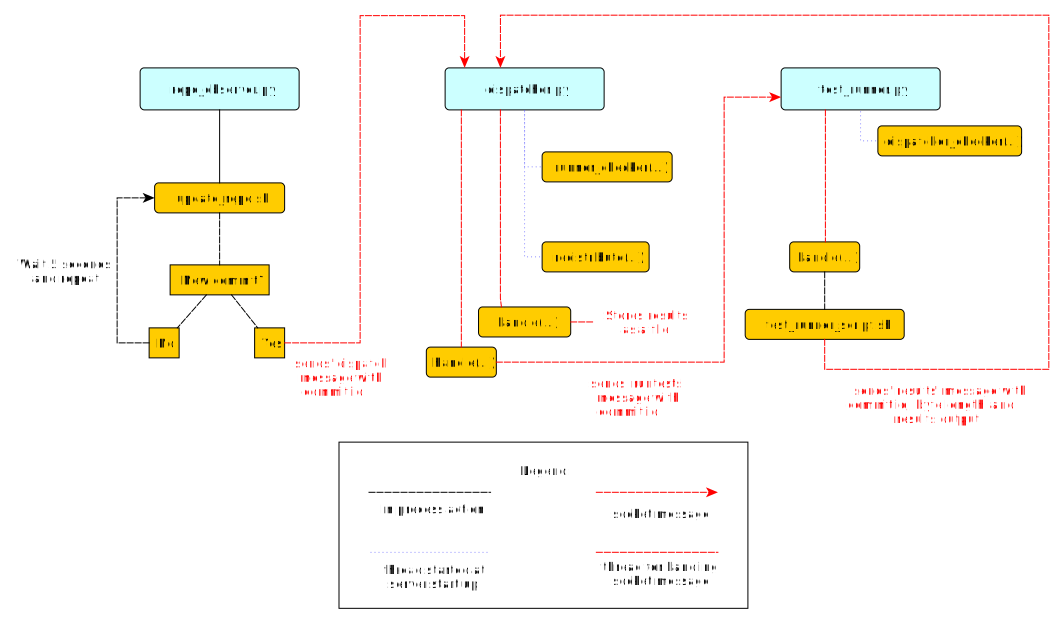
\includegraphics{diagram.svg}

\aosasectii{Running the Code}\label{running-the-code}

We can run this simple CI system locally, using three different terminal
shells for each process.

We start the dispatcher first, running on port 8888:

\begin{aosadescription}

\item[``]
\$ python dispatcher.py
\end{aosadescription}

\begin{center}\rule{3in}{0.4pt}\end{center}

In a new shell, we start the test runner (so it can register itself with
the dispatcher):

\begin{aosadescription}

\item[``]
\$ python test\_runner.py
\textless{}path/to/test\_repo\_clone\_runner\textgreater{}
\end{aosadescription}

\begin{center}\rule{3in}{0.4pt}\end{center}

The test runner will assign itself its own port, in the range 8900-9000.
You may run as many test runners as you like.

Lastly, in another new shell, let's start the repo observer:

\begin{aosadescription}

\item[``]
\$ python repo\_observer.py --dispatcher-server=localhost:8888
\textless{}path/to/test\_repo\_clone\_obs\textgreater{}
\end{aosadescription}

\begin{center}\rule{3in}{0.4pt}\end{center}

Now that everything is set up, let's trigger some tests! To do that,
we'll need to make a new commit. Go to your master repository and make
an arbitrary change:

\begin{aosadescription}

\item[``]
\$ cd /path/to/test\_repo \$ touch new\_file \$ git add new\_file \$ git
commit -m``new file'' new\_file
\end{aosadescription}

\begin{center}\rule{3in}{0.4pt}\end{center}

Then repo\_observer.py will realize that there's a new commit and notify
the dispatcher. You can see the output in their respective shells, so
you can monitor them. Once the dispatcher receives the test results, it
stores them in a test\_results/ folder in this code base, using the
commit ID as the filename.

\aosasecti{Error Handling}\label{error-handling}

This CI system includes some simple error handling.

If you kill the test\_runner.py process, dispatcher.py will figure out
that the runner is no longer available and will remove it from the pool.

You can also kill the test runner, to simulate a machine crash or
network failure. If you do so, the dispatcher will realize the runner
went down and will give another test runner the job if one is available
in the pool, or will wait for a new test runner to register itself in
the pool.

If you kill the dispatcher, the repository observer will figure out it
went down and will throw an exception. The test runners will also
notice, and shut down.

\aosasecti{Conclusion}\label{conclusion}

By separating concerns into their own processes, we were able to build
the fundamentals of a distributed continuous integration system. With
processes communicating with each other via socket requests, we are able
to distribute the system across multiple machines, helping to make our
system more reliable and scalable.

Since the CI system is quite simple now, you can extend it yourself to
be far more functional. Here are a few suggestions for improvements:

\aosasectii{Per-Commit Test Runs}\label{per-commit-test-runs}

The current system will periodically check to see if new commits are run
and will run the most recent commit. This should be improved to test
each commit. To do this, you can modify the periodic checker to dispatch
test runs for each commit in the log between the last tested commit and
the latest commit.

\aosasectii{Smarter Test Runners}\label{smarter-test-runners}

If the test runner detects that the dispatcher is unresponsive, it stops
running. This happens even when the test runner is in the middle of
running tests! It would be better if the test runner waited for a period
of time (or indefinitely, if you do not care about resource management)
for the dispatcher to come back online. In this case, if the dispatcher
goes down while the test runner is actively running a test, instead of
shutting down it will complete the test and wait for the dispatcher to
come back online, and will report the results to it. This will ensure
that we don't waste any effort the test runner makes, and that we will
only run tests once per commit.

\aosasectii{Real Reporting}\label{real-reporting}

In a real CI system, you would have the test results report to a
reporter service which would gather the results, post them somewhere for
people to review, and notify a list of interested parties when a failure
or other notable event occurs. You can extend our simple CI system by
creating a new process to get the reported results, instead of the
dispatcher gathering the results. This new process could be a web server
(or can connect to a web server) which could post the results online,
and may use a mail server to alert subscribers to any test failures.

\aosasectii{Test Runner Manager}\label{test-runner-manager}

Right now, you have to manually launch the test\_runner.py file to start
a test runner. Instead, you could create a test runner manager process
which would assess the current load of test requests from the dispatcher
and scale the number of active test runners accordingly. This process
will receive the runtest messages and will start a test runner process
for each request, and will kill unused processes when the load
decreases.

Using these suggestions, you can make this simple CI system more robust
and fault-tolerant, and you can integrate it with other systems, like a
web-based test reporter.

If you wish to see the level of flexibility continuous integration
systems can achieve, I recommend looking into
\href{http://jenkins-ci.org/}{Jenkins}, a very robust, open-source CI
system written in Java. It provides you with a basic CI system which you
can extend using plugins. You may also access its source code
\href{https://github.com/jenkinsci/jenkins/}{through GitHub}. Another
recommended project is \href{https://travis-ci.org/}{Travis CI}, which
is written in Ruby and whose source code is also available
\href{https://github.com/travis-ci/travis-ci}{through GitHub}.

This has been an exercise in understanding how CI systems work, and how
to build one yourself. You should now have a more solid understanding of
what is needed to make a reliable distributed system, and you can now
use this knowledge to develop more complex solutions.

\end{aosachapter}


\begin{aosachapter}{A Web Crawler With asyncio Coroutines}{s:crawler}{A. Jesse Jiryu Davis and Guido van Rossum}

\emph{A. Jesse Jiryu Davis is a staff engineer at MongoDB in New York.
He wrote Motor, the async MongoDB Python driver, and he is the lead
developer of the MongoDB C Driver and a member of the PyMongo team. He
contributes to asyncio and Tornado. He writes at
\url{http://emptysqua.re}.}

\emph{Guido van Rossum is the creator of Python, one of the major
programming languages on and off the web. The Python community refers to
him as the BDFL (Benevolent Dictator For Life), a title straight from a
Monty Python skit. Guido's home on the web is
\url{http://www.python.org/~guido/}.}

\aosasecti{Introduction}\label{introduction}

Classical computer science emphasizes efficient algorithms that complete
computations as quickly as possible. But many networked programs spend
their time not computing, but holding open many connections that are
slow, or have infrequent events. These programs present a very different
challenge: to wait for a huge number of network events efficiently. A
contemporary approach to this problem is asynchronous I/O, or ``async''.

This chapter presents a simple web crawler. The crawler is an archetypal
async application because it waits for many responses, but does little
computation. The more pages it can fetch at once, the sooner it
completes. If it devotes a thread to each in-flight request, then as the
number of concurrent requests rises it will run out of memory or other
thread-related resource before it runs out of sockets. It avoids the
need for threads by using asynchronous I/O.

We present the example in three stages. First, we show an async event
loop and sketch a crawler that uses the event loop with callbacks: it is
very efficient, but extending it to more complex problems would lead to
unmanageable spaghetti code. Second, therefore, we show that Python
coroutines are both efficient and extensible. We implement simple
coroutines in Python using generator functions. In the third stage, we
use the full-featured coroutines from Python's standard ``asyncio''
library\footnote{Guido introduced the standard asyncio library, called
  ``Tulip'' then, at PyCon 2013.}, and coordinate them using an async
queue.

\aosasecti{The Task}\label{the-task}

A web crawler finds and downloads all pages on a website, perhaps to
archive or index them. Beginning with a root URL, it fetches each page,
parses it for links to pages it has not seen, and adds the new links to
a queue. When it fetches a page with no unseen links and the queue is
empty, it stops.

We can hasten this process by downloading many pages concurrently. As
the crawler finds new links, it launches simultaneous fetch operations
for the new pages on separate sockets. It parses responses as they
arrive, adding new links to the queue. There may come some point of
diminishing returns where too much concurrency degrades performance, so
we cap the number of concurrent requests, and leave the remaining links
in the queue until some in-flight requests complete.

\aosasecti{The Traditional Approach}\label{the-traditional-approach}

How do we make the crawler concurrent? Traditionally we would create a
thread pool. Each thread would be in charge of downloading one page at a
time over a socket. For example, to download a page from xkcd.com:

\begin{verbatim}
def fetch(url):
    sock = socket.socket()
    sock.connect(('xkcd.com', 80))
    request = 'GET {} HTTP/1.0\r\nHost: xkcd.com\r\n\r\n'.format(url)
    sock.send(request.encode('ascii'))
    response = b''
    chunk = sock.recv(4096)
    while chunk:
        response += chunk
        chunk = sock.recv(4096)
    
    # Page is now downloaded.
    links = parse_links(response)
    q.add(links)
\end{verbatim}

By default, socket operations are \emph{blocking}: when the thread calls
a method like \texttt{connect} or \texttt{recv}, it pauses until the
operation completes.\footnote{Even calls to \texttt{send} can block, if
  the recipient is slow to acknowledge outstanding messages and the
  system's buffer of outgoing data is full.} Consequently to download
many pages at once, we need many threads. A sophisticated application
amortizes the cost of thread-creation by keeping idle threads in a
thread pool, then checking them out to reuse them for subsequent tasks;
it does the same with sockets in a connection pool.

And yet, threads are expensive, and operating systems enforce a variety
of hard caps on the number of threads a process, user, or machine may
have. On Jesse's system, a Python thread costs around 50k of memory, and
starting tens of thousands of threads causes failures. If we scale up to
tens of thousands of simultaneous operations on concurrent sockets, we
run out of threads before we run out of sockets. Per-thread overhead or
system limits on threads are the bottleneck.

In his influential article ``The C10K problem''\footnote{\url{http://www.kegel.com/c10k.html}},
Dan Kegel outlines the limitations of multithreading for I/O
concurrency. He begins,

\begin{quote}
It's time for web servers to handle ten thousand clients simultaneously,
don't you think? After all, the web is a big place now.
\end{quote}

Kegel coined the term ``C10K'' in 1999. Ten thousand connections sounds
dainty now, but the problem has changed only in size, not in kind. Back
then, using a thread per connection for C10K was impractical. Now the
cap is orders of magnitude higher. Indeed, our toy web crawler would
work just fine with threads. Yet for very large scale applications, with
hundreds of thousands of connections, the cap remains: there is a limit
beyond which most systems can still create sockets, but have run out of
threads. How can we overcome this?

\aosasecti{Async}\label{async}

Asynchronous I/O frameworks do concurrent operations on a single thread.
Let us find out how.

Async frameworks use \emph{non-blocking} sockets. In our async crawler,
we set the socket non-blocking before we begin to connect to the server:

\begin{verbatim}
sock = socket.socket()
sock.setblocking(False)
try:
    sock.connect(('xkcd.com', 80))
except BlockingIOError:
    pass
\end{verbatim}

Irritatingly, a non-blocking socket throws an exception from
\texttt{connect}, even when it is working normally. This exception
replicates the irritating behavior of the underlying C function, which
sets \texttt{errno} to \texttt{EINPROGRESS} to tell you it has begun.

Now our crawler needs a way to know when the connection is established,
so it can send the HTTP request. We could simply keep trying in a tight
loop:

\begin{verbatim}
request = 'GET {} HTTP/1.0\r\nHost: xkcd.com\r\n\r\n'.format(url)
encoded = request.encode('ascii')

while True:
    try:
        sock.send(encoded)
        break  # Done.
    except OSError as e:
        pass

print('sent')
\end{verbatim}

This method not only wastes electricity, but it cannot efficiently await
events on \emph{multiple} sockets. In ancient times, BSD Unix's solution
to this problem was \texttt{select}, a C function that waits for an
event to occur on a non-blocking socket or a small array of them.
Nowadays the demand for Internet applications with huge numbers of
connections has led to replacements like \texttt{poll}, then
\texttt{kqueue} on BSD and \texttt{epoll} on Linux. These APIs are
similar to \texttt{select}, but perform well with very large numbers of
connections.

Python 3.4's \texttt{DefaultSelector} uses the best \texttt{select}-like
function available on your system. To register for notifications about
network I/O, we create a non-blocking socket and register it with the
default selector:

\begin{verbatim}
from selectors import DefaultSelector, EVENT_WRITE

selector = DefaultSelector()

sock = socket.socket()
sock.setblocking(False)
try:
    sock.connect(('xkcd.com', 80))
except BlockingIOError:
    pass

def connected():
    selector.unregister(sock.fileno())
    print('connected!')

selector.register(sock.fileno(), EVENT_WRITE, connected)
\end{verbatim}

We disregard the spurious error and call \texttt{selector.register},
passing in the socket's file descriptor and a constant that expresses
what event we are waiting for. To be notified when the connection is
established, we pass \texttt{EVENT\_WRITE}: that is, we want to know
when the socket is ``writable''. We also pass a Python function,
\texttt{connected}, to run when that event occurs. Such a function is
known as a \emph{callback}.

We process I/O notifications as the selector receives them, in a loop:

\begin{verbatim}
def loop():
    while True:
        events = selector.select()
        for event_key, event_mask in events:
            callback = event_key.data
            callback()
\end{verbatim}

The \texttt{connected} callback is stored as \texttt{event\_key.data},
which we retrieve and execute once the non-blocking socket is connected.

Unlike in our fast-spinning loop above, the call to \texttt{select} here
pauses, awaiting the next I/O events. Then the loop runs callbacks that
are waiting for these events. Operations that have not completed remain
pending until some future tick of the event loop.

What have we demonstrated already? We showed how to begin an operation
and execute a callback when the operation is ready. An async
\emph{framework} builds on the two features we have shown---non-blocking
sockets and the event loop---to run concurrent operations on a single
thread.

We have achieved ``concurrency'' here, but not what is traditionally
called ``parallelism''. That is, we built a tiny system that does
overlapping I/O. It is capable of beginning new operations while others
are in flight. It does not actually utilize multiple cores to execute
computation in parallel. But then, this system is designed for I/O-bound
problems, not CPU-bound ones.\footnote{Python's global interpreter lock
  prohibits running Python code in parallel in one process anyway.
  Parallelizing CPU-bound algorithms in Python requires multiple
  processes, or writing the parallel portions of the code in C. But that
  is a topic for another day.}

So our event loop is efficient at concurrent I/O because it does not
devote thread resources to each connection. But before we proceed, it is
important to correct a common misapprehension that async is
\emph{faster} than multithreading. Often it is not---indeed, in Python,
an event loop like ours is moderately slower than multithreading at
serving a small number of very active connections. In a runtime without
a global interpreter lock, threads would perform even better on such a
workload. What asynchronous I/O is right for, is applications with many
slow or sleepy connections with infrequent events.\footnote{Jesse listed
  indications and contraindications for using async in ``What Is Async,
  How Does It Work, And When Should I Use It?'', available at
  pyvideo.org.}\footnote{Mike Bayer compared the throughput of asyncio
  and multithreading for different workloads in his ``Asynchronous
  Python and Databases'':
  http://techspot.zzzeek.org/2015/02/15/asynchronous-python-and-databases/}

\aosasecti{Programming With Callbacks}\label{programming-with-callbacks}

With the runty async framework we have built so far, how can we build a
web crawler? Even a simple URL-fetcher is painful to write.

We begin with global sets of the URLs we have yet to fetch, and the URLs
we have seen:

\begin{verbatim}
urls_todo = set(['/'])
seen_urls = set(['/'])
\end{verbatim}

The \texttt{seen\_urls} set includes \texttt{urls\_todo} plus completed
URLs. The two sets are initialized with the root URL ``/''.

Fetching a page will require a series of callbacks. The
\texttt{connected} callback fires when a socket is connected, and sends
a GET request to the server. But then it must await a response, so it
registers another callback. If, when that callback fires, it cannot read
the full response yet, it registers again, and so on.

Let us collect these callbacks into a \texttt{Fetcher} object. It needs
a URL, a socket object, and a place to accumulate the response bytes:

\begin{verbatim}
class Fetcher:
    def __init__(self, url):
        self.response = b''  # Empty array of bytes.
        self.url = url
        self.sock = None
\end{verbatim}

We begin by calling \texttt{Fetcher.fetch}:

\begin{verbatim}
    # Method on Fetcher class.
    def fetch(self):
        self.sock = socket.socket()
        self.sock.setblocking(False)
        try:
            self.sock.connect(('xkcd.com', 80))
        except BlockingIOError:
            pass
            
        # Register next callback.
        selector.register(self.sock.fileno(),
                          EVENT_WRITE,
                          self.connected)
\end{verbatim}

The \texttt{fetch} method begins connecting a socket. But notice the
method returns before the connection is established. It must return
control to the event loop to wait for the connection. To understand why,
imagine our whole application was structured so:

\begin{verbatim}
# Begin fetching http://xkcd.com/353/
fetcher = Fetcher('/353/')
fetcher.fetch()

while True:
    events = selector.select()
    for event_key, event_mask in events:
        callback = event_key.data
        callback(event_key, event_mask)
\end{verbatim}

All event notifications are processed in the event loop when it calls
\texttt{select}. Hence \texttt{fetch} must hand control to the event
loop, so that the program knows when the socket has connected. Only then
does the loop run the \texttt{connected} callback, which was registered
at the end of \texttt{fetch} above.

Here is the implementation of \texttt{connected}:

\begin{verbatim}
    # Method on Fetcher class.
    def connected(self, key, mask):
        print('connected!')
        selector.unregister(key.fd)
        request = 'GET {} HTTP/1.0\r\nHost: xkcd.com\r\n\r\n'.format(self.url)
        self.sock.send(request.encode('ascii'))
        
        # Register the next callback.
        selector.register(key.fd,
                          EVENT_READ,
                          self.read_response)
\end{verbatim}

The method sends a GET request. A real application would check the
return value of \texttt{send} in case the whole message cannot be sent
at once. But our request is small and our application unsophisticated.
It blithely calls \texttt{send}, then waits for a response. Of course,
it must register yet another callback and relinquish control to the
event loop. The next and final callback, \texttt{read\_response},
processes the server's reply:

\begin{verbatim}
    # Method on Fetcher class.
    def read_response(self, key, mask):
        global stopped

        chunk = self.sock.recv(4096)  # 4k chunk size.
        if chunk:
            self.response += chunk
        else:
            selector.unregister(key.fd)  # Done reading.
            links = self.parse_links()
            
            # Python set-logic:
            for link in links.difference(seen_urls):
                urls_todo.add(link)
                Fetcher(link).fetch()  # <- New Fetcher.

            seen_urls.update(links)
            urls_todo.remove(self.url)
            if not urls_todo:
                stopped = True
\end{verbatim}

The callback is executed each time the selector sees that the socket is
``readable'', which could mean two things: the socket has data or it is
closed.

The callback asks for up to four kilobytes of data from the socket. If
less is ready, \texttt{chunk} contains whatever data is available. If
there is more, \texttt{chunk} is four kilobytes long and the socket
remains readable, so the event loop runs this callback again on the next
tick. When the response is complete, the server has closed the socket
and \texttt{chunk} is empty.

The \texttt{parse\_links} method, not shown, returns a set of URLs. We
start a new fetcher for each new URL, with no concurrency cap. Note a
nice feature of async programming with callbacks: we need no mutex
around changes to shared data, such as when we add links to
\texttt{seen\_urls}. There is no preemptive multitasking, so we cannot
be interrupted at arbitrary points in our code.

We add a global \texttt{stopped} variable and use it to control the
loop:

\begin{verbatim}
stopped = False

def loop():
    while not stopped:
        events = selector.select()
        for event_key, event_mask in events:
            callback = event_key.data
            callback()
\end{verbatim}

Once all pages are downloaded the fetcher stops the global event loop
and the program exits.

This example makes async's problem plain: spaghetti code.

We need some way to express a series of computations and I/O operations,
and schedule multiple such series of operations to run concurrently. But
without threads, a series of operations cannot be collected into a
single function: whenever a function begins an I/O operation, it
explicitly saves whatever state will be needed in the future, then
returns. You are responsible for thinking about and writing this
state-saving code.

Let us explain what we mean by that. Consider how simply we fetched a
URL on a thread with a conventional blocking socket:

\begin{verbatim}
# Blocking version.
def fetch(url):
    sock = socket.socket()
    sock.connect(('xkcd.com', 80))
    request = 'GET {} HTTP/1.0\r\nHost: xkcd.com\r\n\r\n'.format(url)
    sock.send(request.encode('ascii'))
    response = b''
    chunk = sock.recv(4096)
    while chunk:
        response += chunk
        chunk = sock.recv(4096)
    
    # Page is now downloaded.
    links = parse_links(response)
    q.add(links)
\end{verbatim}

What state does this function remember between one socket operation and
the next? It has the socket, a URL, and the accumulating
\texttt{response}. A function that runs on a thread uses basic features
of the programming language to store this temporary state in local
variables, on its stack. The function also has a ``continuation''---that
is, the code it plans to execute after I/O completes. The runtime
remembers the continuation by storing the thread's instruction pointer.
You need not think about restoring these local variables and the
continuation after I/O. It is built in to the language.

But with a callback-based async framework, these language features are
no help. While waiting for I/O, a function must save its state
explicitly, because the function returns and loses its stack frame
before I/O completes. In lieu of local variables, our callback-based
example stores \texttt{sock} and \texttt{response} as attributes of
\texttt{self}, the Fetcher instance. In lieu of the instruction pointer,
it stores its continuation by registering the callbacks
\texttt{connected} and \texttt{read\_response}. As the application's
features grow, so does the complexity of the state we manually save
across callbacks. Such onerous bookkeeping makes the coder prone to
migraines.

Even worse, what happens if a callback throws an exception, before it
schedules the next callback in the chain? Say we did a poor job on the
\texttt{parse\_links} method and it throws an exception parsing some
HTML:

\begin{verbatim}
Traceback (most recent call last):
  File "loop-with-callbacks.py", line 111, in <module>
    loop()
  File "loop-with-callbacks.py", line 106, in loop
    callback(event_key, event_mask)
  File "loop-with-callbacks.py", line 51, in read_response
    links = self.parse_links()
  File "loop-with-callbacks.py", line 67, in parse_links
    raise Exception('parse error')
Exception: parse error
\end{verbatim}

The stack trace shows only that the event loop was running a callback.
We do not remember what led to the error. The chain is broken on both
ends: we forgot where we were going and whence we came. This loss of
context is called ``stack ripping'', and in many cases it confounds the
investigator. Stack ripping also prevents us from installing an
exception handler for a chain of callbacks, the way a ``try / except''
block wraps a function call and its tree of descendents.\footnote{For a
  complex solution to this problem, see
  \url{http://www.tornadoweb.org/en/stable/stack_context.html}}

So, even apart from the long debate about the relative efficiencies of
multithreading and async, there is this other debate regarding which is
more error-prone: threads are susceptible to data races if you make a
mistake synchronizing them, but callbacks are stubborn to debug due to
stack ripping.

\aosasecti{Coroutines}\label{coroutines}

We entice you with a promise. It is possible to write asynchronous code
that combines the efficiency of callbacks with the classic good looks of
multithreaded programming. This combination is achieved with a pattern
called ``coroutines''. Using Python 3.4's standard asyncio library, and
a package called ``aiohttp'', fetching a URL in a coroutine is very
direct\footnote{The \texttt{@asyncio.coroutine} decorator is not
  magical. In fact, if it decorates a generator function and the
  \texttt{PYTHONASYNCIODEBUG} environment variable is not set, the
  decorator does practically nothing. It just sets an attribute,
  \texttt{\_is\_coroutine}, for the convenience of other parts of the
  framework. It is possible to use asyncio with bare generators not
  decorated with \texttt{@asyncio.coroutine} at all.}:

\begin{verbatim}
    @asyncio.coroutine
    def fetch(self, url):
        response = yield from self.session.get(url)
        body = yield from response.read()
\end{verbatim}

It is also scalable. Compared to the 50k of memory per thread and the
operating system's hard limits on threads, a Python coroutine takes
barely 3k of memory on Jesse's system. Python can easily start hundreds
of thousands of coroutines.

The concept of a coroutine, dating to the elder days of computer
science, is simple: it is a subroutine that can be paused and resumed.
Whereas threads are preemptively multitasked by the operating system,
coroutines multitask cooperatively: they choose when to pause, and which
coroutine to run next.

There are many implementations of coroutines; even in Python there are
several. The coroutines in the standard ``asyncio'' library in Python
3.4 are built upon generators, a Future class, and the ``yield from''
statement. Starting in Python 3.5, coroutines are a native feature of
the language itself\footnote{Python 3.5's built-in coroutines are
  described in \href{https://www.python.org/dev/peps/pep-0492/}{PEP
  492}, ``Coroutines with async and await syntax.''}; however,
understanding coroutines as they were first implemented in Python 3.4,
using pre-existing language facilities, is the foundation to tackle
Python 3.5's native coroutines.

To explain Python 3.4's generator-based coroutines, we will engage in an
exposition of generators and how they are used as coroutines in asyncio,
and trust you will enjoy reading it as much as we enjoyed writing it.
Once we have explained generator-based coroutines, we shall use them in
our async web crawler.

\aosasecti{How Python Generators Work}\label{how-python-generators-work}

Before you grasp Python generators, you have to understand how regular
Python functions work. Normally, when a Python function calls a
subroutine, the subroutine retains control until it returns, or throws
an exception. Then control returns to the caller:

\begin{verbatim}
>>> def foo():
...     bar()
...
>>> def bar():
...     pass
\end{verbatim}

The standard Python interpreter is written in C. The C function that
executes a Python function is called, mellifluously,
\texttt{PyEval\_EvalFrameEx}. It takes a Python stack frame object and
evaluates Python bytecode in the context of the frame. Here is the
bytecode for \texttt{foo}:

\begin{verbatim}
>>> import dis
>>> dis.dis(foo)
  2           0 LOAD_GLOBAL              0 (bar)
              3 CALL_FUNCTION            0 (0 positional, 0 keyword pair)
              6 POP_TOP
              7 LOAD_CONST               0 (None)
             10 RETURN_VALUE
\end{verbatim}

The \texttt{foo} function loads \texttt{bar} onto its stack and calls
it, then pops its return value from the stack, loads \texttt{None} onto
the stack, and returns \texttt{None}.

When \texttt{PyEval\_EvalFrameEx} encounters the \texttt{CALL\_FUNCTION}
bytecode, it creates a new Python stack frame and recurses: that is, it
calls \texttt{PyEval\_EvalFrameEx} recursively with the new frame, which
is used to execute \texttt{bar}.

\aosafigure[240pt]{crawler-images/function-calls.png}{Function Calls}{500l.crawler.functioncalls}

It is crucial to understand that Python stack frames are allocated in
heap memory! The Python interpreter is a normal C program, so its stack
frames are normal stack frames. But the \emph{Python} stack frames it
manipulates are on the heap. Among other surprises, this means a Python
stack frame can outlive its function call. To see this interactively,
save the current frame from within \texttt{bar}:

\begin{verbatim}
>>> import inspect
>>> frame = None
>>> def foo():
...     bar()
...
>>> def bar():
...     global frame
...     frame = inspect.currentframe()
...
>>> foo()
>>> # The frame was executing the code for 'bar'.
>>> frame.f_code.co_name
'bar'
>>> # Its back pointer refers to the frame for 'foo'.
>>> caller_frame = frame.f_back
>>> caller_frame.f_code.co_name
'foo'
\end{verbatim}

The stage is now set for Python generators, which use the same building
blocks---code objects and stack frames---to marvelous effect.

This is a generator function:

\begin{verbatim}
>>> def gen_fn():
...     result = yield 1
...     print('result of yield: {}'.format(result))
...     result2 = yield 2
...     print('result of 2nd yield: {}'.format(result2))
...     return 'done'
...     
\end{verbatim}

When Python compiles \texttt{gen\_fn} to bytecode, it sees the
\texttt{yield} statement and knows that \texttt{gen\_fn} is a generator
function, not a regular one. It sets a flag to remember this fact:

\begin{verbatim}
>>> # The generator flag is bit position 5.
>>> generator_bit = 1 << 5
>>> bool(gen_fn.__code__.co_flags & generator_bit)
True
\end{verbatim}

When you call a generator function, Python sees the generator flag, and
it does not actually run the function. Instead, it creates a generator:

\begin{verbatim}
>>> gen = gen_fn()
>>> type(gen)
<class 'generator'>
\end{verbatim}

A Python generator encapsulates a stack frame plus a reference to some
code, the body of \texttt{gen\_fn}:

\begin{verbatim}
>>> gen.gi_code.co_name
'gen_fn'
\end{verbatim}

All generators from calls to \texttt{gen\_fn} point to this same code.
But each has its own stack frame. This stack frame is not on any actual
stack, it sits in heap memory waiting to be used:

\aosafigure[240pt]{crawler-images/generator.png}{Generators}{500l.crawler.generators}

The frame has a ``last instruction'' pointer, the instruction it
executed most recently. In the beginning, the last instruction pointer
is -1, meaning the generator has not begun:

\begin{verbatim}
>>> gen.gi_frame.f_lasti
-1
\end{verbatim}

When we call \texttt{send}, the generator reaches its first
\texttt{yield}, and pauses. The return value of \texttt{send} is 1,
since that is what \texttt{gen} passes to the \texttt{yield} expression:

\begin{verbatim}
>>> gen.send(None)
1
\end{verbatim}

The generator's instruction pointer is now 3 bytecodes from the start,
part way through the 56 bytes of compiled Python:

\begin{verbatim}
>>> gen.gi_frame.f_lasti
3
>>> len(gen.gi_code.co_code)
56
\end{verbatim}

The generator can be resumed at any time, from any function, because its
stack frame is not actually on the stack: it is on the heap. Its
position in the call hierarchy is not fixed, and it need not obey the
first-in, last-out order of execution that regular functions do. It is
liberated, floating free like a cloud.

We can send the value ``hello'' into the generator and it becomes the
result of the \texttt{yield} expression, and the generator continues
until it yields 2:

\begin{verbatim}
>>> gen.send('hello')
result of yield: hello
2
\end{verbatim}

Its stack frame now contains the local variable \texttt{result}:

\begin{verbatim}
>>> gen.gi_frame.f_locals
{'result': 'hello'}
\end{verbatim}

Other generators created from \texttt{gen\_fn} will have their own stack
frames and their own local variables.

When we call \texttt{send} again, the generator continues from its
second \texttt{yield}, and finishes by raising the special
\texttt{StopIteration} exception:

\begin{verbatim}
>>> gen.send('goodbye')
result of 2nd yield: goodbye
Traceback (most recent call last):
  File "<input>", line 1, in <module>
StopIteration: done
\end{verbatim}

The exception has a value, which is the return value of the generator:
the string ``done''.

\aosasecti{Building Coroutines With
Generators}\label{building-coroutines-with-generators}

So a generator can pause, and it can be resumed with a value, and it has
a return value. Sounds like a good primitive upon which to build an
async programming model, without spaghetti callbacks! We want to build a
``coroutine'': a routine that is cooperatively scheduled with other
routines in the program. Our coroutines will be a simplified version of
those in Python's standard ``asyncio'' library. As in asyncio, we will
use generators, futures, and the ``yield from'' statement.

First we need a way to represent some future result that a coroutine is
waiting for. A stripped-down version:

\begin{verbatim}
class Future:
    def __init__(self):
        self.result = None
        self._callbacks = []

    def add_done_callback(self, fn):
        self._callbacks.append(fn)

    def set_result(self, result):
        self.result = result
        for fn in self._callbacks:
            fn(self)
\end{verbatim}

A future is initially ``pending''. It is ``resolved'' by a call to
\texttt{set\_result}.\footnote{This future has many deficiencies. For
  example, once this future is resolved, a coroutine that yields it
  should resume immediately instead of pausing, but with our code it
  does not. See asyncio's Future class for a complete implementation.}

Let us adapt our fetcher to use futures and coroutines. Review how we
wrote \texttt{fetch} with a callback:

\begin{verbatim}
class Fetcher:
    def fetch(self):
        self.sock = socket.socket()
        self.sock.setblocking(False)
        try:
            self.sock.connect(('xkcd.com', 80))
        except BlockingIOError:
            pass
        selector.register(self.sock.fileno(),
                          EVENT_WRITE,
                          self.connected)

    def connected(self, key, mask):
        print('connected!')
        # And so on....
\end{verbatim}

The \texttt{fetch} method begins connecting a socket, then registers the
callback, \texttt{connected}, to be executed when the socket is ready.
Now we can combine these two steps into one coroutine:

\begin{verbatim}
    def fetch(self):
        sock = socket.socket()
        sock.setblocking(False)
        try:
            sock.connect(('xkcd.com', 80))
        except BlockingIOError:
            pass

        f = Future()

        def on_connected():
            f.set_result(None)

        selector.register(sock.fileno(),
                          EVENT_WRITE,
                          on_connected)
        yield f
        selector.unregister(sock.fileno())
        print('connected!')
\end{verbatim}

Now \texttt{fetch} is a generator function, rather than a regular one,
because it contains a \texttt{yield} statement. We create a pending
future, then yield it to pause \texttt{fetch} until the socket is ready.
The inner function \texttt{on\_connected} resolves the future.

But when the future resolves, what resumes the generator? We need a
coroutine \emph{driver}. Let us call it ``task'':

\begin{verbatim}
class Task:
    def __init__(self, coro):
        self.coro = coro
        f = Future()
        f.set_result(None)
        self.step(f)

    def step(self, future):
        try:
            next_future = self.coro.send(future.result)
        except StopIteration:
            return

        next_future.add_done_callback(self.step)

# Begin fetching http://xkcd.com/353/
fetcher = Fetcher('/353/')
Task(fetcher.fetch())

loop()
\end{verbatim}

The task starts the \texttt{fetch} generator by sending \texttt{None}
into it. Then \texttt{fetch} runs until it yields a future, which the
task captures as \texttt{next\_future}. When the socket is connected,
the event loop runs the callback \texttt{on\_connected}, which resolves
the future, which calls \texttt{step}, which resumes \texttt{fetch}.

\aosasecti{Factoring Coroutines With
\texttt{yield from}}\label{factoring-coroutines-with-yield-from}

Once the socket is connected, we send the HTTP GET request and read the
server response. These steps need no longer be scattered among
callbacks; we gather them into the same generator function:

\begin{verbatim}
    def fetch(self):
        # ... connection logic from above, then:
        sock.send(request.encode('ascii'))

        while True:
            f = Future()

            def on_readable():
                f.set_result(sock.recv(4096))

            selector.register(sock.fileno(),
                              EVENT_READ,
                              on_readable)
            chunk = yield f
            selector.unregister(sock.fileno())
            if chunk:
                self.response += chunk
            else:
                # Done reading.
                break
\end{verbatim}

This code, which reads a whole message from a socket, seems generally
useful. How can we factor it from \texttt{fetch} into a subroutine? Now
Python 3's celebrated \texttt{yield from} takes the stage. It lets one
generator \emph{delegate} to another.

To see how, let us return to our simple generator example:

\begin{verbatim}
>>> def gen_fn():
...     result = yield 1
...     print('result of yield: {}'.format(result))
...     result2 = yield 2
...     print('result of 2nd yield: {}'.format(result2))
...     return 'done'
...     
\end{verbatim}

To call this generator from another generator, delegate to it with
\texttt{yield from}:

\begin{verbatim}
>>> # Generator function:
>>> def caller_fn():
...     gen = gen_fn()
...     rv = yield from gen
...     print('return value of yield-from: {}'
...           .format(rv))
...
>>> # Make a generator from the
>>> # generator function.
>>> caller = caller_fn()
\end{verbatim}

The \texttt{caller} generator acts as if it were \texttt{gen}, the
generator it is delegating to:

\begin{verbatim}
>>> caller.send(None)
1
>>> caller.gi_frame.f_lasti
15
>>> caller.send('hello')
result of yield: hello
2
>>> caller.gi_frame.f_lasti  # Hasn't advanced.
15
>>> caller.send('goodbye')
result of 2nd yield: goodbye
return value of yield-from: done
Traceback (most recent call last):
  File "<input>", line 1, in <module>
StopIteration
\end{verbatim}

While \texttt{caller} yields from \texttt{gen}, \texttt{caller} does not
advance. Notice that its instruction pointer remains at 15, the site of
its \texttt{yield from} statement, even while the inner generator
\texttt{gen} advances from one \texttt{yield} statement to the
next.\footnote{In fact, this is exactly how ``yield from'' works in
  CPython. A function increments its instruction pointer before
  executing each statement. But after the outer generator executes
  ``yield from'', it subtracts 1 from its instruction pointer to keep
  itself pinned at the ``yield from'' statement. Then it yields to
  \emph{its} caller. The cycle repeats until the inner generator throws
  \texttt{StopIteration}, at which point the outer generator finally
  allows itself to advance to the next instruction.} From our
perspective outside \texttt{caller}, we cannot tell if the values it
yields are from \texttt{caller} or from the generator it delegates to.
And from inside \texttt{gen}, we cannot tell if values are sent in from
\texttt{caller} or from outside it. The \texttt{yield from} statement is
a frictionless channel, through which values flow in and out of
\texttt{gen} until \texttt{gen} completes.

A coroutine can delegate work to a sub-coroutine with
\texttt{yield from} and receive the result of the work. Notice, above,
that \texttt{caller} printed ``return value of yield-from: done''. When
\texttt{gen} completed, its return value became the value of the
\texttt{yield from} statement in \texttt{caller}:

\begin{verbatim}
    rv = yield from gen
\end{verbatim}

Earlier, when we criticized callback-based async programming, our most
strident complaint was about ``stack ripping'': when a callback throws
an exception, the stack trace is typically useless. It only shows that
the event loop was running the callback, not \emph{why}. How do
coroutines fare?

\begin{verbatim}
>>> def gen_fn():
...     raise Exception('my error')
>>> caller = caller_fn()
>>> caller.send(None)
Traceback (most recent call last):
  File "<input>", line 1, in <module>
  File "<input>", line 3, in caller_fn
  File "<input>", line 2, in gen_fn
Exception: my error
\end{verbatim}

This is much more useful! The stack trace shows \texttt{caller\_fn} was
delegating to \texttt{gen\_fn} when it threw the error. Even more
comforting, we can wrap the call to a sub-coroutine in an exception
handler, the same is with normal subroutines:

\begin{verbatim}
>>> def gen_fn():
...     yield 1
...     raise Exception('uh oh')
...
>>> def caller_fn():
...     try:
...         yield from gen_fn()
...     except Exception as exc:
...         print('caught {}'.format(exc))
...
>>> caller = caller_fn()
>>> caller.send(None)
1
>>> caller.send('hello')
caught uh oh
\end{verbatim}

So we factor logic with sub-coroutines just like with regular
subroutines. Let us factor some useful sub-coroutines from our fetcher.
We write a \texttt{read} coroutine to receive one chunk:

\begin{verbatim}
def read(sock):
    f = Future()

    def on_readable():
        f.set_result(sock.recv(4096))

    selector.register(sock.fileno(), EVENT_READ, on_readable)
    chunk = yield f  # Read one chunk.
    selector.unregister(sock.fileno())
    return chunk
\end{verbatim}

We build on \texttt{read} with a \texttt{read\_all} coroutine that
receives a whole message:

\begin{verbatim}
def read_all(sock):
    response = []
    # Read whole response.
    chunk = yield from read(sock)
    while chunk:
        response.append(chunk)
        chunk = yield from read(sock)

    return b''.join(response)
\end{verbatim}

If you squint the right way, the \texttt{yield from} statements
disappear and these look like conventional functions doing blocking I/O.
But in fact, \texttt{read} and \texttt{read\_all} are coroutines.
Yielding from \texttt{read} pauses \texttt{read\_all} until the I/O
completes. While \texttt{read\_all} is paused, asyncio's event loop does
other work and awaits other I/O events; \texttt{read\_all} is resumed
with the result of \texttt{read} on the next loop tick once its event is
ready.

At the stack's root, \texttt{fetch} calls \texttt{read\_all}:

\begin{verbatim}
class Fetcher:
    def fetch(self):
         # ... connection logic from above, then:
        sock.send(request.encode('ascii'))
        self.response = yield from read_all(sock)
\end{verbatim}

Miraculously, the Task class needs no modification. It drives the outer
\texttt{fetch} coroutine just the same as before:

\begin{verbatim}
Task(fetcher.fetch())
loop()
\end{verbatim}

When \texttt{read} yields a future, the task receives it through the
channel of \texttt{yield from} statements, precisely as if the future
were yielded directly from \texttt{fetch}. When the loop resolves a
future, the task sends its result into \texttt{fetch}, and the value is
received by \texttt{read}, exactly as if the task were driving
\texttt{read} directly:

\aosafigure[240pt]{crawler-images/yield-from.png}{Yield From}{500l.crawler.yieldfrom}

To perfect our coroutine implementation, we polish out one mar: our code
uses \texttt{yield} when it waits for a future, but \texttt{yield from}
when it delegates to a sub-coroutine. It would be more refined if we
used \texttt{yield from} whenever a coroutine pauses. Then a coroutine
need not concern itself with what type of thing it awaits.

We take advantage of the deep correspondence in Python between
generators and iterators. Advancing a generator is, to the caller, the
same as advancing an iterator. So we make our Future class iterable by
implementing a special method:

\begin{verbatim}
    # Method on Future class.
    def __iter__(self):
        # Tell Task to resume me here.
        yield self
        return self.result
\end{verbatim}

The future's \texttt{\_\_iter\_\_} method is a coroutine that yields the
future itself. Now when we replace code like this:

\begin{verbatim}
# f is a Future.
yield f
\end{verbatim}

\ldots{}with this:

\begin{verbatim}
# f is a Future.
yield from f
\end{verbatim}

\ldots{}the outcome is precisely the same! The driving Task receives the
future from its call to \texttt{self.coro.send(result)}, and when the
future is resolved it sends the new result back into the coroutine.

What is the advantage of using \texttt{yield from} everywhere? Why is
that better than waiting for futures with \texttt{yield} and delegating
to sub-coroutines with \texttt{yield from}? It is better because now, a
method can freely change its implementation without affecting the
caller: it might be a normal method that returns a future that will
\emph{resolve} to a value, or it might be a coroutine that contains
\texttt{yield from} statements and \emph{returns} a value. In either
case, the caller need only \texttt{yield from} the method in order to
wait for the result.

Gentle reader, we have reached the end of our enjoyable exposition of
coroutines in asyncio. We peered into the machinery of generators, and
sketched an implementation of futures and tasks. We outlined how asyncio
attains the best of both worlds: concurrent I/O that is more efficient
than threads and more legible than callbacks. Of course, the real
asyncio is much more sophisticated than our sketch. The real framework
addresses zero-copy I/O, fair scheduling, exception handling, and an
abundance of other features.

To an asyncio user, coding with coroutines is much simpler than you saw
here. In the code above we implemented coroutines from first principles,
so you saw callbacks, tasks, and futures. You even saw non-blocking
sockets and the call to \texttt{select}. But when it comes time to build
an application with asyncio, none of this appears in your code. As we
promised, you can fetch a URL as sleekly as this:

\begin{verbatim}
    @asyncio.coroutine
    def fetch(self, url):
        response = yield from self.session.get(url)
        body = yield from response.read()
\end{verbatim}

Satisfied with this exposition, we return to our original assignment: to
write an async web crawler, using asyncio.

\aosasecti{Coordinating Coroutines}\label{coordinating-coroutines}

We began by describing how we want our crawler to work. Now it is time
to implement it with asyncio coroutines.

Our crawler will fetch the first page, parse its links, and add them to
a queue. After this it fans out across the website, fetching pages
concurrently. But to limit load on the client and server, we want some
maximum number of workers to run, and no more. Whenever a worker
finishes fetching a page, it should immediately pull the next link from
the queue. We will pass through periods when there is not enough work to
go around, so some workers must pause. But when a worker hits a page
rich with new links, then the queue suddenly grows and any paused
workers should wake and get cracking. Finally, our program must quit
once its work is done.

Imagine if the workers were threads. How would we express the crawler's
algorithm? We could use a synchronized queue\footnote{\url{https://docs.python.org/3/library/queue.html}}
from the Python standard library. Each time an item is put in the queue,
the queue increments its count of ``tasks''. Worker threads call
\texttt{task\_done} after completing work on an item. The main thread
blocks on \texttt{Queue.join} until each item put in the queue is
matched by a \texttt{task\_done} call, then it exits.

Coroutines use the exact same pattern with a queue from asyncio! First
we import asyncio's queue\footnote{\url{https://docs.python.org/3/library/asyncio-sync.html}}:

\begin{verbatim}
try:
    from asyncio import JoinableQueue as Queue
except ImportError:
    # In Python 3.5, asyncio.JoinableQueue is
    # merged into Queue.
    from asyncio import Queue
\end{verbatim}

We collect the workers' shared state in a crawler class, and write the
main logic in its \texttt{crawl} method. We start \texttt{crawl} on a
coroutine and run asyncio's event loop until \texttt{crawl} finishes:

\begin{verbatim}
loop = asyncio.get_event_loop()

crawler = crawling.Crawler('http://xkcd.com',
                           max_redirect=10)

loop.run_until_complete(crawler.crawl())
\end{verbatim}

The crawler begins with a root URL and \texttt{max\_redirect}, the
number of redirects it is willing to follow to fetch any one URL. It
puts the pair \texttt{(URL, max\_redirect)} in the queue. (For the
reason why, stay tuned.)

\begin{verbatim}
class Crawler:
    def __init__(self, root_url, max_redirect):
        self.max_tasks = 10
        self.max_redirect = max_redirect
        self.q = Queue()
        self.seen_urls = set()
        
        # aiohttp's ClientSession does connection pooling and
        # HTTP keep-alives for us.
        self.session = aiohttp.ClientSession(loop=loop)
        
        # Put (URL, max_redirect) in the queue.
        self.q.put((root_url, self.max_redirect))
\end{verbatim}

The number of unfinished tasks in the queue is now one. Back in our main
script, we launch the event loop and the \texttt{crawl} method:

\begin{verbatim}
loop.run_until_complete(crawler.crawl())
\end{verbatim}

The \texttt{crawl} coroutine kicks off the workers. It is like a main
thread: it blocks on \texttt{join} until all tasks are finished, while
the workers run in the background.

\begin{verbatim}
    @asyncio.coroutine
    def crawl(self):
        """Run the crawler until all work is done."""
        workers = [asyncio.Task(self.work())
                   for _ in range(self.max_tasks)]

        # When all work is done, exit.
        yield from self.q.join()
        for w in workers:
            w.cancel()
\end{verbatim}

If the workers were threads we might not wish to start them all at once.
To avoid creating expensive threads until it is certain they are
necessary, a thread pool typically grows on demand. But coroutines are
cheap, so we simply start the maximum number allowed.

It is interesting to note how we shut down the crawler. When the
\texttt{join} future resolves, the worker tasks are alive but suspended:
they wait for more URLs but none come. So, the main coroutine cancels
them before exiting. Otherwise, as the Python interpreter shuts down and
calls all objects' destructors, living tasks cry out:

\begin{verbatim}
ERROR:asyncio:Task was destroyed but it is pending!
\end{verbatim}

And how does \texttt{cancel} work? Generators have a feature we have not
yet shown you. You can throw an exception into a generator from outside:

\begin{verbatim}
>>> gen = gen_fn()
>>> gen.send(None)  # Start the generator as usual.
1
>>> gen.throw(Exception('error'))
Traceback (most recent call last):
  File "<input>", line 3, in <module>
  File "<input>", line 2, in gen_fn
Exception: error
\end{verbatim}

The generator is resumed by \texttt{throw}, but it is now raising an
exception. If no code in the generator's call stack catches it, the
exception bubbles back up to the top. So to cancel a task's coroutine:

\begin{verbatim}
    # Method of Task class.
    def cancel(self):
        self.coro.throw(CancelledError)
\end{verbatim}

Wherever the generator is paused, at some \texttt{yield from} statement,
it resumes and throws an exception. We handle cancellation in the task's
\texttt{step} method:

\begin{verbatim}
    # Method of Task class.
    def step(self, future):
        try:
            next_future = self.coro.send(future.result)
        except CancelledError:
            self.cancelled = True
            return
        except StopIteration:
            return

        next_future.add_done_callback(self.step)
\end{verbatim}

Now the task knows it is cancelled, so when it is destroyed it does not
rage against the dying of the light.

Once \texttt{crawl} has canceled the workers, it exits. The event loop
sees that the coroutine is complete (we shall see how later), and it too
exits:

\begin{verbatim}
loop.run_until_complete(crawler.crawl())
\end{verbatim}

The \texttt{crawl} method comprises all that our main coroutine must do.
It is the worker coroutines that get URLs from the queue, fetch them,
and parse them for new links. Each worker runs the \texttt{work}
coroutine independently:

\begin{verbatim}
    @asyncio.coroutine
    def work(self):
        while True:
            url, max_redirect = yield from self.q.get()

            # Download page and add new links to self.q.
            yield from self.fetch(url, max_redirect)
            self.q.task_done()
\end{verbatim}

Python sees that this code contains \texttt{yield from} statements, and
compiles it into a generator function. So in \texttt{crawl}, when the
main coroutine calls \texttt{self.work} ten times, it does not actually
execute this method: it only creates ten generator objects with
references to this code. It wraps each in a Task. The Task receives each
future the generator yields, and drives the generator by calling
\texttt{send} with each future's result when the future resolves.
Because the generators have their own stack frames, they run
independently, with separate local variables and instruction pointers.

The worker coordinates with its fellows via the queue. It waits for new
URLs with:

\begin{verbatim}
    url, max_redirect = yield from self.q.get()
\end{verbatim}

The queue's \texttt{get} method is itself a coroutine: it pauses until
someone puts an item in the queue, then resumes and returns the item.

Incidentally, this is where the worker will be paused at the end of the
crawl, when the main coroutine cancels it. From the coroutine's
perspective, its last trip around the loop ends when \texttt{yield from}
raises a \texttt{CancelledError}.

When a worker fetches a page it parses the links and puts new ones in
the queue, then calls \texttt{task\_done} to decrement the counter.
Eventually, a worker fetches a page whose URLs have all been fetched
already, and there is also no work left in the queue. Thus this worker's
call to \texttt{task\_done} decrements the counter to zero. Then
\texttt{crawl}, which is waiting for the queue's \texttt{join} method,
is unpaused and finishes.

We promised to explain why the items in the queue are pairs, like:

\begin{verbatim}
# URL to fetch, and the number of redirects left.
('http://xkcd.com/353', 10)
\end{verbatim}

New URLs have ten redirects remaining. Fetching this particular URL
results in a redirect to a new location with a trailing slash. We
decrement the number of redirects remaining, and put the next location
in the queue:

\begin{verbatim}
# URL with a trailing slash. Nine redirects left.
('http://xkcd.com/353/', 9)
\end{verbatim}

The \texttt{aiohttp} package we use would follow redirects by default
and give us the final response. We tell it not to, however, and handle
redirects in the crawler, so it can coalesce redirect paths that lead to
the same destination: if we have already seen this URL, it is in
\texttt{self.seen\_urls} and we have already started on this path from a
different entry point:

\aosafigure[240pt]{crawler-images/redirects.png}{Redirects}{500l.crawler.redirects}

The crawler fetches ``foo'' and sees it redirects to ``baz'', so it adds
``baz'' to the queue and to \texttt{seen\_urls}. If the next page it
fetches is ``bar'', which also redirects to ``baz'', the fetcher does
not enqueue ``baz'' again.

\begin{verbatim}
    @asyncio.coroutine
    def fetch(self, url, max_redirect):
        # Handle redirects ourselves.
        response = yield from self.session.get(
            url, allow_redirects=False)

        try:
            if is_redirect(response):
                if max_redirect > 0:
                    next_url = response.headers['location']
                    if next_url in self.seen_urls:
                        # We have been down this path before.
                        return
    
                    # Remember we have seen this URL.
                    self.seen_urls.add(next_url)
                    
                    # Follow the redirect. One less redirect remains.
                    self.q.put_nowait((next_url, max_redirect - 1))
             else:
                 links = yield from self.parse_links(response)
                 # Python set-logic:
                 for link in links.difference(self.seen_urls):
                    self.q.put_nowait((link, self.max_redirect))
                self.seen_urls.update(links)
        finally:
            # Return connection to pool.
            yield from response.release()
\end{verbatim}

If the response is a page, rather than a redirect, \texttt{fetch} parses
it for links and puts new ones in the queue.

If this were multithreaded code, it would be lousy with race conditions.
For example, in the last few lines the worker checks if a link is in
\texttt{seen\_urls}, and if not the worker puts it in the queue and adds
it to \texttt{seen\_urls}. If it were interrupted between the two
operations, then another worker might parse the same link from a
different page, also observe that it is not in \texttt{seen\_urls}, and
also add it to the queue. Now that same link is in the queue twice,
leading (at best) to duplicated work and wrong statistics.

However, a coroutine is only vulnerable to interruption at
\texttt{yield from} statements. This is a key difference that makes
coroutine code far less prone to races than multithreaded code:
multithreaded code must enter a critical section explicitly, by grabbing
a lock, otherwise it is interruptible. A Python coroutine, however, is
uninterruptible by default, and only cedes control when it explicitly
yields.

We no longer need a fetcher class like we had in the callback-based
program. That class was a workaround for a deficiency of callbacks: they
need some place to store state while waiting for I/O, since their local
variables are not preserved across calls. But the \texttt{fetch}
coroutine can store its state in local variables like a regular function
does, so there is no more need for a class.

When \texttt{fetch} finishes processing the server response it returns
to the caller, \texttt{work}. The \texttt{work} method calls
\texttt{task\_done} on the queue and then gets the next URL from the
queue to be fetched.

When \texttt{fetch} puts new links in the queue it increments the count
of unfinished tasks and keeps the main coroutine, which is waiting for
\texttt{q.join}, paused. If, however, there are no unseen links and this
was the last URL in the queue, then when \texttt{work} calls
\texttt{task\_done} the count of unfinished tasks falls to zero. That
event unpauses \texttt{join} and the main coroutine completes.

The queue code that coordinates the workers and the main coroutine is
like this\footnote{The actual \texttt{asyncio.Queue} implementation uses
  an \texttt{asyncio.Event} in place of the Future shown here. The
  difference is an Event can be reset, whereas a Future cannot
  transition from resolved back to pending.}:

\begin{verbatim}
class Queue:
    def __init__(self):
        self._join_future = Future()
        self._unfinished_tasks = 0
        # ... other initialization ...
    
    def put_nowait(self, item):
        self._unfinished_tasks += 1
        # ... store the item ...

    def task_done(self):
        self._unfinished_tasks -= 1
        if self._unfinished_tasks == 0:
            self._join_future.set_result(None)

    @asyncio.coroutine
    def join(self):
        if self._unfinished_tasks > 0:
            yield from self._join_future
\end{verbatim}

The main coroutine, \texttt{crawl}, yields from \texttt{join}. So when
the last worker decrements the count of unfinished tasks to zero, it
signals \texttt{crawl} to resume, and finish.

The ride is almost over. Our program began with the call to
\texttt{crawl}:

\begin{verbatim}
loop.run_until_complete(self.crawler.crawl())
\end{verbatim}

How does the program end? Since \texttt{crawl} is a generator function,
calling it returns a generator. To drive the generator, asyncio wraps it
in a task:

\begin{verbatim}
class EventLoop:
    def run_until_complete(self, coro):
        """Run until the coroutine is done."""
        task = Task(coro)
        task.add_done_callback(stop_callback)
        try:
            self.run_forever()
        except StopError:
            pass

class StopError(BaseException):
    """Raised to stop the event loop."""

def stop_callback(future):
    raise StopError
\end{verbatim}

When the task completes, it raises \texttt{StopError}, which the loop
uses as a signal that it has arrived at normal completion.

But what's this? The task has methods called
\texttt{add\_done\_callback} and \texttt{result}? You might think that a
task resembles a future. Your instinct is correct. We must admit a
detail about the Task class we hid from you: a task is a future.

\begin{verbatim}
class Task(Future):
    """A coroutine wrapped in a Future."""
\end{verbatim}

Normally a future is resolved by someone else calling
\texttt{set\_result} on it. But a task resolves \emph{itself} when its
coroutine stops. Remember from our earlier exploration of Python
generators that when a generator returns, it throws the special
\texttt{StopIteration} exception:

\begin{verbatim}
    # Method of class Task.
    def step(self, future):
        try:
            next_future = self.coro.send(future.result)
        except CancelledError:
            self.cancelled = True
            return
        except StopIteration as exc:

            # Task resolves itself with coro's return
            # value.
            self.set_result(exc.value)
            return

        next_future.add_done_callback(self.step)
\end{verbatim}

So when the event loop calls
\texttt{task.add\_done\_callback(stop\_callback)}, it prepares to be
stopped by the task. Here is \texttt{run\_until\_complete} again:

\begin{verbatim}
    # Method of event loop.
    def run_until_complete(self, coro):
        task = Task(coro)
        task.add_done_callback(stop_callback)
        try:
            self.run_forever()
        except StopError:
            pass
\end{verbatim}

When the task catches \texttt{StopIteration} and resolves itself, the
callback raises \texttt{StopError} from within the loop. The loop stops
and the call stack is unwound to \texttt{run\_until\_complete}. Our
program is finished.

\aosasecti{Conclusion}\label{conclusion}

Increasingly often, modern programs are I/O-bound instead of CPU-bound.
For such programs, Python threads are the worst of both worlds: the
global interpreter lock prevents them from actually executing
computations in parallel, and preemptive switching makes them prone to
races. Async is often the right pattern. But as callback-based async
code grows, it tends to become a dishevelled mess. Coroutines are a tidy
alternative. They factor naturally into subroutines, with sane exception
handling and stack traces.

If we squint so that the \texttt{yield from} statements blur, a
coroutine looks like a thread doing traditional blocking I/O. We can
even coordinate coroutines with classic patterns from multi-threaded
programming. There is no need for reinvention. Thus, compared to
callbacks, coroutines are an inviting idiom to the coder experienced
with multithreading.

But when we open our eyes and focus on the \texttt{yield from}
statements, we see they mark points when the coroutine cedes control and
allows others to run. Unlike threads, coroutines display where our code
can be interrupted and where it cannot. In his illuminating essay
``Unyielding''\footnote{\url{https://glyph.twistedmatrix.com/2014/02/unyielding.html}},
Glyph Lefkowitz writes, ``Threads make local reasoning difficult, and
local reasoning is perhaps the most important thing in software
development.'' Explicitly yielding, however, makes it possible to
``understand the behavior (and thereby, the correctness) of a routine by
examining the routine itself rather than examining the entire system.''

This chapter was written during a renaissance in the history of Python
and async. Generator-based coroutines, whose devising you have just
learned, were released in the ``asyncio'' module with Python 3.4 in
March 2014. In September 2015, Python 3.5 was released with coroutines
built in to the language itself. These native coroutinesare declared
with the new syntax ``async def'', and instead of ``yield from'', they
use the new ``await'' keyword to delegate to a coroutine or wait for a
Future.

Despite these advances, the core ideas remain. Python's new native
coroutines will be syntactically distinct from generators but work very
similarly; indeed, they will share an implementation within the Python
interpreter. Task, Future, and the event loop will continue to play
their roles in asyncio.

Now that you know how asyncio coroutines work, you can largely forget
the details. The machinery is tucked behind a dapper interface. But your
grasp of the fundamentals empowers you to code correctly and efficiently
in modern async environments.

\end{aosachapter}


\begin{aosachapter}{A 3D Modeller}{s:modeller}{Erick Dransch}

\emph{Erick is a software developer and 2D and 3D computer graphics
enthusiast. He has worked on video games, 3D special effects software,
and computer aided design tools. If it involves simulating reality,
chances are he'd like to learn more about it. You can find him online at
\href{http://erickdransch.com}{erickdransch.com}.}

\aosasecti{Introduction}\label{introduction}

Humans are innately creative. We continuously design and build novel,
useful, and interesting things. In modern times, we write software to
assist in the design and creation process. Computer-aided design (CAD)
software allows creators to design buildings, bridges, video game art,
film monsters, 3D printable objects, and many other things on a computer
before building a physical version of the design.

At their core, CAD tools are a method of abstracting the 3-dimensional
design into something that can be viewed and edited on a 2-dimensional
screen. To fulfill that definition, CAD tools must offer three basic
pieces of functionality. Firstly, they must have a data structure to
represent the object that's being designed: this is the computer's
understanding of the 3-dimensional world that the user is building.
Secondly, the CAD tool must offer some way to display the design on the
user's screen. The user is designing a physical object with 3
dimensions, but the computer screen has only 2 dimensions. The CAD tool
must model how we perceive objects, and draw them to the screen in a way
that the user can understand all 3 dimensions of the object. Thirdly,
the CAD tool must offer a way to interact with the object being
designed. The user must be able to add to and modify the design in order
to produce the desired result. Additionally, all tools would need a way
to save and load designs from disk so that users can collaborate, share,
and save their work.

A domain-specific CAD tool offers many additional features for the
specific requirements of the domain. For example, an architecture CAD
tool would offer physics simulations to test weather and climate
stresses on the building, a 3D printing tool would have features that
check whether the object is actually valid to print, an electrical CAD
tool would simulate the physics of electricity running through copper,
and a film special effects suite would include features to accurately
simulate pyrokinetics.

However, all CAD tools must include at least the three features
discussed above: a data structure to represent the design, the ability
to display it to the screen, and a method to interact with the design.

With that in mind, let's explore how we can represent a 3D design,
display it to the screen, and interact with it, in 500 lines of Python.

\aosasecti{Rendering as a Guide}\label{rendering-as-a-guide}

The driving force behind many of the design decisions in a 3D modeller
is the rendering process. We want to be able to store and render complex
objects in our design, but we want to keep the complexity of the
rendering code low. Let us examine the rendering process, and explore
the data structure for the design that allows us to store and draw
arbitarily complex objects with simple rendering logic.

\aosasectii{Managing Interfaces and the Main
Loop}\label{managing-interfaces-and-the-main-loop}

Before we begin rendering, there are a few things we need to set up.
First, we need to create a window to display our design in. Secondly, we
want to communicate with graphics drivers to render to the screen. We
would rather not communicate directly with graphics drivers, so we use a
cross-platform abstraction layer called OpenGL, and a library called
GLUT (the OpenGL Utility Toolkit) to manage our window.

\aosasectiii{A Note About OpenGL}\label{a-note-about-opengl}

OpenGL is a graphical application programming interface for
cross-platform development. It's the standard API for developing
graphics applications across platforms. OpenGL has two major variants:
Legacy OpenGL and Modern OpenGL.

Rendering in OpenGL is based on polygons defined by vertices and
normals. For example, to render one side of a cube, we specify the 4
vertices and the normal of the side.

Legacy OpenGL provides a ``fixed function pipeline''. By setting global
variables, the programmer can enable and disable automated
implementations of features such as lighting, coloring, face culling,
etc. OpenGL then automatically renders the scene with the enabled
functionality. This functionality is deprecated.

Modern OpenGL, on the other hand, features a programmable rendering
pipeline where the programmer writes small programs called ``shaders''
that run on dedicated graphics hardware (GPUs). The programmable
pipeline of Modern OpenGL has replaced Legacy OpenGL.

In this project, despite the fact that it is deprecated, we use Legacy
OpenGL. The fixed functionality provided by Legacy OpenGL is very useful
for keeping code size small. It reduces the amount of linear algebra
knowledge required, and it simplifies the code we will write.

\aosasectiii{About GLUT}\label{about-glut}

GLUT, which is bundled with OpenGL, allows us to create operating system
windows and to register user interface callbacks. This basic
functionality is sufficient for our purposes. If we wanted a more
full-featured library for window management and user interaction, we
would consider using a full windowing toolkit like GTK or Qt.

\aosasectiii{The Viewer}\label{the-viewer}

To manage the setting up of GLUT and OpenGL, and to drive the rest of
the modeller, we create a class called \texttt{Viewer}. We use a single
\texttt{Viewer} instance, which manages window creation and rendering,
and contains the main loop for our program. In the initialization
process for \texttt{Viewer}, we create the GUI window and initialize
OpenGL.

The function \texttt{init\_interface} creates the window that the
modeller will be rendered into and specifies the function to be called
when the design needs to rendered. The \texttt{init\_opengl} function
sets up the OpenGL state needed for the project. It sets the matrices,
enables backface culling, registers a light to illuminate the scene, and
tells OpenGL that we would like objects to be colored. The
\texttt{init\_scene} function creates the \texttt{Scene} objects and
places some initial nodes to get the user started. We will see more
about the \texttt{Scene} data structure shortly. Finally,
\texttt{init\_interaction} registers callbacks for user interaction, as
we'll discuss later.

After initializing \texttt{Viewer}, we call \texttt{glutMainLoop} to
transfer program execution to GLUT. This function never returns. The
callbacks we have registered on GLUT events will be called when those
events occur.

\begin{verbatim}
class Viewer(object):
    def __init__(self):
        """ Initialize the viewer. """
        self.init_interface()
        self.init_opengl()
        self.init_scene()
        self.init_interaction()
        init_primitives()

    def init_interface(self):
        """ initialize the window and register the render function """
        glutInit()
        glutInitWindowSize(640, 480)
        glutCreateWindow("3D Modeller")
        glutInitDisplayMode(GLUT_SINGLE | GLUT_RGB)
        glutDisplayFunc(self.render)

    def init_opengl(self):
        """ initialize the opengl settings to render the scene """
        self.inverseModelView = numpy.identity(4)
        self.modelView = numpy.identity(4)

        glEnable(GL_CULL_FACE)
        glCullFace(GL_BACK)
        glEnable(GL_DEPTH_TEST)
        glDepthFunc(GL_LESS)

        glEnable(GL_LIGHT0)
        glLightfv(GL_LIGHT0, GL_POSITION, GLfloat_4(0, 0, 1, 0))
        glLightfv(GL_LIGHT0, GL_SPOT_DIRECTION, GLfloat_3(0, 0, -1))

        glColorMaterial(GL_FRONT_AND_BACK, GL_AMBIENT_AND_DIFFUSE)
        glEnable(GL_COLOR_MATERIAL)
        glClearColor(0.4, 0.4, 0.4, 0.0)

    def init_scene(self):
        """ initialize the scene object and initial scene """
        self.scene = Scene()
        self.create_sample_scene()

    def create_sample_scene(self):
        cube_node = Cube()
        cube_node.translate(2, 0, 2)
        cube_node.color_index = 2
        self.scene.add_node(cube_node)

        sphere_node = Sphere()
        sphere_node.translate(-2, 0, 2)
        sphere_node.color_index = 3
        self.scene.add_node(sphere_node)

        hierarchical_node = SnowFigure()
        hierarchical_node.translate(-2, 0, -2)
        self.scene.add_node(hierarchical_node)

    def init_interaction(self):
        """ init user interaction and callbacks """
        self.interaction = Interaction()
        self.interaction.register_callback('pick', self.pick)
        self.interaction.register_callback('move', self.move)
        self.interaction.register_callback('place', self.place)
        self.interaction.register_callback('rotate_color', self.rotate_color)
        self.interaction.register_callback('scale', self.scale)

    def main_loop(self):
        glutMainLoop()

if __name__ == "__main__":
    viewer = Viewer()
    viewer.main_loop()
\end{verbatim}

Before we dive into the \texttt{render} function, we should discuss a
little bit of linear algebra.

\aosasectii{Coordinate Space}\label{coordinate-space}

For our purposes, a Coordinate Space is an origin point and a set of 3
basis vectors, usually the $x$, $y$, and $z$ axes.

\aosasectii{Point}\label{point}

Any point in 3 dimensions can be represented as an offset in the $x$,
$y$, and $z$ directions from the origin point. The representation of a
point is relative to the coordinate space that the point is in. The same
point has different representations in different coordinate spaces. Any
point in 3 dimensions can be represented in any 3-dimensional coordinate
space.

\aosasectii{Vector}\label{vector}

A vector is an $x$, $y$, and $z$ value representing the difference
between two points in the $x$, $y$, and $z$ axes, respectively.

\aosasectii{Transformation Matrix}\label{transformation-matrix}

In computer graphics, it is convenient to use multiple different
coordinate spaces for different types of points. Transformation matrices
convert points from one coordinate space to another coordinate space. To
convert a vector $v$ from one coordinate space to another, we multiply
by a transformation matrix $M$: $v' = M v$. Some common transformation
matrices are translations (moves), scaling, and rotations.

\aosasectii{Model, World, View, and Projection Coordinate
Spaces}\label{model-world-view-and-projection-coordinate-spaces}

\aosafigure[240pt]{modeller-images/newtranspipe.png}{Transformation Pipeline }{500l.modeller.newtranspipe}

To draw an item to the screen, we need to convert between a few
different coordinate spaces.

The right hand side of \aosafigref{500l.modeller.newtranspipe}\footnote{Thanks
  to Dr.~Anton Gerdelan for the image. His OpenGL tutorial book is
  available at \url{http://antongerdelan.net/opengl/}.}, including all
of the transformations from Eye Space to Viewport Space will all be
handled for us by OpenGL.

Conversion from eye space to homogeneous clip space is handled by
\texttt{gluPerspective}, and conversion to normalized device space and
viewport space is handled by \texttt{glViewport}. These two matrices are
multiplied together and stored as the GL\_PROJECTION matrix. We don't
need to know the terminology or the details of how these matrices work
for this project.

We do, however, need to manage the left hand side of the diagram
ourselves. We define a matrix which converts points in the model (also
called a mesh) from the model spaces into the world space, called the
model matrix. We alse define the view matrix, which converts from the
world space into the eye space. In this project, we combine these two
matrices to obtain the ModelView matrix.

To learn more about the full graphics rendering pipeline, and the
coordinate spaces involved, refer to chapter 2 of
\href{http://www.realtimerendering.com/}{\emph{Real Time Rendering}}, or
another introductory computer graphics book.

\aosasectii{Rendering with the Viewer}\label{rendering-with-the-viewer}

The \texttt{render} function begins by setting up any of the OpenGL
state that needs to be done at render time. It initializes the
projection matrix via \texttt{init\_view} and uses data from the
interaction member to initialize the ModelView matrix with the
transformation matrix that converts from the scene space to world space.
We will see more about the Interaction class below. It clears the screen
with \texttt{glClear} and it tells the scene to render itself, and then
renders the unit grid.

We disable OpenGL's lighting before rendering the grid. With lighting
disabled, OpenGL renders items with solid colors, rather than simulating
a light source. This way, the grid has visual differentiation from the
scene. Finally, \texttt{glFlush} signals to the graphics driver that we
are ready for the buffer to be flushed and displayed to the screen.

\begin{verbatim}
    # class Viewer
    def render(self):
        """ The render pass for the scene """
        self.init_view()

        glEnable(GL_LIGHTING)
        glClear(GL_COLOR_BUFFER_BIT | GL_DEPTH_BUFFER_BIT)

        # Load the modelview matrix from the current state of the trackball
        glMatrixMode(GL_MODELVIEW)
        glPushMatrix()
        glLoadIdentity()
        loc = self.interaction.translation
        glTranslated(loc[0], loc[1], loc[2])
        glMultMatrixf(self.interaction.trackball.matrix)

        # store the inverse of the current modelview.
        currentModelView = numpy.array(glGetFloatv(GL_MODELVIEW_MATRIX))
        self.modelView = numpy.transpose(currentModelView)
        self.inverseModelView = inv(numpy.transpose(currentModelView))

        # render the scene. This will call the render function for each object in the scene
        self.scene.render()

        # draw the grid
        glDisable(GL_LIGHTING)
        glCallList(G_OBJ_PLANE)
        glPopMatrix()

        # flush the buffers so that the scene can be drawn
        glFlush()

    def init_view(self):
        """ initialize the projection matrix """
        xSize, ySize = glutGet(GLUT_WINDOW_WIDTH), glutGet(GLUT_WINDOW_HEIGHT)
        aspect_ratio = float(xSize) / float(ySize)

        # load the projection matrix. Always the same
        glMatrixMode(GL_PROJECTION)
        glLoadIdentity()

        glViewport(0, 0, xSize, ySize)
        gluPerspective(70, aspect_ratio, 0.1, 1000.0)
        glTranslated(0, 0, -15)
\end{verbatim}

\aosasectii{What to Render: The Scene}\label{what-to-render-the-scene}

Now that we've initialized the rendering pipeline to handle drawing in
the world coordinate space, what are we going to render? Recall that our
goal is to have a design consisting of 3D models. We need a data
structure to contain the design, and we need use this data structure to
render the design. Notice above that we call
\texttt{self.scene.render()} from the viewer's render loop. What exactly
is the scene?

The \texttt{Scene} class is the interface to the data structure we use
to represent the design. It abstracts away details of the data structure
and provides the necessary interface functions required to interact with
the design, including functions to render, add items, and manipulate
items. There is one \texttt{Scene} object, owned by the viewer. The
\texttt{Scene} instance keeps a list of all of the items in the scene,
called \texttt{node\_list}. It also keeps track of the selected item.
The \texttt{render} function on the scene simply calls \texttt{render}
on each of the members of \texttt{node\_list}.

\begin{verbatim}
class Scene(object):

    # the default depth from the camera to place an object at
    PLACE_DEPTH = 15.0

    def __init__(self):
        # The scene keeps a list of nodes that are displayed
        self.node_list = list()
        # Keep track of the currently selected node.
        # Actions may depend on whether or not something is selected
        self.selected_node = None

    def add_node(self, node):
        """ Add a new node to the scene """
        self.node_list.append(node)

    def render(self):
        """ Render the scene. This function simply calls the render function for each node. """
        for node in self.node_list:
            node.render()
\end{verbatim}

\aosasectii{Nodes}\label{nodes}

In the Scene's \texttt{render} function, we call \texttt{render} on each
of the items in the Scene's \texttt{node\_list}. But what are the
elements of that list? We call them \emph{nodes}. Conceptually, a node
is anything that can be placed in the scene. In object-oriented
software, we write \texttt{Node} as an abstract base class. Any classes
that represent objects to be placed in the \texttt{Scene} will inherit
from \texttt{Node}. This base class allows us to reason about the scene
abstractly. The rest of the code base doesn't need to know about the
details of the objects it displays; it only needs to know that they are
of the class \texttt{Node}.

Each type of \texttt{Node} defines its own behavior for rendering itself
and for any other necessary interactions. The \texttt{Node} keeps track
of important data about itself: translation matrix, scale matrix, color,
etc. Multiplying the node's translation matrix by its scaling matrix
gives the transformation matrix from the node's model coordinate space
to the world coordinate space. The node also stores an axis-aligned
bounding box (AABB). We'll see more about AABBs when we discuss
selection below.

The simplest concrete implementation of \texttt{Node} is a
\emph{primitive}. A primitive is a single solid shape that can be added
the scene. In this project, the primitives are \texttt{Cube} and
\texttt{Sphere}.

\begin{verbatim}
class Node(object):
    """ Base class for scene elements """
    def __init__(self):
        self.color_index = random.randint(color.MIN_COLOR, color.MAX_COLOR)
        self.aabb = AABB([0.0, 0.0, 0.0], [0.5, 0.5, 0.5])
        self.translation_matrix = numpy.identity(4)
        self.scaling_matrix = numpy.identity(4)
        self.selected = False

    def render(self):
        """ renders the item to the screen """
        glPushMatrix()
        glMultMatrixf(numpy.transpose(self.translation_matrix))
        glMultMatrixf(self.scaling_matrix)
        cur_color = color.COLORS[self.color_index]
        glColor3f(cur_color[0], cur_color[1], cur_color[2])
        if self.selected:  # emit light if the node is selected
            glMaterialfv(GL_FRONT, GL_EMISSION, [0.3, 0.3, 0.3])
        
        self.render_self()

        if self.selected:
            glMaterialfv(GL_FRONT, GL_EMISSION, [0.0, 0.0, 0.0])
        glPopMatrix()

    def render_self(self):
        raise NotImplementedError("The Abstract Node Class doesn't define 'render_self'")

class Primitive(Node):
    def __init__(self):
        super(Primitive, self).__init__()
        self.call_list = None

    def render_self(self):
        glCallList(self.call_list)


class Sphere(Primitive):
    """ Sphere primitive """
    def __init__(self):
        super(Sphere, self).__init__()
        self.call_list = G_OBJ_SPHERE


class Cube(Primitive):
    """ Cube primitive """
    def __init__(self):
        super(Cube, self).__init__()
        self.call_list = G_OBJ_CUBE
\end{verbatim}

Rendering nodes is based on the transformation matrices that each node
stores. The transformation matrix for a node is the combination of its
scaling matrix and its translation matrix. Regardless of the type of
node, the first step to rendering is to set the OpenGL ModelView matrix
to the transformation matrix to convert from the model coordinate space
to the view coordinate space. Once the OpenGL matrices are up to date,
we call \texttt{render\_self} to tell the node to make the necessary
OpenGL calls to draw itself. Finally, we undo any changes we made to the
OpenGL state for this specific node. We use the \texttt{glPushMatrix}
and \texttt{glPopMatrix} functions in OpenGL to save and restore the
state of the ModelView matrix before and after we render the node.
Notice that the node stores its color, location, and scale, and applies
these to the OpenGL state before rendering.

If the node is currently selected, we make it emit light. This way, the
user has a visual indication of which node they have selected.

To render primitives, we use the call lists feature from OpenGL. An
OpenGL call list is a series of OpenGL calls that are defined once and
bundled together under a single name. The calls can be dispatched with
\texttt{glCallList(LIST\_NAME)}. Each primitive (\texttt{Sphere} and
\texttt{Cube}) defines the call list required to render it (not shown).

For example, the call list for a cube draws the 6 faces of the cube,
with the center at the origin and the edges exactly 1 unit long.

\begin{verbatim}
# Pseudocode Cube definition
# Left face
((-0.5, -0.5, -0.5), (-0.5, -0.5, 0.5), (-0.5, 0.5, 0.5), (-0.5, 0.5, -0.5)),
# Back face
((-0.5, -0.5, -0.5), (-0.5, 0.5, -0.5), (0.5, 0.5, -0.5), (0.5, -0.5, -0.5)),
# Right face
((0.5, -0.5, -0.5), (0.5, 0.5, -0.5), (0.5, 0.5, 0.5), (0.5, -0.5, 0.5)),
# Front face
((-0.5, -0.5, 0.5), (0.5, -0.5, 0.5), (0.5, 0.5, 0.5), (-0.5, 0.5, 0.5)),
# Bottom face
((-0.5, -0.5, 0.5), (-0.5, -0.5, -0.5), (0.5, -0.5, -0.5), (0.5, -0.5, 0.5)),
# Top face
((-0.5, 0.5, -0.5), (-0.5, 0.5, 0.5), (0.5, 0.5, 0.5), (0.5, 0.5, -0.5))
\end{verbatim}

Using only primitives would be quite limiting for modelling
applications. 3D models are generally made up of multiple primitives (or
triangular meshes, which are outside the scope of this project).
Fortunately, our design of the \texttt{Node} class facilitates
\texttt{Scene} nodes that are made up of multiple primitives. In fact,
we can support arbitrary groupings of nodes with no added complexity.

As motivation, let us consider a very basic figure: a typical snowman,
or snow figure, made up of three spheres. Even though the figure is
comprised of three separate primitives, we would like to be able to
treat it as a single object.

We create a class called \texttt{HierarchicalNode}, a \texttt{Node} that
contains other nodes. It manages a list of ``children''. The
\texttt{render\_self} function for hierarchical nodes simply calls
\texttt{render\_self} on each of the child nodes. With the
\texttt{HierarchicalNode} class, it is very easy to add figures to the
scene. Now, defining the snow figure is as simple as specifying the
shapes that comprise it, and their relative positions and sizes.

\aosafigure[240pt]{modeller-images/nodes.jpg}{Hierarchy of `Node` subclasses}{500l.modeller.hierarchy}

\begin{verbatim}
class HierarchicalNode(Node):
    def __init__(self):
        super(HierarchicalNode, self).__init__()
        self.child_nodes = []

    def render_self(self):
        for child in self.child_nodes:
            child.render()


class SnowFigure(HierarchicalNode):
    def __init__(self):
        super(SnowFigure, self).__init__()
        self.child_nodes = [Sphere(), Sphere(), Sphere()]
        self.child_nodes[0].translate(0, -0.6, 0) # scale 1.0
        self.child_nodes[1].translate(0, 0.1, 0)
        self.child_nodes[1].scaling_matrix = numpy.dot(
            self.scaling_matrix, scaling([0.8, 0.8, 0.8]))
        self.child_nodes[2].translate(0, 0.75, 0)
        self.child_nodes[2].scaling_matrix = numpy.dot(
            self.scaling_matrix, scaling([0.7, 0.7, 0.7]))
        for child_node in self.child_nodes:
            child_node.color_index = color.MIN_COLOR
        self.aabb = AABB([0.0, 0.0, 0.0], [0.5, 1.1, 0.5])
\end{verbatim}

You might observe that the \texttt{Node} objects form a tree data
structure. The \texttt{render} function, through hierarchical nodes,
does a depth-first traversal through the tree. As it traverses, it keeps
a stack of \texttt{ModelView} matrices, used for conversion into the
world space. At each step, it pushes the current \texttt{ModelView}
matrix onto the stack, and when it completes rendering of all child
nodes, it pops the matrix off the stack, leaving the parent node's
\texttt{ModelView} matrix at the top of the stack.

By making the \texttt{Node} class extensible in this way, we can add new
types of shapes to the scene without changing any of the other code for
scene manipulation and rendering. Using the node concept to abstract
away the fact that one \texttt{Scene} object may have many children is
known as the Composite design pattern.

\aosasectii{User Interaction}\label{user-interaction}

Now that our modeller is capable of storing and displaying the scene, we
need a way to interact with it. There are two types of interactions that
we need to facilitate. First, we need the capability of changing the
viewing perspective of the scene. We want to be able to move the eye, or
camera, around the scene. Second, we need to be able to add new nodes
and to modify nodes in the scene.

To enable user interaction, we need to know when the user presses keys
or moves the mouse. Luckily, the operating system already knows when
these events happen. GLUT allows us to register a function to be called
whenever a certain event occurs. We write functions to interpret key
presses and mouse movement, and tell GLUT to call those functions when
the corresponding keys are pressed. Once we know which keys the user is
pressing, we need to interpret the input and apply the intended actions
to the scene.

The logic for listening to operating system events and interpreting
their meaning is found in the \texttt{Interaction} class. The
\texttt{Viewer} class we wrote earlier owns the single instance of
\texttt{Interaction}. We will use the GLUT callback mechanism to
register functions to be called when a mouse button is pressed
(\texttt{glutMouseFunc}), when the mouse is moved
(\texttt{glutMotionFunc}), when a keyboard button is pressed
(\texttt{glutKeyboardFunc}), and when the arrow keys are pressed
(\texttt{glutSpecialFunc}). We'll see the functions that handle input
events shortly.

\begin{verbatim}
class Interaction(object):
    def __init__(self):
        """ Handles user interaction """
        # currently pressed mouse button
        self.pressed = None
        # the current location of the camera
        self.translation = [0, 0, 0, 0]
        # the trackball to calculate rotation
        self.trackball = trackball.Trackball(theta = -25, distance=15)
        # the current mouse location
        self.mouse_loc = None
        # Unsophisticated callback mechanism
        self.callbacks = defaultdict(list)
        
        self.register()

    def register(self):
        """ register callbacks with glut """
        glutMouseFunc(self.handle_mouse_button)
        glutMotionFunc(self.handle_mouse_move)
        glutKeyboardFunc(self.handle_keystroke)
        glutSpecialFunc(self.handle_keystroke)
\end{verbatim}

\aosasectiii{Operating System
Callbacks}\label{operating-system-callbacks}

In order to meaningfully interpret user input, we need to combine
knowledge of the mouse position, mouse buttons, and keyboard. Because
interpreting user input into meaningful actions requires many lines of
code, we encapsulate it in a separate class, away from the main code
path. The \texttt{Interaction} class hides unrelated complexity from the
rest of the codebase and translates operating system events into
application-level events.

\begin{verbatim}
    # class Interaction 
    def translate(self, x, y, z):
        """ translate the camera """
        self.translation[0] += x
        self.translation[1] += y
        self.translation[2] += z

    def handle_mouse_button(self, button, mode, x, y):
        """ Called when the mouse button is pressed or released """
        xSize, ySize = glutGet(GLUT_WINDOW_WIDTH), glutGet(GLUT_WINDOW_HEIGHT)
        y = ySize - y  # invert the y coordinate because OpenGL is inverted
        self.mouse_loc = (x, y)

        if mode == GLUT_DOWN:
            self.pressed = button
            if button == GLUT_RIGHT_BUTTON:
                pass
            elif button == GLUT_LEFT_BUTTON:  # pick
                self.trigger('pick', x, y)
            elif button == 3:  # scroll up
                self.translate(0, 0, 1.0)
            elif button == 4:  # scroll up
                self.translate(0, 0, -1.0)
        else:  # mouse button release
            self.pressed = None
        glutPostRedisplay()

    def handle_mouse_move(self, x, screen_y):
        """ Called when the mouse is moved """
        xSize, ySize = glutGet(GLUT_WINDOW_WIDTH), glutGet(GLUT_WINDOW_HEIGHT)
        y = ySize - screen_y  # invert the y coordinate because OpenGL is inverted
        if self.pressed is not None:
            dx = x - self.mouse_loc[0]
            dy = y - self.mouse_loc[1]
            if self.pressed == GLUT_RIGHT_BUTTON and self.trackball is not None:
                # ignore the updated camera loc because we want to always
                # rotate around the origin
                self.trackball.drag_to(self.mouse_loc[0], self.mouse_loc[1], dx, dy)
            elif self.pressed == GLUT_LEFT_BUTTON:
                self.trigger('move', x, y)
            elif self.pressed == GLUT_MIDDLE_BUTTON:
                self.translate(dx/60.0, dy/60.0, 0)
            else:
                pass
            glutPostRedisplay()
        self.mouse_loc = (x, y)

    def handle_keystroke(self, key, x, screen_y):
        """ Called on keyboard input from the user """
        xSize, ySize = glutGet(GLUT_WINDOW_WIDTH), glutGet(GLUT_WINDOW_HEIGHT)
        y = ySize - screen_y
        if key == 's':
            self.trigger('place', 'sphere', x, y)
        elif key == 'c':
            self.trigger('place', 'cube', x, y)
        elif key == GLUT_KEY_UP:
            self.trigger('scale', up=True)
        elif key == GLUT_KEY_DOWN:
            self.trigger('scale', up=False)
        elif key == GLUT_KEY_LEFT:
            self.trigger('rotate_color', forward=True)
        elif key == GLUT_KEY_RIGHT:
            self.trigger('rotate_color', forward=False)
        glutPostRedisplay()
\end{verbatim}

\aosasectiii{Internal Callbacks}\label{internal-callbacks}

In the code snippet above, you will notice that when the
\texttt{Interaction} instance interprets a user action, it calls
\texttt{self.trigger} with a string describing the action type. The
\texttt{trigger} function on the \texttt{Interaction} class is part of a
simple callback system that we will use for handling application-level
events. Recall that the \texttt{init\_interaction} function on the
\texttt{Viewer} class registers callbacks on the \texttt{Interaction}
instance by calling \texttt{register\_callback}.

\begin{verbatim}
    # class Interaction
    def register_callback(self, name, func):
        self.callbacks[name].append(func)
\end{verbatim}

When user interface code needs to trigger an event on the scene, the
\texttt{Interaction} class calls all of the saved callbacks it has for
that specific event:

\begin{verbatim}
    # class Interaction
    def trigger(self, name, *args, **kwargs):
        for func in self.callbacks[name]:
            func(*args, **kwargs)
\end{verbatim}

This application-level callback system abstracts away the need for the
rest of the system to know about operating system input. Each
application-level callback represents a meaningful request within the
application. The \texttt{Interaction} class acts as a translator between
operating system events and application-level events. This means that if
we decided to port the modeller to another toolkit in addition to GLUT,
we would only need to replace the \texttt{Interaction} class with a
class that converts the input from the new toolkit into the same set of
meaningful application-level callbacks.

We use the following callbacks and arguments:

\begin{table}
\centering
{\footnotesize
\rowcolors{2}{TableOdd}{TableEven}
\begin{tabular}{lll}
\hline
\textbf{Callback}
& \textbf{Arguments}
& \textbf{Purpose}
\\
\hline
pick    
& x:number, y:number 
& Selects the node at the mouse pointer location
\\
place & 
shape:string, x:number, y:number & 
Places a shape of the specified type at the mouse pointer location.
\\
rotate\_color & 
forward:boolean & 
Rotates the color of the currently selected node.
\\
scale & 
up:boolean & 
Scales the currently selected node up or down.
\\
\hline
\end{tabular}
}
\caption{Interaction callbacks and arguments}
\label{500l.tbl.callbacks}
\end{table}

This simple callback system provides all of the functionality we need
for this project. In a production 3D modeller, however, user interface
objects are often created and destroyed dynamically. In that case, we
would need a more sophisticated event listening system, where objects
can both register and un-register callbacks for events.

\aosasectii{Interfacing with the
Scene}\label{interfacing-with-the-scene}

With our callback mechanism, we can receive meaningful information about
user input events from the \texttt{Interaction} class. We are ready to
apply these actions to the \texttt{Scene}.

\aosasectiii{Moving the Scene}\label{moving-the-scene}

In this project, we accomplish camera motion by transforming the scene.
In other words, the camera is at a fixed location and user input moves
the scene instead of moving the camera. The camera is placed at
\texttt{{[}0, 0, -15{]}} and faces the world space origin.
(Alternatively, we could change the perspective matrix to move the
camera instead of the scene. This design decision has very little impact
on the rest of the project.) Revisiting the \texttt{render} function in
the \texttt{Viewer}, we see that the \texttt{Interaction} state is used
to transform the OpenGL matrix state before rendering the
\texttt{Scene}. There are two types of interaction with the scene:
rotation and translation.

\aosasectiii{Rotating the Scene with a
Trackball}\label{rotating-the-scene-with-a-trackball}

We accomplish rotation of the scene by using a \emph{trackball}
algorithm. The trackball is an intuitive interface for manipulating the
scene in three dimensions. Conceptually, a trackball interface functions
as if the scene was inside a transparent globe. Placing a hand on the
surface of the globe and pushing it rotates the globe. Similarly,
clicking the right mouse button and moving it on the screen rotates the
scene. You can find out more about the theory of the trackball at the
\href{http://www.opengl.org/wiki/Object_Mouse_Trackball}{OpenGL Wiki}.
In this project, we use a trackball implementation provided as part of
\href{https://code.google.com/p/glumpy/source/browse/glumpy/trackball.py}{Glumpy}.

We interact with the trackball using the \texttt{drag\_to} function,
with the current location of the mouse as the starting location and the
change in mouse location as parameters.

\begin{verbatim}
self.trackball.drag_to(self.mouse_loc[0], self.mouse_loc[1], dx, dy)
\end{verbatim}

The resulting rotation matrix is retrieved as \texttt{trackball.matrix}
in the viewer when the scene is rendered.

\aosasectiii{Aside: Quaternions}\label{aside-quaternions}

Rotations are traditionally represented in one of two ways. The first is
a rotation value around each axis; you could store this as a 3-tuple of
floating point numbers. The other common representation for rotations is
a quaternion, an element composed of a vector with $x$, $y$, and $z$
coordinates, and a $w$ rotation. Using quaternions has numerous benefits
over per-axis rotation; in particular, they are more numerically stable.
Using quaternions avoids problems like gimbal lock. The downside of
quaternions is that they are less intuitive to work with and harder to
understand. If you are brave and would like to learn more about
quaternions, you can refer to \href{http://3dgep.com/?p=1815}{this
explanation}.

The trackball implementation avoids gimbal lock by using quaternions
internally to store the rotation of the scene. Luckily, we do not need
to work with quaternions directly, because the matrix member on the
trackball converts the rotation to a matrix.

\aosasectiii{Translating the Scene}\label{translating-the-scene}

Translating the scene (i.e., sliding it) is much simpler than rotating
it. Scene translations are provided with the mouse wheel and the left
mouse button. The left mouse button translates the scene in the $x$ and
$y$ coordinates. Scrolling the mouse wheel translates the scene in the z
coordinate (towards or away from the camera). The \texttt{Interaction}
class stores the current scene translation and modifies it with the
\texttt{translate} function. The viewer retrieves the
\texttt{Interaction} camera location during rendering to use in a
\texttt{glTranslated} call.

\aosasectiii{Selecting Scene Objects}\label{selecting-scene-objects}

Now that the user can move and rotate the entire scene to get the
perspective they want, the next step is to allow the user to modify and
manipulate the objects that make up the scene.

In order for the user to manipulate objects in the scene, they need to
be able to select items.

To select an item, we use the current projection matrix to generate a
ray that represents the mouse click, as if the mouse pointer shoots a
ray into the scene. The selected node is the closest node to the camera
with which the ray intersects. Thus the problem of picking reduced to
the problem of finding intersections between a ray and nodes in the
scene. So the question is: How do we tell if the ray hits a node?

Calculating exactly whether a ray intersects with a node is a
challenging problem in terms of both complexity of code and of
performance. We would need to write a ray-object intersection check for
each type of primitive. For scene nodes with complex mesh geometries
with many faces, calculating exact ray-object intersection would require
testing the ray against each face and would be computationally
expensive.

For the purposes of keeping the code compact and performance reasonable,
we use a simple, fast approximation for the ray-object intersection
test. In our implementation, each node stores an axis-aligned bounding
box (AABB), which is an approximation of the space it occupies. To test
whether a ray intersects with a node, we test whether the ray intersects
with the node's AABB. This implementation means that all nodes share the
same code for intersection tests, and it means that the performance cost
is constant and small for all node types.

\begin{verbatim}
    # class Viewer
    def get_ray(self, x, y):
        """ 
        Generate a ray beginning at the near plane, in the direction that
        the x, y coordinates are facing 

        Consumes: x, y coordinates of mouse on screen 
        Return: start, direction of the ray 
        """
        self.init_view()
    
        glMatrixMode(GL_MODELVIEW)
        glLoadIdentity()
    
        # get two points on the line.
        start = numpy.array(gluUnProject(x, y, 0.001))
        end = numpy.array(gluUnProject(x, y, 0.999))
    
        # convert those points into a ray
        direction = end - start
        direction = direction / norm(direction)
    
        return (start, direction)
    
    def pick(self, x, y):
        """ Execute pick of an object. Selects an object in the scene. """
        start, direction = self.get_ray(x, y)
        self.scene.pick(start, direction, self.modelView)
\end{verbatim}

To determine which node was clicked on, we traverse the scene to test
whether the ray hits any nodes. We deselect the currently selected node
and then choose the node with the intersection closest to the ray
origin.

\begin{verbatim}
    # class Scene
    def pick(self, start, direction, mat):
        """ 
        Execute selection.
            
        start, direction describe a Ray. 
        mat is the inverse of the current modelview matrix for the scene.
        """
        if self.selected_node is not None:
            self.selected_node.select(False)
            self.selected_node = None
    
        # Keep track of the closest hit.
        mindist = sys.maxint
        closest_node = None
        for node in self.node_list:
            hit, distance = node.pick(start, direction, mat)
            if hit and distance < mindist:
                mindist, closest_node = distance, node
    
        # If we hit something, keep track of it.
        if closest_node is not None:
            closest_node.select()
            closest_node.depth = mindist
            closest_node.selected_loc = start + direction * mindist
            self.selected_node = closest_node
\end{verbatim}

Within the \texttt{Node} class, the \texttt{pick} function tests whether
the ray intersects with the axis-aligned bounding box of the
\texttt{Node}. If a node is selected, the \texttt{select} function
toggles the selected state of the node. Notice that the AABB's
\texttt{ray\_hit} function accepts the transformation matrix between the
box's coordinate space and the ray's coordinate space as the third
parameter. Each node applies its own transformation to the matrix before
making the \texttt{ray\_hit} function call.

\begin{verbatim}
    # class Node
    def pick(self, start, direction, mat):
        """ 
        Return whether or not the ray hits the object

        Consume:  
        start, direction form the ray to check
        mat is the modelview matrix to transform the ray by 
        """

        # transform the modelview matrix by the current translation
        newmat = numpy.dot(
            numpy.dot(mat, self.translation_matrix), 
            numpy.linalg.inv(self.scaling_matrix)
        )
        results = self.aabb.ray_hit(start, direction, newmat)
        return results

    def select(self, select=None):
       """ Toggles or sets selected state """
       if select is not None:
           self.selected = select
       else:
           self.selected = not self.selected
    
\end{verbatim}

The ray-AABB selection approach is very simple to understand and
implement. However, the results are wrong in certain situations.

\aosafigure[240pt]{modeller-images/AABBError.png}{AABB Error}{500l.modeller.aabberror}

For example, in the case of the \texttt{Sphere} primitive, the sphere
itself only touches the AABB in the centre of each of the AABB's faces.
However if the user clicks on the corner of the Sphere's AABB, the
collision will be detected with the Sphere, even if the user intended to
click past the Sphere onto something behind it
(\aosafigref{500l.modeller.aabberror}).

This trade-off between complexity, performance, and accuracy is common
in computer graphics and in many areas of software engineering.

\aosasectiii{Modifying Scene Objects}\label{modifying-scene-objects}

Next, we would like to allow the user to manipulate the selected nodes.
They might want to move, resize, or change the color of the selected
node. When the user inputs a command to manipulate a node, the
\texttt{Interaction} class converts the input into the action that the
user intended, and calls the corresponding callback.

When the \texttt{Viewer} receives a callback for one of these events, it
calls the appropriate function on the \texttt{Scene}, which in turn
applies the transformation to the currently selected \texttt{Node}.

\begin{verbatim}
    # class Viewer
    def move(self, x, y):
        """ Execute a move command on the scene. """
        start, direction = self.get_ray(x, y)
        self.scene.move_selected(start, direction, self.inverseModelView)
    
    def rotate_color(self, forward):
        """ 
        Rotate the color of the selected Node. 
        Boolean 'forward' indicates direction of rotation. 
        """
        self.scene.rotate_selected_color(forward)
    
    def scale(self, up):
        """ Scale the selected Node. Boolean up indicates scaling larger."""
        self.scene.scale_selected(up)
\end{verbatim}

\aosasectiii{Changing Color}\label{changing-color}

Manipulating color is accomplished with a list of possible colors. The
user can cycle through the list with the arrow keys. The scene
dispatches the color change command to the currently selected node.

\begin{verbatim}
    # class Scene
    def rotate_selected_color(self, forwards):
        """ Rotate the color of the currently selected node """
        if self.selected_node is None: return
        self.selected_node.rotate_color(forwards)
\end{verbatim}

Each node stores its current color. The \texttt{rotate\_color} function
simply modifies the current color of the node. The color is passed to
OpenGL with \texttt{glColor} when the node is rendered.

\begin{verbatim}
    # class Node
    def rotate_color(self, forwards):
        self.color_index += 1 if forwards else -1
        if self.color_index > color.MAX_COLOR:
            self.color_index = color.MIN_COLOR
        if self.color_index < color.MIN_COLOR:
            self.color_index = color.MAX_COLOR
\end{verbatim}

\aosasectiii{Scaling Nodes}\label{scaling-nodes}

As with color, the scene dispatches any scaling modifications to the
selected node, if there is one.

\begin{verbatim}
    # class Scene
    def scale_selected(self, up):
        """ Scale the current selection """
        if self.selected_node is None: return
        self.selected_node.scale(up)
    
\end{verbatim}

Each node stores a current matrix that stores its scale. A matrix that
scales by parameters $x$, $y$ and $z$ in those respective directions is:

\[
   \begin{bmatrix}
   x & 0 & 0 & 0 \\
   0 & y & 0 & 0 \\
   0 & 0 & z & 0 \\
   0 & 0 & 0 & 1 \\
   \end{bmatrix}
\]

When the user modifies the scale of a node, the resulting scaling matrix
is multiplied into the current scaling matrix for the node.

\begin{verbatim}
    # class Node
    def scale(self, up):
        s =  1.1 if up else 0.9
        self.scaling_matrix = numpy.dot(self.scaling_matrix, scaling([s, s, s]))
        self.aabb.scale(s)
\end{verbatim}

The function \texttt{scaling} returns such a matrix, given a list
representing the $x$, $y$, and $z$ scaling factors.

\begin{verbatim}
def scaling(scale):
    s = numpy.identity(4)
    s[0, 0] = scale[0]
    s[1, 1] = scale[1]
    s[2, 2] = scale[2]
    s[3, 3] = 1
    return s
\end{verbatim}

\aosasectiii{Moving Nodes}\label{moving-nodes}

In order to translate a node, we use the same ray calculation we used
for picking. We pass the ray that represents the current mouse location
in to the scene's \texttt{move} function. The new location of the node
should be on the ray. In order to determine where on the ray to place
the node, we need to know the node's distance from the camera. Since we
stored the node's location and distance from the camera when it was
selected (in the \texttt{pick} function), we can use that data here. We
find the point that is the same distance from the camera along the
target ray and we calculate the vector difference between the new and
old locations. We then translate the node by the resulting vector.

\begin{verbatim}
    # class Scene
    def move_selected(self, start, direction, inv_modelview):
        """ 
        Move the selected node, if there is one.
            
        Consume: 
        start, direction describes the Ray to move to
        mat is the modelview matrix for the scene 
        """
        if self.selected_node is None: return
    
        # Find the current depth and location of the selected node
        node = self.selected_node
        depth = node.depth
        oldloc = node.selected_loc
    
        # The new location of the node is the same depth along the new ray
        newloc = (start + direction * depth)
    
        # transform the translation with the modelview matrix
        translation = newloc - oldloc
        pre_tran = numpy.array([translation[0], translation[1], translation[2], 0])
        translation = inv_modelview.dot(pre_tran)
    
        # translate the node and track its location
        node.translate(translation[0], translation[1], translation[2])
        node.selected_loc = newloc
\end{verbatim}

Notice that the new and old locations are defined in the camera
coordinate space. We need our translation to be defined in the world
coordinate space. Thus, we convert the camera space translation into a
world space translation by multiplying by the inverse of the modelview
matrix.

As with scale, each node stores a matrix which represents its
translation. A translation matrix looks like:

\[
   \begin{bmatrix}
   1 & 0 & 0 & x \\
   0 & 1 & 0 & y \\
   0 & 0 & 1 & z \\
   0 & 0 & 0 & 1 \\
   \end{bmatrix}
\]

When the node is translated, we construct a new translation matrix for
the current translation, and multiply it into the node's translation
matrix for use during rendering.

\begin{verbatim}
    # class Node
    def translate(self, x, y, z):
        self.translation_matrix = numpy.dot(self.translation_matrix, translation([x, y, z]))
\end{verbatim}

The \texttt{translation} function returns a translation matrix given a
list representing the $x$, $y$, and $z$ translation distances.

\begin{verbatim}
def translation(displacement):
    t = numpy.identity(4)
    t[0, 3] = displacement[0]
    t[1, 3] = displacement[1]
    t[2, 3] = displacement[2]
    return t
\end{verbatim}

\aosasectiii{Placing Nodes}\label{placing-nodes}

Node placement uses techniques from both picking and translation. We use
the same ray calculation for the current mouse location to determine
where to place the node.

\begin{verbatim}
    # class Viewer
    def place(self, shape, x, y):
        """ Execute a placement of a new primitive into the scene. """
        start, direction = self.get_ray(x, y)
        self.scene.place(shape, start, direction, self.inverseModelView)
\end{verbatim}

To place a new node, we first create the new instance of the
corresponding type of node and add it to the scene. We want to place the
node underneath the user's cursor, so we find a point on the ray, at a
fixed distance from the camera. Again, the ray is represented in camera
space, so we convert the resulting translation vector into the world
coordinate space by multiplying it by the inverse modelview matrix.
Finally, we translate the new node by the calculated vector.

\begin{verbatim}
    # class Scene
    def place(self, shape, start, direction, inv_modelview):
        """ 
        Place a new node.
            
        Consume:  
        shape the shape to add
        start, direction describes the Ray to move to
        inv_modelview is the inverse modelview matrix for the scene 
        """
        new_node = None
        if shape == 'sphere': new_node = Sphere()
        elif shape == 'cube': new_node = Cube()
        elif shape == 'figure': new_node = SnowFigure()
    
        self.add_node(new_node)
    
        # place the node at the cursor in camera-space
        translation = (start + direction * self.PLACE_DEPTH)
    
        # convert the translation to world-space
        pre_tran = numpy.array([translation[0], translation[1], translation[2], 1])
        translation = inv_modelview.dot(pre_tran)
    
        new_node.translate(translation[0], translation[1], translation[2])
\end{verbatim}

\aosasecti{Summary}\label{summary}

Congratulations! We've successfully implemented a tiny 3D modeller!

\aosafigure[240pt]{modeller-images/StartScene.png}{Sample Scene}{500l.modeller.samplescene}

We saw how to develop an extensible data structure to represent the
objects in the scene. We noticed that using the Composite design pattern
and a tree-based data structure makes it easy to traverse the scene for
rendering and allows us to add new types of nodes with no added
complexity. We leveraged this data structure to render the design to the
screen, and manipulated OpenGL matrices in the traversal of the scene
graph. We built a very simple callback system for application-level
events, and used it to encapsulate handling of operating system events.
We discussed possible implementations for ray-object collision
detection, and the trade-offs between correctness, complexity, and
performance. Finally, we implemented methods for manipulating the
contents of the scene.

You can expect to find these same basic building blocks in production 3D
software. The scene graph structure and relative coordinate spaces are
found in many types of 3D graphics applications, from CAD tools to game
engines. One major simplification in this project is in the user
interface. A production 3D modeller would be expected to have a complete
user interface, which would necessitate a much more sophisticated events
system instead of our simple callback system.

We could do further experimentation to add new features to this project.
Try one of these:

\begin{aosaitemize}

\item
  Add a \texttt{Node} type to support triangle meshes for arbitrary
  shapes.
\item
  Add an undo stack, to allow undo/redo of modeller actions.
\item
  Save/load the design using a 3D file format like DXF.
\item
  Integrate a rendering engine: export the design for use in a
  photorealistic renderer.
\item
  Improve collision detection with accurate ray-object intersection.
\end{aosaitemize}

\aosasecti{Further Exploration}\label{further-exploration}

For further insight into real-world 3D modelling software, a few open
source projects are interesting.

\href{http://www.blender.org/}{Blender} is an open source full-featured
3D animation suite. It provides a full 3D pipeline for building special
effects in video, or for game creation. The modeller is a small part of
this project, and it is a good example of integrating a modeller into a
large software suite.

\href{http://www.openscad.org/}{OpenSCAD} is an open source 3D modelling
tool. It is not interactive; rather, it reads a script file that
specifies how to generate the scene. This gives the designer ``full
control over the modelling process''.

For more information about algorithms and techniques in computer
graphics, \href{http://tog.acm.org/resources/GraphicsGems/}{Graphics
Gems} is a great resource.

\end{aosachapter}



\bibliographystyle{alpha}

\bibliography{500L}

\makeatletter
\@openrightfalse
%% \renewcommand*\cleardoublepage{\clearpage\if@twoside
  %% \ifodd\c@page \hbox{}\newpage\if@twocolumn\hbox{}%
  %% \newpage\fi\fi\fi}
\makeatother

\backmatter

\begin{chapter}*{Colophon}

\noindent The cover font is Museo from the exljibris foundry, by Jos 
Buivenga.  The text font is \TeX Gyre Termes and the heading font is \TeX Gyre
Heros, both by Bogus\l{}aw Jackowski and Janusz M. Nowacki.  The code font is
Inconsolata by Raph Levien.

The front cover photo is of the former workings of the turret clock of 
St. Stephen's Cathedral in Vienna. The workings can now be seen in the Vienna
Clock Museum. The picture was taken by Michelle Enemark. (\url{http://www.mjenemark.com/})

This book was built with open source software (with the exception of the
cover).  Programs like \LaTeX, Pandoc, and Python were especially helpful.

\end{chapter}

% add a blank page at the end to satify Lulu's distribution requirements
\pagebreak
\thispagestyle{empty}
\mbox{}



\end{document}
